\documentclass[twoside]{book}

% Packages required by doxygen
\usepackage{fixltx2e}
\usepackage{calc}
\usepackage{doxygen}
\usepackage[export]{adjustbox} % also loads graphicx
\usepackage{graphicx}
\usepackage[utf8]{inputenc}
\usepackage{makeidx}
\usepackage{multicol}
\usepackage{multirow}
\PassOptionsToPackage{warn}{textcomp}
\usepackage{textcomp}
\usepackage[nointegrals]{wasysym}
\usepackage[table]{xcolor}

% Font selection
\usepackage[T1]{fontenc}
\usepackage[scaled=.90]{helvet}
\usepackage{courier}
\usepackage{amssymb}
\usepackage{sectsty}
\renewcommand{\familydefault}{\sfdefault}
\allsectionsfont{%
  \fontseries{bc}\selectfont%
  \color{darkgray}%
}
\renewcommand{\DoxyLabelFont}{%
  \fontseries{bc}\selectfont%
  \color{darkgray}%
}
\newcommand{\+}{\discretionary{\mbox{\scriptsize$\hookleftarrow$}}{}{}}

% Page & text layout
\usepackage{geometry}
\geometry{%
  a4paper,%
  top=2.5cm,%
  bottom=2.5cm,%
  left=2.5cm,%
  right=2.5cm%
}
\tolerance=750
\hfuzz=15pt
\hbadness=750
\setlength{\emergencystretch}{15pt}
\setlength{\parindent}{0cm}
\setlength{\parskip}{0.2cm}
\makeatletter
\renewcommand{\paragraph}{%
  \@startsection{paragraph}{4}{0ex}{-1.0ex}{1.0ex}{%
    \normalfont\normalsize\bfseries\SS@parafont%
  }%
}
\renewcommand{\subparagraph}{%
  \@startsection{subparagraph}{5}{0ex}{-1.0ex}{1.0ex}{%
    \normalfont\normalsize\bfseries\SS@subparafont%
  }%
}
\makeatother

% Headers & footers
\usepackage{fancyhdr}
\pagestyle{fancyplain}
\fancyhead[LE]{\fancyplain{}{\bfseries\thepage}}
\fancyhead[CE]{\fancyplain{}{}}
\fancyhead[RE]{\fancyplain{}{\bfseries\leftmark}}
\fancyhead[LO]{\fancyplain{}{\bfseries\rightmark}}
\fancyhead[CO]{\fancyplain{}{}}
\fancyhead[RO]{\fancyplain{}{\bfseries\thepage}}
\fancyfoot[LE]{\fancyplain{}{}}
\fancyfoot[CE]{\fancyplain{}{}}
\fancyfoot[RE]{\fancyplain{}{\bfseries\scriptsize Generated on Tue Sep 4 2018 07\+:25\+:27 for Bridges-\/\+Java-\/2.\+3.\+3 by Doxygen }}
\fancyfoot[LO]{\fancyplain{}{\bfseries\scriptsize Generated on Tue Sep 4 2018 07\+:25\+:27 for Bridges-\/\+Java-\/2.\+3.\+3 by Doxygen }}
\fancyfoot[CO]{\fancyplain{}{}}
\fancyfoot[RO]{\fancyplain{}{}}
\renewcommand{\footrulewidth}{0.4pt}
\renewcommand{\chaptermark}[1]{%
  \markboth{#1}{}%
}
\renewcommand{\sectionmark}[1]{%
  \markright{\thesection\ #1}%
}

% Indices & bibliography
\usepackage{natbib}
\usepackage[titles]{tocloft}
\setcounter{tocdepth}{3}
\setcounter{secnumdepth}{5}
\makeindex

% Hyperlinks (required, but should be loaded last)
\usepackage{ifpdf}
\ifpdf
  \usepackage[pdftex,pagebackref=true]{hyperref}
\else
  \usepackage[ps2pdf,pagebackref=true]{hyperref}
\fi
\hypersetup{%
  colorlinks=true,%
  linkcolor=blue,%
  citecolor=blue,%
  unicode%
}

% Custom commands
\newcommand{\clearemptydoublepage}{%
  \newpage{\pagestyle{empty}\cleardoublepage}%
}


%===== C O N T E N T S =====

\begin{document}

% Titlepage & ToC
\hypersetup{pageanchor=false,
             bookmarks=true,
             bookmarksnumbered=true,
             pdfencoding=unicode
            }
\pagenumbering{roman}
\begin{titlepage}
\vspace*{7cm}
\begin{center}%
{\Large Bridges-\/\+Java-\/2.3.3 \\[1ex]\large 2.\+3.\+3 }\\
\vspace*{1cm}
{\large Generated by Doxygen 1.8.10}\\
\vspace*{0.5cm}
{\small Tue Sep 4 2018 07:25:27}\\
\end{center}
\end{titlepage}
\clearemptydoublepage
\tableofcontents
\clearemptydoublepage
\pagenumbering{arabic}
\hypersetup{pageanchor=true}

%--- Begin generated contents ---
\chapter{B\+R\+I\+D\+G\+E\+S}
\label{index}\hypertarget{index}{}\hypertarget{index_overview_sec}{}\section{Overview}\label{index_overview_sec}
The Bridging Real-\/world Infrastructure Designed to Goal-\/align, Engage, and Stimulate (B\+R\+I\+D\+G\+ES) project is directed at improving the retention of sophomore students in Computer Science by (1) introducing real-\/world datasets (Facebook, Twitter, etc) into course projects involving computer science data structures, and (2) facilitating peer mentoring of sophomores by senior CS students in shared lab experiences that involve the use of the B\+R\+I\+D\+G\+ES infrastructure in software development. \hypertarget{index_br_client}{}\section{B\+R\+I\+D\+G\+E\+S Client Design}\label{index_br_client}
B\+R\+I\+D\+G\+ES client side design loosely follows the basic data structure elements implemented and described in ``A Practical Introduction to Data Structures and Algorithm Analysis" by C.\+A. Shaffer (\href{http://people.cs.vt.edu/shaffer/Book/}{\tt http\+://people.\+cs.\+vt.\+edu/shaffer/\+Book/}). These elements are augmented to contain visual properties that are controlled by the user to customize the visual representation of the constructed data structure. Once a a data structure is ready to be visualized, related B\+R\+I\+D\+G\+ES server calls are made to send a reprsentation of the data structure to B\+R\+I\+D\+G\+ES server. \hypertarget{index_br_server}{}\section{B\+R\+I\+D\+G\+E\+S Server Design.}\label{index_br_server}
B\+R\+I\+D\+G\+ES server implements a combination of technologies (Mongo\+DB, Node, d3\+J\+S(visualization) to receive a data structure representation for visualization. These are largely transparent to the user and involves the user being directed to a web page for viewing the data structure. Attention has been paid to provide meaningful error messages to the user in case problems are encountered in the process. \hypertarget{index_api_sec}{}\section{A\+P\+I Descriptions.}\label{index_api_sec}
See the accompanying pages for detailed description of the B\+R\+I\+D\+G\+ES classes \hypertarget{index_sponsor_sec}{}\subsection{Sponsorship/\+Funding.}\label{index_sponsor_sec}
B\+R\+I\+D\+G\+ES is an N\+SF T\+U\+ES Project.\hypertarget{index_contacts_sec}{}\section{Contacts\+:}\label{index_contacts_sec}
Kalpathi Subramanian, \href{mailto:krs@uncc.edu}{\tt krs@uncc.\+edu}, Jamie Payton, \href{mailto:payton@uncc.edu}{\tt payton@uncc.\+edu}, Michael Youngblood, \href{mailto:gmyoungblood@gmail.com}{\tt gmyoungblood@gmail.\+com}, Robert Kosara, \href{mailto:rkosara@tableau.com}{\tt rkosara@tableau.\+com}

Department of Computer Science, The University of North Carolina at Charlotte, Charlotte, NC. 
\chapter{Namespace Index}
\section{Namespace List}
Here is a list of all namespaces with brief descriptions\+:\begin{DoxyCompactList}
\item\contentsline{section}{\hyperlink{namespacebridges}{bridges} \\*This class can be used to create arrays of type Element$<$\+E$>$ where E is a generic type representation application specific data. Arrays are internally represented as 1\+D arrays; currently 1\+D, 2\+D and 3\+D arrays are supported }{\pageref{namespacebridges}}{}
\item\contentsline{section}{\hyperlink{namespacebridges_1_1base64}{bridges\+::base64} }{\pageref{namespacebridges_1_1base64}}{}
\item\contentsline{section}{\hyperlink{namespacebridges_1_1_j_s_o_n_util}{bridges\+::\+J\+S\+O\+N\+Util} }{\pageref{namespacebridges_1_1_j_s_o_n_util}}{}
\end{DoxyCompactList}

\chapter{Hierarchical Index}
\section{Class Hierarchy}
This inheritance list is sorted roughly, but not completely, alphabetically\+:\begin{DoxyCompactList}
\item \contentsline{section}{bridges\+:\+:dataset\+:\+:Actor\+Movie\+I\+M\+DB}{\pageref{classbridges_1_1dataset_1_1_actor_movie_i_m_d_b}}{}
\item \contentsline{section}{Audio\+Channel}{\pageref{class_audio_channel}}{}
\item \contentsline{section}{bridges\+:\+:dataset\+:\+:Book}{\pageref{classbridges_1_1dataset_1_1_book}}{}
\item \contentsline{section}{bridges\+:\+:datastructure\+:\+:Array3D$<$ E $>$\+:\+:Bracket\+\_\+helper}{\pageref{structbridges_1_1datastructure_1_1_array3_d_1_1_bracket__helper}}{}
\item \contentsline{section}{bridges\+:\+:datastructure\+:\+:Array2D$<$ E $>$\+:\+:Bracket\+\_\+helper}{\pageref{structbridges_1_1datastructure_1_1_array2_d_1_1_bracket__helper}}{}
\item \contentsline{section}{bridges\+:\+:datastructure\+:\+:Array3D$<$ E $>$\+:\+:Bracket\+\_\+helper2}{\pageref{structbridges_1_1datastructure_1_1_array3_d_1_1_bracket__helper2}}{}
\item \contentsline{section}{bridges\+:\+:datastructure\+:\+:Array3D$<$ E $>$\+:\+:Bracket\+\_\+helper2\+\_\+const}{\pageref{structbridges_1_1datastructure_1_1_array3_d_1_1_bracket__helper2__const}}{}
\item \contentsline{section}{bridges\+:\+:datastructure\+:\+:Array2D$<$ E $>$\+:\+:Bracket\+\_\+helper\+\_\+const}{\pageref{structbridges_1_1datastructure_1_1_array2_d_1_1_bracket__helper__const}}{}
\item \contentsline{section}{bridges\+:\+:datastructure\+:\+:Array3D$<$ E $>$\+:\+:Bracket\+\_\+helper\+\_\+const}{\pageref{structbridges_1_1datastructure_1_1_array3_d_1_1_bracket__helper__const}}{}
\item \contentsline{section}{bridges\+:\+:datastructure\+:\+:Grid$<$ E $>$\+:\+:Bracket\+Helper}{\pageref{classbridges_1_1datastructure_1_1_grid_1_1_bracket_helper}}{}
\item \contentsline{section}{bridges\+:\+:datastructure\+:\+:Grid$<$ E $>$\+:\+:Bracket\+Helper\+Const}{\pageref{classbridges_1_1datastructure_1_1_grid_1_1_bracket_helper_const}}{}
\item \contentsline{section}{bridges\+:\+:Bridges}{\pageref{classbridges_1_1_bridges}}{}
\item \contentsline{section}{bridges\+:\+:Cache}{\pageref{classbridges_1_1_cache}}{}
\begin{DoxyCompactList}
\item \contentsline{section}{bridges\+:\+:lru\+Cache}{\pageref{classbridges_1_1lru_cache}}{}
\item \contentsline{section}{bridges\+:\+:Simple\+Cache}{\pageref{classbridges_1_1_simple_cache}}{}
\end{DoxyCompactList}
\item \contentsline{section}{bridges\+:\+:dataset\+:\+:Cancer\+Incidence}{\pageref{classbridges_1_1dataset_1_1_cancer_incidence}}{}
\item \contentsline{section}{bridges\+:\+:datastructure\+:\+:Circ\+D\+Lelement$<$ E $>$\+:\+:Circ\+D\+Lelement\+\_\+constlisthelper}{\pageref{classbridges_1_1datastructure_1_1_circ_d_lelement_1_1_circ_d_lelement__constlisthelper}}{}
\item \contentsline{section}{bridges\+:\+:datastructure\+:\+:Circ\+D\+Lelement$<$ E $>$\+:\+:Circ\+D\+Lelement\+\_\+listhelper}{\pageref{classbridges_1_1datastructure_1_1_circ_d_lelement_1_1_circ_d_lelement__listhelper}}{}
\item \contentsline{section}{bridges\+:\+:datastructure\+:\+:Circ\+S\+Lelement$<$ E $>$\+:\+:Circ\+S\+Lelement\+\_\+constlisthelper}{\pageref{classbridges_1_1datastructure_1_1_circ_s_lelement_1_1_circ_s_lelement__constlisthelper}}{}
\item \contentsline{section}{bridges\+:\+:datastructure\+:\+:Circ\+S\+Lelement$<$ E $>$\+:\+:Circ\+S\+Lelement\+\_\+listhelper}{\pageref{classbridges_1_1datastructure_1_1_circ_s_lelement_1_1_circ_s_lelement__listhelper}}{}
\item \contentsline{section}{bridges\+:\+:datastructure\+:\+:Color}{\pageref{classbridges_1_1datastructure_1_1_color}}{}
\item \contentsline{section}{bridges\+:\+:datastructure\+:\+:Array1D$<$ E $>$\+:\+:const\+\_\+iterator}{\pageref{classbridges_1_1datastructure_1_1_array1_d_1_1const__iterator}}{}
\item \contentsline{section}{bridges\+:\+:datastructure\+:\+:Graph\+Adj\+List$<$ K, E1, E2 $>$\+:\+:Key\+Set\+\_\+helper\+:\+:const\+\_\+iterator}{\pageref{classbridges_1_1datastructure_1_1_graph_adj_list_1_1_key_set__helper_1_1const__iterator}}{}
\item \contentsline{section}{bridges\+:\+:datastructure\+:\+:Graph\+Adj\+List$<$ K, E1, E2 $>$\+:\+:Vertex\+Element\+Set\+\_\+listhelper\+:\+:const\+\_\+iterator}{\pageref{classbridges_1_1datastructure_1_1_graph_adj_list_1_1_vertex_element_set__listhelper_1_1const__iterator}}{}
\item \contentsline{section}{bridges\+:\+:datastructure\+:\+:Graph\+Adj\+List$<$ K, E1, E2 $>$\+:\+:const\+Vertex\+Element\+Set\+\_\+listhelper\+:\+:const\+\_\+iterator}{\pageref{classbridges_1_1datastructure_1_1_graph_adj_list_1_1const_vertex_element_set__listhelper_1_1const__iterator}}{}
\item \contentsline{section}{bridges\+:\+:datastructure\+:\+:Graph\+Adj\+List$<$ K, E1, E2 $>$\+:\+:const\+Vertex\+Element\+Set\+\_\+listhelper}{\pageref{classbridges_1_1datastructure_1_1_graph_adj_list_1_1const_vertex_element_set__listhelper}}{}
\item \contentsline{section}{bridges\+:\+:Data\+Source}{\pageref{classbridges_1_1_data_source}}{}
\item \contentsline{section}{bridges\+:\+:datastructure\+:\+:Data\+Structure}{\pageref{classbridges_1_1datastructure_1_1_data_structure}}{}
\begin{DoxyCompactList}
\item \contentsline{section}{bridges\+:\+:datastructure\+:\+:Array$<$ E $>$}{\pageref{classbridges_1_1datastructure_1_1_array}}{}
\begin{DoxyCompactList}
\item \contentsline{section}{bridges\+:\+:datastructure\+:\+:Array1D$<$ E $>$}{\pageref{classbridges_1_1datastructure_1_1_array1_d}}{}
\item \contentsline{section}{bridges\+:\+:datastructure\+:\+:Array2D$<$ E $>$}{\pageref{classbridges_1_1datastructure_1_1_array2_d}}{}
\item \contentsline{section}{bridges\+:\+:datastructure\+:\+:Array3D$<$ E $>$}{\pageref{classbridges_1_1datastructure_1_1_array3_d}}{}
\end{DoxyCompactList}
\item \contentsline{section}{bridges\+:\+:datastructure\+:\+:Audio\+Clip}{\pageref{classbridges_1_1datastructure_1_1_audio_clip}}{}
\item \contentsline{section}{bridges\+:\+:datastructure\+:\+:Element\+Array$<$ E, X, Y, Z $>$}{\pageref{classbridges_1_1datastructure_1_1_element_array}}{}
\item \contentsline{section}{bridges\+:\+:datastructure\+:\+:Graph\+Adj\+List$<$ K, E1, E2 $>$}{\pageref{classbridges_1_1datastructure_1_1_graph_adj_list}}{}
\item \contentsline{section}{bridges\+:\+:datastructure\+:\+:Graph\+Adj\+Matrix$<$ K, E1, E2 $>$}{\pageref{classbridges_1_1datastructure_1_1_graph_adj_matrix}}{}
\item \contentsline{section}{bridges\+:\+:datastructure\+:\+:Grid$<$ E $>$}{\pageref{classbridges_1_1datastructure_1_1_grid}}{}
\item \contentsline{section}{bridges\+:\+:datastructure\+:\+:Line\+Chart}{\pageref{classbridges_1_1datastructure_1_1_line_chart}}{}
\item \contentsline{section}{bridges\+:\+:datastructure\+:\+:S\+Lelement$<$ E $>$}{\pageref{classbridges_1_1datastructure_1_1_s_lelement}}{}
\begin{DoxyCompactList}
\item \contentsline{section}{bridges\+:\+:datastructure\+:\+:Circ\+S\+Lelement$<$ E $>$}{\pageref{classbridges_1_1datastructure_1_1_circ_s_lelement}}{}
\item \contentsline{section}{bridges\+:\+:datastructure\+:\+:D\+Lelement$<$ E $>$}{\pageref{classbridges_1_1datastructure_1_1_d_lelement}}{}
\begin{DoxyCompactList}
\item \contentsline{section}{bridges\+:\+:datastructure\+:\+:Circ\+D\+Lelement$<$ E $>$}{\pageref{classbridges_1_1datastructure_1_1_circ_d_lelement}}{}
\end{DoxyCompactList}
\item \contentsline{section}{bridges\+:\+:datastructure\+:\+:M\+Lelement$<$ E $>$}{\pageref{classbridges_1_1datastructure_1_1_m_lelement}}{}
\end{DoxyCompactList}
\item \contentsline{section}{bridges\+:\+:datastructure\+:\+:Symbol\+Collection}{\pageref{classbridges_1_1datastructure_1_1_symbol_collection}}{}
\item \contentsline{section}{bridges\+:\+:datastructure\+:\+:Tree\+Element$<$ E $>$}{\pageref{classbridges_1_1datastructure_1_1_tree_element}}{}
\begin{DoxyCompactList}
\item \contentsline{section}{bridges\+:\+:datastructure\+:\+:Bin\+Tree\+Element$<$ E $>$}{\pageref{classbridges_1_1datastructure_1_1_bin_tree_element}}{}
\begin{DoxyCompactList}
\item \contentsline{section}{bridges\+:\+:datastructure\+:\+:B\+S\+T\+Element$<$ K, E $>$}{\pageref{classbridges_1_1datastructure_1_1_b_s_t_element}}{}
\begin{DoxyCompactList}
\item \contentsline{section}{bridges\+:\+:datastructure\+:\+:A\+V\+L\+Tree\+Element$<$ K, E $>$}{\pageref{classbridges_1_1datastructure_1_1_a_v_l_tree_element}}{}
\item \contentsline{section}{bridges\+:\+:datastructure\+:\+:Kd\+Tree\+Element$<$ K, E $>$}{\pageref{classbridges_1_1datastructure_1_1_kd_tree_element}}{}
\end{DoxyCompactList}
\end{DoxyCompactList}
\item \contentsline{section}{bridges\+:\+:datastructure\+:\+:B\+T\+Element$<$ E $>$}{\pageref{classbridges_1_1datastructure_1_1_b_t_element}}{}
\end{DoxyCompactList}
\item \contentsline{section}{bridges\+:\+:datastructure\+:\+:Grid$<$ Color $>$}{\pageref{classbridges_1_1datastructure_1_1_grid}}{}
\begin{DoxyCompactList}
\item \contentsline{section}{bridges\+:\+:datastructure\+:\+:Color\+Grid}{\pageref{classbridges_1_1datastructure_1_1_color_grid}}{}
\end{DoxyCompactList}
\item \contentsline{section}{bridges\+:\+:datastructure\+:\+:Grid$<$ Game\+Cell $>$}{\pageref{classbridges_1_1datastructure_1_1_grid}}{}
\begin{DoxyCompactList}
\item \contentsline{section}{bridges\+:\+:game\+:\+:Game\+Grid}{\pageref{classbridges_1_1game_1_1_game_grid}}{}
\end{DoxyCompactList}
\item \contentsline{section}{bridges\+:\+:datastructure\+:\+:S\+Lelement$<$ bridges\+:\+:datastructure\+:\+:Edge$<$ K, E2 $>$ $>$}{\pageref{classbridges_1_1datastructure_1_1_s_lelement}}{}
\end{DoxyCompactList}
\item \contentsline{section}{bridges\+:\+:datastructure\+:\+:D\+Lelement$<$ E $>$\+:\+:D\+Lelement\+\_\+constlisthelper}{\pageref{classbridges_1_1datastructure_1_1_d_lelement_1_1_d_lelement__constlisthelper}}{}
\item \contentsline{section}{bridges\+:\+:datastructure\+:\+:D\+Lelement$<$ E $>$\+:\+:D\+Lelement\+\_\+listhelper}{\pageref{classbridges_1_1datastructure_1_1_d_lelement_1_1_d_lelement__listhelper}}{}
\item \contentsline{section}{bridges\+:\+:dataset\+:\+:Earthquake\+U\+S\+GS}{\pageref{classbridges_1_1dataset_1_1_earthquake_u_s_g_s}}{}
\item \contentsline{section}{bridges\+:\+:datastructure\+:\+:Edge$<$ K, E2 $>$}{\pageref{classbridges_1_1datastructure_1_1_edge}}{}
\item \contentsline{section}{bridges\+:\+:datastructure\+:\+:Element$<$ E $>$}{\pageref{classbridges_1_1datastructure_1_1_element}}{}
\begin{DoxyCompactList}
\item \contentsline{section}{bridges\+:\+:datastructure\+:\+:S\+Lelement$<$ E $>$}{\pageref{classbridges_1_1datastructure_1_1_s_lelement}}{}
\item \contentsline{section}{bridges\+:\+:datastructure\+:\+:Tree\+Element$<$ E $>$}{\pageref{classbridges_1_1datastructure_1_1_tree_element}}{}
\end{DoxyCompactList}
\item \contentsline{section}{bridges\+:\+:datastructure\+:\+:Element$<$ bridges\+:\+:datastructure\+:\+:Edge$<$ K, E2 $>$ $>$}{\pageref{classbridges_1_1datastructure_1_1_element}}{}
\begin{DoxyCompactList}
\item \contentsline{section}{bridges\+:\+:datastructure\+:\+:S\+Lelement$<$ bridges\+:\+:datastructure\+:\+:Edge$<$ K, E2 $>$ $>$}{\pageref{classbridges_1_1datastructure_1_1_s_lelement}}{}
\end{DoxyCompactList}
\item \contentsline{section}{bridges\+:\+:datastructure\+:\+:Element$<$ E1 $>$}{\pageref{classbridges_1_1datastructure_1_1_element}}{}
\item \contentsline{section}{bridges\+:\+:datastructure\+:\+:Element\+Visualizer}{\pageref{classbridges_1_1datastructure_1_1_element_visualizer}}{}
\item \contentsline{section}{bridges\+:\+:dataset\+:\+:Elevation\+Data}{\pageref{classbridges_1_1dataset_1_1_elevation_data}}{}
\item std\+:\+:exception\begin{DoxyCompactList}
\item \contentsline{section}{bridges\+:\+:Cache\+Exception}{\pageref{classbridges_1_1_cache_exception}}{}
\end{DoxyCompactList}
\item \contentsline{section}{bridges\+:\+:dataset\+:\+:Game}{\pageref{classbridges_1_1dataset_1_1_game}}{}
\item \contentsline{section}{bridges\+:\+:game\+:\+:Game\+Base}{\pageref{classbridges_1_1game_1_1_game_base}}{}
\begin{DoxyCompactList}
\item \contentsline{section}{bridges\+:\+:game\+:\+:Non\+Blocking\+Game}{\pageref{classbridges_1_1game_1_1_non_blocking_game}}{}
\end{DoxyCompactList}
\item \contentsline{section}{bridges\+:\+:game\+:\+:Game\+Cell}{\pageref{classbridges_1_1game_1_1_game_cell}}{}
\item \contentsline{section}{bridges\+:\+:benchmark\+:\+:Graph\+Benchmark}{\pageref{classbridges_1_1benchmark_1_1_graph_benchmark}}{}
\begin{DoxyCompactList}
\item \contentsline{section}{bridges\+:\+:benchmark\+:\+:B\+F\+S\+Benchmark}{\pageref{classbridges_1_1benchmark_1_1_b_f_s_benchmark}}{}
\item \contentsline{section}{bridges\+:\+:benchmark\+:\+:Page\+Rank\+Benchmark}{\pageref{classbridges_1_1benchmark_1_1_page_rank_benchmark}}{}
\item \contentsline{section}{bridges\+:\+:benchmark\+:\+:Shortest\+Path\+Benchmark}{\pageref{classbridges_1_1benchmark_1_1_shortest_path_benchmark}}{}
\end{DoxyCompactList}
\item \contentsline{section}{bridges\+:\+:dataset\+:\+:Gutenberg\+Book}{\pageref{classbridges_1_1dataset_1_1_gutenberg_book}}{}
\item \contentsline{section}{bridges\+:\+:datastructure\+:\+:Array1D$<$ E $>$\+:\+:iterator}{\pageref{classbridges_1_1datastructure_1_1_array1_d_1_1iterator}}{}
\item \contentsline{section}{bridges\+:\+:datastructure\+:\+:Circ\+D\+Lelement$<$ E $>$\+:\+:Circ\+D\+Lelement\+\_\+listhelper\+:\+:iterator}{\pageref{classbridges_1_1datastructure_1_1_circ_d_lelement_1_1_circ_d_lelement__listhelper_1_1iterator}}{}
\item \contentsline{section}{bridges\+:\+:datastructure\+:\+:Circ\+D\+Lelement$<$ E $>$\+:\+:Circ\+D\+Lelement\+\_\+constlisthelper\+:\+:iterator}{\pageref{classbridges_1_1datastructure_1_1_circ_d_lelement_1_1_circ_d_lelement__constlisthelper_1_1iterator}}{}
\item \contentsline{section}{bridges\+:\+:datastructure\+:\+:Circ\+S\+Lelement$<$ E $>$\+:\+:Circ\+S\+Lelement\+\_\+listhelper\+:\+:iterator}{\pageref{classbridges_1_1datastructure_1_1_circ_s_lelement_1_1_circ_s_lelement__listhelper_1_1iterator}}{}
\item \contentsline{section}{bridges\+:\+:datastructure\+:\+:Circ\+S\+Lelement$<$ E $>$\+:\+:Circ\+S\+Lelement\+\_\+constlisthelper\+:\+:iterator}{\pageref{classbridges_1_1datastructure_1_1_circ_s_lelement_1_1_circ_s_lelement__constlisthelper_1_1iterator}}{}
\item \contentsline{section}{bridges\+:\+:datastructure\+:\+:D\+Lelement$<$ E $>$\+:\+:D\+Lelement\+\_\+listhelper\+:\+:iterator}{\pageref{classbridges_1_1datastructure_1_1_d_lelement_1_1_d_lelement__listhelper_1_1iterator}}{}
\item \contentsline{section}{bridges\+:\+:datastructure\+:\+:Graph\+Adj\+List$<$ K, E1, E2 $>$\+:\+:Vertex\+Element\+Set\+\_\+listhelper\+:\+:iterator}{\pageref{classbridges_1_1datastructure_1_1_graph_adj_list_1_1_vertex_element_set__listhelper_1_1iterator}}{}
\item \contentsline{section}{bridges\+:\+:datastructure\+:\+:D\+Lelement$<$ E $>$\+:\+:D\+Lelement\+\_\+constlisthelper\+:\+:iterator}{\pageref{classbridges_1_1datastructure_1_1_d_lelement_1_1_d_lelement__constlisthelper_1_1iterator}}{}
\item \contentsline{section}{bridges\+:\+:datastructure\+:\+:S\+Lelement$<$ E $>$\+:\+:S\+Lelement\+\_\+listhelper\+:\+:iterator}{\pageref{classbridges_1_1datastructure_1_1_s_lelement_1_1_s_lelement__listhelper_1_1iterator}}{}
\item \contentsline{section}{bridges\+:\+:datastructure\+:\+:S\+Lelement$<$ E $>$\+:\+:S\+Lelement\+\_\+constlisthelper\+:\+:iterator}{\pageref{classbridges_1_1datastructure_1_1_s_lelement_1_1_s_lelement__constlisthelper_1_1iterator}}{}
\item \contentsline{section}{bridges\+:\+:game\+:\+:Keypress\+Listener}{\pageref{classbridges_1_1game_1_1_keypress_listener}}{}
\begin{DoxyCompactList}
\item \contentsline{section}{bridges\+:\+:game\+:\+:Input\+Helper}{\pageref{classbridges_1_1game_1_1_input_helper}}{}
\end{DoxyCompactList}
\item \contentsline{section}{bridges\+:\+:datastructure\+:\+:Graph\+Adj\+List$<$ K, E1, E2 $>$\+:\+:Key\+Set\+\_\+helper}{\pageref{classbridges_1_1datastructure_1_1_graph_adj_list_1_1_key_set__helper}}{}
\item \contentsline{section}{bridges\+:\+:datastructure\+:\+:Link\+Visualizer}{\pageref{classbridges_1_1datastructure_1_1_link_visualizer}}{}
\item \contentsline{section}{bridges\+:\+:dataset\+:\+:Movie\+Actor\+Wikidata}{\pageref{classbridges_1_1dataset_1_1_movie_actor_wikidata}}{}
\item \contentsline{section}{bridges\+:\+:dataset\+:\+:O\+S\+M\+Data}{\pageref{classbridges_1_1dataset_1_1_o_s_m_data}}{}
\item \contentsline{section}{bridges\+:\+:dataset\+:\+:O\+S\+M\+Edge}{\pageref{classbridges_1_1dataset_1_1_o_s_m_edge}}{}
\item \contentsline{section}{bridges\+:\+:dataset\+:\+:O\+S\+M\+Vertex}{\pageref{classbridges_1_1dataset_1_1_o_s_m_vertex}}{}
\item \contentsline{section}{rapidjson\+\_\+exception}{\pageref{structrapidjson__exception}}{}
\item \contentsline{section}{bridges\+:\+:Server\+Comm}{\pageref{classbridges_1_1_server_comm}}{}
\item \contentsline{section}{bridges\+:\+:dataset\+:\+:Shakespeare}{\pageref{classbridges_1_1dataset_1_1_shakespeare}}{}
\item \contentsline{section}{bridges\+:\+:datastructure\+:\+:S\+Lelement$<$ E $>$\+:\+:S\+Lelement\+\_\+constlisthelper}{\pageref{classbridges_1_1datastructure_1_1_s_lelement_1_1_s_lelement__constlisthelper}}{}
\item \contentsline{section}{bridges\+:\+:datastructure\+:\+:S\+Lelement$<$ E $>$\+:\+:S\+Lelement\+\_\+listhelper}{\pageref{classbridges_1_1datastructure_1_1_s_lelement_1_1_s_lelement__listhelper}}{}
\item \contentsline{section}{bridges\+:\+:game\+:\+:Socket\+Connection}{\pageref{classbridges_1_1game_1_1_socket_connection}}{}
\item \contentsline{section}{bridges\+:\+:dataset\+:\+:Song}{\pageref{classbridges_1_1dataset_1_1_song}}{}
\item \contentsline{section}{bridges\+:\+:benchmark\+:\+:Sorting\+Benchmark}{\pageref{classbridges_1_1benchmark_1_1_sorting_benchmark}}{}
\item \contentsline{section}{bridges\+:\+:datastructure\+:\+:Symbol}{\pageref{classbridges_1_1datastructure_1_1_symbol}}{}
\begin{DoxyCompactList}
\item \contentsline{section}{bridges\+:\+:datastructure\+:\+:Circle}{\pageref{classbridges_1_1datastructure_1_1_circle}}{}
\item \contentsline{section}{bridges\+:\+:datastructure\+:\+:Label}{\pageref{classbridges_1_1datastructure_1_1_label}}{}
\item \contentsline{section}{bridges\+:\+:datastructure\+:\+:Polyline}{\pageref{classbridges_1_1datastructure_1_1_polyline}}{}
\begin{DoxyCompactList}
\item \contentsline{section}{bridges\+:\+:datastructure\+:\+:Polygon}{\pageref{classbridges_1_1datastructure_1_1_polygon}}{}
\end{DoxyCompactList}
\item \contentsline{section}{bridges\+:\+:datastructure\+:\+:Rectangle}{\pageref{classbridges_1_1datastructure_1_1_rectangle}}{}
\end{DoxyCompactList}
\item \contentsline{section}{bridges\+:\+:datastructure\+:\+:Graph\+Adj\+List$<$ K, E1, E2 $>$\+:\+:Vertex\+Element\+Set\+\_\+listhelper}{\pageref{classbridges_1_1datastructure_1_1_graph_adj_list_1_1_vertex_element_set__listhelper}}{}
\item \contentsline{section}{bridges\+:\+:Wave\+Header}{\pageref{structbridges_1_1_wave_header}}{}
\end{DoxyCompactList}

\chapter{Class Index}
\section{Class List}
Here are the classes, structs, unions and interfaces with brief descriptions\+:\begin{DoxyCompactList}
\item\contentsline{section}{\mbox{\hyperlink{classbridges_1_1data__src__dependent_1_1_actor}{bridges.\+data\+\_\+src\+\_\+dependent.\+Actor}} }{\pageref{classbridges_1_1data__src__dependent_1_1_actor}}{}
\item\contentsline{section}{\mbox{\hyperlink{classbridges_1_1data__src__dependent_1_1_actor_movie_i_m_d_b}{bridges.\+data\+\_\+src\+\_\+dependent.\+Actor\+Movie\+I\+M\+DB}} \\*This class can be used to work with \mbox{\hyperlink{classbridges_1_1data__src__dependent_1_1_i_m_d_b}{I\+M\+DB}} actor movie data }{\pageref{classbridges_1_1data__src__dependent_1_1_actor_movie_i_m_d_b}}{}
\item\contentsline{section}{\mbox{\hyperlink{classbridges_1_1base_1_1_array}{bridges.\+base.\+Array$<$ E $>$}} \\*This class can be used to create arrays of type Element$<$\+E$>$ }{\pageref{classbridges_1_1base_1_1_array}}{}
\item\contentsline{section}{\mbox{\hyperlink{classbridges_1_1base_1_1_array_element}{bridges.\+base.\+Array\+Element$<$ E $>$}} }{\pageref{classbridges_1_1base_1_1_array_element}}{}
\item\contentsline{section}{\mbox{\hyperlink{classbridges_1_1base_1_1_array_of_element}{bridges.\+base.\+Array\+Of\+Element$<$ E extends Comparable$<$? super E $>$}} }{\pageref{classbridges_1_1base_1_1_array_of_element}}{}
\item\contentsline{section}{\mbox{\hyperlink{classbridges_1_1base_1_1_a_v_l_tree_element}{bridges.\+base.\+A\+V\+L\+Tree\+Element$<$ K, E $>$}} \\*This class extends the \mbox{\hyperlink{classbridges_1_1base_1_1_b_s_t_element}{B\+S\+T\+Element}} class by adding a height and balance factor fields that are useful in A\+VL trees }{\pageref{classbridges_1_1base_1_1_a_v_l_tree_element}}{}
\item\contentsline{section}{\mbox{\hyperlink{classbridges_1_1base_1_1_bin_tree_element}{bridges.\+base.\+Bin\+Tree\+Element$<$ E $>$}} \\*This class is extended from the \mbox{\hyperlink{classbridges_1_1base_1_1_tree_element}{Tree\+Element}} class and can be used to create binary tree element objects }{\pageref{classbridges_1_1base_1_1_bin_tree_element}}{}
\item\contentsline{section}{\mbox{\hyperlink{classbridges_1_1connect_1_1_bridges}{bridges.\+connect.\+Bridges}} \\*The \mbox{\hyperlink{classbridges_1_1connect_1_1_bridges}{Bridges}} class is the main class that provides interfaces to datasets, maintains user and assignment information, and connects to the \mbox{\hyperlink{classbridges_1_1connect_1_1_bridges}{Bridges}} server }{\pageref{classbridges_1_1connect_1_1_bridges}}{}
\item\contentsline{section}{\mbox{\hyperlink{classbridges_1_1base_1_1_b_s_t_element}{bridges.\+base.\+B\+S\+T\+Element$<$ K, E $>$}} \\*The \mbox{\hyperlink{classbridges_1_1base_1_1_b_s_t_element}{B\+S\+T\+Element}} class is the building block for creating binary search trees }{\pageref{classbridges_1_1base_1_1_b_s_t_element}}{}
\item\contentsline{section}{\mbox{\hyperlink{classbridges_1_1data__src__dependent_1_1_cancer_incidence}{bridges.\+data\+\_\+src\+\_\+dependent.\+Cancer\+Incidence}} \\*This is a helper class to work with Cancer Incidence data from C\+DC }{\pageref{classbridges_1_1data__src__dependent_1_1_cancer_incidence}}{}
\item\contentsline{section}{\mbox{\hyperlink{classbridges_1_1base_1_1_circ_d_lelement}{bridges.\+base.\+Circ\+D\+Lelement$<$ E $>$}} \\*This class can be used to instantiate Circular Doubly Linked List Elements }{\pageref{classbridges_1_1base_1_1_circ_d_lelement}}{}
\item\contentsline{section}{\mbox{\hyperlink{classbridges_1_1base_1_1_circ_s_lelement}{bridges.\+base.\+Circ\+S\+Lelement$<$ E $>$}} \\*This class can be used to instantiate Singly Linked Circular List Elements }{\pageref{classbridges_1_1base_1_1_circ_s_lelement}}{}
\item\contentsline{section}{\mbox{\hyperlink{classbridges_1_1base_1_1_color}{bridges.\+base.\+Color}} \\*This class is used to represent colors in B\+R\+I\+D\+G\+ES }{\pageref{classbridges_1_1base_1_1_color}}{}
\item\contentsline{section}{\mbox{\hyperlink{classbridges_1_1base_1_1_color_grid}{bridges.\+base.\+Color\+Grid}} \\*This is a class in B\+R\+I\+D\+G\+ES for representing an (n x n) grid }{\pageref{classbridges_1_1base_1_1_color_grid}}{}
\item\contentsline{section}{\mbox{\hyperlink{classbridges_1_1connect_1_1_connector}{bridges.\+connect.\+Connector}} \\*This class provides interfaces to the B\+R\+I\+D\+G\+ES server, J\+S\+ON processing, etc }{\pageref{classbridges_1_1connect_1_1_connector}}{}
\item\contentsline{section}{\mbox{\hyperlink{classbridges_1_1connect_1_1_data_formatter}{bridges.\+connect.\+Data\+Formatter}} \\*This class provides interfaces to all data sources supported by B\+R\+I\+D\+G\+ES }{\pageref{classbridges_1_1connect_1_1_data_formatter}}{}
\item\contentsline{section}{\mbox{\hyperlink{classbridges_1_1validation_1_1_data_formatter_exception}{bridges.\+validation.\+Data\+Formatter\+Exception}} }{\pageref{classbridges_1_1validation_1_1_data_formatter_exception}}{}
\item\contentsline{section}{\mbox{\hyperlink{classbridges_1_1base_1_1_data_struct}{bridges.\+base.\+Data\+Struct}} \\*This is an abstract super class that is extended by all Bridges subclasses and provides some methods that are used universally across B\+R\+I\+D\+G\+ES }{\pageref{classbridges_1_1base_1_1_data_struct}}{}
\item\contentsline{section}{\mbox{\hyperlink{classbridges_1_1base_1_1_d_lelement}{bridges.\+base.\+D\+Lelement$<$ E $>$}} \\*This class is used to create doubly linked element objects }{\pageref{classbridges_1_1base_1_1_d_lelement}}{}
\item\contentsline{section}{\mbox{\hyperlink{classbridges_1_1data__src__dependent_1_1_earthquake_u_s_g_s}{bridges.\+data\+\_\+src\+\_\+dependent.\+Earthquake\+U\+S\+GS}} }{\pageref{classbridges_1_1data__src__dependent_1_1_earthquake_u_s_g_s}}{}
\item\contentsline{section}{\mbox{\hyperlink{classbridges_1_1base_1_1_edge}{bridges.\+base.\+Edge$<$ K, E2 $>$}} \\*This class is used to represent the edges in a graph and will appear as links in the B\+R\+I\+D\+G\+ES graph visualization }{\pageref{classbridges_1_1base_1_1_edge}}{}
\item\contentsline{section}{\mbox{\hyperlink{classbridges_1_1base_1_1_element}{bridges.\+base.\+Element$<$ E $>$}} \\*This is the main superclass in B\+R\+I\+D\+G\+ES for deriving a number of objects used in building arrays, lists, trees and graph data structures }{\pageref{classbridges_1_1base_1_1_element}}{}
\item\contentsline{section}{\mbox{\hyperlink{classbridges_1_1base_1_1_element_visualizer}{bridges.\+base.\+Element\+Visualizer}} \\*This class maintains the visual attributes of each B\+R\+I\+D\+G\+ES element }{\pageref{classbridges_1_1base_1_1_element_visualizer}}{}
\item\contentsline{section}{\mbox{\hyperlink{classbridges_1_1data__src__dependent_1_1_follower}{bridges.\+data\+\_\+src\+\_\+dependent.\+Follower}} }{\pageref{classbridges_1_1data__src__dependent_1_1_follower}}{}
\item\contentsline{section}{\mbox{\hyperlink{classbridges_1_1data__src__dependent_1_1_game}{bridges.\+data\+\_\+src\+\_\+dependent.\+Game}} \\*A \mbox{\hyperlink{classbridges_1_1data__src__dependent_1_1_game}{Game}} object, used along with the Games data source }{\pageref{classbridges_1_1data__src__dependent_1_1_game}}{}
\item\contentsline{section}{\mbox{\hyperlink{classbridges_1_1base_1_1_graph_adj_list}{bridges.\+base.\+Graph\+Adj\+List$<$ K, E1, E2 $>$}} \\*The \mbox{\hyperlink{classbridges_1_1base_1_1_graph_adj_list}{Graph\+Adj\+List}} class can be used to represent adjacency list based graphs in B\+R\+I\+D\+G\+ES }{\pageref{classbridges_1_1base_1_1_graph_adj_list}}{}
\item\contentsline{section}{\mbox{\hyperlink{classbridges_1_1base_1_1_graph_adj_list_simple}{bridges.\+base.\+Graph\+Adj\+List\+Simple$<$ K $>$}} \\*The \mbox{\hyperlink{classbridges_1_1base_1_1_graph_adj_list_simple}{Graph\+Adj\+List\+Simple}} class is a simplification of the \mbox{\hyperlink{classbridges_1_1base_1_1_graph_adj_list}{Graph\+Adj\+List}} class; this class is useful in applications where vertex and edge specific information is not used; this class is thus a specialization of \mbox{\hyperlink{classbridges_1_1base_1_1_graph_adj_list}{Graph\+Adj\+List}} with only a single generic parameter that specifies the key type }{\pageref{classbridges_1_1base_1_1_graph_adj_list_simple}}{}
\item\contentsline{section}{\mbox{\hyperlink{classbridges_1_1base_1_1_graph_adj_matrix}{bridges.\+base.\+Graph\+Adj\+Matrix$<$ K, E1, E2 $>$}} \\*The \mbox{\hyperlink{classbridges_1_1base_1_1_graph_adj_matrix}{Graph\+Adj\+Matrix}} class can be used to represent adjacency matrix based graphs in B\+R\+I\+D\+G\+ES }{\pageref{classbridges_1_1base_1_1_graph_adj_matrix}}{}
\item\contentsline{section}{\mbox{\hyperlink{classbridges_1_1base_1_1_graph_adj_matrix_simple}{bridges.\+base.\+Graph\+Adj\+Matrix\+Simple$<$ K $>$}} \\*The \mbox{\hyperlink{classbridges_1_1base_1_1_graph_adj_matrix_simple}{Graph\+Adj\+Matrix\+Simple}} class is a simplification of the \mbox{\hyperlink{classbridges_1_1base_1_1_graph_adj_matrix}{Graph\+Adj\+Matrix}} class; this class is useful in applications where vertex and edge specific information is not used; this class is thus a specialization of \mbox{\hyperlink{classbridges_1_1base_1_1_graph_adj_list}{Graph\+Adj\+List}} with only a single generic parameter that specifies the key type }{\pageref{classbridges_1_1base_1_1_graph_adj_matrix_simple}}{}
\item\contentsline{section}{\mbox{\hyperlink{classbridges_1_1base_1_1_grid}{bridges.\+base.\+Grid$<$ E $>$}} \\*This is a class in B\+R\+I\+D\+G\+ES for representing an (n x n) grid }{\pageref{classbridges_1_1base_1_1_grid}}{}
\item\contentsline{section}{\mbox{\hyperlink{classbridges_1_1data__src__dependent_1_1_gutenberg_book}{bridges.\+data\+\_\+src\+\_\+dependent.\+Gutenberg\+Book}} \\*A Gutenberg Book object, used along with the Gutenberg books data source (\href{https://www.gutenberg.org/}{\tt https\+://www.\+gutenberg.\+org/}) }{\pageref{classbridges_1_1data__src__dependent_1_1_gutenberg_book}}{}
\item\contentsline{section}{\mbox{\hyperlink{classbridges_1_1data__src__dependent_1_1_i_m_d_b}{bridges.\+data\+\_\+src\+\_\+dependent.\+I\+M\+DB}} }{\pageref{classbridges_1_1data__src__dependent_1_1_i_m_d_b}}{}
\item\contentsline{section}{\mbox{\hyperlink{classbridges_1_1validation_1_1_invalid_value_exception}{bridges.\+validation.\+Invalid\+Value\+Exception}} }{\pageref{classbridges_1_1validation_1_1_invalid_value_exception}}{}
\item\contentsline{section}{\mbox{\hyperlink{classbridges_1_1base_1_1_link_visualizer}{bridges.\+base.\+Link\+Visualizer}} \\*This class maintains the visual attributes of links that join Bridges elements }{\pageref{classbridges_1_1base_1_1_link_visualizer}}{}
\item\contentsline{section}{\mbox{\hyperlink{classbridges_1_1base_1_1_m_lelement}{bridges.\+base.\+M\+Lelement$<$ E $>$}} \\*This class can be used to instantiate Multi-\/list Elements }{\pageref{classbridges_1_1base_1_1_m_lelement}}{}
\item\contentsline{section}{\mbox{\hyperlink{classbridges_1_1data__src__dependent_1_1_movie}{bridges.\+data\+\_\+src\+\_\+dependent.\+Movie}} }{\pageref{classbridges_1_1data__src__dependent_1_1_movie}}{}
\item\contentsline{section}{\mbox{\hyperlink{classbridges_1_1validation_1_1_output_log}{bridges.\+validation.\+Output\+Log}} }{\pageref{classbridges_1_1validation_1_1_output_log}}{}
\item\contentsline{section}{\mbox{\hyperlink{classbridges_1_1validation_1_1_rate_limit_exception}{bridges.\+validation.\+Rate\+Limit\+Exception}} }{\pageref{classbridges_1_1validation_1_1_rate_limit_exception}}{}
\item\contentsline{section}{\mbox{\hyperlink{classbridges_1_1data__src__dependent_1_1_rotten_tomatos}{bridges.\+data\+\_\+src\+\_\+dependent.\+Rotten\+Tomatos}} }{\pageref{classbridges_1_1data__src__dependent_1_1_rotten_tomatos}}{}
\item\contentsline{section}{\mbox{\hyperlink{classbridges_1_1data__src__dependent_1_1_sample_data_generator}{bridges.\+data\+\_\+src\+\_\+dependent.\+Sample\+Data\+Generator}} }{\pageref{classbridges_1_1data__src__dependent_1_1_sample_data_generator}}{}
\item\contentsline{section}{\mbox{\hyperlink{classbridges_1_1data__src__dependent_1_1_shakespeare}{bridges.\+data\+\_\+src\+\_\+dependent.\+Shakespeare}} \\*A \mbox{\hyperlink{classbridges_1_1data__src__dependent_1_1_shakespeare}{Shakespeare}} Data source object containing sonnets, poems and plays }{\pageref{classbridges_1_1data__src__dependent_1_1_shakespeare}}{}
\item\contentsline{section}{\mbox{\hyperlink{classbridges_1_1base_1_1_s_lelement}{bridges.\+base.\+S\+Lelement$<$ E $>$}} \\*This class can be used to instantiate Singly Linked Elements }{\pageref{classbridges_1_1base_1_1_s_lelement}}{}
\item\contentsline{section}{\mbox{\hyperlink{classbridges_1_1data__src__dependent_1_1_song}{bridges.\+data\+\_\+src\+\_\+dependent.\+Song}} \\*A \mbox{\hyperlink{classbridges_1_1data__src__dependent_1_1_song}{Song}} object, used along with the Songs data source (using the Genius A\+PI }{\pageref{classbridges_1_1data__src__dependent_1_1_song}}{}
\item\contentsline{section}{\mbox{\hyperlink{classbridges_1_1base_1_1_tree_element}{bridges.\+base.\+Tree\+Element$<$ E $>$}} \\*This class extends \mbox{\hyperlink{classbridges_1_1base_1_1_element}{Element}} to represent general trees with arbitrary number of children }{\pageref{classbridges_1_1base_1_1_tree_element}}{}
\item\contentsline{section}{\mbox{\hyperlink{classbridges_1_1data__src__dependent_1_1_tweet}{bridges.\+data\+\_\+src\+\_\+dependent.\+Tweet}} }{\pageref{classbridges_1_1data__src__dependent_1_1_tweet}}{}
\item\contentsline{section}{\mbox{\hyperlink{classbridges_1_1data__src__dependent_1_1_twitter}{bridges.\+data\+\_\+src\+\_\+dependent.\+Twitter}} }{\pageref{classbridges_1_1data__src__dependent_1_1_twitter}}{}
\item\contentsline{section}{\mbox{\hyperlink{classbridges_1_1data__src__dependent_1_1_twitter_account}{bridges.\+data\+\_\+src\+\_\+dependent.\+Twitter\+Account}} }{\pageref{classbridges_1_1data__src__dependent_1_1_twitter_account}}{}
\item\contentsline{section}{\mbox{\hyperlink{classbridges_1_1data__src__dependent_1_1_u_s_g_saccount}{bridges.\+data\+\_\+src\+\_\+dependent.\+U\+S\+G\+Saccount}} }{\pageref{classbridges_1_1data__src__dependent_1_1_u_s_g_saccount}}{}
\item\contentsline{section}{\mbox{\hyperlink{classbridges_1_1validation_1_1_validation}{bridges.\+validation.\+Validation}} }{\pageref{classbridges_1_1validation_1_1_validation}}{}
\end{DoxyCompactList}

\chapter{File Index}
\section{File List}
Here is a list of all files with brief descriptions\+:\begin{DoxyCompactList}
\item\contentsline{section}{/\+Users/kalpathi/gr/bridges/client/cxx/src/\mbox{\hyperlink{alltypes_8h}{alltypes.\+h}} }{\pageref{alltypes_8h}}{}
\item\contentsline{section}{/\+Users/kalpathi/gr/bridges/client/cxx/src/\mbox{\hyperlink{_array_8h}{Array.\+h}} }{\pageref{_array_8h}}{}
\item\contentsline{section}{/\+Users/kalpathi/gr/bridges/client/cxx/src/\mbox{\hyperlink{_array1_d_8h}{Array1\+D.\+h}} }{\pageref{_array1_d_8h}}{}
\item\contentsline{section}{/\+Users/kalpathi/gr/bridges/client/cxx/src/\mbox{\hyperlink{_array2_d_8h}{Array2\+D.\+h}} }{\pageref{_array2_d_8h}}{}
\item\contentsline{section}{/\+Users/kalpathi/gr/bridges/client/cxx/src/\mbox{\hyperlink{_array3_d_8h}{Array3\+D.\+h}} }{\pageref{_array3_d_8h}}{}
\item\contentsline{section}{/\+Users/kalpathi/gr/bridges/client/cxx/src/\mbox{\hyperlink{_a_v_l_tree_element_8h}{A\+V\+L\+Tree\+Element.\+h}} }{\pageref{_a_v_l_tree_element_8h}}{}
\item\contentsline{section}{/\+Users/kalpathi/gr/bridges/client/cxx/src/\mbox{\hyperlink{base64_8h}{base64.\+h}} }{\pageref{base64_8h}}{}
\item\contentsline{section}{/\+Users/kalpathi/gr/bridges/client/cxx/src/\mbox{\hyperlink{_b_f_s_benchmark_8h}{B\+F\+S\+Benchmark.\+h}} }{\pageref{_b_f_s_benchmark_8h}}{}
\item\contentsline{section}{/\+Users/kalpathi/gr/bridges/client/cxx/src/\mbox{\hyperlink{_bin_tree_element_8h}{Bin\+Tree\+Element.\+h}} }{\pageref{_bin_tree_element_8h}}{}
\item\contentsline{section}{/\+Users/kalpathi/gr/bridges/client/cxx/src/\mbox{\hyperlink{_bridges_8h}{Bridges.\+h}} }{\pageref{_bridges_8h}}{}
\item\contentsline{section}{/\+Users/kalpathi/gr/bridges/client/cxx/src/\mbox{\hyperlink{_b_s_t_element_8h}{B\+S\+T\+Element.\+h}} }{\pageref{_b_s_t_element_8h}}{}
\item\contentsline{section}{/\+Users/kalpathi/gr/bridges/client/cxx/src/\mbox{\hyperlink{_b_t_element_8h}{B\+T\+Element.\+h}} }{\pageref{_b_t_element_8h}}{}
\item\contentsline{section}{/\+Users/kalpathi/gr/bridges/client/cxx/src/\mbox{\hyperlink{_cache_8h}{Cache.\+h}} }{\pageref{_cache_8h}}{}
\item\contentsline{section}{/\+Users/kalpathi/gr/bridges/client/cxx/src/\mbox{\hyperlink{_circ_d_lelement_8h}{Circ\+D\+Lelement.\+h}} }{\pageref{_circ_d_lelement_8h}}{}
\item\contentsline{section}{/\+Users/kalpathi/gr/bridges/client/cxx/src/\mbox{\hyperlink{_circle_8h}{Circle.\+h}} }{\pageref{_circle_8h}}{}
\item\contentsline{section}{/\+Users/kalpathi/gr/bridges/client/cxx/src/\mbox{\hyperlink{_circ_s_lelement_8h}{Circ\+S\+Lelement.\+h}} }{\pageref{_circ_s_lelement_8h}}{}
\item\contentsline{section}{/\+Users/kalpathi/gr/bridges/client/cxx/src/\mbox{\hyperlink{_color_8h}{Color.\+h}} }{\pageref{_color_8h}}{}
\item\contentsline{section}{/\+Users/kalpathi/gr/bridges/client/cxx/src/\mbox{\hyperlink{_color_grid_8h}{Color\+Grid.\+h}} }{\pageref{_color_grid_8h}}{}
\item\contentsline{section}{/\+Users/kalpathi/gr/bridges/client/cxx/src/\mbox{\hyperlink{_data_source_8h}{Data\+Source.\+h}} }{\pageref{_data_source_8h}}{}
\item\contentsline{section}{/\+Users/kalpathi/gr/bridges/client/cxx/src/\mbox{\hyperlink{_data_structure_8h}{Data\+Structure.\+h}} }{\pageref{_data_structure_8h}}{}
\item\contentsline{section}{/\+Users/kalpathi/gr/bridges/client/cxx/src/\mbox{\hyperlink{_d_lelement_8h}{D\+Lelement.\+h}} }{\pageref{_d_lelement_8h}}{}
\item\contentsline{section}{/\+Users/kalpathi/gr/bridges/client/cxx/src/\mbox{\hyperlink{_edge_8h}{Edge.\+h}} }{\pageref{_edge_8h}}{}
\item\contentsline{section}{/\+Users/kalpathi/gr/bridges/client/cxx/src/\mbox{\hyperlink{_element_8h}{Element.\+h}} }{\pageref{_element_8h}}{}
\item\contentsline{section}{/\+Users/kalpathi/gr/bridges/client/cxx/src/\mbox{\hyperlink{_element_array_8h}{Element\+Array.\+h}} }{\pageref{_element_array_8h}}{}
\item\contentsline{section}{/\+Users/kalpathi/gr/bridges/client/cxx/src/\mbox{\hyperlink{_element_visualizer_8h}{Element\+Visualizer.\+h}} }{\pageref{_element_visualizer_8h}}{}
\item\contentsline{section}{/\+Users/kalpathi/gr/bridges/client/cxx/src/\mbox{\hyperlink{_game_base_8h}{Game\+Base.\+h}} }{\pageref{_game_base_8h}}{}
\item\contentsline{section}{/\+Users/kalpathi/gr/bridges/client/cxx/src/\mbox{\hyperlink{_game_grid_8h}{Game\+Grid.\+h}} }{\pageref{_game_grid_8h}}{}
\item\contentsline{section}{/\+Users/kalpathi/gr/bridges/client/cxx/src/\mbox{\hyperlink{_graph_adj_list_8h}{Graph\+Adj\+List.\+h}} }{\pageref{_graph_adj_list_8h}}{}
\item\contentsline{section}{/\+Users/kalpathi/gr/bridges/client/cxx/src/\mbox{\hyperlink{_graph_adj_matrix_8h}{Graph\+Adj\+Matrix.\+h}} }{\pageref{_graph_adj_matrix_8h}}{}
\item\contentsline{section}{/\+Users/kalpathi/gr/bridges/client/cxx/src/\mbox{\hyperlink{_graph_benchmark_8h}{Graph\+Benchmark.\+h}} }{\pageref{_graph_benchmark_8h}}{}
\item\contentsline{section}{/\+Users/kalpathi/gr/bridges/client/cxx/src/\mbox{\hyperlink{_grid_8h}{Grid.\+h}} }{\pageref{_grid_8h}}{}
\item\contentsline{section}{/\+Users/kalpathi/gr/bridges/client/cxx/src/\mbox{\hyperlink{_input_helper_8h}{Input\+Helper.\+h}} }{\pageref{_input_helper_8h}}{}
\item\contentsline{section}{/\+Users/kalpathi/gr/bridges/client/cxx/src/\mbox{\hyperlink{_j_s_o_nutil_8h}{J\+S\+O\+Nutil.\+h}} }{\pageref{_j_s_o_nutil_8h}}{}
\item\contentsline{section}{/\+Users/kalpathi/gr/bridges/client/cxx/src/\mbox{\hyperlink{_kd_tree_element_8h}{Kd\+Tree\+Element.\+h}} }{\pageref{_kd_tree_element_8h}}{}
\item\contentsline{section}{/\+Users/kalpathi/gr/bridges/client/cxx/src/\mbox{\hyperlink{_label_8h}{Label.\+h}} }{\pageref{_label_8h}}{}
\item\contentsline{section}{/\+Users/kalpathi/gr/bridges/client/cxx/src/\mbox{\hyperlink{_line_chart_8h}{Line\+Chart.\+h}} }{\pageref{_line_chart_8h}}{}
\item\contentsline{section}{/\+Users/kalpathi/gr/bridges/client/cxx/src/\mbox{\hyperlink{_link_visualizer_8h}{Link\+Visualizer.\+h}} }{\pageref{_link_visualizer_8h}}{}
\item\contentsline{section}{/\+Users/kalpathi/gr/bridges/client/cxx/src/\mbox{\hyperlink{_m_lelement_8h}{M\+Lelement.\+h}} }{\pageref{_m_lelement_8h}}{}
\item\contentsline{section}{/\+Users/kalpathi/gr/bridges/client/cxx/src/\mbox{\hyperlink{_non_blocking_game_8h}{Non\+Blocking\+Game.\+h}} }{\pageref{_non_blocking_game_8h}}{}
\item\contentsline{section}{/\+Users/kalpathi/gr/bridges/client/cxx/src/\mbox{\hyperlink{_page_rank_benchmark_8h}{Page\+Rank\+Benchmark.\+h}} }{\pageref{_page_rank_benchmark_8h}}{}
\item\contentsline{section}{/\+Users/kalpathi/gr/bridges/client/cxx/src/\mbox{\hyperlink{_polygon_8h}{Polygon.\+h}} }{\pageref{_polygon_8h}}{}
\item\contentsline{section}{/\+Users/kalpathi/gr/bridges/client/cxx/src/\mbox{\hyperlink{_polyline_8h}{Polyline.\+h}} }{\pageref{_polyline_8h}}{}
\item\contentsline{section}{/\+Users/kalpathi/gr/bridges/client/cxx/src/\mbox{\hyperlink{_rectangle_8h}{Rectangle.\+h}} }{\pageref{_rectangle_8h}}{}
\item\contentsline{section}{/\+Users/kalpathi/gr/bridges/client/cxx/src/\mbox{\hyperlink{_server_comm_8h}{Server\+Comm.\+h}} }{\pageref{_server_comm_8h}}{}
\item\contentsline{section}{/\+Users/kalpathi/gr/bridges/client/cxx/src/\mbox{\hyperlink{_shortest_path_benchmark_8h}{Shortest\+Path\+Benchmark.\+h}} }{\pageref{_shortest_path_benchmark_8h}}{}
\item\contentsline{section}{/\+Users/kalpathi/gr/bridges/client/cxx/src/\mbox{\hyperlink{_s_lelement_8h}{S\+Lelement.\+h}} }{\pageref{_s_lelement_8h}}{}
\item\contentsline{section}{/\+Users/kalpathi/gr/bridges/client/cxx/src/\mbox{\hyperlink{_socket_connection_8h}{Socket\+Connection.\+h}} }{\pageref{_socket_connection_8h}}{}
\item\contentsline{section}{/\+Users/kalpathi/gr/bridges/client/cxx/src/\mbox{\hyperlink{_sorting_benchmark_8h}{Sorting\+Benchmark.\+h}} }{\pageref{_sorting_benchmark_8h}}{}
\item\contentsline{section}{/\+Users/kalpathi/gr/bridges/client/cxx/src/\mbox{\hyperlink{_symbol_8h}{Symbol.\+h}} }{\pageref{_symbol_8h}}{}
\item\contentsline{section}{/\+Users/kalpathi/gr/bridges/client/cxx/src/\mbox{\hyperlink{_symbol_collection_8h}{Symbol\+Collection.\+h}} }{\pageref{_symbol_collection_8h}}{}
\item\contentsline{section}{/\+Users/kalpathi/gr/bridges/client/cxx/src/\mbox{\hyperlink{_tree_element_8h}{Tree\+Element.\+h}} }{\pageref{_tree_element_8h}}{}
\item\contentsline{section}{/\+Users/kalpathi/gr/bridges/client/cxx/src/data\+\_\+src/\mbox{\hyperlink{_actor_movie_i_m_d_b_8h}{Actor\+Movie\+I\+M\+D\+B.\+h}} }{\pageref{_actor_movie_i_m_d_b_8h}}{}
\item\contentsline{section}{/\+Users/kalpathi/gr/bridges/client/cxx/src/data\+\_\+src/\mbox{\hyperlink{_book_8h}{Book.\+h}} }{\pageref{_book_8h}}{}
\item\contentsline{section}{/\+Users/kalpathi/gr/bridges/client/cxx/src/data\+\_\+src/\mbox{\hyperlink{_cancer_incidence_8h}{Cancer\+Incidence.\+h}} }{\pageref{_cancer_incidence_8h}}{}
\item\contentsline{section}{/\+Users/kalpathi/gr/bridges/client/cxx/src/data\+\_\+src/\mbox{\hyperlink{_earthquake_u_s_g_s_8h}{Earthquake\+U\+S\+G\+S.\+h}} }{\pageref{_earthquake_u_s_g_s_8h}}{}
\item\contentsline{section}{/\+Users/kalpathi/gr/bridges/client/cxx/src/data\+\_\+src/\mbox{\hyperlink{_game_8h}{Game.\+h}} }{\pageref{_game_8h}}{}
\item\contentsline{section}{/\+Users/kalpathi/gr/bridges/client/cxx/src/data\+\_\+src/\mbox{\hyperlink{_gutenberg_book_8h}{Gutenberg\+Book.\+h}} }{\pageref{_gutenberg_book_8h}}{}
\item\contentsline{section}{/\+Users/kalpathi/gr/bridges/client/cxx/src/data\+\_\+src/\mbox{\hyperlink{_movie_actor_wikidata_8h}{Movie\+Actor\+Wikidata.\+h}} }{\pageref{_movie_actor_wikidata_8h}}{}
\item\contentsline{section}{/\+Users/kalpathi/gr/bridges/client/cxx/src/data\+\_\+src/\mbox{\hyperlink{_o_s_m_data_8h}{O\+S\+M\+Data.\+h}} }{\pageref{_o_s_m_data_8h}}{}
\item\contentsline{section}{/\+Users/kalpathi/gr/bridges/client/cxx/src/data\+\_\+src/\mbox{\hyperlink{_o_s_m_edge_8h}{O\+S\+M\+Edge.\+h}} }{\pageref{_o_s_m_edge_8h}}{}
\item\contentsline{section}{/\+Users/kalpathi/gr/bridges/client/cxx/src/data\+\_\+src/\mbox{\hyperlink{_o_s_m_vertex_8h}{O\+S\+M\+Vertex.\+h}} }{\pageref{_o_s_m_vertex_8h}}{}
\item\contentsline{section}{/\+Users/kalpathi/gr/bridges/client/cxx/src/data\+\_\+src/\mbox{\hyperlink{_shakespeare_8h}{Shakespeare.\+h}} }{\pageref{_shakespeare_8h}}{}
\item\contentsline{section}{/\+Users/kalpathi/gr/bridges/client/cxx/src/data\+\_\+src/\mbox{\hyperlink{_song_8h}{Song.\+h}} }{\pageref{_song_8h}}{}
\end{DoxyCompactList}

\chapter{Namespace Documentation}
\hypertarget{namespacebridges}{}\section{bridges Namespace Reference}
\label{namespacebridges}\index{bridges@{bridges}}


This helper class is used by the graph classes -\/ \hyperlink{classbridges_1_1_graph_adj_list}{Graph\+Adj\+List} , \hyperlink{classbridges_1_1_graph_adj_matrix}{Graph\+Adj\+Matrix} -\/ to keep track of edge information.  


\subsection*{Namespaces}
\begin{DoxyCompactItemize}
\item 
 \hyperlink{namespacebridges_1_1_bridges}{Bridges}
\begin{DoxyCompactList}\small\item\em This class contains methods to connect and transmit a user\textquotesingle{}s data structure representation to the \hyperlink{namespacebridges_1_1_bridges}{Bridges} server (up to 5000 elements) \end{DoxyCompactList}\end{DoxyCompactItemize}
\subsection*{Classes}
\begin{DoxyCompactItemize}
\item 
class \hyperlink{classbridges_1_1_a_v_l_tree_element}{A\+V\+L\+Tree\+Element}
\begin{DoxyCompactList}\small\item\em This class can be used to create avl tree elements, derived from \hyperlink{classbridges_1_1_b_s_t_element}{B\+S\+T\+Element}. \end{DoxyCompactList}\item 
class \hyperlink{classbridges_1_1_bin_tree_element}{Bin\+Tree\+Element}
\begin{DoxyCompactList}\small\item\em This class can be used to create binary tree elements, derived from \hyperlink{classbridges_1_1_tree_element}{Tree\+Element}. \end{DoxyCompactList}\item 
class \hyperlink{classbridges_1_1_b_s_t_element}{B\+S\+T\+Element}
\begin{DoxyCompactList}\small\item\em This class can be used to create binary search tree elements, derived from \hyperlink{classbridges_1_1_bin_tree_element}{Bin\+Tree\+Element}. \end{DoxyCompactList}\item 
class \hyperlink{classbridges_1_1_color}{Color}
\begin{DoxyCompactList}\small\item\em This class represents \hyperlink{classbridges_1_1_color}{Color}, and supports rgba, hexadecimal and named color values. \end{DoxyCompactList}\item 
class \hyperlink{classbridges_1_1_data_structure}{Data\+Structure}
\begin{DoxyCompactList}\small\item\em This is the superclass of all data structure types in B\+R\+I\+D\+G\+E\+S. \end{DoxyCompactList}\item 
class \hyperlink{classbridges_1_1_d_lelement}{D\+Lelement}
\begin{DoxyCompactList}\small\item\em The doubly linked list element, derived from \hyperlink{classbridges_1_1_s_lelement}{S\+Lelement}. \end{DoxyCompactList}\item 
class \hyperlink{classbridges_1_1_edge}{Edge}
\item 
class \hyperlink{classbridges_1_1_element}{Element}
\begin{DoxyCompactList}\small\item\em This is the fundamental building block used in building all data structures in B\+R\+I\+D\+G\+E\+S. \end{DoxyCompactList}\item 
class \hyperlink{classbridges_1_1_element_visualizer}{Element\+Visualizer}
\begin{DoxyCompactList}\small\item\em This class maintains the visual properties of the a \hyperlink{namespacebridges_1_1_bridges}{Bridges} element. \end{DoxyCompactList}\item 
class \hyperlink{classbridges_1_1_graph_adj_list}{Graph\+Adj\+List}
\begin{DoxyCompactList}\small\item\em This class provides methods to represent adjacency list based graphs. \end{DoxyCompactList}\item 
class \hyperlink{classbridges_1_1_graph_adj_matrix}{Graph\+Adj\+Matrix}
\begin{DoxyCompactList}\small\item\em This class provides methods to represent adjacency matrix based graphs. \end{DoxyCompactList}\item 
class \hyperlink{classbridges_1_1_link_visualizer}{Link\+Visualizer}
\begin{DoxyCompactList}\small\item\em This class maintains the visual properties of links within data structures. \end{DoxyCompactList}\item 
class \hyperlink{classbridges_1_1_s_lelement}{S\+Lelement}
\begin{DoxyCompactList}\small\item\em The singly linked list element, derived from \hyperlink{classbridges_1_1_element}{Element}. \end{DoxyCompactList}\item 
class \hyperlink{classbridges_1_1_tree_element}{Tree\+Element}
\begin{DoxyCompactList}\small\item\em This class can be used to create tree elements, derived from \hyperlink{classbridges_1_1_element}{Element}. \end{DoxyCompactList}\end{DoxyCompactItemize}
\subsection*{Enumerations}
\begin{DoxyCompactItemize}
\item 
enum \hyperlink{namespacebridges_a1b4050586bd708782ae0d4f3b06b9579}{Shape} \{ \\*
\hyperlink{namespacebridges_a1b4050586bd708782ae0d4f3b06b9579aa968bf0f7aeccbae1a40751345bf2e64}{C\+I\+R\+C\+L\+E}, 
\hyperlink{namespacebridges_a1b4050586bd708782ae0d4f3b06b9579a4fc84095f1e7f3e664913b93050196e2}{S\+Q\+U\+A\+R\+E}, 
\hyperlink{namespacebridges_a1b4050586bd708782ae0d4f3b06b9579aefd26c044477c7b165bc744110e0ee93}{D\+I\+A\+M\+O\+N\+D}, 
\hyperlink{namespacebridges_a1b4050586bd708782ae0d4f3b06b9579abe7bf91f3fc0356925109d7afdd43135}{C\+R\+O\+S\+S}, 
\\*
\hyperlink{namespacebridges_a1b4050586bd708782ae0d4f3b06b9579af9a87963ef14566f72813a071197c862}{T\+R\+I\+\_\+\+D\+O\+W\+N}, 
\hyperlink{namespacebridges_a1b4050586bd708782ae0d4f3b06b9579a8398d7a1be69eeabd701010f70c4b769}{T\+R\+I\+\_\+\+U\+P}
 \}
\end{DoxyCompactItemize}
\subsection*{Variables}
\begin{DoxyCompactItemize}
\item 
const string \hyperlink{namespacebridges_acd8357e88562cbb7e60bea3fac422ac3}{Q\+U\+O\+T\+E} = \char`\"{}\textbackslash{}\char`\"{}\char`\"{}
\item 
const string \hyperlink{namespacebridges_a74087afbaa635d3c3d837cc3b44c0162}{C\+O\+M\+M\+A} = \char`\"{},\char`\"{}
\item 
const string \hyperlink{namespacebridges_a039dca813ca3a9b4c8d8a866c6fa8445}{C\+O\+L\+O\+N} = \char`\"{}\+:\char`\"{}
\item 
const string \hyperlink{namespacebridges_a9bef552535e3f5bbfc2ca586cb5044c6}{O\+P\+E\+N\+\_\+\+C\+U\+R\+L\+Y} = \char`\"{}\{\char`\"{}
\item 
const string \hyperlink{namespacebridges_aa0d8f65415cfe7cdca23401137d40ca9}{C\+L\+O\+S\+E\+\_\+\+C\+U\+R\+L\+Y} = \char`\"{}\}\char`\"{}
\item 
const string \hyperlink{namespacebridges_a6b481335016325fe202a4e2fedd0af14}{O\+P\+E\+N\+\_\+\+B\+O\+X} = \char`\"{}\mbox{[}\char`\"{}
\item 
const string \hyperlink{namespacebridges_a9cbd20a3f223f32670280b954061f274}{C\+L\+O\+S\+E\+\_\+\+B\+O\+X} = \char`\"{}\mbox{]}\char`\"{}
\item 
const string \hyperlink{namespacebridges_ad909fb43b05ef6b7271fddbe85e2742a}{O\+P\+E\+N\+\_\+\+P\+A\+R\+E\+N\+S} = \char`\"{}(\char`\"{}
\item 
const string \hyperlink{namespacebridges_aff509a0d23b28c17004b1efd5a0a5920}{C\+L\+O\+S\+E\+\_\+\+P\+A\+R\+E\+N\+S} = \char`\"{})\char`\"{}
\item 
constexpr int \hyperlink{namespacebridges_adc32aeee3ab880d297758a6d6200188f}{M\+A\+X\+\_\+\+E\+L\+E\+M\+E\+N\+T\+S\+\_\+\+A\+L\+L\+O\+W\+E\+D} = 5000
\end{DoxyCompactItemize}


\subsection{Detailed Description}
This helper class is used by the graph classes -\/ \hyperlink{classbridges_1_1_graph_adj_list}{Graph\+Adj\+List} , \hyperlink{classbridges_1_1_graph_adj_matrix}{Graph\+Adj\+Matrix} -\/ to keep track of edge information. 

This class is used to assign a visual connection between two Elements in the \hyperlink{namespacebridges_1_1_bridges}{Bridges} Visualization. 

\hyperlink{namespacebridges_1_1_bridges}{Bridges} will represent these as arrows between two Elements. The starting \hyperlink{classbridges_1_1_element}{Element} of the arrow will be referred to as the source \hyperlink{classbridges_1_1_element}{Element} and the ending \hyperlink{classbridges_1_1_element}{Element} of the arrow will be referred to as the terminating \hyperlink{classbridges_1_1_element}{Element}.

\begin{DoxyAuthor}{Author}
krs
\end{DoxyAuthor}

\begin{DoxyParams}{Parameters}
{\em $<$\+E$>$} & \\
\hline
\end{DoxyParams}


\subsection{Enumeration Type Documentation}
\hypertarget{namespacebridges_a1b4050586bd708782ae0d4f3b06b9579}{}\index{bridges@{bridges}!Shape@{Shape}}
\index{Shape@{Shape}!bridges@{bridges}}
\subsubsection[{Shape}]{\setlength{\rightskip}{0pt plus 5cm}enum {\bf bridges\+::\+Shape}}\label{namespacebridges_a1b4050586bd708782ae0d4f3b06b9579}
Enumeration of valid shapes for visualization \begin{Desc}
\item[Enumerator]\par
\begin{description}
\index{C\+I\+R\+C\+L\+E@{C\+I\+R\+C\+L\+E}!bridges@{bridges}}\index{bridges@{bridges}!C\+I\+R\+C\+L\+E@{C\+I\+R\+C\+L\+E}}\item[{\em 
\hypertarget{namespacebridges_a1b4050586bd708782ae0d4f3b06b9579aa968bf0f7aeccbae1a40751345bf2e64}{}C\+I\+R\+C\+L\+E\label{namespacebridges_a1b4050586bd708782ae0d4f3b06b9579aa968bf0f7aeccbae1a40751345bf2e64}
}]\index{S\+Q\+U\+A\+R\+E@{S\+Q\+U\+A\+R\+E}!bridges@{bridges}}\index{bridges@{bridges}!S\+Q\+U\+A\+R\+E@{S\+Q\+U\+A\+R\+E}}\item[{\em 
\hypertarget{namespacebridges_a1b4050586bd708782ae0d4f3b06b9579a4fc84095f1e7f3e664913b93050196e2}{}S\+Q\+U\+A\+R\+E\label{namespacebridges_a1b4050586bd708782ae0d4f3b06b9579a4fc84095f1e7f3e664913b93050196e2}
}]\index{D\+I\+A\+M\+O\+N\+D@{D\+I\+A\+M\+O\+N\+D}!bridges@{bridges}}\index{bridges@{bridges}!D\+I\+A\+M\+O\+N\+D@{D\+I\+A\+M\+O\+N\+D}}\item[{\em 
\hypertarget{namespacebridges_a1b4050586bd708782ae0d4f3b06b9579aefd26c044477c7b165bc744110e0ee93}{}D\+I\+A\+M\+O\+N\+D\label{namespacebridges_a1b4050586bd708782ae0d4f3b06b9579aefd26c044477c7b165bc744110e0ee93}
}]\index{C\+R\+O\+S\+S@{C\+R\+O\+S\+S}!bridges@{bridges}}\index{bridges@{bridges}!C\+R\+O\+S\+S@{C\+R\+O\+S\+S}}\item[{\em 
\hypertarget{namespacebridges_a1b4050586bd708782ae0d4f3b06b9579abe7bf91f3fc0356925109d7afdd43135}{}C\+R\+O\+S\+S\label{namespacebridges_a1b4050586bd708782ae0d4f3b06b9579abe7bf91f3fc0356925109d7afdd43135}
}]\index{T\+R\+I\+\_\+\+D\+O\+W\+N@{T\+R\+I\+\_\+\+D\+O\+W\+N}!bridges@{bridges}}\index{bridges@{bridges}!T\+R\+I\+\_\+\+D\+O\+W\+N@{T\+R\+I\+\_\+\+D\+O\+W\+N}}\item[{\em 
\hypertarget{namespacebridges_a1b4050586bd708782ae0d4f3b06b9579af9a87963ef14566f72813a071197c862}{}T\+R\+I\+\_\+\+D\+O\+W\+N\label{namespacebridges_a1b4050586bd708782ae0d4f3b06b9579af9a87963ef14566f72813a071197c862}
}]\index{T\+R\+I\+\_\+\+U\+P@{T\+R\+I\+\_\+\+U\+P}!bridges@{bridges}}\index{bridges@{bridges}!T\+R\+I\+\_\+\+U\+P@{T\+R\+I\+\_\+\+U\+P}}\item[{\em 
\hypertarget{namespacebridges_a1b4050586bd708782ae0d4f3b06b9579a8398d7a1be69eeabd701010f70c4b769}{}T\+R\+I\+\_\+\+U\+P\label{namespacebridges_a1b4050586bd708782ae0d4f3b06b9579a8398d7a1be69eeabd701010f70c4b769}
}]\end{description}
\end{Desc}


\subsection{Variable Documentation}
\hypertarget{namespacebridges_a9cbd20a3f223f32670280b954061f274}{}\index{bridges@{bridges}!C\+L\+O\+S\+E\+\_\+\+B\+O\+X@{C\+L\+O\+S\+E\+\_\+\+B\+O\+X}}
\index{C\+L\+O\+S\+E\+\_\+\+B\+O\+X@{C\+L\+O\+S\+E\+\_\+\+B\+O\+X}!bridges@{bridges}}
\subsubsection[{C\+L\+O\+S\+E\+\_\+\+B\+O\+X}]{\setlength{\rightskip}{0pt plus 5cm}const string bridges\+::\+C\+L\+O\+S\+E\+\_\+\+B\+O\+X = \char`\"{}\mbox{]}\char`\"{}}\label{namespacebridges_a9cbd20a3f223f32670280b954061f274}
\hypertarget{namespacebridges_aa0d8f65415cfe7cdca23401137d40ca9}{}\index{bridges@{bridges}!C\+L\+O\+S\+E\+\_\+\+C\+U\+R\+L\+Y@{C\+L\+O\+S\+E\+\_\+\+C\+U\+R\+L\+Y}}
\index{C\+L\+O\+S\+E\+\_\+\+C\+U\+R\+L\+Y@{C\+L\+O\+S\+E\+\_\+\+C\+U\+R\+L\+Y}!bridges@{bridges}}
\subsubsection[{C\+L\+O\+S\+E\+\_\+\+C\+U\+R\+L\+Y}]{\setlength{\rightskip}{0pt plus 5cm}const string bridges\+::\+C\+L\+O\+S\+E\+\_\+\+C\+U\+R\+L\+Y = \char`\"{}\}\char`\"{}}\label{namespacebridges_aa0d8f65415cfe7cdca23401137d40ca9}
\hypertarget{namespacebridges_aff509a0d23b28c17004b1efd5a0a5920}{}\index{bridges@{bridges}!C\+L\+O\+S\+E\+\_\+\+P\+A\+R\+E\+N\+S@{C\+L\+O\+S\+E\+\_\+\+P\+A\+R\+E\+N\+S}}
\index{C\+L\+O\+S\+E\+\_\+\+P\+A\+R\+E\+N\+S@{C\+L\+O\+S\+E\+\_\+\+P\+A\+R\+E\+N\+S}!bridges@{bridges}}
\subsubsection[{C\+L\+O\+S\+E\+\_\+\+P\+A\+R\+E\+N\+S}]{\setlength{\rightskip}{0pt plus 5cm}const string bridges\+::\+C\+L\+O\+S\+E\+\_\+\+P\+A\+R\+E\+N\+S = \char`\"{})\char`\"{}}\label{namespacebridges_aff509a0d23b28c17004b1efd5a0a5920}
\hypertarget{namespacebridges_a039dca813ca3a9b4c8d8a866c6fa8445}{}\index{bridges@{bridges}!C\+O\+L\+O\+N@{C\+O\+L\+O\+N}}
\index{C\+O\+L\+O\+N@{C\+O\+L\+O\+N}!bridges@{bridges}}
\subsubsection[{C\+O\+L\+O\+N}]{\setlength{\rightskip}{0pt plus 5cm}const string bridges\+::\+C\+O\+L\+O\+N = \char`\"{}\+:\char`\"{}}\label{namespacebridges_a039dca813ca3a9b4c8d8a866c6fa8445}
\hypertarget{namespacebridges_a74087afbaa635d3c3d837cc3b44c0162}{}\index{bridges@{bridges}!C\+O\+M\+M\+A@{C\+O\+M\+M\+A}}
\index{C\+O\+M\+M\+A@{C\+O\+M\+M\+A}!bridges@{bridges}}
\subsubsection[{C\+O\+M\+M\+A}]{\setlength{\rightskip}{0pt plus 5cm}const string bridges\+::\+C\+O\+M\+M\+A = \char`\"{},\char`\"{}}\label{namespacebridges_a74087afbaa635d3c3d837cc3b44c0162}
\hypertarget{namespacebridges_adc32aeee3ab880d297758a6d6200188f}{}\index{bridges@{bridges}!M\+A\+X\+\_\+\+E\+L\+E\+M\+E\+N\+T\+S\+\_\+\+A\+L\+L\+O\+W\+E\+D@{M\+A\+X\+\_\+\+E\+L\+E\+M\+E\+N\+T\+S\+\_\+\+A\+L\+L\+O\+W\+E\+D}}
\index{M\+A\+X\+\_\+\+E\+L\+E\+M\+E\+N\+T\+S\+\_\+\+A\+L\+L\+O\+W\+E\+D@{M\+A\+X\+\_\+\+E\+L\+E\+M\+E\+N\+T\+S\+\_\+\+A\+L\+L\+O\+W\+E\+D}!bridges@{bridges}}
\subsubsection[{M\+A\+X\+\_\+\+E\+L\+E\+M\+E\+N\+T\+S\+\_\+\+A\+L\+L\+O\+W\+E\+D}]{\setlength{\rightskip}{0pt plus 5cm}constexpr int bridges\+::\+M\+A\+X\+\_\+\+E\+L\+E\+M\+E\+N\+T\+S\+\_\+\+A\+L\+L\+O\+W\+E\+D = 5000}\label{namespacebridges_adc32aeee3ab880d297758a6d6200188f}
\hypertarget{namespacebridges_a6b481335016325fe202a4e2fedd0af14}{}\index{bridges@{bridges}!O\+P\+E\+N\+\_\+\+B\+O\+X@{O\+P\+E\+N\+\_\+\+B\+O\+X}}
\index{O\+P\+E\+N\+\_\+\+B\+O\+X@{O\+P\+E\+N\+\_\+\+B\+O\+X}!bridges@{bridges}}
\subsubsection[{O\+P\+E\+N\+\_\+\+B\+O\+X}]{\setlength{\rightskip}{0pt plus 5cm}const string bridges\+::\+O\+P\+E\+N\+\_\+\+B\+O\+X = \char`\"{}\mbox{[}\char`\"{}}\label{namespacebridges_a6b481335016325fe202a4e2fedd0af14}
\hypertarget{namespacebridges_a9bef552535e3f5bbfc2ca586cb5044c6}{}\index{bridges@{bridges}!O\+P\+E\+N\+\_\+\+C\+U\+R\+L\+Y@{O\+P\+E\+N\+\_\+\+C\+U\+R\+L\+Y}}
\index{O\+P\+E\+N\+\_\+\+C\+U\+R\+L\+Y@{O\+P\+E\+N\+\_\+\+C\+U\+R\+L\+Y}!bridges@{bridges}}
\subsubsection[{O\+P\+E\+N\+\_\+\+C\+U\+R\+L\+Y}]{\setlength{\rightskip}{0pt plus 5cm}const string bridges\+::\+O\+P\+E\+N\+\_\+\+C\+U\+R\+L\+Y = \char`\"{}\{\char`\"{}}\label{namespacebridges_a9bef552535e3f5bbfc2ca586cb5044c6}
\hypertarget{namespacebridges_ad909fb43b05ef6b7271fddbe85e2742a}{}\index{bridges@{bridges}!O\+P\+E\+N\+\_\+\+P\+A\+R\+E\+N\+S@{O\+P\+E\+N\+\_\+\+P\+A\+R\+E\+N\+S}}
\index{O\+P\+E\+N\+\_\+\+P\+A\+R\+E\+N\+S@{O\+P\+E\+N\+\_\+\+P\+A\+R\+E\+N\+S}!bridges@{bridges}}
\subsubsection[{O\+P\+E\+N\+\_\+\+P\+A\+R\+E\+N\+S}]{\setlength{\rightskip}{0pt plus 5cm}const string bridges\+::\+O\+P\+E\+N\+\_\+\+P\+A\+R\+E\+N\+S = \char`\"{}(\char`\"{}}\label{namespacebridges_ad909fb43b05ef6b7271fddbe85e2742a}
\hypertarget{namespacebridges_acd8357e88562cbb7e60bea3fac422ac3}{}\index{bridges@{bridges}!Q\+U\+O\+T\+E@{Q\+U\+O\+T\+E}}
\index{Q\+U\+O\+T\+E@{Q\+U\+O\+T\+E}!bridges@{bridges}}
\subsubsection[{Q\+U\+O\+T\+E}]{\setlength{\rightskip}{0pt plus 5cm}const string bridges\+::\+Q\+U\+O\+T\+E = \char`\"{}\textbackslash{}\char`\"{}\char`\"{}}\label{namespacebridges_acd8357e88562cbb7e60bea3fac422ac3}

\hypertarget{namespacebridges_1_1base}{}\section{Package bridges.\+base}
\label{namespacebridges_1_1base}\index{bridges.\+base@{bridges.\+base}}
\subsection*{Classes}
\begin{DoxyCompactItemize}
\item 
class \hyperlink{classbridges_1_1base_1_1_array}{Array}
\begin{DoxyCompactList}\small\item\em This class can be used to create arrays of type Element$<$\+E$>$. \end{DoxyCompactList}\item 
class \hyperlink{classbridges_1_1base_1_1_array1_d}{Array1D}
\begin{DoxyCompactList}\small\item\em This is a class can be used to create 1 dimensional arrays of type Element$<$\+E$>$. \end{DoxyCompactList}\item 
class \hyperlink{classbridges_1_1base_1_1_array2_d}{Array2D}
\begin{DoxyCompactList}\small\item\em This class can be used to create arrays of type Element$<$\+E$>$. \end{DoxyCompactList}\item 
class \hyperlink{classbridges_1_1base_1_1_array3_d}{Array3D}
\begin{DoxyCompactList}\small\item\em This class can be used to create two dimensional arrays of type Element$<$\+E$>$. \end{DoxyCompactList}\item 
class \hyperlink{classbridges_1_1base_1_1_array_element}{Array\+Element}
\item 
class \hyperlink{classbridges_1_1base_1_1_array_of_element}{Array\+Of\+Element}
\item 
class \hyperlink{classbridges_1_1base_1_1_audio_channel}{Audio\+Channel}
\item 
class \hyperlink{classbridges_1_1base_1_1_audio_clip}{Audio\+Clip}
\item 
class \hyperlink{classbridges_1_1base_1_1_a_v_l_tree_element}{A\+V\+L\+Tree\+Element}
\begin{DoxyCompactList}\small\item\em This class extends the \hyperlink{classbridges_1_1base_1_1_b_s_t_element}{B\+S\+T\+Element} class by adding a height and balance factor fields that are useful in A\+VL trees. \end{DoxyCompactList}\item 
class \hyperlink{classbridges_1_1base_1_1_bin_tree_element}{Bin\+Tree\+Element}
\begin{DoxyCompactList}\small\item\em This class is extended from the \hyperlink{classbridges_1_1base_1_1_tree_element}{Tree\+Element} class and can be used to create binary tree element objects. \end{DoxyCompactList}\item 
class \hyperlink{classbridges_1_1base_1_1_b_s_t_element}{B\+S\+T\+Element}
\begin{DoxyCompactList}\small\item\em The \hyperlink{classbridges_1_1base_1_1_b_s_t_element}{B\+S\+T\+Element} class is the building block for creating binary search trees. \end{DoxyCompactList}\item 
class \hyperlink{classbridges_1_1base_1_1_circ_d_lelement}{Circ\+D\+Lelement}
\begin{DoxyCompactList}\small\item\em This class can be used to instantiate Circular Doubly Linked List Elements. \end{DoxyCompactList}\item 
class \hyperlink{classbridges_1_1base_1_1_circle}{Circle}
\begin{DoxyCompactList}\small\item\em This class defines a circle and is part of the symbol collection. A circle has a center and radius. \end{DoxyCompactList}\item 
class \hyperlink{classbridges_1_1base_1_1_circ_s_lelement}{Circ\+S\+Lelement}
\begin{DoxyCompactList}\small\item\em This class can be used to instantiate Singly Linked Circular List Elements. \end{DoxyCompactList}\item 
class \hyperlink{classbridges_1_1base_1_1_color}{Color}
\begin{DoxyCompactList}\small\item\em This class is used to represent colors in B\+R\+I\+D\+G\+ES. \end{DoxyCompactList}\item 
class \hyperlink{classbridges_1_1base_1_1_color_grid}{Color\+Grid}
\begin{DoxyCompactList}\small\item\em This is a class in B\+R\+I\+D\+G\+ES for representing an image. \end{DoxyCompactList}\item 
class \hyperlink{classbridges_1_1base_1_1_data_struct}{Data\+Struct}
\begin{DoxyCompactList}\small\item\em This is an abstract super class that is extended by all Bridges subclasses and provides some methods that are used universally across B\+R\+I\+D\+G\+ES. \end{DoxyCompactList}\item 
class \hyperlink{classbridges_1_1base_1_1_d_lelement}{D\+Lelement}
\begin{DoxyCompactList}\small\item\em This class is used to create doubly linked element objects. \end{DoxyCompactList}\item 
class \hyperlink{classbridges_1_1base_1_1_edge}{Edge}
\begin{DoxyCompactList}\small\item\em This class is used to represent the edges in a graph and will appear as links in the B\+R\+I\+D\+G\+ES graph visualization. \end{DoxyCompactList}\item 
class \hyperlink{classbridges_1_1base_1_1_element}{Element}
\begin{DoxyCompactList}\small\item\em This is the main superclass in B\+R\+I\+D\+G\+ES for deriving a number of objects used in building arrays, lists, trees and graph data structures. \end{DoxyCompactList}\item 
class \hyperlink{classbridges_1_1base_1_1_element_visualizer}{Element\+Visualizer}
\begin{DoxyCompactList}\small\item\em This class maintains the visual attributes of each B\+R\+I\+D\+G\+ES element. \end{DoxyCompactList}\item 
class \hyperlink{classbridges_1_1base_1_1_game_cell}{Game\+Cell}
\begin{DoxyCompactList}\small\item\em This class is used to represent cells in Game\+Grids in B\+R\+I\+D\+G\+ES. Each cell has a foreground color, background color, and symbol. \end{DoxyCompactList}\item 
class \hyperlink{classbridges_1_1base_1_1_game_grid}{Game\+Grid}
\begin{DoxyCompactList}\small\item\em This is a class in B\+R\+I\+D\+G\+ES for representing an (m x n) grid. Each position in the grid will hold a \hyperlink{classbridges_1_1base_1_1_game_cell}{Game\+Cell} object, each of which has a foreground color, background color, and a symbol. \end{DoxyCompactList}\item 
class \hyperlink{classbridges_1_1base_1_1_graph_adj_list}{Graph\+Adj\+List}
\begin{DoxyCompactList}\small\item\em The \hyperlink{classbridges_1_1base_1_1_graph_adj_list}{Graph\+Adj\+List} class can be used to represent adjacency list based graphs in B\+R\+I\+D\+G\+ES. \end{DoxyCompactList}\item 
class \hyperlink{classbridges_1_1base_1_1_graph_adj_list_simple}{Graph\+Adj\+List\+Simple}
\begin{DoxyCompactList}\small\item\em The \hyperlink{classbridges_1_1base_1_1_graph_adj_list_simple}{Graph\+Adj\+List\+Simple} class is a simplification of the \hyperlink{classbridges_1_1base_1_1_graph_adj_list}{Graph\+Adj\+List} class; this class is useful in applications where vertex and edge specific information is not used; this class is thus a specialization of \hyperlink{classbridges_1_1base_1_1_graph_adj_list}{Graph\+Adj\+List} with only a single generic parameter that specifies the key type. \end{DoxyCompactList}\item 
class \hyperlink{classbridges_1_1base_1_1_graph_adj_matrix}{Graph\+Adj\+Matrix}
\begin{DoxyCompactList}\small\item\em The \hyperlink{classbridges_1_1base_1_1_graph_adj_matrix}{Graph\+Adj\+Matrix} class can be used to represent adjacency matrix based graphs in B\+R\+I\+D\+G\+ES. \end{DoxyCompactList}\item 
class \hyperlink{classbridges_1_1base_1_1_graph_adj_matrix_simple}{Graph\+Adj\+Matrix\+Simple}
\begin{DoxyCompactList}\small\item\em The \hyperlink{classbridges_1_1base_1_1_graph_adj_matrix_simple}{Graph\+Adj\+Matrix\+Simple} class is a simplification of the \hyperlink{classbridges_1_1base_1_1_graph_adj_list}{Graph\+Adj\+List} class; this class is useful in applications where vertex and edge specific information is not used; this class is thus a specialization of \hyperlink{classbridges_1_1base_1_1_graph_adj_list}{Graph\+Adj\+List} with only a single generic parameter that specifies the key type. \end{DoxyCompactList}\item 
class \hyperlink{classbridges_1_1base_1_1_grid}{Grid}
\begin{DoxyCompactList}\small\item\em This is a class in B\+R\+I\+D\+G\+ES for representing an (m x n) grid. \end{DoxyCompactList}\item 
class \hyperlink{classbridges_1_1base_1_1_kd_tree_element}{Kd\+Tree\+Element}
\begin{DoxyCompactList}\small\item\em The This class can be used to create K-\/d Tree elements, derived from \hyperlink{classbridges_1_1base_1_1_b_s_t_element}{B\+S\+T\+Element}. K-\/D trees can be thought of as the spatial equivalent binary search trees and operate on multiple dimensions (2D and 3D are most common). These trees serve as a representation of the underlying geometrically defined spaces. Specialized versions of these trees include quadtrees and octrees, which subdivide into equal sized quadrants octants at each level, respectively. \end{DoxyCompactList}\item 
class \hyperlink{classbridges_1_1base_1_1_label}{Label}
\begin{DoxyCompactList}\small\item\em This class used to label symbols. Labels have a text string, font size, width, height and location. \end{DoxyCompactList}\item 
class \hyperlink{classbridges_1_1base_1_1_line_chart}{Line\+Chart}
\begin{DoxyCompactList}\small\item\em Show series of data or functions using a line chart. \end{DoxyCompactList}\item 
class \hyperlink{classbridges_1_1base_1_1_link_visualizer}{Link\+Visualizer}
\begin{DoxyCompactList}\small\item\em This class maintains the visual attributes of links that join Bridges elements. \end{DoxyCompactList}\item 
class \hyperlink{classbridges_1_1base_1_1_m_lelement}{M\+Lelement}
\begin{DoxyCompactList}\small\item\em This class can be used to instantiate Multi-\/list Elements. \end{DoxyCompactList}\item 
enum \hyperlink{enumbridges_1_1base_1_1_named_color}{Named\+Color}
\begin{DoxyCompactList}\small\item\em This enum is used to represent named, web-\/safe S\+VG colors in B\+R\+I\+D\+G\+ES. \end{DoxyCompactList}\item 
enum \hyperlink{enumbridges_1_1base_1_1_named_symbol}{Named\+Symbol}
\begin{DoxyCompactList}\small\item\em This enum is used to represent named symbols for use in B\+R\+I\+D\+G\+ES Game\+Grids. \end{DoxyCompactList}\item 
class \hyperlink{classbridges_1_1base_1_1_polygon}{Polygon}
\begin{DoxyCompactList}\small\item\em This class defines a polygon and is part of the symbol collection. A polygon has a sequence of points (x, y coordinate pairs) \end{DoxyCompactList}\item 
class \hyperlink{classbridges_1_1base_1_1_polyline}{Polyline}
\begin{DoxyCompactList}\small\item\em This class defines a polyline and is part of the symbol collection. A polyline has a sequence of points (x, y coordinate pairs) \end{DoxyCompactList}\item 
class \hyperlink{classbridges_1_1base_1_1_rectangle}{Rectangle}
\begin{DoxyCompactList}\small\item\em This class defines a rectangle and is part of the symbol collection. A rectangle has height and width. \end{DoxyCompactList}\item 
class \hyperlink{classbridges_1_1base_1_1_s_lelement}{S\+Lelement}
\begin{DoxyCompactList}\small\item\em This class can be used to instantiate Singly Linked Elements. \end{DoxyCompactList}\item 
class \hyperlink{classbridges_1_1base_1_1_symbol}{Symbol}
\begin{DoxyCompactList}\small\item\em This is a class in B\+R\+I\+D\+G\+ES for deriving a number of \hyperlink{classbridges_1_1base_1_1_symbol}{Symbol} objects for use in a \hyperlink{classbridges_1_1base_1_1_symbol_collection}{Symbol\+Collection}. \end{DoxyCompactList}\item 
class \hyperlink{classbridges_1_1base_1_1_symbol_collection}{Symbol\+Collection}
\begin{DoxyCompactList}\small\item\em the Shape\+Collection represents a collection of symbols to visualize in Bridges \end{DoxyCompactList}\item 
class \hyperlink{classbridges_1_1base_1_1_tree_element}{Tree\+Element}
\begin{DoxyCompactList}\small\item\em This class extends \hyperlink{classbridges_1_1base_1_1_element}{Element} to represent general trees with arbitrary number of children. \end{DoxyCompactList}\end{DoxyCompactItemize}


\subsection{Detailed Description}
This class is created to solve the problem with generic arrays and type erasure 
\hypertarget{namespacebridges_1_1connect}{}\doxysection{Package bridges.\+connect}
\label{namespacebridges_1_1connect}\index{bridges.connect@{bridges.connect}}
\doxysubsection*{Classes}
\begin{DoxyCompactItemize}
\item 
class \mbox{\hyperlink{classbridges_1_1connect_1_1_bridges}{Bridges}}
\begin{DoxyCompactList}\small\item\em The \mbox{\hyperlink{classbridges_1_1connect_1_1_bridges}{Bridges}} class is the main class that provides interfaces to datasets, maintains user and assignment information, and connects to the \mbox{\hyperlink{classbridges_1_1connect_1_1_bridges}{Bridges}} server. \end{DoxyCompactList}\item 
class \mbox{\hyperlink{classbridges_1_1connect_1_1_connector}{Connector}}
\item 
class \mbox{\hyperlink{classbridges_1_1connect_1_1_data_formatter}{Data\+Formatter}}
\end{DoxyCompactItemize}

\hypertarget{namespacebridges_1_1data__src__dependent}{}\section{Package bridges.\+data\+\_\+src\+\_\+dependent}
\label{namespacebridges_1_1data__src__dependent}\index{bridges.\+data\+\_\+src\+\_\+dependent@{bridges.\+data\+\_\+src\+\_\+dependent}}
\subsection*{Classes}
\begin{DoxyCompactItemize}
\item 
class \mbox{\hyperlink{classbridges_1_1data__src__dependent_1_1_actor}{Actor}}
\item 
class \mbox{\hyperlink{classbridges_1_1data__src__dependent_1_1_actor_movie_i_m_d_b}{Actor\+Movie\+I\+M\+DB}}
\item 
class \mbox{\hyperlink{classbridges_1_1data__src__dependent_1_1_actor_movie_wikidata}{Actor\+Movie\+Wikidata}}
\item 
class \mbox{\hyperlink{classbridges_1_1data__src__dependent_1_1_assignment}{Assignment}}
\begin{DoxyCompactList}\small\item\em Struct like class used to represent Bridges Assignments as they are returned from the server. \end{DoxyCompactList}\item 
class \mbox{\hyperlink{classbridges_1_1data__src__dependent_1_1_assignment_data}{Assignment\+Data}}
\begin{DoxyCompactList}\small\item\em Struct like class used to represent Bridges \mbox{\hyperlink{classbridges_1_1data__src__dependent_1_1_assignment}{Assignment}} Data as returned from the server. \end{DoxyCompactList}\item 
class \mbox{\hyperlink{classbridges_1_1data__src__dependent_1_1_cancer_incidence}{Cancer\+Incidence}}
\begin{DoxyCompactList}\small\item\em United States Cancer Statistics from the U.\+S. Center for Disease Control. \end{DoxyCompactList}\item 
class {\bfseries Data\+Source}
\item 
class \mbox{\hyperlink{classbridges_1_1data__src__dependent_1_1_earthquake_tweet}{Earthquake\+Tweet}}
\item 
class \mbox{\hyperlink{classbridges_1_1data__src__dependent_1_1_earthquake_u_s_g_s}{Earthquake\+U\+S\+GS}}
\item 
class \mbox{\hyperlink{classbridges_1_1data__src__dependent_1_1_follower}{Follower}}
\item 
class \mbox{\hyperlink{classbridges_1_1data__src__dependent_1_1_game}{Game}}
\begin{DoxyCompactList}\small\item\em A \mbox{\hyperlink{classbridges_1_1data__src__dependent_1_1_game}{Game}} object, used along with the Games data source. \end{DoxyCompactList}\item 
class \mbox{\hyperlink{classbridges_1_1data__src__dependent_1_1_gutenberg_book}{Gutenberg\+Book}}
\item 
class \mbox{\hyperlink{classbridges_1_1data__src__dependent_1_1_i_m_d_b}{I\+M\+DB}}
\item 
class \mbox{\hyperlink{classbridges_1_1data__src__dependent_1_1_movie}{Movie}}
\item 
class \mbox{\hyperlink{classbridges_1_1data__src__dependent_1_1_osm_data}{Osm\+Data}}
\item 
class \mbox{\hyperlink{classbridges_1_1data__src__dependent_1_1_osm_edge}{Osm\+Edge}}
\item 
class \mbox{\hyperlink{classbridges_1_1data__src__dependent_1_1_osm_server_response}{Osm\+Server\+Response}}
\item 
class \mbox{\hyperlink{classbridges_1_1data__src__dependent_1_1_osm_server_response_meta}{Osm\+Server\+Response\+Meta}}
\item 
class \mbox{\hyperlink{classbridges_1_1data__src__dependent_1_1_osm_vertex}{Osm\+Vertex}}
\item 
class \mbox{\hyperlink{classbridges_1_1data__src__dependent_1_1_rotten_tomatos}{Rotten\+Tomatos}}
\item 
class \mbox{\hyperlink{classbridges_1_1data__src__dependent_1_1_sample_data_generator}{Sample\+Data\+Generator}}
\item 
class \mbox{\hyperlink{classbridges_1_1data__src__dependent_1_1_shakespeare}{Shakespeare}}
\item 
class \mbox{\hyperlink{classbridges_1_1data__src__dependent_1_1_song}{Song}}
\item 
interface {\bfseries Source}
\item 
class \mbox{\hyperlink{classbridges_1_1data__src__dependent_1_1_tweet}{Tweet}}
\item 
class \mbox{\hyperlink{classbridges_1_1data__src__dependent_1_1_twitter}{Twitter}}
\item 
class \mbox{\hyperlink{classbridges_1_1data__src__dependent_1_1_twitter_account}{Twitter\+Account}}
\item 
class \mbox{\hyperlink{classbridges_1_1data__src__dependent_1_1_u_s_g_saccount}{U\+S\+G\+Saccount}}
\item 
class \mbox{\hyperlink{classbridges_1_1data__src__dependent_1_1_usgs_foo}{Usgs\+Foo}}
\end{DoxyCompactItemize}

\hypertarget{namespacebridges_1_1validation}{}\section{Package bridges.\+validation}
\label{namespacebridges_1_1validation}\index{bridges.\+validation@{bridges.\+validation}}
\subsection*{Classes}
\begin{DoxyCompactItemize}
\item 
class \mbox{\hyperlink{classbridges_1_1validation_1_1_data_formatter_exception}{Data\+Formatter\+Exception}}
\item 
class \mbox{\hyperlink{classbridges_1_1validation_1_1_invalid_value_exception}{Invalid\+Value\+Exception}}
\item 
class \mbox{\hyperlink{classbridges_1_1validation_1_1_output_log}{Output\+Log}}
\item 
class \mbox{\hyperlink{classbridges_1_1validation_1_1_rate_limit_exception}{Rate\+Limit\+Exception}}
\item 
class \mbox{\hyperlink{classbridges_1_1validation_1_1_validation}{Validation}}
\end{DoxyCompactItemize}

\chapter{Class Documentation}
\hypertarget{classbridges_1_1data__src__dependent_1_1_actor}{}\section{bridges.\+data\+\_\+src\+\_\+dependent.\+Actor Class Reference}
\label{classbridges_1_1data__src__dependent_1_1_actor}\index{bridges.\+data\+\_\+src\+\_\+dependent.\+Actor@{bridges.\+data\+\_\+src\+\_\+dependent.\+Actor}}


Inherits bridges.\+data\+\_\+src\+\_\+dependent.\+Data\+Source.

\subsection*{Public Member Functions}
\begin{DoxyCompactItemize}
\item 
\mbox{\hyperlink{classbridges_1_1data__src__dependent_1_1_actor_a9428c232e44759d118684d6633ca1ec1}{Actor}} (String an\+Actor)
\item 
String \mbox{\hyperlink{classbridges_1_1data__src__dependent_1_1_actor_afb8bf68eb6f0daa3818dc6045371f6e6}{get\+Name}} ()
\item 
void \mbox{\hyperlink{classbridges_1_1data__src__dependent_1_1_actor_a8a3650b446402d511bb4fe99827ff90a}{set\+Name}} (String name)
\item 
int \mbox{\hyperlink{classbridges_1_1data__src__dependent_1_1_actor_a78e29e54c8a200ddbcbae2e0eb323722}{hash\+Code}} ()
\item 
boolean \mbox{\hyperlink{classbridges_1_1data__src__dependent_1_1_actor_a54aeeaad51e062a6fdbfd8d06d486e56}{equals}} (Object obj)
\item 
String \mbox{\hyperlink{classbridges_1_1data__src__dependent_1_1_actor_a5210a5b38a4a311b92e7332aeddb65ff}{to\+String}} ()
\end{DoxyCompactItemize}


\subsection{Constructor \& Destructor Documentation}
\mbox{\Hypertarget{classbridges_1_1data__src__dependent_1_1_actor_a9428c232e44759d118684d6633ca1ec1}\label{classbridges_1_1data__src__dependent_1_1_actor_a9428c232e44759d118684d6633ca1ec1}} 
\index{bridges\+::data\+\_\+src\+\_\+dependent\+::\+Actor@{bridges\+::data\+\_\+src\+\_\+dependent\+::\+Actor}!Actor@{Actor}}
\index{Actor@{Actor}!bridges\+::data\+\_\+src\+\_\+dependent\+::\+Actor@{bridges\+::data\+\_\+src\+\_\+dependent\+::\+Actor}}
\subsubsection{\texorpdfstring{Actor()}{Actor()}}
{\footnotesize\ttfamily bridges.\+data\+\_\+src\+\_\+dependent.\+Actor.\+Actor (\begin{DoxyParamCaption}\item[{String}]{an\+Actor }\end{DoxyParamCaption})}

The constructor 

\subsection{Member Function Documentation}
\mbox{\Hypertarget{classbridges_1_1data__src__dependent_1_1_actor_a54aeeaad51e062a6fdbfd8d06d486e56}\label{classbridges_1_1data__src__dependent_1_1_actor_a54aeeaad51e062a6fdbfd8d06d486e56}} 
\index{bridges\+::data\+\_\+src\+\_\+dependent\+::\+Actor@{bridges\+::data\+\_\+src\+\_\+dependent\+::\+Actor}!equals@{equals}}
\index{equals@{equals}!bridges\+::data\+\_\+src\+\_\+dependent\+::\+Actor@{bridges\+::data\+\_\+src\+\_\+dependent\+::\+Actor}}
\subsubsection{\texorpdfstring{equals()}{equals()}}
{\footnotesize\ttfamily boolean bridges.\+data\+\_\+src\+\_\+dependent.\+Actor.\+equals (\begin{DoxyParamCaption}\item[{Object}]{obj }\end{DoxyParamCaption})}

\mbox{\Hypertarget{classbridges_1_1data__src__dependent_1_1_actor_afb8bf68eb6f0daa3818dc6045371f6e6}\label{classbridges_1_1data__src__dependent_1_1_actor_afb8bf68eb6f0daa3818dc6045371f6e6}} 
\index{bridges\+::data\+\_\+src\+\_\+dependent\+::\+Actor@{bridges\+::data\+\_\+src\+\_\+dependent\+::\+Actor}!get\+Name@{get\+Name}}
\index{get\+Name@{get\+Name}!bridges\+::data\+\_\+src\+\_\+dependent\+::\+Actor@{bridges\+::data\+\_\+src\+\_\+dependent\+::\+Actor}}
\subsubsection{\texorpdfstring{get\+Name()}{getName()}}
{\footnotesize\ttfamily String bridges.\+data\+\_\+src\+\_\+dependent.\+Actor.\+get\+Name (\begin{DoxyParamCaption}{ }\end{DoxyParamCaption})}

This method returns the string name \mbox{\Hypertarget{classbridges_1_1data__src__dependent_1_1_actor_a78e29e54c8a200ddbcbae2e0eb323722}\label{classbridges_1_1data__src__dependent_1_1_actor_a78e29e54c8a200ddbcbae2e0eb323722}} 
\index{bridges\+::data\+\_\+src\+\_\+dependent\+::\+Actor@{bridges\+::data\+\_\+src\+\_\+dependent\+::\+Actor}!hash\+Code@{hash\+Code}}
\index{hash\+Code@{hash\+Code}!bridges\+::data\+\_\+src\+\_\+dependent\+::\+Actor@{bridges\+::data\+\_\+src\+\_\+dependent\+::\+Actor}}
\subsubsection{\texorpdfstring{hash\+Code()}{hashCode()}}
{\footnotesize\ttfamily int bridges.\+data\+\_\+src\+\_\+dependent.\+Actor.\+hash\+Code (\begin{DoxyParamCaption}{ }\end{DoxyParamCaption})}

\mbox{\Hypertarget{classbridges_1_1data__src__dependent_1_1_actor_a8a3650b446402d511bb4fe99827ff90a}\label{classbridges_1_1data__src__dependent_1_1_actor_a8a3650b446402d511bb4fe99827ff90a}} 
\index{bridges\+::data\+\_\+src\+\_\+dependent\+::\+Actor@{bridges\+::data\+\_\+src\+\_\+dependent\+::\+Actor}!set\+Name@{set\+Name}}
\index{set\+Name@{set\+Name}!bridges\+::data\+\_\+src\+\_\+dependent\+::\+Actor@{bridges\+::data\+\_\+src\+\_\+dependent\+::\+Actor}}
\subsubsection{\texorpdfstring{set\+Name()}{setName()}}
{\footnotesize\ttfamily void bridges.\+data\+\_\+src\+\_\+dependent.\+Actor.\+set\+Name (\begin{DoxyParamCaption}\item[{String}]{name }\end{DoxyParamCaption})}

This method sets the string name \mbox{\Hypertarget{classbridges_1_1data__src__dependent_1_1_actor_a5210a5b38a4a311b92e7332aeddb65ff}\label{classbridges_1_1data__src__dependent_1_1_actor_a5210a5b38a4a311b92e7332aeddb65ff}} 
\index{bridges\+::data\+\_\+src\+\_\+dependent\+::\+Actor@{bridges\+::data\+\_\+src\+\_\+dependent\+::\+Actor}!to\+String@{to\+String}}
\index{to\+String@{to\+String}!bridges\+::data\+\_\+src\+\_\+dependent\+::\+Actor@{bridges\+::data\+\_\+src\+\_\+dependent\+::\+Actor}}
\subsubsection{\texorpdfstring{to\+String()}{toString()}}
{\footnotesize\ttfamily String bridges.\+data\+\_\+src\+\_\+dependent.\+Actor.\+to\+String (\begin{DoxyParamCaption}{ }\end{DoxyParamCaption})}

This method returns the string value 

The documentation for this class was generated from the following file\+:\begin{DoxyCompactItemize}
\item 
/\+Users/kalpathi/gr/bridges/client/java/bridges-\/17/src/main/java/edu/uncc/cs/bridges\+\_\+v21/data\+\_\+src\+\_\+dependent/\mbox{\hyperlink{_actor_8java}{Actor.\+java}}\end{DoxyCompactItemize}

\hypertarget{classbridges_1_1data__src__dependent_1_1_actor_movie_i_m_d_b}{}\section{bridges.\+data\+\_\+src\+\_\+dependent.\+Actor\+Movie\+I\+M\+DB Class Reference}
\label{classbridges_1_1data__src__dependent_1_1_actor_movie_i_m_d_b}\index{bridges.\+data\+\_\+src\+\_\+dependent.\+Actor\+Movie\+I\+M\+DB@{bridges.\+data\+\_\+src\+\_\+dependent.\+Actor\+Movie\+I\+M\+DB}}


Inherits bridges.\+data\+\_\+src\+\_\+dependent.\+Data\+Source.

\subsection*{Public Member Functions}
\begin{DoxyCompactItemize}
\item 
\mbox{\hyperlink{classbridges_1_1data__src__dependent_1_1_actor_movie_i_m_d_b_a5265e7b8ba0613497fae0f4125882413}{Actor\+Movie\+I\+M\+DB}} ()
\item 
\mbox{\hyperlink{classbridges_1_1data__src__dependent_1_1_actor_movie_i_m_d_b_a4eb000ffd59c6c607c01815273d97110}{Actor\+Movie\+I\+M\+DB}} (String act\+\_\+movie)
\item 
String \mbox{\hyperlink{classbridges_1_1data__src__dependent_1_1_actor_movie_i_m_d_b_a4c8151353df4768bb691e1a666884cba}{get\+Name}} ()
\item 
void \mbox{\hyperlink{classbridges_1_1data__src__dependent_1_1_actor_movie_i_m_d_b_abcca7792c68bef1fd8668f6eccf0ab4b}{set\+Name}} (String name)
\item 
String \mbox{\hyperlink{classbridges_1_1data__src__dependent_1_1_actor_movie_i_m_d_b_a59c20f1a3e718ba11fefac6818cf67ee}{get\+Actor}} ()
\item 
void \mbox{\hyperlink{classbridges_1_1data__src__dependent_1_1_actor_movie_i_m_d_b_aa45eca34d84928109ff8439c30e2dd56}{set\+Actor}} (String a)
\item 
String \mbox{\hyperlink{classbridges_1_1data__src__dependent_1_1_actor_movie_i_m_d_b_af44503937d5b0d23a2347e752f435a32}{get\+Movie}} ()
\item 
void \mbox{\hyperlink{classbridges_1_1data__src__dependent_1_1_actor_movie_i_m_d_b_a4747fd2c81481d366d566a6536186d9e}{set\+Movie}} (String m)
\item 
double \mbox{\hyperlink{classbridges_1_1data__src__dependent_1_1_actor_movie_i_m_d_b_a3c13fb368acf3daf652dcaec37ae4809}{get\+Movie\+Rating}} ()
\item 
void \mbox{\hyperlink{classbridges_1_1data__src__dependent_1_1_actor_movie_i_m_d_b_a770bf71b928f997301aab76af5c9b886}{set\+Movie\+Rating}} (double r)
\item 
Vector$<$ String $>$ \mbox{\hyperlink{classbridges_1_1data__src__dependent_1_1_actor_movie_i_m_d_b_a5f85b9d06b1023be3d5fc6fc4e0173d0}{get\+Genres}} ()
\item 
void \mbox{\hyperlink{classbridges_1_1data__src__dependent_1_1_actor_movie_i_m_d_b_a52f0162b1e946d8bbcd9106274dc2ad3}{set\+Genres}} (Vector$<$ String $>$ g)
\item 
int \mbox{\hyperlink{classbridges_1_1data__src__dependent_1_1_actor_movie_i_m_d_b_a7548f74261dfcff05c95479a2f6b96a8}{hash\+Code}} ()
\item 
boolean \mbox{\hyperlink{classbridges_1_1data__src__dependent_1_1_actor_movie_i_m_d_b_adfc8932fb232734cae5e8521561120c8}{equals}} (Object obj)
\item 
String \mbox{\hyperlink{classbridges_1_1data__src__dependent_1_1_actor_movie_i_m_d_b_a5527848441c0ae19ed9588fb4255b869}{to\+String}} ()
\end{DoxyCompactItemize}


\subsection{Constructor \& Destructor Documentation}
\mbox{\Hypertarget{classbridges_1_1data__src__dependent_1_1_actor_movie_i_m_d_b_a5265e7b8ba0613497fae0f4125882413}\label{classbridges_1_1data__src__dependent_1_1_actor_movie_i_m_d_b_a5265e7b8ba0613497fae0f4125882413}} 
\index{bridges\+::data\+\_\+src\+\_\+dependent\+::\+Actor\+Movie\+I\+M\+DB@{bridges\+::data\+\_\+src\+\_\+dependent\+::\+Actor\+Movie\+I\+M\+DB}!Actor\+Movie\+I\+M\+DB@{Actor\+Movie\+I\+M\+DB}}
\index{Actor\+Movie\+I\+M\+DB@{Actor\+Movie\+I\+M\+DB}!bridges\+::data\+\_\+src\+\_\+dependent\+::\+Actor\+Movie\+I\+M\+DB@{bridges\+::data\+\_\+src\+\_\+dependent\+::\+Actor\+Movie\+I\+M\+DB}}
\subsubsection{\texorpdfstring{Actor\+Movie\+I\+M\+D\+B()}{ActorMovieIMDB()}\hspace{0.1cm}{\footnotesize\ttfamily [1/2]}}
{\footnotesize\ttfamily bridges.\+data\+\_\+src\+\_\+dependent.\+Actor\+Movie\+I\+M\+D\+B.\+Actor\+Movie\+I\+M\+DB (\begin{DoxyParamCaption}{ }\end{DoxyParamCaption})}

\mbox{\Hypertarget{classbridges_1_1data__src__dependent_1_1_actor_movie_i_m_d_b_a4eb000ffd59c6c607c01815273d97110}\label{classbridges_1_1data__src__dependent_1_1_actor_movie_i_m_d_b_a4eb000ffd59c6c607c01815273d97110}} 
\index{bridges\+::data\+\_\+src\+\_\+dependent\+::\+Actor\+Movie\+I\+M\+DB@{bridges\+::data\+\_\+src\+\_\+dependent\+::\+Actor\+Movie\+I\+M\+DB}!Actor\+Movie\+I\+M\+DB@{Actor\+Movie\+I\+M\+DB}}
\index{Actor\+Movie\+I\+M\+DB@{Actor\+Movie\+I\+M\+DB}!bridges\+::data\+\_\+src\+\_\+dependent\+::\+Actor\+Movie\+I\+M\+DB@{bridges\+::data\+\_\+src\+\_\+dependent\+::\+Actor\+Movie\+I\+M\+DB}}
\subsubsection{\texorpdfstring{Actor\+Movie\+I\+M\+D\+B()}{ActorMovieIMDB()}\hspace{0.1cm}{\footnotesize\ttfamily [2/2]}}
{\footnotesize\ttfamily bridges.\+data\+\_\+src\+\_\+dependent.\+Actor\+Movie\+I\+M\+D\+B.\+Actor\+Movie\+I\+M\+DB (\begin{DoxyParamCaption}\item[{String}]{act\+\_\+movie }\end{DoxyParamCaption})}



\subsection{Member Function Documentation}
\mbox{\Hypertarget{classbridges_1_1data__src__dependent_1_1_actor_movie_i_m_d_b_adfc8932fb232734cae5e8521561120c8}\label{classbridges_1_1data__src__dependent_1_1_actor_movie_i_m_d_b_adfc8932fb232734cae5e8521561120c8}} 
\index{bridges\+::data\+\_\+src\+\_\+dependent\+::\+Actor\+Movie\+I\+M\+DB@{bridges\+::data\+\_\+src\+\_\+dependent\+::\+Actor\+Movie\+I\+M\+DB}!equals@{equals}}
\index{equals@{equals}!bridges\+::data\+\_\+src\+\_\+dependent\+::\+Actor\+Movie\+I\+M\+DB@{bridges\+::data\+\_\+src\+\_\+dependent\+::\+Actor\+Movie\+I\+M\+DB}}
\subsubsection{\texorpdfstring{equals()}{equals()}}
{\footnotesize\ttfamily boolean bridges.\+data\+\_\+src\+\_\+dependent.\+Actor\+Movie\+I\+M\+D\+B.\+equals (\begin{DoxyParamCaption}\item[{Object}]{obj }\end{DoxyParamCaption})}

\mbox{\Hypertarget{classbridges_1_1data__src__dependent_1_1_actor_movie_i_m_d_b_a59c20f1a3e718ba11fefac6818cf67ee}\label{classbridges_1_1data__src__dependent_1_1_actor_movie_i_m_d_b_a59c20f1a3e718ba11fefac6818cf67ee}} 
\index{bridges\+::data\+\_\+src\+\_\+dependent\+::\+Actor\+Movie\+I\+M\+DB@{bridges\+::data\+\_\+src\+\_\+dependent\+::\+Actor\+Movie\+I\+M\+DB}!get\+Actor@{get\+Actor}}
\index{get\+Actor@{get\+Actor}!bridges\+::data\+\_\+src\+\_\+dependent\+::\+Actor\+Movie\+I\+M\+DB@{bridges\+::data\+\_\+src\+\_\+dependent\+::\+Actor\+Movie\+I\+M\+DB}}
\subsubsection{\texorpdfstring{get\+Actor()}{getActor()}}
{\footnotesize\ttfamily String bridges.\+data\+\_\+src\+\_\+dependent.\+Actor\+Movie\+I\+M\+D\+B.\+get\+Actor (\begin{DoxyParamCaption}{ }\end{DoxyParamCaption})}

\mbox{\Hypertarget{classbridges_1_1data__src__dependent_1_1_actor_movie_i_m_d_b_a5f85b9d06b1023be3d5fc6fc4e0173d0}\label{classbridges_1_1data__src__dependent_1_1_actor_movie_i_m_d_b_a5f85b9d06b1023be3d5fc6fc4e0173d0}} 
\index{bridges\+::data\+\_\+src\+\_\+dependent\+::\+Actor\+Movie\+I\+M\+DB@{bridges\+::data\+\_\+src\+\_\+dependent\+::\+Actor\+Movie\+I\+M\+DB}!get\+Genres@{get\+Genres}}
\index{get\+Genres@{get\+Genres}!bridges\+::data\+\_\+src\+\_\+dependent\+::\+Actor\+Movie\+I\+M\+DB@{bridges\+::data\+\_\+src\+\_\+dependent\+::\+Actor\+Movie\+I\+M\+DB}}
\subsubsection{\texorpdfstring{get\+Genres()}{getGenres()}}
{\footnotesize\ttfamily Vector$<$String$>$ bridges.\+data\+\_\+src\+\_\+dependent.\+Actor\+Movie\+I\+M\+D\+B.\+get\+Genres (\begin{DoxyParamCaption}{ }\end{DoxyParamCaption})}

\mbox{\Hypertarget{classbridges_1_1data__src__dependent_1_1_actor_movie_i_m_d_b_af44503937d5b0d23a2347e752f435a32}\label{classbridges_1_1data__src__dependent_1_1_actor_movie_i_m_d_b_af44503937d5b0d23a2347e752f435a32}} 
\index{bridges\+::data\+\_\+src\+\_\+dependent\+::\+Actor\+Movie\+I\+M\+DB@{bridges\+::data\+\_\+src\+\_\+dependent\+::\+Actor\+Movie\+I\+M\+DB}!get\+Movie@{get\+Movie}}
\index{get\+Movie@{get\+Movie}!bridges\+::data\+\_\+src\+\_\+dependent\+::\+Actor\+Movie\+I\+M\+DB@{bridges\+::data\+\_\+src\+\_\+dependent\+::\+Actor\+Movie\+I\+M\+DB}}
\subsubsection{\texorpdfstring{get\+Movie()}{getMovie()}}
{\footnotesize\ttfamily String bridges.\+data\+\_\+src\+\_\+dependent.\+Actor\+Movie\+I\+M\+D\+B.\+get\+Movie (\begin{DoxyParamCaption}{ }\end{DoxyParamCaption})}

\mbox{\Hypertarget{classbridges_1_1data__src__dependent_1_1_actor_movie_i_m_d_b_a3c13fb368acf3daf652dcaec37ae4809}\label{classbridges_1_1data__src__dependent_1_1_actor_movie_i_m_d_b_a3c13fb368acf3daf652dcaec37ae4809}} 
\index{bridges\+::data\+\_\+src\+\_\+dependent\+::\+Actor\+Movie\+I\+M\+DB@{bridges\+::data\+\_\+src\+\_\+dependent\+::\+Actor\+Movie\+I\+M\+DB}!get\+Movie\+Rating@{get\+Movie\+Rating}}
\index{get\+Movie\+Rating@{get\+Movie\+Rating}!bridges\+::data\+\_\+src\+\_\+dependent\+::\+Actor\+Movie\+I\+M\+DB@{bridges\+::data\+\_\+src\+\_\+dependent\+::\+Actor\+Movie\+I\+M\+DB}}
\subsubsection{\texorpdfstring{get\+Movie\+Rating()}{getMovieRating()}}
{\footnotesize\ttfamily double bridges.\+data\+\_\+src\+\_\+dependent.\+Actor\+Movie\+I\+M\+D\+B.\+get\+Movie\+Rating (\begin{DoxyParamCaption}{ }\end{DoxyParamCaption})}

\mbox{\Hypertarget{classbridges_1_1data__src__dependent_1_1_actor_movie_i_m_d_b_a4c8151353df4768bb691e1a666884cba}\label{classbridges_1_1data__src__dependent_1_1_actor_movie_i_m_d_b_a4c8151353df4768bb691e1a666884cba}} 
\index{bridges\+::data\+\_\+src\+\_\+dependent\+::\+Actor\+Movie\+I\+M\+DB@{bridges\+::data\+\_\+src\+\_\+dependent\+::\+Actor\+Movie\+I\+M\+DB}!get\+Name@{get\+Name}}
\index{get\+Name@{get\+Name}!bridges\+::data\+\_\+src\+\_\+dependent\+::\+Actor\+Movie\+I\+M\+DB@{bridges\+::data\+\_\+src\+\_\+dependent\+::\+Actor\+Movie\+I\+M\+DB}}
\subsubsection{\texorpdfstring{get\+Name()}{getName()}}
{\footnotesize\ttfamily String bridges.\+data\+\_\+src\+\_\+dependent.\+Actor\+Movie\+I\+M\+D\+B.\+get\+Name (\begin{DoxyParamCaption}{ }\end{DoxyParamCaption})}

This method returns the string name \mbox{\Hypertarget{classbridges_1_1data__src__dependent_1_1_actor_movie_i_m_d_b_a7548f74261dfcff05c95479a2f6b96a8}\label{classbridges_1_1data__src__dependent_1_1_actor_movie_i_m_d_b_a7548f74261dfcff05c95479a2f6b96a8}} 
\index{bridges\+::data\+\_\+src\+\_\+dependent\+::\+Actor\+Movie\+I\+M\+DB@{bridges\+::data\+\_\+src\+\_\+dependent\+::\+Actor\+Movie\+I\+M\+DB}!hash\+Code@{hash\+Code}}
\index{hash\+Code@{hash\+Code}!bridges\+::data\+\_\+src\+\_\+dependent\+::\+Actor\+Movie\+I\+M\+DB@{bridges\+::data\+\_\+src\+\_\+dependent\+::\+Actor\+Movie\+I\+M\+DB}}
\subsubsection{\texorpdfstring{hash\+Code()}{hashCode()}}
{\footnotesize\ttfamily int bridges.\+data\+\_\+src\+\_\+dependent.\+Actor\+Movie\+I\+M\+D\+B.\+hash\+Code (\begin{DoxyParamCaption}{ }\end{DoxyParamCaption})}

\mbox{\Hypertarget{classbridges_1_1data__src__dependent_1_1_actor_movie_i_m_d_b_aa45eca34d84928109ff8439c30e2dd56}\label{classbridges_1_1data__src__dependent_1_1_actor_movie_i_m_d_b_aa45eca34d84928109ff8439c30e2dd56}} 
\index{bridges\+::data\+\_\+src\+\_\+dependent\+::\+Actor\+Movie\+I\+M\+DB@{bridges\+::data\+\_\+src\+\_\+dependent\+::\+Actor\+Movie\+I\+M\+DB}!set\+Actor@{set\+Actor}}
\index{set\+Actor@{set\+Actor}!bridges\+::data\+\_\+src\+\_\+dependent\+::\+Actor\+Movie\+I\+M\+DB@{bridges\+::data\+\_\+src\+\_\+dependent\+::\+Actor\+Movie\+I\+M\+DB}}
\subsubsection{\texorpdfstring{set\+Actor()}{setActor()}}
{\footnotesize\ttfamily void bridges.\+data\+\_\+src\+\_\+dependent.\+Actor\+Movie\+I\+M\+D\+B.\+set\+Actor (\begin{DoxyParamCaption}\item[{String}]{a }\end{DoxyParamCaption})}

\mbox{\Hypertarget{classbridges_1_1data__src__dependent_1_1_actor_movie_i_m_d_b_a52f0162b1e946d8bbcd9106274dc2ad3}\label{classbridges_1_1data__src__dependent_1_1_actor_movie_i_m_d_b_a52f0162b1e946d8bbcd9106274dc2ad3}} 
\index{bridges\+::data\+\_\+src\+\_\+dependent\+::\+Actor\+Movie\+I\+M\+DB@{bridges\+::data\+\_\+src\+\_\+dependent\+::\+Actor\+Movie\+I\+M\+DB}!set\+Genres@{set\+Genres}}
\index{set\+Genres@{set\+Genres}!bridges\+::data\+\_\+src\+\_\+dependent\+::\+Actor\+Movie\+I\+M\+DB@{bridges\+::data\+\_\+src\+\_\+dependent\+::\+Actor\+Movie\+I\+M\+DB}}
\subsubsection{\texorpdfstring{set\+Genres()}{setGenres()}}
{\footnotesize\ttfamily void bridges.\+data\+\_\+src\+\_\+dependent.\+Actor\+Movie\+I\+M\+D\+B.\+set\+Genres (\begin{DoxyParamCaption}\item[{Vector$<$ String $>$}]{g }\end{DoxyParamCaption})}

\mbox{\Hypertarget{classbridges_1_1data__src__dependent_1_1_actor_movie_i_m_d_b_a4747fd2c81481d366d566a6536186d9e}\label{classbridges_1_1data__src__dependent_1_1_actor_movie_i_m_d_b_a4747fd2c81481d366d566a6536186d9e}} 
\index{bridges\+::data\+\_\+src\+\_\+dependent\+::\+Actor\+Movie\+I\+M\+DB@{bridges\+::data\+\_\+src\+\_\+dependent\+::\+Actor\+Movie\+I\+M\+DB}!set\+Movie@{set\+Movie}}
\index{set\+Movie@{set\+Movie}!bridges\+::data\+\_\+src\+\_\+dependent\+::\+Actor\+Movie\+I\+M\+DB@{bridges\+::data\+\_\+src\+\_\+dependent\+::\+Actor\+Movie\+I\+M\+DB}}
\subsubsection{\texorpdfstring{set\+Movie()}{setMovie()}}
{\footnotesize\ttfamily void bridges.\+data\+\_\+src\+\_\+dependent.\+Actor\+Movie\+I\+M\+D\+B.\+set\+Movie (\begin{DoxyParamCaption}\item[{String}]{m }\end{DoxyParamCaption})}

\mbox{\Hypertarget{classbridges_1_1data__src__dependent_1_1_actor_movie_i_m_d_b_a770bf71b928f997301aab76af5c9b886}\label{classbridges_1_1data__src__dependent_1_1_actor_movie_i_m_d_b_a770bf71b928f997301aab76af5c9b886}} 
\index{bridges\+::data\+\_\+src\+\_\+dependent\+::\+Actor\+Movie\+I\+M\+DB@{bridges\+::data\+\_\+src\+\_\+dependent\+::\+Actor\+Movie\+I\+M\+DB}!set\+Movie\+Rating@{set\+Movie\+Rating}}
\index{set\+Movie\+Rating@{set\+Movie\+Rating}!bridges\+::data\+\_\+src\+\_\+dependent\+::\+Actor\+Movie\+I\+M\+DB@{bridges\+::data\+\_\+src\+\_\+dependent\+::\+Actor\+Movie\+I\+M\+DB}}
\subsubsection{\texorpdfstring{set\+Movie\+Rating()}{setMovieRating()}}
{\footnotesize\ttfamily void bridges.\+data\+\_\+src\+\_\+dependent.\+Actor\+Movie\+I\+M\+D\+B.\+set\+Movie\+Rating (\begin{DoxyParamCaption}\item[{double}]{r }\end{DoxyParamCaption})}

\mbox{\Hypertarget{classbridges_1_1data__src__dependent_1_1_actor_movie_i_m_d_b_abcca7792c68bef1fd8668f6eccf0ab4b}\label{classbridges_1_1data__src__dependent_1_1_actor_movie_i_m_d_b_abcca7792c68bef1fd8668f6eccf0ab4b}} 
\index{bridges\+::data\+\_\+src\+\_\+dependent\+::\+Actor\+Movie\+I\+M\+DB@{bridges\+::data\+\_\+src\+\_\+dependent\+::\+Actor\+Movie\+I\+M\+DB}!set\+Name@{set\+Name}}
\index{set\+Name@{set\+Name}!bridges\+::data\+\_\+src\+\_\+dependent\+::\+Actor\+Movie\+I\+M\+DB@{bridges\+::data\+\_\+src\+\_\+dependent\+::\+Actor\+Movie\+I\+M\+DB}}
\subsubsection{\texorpdfstring{set\+Name()}{setName()}}
{\footnotesize\ttfamily void bridges.\+data\+\_\+src\+\_\+dependent.\+Actor\+Movie\+I\+M\+D\+B.\+set\+Name (\begin{DoxyParamCaption}\item[{String}]{name }\end{DoxyParamCaption})}

This method sets the string name \mbox{\Hypertarget{classbridges_1_1data__src__dependent_1_1_actor_movie_i_m_d_b_a5527848441c0ae19ed9588fb4255b869}\label{classbridges_1_1data__src__dependent_1_1_actor_movie_i_m_d_b_a5527848441c0ae19ed9588fb4255b869}} 
\index{bridges\+::data\+\_\+src\+\_\+dependent\+::\+Actor\+Movie\+I\+M\+DB@{bridges\+::data\+\_\+src\+\_\+dependent\+::\+Actor\+Movie\+I\+M\+DB}!to\+String@{to\+String}}
\index{to\+String@{to\+String}!bridges\+::data\+\_\+src\+\_\+dependent\+::\+Actor\+Movie\+I\+M\+DB@{bridges\+::data\+\_\+src\+\_\+dependent\+::\+Actor\+Movie\+I\+M\+DB}}
\subsubsection{\texorpdfstring{to\+String()}{toString()}}
{\footnotesize\ttfamily String bridges.\+data\+\_\+src\+\_\+dependent.\+Actor\+Movie\+I\+M\+D\+B.\+to\+String (\begin{DoxyParamCaption}{ }\end{DoxyParamCaption})}

This method returns the string value 

The documentation for this class was generated from the following file\+:\begin{DoxyCompactItemize}
\item 
/\+Users/kalpathi/gr/bridges/client/java/bridges-\/17/src/main/java/bridges/data\+\_\+src\+\_\+dependent/\mbox{\hyperlink{_actor_movie_i_m_d_b_8java}{Actor\+Movie\+I\+M\+D\+B.\+java}}\end{DoxyCompactItemize}

\hypertarget{classbridges_1_1base_1_1_array}{}\section{bridges.\+base.\+Array$<$ E $>$ Class Template Reference}
\label{classbridges_1_1base_1_1_array}\index{bridges.\+base.\+Array$<$ E $>$@{bridges.\+base.\+Array$<$ E $>$}}
Inheritance diagram for bridges.\+base.\+Array$<$ E $>$\+:\begin{figure}[H]
\begin{center}
\leavevmode
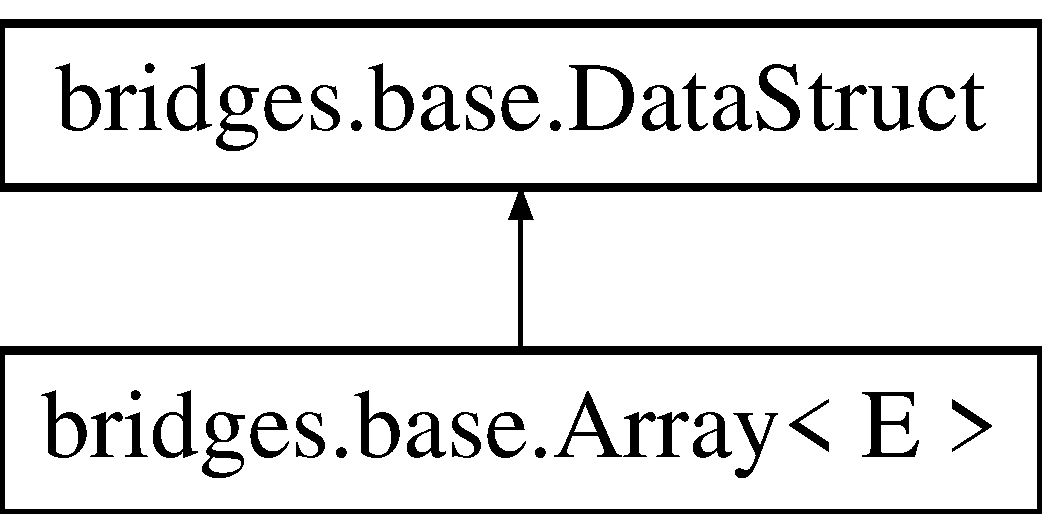
\includegraphics[height=3.000000cm]{classbridges_1_1base_1_1_array}
\end{center}
\end{figure}


\subsection{Detailed Description}
This class can be used to create arrays of type Element$<$\+E$>$. 

\begin{DoxyAuthor}{Author}
Kalpathi Subramanian
\end{DoxyAuthor}
\begin{DoxyDate}{Date}
10/8/16, 5/17/17, 5/30/18
\end{DoxyDate}
This class can be used to create arrays of type Element$<$\+E$>$ where E is a generic object representing application specific data.

This class is not directly called; instead use subclasses of arrays to construct arrays, depending on their dimension.

Arrays are internally represented as 1D arrays; currently 1D, 2D and 3D arrays are supported.


\begin{DoxyParams}{Parameters}
{\em $<$\+E$>$} & The generic parameter object that is part of this element, representing application specific data.\\
\hline
\end{DoxyParams}
\begin{DoxySeeAlso}{See also}
Example Tutorial at ~\newline
 \href{http://bridgesuncc.github.io/tutorials/Array.html}{\tt http\+://bridgesuncc.\+github.\+io/tutorials/\+Array.\+html} (1D, 2D, and 3D \hyperlink{classbridges_1_1base_1_1_array}{Array})~\newline
 
\end{DoxySeeAlso}
\subsection*{Public Member Functions}
\begin{DoxyCompactItemize}
\item 
\hyperlink{classbridges_1_1base_1_1_array_ad5dbf7bbd9811c2dac16a5c135465d4b}{Array} ()
\item 
\hyperlink{classbridges_1_1base_1_1_array_ab37dbe6efe0c34242456971e430763f7}{Array} (int num\+\_\+dims, int\mbox{[}$\,$\mbox{]} dims)
\item 
String \hyperlink{classbridges_1_1base_1_1_array_ad138b9787d46d053d6bd324b344be9a6}{get\+Data\+Struct\+Type} ()
\item 
void \hyperlink{classbridges_1_1base_1_1_array_ab7859668a25d16adfdb308e24c7d44c6}{set\+Num\+Dimensions} (int nd)
\item 
int \hyperlink{classbridges_1_1base_1_1_array_a808da9a62df3f0e7a905ec895a82087a}{get\+Num\+Dimensions} ()
\item 
void \hyperlink{classbridges_1_1base_1_1_array_aa357b6b957eeedfdb5acc9d653d7260f}{set\+Size} (int nd, int\mbox{[}$\,$\mbox{]} dim)
\begin{DoxyCompactList}\small\item\em Set the size of each dimensions; also allocates array space. \end{DoxyCompactList}\item 
void \hyperlink{classbridges_1_1base_1_1_array_af7aa7f3f18989af5f48a2b69cb7fb07d}{get\+Dimensions} (int\mbox{[}$\,$\mbox{]} dim)
\begin{DoxyCompactList}\small\item\em Get the size of each dimensions;. \end{DoxyCompactList}\item 
int \hyperlink{classbridges_1_1base_1_1_array_a49a3a4ea72c8315f1f14eed25071d18a}{get\+Size} ()
\item 
String \hyperlink{classbridges_1_1base_1_1_array_a111592e8b75202064bdf06d9c2234d74}{get\+Data\+Structure\+Representation} ()
\end{DoxyCompactItemize}
\subsection*{Protected Member Functions}
\begin{DoxyCompactItemize}
\item 
\hyperlink{classbridges_1_1base_1_1_element}{Element}$<$ E $>$ \hyperlink{classbridges_1_1base_1_1_array_a0e690cbe2606e44cce99b56802b63e0e}{get\+Element} (int indx)
\item 
void \hyperlink{classbridges_1_1base_1_1_array_aafde1304d602e8b0f673dd61bc00c18f}{set\+Element} (int indx, \hyperlink{classbridges_1_1base_1_1_element}{Element}$<$ E $>$ el)
\end{DoxyCompactItemize}
\subsection*{Additional Inherited Members}


\subsection{Constructor \& Destructor Documentation}
\mbox{\Hypertarget{classbridges_1_1base_1_1_array_ad5dbf7bbd9811c2dac16a5c135465d4b}\label{classbridges_1_1base_1_1_array_ad5dbf7bbd9811c2dac16a5c135465d4b}} 
\index{bridges\+::base\+::\+Array@{bridges\+::base\+::\+Array}!Array@{Array}}
\index{Array@{Array}!bridges\+::base\+::\+Array@{bridges\+::base\+::\+Array}}
\subsubsection{\texorpdfstring{Array()}{Array()}\hspace{0.1cm}{\footnotesize\ttfamily [1/2]}}
{\footnotesize\ttfamily \hyperlink{classbridges_1_1base_1_1_array}{bridges.\+base.\+Array}$<$ E $>$.\hyperlink{classbridges_1_1base_1_1_array}{Array} (\begin{DoxyParamCaption}{ }\end{DoxyParamCaption})}

\mbox{\Hypertarget{classbridges_1_1base_1_1_array_ab37dbe6efe0c34242456971e430763f7}\label{classbridges_1_1base_1_1_array_ab37dbe6efe0c34242456971e430763f7}} 
\index{bridges\+::base\+::\+Array@{bridges\+::base\+::\+Array}!Array@{Array}}
\index{Array@{Array}!bridges\+::base\+::\+Array@{bridges\+::base\+::\+Array}}
\subsubsection{\texorpdfstring{Array()}{Array()}\hspace{0.1cm}{\footnotesize\ttfamily [2/2]}}
{\footnotesize\ttfamily \hyperlink{classbridges_1_1base_1_1_array}{bridges.\+base.\+Array}$<$ E $>$.\hyperlink{classbridges_1_1base_1_1_array}{Array} (\begin{DoxyParamCaption}\item[{int}]{num\+\_\+dims,  }\item[{int \mbox{[}$\,$\mbox{]}}]{dims }\end{DoxyParamCaption})}

Create an array object with the specified dimensions


\begin{DoxyParams}{Parameters}
{\em num\+\_\+dims} & number of dimensions of the array \\
\hline
{\em dims} & size of each dimension \\
\hline
\end{DoxyParams}


\subsection{Member Function Documentation}
\mbox{\Hypertarget{classbridges_1_1base_1_1_array_ad138b9787d46d053d6bd324b344be9a6}\label{classbridges_1_1base_1_1_array_ad138b9787d46d053d6bd324b344be9a6}} 
\index{bridges\+::base\+::\+Array@{bridges\+::base\+::\+Array}!get\+Data\+Struct\+Type@{get\+Data\+Struct\+Type}}
\index{get\+Data\+Struct\+Type@{get\+Data\+Struct\+Type}!bridges\+::base\+::\+Array@{bridges\+::base\+::\+Array}}
\subsubsection{\texorpdfstring{get\+Data\+Struct\+Type()}{getDataStructType()}}
{\footnotesize\ttfamily String \hyperlink{classbridges_1_1base_1_1_array}{bridges.\+base.\+Array}$<$ E $>$.get\+Data\+Struct\+Type (\begin{DoxyParamCaption}{ }\end{DoxyParamCaption})}

This method gets the data structure type

\begin{DoxyReturn}{Returns}
The date structure type as a string 
\end{DoxyReturn}
\mbox{\Hypertarget{classbridges_1_1base_1_1_array_a111592e8b75202064bdf06d9c2234d74}\label{classbridges_1_1base_1_1_array_a111592e8b75202064bdf06d9c2234d74}} 
\index{bridges\+::base\+::\+Array@{bridges\+::base\+::\+Array}!get\+Data\+Structure\+Representation@{get\+Data\+Structure\+Representation}}
\index{get\+Data\+Structure\+Representation@{get\+Data\+Structure\+Representation}!bridges\+::base\+::\+Array@{bridges\+::base\+::\+Array}}
\subsubsection{\texorpdfstring{get\+Data\+Structure\+Representation()}{getDataStructureRepresentation()}}
{\footnotesize\ttfamily String \hyperlink{classbridges_1_1base_1_1_array}{bridges.\+base.\+Array}$<$ E $>$.get\+Data\+Structure\+Representation (\begin{DoxyParamCaption}{ }\end{DoxyParamCaption})}

Gets the data structure representation of the array (as J\+S\+ON)

\begin{DoxyReturn}{Returns}
array representation as a J\+S\+ON 
\end{DoxyReturn}
\mbox{\Hypertarget{classbridges_1_1base_1_1_array_af7aa7f3f18989af5f48a2b69cb7fb07d}\label{classbridges_1_1base_1_1_array_af7aa7f3f18989af5f48a2b69cb7fb07d}} 
\index{bridges\+::base\+::\+Array@{bridges\+::base\+::\+Array}!get\+Dimensions@{get\+Dimensions}}
\index{get\+Dimensions@{get\+Dimensions}!bridges\+::base\+::\+Array@{bridges\+::base\+::\+Array}}
\subsubsection{\texorpdfstring{get\+Dimensions()}{getDimensions()}}
{\footnotesize\ttfamily void \hyperlink{classbridges_1_1base_1_1_array}{bridges.\+base.\+Array}$<$ E $>$.get\+Dimensions (\begin{DoxyParamCaption}\item[{int \mbox{[}$\,$\mbox{]}}]{dim }\end{DoxyParamCaption})}



Get the size of each dimensions;. 

\begin{DoxyReturn}{Returns}
dim\mbox{[}\mbox{]} size of each dimension is returned 
\end{DoxyReturn}
\mbox{\Hypertarget{classbridges_1_1base_1_1_array_a0e690cbe2606e44cce99b56802b63e0e}\label{classbridges_1_1base_1_1_array_a0e690cbe2606e44cce99b56802b63e0e}} 
\index{bridges\+::base\+::\+Array@{bridges\+::base\+::\+Array}!get\+Element@{get\+Element}}
\index{get\+Element@{get\+Element}!bridges\+::base\+::\+Array@{bridges\+::base\+::\+Array}}
\subsubsection{\texorpdfstring{get\+Element()}{getElement()}}
{\footnotesize\ttfamily \hyperlink{classbridges_1_1base_1_1_element}{Element}$<$E$>$ \hyperlink{classbridges_1_1base_1_1_array}{bridges.\+base.\+Array}$<$ E $>$.get\+Element (\begin{DoxyParamCaption}\item[{int}]{indx }\end{DoxyParamCaption})\hspace{0.3cm}{\ttfamily [protected]}}

Get the object at \textquotesingle{}indx\textquotesingle{}


\begin{DoxyParams}{Parameters}
{\em indx} & index into the array \\
\hline
\end{DoxyParams}
\begin{DoxyReturn}{Returns}
Element$<$\+E$>$ object at \textquotesingle{}indx\textquotesingle{} 
\end{DoxyReturn}
\mbox{\Hypertarget{classbridges_1_1base_1_1_array_a808da9a62df3f0e7a905ec895a82087a}\label{classbridges_1_1base_1_1_array_a808da9a62df3f0e7a905ec895a82087a}} 
\index{bridges\+::base\+::\+Array@{bridges\+::base\+::\+Array}!get\+Num\+Dimensions@{get\+Num\+Dimensions}}
\index{get\+Num\+Dimensions@{get\+Num\+Dimensions}!bridges\+::base\+::\+Array@{bridges\+::base\+::\+Array}}
\subsubsection{\texorpdfstring{get\+Num\+Dimensions()}{getNumDimensions()}}
{\footnotesize\ttfamily int \hyperlink{classbridges_1_1base_1_1_array}{bridges.\+base.\+Array}$<$ E $>$.get\+Num\+Dimensions (\begin{DoxyParamCaption}{ }\end{DoxyParamCaption})}

Get the number of dimensions of the array;

\begin{DoxyReturn}{Returns}
number of dimensions 
\end{DoxyReturn}
\mbox{\Hypertarget{classbridges_1_1base_1_1_array_a49a3a4ea72c8315f1f14eed25071d18a}\label{classbridges_1_1base_1_1_array_a49a3a4ea72c8315f1f14eed25071d18a}} 
\index{bridges\+::base\+::\+Array@{bridges\+::base\+::\+Array}!get\+Size@{get\+Size}}
\index{get\+Size@{get\+Size}!bridges\+::base\+::\+Array@{bridges\+::base\+::\+Array}}
\subsubsection{\texorpdfstring{get\+Size()}{getSize()}}
{\footnotesize\ttfamily int \hyperlink{classbridges_1_1base_1_1_array}{bridges.\+base.\+Array}$<$ E $>$.get\+Size (\begin{DoxyParamCaption}{ }\end{DoxyParamCaption})}

Get the array size

\begin{DoxyReturn}{Returns}
size of the array 
\end{DoxyReturn}
\mbox{\Hypertarget{classbridges_1_1base_1_1_array_aafde1304d602e8b0f673dd61bc00c18f}\label{classbridges_1_1base_1_1_array_aafde1304d602e8b0f673dd61bc00c18f}} 
\index{bridges\+::base\+::\+Array@{bridges\+::base\+::\+Array}!set\+Element@{set\+Element}}
\index{set\+Element@{set\+Element}!bridges\+::base\+::\+Array@{bridges\+::base\+::\+Array}}
\subsubsection{\texorpdfstring{set\+Element()}{setElement()}}
{\footnotesize\ttfamily void \hyperlink{classbridges_1_1base_1_1_array}{bridges.\+base.\+Array}$<$ E $>$.set\+Element (\begin{DoxyParamCaption}\item[{int}]{indx,  }\item[{\hyperlink{classbridges_1_1base_1_1_element}{Element}$<$ E $>$}]{el }\end{DoxyParamCaption})\hspace{0.3cm}{\ttfamily [protected]}}

Set the input object at \textquotesingle{}indx\textquotesingle{} -\/ for 1D array


\begin{DoxyParams}{Parameters}
{\em indx} & index into the array \\
\hline
{\em el} & element object to be assigned at \textquotesingle{}indx\textquotesingle{} \\
\hline
\end{DoxyParams}
\mbox{\Hypertarget{classbridges_1_1base_1_1_array_ab7859668a25d16adfdb308e24c7d44c6}\label{classbridges_1_1base_1_1_array_ab7859668a25d16adfdb308e24c7d44c6}} 
\index{bridges\+::base\+::\+Array@{bridges\+::base\+::\+Array}!set\+Num\+Dimensions@{set\+Num\+Dimensions}}
\index{set\+Num\+Dimensions@{set\+Num\+Dimensions}!bridges\+::base\+::\+Array@{bridges\+::base\+::\+Array}}
\subsubsection{\texorpdfstring{set\+Num\+Dimensions()}{setNumDimensions()}}
{\footnotesize\ttfamily void \hyperlink{classbridges_1_1base_1_1_array}{bridges.\+base.\+Array}$<$ E $>$.set\+Num\+Dimensions (\begin{DoxyParamCaption}\item[{int}]{nd }\end{DoxyParamCaption})}

Set the number of dimensions of the array;


\begin{DoxyParams}{Parameters}
{\em nd} & number of dimensions \\
\hline
\end{DoxyParams}
\mbox{\Hypertarget{classbridges_1_1base_1_1_array_aa357b6b957eeedfdb5acc9d653d7260f}\label{classbridges_1_1base_1_1_array_aa357b6b957eeedfdb5acc9d653d7260f}} 
\index{bridges\+::base\+::\+Array@{bridges\+::base\+::\+Array}!set\+Size@{set\+Size}}
\index{set\+Size@{set\+Size}!bridges\+::base\+::\+Array@{bridges\+::base\+::\+Array}}
\subsubsection{\texorpdfstring{set\+Size()}{setSize()}}
{\footnotesize\ttfamily void \hyperlink{classbridges_1_1base_1_1_array}{bridges.\+base.\+Array}$<$ E $>$.set\+Size (\begin{DoxyParamCaption}\item[{int}]{nd,  }\item[{int \mbox{[}$\,$\mbox{]}}]{dim }\end{DoxyParamCaption})}



Set the size of each dimensions; also allocates array space. 


\begin{DoxyParams}{Parameters}
{\em nd} & number of dimension \\
\hline
{\em dim} & size of each dimension \\
\hline
\end{DoxyParams}


The documentation for this class was generated from the following file\+:\begin{DoxyCompactItemize}
\item 
/home/erik/work/bridges/bridges-\/java/src/main/java/bridges/base/\hyperlink{_array_8java}{Array.\+java}\end{DoxyCompactItemize}

\hypertarget{classbridges_1_1base_1_1_array_element}{}\section{bridges.\+base.\+Array\+Element$<$ E $>$ Class Template Reference}
\label{classbridges_1_1base_1_1_array_element}\index{bridges.\+base.\+Array\+Element$<$ E $>$@{bridges.\+base.\+Array\+Element$<$ E $>$}}
Inheritance diagram for bridges.\+base.\+Array\+Element$<$ E $>$\+:\begin{figure}[H]
\begin{center}
\leavevmode
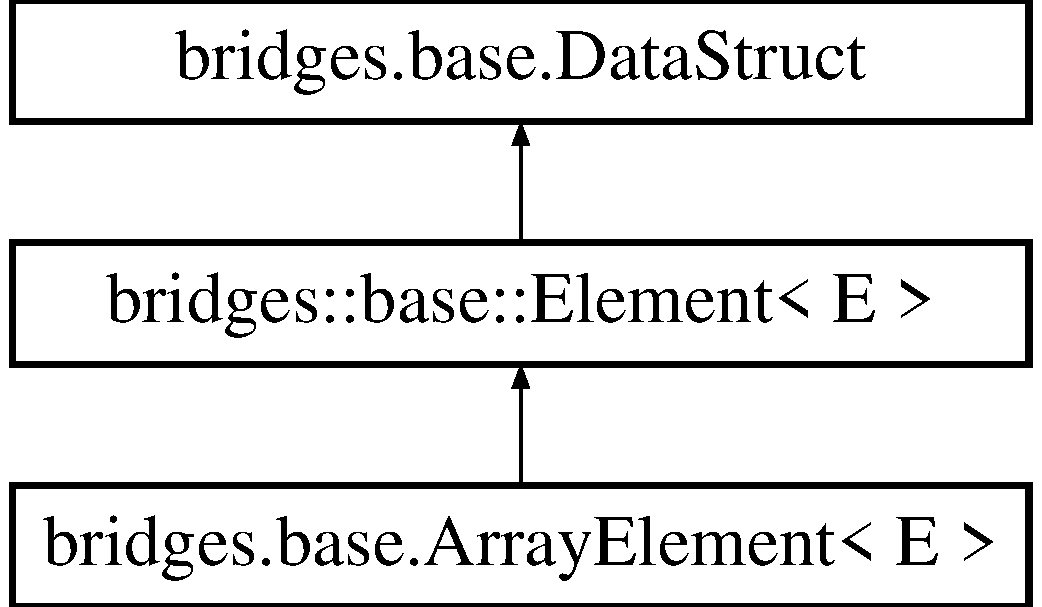
\includegraphics[height=3.000000cm]{classbridges_1_1base_1_1_array_element}
\end{center}
\end{figure}
\subsection*{Public Member Functions}
\begin{DoxyCompactItemize}
\item 
\hyperlink{classbridges_1_1base_1_1_array_element_a90cbba952d50ff26fd2b89e9f3f81322}{Array\+Element} (String label, E type)
\item 
String \hyperlink{classbridges_1_1base_1_1_array_element_a1d4f3fae7bd986237e364c2cce0bea77}{get\+Data\+Struct\+Type} ()
\end{DoxyCompactItemize}
\subsection*{Static Public Attributes}
\begin{DoxyCompactItemize}
\item 
static int \hyperlink{classbridges_1_1base_1_1_array_element_a79c69e5046da8c297026d1e457a23182}{index}
\end{DoxyCompactItemize}
\subsection*{Additional Inherited Members}


\subsection{Detailed Description}
\begin{DoxyAuthor}{Author}
Mihai Mehedint 
\end{DoxyAuthor}

\begin{DoxyParams}{Parameters}
{\em $<$\+E$>$} & This class can be used to create arrays with generic types as follows\+: Array\+Element$<$\+E$>$\mbox{[}\mbox{]} my\+Array = (Array\+Element$<$\+E$>$\mbox{[}\mbox{]}) new \hyperlink{classbridges_1_1base_1_1_array_element}{Array\+Element}\mbox{[}10\mbox{]}; Where E is\+: Tweet, Actor, Movie, Integer, String or other generic type \\
\hline
\end{DoxyParams}


\subsection{Constructor \& Destructor Documentation}
\hypertarget{classbridges_1_1base_1_1_array_element_a90cbba952d50ff26fd2b89e9f3f81322}{}\label{classbridges_1_1base_1_1_array_element_a90cbba952d50ff26fd2b89e9f3f81322} 
\index{bridges\+::base\+::\+Array\+Element@{bridges\+::base\+::\+Array\+Element}!Array\+Element@{Array\+Element}}
\index{Array\+Element@{Array\+Element}!bridges\+::base\+::\+Array\+Element@{bridges\+::base\+::\+Array\+Element}}
\subsubsection{\texorpdfstring{Array\+Element()}{ArrayElement()}}
{\footnotesize\ttfamily \hyperlink{classbridges_1_1base_1_1_array_element}{bridges.\+base.\+Array\+Element}$<$ E $>$.\hyperlink{classbridges_1_1base_1_1_array_element}{Array\+Element} (\begin{DoxyParamCaption}\item[{String}]{label,  }\item[{E}]{type }\end{DoxyParamCaption})}

Construct an array labeled \char`\"{}label\char`\"{} and holding elements of \char`\"{}type\char`\"{}. 
\begin{DoxyParams}{Parameters}
{\em label} & the label of \hyperlink{classbridges_1_1base_1_1_array_element}{Array\+Element} that shows up on the Bridges visualization \\
\hline
{\em type} & the type of \hyperlink{classbridges_1_1base_1_1_element}{Element} this array should be holding \\
\hline
\end{DoxyParams}


\subsection{Member Function Documentation}
\hypertarget{classbridges_1_1base_1_1_array_element_a1d4f3fae7bd986237e364c2cce0bea77}{}\label{classbridges_1_1base_1_1_array_element_a1d4f3fae7bd986237e364c2cce0bea77} 
\index{bridges\+::base\+::\+Array\+Element@{bridges\+::base\+::\+Array\+Element}!get\+Data\+Struct\+Type@{get\+Data\+Struct\+Type}}
\index{get\+Data\+Struct\+Type@{get\+Data\+Struct\+Type}!bridges\+::base\+::\+Array\+Element@{bridges\+::base\+::\+Array\+Element}}
\subsubsection{\texorpdfstring{get\+Data\+Struct\+Type()}{getDataStructType()}}
{\footnotesize\ttfamily String \hyperlink{classbridges_1_1base_1_1_array_element}{bridges.\+base.\+Array\+Element}$<$ E $>$.get\+Data\+Struct\+Type (\begin{DoxyParamCaption}{ }\end{DoxyParamCaption})}

This method gets the data structure type

\begin{DoxyReturn}{Returns}
The date structure type as a string 
\end{DoxyReturn}


\subsection{Member Data Documentation}
\hypertarget{classbridges_1_1base_1_1_array_element_a79c69e5046da8c297026d1e457a23182}{}\label{classbridges_1_1base_1_1_array_element_a79c69e5046da8c297026d1e457a23182} 
\index{bridges\+::base\+::\+Array\+Element@{bridges\+::base\+::\+Array\+Element}!index@{index}}
\index{index@{index}!bridges\+::base\+::\+Array\+Element@{bridges\+::base\+::\+Array\+Element}}
\subsubsection{\texorpdfstring{index}{index}}
{\footnotesize\ttfamily int \hyperlink{classbridges_1_1base_1_1_array_element}{bridges.\+base.\+Array\+Element}$<$ E $>$.index\hspace{0.3cm}{\ttfamily [static]}}



The documentation for this class was generated from the following file\+:\begin{DoxyCompactItemize}
\item 
link/base/\hyperlink{_array_element_8java}{Array\+Element.\+java}\end{DoxyCompactItemize}

\hypertarget{classbridges_1_1base_1_1_array_of_element}{}\section{bridges.\+base.\+Array\+Of\+Element$<$ E extends Comparable$<$?super E $>$ Class Template Reference}
\label{classbridges_1_1base_1_1_array_of_element}\index{bridges.\+base.\+Array\+Of\+Element$<$ E extends Comparable$<$?super E $>$@{bridges.\+base.\+Array\+Of\+Element$<$ E extends Comparable$<$?super E $>$}}
\subsection*{Public Member Functions}
\begin{DoxyCompactItemize}
\item 
\hyperlink{classbridges_1_1base_1_1_array_of_element_a300ff065d85567089d47d323783f6d8b}{Array\+Of\+Element} (Class$<$?$>$ e)
\end{DoxyCompactItemize}


\subsection{Detailed Description}
\begin{DoxyAuthor}{Author}
mihai This class is used to allow the Bridges Visualization to represent an array. 
\end{DoxyAuthor}


\subsection{Constructor \& Destructor Documentation}
\hypertarget{classbridges_1_1base_1_1_array_of_element_a300ff065d85567089d47d323783f6d8b}{}\index{bridges\+::base\+::\+Array\+Of\+Element@{bridges\+::base\+::\+Array\+Of\+Element}!Array\+Of\+Element@{Array\+Of\+Element}}
\index{Array\+Of\+Element@{Array\+Of\+Element}!bridges\+::base\+::\+Array\+Of\+Element@{bridges\+::base\+::\+Array\+Of\+Element}}
\subsubsection[{Array\+Of\+Element(\+Class$<$?$>$ e)}]{\setlength{\rightskip}{0pt plus 5cm}{\bf bridges.\+base.\+Array\+Of\+Element}$<$ E extends Comparable$<$?super E $>$.{\bf Array\+Of\+Element} (
\begin{DoxyParamCaption}
\item[{Class$<$?$>$}]{e}
\end{DoxyParamCaption}
)}\label{classbridges_1_1base_1_1_array_of_element_a300ff065d85567089d47d323783f6d8b}
Construct an \hyperlink{classbridges_1_1base_1_1_array_of_element}{Array\+Of\+Element} for a particular class. 
\begin{DoxyParams}{Parameters}
{\em e} & the class to make an array of (e.\+g. S\+Lelement.\+class). \\
\hline
\end{DoxyParams}


The documentation for this class was generated from the following file\+:\begin{DoxyCompactItemize}
\item 
link/base/\hyperlink{_array_of_element_8java}{Array\+Of\+Element.\+java}\end{DoxyCompactItemize}

\hypertarget{classbridges_1_1base_1_1_a_v_l_tree_element}{}\section{bridges.\+base.\+A\+V\+L\+Tree\+Element$<$ K, E $>$ Class Template Reference}
\label{classbridges_1_1base_1_1_a_v_l_tree_element}\index{bridges.\+base.\+A\+V\+L\+Tree\+Element$<$ K, E $>$@{bridges.\+base.\+A\+V\+L\+Tree\+Element$<$ K, E $>$}}
Inheritance diagram for bridges.\+base.\+A\+V\+L\+Tree\+Element$<$ K, E $>$\+:\begin{figure}[H]
\begin{center}
\leavevmode
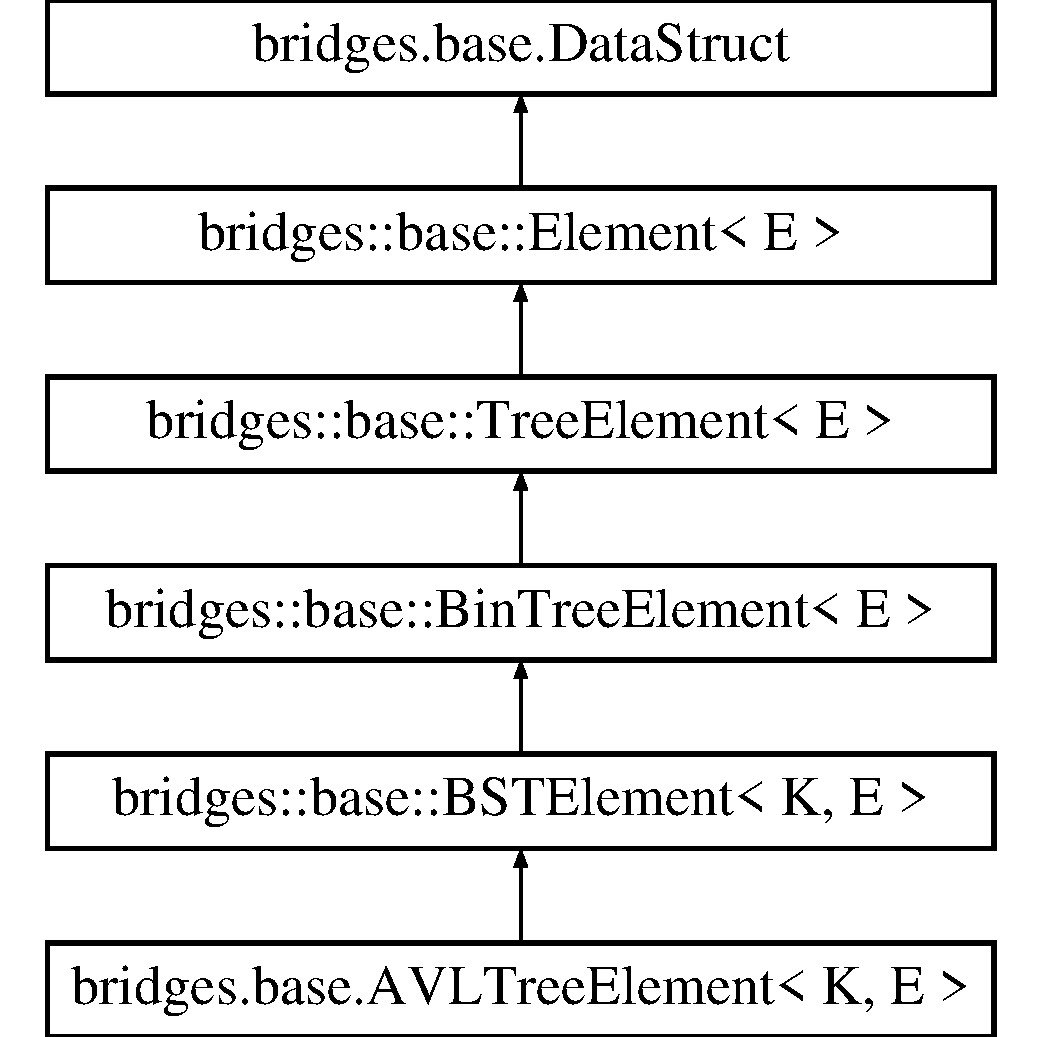
\includegraphics[height=6.000000cm]{classbridges_1_1base_1_1_a_v_l_tree_element}
\end{center}
\end{figure}


\subsection{Detailed Description}
This class extends the \mbox{\hyperlink{classbridges_1_1base_1_1_b_s_t_element}{B\+S\+T\+Element}} class by adding a height and balance factor fields that are useful in A\+VL trees. 

A\+VL tree elements include a \textquotesingle{}height\textquotesingle{} and a \textquotesingle{}bal\+Factor\textquotesingle{} value, representing the height and balance factor of the A\+VL tree at that node, respectively. This is useful in representing A\+VL trees.

A\+V\+L\+Tree elements contain a visualizer (\mbox{\hyperlink{classbridges_1_1base_1_1_element_visualizer}{Element\+Visualizer}}) object for setting visual attributes (color, shape, opacity, size), necessary for displaying them in a web browser.

A\+V\+L\+Tree elements also have a \mbox{\hyperlink{classbridges_1_1base_1_1_link_visualizer}{Link\+Visualizer}} object, that is used when they are linked to another element, appropriate for setting link attributes, for instance, between the current element and its left or right child

\begin{DoxySeeAlso}{See also}
Example tutorial using \mbox{\hyperlink{classbridges_1_1base_1_1_a_v_l_tree_element}{A\+V\+L\+Tree\+Element}} at \href{http://bridgesuncc.github.io/tutorials/AVL.html}{\tt http\+://bridgesuncc.\+github.\+io/tutorials/\+A\+V\+L.\+html}
\end{DoxySeeAlso}

\begin{DoxyParams}{Parameters}
{\em E} & the generic parameter object that is part of this element, representing application specific data. \\
\hline
{\em K} & is the search key parameter in the A\+VL tree node; K must be orderable, such as integer, float, string, etc., on which relational operators work.\\
\hline
\end{DoxyParams}
\begin{DoxyAuthor}{Author}
Kalpathi Subramanian, Mihai Mehedint
\end{DoxyAuthor}
\begin{DoxyDate}{Date}
6/22/16, 1/7/17, 5/17/17, 7/12/19 
\end{DoxyDate}
\subsection*{Public Member Functions}
\begin{DoxyCompactItemize}
\item 
\mbox{\hyperlink{classbridges_1_1base_1_1_a_v_l_tree_element_a8fe4490d3d5d16991736bd1a7243b904}{A\+V\+L\+Tree\+Element}} ()
\item 
\mbox{\hyperlink{classbridges_1_1base_1_1_a_v_l_tree_element_a060ec94b52675313ad15388e3f292df5}{A\+V\+L\+Tree\+Element}} (K k, E e)
\item 
String \mbox{\hyperlink{classbridges_1_1base_1_1_a_v_l_tree_element_abdd9e63de10732ef46bd5d531bd7f9d8}{get\+Data\+Struct\+Type}} ()
\item 
int \mbox{\hyperlink{classbridges_1_1base_1_1_a_v_l_tree_element_a52fe2886334c841547d238db69022697}{get\+Height}} ()
\item 
void \mbox{\hyperlink{classbridges_1_1base_1_1_a_v_l_tree_element_ac42b744989ed7e18dcbd52980e674b33}{set\+Height}} (int h)
\item 
int \mbox{\hyperlink{classbridges_1_1base_1_1_a_v_l_tree_element_a0478ca0351cd714e8f7b8e49703990c8}{get\+Balance\+Factor}} ()
\item 
void \mbox{\hyperlink{classbridges_1_1base_1_1_a_v_l_tree_element_a0dc3c83e750cc39535afb08ea92f6c98}{set\+Balance\+Factor}} (int bf)
\item 
\mbox{\hyperlink{classbridges_1_1base_1_1_a_v_l_tree_element}{A\+V\+L\+Tree\+Element}}$<$ K, E $>$ \mbox{\hyperlink{classbridges_1_1base_1_1_a_v_l_tree_element_a86f1329b19d2886ba7bf713e3844ecd6}{get\+Left}} ()
\item 
\mbox{\hyperlink{classbridges_1_1base_1_1_a_v_l_tree_element}{A\+V\+L\+Tree\+Element}}$<$ K, E $>$ \mbox{\hyperlink{classbridges_1_1base_1_1_a_v_l_tree_element_aab93418ac19605f2c7c57aa38d110921}{get\+Right}} ()
\item 
String \mbox{\hyperlink{classbridges_1_1base_1_1_a_v_l_tree_element_af7ab86f2421864daa4fdc2e84939f4ce}{get\+Element\+Representation}} ()
\end{DoxyCompactItemize}
\subsection*{Additional Inherited Members}


\subsection{Constructor \& Destructor Documentation}
\mbox{\Hypertarget{classbridges_1_1base_1_1_a_v_l_tree_element_a8fe4490d3d5d16991736bd1a7243b904}\label{classbridges_1_1base_1_1_a_v_l_tree_element_a8fe4490d3d5d16991736bd1a7243b904}} 
\index{bridges\+::base\+::\+A\+V\+L\+Tree\+Element@{bridges\+::base\+::\+A\+V\+L\+Tree\+Element}!A\+V\+L\+Tree\+Element@{A\+V\+L\+Tree\+Element}}
\index{A\+V\+L\+Tree\+Element@{A\+V\+L\+Tree\+Element}!bridges\+::base\+::\+A\+V\+L\+Tree\+Element@{bridges\+::base\+::\+A\+V\+L\+Tree\+Element}}
\subsubsection{\texorpdfstring{A\+V\+L\+Tree\+Element()}{AVLTreeElement()}\hspace{0.1cm}{\footnotesize\ttfamily [1/2]}}
{\footnotesize\ttfamily \mbox{\hyperlink{classbridges_1_1base_1_1_a_v_l_tree_element}{bridges.\+base.\+A\+V\+L\+Tree\+Element}}$<$ K, E $>$.\mbox{\hyperlink{classbridges_1_1base_1_1_a_v_l_tree_element}{A\+V\+L\+Tree\+Element}} (\begin{DoxyParamCaption}{ }\end{DoxyParamCaption})}

Construct an \mbox{\hyperlink{classbridges_1_1base_1_1_a_v_l_tree_element}{A\+V\+L\+Tree\+Element}} with default values \mbox{\Hypertarget{classbridges_1_1base_1_1_a_v_l_tree_element_a060ec94b52675313ad15388e3f292df5}\label{classbridges_1_1base_1_1_a_v_l_tree_element_a060ec94b52675313ad15388e3f292df5}} 
\index{bridges\+::base\+::\+A\+V\+L\+Tree\+Element@{bridges\+::base\+::\+A\+V\+L\+Tree\+Element}!A\+V\+L\+Tree\+Element@{A\+V\+L\+Tree\+Element}}
\index{A\+V\+L\+Tree\+Element@{A\+V\+L\+Tree\+Element}!bridges\+::base\+::\+A\+V\+L\+Tree\+Element@{bridges\+::base\+::\+A\+V\+L\+Tree\+Element}}
\subsubsection{\texorpdfstring{A\+V\+L\+Tree\+Element()}{AVLTreeElement()}\hspace{0.1cm}{\footnotesize\ttfamily [2/2]}}
{\footnotesize\ttfamily \mbox{\hyperlink{classbridges_1_1base_1_1_a_v_l_tree_element}{bridges.\+base.\+A\+V\+L\+Tree\+Element}}$<$ K, E $>$.\mbox{\hyperlink{classbridges_1_1base_1_1_a_v_l_tree_element}{A\+V\+L\+Tree\+Element}} (\begin{DoxyParamCaption}\item[{K}]{k,  }\item[{E}]{e }\end{DoxyParamCaption})}

Construct an \mbox{\hyperlink{classbridges_1_1base_1_1_a_v_l_tree_element}{A\+V\+L\+Tree\+Element}} holding a key value \char`\"{}k\char`\"{} and an object \char`\"{}e\char`\"{}


\begin{DoxyParams}{Parameters}
{\em k} & the search key \\
\hline
{\em e} & the appl specific object that \mbox{\hyperlink{classbridges_1_1base_1_1_element}{Element}} is holding \\
\hline
\end{DoxyParams}


\subsection{Member Function Documentation}
\mbox{\Hypertarget{classbridges_1_1base_1_1_a_v_l_tree_element_a0478ca0351cd714e8f7b8e49703990c8}\label{classbridges_1_1base_1_1_a_v_l_tree_element_a0478ca0351cd714e8f7b8e49703990c8}} 
\index{bridges\+::base\+::\+A\+V\+L\+Tree\+Element@{bridges\+::base\+::\+A\+V\+L\+Tree\+Element}!get\+Balance\+Factor@{get\+Balance\+Factor}}
\index{get\+Balance\+Factor@{get\+Balance\+Factor}!bridges\+::base\+::\+A\+V\+L\+Tree\+Element@{bridges\+::base\+::\+A\+V\+L\+Tree\+Element}}
\subsubsection{\texorpdfstring{get\+Balance\+Factor()}{getBalanceFactor()}}
{\footnotesize\ttfamily int \mbox{\hyperlink{classbridges_1_1base_1_1_a_v_l_tree_element}{bridges.\+base.\+A\+V\+L\+Tree\+Element}}$<$ K, E $>$.get\+Balance\+Factor (\begin{DoxyParamCaption}{ }\end{DoxyParamCaption})}

This method returns the balance factor of the tree at this node

\begin{DoxyReturn}{Returns}
balance factor 
\end{DoxyReturn}
\mbox{\Hypertarget{classbridges_1_1base_1_1_a_v_l_tree_element_abdd9e63de10732ef46bd5d531bd7f9d8}\label{classbridges_1_1base_1_1_a_v_l_tree_element_abdd9e63de10732ef46bd5d531bd7f9d8}} 
\index{bridges\+::base\+::\+A\+V\+L\+Tree\+Element@{bridges\+::base\+::\+A\+V\+L\+Tree\+Element}!get\+Data\+Struct\+Type@{get\+Data\+Struct\+Type}}
\index{get\+Data\+Struct\+Type@{get\+Data\+Struct\+Type}!bridges\+::base\+::\+A\+V\+L\+Tree\+Element@{bridges\+::base\+::\+A\+V\+L\+Tree\+Element}}
\subsubsection{\texorpdfstring{get\+Data\+Struct\+Type()}{getDataStructType()}}
{\footnotesize\ttfamily String \mbox{\hyperlink{classbridges_1_1base_1_1_a_v_l_tree_element}{bridges.\+base.\+A\+V\+L\+Tree\+Element}}$<$ K, E $>$.get\+Data\+Struct\+Type (\begin{DoxyParamCaption}{ }\end{DoxyParamCaption})}

This method gets the data structure type

\begin{DoxyReturn}{Returns}
The date structure type as a string 
\end{DoxyReturn}
\mbox{\Hypertarget{classbridges_1_1base_1_1_a_v_l_tree_element_af7ab86f2421864daa4fdc2e84939f4ce}\label{classbridges_1_1base_1_1_a_v_l_tree_element_af7ab86f2421864daa4fdc2e84939f4ce}} 
\index{bridges\+::base\+::\+A\+V\+L\+Tree\+Element@{bridges\+::base\+::\+A\+V\+L\+Tree\+Element}!get\+Element\+Representation@{get\+Element\+Representation}}
\index{get\+Element\+Representation@{get\+Element\+Representation}!bridges\+::base\+::\+A\+V\+L\+Tree\+Element@{bridges\+::base\+::\+A\+V\+L\+Tree\+Element}}
\subsubsection{\texorpdfstring{get\+Element\+Representation()}{getElementRepresentation()}}
{\footnotesize\ttfamily String \mbox{\hyperlink{classbridges_1_1base_1_1_a_v_l_tree_element}{bridges.\+base.\+A\+V\+L\+Tree\+Element}}$<$ K, E $>$.get\+Element\+Representation (\begin{DoxyParamCaption}{ }\end{DoxyParamCaption})}

Augment the element with the \char`\"{}height\char`\"{} and \char`\"{}balance factor\char`\"{} fields.

\begin{DoxyReturn}{Returns}
the augmented J\+S\+ON string 
\end{DoxyReturn}
\mbox{\Hypertarget{classbridges_1_1base_1_1_a_v_l_tree_element_a52fe2886334c841547d238db69022697}\label{classbridges_1_1base_1_1_a_v_l_tree_element_a52fe2886334c841547d238db69022697}} 
\index{bridges\+::base\+::\+A\+V\+L\+Tree\+Element@{bridges\+::base\+::\+A\+V\+L\+Tree\+Element}!get\+Height@{get\+Height}}
\index{get\+Height@{get\+Height}!bridges\+::base\+::\+A\+V\+L\+Tree\+Element@{bridges\+::base\+::\+A\+V\+L\+Tree\+Element}}
\subsubsection{\texorpdfstring{get\+Height()}{getHeight()}}
{\footnotesize\ttfamily int \mbox{\hyperlink{classbridges_1_1base_1_1_a_v_l_tree_element}{bridges.\+base.\+A\+V\+L\+Tree\+Element}}$<$ K, E $>$.get\+Height (\begin{DoxyParamCaption}{ }\end{DoxyParamCaption})}

This method returns the height of the tree at this node

\begin{DoxyReturn}{Returns}
height 
\end{DoxyReturn}
\mbox{\Hypertarget{classbridges_1_1base_1_1_a_v_l_tree_element_a86f1329b19d2886ba7bf713e3844ecd6}\label{classbridges_1_1base_1_1_a_v_l_tree_element_a86f1329b19d2886ba7bf713e3844ecd6}} 
\index{bridges\+::base\+::\+A\+V\+L\+Tree\+Element@{bridges\+::base\+::\+A\+V\+L\+Tree\+Element}!get\+Left@{get\+Left}}
\index{get\+Left@{get\+Left}!bridges\+::base\+::\+A\+V\+L\+Tree\+Element@{bridges\+::base\+::\+A\+V\+L\+Tree\+Element}}
\subsubsection{\texorpdfstring{get\+Left()}{getLeft()}}
{\footnotesize\ttfamily \mbox{\hyperlink{classbridges_1_1base_1_1_a_v_l_tree_element}{A\+V\+L\+Tree\+Element}}$<$K, E$>$ \mbox{\hyperlink{classbridges_1_1base_1_1_a_v_l_tree_element}{bridges.\+base.\+A\+V\+L\+Tree\+Element}}$<$ K, E $>$.get\+Left (\begin{DoxyParamCaption}{ }\end{DoxyParamCaption})}

This method returns the left child of the tree node

\begin{DoxyReturn}{Returns}
the left child of this node 
\end{DoxyReturn}
\mbox{\Hypertarget{classbridges_1_1base_1_1_a_v_l_tree_element_aab93418ac19605f2c7c57aa38d110921}\label{classbridges_1_1base_1_1_a_v_l_tree_element_aab93418ac19605f2c7c57aa38d110921}} 
\index{bridges\+::base\+::\+A\+V\+L\+Tree\+Element@{bridges\+::base\+::\+A\+V\+L\+Tree\+Element}!get\+Right@{get\+Right}}
\index{get\+Right@{get\+Right}!bridges\+::base\+::\+A\+V\+L\+Tree\+Element@{bridges\+::base\+::\+A\+V\+L\+Tree\+Element}}
\subsubsection{\texorpdfstring{get\+Right()}{getRight()}}
{\footnotesize\ttfamily \mbox{\hyperlink{classbridges_1_1base_1_1_a_v_l_tree_element}{A\+V\+L\+Tree\+Element}}$<$K, E$>$ \mbox{\hyperlink{classbridges_1_1base_1_1_a_v_l_tree_element}{bridges.\+base.\+A\+V\+L\+Tree\+Element}}$<$ K, E $>$.get\+Right (\begin{DoxyParamCaption}{ }\end{DoxyParamCaption})}

This method returns the right child of tree node

\begin{DoxyReturn}{Returns}
the right child of this node 
\end{DoxyReturn}
\mbox{\Hypertarget{classbridges_1_1base_1_1_a_v_l_tree_element_a0dc3c83e750cc39535afb08ea92f6c98}\label{classbridges_1_1base_1_1_a_v_l_tree_element_a0dc3c83e750cc39535afb08ea92f6c98}} 
\index{bridges\+::base\+::\+A\+V\+L\+Tree\+Element@{bridges\+::base\+::\+A\+V\+L\+Tree\+Element}!set\+Balance\+Factor@{set\+Balance\+Factor}}
\index{set\+Balance\+Factor@{set\+Balance\+Factor}!bridges\+::base\+::\+A\+V\+L\+Tree\+Element@{bridges\+::base\+::\+A\+V\+L\+Tree\+Element}}
\subsubsection{\texorpdfstring{set\+Balance\+Factor()}{setBalanceFactor()}}
{\footnotesize\ttfamily void \mbox{\hyperlink{classbridges_1_1base_1_1_a_v_l_tree_element}{bridges.\+base.\+A\+V\+L\+Tree\+Element}}$<$ K, E $>$.set\+Balance\+Factor (\begin{DoxyParamCaption}\item[{int}]{bf }\end{DoxyParamCaption})}

This method sets the balance factor of the tree at this node


\begin{DoxyParams}{Parameters}
{\em bf} & balance factor \\
\hline
\end{DoxyParams}
\mbox{\Hypertarget{classbridges_1_1base_1_1_a_v_l_tree_element_ac42b744989ed7e18dcbd52980e674b33}\label{classbridges_1_1base_1_1_a_v_l_tree_element_ac42b744989ed7e18dcbd52980e674b33}} 
\index{bridges\+::base\+::\+A\+V\+L\+Tree\+Element@{bridges\+::base\+::\+A\+V\+L\+Tree\+Element}!set\+Height@{set\+Height}}
\index{set\+Height@{set\+Height}!bridges\+::base\+::\+A\+V\+L\+Tree\+Element@{bridges\+::base\+::\+A\+V\+L\+Tree\+Element}}
\subsubsection{\texorpdfstring{set\+Height()}{setHeight()}}
{\footnotesize\ttfamily void \mbox{\hyperlink{classbridges_1_1base_1_1_a_v_l_tree_element}{bridges.\+base.\+A\+V\+L\+Tree\+Element}}$<$ K, E $>$.set\+Height (\begin{DoxyParamCaption}\item[{int}]{h }\end{DoxyParamCaption})}

This method sets the height of the tree at this node


\begin{DoxyParams}{Parameters}
{\em h} & height \\
\hline
\end{DoxyParams}


The documentation for this class was generated from the following file\+:\begin{DoxyCompactItemize}
\item 
/\+Users/kalpathi/gr/bridges/client/java/src/main/java/bridges/base/\mbox{\hyperlink{_a_v_l_tree_element_8java}{A\+V\+L\+Tree\+Element.\+java}}\end{DoxyCompactItemize}

\hypertarget{classbridges_1_1base_1_1_bin_tree_element}{}\section{bridges.\+base.\+Bin\+Tree\+Element$<$ E $>$ Class Template Reference}
\label{classbridges_1_1base_1_1_bin_tree_element}\index{bridges.\+base.\+Bin\+Tree\+Element$<$ E $>$@{bridges.\+base.\+Bin\+Tree\+Element$<$ E $>$}}


This class is extended from the \hyperlink{classbridges_1_1base_1_1_tree_element}{Tree\+Element} class and can be used to create binary tree element objects.  


Inheritance diagram for bridges.\+base.\+Bin\+Tree\+Element$<$ E $>$\+:\begin{figure}[H]
\begin{center}
\leavevmode
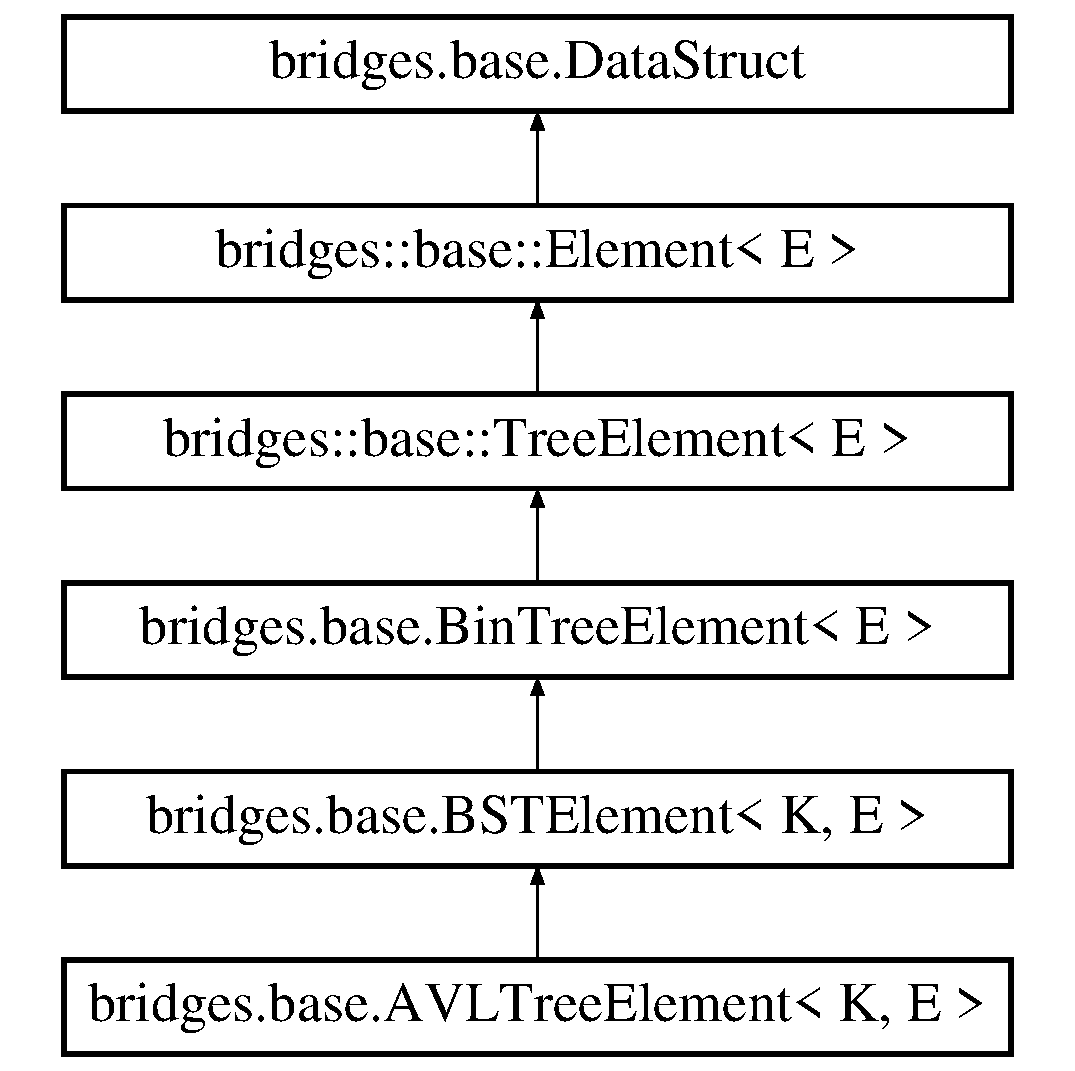
\includegraphics[height=6.000000cm]{classbridges_1_1base_1_1_bin_tree_element}
\end{center}
\end{figure}
\subsection*{Public Member Functions}
\begin{DoxyCompactItemize}
\item 
\hyperlink{classbridges_1_1base_1_1_bin_tree_element_ad6dbf38d53a78be561039c46bde8bc47}{Bin\+Tree\+Element} ()
\item 
\hyperlink{classbridges_1_1base_1_1_bin_tree_element_a2d31fa068f962ced8702fdb4b36c9186}{Bin\+Tree\+Element} (E e)
\item 
\hyperlink{classbridges_1_1base_1_1_bin_tree_element_aac0e300f53d5c1c89b747a1f2c5d54c9}{Bin\+Tree\+Element} (String label, E e)
\item 
\hyperlink{classbridges_1_1base_1_1_bin_tree_element_ab402fac72353087b1b93e82db007e1d7}{Bin\+Tree\+Element} (\hyperlink{classbridges_1_1base_1_1_bin_tree_element}{Bin\+Tree\+Element}$<$ E $>$ left, \hyperlink{classbridges_1_1base_1_1_bin_tree_element}{Bin\+Tree\+Element}$<$ E $>$ right)
\item 
\hyperlink{classbridges_1_1base_1_1_bin_tree_element_a37f3def3cdf4a9eccf577d0ff3c704e9}{Bin\+Tree\+Element} (E e, \hyperlink{classbridges_1_1base_1_1_bin_tree_element}{Bin\+Tree\+Element}$<$ E $>$ left, \hyperlink{classbridges_1_1base_1_1_bin_tree_element}{Bin\+Tree\+Element}$<$ E $>$ right)
\item 
String \hyperlink{classbridges_1_1base_1_1_bin_tree_element_a60fa936692e168f70fb8567090c98883}{get\+Data\+Struct\+Type} ()
\item 
\hyperlink{classbridges_1_1base_1_1_bin_tree_element}{Bin\+Tree\+Element}$<$ E $>$ \hyperlink{classbridges_1_1base_1_1_bin_tree_element_aeb6fd894af8e158c9c48dd0749d1bd22}{get\+Left} ()
\item 
void \hyperlink{classbridges_1_1base_1_1_bin_tree_element_a5bcc2c1374a49f7ab2523ce53d204c30}{set\+Left} (\hyperlink{classbridges_1_1base_1_1_bin_tree_element}{Bin\+Tree\+Element}$<$ E $>$ left)
\item 
\hyperlink{classbridges_1_1base_1_1_bin_tree_element}{Bin\+Tree\+Element}$<$ E $>$ \hyperlink{classbridges_1_1base_1_1_bin_tree_element_aa3855c26617ada7248a9d4f83cf455b7}{get\+Right} ()
\item 
void \hyperlink{classbridges_1_1base_1_1_bin_tree_element_abc40e3ed4cfaf4b74aacfd3657e89ebc}{set\+Right} (\hyperlink{classbridges_1_1base_1_1_bin_tree_element}{Bin\+Tree\+Element}$<$ E $>$ right)
\end{DoxyCompactItemize}
\subsection*{Additional Inherited Members}


\subsection{Detailed Description}
This class is extended from the \hyperlink{classbridges_1_1base_1_1_tree_element}{Tree\+Element} class and can be used to create binary tree element objects. 

The Bin\+Tree element class is the building block for creating binary tree structures. It contains two children (viz., left, right).

\hyperlink{classbridges_1_1base_1_1_bin_tree_element}{Bin\+Tree\+Element} contains a visualizer (\hyperlink{classbridges_1_1base_1_1_element_visualizer}{Element\+Visualizer}) object for setting visual attributes (color, shape, opacity, size), necessary for displaying them in a web browser.

Elements also have a \hyperlink{classbridges_1_1base_1_1_link_visualizer}{Link\+Visualizer} object, that is used when they are linked to another element, appropriate for setting link attributes, for instance, between the current element and its left or right child


\begin{DoxyParams}{Parameters}
{\em E} & he generic parameter object that is part of this element, representing application specific data.\\
\hline
\end{DoxyParams}
\begin{DoxyAuthor}{Author}
Kalpathi Subramanian, Mihai Mehedint
\end{DoxyAuthor}
\begin{DoxyDate}{Date}
6/22/16, 1/7/17, 5/17/17
\end{DoxyDate}
\begin{DoxySeeAlso}{See also}
Example Tutorial at ~\newline
 \href{http://bridgesuncc.github.io/Hello_World_Tutorials/BTree.html}{\tt http\+://bridgesuncc.\+github.\+io/\+Hello\+\_\+\+World\+\_\+\+Tutorials/\+B\+Tree.\+html} 
\end{DoxySeeAlso}


\subsection{Constructor \& Destructor Documentation}
\hypertarget{classbridges_1_1base_1_1_bin_tree_element_ad6dbf38d53a78be561039c46bde8bc47}{}\label{classbridges_1_1base_1_1_bin_tree_element_ad6dbf38d53a78be561039c46bde8bc47} 
\index{bridges\+::base\+::\+Bin\+Tree\+Element@{bridges\+::base\+::\+Bin\+Tree\+Element}!Bin\+Tree\+Element@{Bin\+Tree\+Element}}
\index{Bin\+Tree\+Element@{Bin\+Tree\+Element}!bridges\+::base\+::\+Bin\+Tree\+Element@{bridges\+::base\+::\+Bin\+Tree\+Element}}
\subsubsection{\texorpdfstring{Bin\+Tree\+Element()}{BinTreeElement()}\hspace{0.1cm}{\footnotesize\ttfamily [1/5]}}
{\footnotesize\ttfamily \hyperlink{classbridges_1_1base_1_1_bin_tree_element}{bridges.\+base.\+Bin\+Tree\+Element}$<$ E $>$.\hyperlink{classbridges_1_1base_1_1_bin_tree_element}{Bin\+Tree\+Element} (\begin{DoxyParamCaption}{ }\end{DoxyParamCaption})}

Constructs an empty Binary Tree \hyperlink{classbridges_1_1base_1_1_element}{Element} with right and left pointers set to null. \hypertarget{classbridges_1_1base_1_1_bin_tree_element_a2d31fa068f962ced8702fdb4b36c9186}{}\label{classbridges_1_1base_1_1_bin_tree_element_a2d31fa068f962ced8702fdb4b36c9186} 
\index{bridges\+::base\+::\+Bin\+Tree\+Element@{bridges\+::base\+::\+Bin\+Tree\+Element}!Bin\+Tree\+Element@{Bin\+Tree\+Element}}
\index{Bin\+Tree\+Element@{Bin\+Tree\+Element}!bridges\+::base\+::\+Bin\+Tree\+Element@{bridges\+::base\+::\+Bin\+Tree\+Element}}
\subsubsection{\texorpdfstring{Bin\+Tree\+Element()}{BinTreeElement()}\hspace{0.1cm}{\footnotesize\ttfamily [2/5]}}
{\footnotesize\ttfamily \hyperlink{classbridges_1_1base_1_1_bin_tree_element}{bridges.\+base.\+Bin\+Tree\+Element}$<$ E $>$.\hyperlink{classbridges_1_1base_1_1_bin_tree_element}{Bin\+Tree\+Element} (\begin{DoxyParamCaption}\item[{E}]{e }\end{DoxyParamCaption})}

Constructs a \hyperlink{classbridges_1_1base_1_1_tree_element}{Tree\+Element} holding an object \char`\"{}e\char`\"{} with right and left pointers set to null.


\begin{DoxyParams}{Parameters}
{\em e} & the generic object that \hyperlink{classbridges_1_1base_1_1_tree_element}{Tree\+Element} will hold \\
\hline
\end{DoxyParams}
\hypertarget{classbridges_1_1base_1_1_bin_tree_element_aac0e300f53d5c1c89b747a1f2c5d54c9}{}\label{classbridges_1_1base_1_1_bin_tree_element_aac0e300f53d5c1c89b747a1f2c5d54c9} 
\index{bridges\+::base\+::\+Bin\+Tree\+Element@{bridges\+::base\+::\+Bin\+Tree\+Element}!Bin\+Tree\+Element@{Bin\+Tree\+Element}}
\index{Bin\+Tree\+Element@{Bin\+Tree\+Element}!bridges\+::base\+::\+Bin\+Tree\+Element@{bridges\+::base\+::\+Bin\+Tree\+Element}}
\subsubsection{\texorpdfstring{Bin\+Tree\+Element()}{BinTreeElement()}\hspace{0.1cm}{\footnotesize\ttfamily [3/5]}}
{\footnotesize\ttfamily \hyperlink{classbridges_1_1base_1_1_bin_tree_element}{bridges.\+base.\+Bin\+Tree\+Element}$<$ E $>$.\hyperlink{classbridges_1_1base_1_1_bin_tree_element}{Bin\+Tree\+Element} (\begin{DoxyParamCaption}\item[{String}]{label,  }\item[{E}]{e }\end{DoxyParamCaption})}

Constructs a \hyperlink{classbridges_1_1base_1_1_tree_element}{Tree\+Element} with label set to \char`\"{}label\char`\"{}, holding an object \char`\"{}e\char`\"{}.


\begin{DoxyParams}{Parameters}
{\em label} & the label of \hyperlink{classbridges_1_1base_1_1_tree_element}{Tree\+Element} that shows up on the Bridges visualization\\
\hline
{\em e} & the generic object that \hyperlink{classbridges_1_1base_1_1_tree_element}{Tree\+Element} will hold \\
\hline
\end{DoxyParams}
\hypertarget{classbridges_1_1base_1_1_bin_tree_element_ab402fac72353087b1b93e82db007e1d7}{}\label{classbridges_1_1base_1_1_bin_tree_element_ab402fac72353087b1b93e82db007e1d7} 
\index{bridges\+::base\+::\+Bin\+Tree\+Element@{bridges\+::base\+::\+Bin\+Tree\+Element}!Bin\+Tree\+Element@{Bin\+Tree\+Element}}
\index{Bin\+Tree\+Element@{Bin\+Tree\+Element}!bridges\+::base\+::\+Bin\+Tree\+Element@{bridges\+::base\+::\+Bin\+Tree\+Element}}
\subsubsection{\texorpdfstring{Bin\+Tree\+Element()}{BinTreeElement()}\hspace{0.1cm}{\footnotesize\ttfamily [4/5]}}
{\footnotesize\ttfamily \hyperlink{classbridges_1_1base_1_1_bin_tree_element}{bridges.\+base.\+Bin\+Tree\+Element}$<$ E $>$.\hyperlink{classbridges_1_1base_1_1_bin_tree_element}{Bin\+Tree\+Element} (\begin{DoxyParamCaption}\item[{\hyperlink{classbridges_1_1base_1_1_bin_tree_element}{Bin\+Tree\+Element}$<$ E $>$}]{left,  }\item[{\hyperlink{classbridges_1_1base_1_1_bin_tree_element}{Bin\+Tree\+Element}$<$ E $>$}]{right }\end{DoxyParamCaption})}

Constructs an empty \hyperlink{classbridges_1_1base_1_1_tree_element}{Tree\+Element} left pointer pointing to \char`\"{}left\char`\"{} and right pointer pointing to \char`\"{}right\char`\"{}.


\begin{DoxyParams}{Parameters}
{\em left} & the \hyperlink{classbridges_1_1base_1_1_tree_element}{Tree\+Element} to be assigned to the left pointer of this \hyperlink{classbridges_1_1base_1_1_tree_element}{Tree\+Element} \\
\hline
{\em right} & the \hyperlink{classbridges_1_1base_1_1_tree_element}{Tree\+Element} to be assigned to the right pointer of this \hyperlink{classbridges_1_1base_1_1_tree_element}{Tree\+Element} \\
\hline
\end{DoxyParams}
\hypertarget{classbridges_1_1base_1_1_bin_tree_element_a37f3def3cdf4a9eccf577d0ff3c704e9}{}\label{classbridges_1_1base_1_1_bin_tree_element_a37f3def3cdf4a9eccf577d0ff3c704e9} 
\index{bridges\+::base\+::\+Bin\+Tree\+Element@{bridges\+::base\+::\+Bin\+Tree\+Element}!Bin\+Tree\+Element@{Bin\+Tree\+Element}}
\index{Bin\+Tree\+Element@{Bin\+Tree\+Element}!bridges\+::base\+::\+Bin\+Tree\+Element@{bridges\+::base\+::\+Bin\+Tree\+Element}}
\subsubsection{\texorpdfstring{Bin\+Tree\+Element()}{BinTreeElement()}\hspace{0.1cm}{\footnotesize\ttfamily [5/5]}}
{\footnotesize\ttfamily \hyperlink{classbridges_1_1base_1_1_bin_tree_element}{bridges.\+base.\+Bin\+Tree\+Element}$<$ E $>$.\hyperlink{classbridges_1_1base_1_1_bin_tree_element}{Bin\+Tree\+Element} (\begin{DoxyParamCaption}\item[{E}]{e,  }\item[{\hyperlink{classbridges_1_1base_1_1_bin_tree_element}{Bin\+Tree\+Element}$<$ E $>$}]{left,  }\item[{\hyperlink{classbridges_1_1base_1_1_bin_tree_element}{Bin\+Tree\+Element}$<$ E $>$}]{right }\end{DoxyParamCaption})}

Constructs a \hyperlink{classbridges_1_1base_1_1_tree_element}{Tree\+Element} holding the object \char`\"{}e\char`\"{}, left pointer pointing to \char`\"{}left\char`\"{} and right pointer pointing to \char`\"{}right\char`\"{}.


\begin{DoxyParams}{Parameters}
{\em e} & the generic object that \hyperlink{classbridges_1_1base_1_1_tree_element}{Tree\+Element} will hold \\
\hline
{\em left} & the \hyperlink{classbridges_1_1base_1_1_tree_element}{Tree\+Element} to be assigned to the left pointer of this \hyperlink{classbridges_1_1base_1_1_tree_element}{Tree\+Element} \\
\hline
{\em right} & the \hyperlink{classbridges_1_1base_1_1_tree_element}{Tree\+Element} to be assigned to the right pointer of this \hyperlink{classbridges_1_1base_1_1_tree_element}{Tree\+Element} \\
\hline
\end{DoxyParams}


\subsection{Member Function Documentation}
\hypertarget{classbridges_1_1base_1_1_bin_tree_element_a60fa936692e168f70fb8567090c98883}{}\label{classbridges_1_1base_1_1_bin_tree_element_a60fa936692e168f70fb8567090c98883} 
\index{bridges\+::base\+::\+Bin\+Tree\+Element@{bridges\+::base\+::\+Bin\+Tree\+Element}!get\+Data\+Struct\+Type@{get\+Data\+Struct\+Type}}
\index{get\+Data\+Struct\+Type@{get\+Data\+Struct\+Type}!bridges\+::base\+::\+Bin\+Tree\+Element@{bridges\+::base\+::\+Bin\+Tree\+Element}}
\subsubsection{\texorpdfstring{get\+Data\+Struct\+Type()}{getDataStructType()}}
{\footnotesize\ttfamily String \hyperlink{classbridges_1_1base_1_1_bin_tree_element}{bridges.\+base.\+Bin\+Tree\+Element}$<$ E $>$.get\+Data\+Struct\+Type (\begin{DoxyParamCaption}{ }\end{DoxyParamCaption})}

This method gets the data structure type

\begin{DoxyReturn}{Returns}
The date structure type as a string 
\end{DoxyReturn}
\hypertarget{classbridges_1_1base_1_1_bin_tree_element_aeb6fd894af8e158c9c48dd0749d1bd22}{}\label{classbridges_1_1base_1_1_bin_tree_element_aeb6fd894af8e158c9c48dd0749d1bd22} 
\index{bridges\+::base\+::\+Bin\+Tree\+Element@{bridges\+::base\+::\+Bin\+Tree\+Element}!get\+Left@{get\+Left}}
\index{get\+Left@{get\+Left}!bridges\+::base\+::\+Bin\+Tree\+Element@{bridges\+::base\+::\+Bin\+Tree\+Element}}
\subsubsection{\texorpdfstring{get\+Left()}{getLeft()}}
{\footnotesize\ttfamily \hyperlink{classbridges_1_1base_1_1_bin_tree_element}{Bin\+Tree\+Element}$<$E$>$ \hyperlink{classbridges_1_1base_1_1_bin_tree_element}{bridges.\+base.\+Bin\+Tree\+Element}$<$ E $>$.get\+Left (\begin{DoxyParamCaption}{ }\end{DoxyParamCaption})}

This method returns the left tree element pointer \begin{DoxyReturn}{Returns}
the left child of this \hyperlink{classbridges_1_1base_1_1_tree_element}{Tree\+Element} 
\end{DoxyReturn}
\hypertarget{classbridges_1_1base_1_1_bin_tree_element_aa3855c26617ada7248a9d4f83cf455b7}{}\label{classbridges_1_1base_1_1_bin_tree_element_aa3855c26617ada7248a9d4f83cf455b7} 
\index{bridges\+::base\+::\+Bin\+Tree\+Element@{bridges\+::base\+::\+Bin\+Tree\+Element}!get\+Right@{get\+Right}}
\index{get\+Right@{get\+Right}!bridges\+::base\+::\+Bin\+Tree\+Element@{bridges\+::base\+::\+Bin\+Tree\+Element}}
\subsubsection{\texorpdfstring{get\+Right()}{getRight()}}
{\footnotesize\ttfamily \hyperlink{classbridges_1_1base_1_1_bin_tree_element}{Bin\+Tree\+Element}$<$E$>$ \hyperlink{classbridges_1_1base_1_1_bin_tree_element}{bridges.\+base.\+Bin\+Tree\+Element}$<$ E $>$.get\+Right (\begin{DoxyParamCaption}{ }\end{DoxyParamCaption})}

This method returns the right tree element pointer

\begin{DoxyReturn}{Returns}
the right child of this \hyperlink{classbridges_1_1base_1_1_tree_element}{Tree\+Element} 
\end{DoxyReturn}
\hypertarget{classbridges_1_1base_1_1_bin_tree_element_a5bcc2c1374a49f7ab2523ce53d204c30}{}\label{classbridges_1_1base_1_1_bin_tree_element_a5bcc2c1374a49f7ab2523ce53d204c30} 
\index{bridges\+::base\+::\+Bin\+Tree\+Element@{bridges\+::base\+::\+Bin\+Tree\+Element}!set\+Left@{set\+Left}}
\index{set\+Left@{set\+Left}!bridges\+::base\+::\+Bin\+Tree\+Element@{bridges\+::base\+::\+Bin\+Tree\+Element}}
\subsubsection{\texorpdfstring{set\+Left()}{setLeft()}}
{\footnotesize\ttfamily void \hyperlink{classbridges_1_1base_1_1_bin_tree_element}{bridges.\+base.\+Bin\+Tree\+Element}$<$ E $>$.set\+Left (\begin{DoxyParamCaption}\item[{\hyperlink{classbridges_1_1base_1_1_bin_tree_element}{Bin\+Tree\+Element}$<$ E $>$}]{left }\end{DoxyParamCaption})}

This method sets the left tree element pointer 
\begin{DoxyParams}{Parameters}
{\em left} & the \hyperlink{classbridges_1_1base_1_1_tree_element}{Tree\+Element} that should be assigned to the left child \\
\hline
\end{DoxyParams}
\hypertarget{classbridges_1_1base_1_1_bin_tree_element_abc40e3ed4cfaf4b74aacfd3657e89ebc}{}\label{classbridges_1_1base_1_1_bin_tree_element_abc40e3ed4cfaf4b74aacfd3657e89ebc} 
\index{bridges\+::base\+::\+Bin\+Tree\+Element@{bridges\+::base\+::\+Bin\+Tree\+Element}!set\+Right@{set\+Right}}
\index{set\+Right@{set\+Right}!bridges\+::base\+::\+Bin\+Tree\+Element@{bridges\+::base\+::\+Bin\+Tree\+Element}}
\subsubsection{\texorpdfstring{set\+Right()}{setRight()}}
{\footnotesize\ttfamily void \hyperlink{classbridges_1_1base_1_1_bin_tree_element}{bridges.\+base.\+Bin\+Tree\+Element}$<$ E $>$.set\+Right (\begin{DoxyParamCaption}\item[{\hyperlink{classbridges_1_1base_1_1_bin_tree_element}{Bin\+Tree\+Element}$<$ E $>$}]{right }\end{DoxyParamCaption})}

This method sets the right tree element pointer


\begin{DoxyParams}{Parameters}
{\em right} & the \hyperlink{classbridges_1_1base_1_1_tree_element}{Tree\+Element} that should be assigned to the right child \\
\hline
\end{DoxyParams}


The documentation for this class was generated from the following file\+:\begin{DoxyCompactItemize}
\item 
link/base/\hyperlink{_bin_tree_element_8java}{Bin\+Tree\+Element.\+java}\end{DoxyCompactItemize}

\hypertarget{classbridges_1_1connect_1_1_bridges}{}\section{bridges.\+connect.\+Bridges Class Reference}
\label{classbridges_1_1connect_1_1_bridges}\index{bridges.\+connect.\+Bridges@{bridges.\+connect.\+Bridges}}


\subsection{Detailed Description}
The \hyperlink{classbridges_1_1connect_1_1_bridges}{Bridges} class is the main class that provides interfaces to datasets, maintains user and assignment information, and connects to the \hyperlink{classbridges_1_1connect_1_1_bridges}{Bridges} server. 

The \hyperlink{classbridges_1_1connect_1_1_bridges}{Bridges} class is responsible for initializing the \hyperlink{classbridges_1_1connect_1_1_bridges}{Bridges} system, specifying parameters (user id, assignment id, title, description, data structure type, etc) for the student assignment, generating the data structure representation and transmission to the \hyperlink{classbridges_1_1connect_1_1_bridges}{Bridges} server. In addition, it provides interfaces to a number of real-\/world datasets, that makes it easy to access the data for use algorithms/data structure assignments. ~\newline


{\bfseries Datasets.} The datasets that are currently supported through the B\+R\+I\+D\+G\+ES A\+PI include U\+S\+GS Earthquake Data, I\+M\+DB Actor/\+Movie Data (2 versions), Gutenberg Book Collection Meta Data, a Video Game Dataset and Shakespeare Dataset. More information is found in the respective methods (below) and at 

\href{http://bridgesuncc.github.io/datasets.html}{\tt http\+://bridgesuncc.\+github.\+io/datasets.\+html} 

A typical \hyperlink{classbridges_1_1connect_1_1_bridges}{Bridges} program includes creating the \hyperlink{classbridges_1_1connect_1_1_bridges}{Bridges} object, followed by creation of the data structure by the user, assigning visual attributes to elements of the data structure, followed by specification of teh data structure type and the call to visualize the data structure (\hyperlink{classbridges_1_1connect_1_1_bridges_a921a6603b2445b1abe30a1b3d6f0c255}{Bridges\+::set\+Data\+Structure()} and \hyperlink{classbridges_1_1connect_1_1_bridges_a1853d64ffb8675ba2ec227a2b819cd24}{visualize()} methods).

\begin{DoxyAuthor}{Author}
Sean Gallagher, Kalpathi Subramanaian, Mihai Mehedint, David Burlinson.
\end{DoxyAuthor}
\begin{DoxyDate}{Date}
1/16/17, 5/19/17
\end{DoxyDate}
\begin{DoxySeeAlso}{See also}
Tutorial examples at ~\newline
 \href{http://bridgesuncc.github.io/Hello_World_Tutorials/Overview.html}{\tt http\+://bridgesuncc.\+github.\+io/\+Hello\+\_\+\+World\+\_\+\+Tutorials/\+Overview.\+html} 
\end{DoxySeeAlso}
\subsection*{Public Member Functions}
\begin{DoxyCompactItemize}
\item 
\hyperlink{classbridges_1_1connect_1_1_bridges_a42f0592841a829f93453506c78951b1f}{Bridges} ()
\item 
\hyperlink{classbridges_1_1connect_1_1_data_source}{Data\+Source} \hyperlink{classbridges_1_1connect_1_1_bridges_acfe00a832969a77504d9d33d783c4fcd}{get\+Data\+Source} ()
\item 
\hyperlink{classbridges_1_1connect_1_1_bridges_a4c47eb7cbb94c5810dc38c38760db872}{Bridges} (int assignment, String username, String appl\+\_\+id)
\item 
void \hyperlink{classbridges_1_1connect_1_1_bridges_a87aa73367a43cfc8b3ae5e4926ea4895}{init} (int assignment, String username, String appl\+\_\+id)
\item 
void \hyperlink{classbridges_1_1connect_1_1_bridges_aed3752ee6318a48dff271d9a9e2a8fcc}{set\+Title} (String title)
\begin{DoxyCompactList}\small\item\em Change the title of the assignment. \end{DoxyCompactList}\item 
void \hyperlink{classbridges_1_1connect_1_1_bridges_a50d1d5aa64d312393b63d1be854e34a2}{set\+Description} (String description)
\begin{DoxyCompactList}\small\item\em Change the textual description of the assignment. \end{DoxyCompactList}\item 
void \hyperlink{classbridges_1_1connect_1_1_bridges_ab43e412448e1dfc340e58c407519a576}{set\+Server} (String server)
\item 
void \hyperlink{classbridges_1_1connect_1_1_bridges_a4af383ba2f114ad7bd4e08eb44096973}{set\+Map\+Overlay} (Boolean flag)
\item 
void \hyperlink{classbridges_1_1connect_1_1_bridges_aaa1a44a689daa26a841d0e8d31839861}{set\+Display\+Mode} (String mode)  throws Illegal\+Argument\+Exception 
\item 
void \hyperlink{classbridges_1_1connect_1_1_bridges_ade4a9c43e2b608e6b3dc774b73f95749}{set\+Coord\+System\+Type} (String coord)
\item 
void \hyperlink{classbridges_1_1connect_1_1_bridges_ac2f9a8d7852e499a7ed3521f06d470bf}{set\+Window} (int x1, int x2, int y1, int y2)
\begin{DoxyCompactList}\small\item\em Specify the window that will be used to render the view by default. \end{DoxyCompactList}\item 
void \hyperlink{classbridges_1_1connect_1_1_bridges_afff6882285f7615b775c59b2fc62b1c3}{set\+Window} (float x1, float x2, float y1, float y2)
\begin{DoxyCompactList}\small\item\em Specify the window that will be used to render the view by default. \end{DoxyCompactList}\item 
void \hyperlink{classbridges_1_1connect_1_1_bridges_a163a32a2fd3327c59d003f457e31eb63}{set\+Window} (double x1, double x2, double y1, double y2)
\begin{DoxyCompactList}\small\item\em Specify the window that will be used to render the view by default. \end{DoxyCompactList}\item 
boolean \hyperlink{classbridges_1_1connect_1_1_bridges_afd3c63780396e92c94c923037385b31d}{visualize\+J\+S\+ON} ()
\item 
void \hyperlink{classbridges_1_1connect_1_1_bridges_aa502aa32a9ac482da9c8455c6810b64d}{set\+Visualize\+J\+S\+ON} (boolean flag)
\item 
void \hyperlink{classbridges_1_1connect_1_1_bridges_a921a6603b2445b1abe30a1b3d6f0c255}{set\+Data\+Structure} (\hyperlink{classbridges_1_1base_1_1_data_struct}{Data\+Struct} ds)  throws Null\+Pointer\+Exception 
\item 
void \hyperlink{classbridges_1_1connect_1_1_bridges_ad79081ca241e5bcb77b1ed52a09fdd39}{clear\+Assignment} ()
\item 
void \hyperlink{classbridges_1_1connect_1_1_bridges_a1853d64ffb8675ba2ec227a2b819cd24}{visualize} ()  throws I\+O\+Exception, Rate\+Limit\+Exception 
\end{DoxyCompactItemize}
\subsection*{Static Public Member Functions}
\begin{DoxyCompactItemize}
\item 
static void \hyperlink{classbridges_1_1connect_1_1_bridges_a9295b15aa880aa976706ed4f3337fb3b}{set\+Debug\+Flag} (Boolean flag)
\item 
static Boolean \hyperlink{classbridges_1_1connect_1_1_bridges_a5c9fa0dd62084bfd916c8bdecee3f517}{get\+Debug\+Flag} ()
\item 
static String \hyperlink{classbridges_1_1connect_1_1_bridges_af049c06c532987eb616156fb16ea2f43}{get\+Assignment} ()
\item 
static int \hyperlink{classbridges_1_1connect_1_1_bridges_ac13ed456687540b57c138adb11735d95}{get\+Assignment\+ID} ()
\item 
static void \hyperlink{classbridges_1_1connect_1_1_bridges_ad56c9d138965c41947bb51fe056c1cc9}{set\+Assignment} (int assignment)
\item 
static String \hyperlink{classbridges_1_1connect_1_1_bridges_a75f047cda3100e0cfa88378293c12961}{get\+User\+Name} ()
\item 
static void \hyperlink{classbridges_1_1connect_1_1_bridges_af9b9a2ca03ba02c0c2be4716594678a6}{set\+User\+Name} (String user\+Name)
\item 
static String \hyperlink{classbridges_1_1connect_1_1_bridges_a426897d6e5449601bb4e20c32b8346f5}{get\+Key} ()
\item 
static void \hyperlink{classbridges_1_1connect_1_1_bridges_ab69e89ec7d2e674a8b8c4b0be0c63397}{set\+Key} (String key)
\end{DoxyCompactItemize}


\subsection{Constructor \& Destructor Documentation}
\mbox{\Hypertarget{classbridges_1_1connect_1_1_bridges_a42f0592841a829f93453506c78951b1f}\label{classbridges_1_1connect_1_1_bridges_a42f0592841a829f93453506c78951b1f}} 
\index{bridges\+::connect\+::\+Bridges@{bridges\+::connect\+::\+Bridges}!Bridges@{Bridges}}
\index{Bridges@{Bridges}!bridges\+::connect\+::\+Bridges@{bridges\+::connect\+::\+Bridges}}
\subsubsection{\texorpdfstring{Bridges()}{Bridges()}\hspace{0.1cm}{\footnotesize\ttfamily [1/2]}}
{\footnotesize\ttfamily bridges.\+connect.\+Bridges.\+Bridges (\begin{DoxyParamCaption}{ }\end{DoxyParamCaption})}

Constructors

If the F\+O\+R\+C\+E\+\_\+\+B\+R\+I\+D\+G\+E\+S\+\_\+\+A\+P\+I\+K\+EY environment variable is set, use the environment variable as A\+P\+Ikey in all cases.

If the F\+O\+R\+C\+E\+\_\+\+B\+R\+I\+D\+G\+E\+S\+\_\+\+U\+S\+E\+R\+N\+A\+ME environment variable is set, use the environment variable as username in all cases.

If the F\+O\+R\+C\+E\+\_\+\+B\+R\+I\+D\+G\+E\+S\+\_\+\+A\+S\+S\+I\+G\+N\+M\+E\+NT environment variable is set, use the environment variable as assignment number in all cases. \mbox{\Hypertarget{classbridges_1_1connect_1_1_bridges_a4c47eb7cbb94c5810dc38c38760db872}\label{classbridges_1_1connect_1_1_bridges_a4c47eb7cbb94c5810dc38c38760db872}} 
\index{bridges\+::connect\+::\+Bridges@{bridges\+::connect\+::\+Bridges}!Bridges@{Bridges}}
\index{Bridges@{Bridges}!bridges\+::connect\+::\+Bridges@{bridges\+::connect\+::\+Bridges}}
\subsubsection{\texorpdfstring{Bridges()}{Bridges()}\hspace{0.1cm}{\footnotesize\ttfamily [2/2]}}
{\footnotesize\ttfamily bridges.\+connect.\+Bridges.\+Bridges (\begin{DoxyParamCaption}\item[{int}]{assignment,  }\item[{String}]{username,  }\item[{String}]{appl\+\_\+id }\end{DoxyParamCaption})}

Initialize \hyperlink{classbridges_1_1connect_1_1_bridges}{Bridges} (Constructor)

If the F\+O\+R\+C\+E\+\_\+\+B\+R\+I\+D\+G\+E\+S\+\_\+\+A\+P\+I\+K\+EY environment variable is set, use the environment variable as A\+P\+Ikey in all cases.

If the F\+O\+R\+C\+E\+\_\+\+B\+R\+I\+D\+G\+E\+S\+\_\+\+U\+S\+E\+R\+N\+A\+ME environment variable is set, use the environment variable as username in all cases.

If the F\+O\+R\+C\+E\+\_\+\+B\+R\+I\+D\+G\+E\+S\+\_\+\+A\+S\+S\+I\+G\+N\+M\+E\+NT environment variable is set, use the environment variable as assignment number in all cases.


\begin{DoxyParams}{Parameters}
{\em assignment} & this is the assignmen id (integer) \\
\hline
{\em appl\+\_\+id} & this is the appl authentication key(from the Bridges account) \\
\hline
{\em username} & this is the username (from the \hyperlink{classbridges_1_1connect_1_1_bridges}{Bridges} account) \\
\hline
\end{DoxyParams}


\subsection{Member Function Documentation}
\mbox{\Hypertarget{classbridges_1_1connect_1_1_bridges_ad79081ca241e5bcb77b1ed52a09fdd39}\label{classbridges_1_1connect_1_1_bridges_ad79081ca241e5bcb77b1ed52a09fdd39}} 
\index{bridges\+::connect\+::\+Bridges@{bridges\+::connect\+::\+Bridges}!clear\+Assignment@{clear\+Assignment}}
\index{clear\+Assignment@{clear\+Assignment}!bridges\+::connect\+::\+Bridges@{bridges\+::connect\+::\+Bridges}}
\subsubsection{\texorpdfstring{clear\+Assignment()}{clearAssignment()}}
{\footnotesize\ttfamily void bridges.\+connect.\+Bridges.\+clear\+Assignment (\begin{DoxyParamCaption}{ }\end{DoxyParamCaption})}

This method deletes the user\textquotesingle{}s current assignment from the \hyperlink{classbridges_1_1connect_1_1_bridges}{Bridges} server


\begin{DoxyExceptions}{Exceptions}
{\em I\+O\+Exception} & \\
\hline
\end{DoxyExceptions}
\mbox{\Hypertarget{classbridges_1_1connect_1_1_bridges_af049c06c532987eb616156fb16ea2f43}\label{classbridges_1_1connect_1_1_bridges_af049c06c532987eb616156fb16ea2f43}} 
\index{bridges\+::connect\+::\+Bridges@{bridges\+::connect\+::\+Bridges}!get\+Assignment@{get\+Assignment}}
\index{get\+Assignment@{get\+Assignment}!bridges\+::connect\+::\+Bridges@{bridges\+::connect\+::\+Bridges}}
\subsubsection{\texorpdfstring{get\+Assignment()}{getAssignment()}}
{\footnotesize\ttfamily static String bridges.\+connect.\+Bridges.\+get\+Assignment (\begin{DoxyParamCaption}{ }\end{DoxyParamCaption})\hspace{0.3cm}{\ttfamily [static]}}

Get the assignment id

\begin{DoxyReturn}{Returns}
assignment as a string 
\end{DoxyReturn}
\mbox{\Hypertarget{classbridges_1_1connect_1_1_bridges_ac13ed456687540b57c138adb11735d95}\label{classbridges_1_1connect_1_1_bridges_ac13ed456687540b57c138adb11735d95}} 
\index{bridges\+::connect\+::\+Bridges@{bridges\+::connect\+::\+Bridges}!get\+Assignment\+ID@{get\+Assignment\+ID}}
\index{get\+Assignment\+ID@{get\+Assignment\+ID}!bridges\+::connect\+::\+Bridges@{bridges\+::connect\+::\+Bridges}}
\subsubsection{\texorpdfstring{get\+Assignment\+I\+D()}{getAssignmentID()}}
{\footnotesize\ttfamily static int bridges.\+connect.\+Bridges.\+get\+Assignment\+ID (\begin{DoxyParamCaption}{ }\end{DoxyParamCaption})\hspace{0.3cm}{\ttfamily [static]}}

\mbox{\Hypertarget{classbridges_1_1connect_1_1_bridges_acfe00a832969a77504d9d33d783c4fcd}\label{classbridges_1_1connect_1_1_bridges_acfe00a832969a77504d9d33d783c4fcd}} 
\index{bridges\+::connect\+::\+Bridges@{bridges\+::connect\+::\+Bridges}!get\+Data\+Source@{get\+Data\+Source}}
\index{get\+Data\+Source@{get\+Data\+Source}!bridges\+::connect\+::\+Bridges@{bridges\+::connect\+::\+Bridges}}
\subsubsection{\texorpdfstring{get\+Data\+Source()}{getDataSource()}}
{\footnotesize\ttfamily \hyperlink{classbridges_1_1connect_1_1_data_source}{Data\+Source} bridges.\+connect.\+Bridges.\+get\+Data\+Source (\begin{DoxyParamCaption}{ }\end{DoxyParamCaption})}

\mbox{\Hypertarget{classbridges_1_1connect_1_1_bridges_a5c9fa0dd62084bfd916c8bdecee3f517}\label{classbridges_1_1connect_1_1_bridges_a5c9fa0dd62084bfd916c8bdecee3f517}} 
\index{bridges\+::connect\+::\+Bridges@{bridges\+::connect\+::\+Bridges}!get\+Debug\+Flag@{get\+Debug\+Flag}}
\index{get\+Debug\+Flag@{get\+Debug\+Flag}!bridges\+::connect\+::\+Bridges@{bridges\+::connect\+::\+Bridges}}
\subsubsection{\texorpdfstring{get\+Debug\+Flag()}{getDebugFlag()}}
{\footnotesize\ttfamily static Boolean bridges.\+connect.\+Bridges.\+get\+Debug\+Flag (\begin{DoxyParamCaption}{ }\end{DoxyParamCaption})\hspace{0.3cm}{\ttfamily [static]}}

\mbox{\Hypertarget{classbridges_1_1connect_1_1_bridges_a426897d6e5449601bb4e20c32b8346f5}\label{classbridges_1_1connect_1_1_bridges_a426897d6e5449601bb4e20c32b8346f5}} 
\index{bridges\+::connect\+::\+Bridges@{bridges\+::connect\+::\+Bridges}!get\+Key@{get\+Key}}
\index{get\+Key@{get\+Key}!bridges\+::connect\+::\+Bridges@{bridges\+::connect\+::\+Bridges}}
\subsubsection{\texorpdfstring{get\+Key()}{getKey()}}
{\footnotesize\ttfamily static String bridges.\+connect.\+Bridges.\+get\+Key (\begin{DoxyParamCaption}{ }\end{DoxyParamCaption})\hspace{0.3cm}{\ttfamily [static]}}

Get application key

\begin{DoxyReturn}{Returns}
application key value (string) 
\end{DoxyReturn}
\mbox{\Hypertarget{classbridges_1_1connect_1_1_bridges_a75f047cda3100e0cfa88378293c12961}\label{classbridges_1_1connect_1_1_bridges_a75f047cda3100e0cfa88378293c12961}} 
\index{bridges\+::connect\+::\+Bridges@{bridges\+::connect\+::\+Bridges}!get\+User\+Name@{get\+User\+Name}}
\index{get\+User\+Name@{get\+User\+Name}!bridges\+::connect\+::\+Bridges@{bridges\+::connect\+::\+Bridges}}
\subsubsection{\texorpdfstring{get\+User\+Name()}{getUserName()}}
{\footnotesize\ttfamily static String bridges.\+connect.\+Bridges.\+get\+User\+Name (\begin{DoxyParamCaption}{ }\end{DoxyParamCaption})\hspace{0.3cm}{\ttfamily [static]}}

This exists to prevent duplicate error traces.

\begin{DoxyReturn}{Returns}
user id (string) 
\end{DoxyReturn}
\mbox{\Hypertarget{classbridges_1_1connect_1_1_bridges_a87aa73367a43cfc8b3ae5e4926ea4895}\label{classbridges_1_1connect_1_1_bridges_a87aa73367a43cfc8b3ae5e4926ea4895}} 
\index{bridges\+::connect\+::\+Bridges@{bridges\+::connect\+::\+Bridges}!init@{init}}
\index{init@{init}!bridges\+::connect\+::\+Bridges@{bridges\+::connect\+::\+Bridges}}
\subsubsection{\texorpdfstring{init()}{init()}}
{\footnotesize\ttfamily void bridges.\+connect.\+Bridges.\+init (\begin{DoxyParamCaption}\item[{int}]{assignment,  }\item[{String}]{username,  }\item[{String}]{appl\+\_\+id }\end{DoxyParamCaption})}

Initialize \hyperlink{classbridges_1_1connect_1_1_bridges}{Bridges}


\begin{DoxyParams}{Parameters}
{\em assignment} & this is the assignmen id (integer) \\
\hline
{\em appl\+\_\+id} & this is the appl authentication key(from the Bridges account) \\
\hline
{\em username} & this is the username (from the \hyperlink{classbridges_1_1connect_1_1_bridges}{Bridges} account) \\
\hline
\end{DoxyParams}
\mbox{\Hypertarget{classbridges_1_1connect_1_1_bridges_ad56c9d138965c41947bb51fe056c1cc9}\label{classbridges_1_1connect_1_1_bridges_ad56c9d138965c41947bb51fe056c1cc9}} 
\index{bridges\+::connect\+::\+Bridges@{bridges\+::connect\+::\+Bridges}!set\+Assignment@{set\+Assignment}}
\index{set\+Assignment@{set\+Assignment}!bridges\+::connect\+::\+Bridges@{bridges\+::connect\+::\+Bridges}}
\subsubsection{\texorpdfstring{set\+Assignment()}{setAssignment()}}
{\footnotesize\ttfamily static void bridges.\+connect.\+Bridges.\+set\+Assignment (\begin{DoxyParamCaption}\item[{int}]{assignment }\end{DoxyParamCaption})\hspace{0.3cm}{\ttfamily [static]}}

set the assignment id


\begin{DoxyParams}{Parameters}
{\em assignment} & number (int) \\
\hline
\end{DoxyParams}
\mbox{\Hypertarget{classbridges_1_1connect_1_1_bridges_ade4a9c43e2b608e6b3dc774b73f95749}\label{classbridges_1_1connect_1_1_bridges_ade4a9c43e2b608e6b3dc774b73f95749}} 
\index{bridges\+::connect\+::\+Bridges@{bridges\+::connect\+::\+Bridges}!set\+Coord\+System\+Type@{set\+Coord\+System\+Type}}
\index{set\+Coord\+System\+Type@{set\+Coord\+System\+Type}!bridges\+::connect\+::\+Bridges@{bridges\+::connect\+::\+Bridges}}
\subsubsection{\texorpdfstring{set\+Coord\+System\+Type()}{setCoordSystemType()}}
{\footnotesize\ttfamily void bridges.\+connect.\+Bridges.\+set\+Coord\+System\+Type (\begin{DoxyParamCaption}\item[{String}]{coord }\end{DoxyParamCaption})}


\begin{DoxyParams}{Parameters}
{\em coord} & this is the desired coordinate space argument Options are\+: \mbox{[}\textquotesingle{}cartesian\textquotesingle{}, \textquotesingle{}albersusa\textquotesingle{}, \textquotesingle{}equirectangular\textquotesingle{}, \textquotesingle{}window\textquotesingle{}\mbox{]}, and \textquotesingle{}cartesian\textquotesingle{} is the default;\\
\hline
\end{DoxyParams}
The \char`\"{}window\char`\"{} option only works for graphs and will automatically scale the view on the browser to include all vertices which have a fixed location. A different window can be specified using \hyperlink{classbridges_1_1connect_1_1_bridges_ac2f9a8d7852e499a7ed3521f06d470bf}{set\+Window()}. \mbox{\Hypertarget{classbridges_1_1connect_1_1_bridges_a921a6603b2445b1abe30a1b3d6f0c255}\label{classbridges_1_1connect_1_1_bridges_a921a6603b2445b1abe30a1b3d6f0c255}} 
\index{bridges\+::connect\+::\+Bridges@{bridges\+::connect\+::\+Bridges}!set\+Data\+Structure@{set\+Data\+Structure}}
\index{set\+Data\+Structure@{set\+Data\+Structure}!bridges\+::connect\+::\+Bridges@{bridges\+::connect\+::\+Bridges}}
\subsubsection{\texorpdfstring{set\+Data\+Structure()}{setDataStructure()}}
{\footnotesize\ttfamily void bridges.\+connect.\+Bridges.\+set\+Data\+Structure (\begin{DoxyParamCaption}\item[{\hyperlink{classbridges_1_1base_1_1_data_struct}{Data\+Struct}}]{ds }\end{DoxyParamCaption}) throws Null\+Pointer\+Exception}

This method sets the handle to the current data structure; this can be an array, the head of a linked list, root of a tree structure, a graph Arrays of upto 3 dimensions are suppported. It can be any of the data structures supported by B\+R\+I\+D\+G\+ES. Polymorphism and type casting is used to determine the actual data structure and extract its representtion.


\begin{DoxyParams}{Parameters}
{\em ds} & The data structure to set (any of the subclasses of Data\+Struct) \\
\hline
\end{DoxyParams}
\mbox{\Hypertarget{classbridges_1_1connect_1_1_bridges_a9295b15aa880aa976706ed4f3337fb3b}\label{classbridges_1_1connect_1_1_bridges_a9295b15aa880aa976706ed4f3337fb3b}} 
\index{bridges\+::connect\+::\+Bridges@{bridges\+::connect\+::\+Bridges}!set\+Debug\+Flag@{set\+Debug\+Flag}}
\index{set\+Debug\+Flag@{set\+Debug\+Flag}!bridges\+::connect\+::\+Bridges@{bridges\+::connect\+::\+Bridges}}
\subsubsection{\texorpdfstring{set\+Debug\+Flag()}{setDebugFlag()}}
{\footnotesize\ttfamily static void bridges.\+connect.\+Bridges.\+set\+Debug\+Flag (\begin{DoxyParamCaption}\item[{Boolean}]{flag }\end{DoxyParamCaption})\hspace{0.3cm}{\ttfamily [static]}}

\mbox{\Hypertarget{classbridges_1_1connect_1_1_bridges_a50d1d5aa64d312393b63d1be854e34a2}\label{classbridges_1_1connect_1_1_bridges_a50d1d5aa64d312393b63d1be854e34a2}} 
\index{bridges\+::connect\+::\+Bridges@{bridges\+::connect\+::\+Bridges}!set\+Description@{set\+Description}}
\index{set\+Description@{set\+Description}!bridges\+::connect\+::\+Bridges@{bridges\+::connect\+::\+Bridges}}
\subsubsection{\texorpdfstring{set\+Description()}{setDescription()}}
{\footnotesize\ttfamily void bridges.\+connect.\+Bridges.\+set\+Description (\begin{DoxyParamCaption}\item[{String}]{description }\end{DoxyParamCaption})}



Change the textual description of the assignment. 

This description is capped at Max\+Descr\+Size characters.


\begin{DoxyParams}{Parameters}
{\em description} & description to annotate the visualization; \\
\hline
\end{DoxyParams}
\mbox{\Hypertarget{classbridges_1_1connect_1_1_bridges_aaa1a44a689daa26a841d0e8d31839861}\label{classbridges_1_1connect_1_1_bridges_aaa1a44a689daa26a841d0e8d31839861}} 
\index{bridges\+::connect\+::\+Bridges@{bridges\+::connect\+::\+Bridges}!set\+Display\+Mode@{set\+Display\+Mode}}
\index{set\+Display\+Mode@{set\+Display\+Mode}!bridges\+::connect\+::\+Bridges@{bridges\+::connect\+::\+Bridges}}
\subsubsection{\texorpdfstring{set\+Display\+Mode()}{setDisplayMode()}}
{\footnotesize\ttfamily void bridges.\+connect.\+Bridges.\+set\+Display\+Mode (\begin{DoxyParamCaption}\item[{String}]{mode }\end{DoxyParamCaption}) throws Illegal\+Argument\+Exception}

Set the current assignment display mode to slide or stack, or throw an error; 
\begin{DoxyParams}{Parameters}
{\em mode} & One of\+: \mbox{[}\textquotesingle{}slide\textquotesingle{}, \textquotesingle{}stack\textquotesingle{}\mbox{]}. \\
\hline
\end{DoxyParams}
\mbox{\Hypertarget{classbridges_1_1connect_1_1_bridges_ab69e89ec7d2e674a8b8c4b0be0c63397}\label{classbridges_1_1connect_1_1_bridges_ab69e89ec7d2e674a8b8c4b0be0c63397}} 
\index{bridges\+::connect\+::\+Bridges@{bridges\+::connect\+::\+Bridges}!set\+Key@{set\+Key}}
\index{set\+Key@{set\+Key}!bridges\+::connect\+::\+Bridges@{bridges\+::connect\+::\+Bridges}}
\subsubsection{\texorpdfstring{set\+Key()}{setKey()}}
{\footnotesize\ttfamily static void bridges.\+connect.\+Bridges.\+set\+Key (\begin{DoxyParamCaption}\item[{String}]{key }\end{DoxyParamCaption})\hspace{0.3cm}{\ttfamily [static]}}

Set application key


\begin{DoxyParams}{Parameters}
{\em key} & application key value (string) \\
\hline
\end{DoxyParams}
\mbox{\Hypertarget{classbridges_1_1connect_1_1_bridges_a4af383ba2f114ad7bd4e08eb44096973}\label{classbridges_1_1connect_1_1_bridges_a4af383ba2f114ad7bd4e08eb44096973}} 
\index{bridges\+::connect\+::\+Bridges@{bridges\+::connect\+::\+Bridges}!set\+Map\+Overlay@{set\+Map\+Overlay}}
\index{set\+Map\+Overlay@{set\+Map\+Overlay}!bridges\+::connect\+::\+Bridges@{bridges\+::connect\+::\+Bridges}}
\subsubsection{\texorpdfstring{set\+Map\+Overlay()}{setMapOverlay()}}
{\footnotesize\ttfamily void bridges.\+connect.\+Bridges.\+set\+Map\+Overlay (\begin{DoxyParamCaption}\item[{Boolean}]{flag }\end{DoxyParamCaption})}

Turns on map overlay for subsequent visualizations -\/ used with location specific datasets


\begin{DoxyParams}{Parameters}
{\em flag} & this is the boolean flag for displaying a map overlay \\
\hline
\end{DoxyParams}
\mbox{\Hypertarget{classbridges_1_1connect_1_1_bridges_ab43e412448e1dfc340e58c407519a576}\label{classbridges_1_1connect_1_1_bridges_ab43e412448e1dfc340e58c407519a576}} 
\index{bridges\+::connect\+::\+Bridges@{bridges\+::connect\+::\+Bridges}!set\+Server@{set\+Server}}
\index{set\+Server@{set\+Server}!bridges\+::connect\+::\+Bridges@{bridges\+::connect\+::\+Bridges}}
\subsubsection{\texorpdfstring{set\+Server()}{setServer()}}
{\footnotesize\ttfamily void bridges.\+connect.\+Bridges.\+set\+Server (\begin{DoxyParamCaption}\item[{String}]{server }\end{DoxyParamCaption})}


\begin{DoxyParams}{Parameters}
{\em server} & server to which to connect. Options are\+: \mbox{[}\textquotesingle{}live\textquotesingle{}, \textquotesingle{}local\textquotesingle{}, \textquotesingle{}clone\textquotesingle{}\mbox{]}, and \textquotesingle{}live\textquotesingle{} is the default; \\
\hline
\end{DoxyParams}
\mbox{\Hypertarget{classbridges_1_1connect_1_1_bridges_aed3752ee6318a48dff271d9a9e2a8fcc}\label{classbridges_1_1connect_1_1_bridges_aed3752ee6318a48dff271d9a9e2a8fcc}} 
\index{bridges\+::connect\+::\+Bridges@{bridges\+::connect\+::\+Bridges}!set\+Title@{set\+Title}}
\index{set\+Title@{set\+Title}!bridges\+::connect\+::\+Bridges@{bridges\+::connect\+::\+Bridges}}
\subsubsection{\texorpdfstring{set\+Title()}{setTitle()}}
{\footnotesize\ttfamily void bridges.\+connect.\+Bridges.\+set\+Title (\begin{DoxyParamCaption}\item[{String}]{title }\end{DoxyParamCaption})}



Change the title of the assignment. 

The title is capped at Max\+Title\+Size characters.


\begin{DoxyParams}{Parameters}
{\em title} & title used in the visualization; \\
\hline
\end{DoxyParams}
\mbox{\Hypertarget{classbridges_1_1connect_1_1_bridges_af9b9a2ca03ba02c0c2be4716594678a6}\label{classbridges_1_1connect_1_1_bridges_af9b9a2ca03ba02c0c2be4716594678a6}} 
\index{bridges\+::connect\+::\+Bridges@{bridges\+::connect\+::\+Bridges}!set\+User\+Name@{set\+User\+Name}}
\index{set\+User\+Name@{set\+User\+Name}!bridges\+::connect\+::\+Bridges@{bridges\+::connect\+::\+Bridges}}
\subsubsection{\texorpdfstring{set\+User\+Name()}{setUserName()}}
{\footnotesize\ttfamily static void bridges.\+connect.\+Bridges.\+set\+User\+Name (\begin{DoxyParamCaption}\item[{String}]{user\+Name }\end{DoxyParamCaption})\hspace{0.3cm}{\ttfamily [static]}}

set User id


\begin{DoxyParams}{Parameters}
{\em user\+Name} & (string) \\
\hline
\end{DoxyParams}
\mbox{\Hypertarget{classbridges_1_1connect_1_1_bridges_aa502aa32a9ac482da9c8455c6810b64d}\label{classbridges_1_1connect_1_1_bridges_aa502aa32a9ac482da9c8455c6810b64d}} 
\index{bridges\+::connect\+::\+Bridges@{bridges\+::connect\+::\+Bridges}!set\+Visualize\+J\+S\+ON@{set\+Visualize\+J\+S\+ON}}
\index{set\+Visualize\+J\+S\+ON@{set\+Visualize\+J\+S\+ON}!bridges\+::connect\+::\+Bridges@{bridges\+::connect\+::\+Bridges}}
\subsubsection{\texorpdfstring{set\+Visualize\+J\+S\+O\+N()}{setVisualizeJSON()}}
{\footnotesize\ttfamily void bridges.\+connect.\+Bridges.\+set\+Visualize\+J\+S\+ON (\begin{DoxyParamCaption}\item[{boolean}]{flag }\end{DoxyParamCaption})}


\begin{DoxyParams}{Parameters}
{\em flag} & the flag to print the J\+S\+ON represenation of the data structure to standard output \\
\hline
\end{DoxyParams}
\mbox{\Hypertarget{classbridges_1_1connect_1_1_bridges_ac2f9a8d7852e499a7ed3521f06d470bf}\label{classbridges_1_1connect_1_1_bridges_ac2f9a8d7852e499a7ed3521f06d470bf}} 
\index{bridges\+::connect\+::\+Bridges@{bridges\+::connect\+::\+Bridges}!set\+Window@{set\+Window}}
\index{set\+Window@{set\+Window}!bridges\+::connect\+::\+Bridges@{bridges\+::connect\+::\+Bridges}}
\subsubsection{\texorpdfstring{set\+Window()}{setWindow()}\hspace{0.1cm}{\footnotesize\ttfamily [1/3]}}
{\footnotesize\ttfamily void bridges.\+connect.\+Bridges.\+set\+Window (\begin{DoxyParamCaption}\item[{int}]{x1,  }\item[{int}]{x2,  }\item[{int}]{y1,  }\item[{int}]{y2 }\end{DoxyParamCaption})}



Specify the window that will be used to render the view by default. 

This function enables specifying the window that will rendered by default in the view. This only works for graph data types. And the coordinate system need ot be set to \char`\"{}window\char`\"{} using \hyperlink{classbridges_1_1connect_1_1_bridges_ade4a9c43e2b608e6b3dc774b73f95749}{set\+Coord\+System\+Type()}. \begin{DoxyVerb}@param x1   minimum window x
@param y1   minimum window y
@param x2   maximum window x
@param y2   maximum window y\end{DoxyVerb}
 \mbox{\Hypertarget{classbridges_1_1connect_1_1_bridges_afff6882285f7615b775c59b2fc62b1c3}\label{classbridges_1_1connect_1_1_bridges_afff6882285f7615b775c59b2fc62b1c3}} 
\index{bridges\+::connect\+::\+Bridges@{bridges\+::connect\+::\+Bridges}!set\+Window@{set\+Window}}
\index{set\+Window@{set\+Window}!bridges\+::connect\+::\+Bridges@{bridges\+::connect\+::\+Bridges}}
\subsubsection{\texorpdfstring{set\+Window()}{setWindow()}\hspace{0.1cm}{\footnotesize\ttfamily [2/3]}}
{\footnotesize\ttfamily void bridges.\+connect.\+Bridges.\+set\+Window (\begin{DoxyParamCaption}\item[{float}]{x1,  }\item[{float}]{x2,  }\item[{float}]{y1,  }\item[{float}]{y2 }\end{DoxyParamCaption})}



Specify the window that will be used to render the view by default. 

This function enables specifying the window that will rendered by default in the view. This only works for graph data types. And the coordinate system need ot be set to \char`\"{}window\char`\"{} using \hyperlink{classbridges_1_1connect_1_1_bridges_ade4a9c43e2b608e6b3dc774b73f95749}{set\+Coord\+System\+Type()}. \begin{DoxyVerb}@param x1   minimum window x
@param y1   minimum window y
@param x2   maximum window x
@param y2   maximum window y\end{DoxyVerb}
 \mbox{\Hypertarget{classbridges_1_1connect_1_1_bridges_a163a32a2fd3327c59d003f457e31eb63}\label{classbridges_1_1connect_1_1_bridges_a163a32a2fd3327c59d003f457e31eb63}} 
\index{bridges\+::connect\+::\+Bridges@{bridges\+::connect\+::\+Bridges}!set\+Window@{set\+Window}}
\index{set\+Window@{set\+Window}!bridges\+::connect\+::\+Bridges@{bridges\+::connect\+::\+Bridges}}
\subsubsection{\texorpdfstring{set\+Window()}{setWindow()}\hspace{0.1cm}{\footnotesize\ttfamily [3/3]}}
{\footnotesize\ttfamily void bridges.\+connect.\+Bridges.\+set\+Window (\begin{DoxyParamCaption}\item[{double}]{x1,  }\item[{double}]{x2,  }\item[{double}]{y1,  }\item[{double}]{y2 }\end{DoxyParamCaption})}



Specify the window that will be used to render the view by default. 

This function enables specifying the window that will rendered by default in the view. This only works for graph data types. And the coordinate system need ot be set to \char`\"{}window\char`\"{} using \hyperlink{classbridges_1_1connect_1_1_bridges_ade4a9c43e2b608e6b3dc774b73f95749}{set\+Coord\+System\+Type()}. \begin{DoxyVerb}@param x1   minimum window x
@param y1   minimum window y
@param x2   maximum window x
@param y2   maximum window y\end{DoxyVerb}
 \mbox{\Hypertarget{classbridges_1_1connect_1_1_bridges_a1853d64ffb8675ba2ec227a2b819cd24}\label{classbridges_1_1connect_1_1_bridges_a1853d64ffb8675ba2ec227a2b819cd24}} 
\index{bridges\+::connect\+::\+Bridges@{bridges\+::connect\+::\+Bridges}!visualize@{visualize}}
\index{visualize@{visualize}!bridges\+::connect\+::\+Bridges@{bridges\+::connect\+::\+Bridges}}
\subsubsection{\texorpdfstring{visualize()}{visualize()}}
{\footnotesize\ttfamily void bridges.\+connect.\+Bridges.\+visualize (\begin{DoxyParamCaption}{ }\end{DoxyParamCaption}) throws I\+O\+Exception, \hyperlink{classbridges_1_1validation_1_1_rate_limit_exception}{Rate\+Limit\+Exception}}

This method generates the representation of the current data structure (J\+S\+ON) and sends that to the \hyperlink{classbridges_1_1connect_1_1_bridges}{Bridges} server for generating a visualization.


\begin{DoxyExceptions}{Exceptions}
{\em Rate\+Limit\+Exception} & \\
\hline
{\em I\+O\+Exception} & \\
\hline
\end{DoxyExceptions}
\mbox{\Hypertarget{classbridges_1_1connect_1_1_bridges_afd3c63780396e92c94c923037385b31d}\label{classbridges_1_1connect_1_1_bridges_afd3c63780396e92c94c923037385b31d}} 
\index{bridges\+::connect\+::\+Bridges@{bridges\+::connect\+::\+Bridges}!visualize\+J\+S\+ON@{visualize\+J\+S\+ON}}
\index{visualize\+J\+S\+ON@{visualize\+J\+S\+ON}!bridges\+::connect\+::\+Bridges@{bridges\+::connect\+::\+Bridges}}
\subsubsection{\texorpdfstring{visualize\+J\+S\+O\+N()}{visualizeJSON()}}
{\footnotesize\ttfamily boolean bridges.\+connect.\+Bridges.\+visualize\+J\+S\+ON (\begin{DoxyParamCaption}{ }\end{DoxyParamCaption})}

\begin{DoxyReturn}{Returns}
check if the flag to output the J\+S\+ON is set 
\end{DoxyReturn}


The documentation for this class was generated from the following file\+:\begin{DoxyCompactItemize}
\item 
/home/erik/work/bridges/bridges-\/java/src/main/java/bridges/connect/\hyperlink{_bridges_8java}{Bridges.\+java}\end{DoxyCompactItemize}

\hypertarget{classbridges_1_1base_1_1_b_s_t_element}{}\section{bridges.\+base.\+B\+S\+T\+Element$<$ K, E $>$ Class Template Reference}
\label{classbridges_1_1base_1_1_b_s_t_element}\index{bridges.\+base.\+B\+S\+T\+Element$<$ K, E $>$@{bridges.\+base.\+B\+S\+T\+Element$<$ K, E $>$}}


The \mbox{\hyperlink{classbridges_1_1base_1_1_b_s_t_element}{B\+S\+T\+Element}} class is the building block for creating binary search trees.  


Inheritance diagram for bridges.\+base.\+B\+S\+T\+Element$<$ K, E $>$\+:\begin{figure}[H]
\begin{center}
\leavevmode
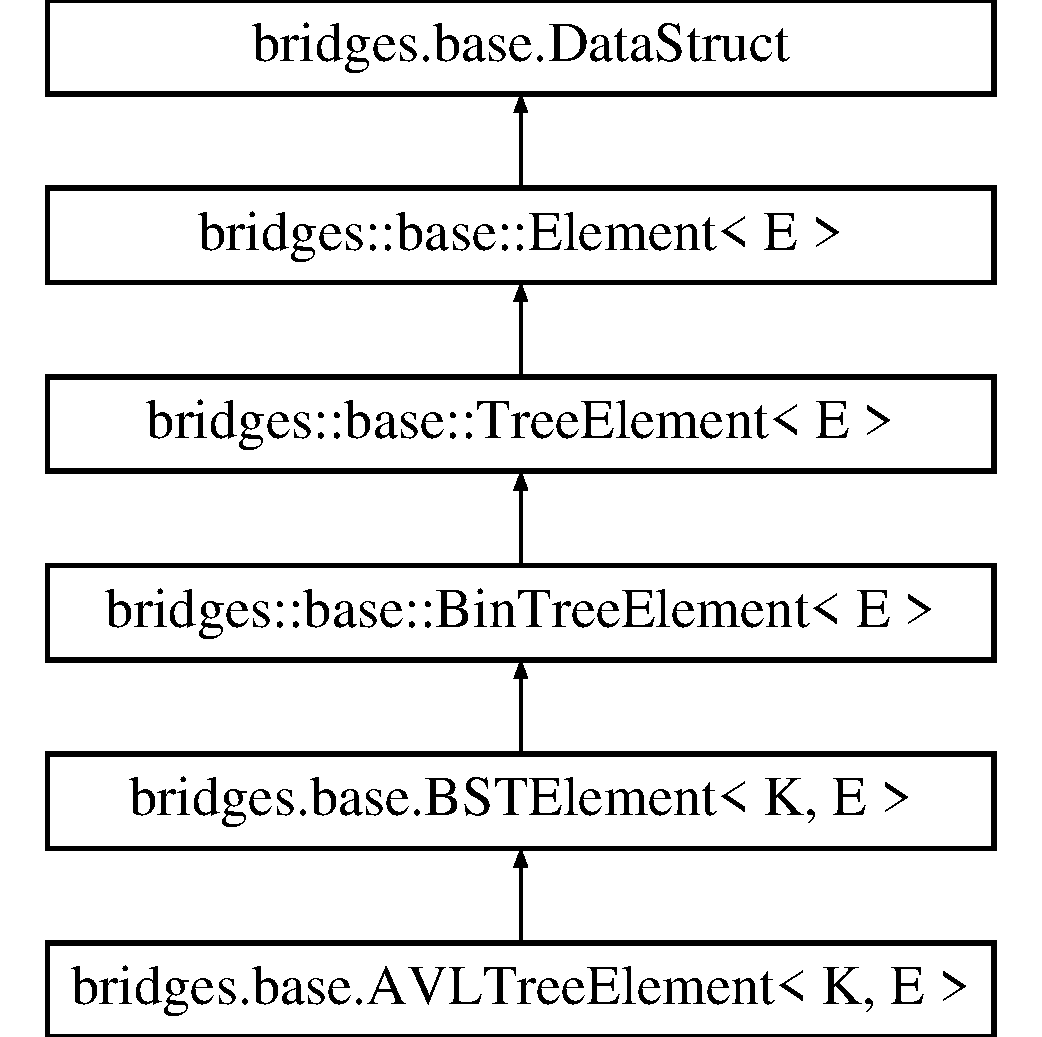
\includegraphics[height=6.000000cm]{classbridges_1_1base_1_1_b_s_t_element}
\end{center}
\end{figure}
\subsection*{Public Member Functions}
\begin{DoxyCompactItemize}
\item 
\mbox{\hyperlink{classbridges_1_1base_1_1_b_s_t_element_a5a557bf3e29e2936c244147c69e04795}{B\+S\+T\+Element}} ()
\item 
\mbox{\hyperlink{classbridges_1_1base_1_1_b_s_t_element_a0ec94ad6e2313ada05b48eb83a2f31cb}{B\+S\+T\+Element}} (E e, \mbox{\hyperlink{classbridges_1_1base_1_1_b_s_t_element}{B\+S\+T\+Element}}$<$ K, E $>$ left, \mbox{\hyperlink{classbridges_1_1base_1_1_b_s_t_element}{B\+S\+T\+Element}}$<$ K, E $>$ right)
\item 
\mbox{\hyperlink{classbridges_1_1base_1_1_b_s_t_element_a6b5bae96b241996942c467a78e6262ea}{B\+S\+T\+Element}} (K key, E e, \mbox{\hyperlink{classbridges_1_1base_1_1_b_s_t_element}{B\+S\+T\+Element}}$<$ K, E $>$ left, \mbox{\hyperlink{classbridges_1_1base_1_1_b_s_t_element}{B\+S\+T\+Element}}$<$ K, E $>$ right)
\item 
\mbox{\hyperlink{classbridges_1_1base_1_1_b_s_t_element_aa40760e586322a406841765bcf2aafc6}{B\+S\+T\+Element}} (E e)
\item 
String \mbox{\hyperlink{classbridges_1_1base_1_1_b_s_t_element_ae51e96c80d61e1a6c74f6d56a4bc2fef}{get\+Data\+Struct\+Type}} ()
\item 
\mbox{\hyperlink{classbridges_1_1base_1_1_b_s_t_element_ae19a9a445ae112673edf57a24dcf38e9}{B\+S\+T\+Element}} (K key, E e)
\item 
\mbox{\hyperlink{classbridges_1_1base_1_1_b_s_t_element_ab4a92ca5d5bdd5966bd63def8e867173}{B\+S\+T\+Element}} (String label, E e)
\item 
\mbox{\hyperlink{classbridges_1_1base_1_1_b_s_t_element_a6b76778c0c1486f599b90e51cf0a477c}{B\+S\+T\+Element}} (String label, K key, E e)
\item 
\mbox{\hyperlink{classbridges_1_1base_1_1_b_s_t_element_a067f0fcc18228e8c9427deadba9f4d96}{B\+S\+T\+Element}} (\mbox{\hyperlink{classbridges_1_1base_1_1_b_s_t_element}{B\+S\+T\+Element}}$<$ K, E $>$ left, \mbox{\hyperlink{classbridges_1_1base_1_1_b_s_t_element}{B\+S\+T\+Element}}$<$ K, E $>$ right)
\item 
K \mbox{\hyperlink{classbridges_1_1base_1_1_b_s_t_element_afba950fad36d3327b01003df3ba4cc9f}{get\+Key}} ()
\item 
void \mbox{\hyperlink{classbridges_1_1base_1_1_b_s_t_element_a51990b684df6998dc25b324dc7631ab4}{set\+Key}} (K key)
\item 
\mbox{\hyperlink{classbridges_1_1base_1_1_b_s_t_element}{B\+S\+T\+Element}}$<$ K, E $>$ \mbox{\hyperlink{classbridges_1_1base_1_1_b_s_t_element_a8abdd6e4a0486de7fa45fbb233b56688}{get\+Left}} ()
\item 
\mbox{\hyperlink{classbridges_1_1base_1_1_b_s_t_element}{B\+S\+T\+Element}}$<$ K, E $>$ \mbox{\hyperlink{classbridges_1_1base_1_1_b_s_t_element_ae7ed1b98f48acfcfc0a3a5bf6219ce00}{get\+Right}} ()
\end{DoxyCompactItemize}
\subsection*{Additional Inherited Members}


\subsection{Detailed Description}
The \mbox{\hyperlink{classbridges_1_1base_1_1_b_s_t_element}{B\+S\+T\+Element}} class is the building block for creating binary search trees. 

The \mbox{\hyperlink{classbridges_1_1base_1_1_b_s_t_element}{B\+S\+T\+Element}} class is the building block for creating binary search tree structures. It contains two children (viz., left, right), and a search key, to be used in search operations .

\mbox{\hyperlink{classbridges_1_1base_1_1_b_s_t_element}{B\+S\+T\+Element}} contains a visualizer (\mbox{\hyperlink{classbridges_1_1base_1_1_element_visualizer}{Element\+Visualizer}}) object for setting visual attributes (color, shape, opacity, size), necessary for displaying them in a web browser.

B\+ST Elements also have a \mbox{\hyperlink{classbridges_1_1base_1_1_link_visualizer}{Link\+Visualizer}} object, that is used when they are linked to another element, appropriate for setting link attributes, for instance, between the current element and its left or right child


\begin{DoxyParams}{Parameters}
{\em E} & he generic parameter object that is part of this element, representing application specific data. \\
\hline
{\em K} & is the search key parameter in the B\+ST node; K must be orderable, such as integer, float, string, etc., on which relational operators work.\\
\hline
\end{DoxyParams}
\begin{DoxyAuthor}{Author}
Kalpathi Subramanian, Mihai Mehedint
\end{DoxyAuthor}
\begin{DoxyDate}{Date}
6/22/16, 1/7/17, 5/17/17
\end{DoxyDate}
This class extends the \mbox{\hyperlink{classbridges_1_1base_1_1_bin_tree_element}{Bin\+Tree\+Element}} class by adding a \textquotesingle{}key\textquotesingle{} value for use in a binary search tree implementations.

\begin{DoxySeeAlso}{See also}
Example tutorial using \mbox{\hyperlink{classbridges_1_1base_1_1_b_s_t_element}{B\+S\+T\+Element}} at ~\newline
 \href{http://bridgesuncc.github.io/Hello_World_Tutorials/BST.html}{\tt http\+://bridgesuncc.\+github.\+io/\+Hello\+\_\+\+World\+\_\+\+Tutorials/\+B\+S\+T.\+html} 
\end{DoxySeeAlso}


\subsection{Constructor \& Destructor Documentation}
\mbox{\Hypertarget{classbridges_1_1base_1_1_b_s_t_element_a5a557bf3e29e2936c244147c69e04795}\label{classbridges_1_1base_1_1_b_s_t_element_a5a557bf3e29e2936c244147c69e04795}} 
\index{bridges\+::base\+::\+B\+S\+T\+Element@{bridges\+::base\+::\+B\+S\+T\+Element}!B\+S\+T\+Element@{B\+S\+T\+Element}}
\index{B\+S\+T\+Element@{B\+S\+T\+Element}!bridges\+::base\+::\+B\+S\+T\+Element@{bridges\+::base\+::\+B\+S\+T\+Element}}
\subsubsection{\texorpdfstring{B\+S\+T\+Element()}{BSTElement()}\hspace{0.1cm}{\footnotesize\ttfamily [1/8]}}
{\footnotesize\ttfamily \mbox{\hyperlink{classbridges_1_1base_1_1_b_s_t_element}{bridges.\+base.\+B\+S\+T\+Element}}$<$ K, E $>$.\mbox{\hyperlink{classbridges_1_1base_1_1_b_s_t_element}{B\+S\+T\+Element}} (\begin{DoxyParamCaption}{ }\end{DoxyParamCaption})}

Construct an empty \mbox{\hyperlink{classbridges_1_1base_1_1_b_s_t_element}{B\+S\+T\+Element}} with no key assigned and left and right pointers set to null. \mbox{\Hypertarget{classbridges_1_1base_1_1_b_s_t_element_a0ec94ad6e2313ada05b48eb83a2f31cb}\label{classbridges_1_1base_1_1_b_s_t_element_a0ec94ad6e2313ada05b48eb83a2f31cb}} 
\index{bridges\+::base\+::\+B\+S\+T\+Element@{bridges\+::base\+::\+B\+S\+T\+Element}!B\+S\+T\+Element@{B\+S\+T\+Element}}
\index{B\+S\+T\+Element@{B\+S\+T\+Element}!bridges\+::base\+::\+B\+S\+T\+Element@{bridges\+::base\+::\+B\+S\+T\+Element}}
\subsubsection{\texorpdfstring{B\+S\+T\+Element()}{BSTElement()}\hspace{0.1cm}{\footnotesize\ttfamily [2/8]}}
{\footnotesize\ttfamily \mbox{\hyperlink{classbridges_1_1base_1_1_b_s_t_element}{bridges.\+base.\+B\+S\+T\+Element}}$<$ K, E $>$.\mbox{\hyperlink{classbridges_1_1base_1_1_b_s_t_element}{B\+S\+T\+Element}} (\begin{DoxyParamCaption}\item[{E}]{e,  }\item[{\mbox{\hyperlink{classbridges_1_1base_1_1_b_s_t_element}{B\+S\+T\+Element}}$<$ K, E $>$}]{left,  }\item[{\mbox{\hyperlink{classbridges_1_1base_1_1_b_s_t_element}{B\+S\+T\+Element}}$<$ K, E $>$}]{right }\end{DoxyParamCaption})}

Construct a \mbox{\hyperlink{classbridges_1_1base_1_1_b_s_t_element}{B\+S\+T\+Element}} holding an object \char`\"{}e\char`\"{} with a left pointer assigned to \char`\"{}left\char`\"{} and a right pointer assigned to \char`\"{}right\char`\"{}. 
\begin{DoxyParams}{Parameters}
{\em e} & the object that \mbox{\hyperlink{classbridges_1_1base_1_1_b_s_t_element}{B\+S\+T\+Element}} is holding \\
\hline
{\em left} & the \mbox{\hyperlink{classbridges_1_1base_1_1_b_s_t_element}{B\+S\+T\+Element}} that should be assigned to the left pointer \\
\hline
{\em right} & the B\+S\+T\+Elemetn taht should be assigned to the right pointer \\
\hline
\end{DoxyParams}
\mbox{\Hypertarget{classbridges_1_1base_1_1_b_s_t_element_a6b5bae96b241996942c467a78e6262ea}\label{classbridges_1_1base_1_1_b_s_t_element_a6b5bae96b241996942c467a78e6262ea}} 
\index{bridges\+::base\+::\+B\+S\+T\+Element@{bridges\+::base\+::\+B\+S\+T\+Element}!B\+S\+T\+Element@{B\+S\+T\+Element}}
\index{B\+S\+T\+Element@{B\+S\+T\+Element}!bridges\+::base\+::\+B\+S\+T\+Element@{bridges\+::base\+::\+B\+S\+T\+Element}}
\subsubsection{\texorpdfstring{B\+S\+T\+Element()}{BSTElement()}\hspace{0.1cm}{\footnotesize\ttfamily [3/8]}}
{\footnotesize\ttfamily \mbox{\hyperlink{classbridges_1_1base_1_1_b_s_t_element}{bridges.\+base.\+B\+S\+T\+Element}}$<$ K, E $>$.\mbox{\hyperlink{classbridges_1_1base_1_1_b_s_t_element}{B\+S\+T\+Element}} (\begin{DoxyParamCaption}\item[{K}]{key,  }\item[{E}]{e,  }\item[{\mbox{\hyperlink{classbridges_1_1base_1_1_b_s_t_element}{B\+S\+T\+Element}}$<$ K, E $>$}]{left,  }\item[{\mbox{\hyperlink{classbridges_1_1base_1_1_b_s_t_element}{B\+S\+T\+Element}}$<$ K, E $>$}]{right }\end{DoxyParamCaption})}

Construct a \mbox{\hyperlink{classbridges_1_1base_1_1_b_s_t_element}{B\+S\+T\+Element}} with a key \char`\"{}key\char`\"{}, holding an object \char`\"{}e\char`\"{} with a left pointer assigned to \char`\"{}left\char`\"{} and a right pointer assigned to \char`\"{}right\char`\"{}.


\begin{DoxyParams}{Parameters}
{\em key} & the key to be used in a binary search tree implementation \\
\hline
{\em e} & the object this \mbox{\hyperlink{classbridges_1_1base_1_1_b_s_t_element}{B\+S\+T\+Element}} is holding \\
\hline
{\em left} & the \mbox{\hyperlink{classbridges_1_1base_1_1_b_s_t_element}{B\+S\+T\+Element}} that should be assigned to the left pointer \\
\hline
{\em right} & the \mbox{\hyperlink{classbridges_1_1base_1_1_b_s_t_element}{B\+S\+T\+Element}} that should be assigned to the right pointer \\
\hline
\end{DoxyParams}
\mbox{\Hypertarget{classbridges_1_1base_1_1_b_s_t_element_aa40760e586322a406841765bcf2aafc6}\label{classbridges_1_1base_1_1_b_s_t_element_aa40760e586322a406841765bcf2aafc6}} 
\index{bridges\+::base\+::\+B\+S\+T\+Element@{bridges\+::base\+::\+B\+S\+T\+Element}!B\+S\+T\+Element@{B\+S\+T\+Element}}
\index{B\+S\+T\+Element@{B\+S\+T\+Element}!bridges\+::base\+::\+B\+S\+T\+Element@{bridges\+::base\+::\+B\+S\+T\+Element}}
\subsubsection{\texorpdfstring{B\+S\+T\+Element()}{BSTElement()}\hspace{0.1cm}{\footnotesize\ttfamily [4/8]}}
{\footnotesize\ttfamily \mbox{\hyperlink{classbridges_1_1base_1_1_b_s_t_element}{bridges.\+base.\+B\+S\+T\+Element}}$<$ K, E $>$.\mbox{\hyperlink{classbridges_1_1base_1_1_b_s_t_element}{B\+S\+T\+Element}} (\begin{DoxyParamCaption}\item[{E}]{e }\end{DoxyParamCaption})}

Construct a \mbox{\hyperlink{classbridges_1_1base_1_1_b_s_t_element}{B\+S\+T\+Element}} holding the object \char`\"{}e\char`\"{}, with no key assigned and left and right pointers set to null.


\begin{DoxyParams}{Parameters}
{\em e} & the object this \mbox{\hyperlink{classbridges_1_1base_1_1_b_s_t_element}{B\+S\+T\+Element}} is holding \\
\hline
\end{DoxyParams}
\mbox{\Hypertarget{classbridges_1_1base_1_1_b_s_t_element_ae19a9a445ae112673edf57a24dcf38e9}\label{classbridges_1_1base_1_1_b_s_t_element_ae19a9a445ae112673edf57a24dcf38e9}} 
\index{bridges\+::base\+::\+B\+S\+T\+Element@{bridges\+::base\+::\+B\+S\+T\+Element}!B\+S\+T\+Element@{B\+S\+T\+Element}}
\index{B\+S\+T\+Element@{B\+S\+T\+Element}!bridges\+::base\+::\+B\+S\+T\+Element@{bridges\+::base\+::\+B\+S\+T\+Element}}
\subsubsection{\texorpdfstring{B\+S\+T\+Element()}{BSTElement()}\hspace{0.1cm}{\footnotesize\ttfamily [5/8]}}
{\footnotesize\ttfamily \mbox{\hyperlink{classbridges_1_1base_1_1_b_s_t_element}{bridges.\+base.\+B\+S\+T\+Element}}$<$ K, E $>$.\mbox{\hyperlink{classbridges_1_1base_1_1_b_s_t_element}{B\+S\+T\+Element}} (\begin{DoxyParamCaption}\item[{K}]{key,  }\item[{E}]{e }\end{DoxyParamCaption})}

Construct a \mbox{\hyperlink{classbridges_1_1base_1_1_b_s_t_element}{B\+S\+T\+Element}} holding the object \char`\"{}e\char`\"{}, with key \char`\"{}key\char`\"{} assigned and left and right pointers set to null. 
\begin{DoxyParams}{Parameters}
{\em key} & the key to be used in a binary search tree implementation \\
\hline
{\em e} & the object this \mbox{\hyperlink{classbridges_1_1base_1_1_b_s_t_element}{B\+S\+T\+Element}} is holding \\
\hline
\end{DoxyParams}
\mbox{\Hypertarget{classbridges_1_1base_1_1_b_s_t_element_ab4a92ca5d5bdd5966bd63def8e867173}\label{classbridges_1_1base_1_1_b_s_t_element_ab4a92ca5d5bdd5966bd63def8e867173}} 
\index{bridges\+::base\+::\+B\+S\+T\+Element@{bridges\+::base\+::\+B\+S\+T\+Element}!B\+S\+T\+Element@{B\+S\+T\+Element}}
\index{B\+S\+T\+Element@{B\+S\+T\+Element}!bridges\+::base\+::\+B\+S\+T\+Element@{bridges\+::base\+::\+B\+S\+T\+Element}}
\subsubsection{\texorpdfstring{B\+S\+T\+Element()}{BSTElement()}\hspace{0.1cm}{\footnotesize\ttfamily [6/8]}}
{\footnotesize\ttfamily \mbox{\hyperlink{classbridges_1_1base_1_1_b_s_t_element}{bridges.\+base.\+B\+S\+T\+Element}}$<$ K, E $>$.\mbox{\hyperlink{classbridges_1_1base_1_1_b_s_t_element}{B\+S\+T\+Element}} (\begin{DoxyParamCaption}\item[{String}]{label,  }\item[{E}]{e }\end{DoxyParamCaption})}

Construct a \mbox{\hyperlink{classbridges_1_1base_1_1_b_s_t_element}{B\+S\+T\+Element}} holding the object \char`\"{}e\char`\"{}, with label set to \char`\"{}label\char`\"{}, with no key assigned, and left and right pointers set to null. 
\begin{DoxyParams}{Parameters}
{\em label} & the label of \mbox{\hyperlink{classbridges_1_1base_1_1_b_s_t_element}{B\+S\+T\+Element}} that shows up on the Bridges visualization \\
\hline
{\em e} & the object this \mbox{\hyperlink{classbridges_1_1base_1_1_b_s_t_element}{B\+S\+T\+Element}} is holding \\
\hline
\end{DoxyParams}
\mbox{\Hypertarget{classbridges_1_1base_1_1_b_s_t_element_a6b76778c0c1486f599b90e51cf0a477c}\label{classbridges_1_1base_1_1_b_s_t_element_a6b76778c0c1486f599b90e51cf0a477c}} 
\index{bridges\+::base\+::\+B\+S\+T\+Element@{bridges\+::base\+::\+B\+S\+T\+Element}!B\+S\+T\+Element@{B\+S\+T\+Element}}
\index{B\+S\+T\+Element@{B\+S\+T\+Element}!bridges\+::base\+::\+B\+S\+T\+Element@{bridges\+::base\+::\+B\+S\+T\+Element}}
\subsubsection{\texorpdfstring{B\+S\+T\+Element()}{BSTElement()}\hspace{0.1cm}{\footnotesize\ttfamily [7/8]}}
{\footnotesize\ttfamily \mbox{\hyperlink{classbridges_1_1base_1_1_b_s_t_element}{bridges.\+base.\+B\+S\+T\+Element}}$<$ K, E $>$.\mbox{\hyperlink{classbridges_1_1base_1_1_b_s_t_element}{B\+S\+T\+Element}} (\begin{DoxyParamCaption}\item[{String}]{label,  }\item[{K}]{key,  }\item[{E}]{e }\end{DoxyParamCaption})}

Construct a \mbox{\hyperlink{classbridges_1_1base_1_1_b_s_t_element}{B\+S\+T\+Element}} holding the object \char`\"{}e\char`\"{}, with label set to \char`\"{}label\char`\"{}, with \char`\"{}key\char`\"{} assigned to key, and left and right pointers set to null.


\begin{DoxyParams}{Parameters}
{\em label} & the label of \mbox{\hyperlink{classbridges_1_1base_1_1_b_s_t_element}{B\+S\+T\+Element}} that shows up on the Bridges visualization \\
\hline
{\em key} & the key to be used in a binary search tree implementation \\
\hline
{\em e} & the object this \mbox{\hyperlink{classbridges_1_1base_1_1_b_s_t_element}{B\+S\+T\+Element}} is holding \\
\hline
\end{DoxyParams}
\mbox{\Hypertarget{classbridges_1_1base_1_1_b_s_t_element_a067f0fcc18228e8c9427deadba9f4d96}\label{classbridges_1_1base_1_1_b_s_t_element_a067f0fcc18228e8c9427deadba9f4d96}} 
\index{bridges\+::base\+::\+B\+S\+T\+Element@{bridges\+::base\+::\+B\+S\+T\+Element}!B\+S\+T\+Element@{B\+S\+T\+Element}}
\index{B\+S\+T\+Element@{B\+S\+T\+Element}!bridges\+::base\+::\+B\+S\+T\+Element@{bridges\+::base\+::\+B\+S\+T\+Element}}
\subsubsection{\texorpdfstring{B\+S\+T\+Element()}{BSTElement()}\hspace{0.1cm}{\footnotesize\ttfamily [8/8]}}
{\footnotesize\ttfamily \mbox{\hyperlink{classbridges_1_1base_1_1_b_s_t_element}{bridges.\+base.\+B\+S\+T\+Element}}$<$ K, E $>$.\mbox{\hyperlink{classbridges_1_1base_1_1_b_s_t_element}{B\+S\+T\+Element}} (\begin{DoxyParamCaption}\item[{\mbox{\hyperlink{classbridges_1_1base_1_1_b_s_t_element}{B\+S\+T\+Element}}$<$ K, E $>$}]{left,  }\item[{\mbox{\hyperlink{classbridges_1_1base_1_1_b_s_t_element}{B\+S\+T\+Element}}$<$ K, E $>$}]{right }\end{DoxyParamCaption})}

Construct an empty \mbox{\hyperlink{classbridges_1_1base_1_1_b_s_t_element}{B\+S\+T\+Element}}, with no key assigned, and left and right pointers set to null. 
\begin{DoxyParams}{Parameters}
{\em left} & the \mbox{\hyperlink{classbridges_1_1base_1_1_b_s_t_element}{B\+S\+T\+Element}} that should be assigned to the left pointer \\
\hline
{\em right} & the \mbox{\hyperlink{classbridges_1_1base_1_1_b_s_t_element}{B\+S\+T\+Element}} that should be assigned to the right pointer \\
\hline
\end{DoxyParams}


\subsection{Member Function Documentation}
\mbox{\Hypertarget{classbridges_1_1base_1_1_b_s_t_element_ae51e96c80d61e1a6c74f6d56a4bc2fef}\label{classbridges_1_1base_1_1_b_s_t_element_ae51e96c80d61e1a6c74f6d56a4bc2fef}} 
\index{bridges\+::base\+::\+B\+S\+T\+Element@{bridges\+::base\+::\+B\+S\+T\+Element}!get\+Data\+Struct\+Type@{get\+Data\+Struct\+Type}}
\index{get\+Data\+Struct\+Type@{get\+Data\+Struct\+Type}!bridges\+::base\+::\+B\+S\+T\+Element@{bridges\+::base\+::\+B\+S\+T\+Element}}
\subsubsection{\texorpdfstring{get\+Data\+Struct\+Type()}{getDataStructType()}}
{\footnotesize\ttfamily String \mbox{\hyperlink{classbridges_1_1base_1_1_b_s_t_element}{bridges.\+base.\+B\+S\+T\+Element}}$<$ K, E $>$.get\+Data\+Struct\+Type (\begin{DoxyParamCaption}{ }\end{DoxyParamCaption})}

This method gets the data structure type

\begin{DoxyReturn}{Returns}
The date structure type as a string 
\end{DoxyReturn}
\mbox{\Hypertarget{classbridges_1_1base_1_1_b_s_t_element_afba950fad36d3327b01003df3ba4cc9f}\label{classbridges_1_1base_1_1_b_s_t_element_afba950fad36d3327b01003df3ba4cc9f}} 
\index{bridges\+::base\+::\+B\+S\+T\+Element@{bridges\+::base\+::\+B\+S\+T\+Element}!get\+Key@{get\+Key}}
\index{get\+Key@{get\+Key}!bridges\+::base\+::\+B\+S\+T\+Element@{bridges\+::base\+::\+B\+S\+T\+Element}}
\subsubsection{\texorpdfstring{get\+Key()}{getKey()}}
{\footnotesize\ttfamily K \mbox{\hyperlink{classbridges_1_1base_1_1_b_s_t_element}{bridges.\+base.\+B\+S\+T\+Element}}$<$ K, E $>$.get\+Key (\begin{DoxyParamCaption}{ }\end{DoxyParamCaption})}

Return the key of the \mbox{\hyperlink{classbridges_1_1base_1_1_b_s_t_element}{B\+S\+T\+Element}}

\begin{DoxyReturn}{Returns}
the key of this \mbox{\hyperlink{classbridges_1_1base_1_1_b_s_t_element}{B\+S\+T\+Element}} 
\end{DoxyReturn}
\mbox{\Hypertarget{classbridges_1_1base_1_1_b_s_t_element_a8abdd6e4a0486de7fa45fbb233b56688}\label{classbridges_1_1base_1_1_b_s_t_element_a8abdd6e4a0486de7fa45fbb233b56688}} 
\index{bridges\+::base\+::\+B\+S\+T\+Element@{bridges\+::base\+::\+B\+S\+T\+Element}!get\+Left@{get\+Left}}
\index{get\+Left@{get\+Left}!bridges\+::base\+::\+B\+S\+T\+Element@{bridges\+::base\+::\+B\+S\+T\+Element}}
\subsubsection{\texorpdfstring{get\+Left()}{getLeft()}}
{\footnotesize\ttfamily \mbox{\hyperlink{classbridges_1_1base_1_1_b_s_t_element}{B\+S\+T\+Element}}$<$K, E$>$ \mbox{\hyperlink{classbridges_1_1base_1_1_b_s_t_element}{bridges.\+base.\+B\+S\+T\+Element}}$<$ K, E $>$.get\+Left (\begin{DoxyParamCaption}{ }\end{DoxyParamCaption})}

\mbox{\Hypertarget{classbridges_1_1base_1_1_b_s_t_element_ae7ed1b98f48acfcfc0a3a5bf6219ce00}\label{classbridges_1_1base_1_1_b_s_t_element_ae7ed1b98f48acfcfc0a3a5bf6219ce00}} 
\index{bridges\+::base\+::\+B\+S\+T\+Element@{bridges\+::base\+::\+B\+S\+T\+Element}!get\+Right@{get\+Right}}
\index{get\+Right@{get\+Right}!bridges\+::base\+::\+B\+S\+T\+Element@{bridges\+::base\+::\+B\+S\+T\+Element}}
\subsubsection{\texorpdfstring{get\+Right()}{getRight()}}
{\footnotesize\ttfamily \mbox{\hyperlink{classbridges_1_1base_1_1_b_s_t_element}{B\+S\+T\+Element}}$<$K, E$>$ \mbox{\hyperlink{classbridges_1_1base_1_1_b_s_t_element}{bridges.\+base.\+B\+S\+T\+Element}}$<$ K, E $>$.get\+Right (\begin{DoxyParamCaption}{ }\end{DoxyParamCaption})}

\mbox{\Hypertarget{classbridges_1_1base_1_1_b_s_t_element_a51990b684df6998dc25b324dc7631ab4}\label{classbridges_1_1base_1_1_b_s_t_element_a51990b684df6998dc25b324dc7631ab4}} 
\index{bridges\+::base\+::\+B\+S\+T\+Element@{bridges\+::base\+::\+B\+S\+T\+Element}!set\+Key@{set\+Key}}
\index{set\+Key@{set\+Key}!bridges\+::base\+::\+B\+S\+T\+Element@{bridges\+::base\+::\+B\+S\+T\+Element}}
\subsubsection{\texorpdfstring{set\+Key()}{setKey()}}
{\footnotesize\ttfamily void \mbox{\hyperlink{classbridges_1_1base_1_1_b_s_t_element}{bridges.\+base.\+B\+S\+T\+Element}}$<$ K, E $>$.set\+Key (\begin{DoxyParamCaption}\item[{K}]{key }\end{DoxyParamCaption})}

Set the key of the \mbox{\hyperlink{classbridges_1_1base_1_1_b_s_t_element}{B\+S\+T\+Element}} to key 
\begin{DoxyParams}{Parameters}
{\em key} & the key to set \\
\hline
\end{DoxyParams}


The documentation for this class was generated from the following file\+:\begin{DoxyCompactItemize}
\item 
/\+Users/kalpathi/gr/bridges/client/java/bridges-\/17/src/main/java/edu/uncc/cs/bridges\+\_\+v21/base/\mbox{\hyperlink{_b_s_t_element_8java}{B\+S\+T\+Element.\+java}}\end{DoxyCompactItemize}

\hypertarget{classbridges_1_1data__src__dependent_1_1_cancer_incidence}{}\section{bridges.\+data\+\_\+src\+\_\+dependent.\+Cancer\+Incidence Class Reference}
\label{classbridges_1_1data__src__dependent_1_1_cancer_incidence}\index{bridges.\+data\+\_\+src\+\_\+dependent.\+Cancer\+Incidence@{bridges.\+data\+\_\+src\+\_\+dependent.\+Cancer\+Incidence}}


Inherits bridges.\+data\+\_\+src\+\_\+dependent.\+Data\+Source.



\subsection{Detailed Description}
United States Cancer Statistics from the U.\+S. Center for Disease Control. 

From the United States Cancer Statistics as part of the U.\+S. Center for Disease Control, the following data set focuses on the crude rate for all types of cancer reported for different demograpic groups. Significant groupings include age, gender, race and geographical area.

\href{http://www.cdc.gov/cancer/npcr/uscs/download_data.htm}{\tt http\+://www.\+cdc.\+gov/cancer/npcr/uscs/download\+\_\+data.\+htm} Data\+: Courtesy of Corgis Datasets, 2017

Author\+: Kalpathi Subramanian, April, 2017 \subsection*{Public Member Functions}
\begin{DoxyCompactItemize}
\item 
\hyperlink{classbridges_1_1data__src__dependent_1_1_cancer_incidence_a92db1eb4292c77f07619019587caf5cc}{Cancer\+Incidence} ()
\item 
\hyperlink{classbridges_1_1data__src__dependent_1_1_cancer_incidence_a3db553c2769892563c3f1ebb033ba4c6}{Cancer\+Incidence} (String canc\+\_\+label)
\item 
String \hyperlink{classbridges_1_1data__src__dependent_1_1_cancer_incidence_ac7958f37807979cf06e712373f080b9a}{get\+Name} ()
\begin{DoxyCompactList}\small\item\em get the name of the incidence report. \end{DoxyCompactList}\item 
void \hyperlink{classbridges_1_1data__src__dependent_1_1_cancer_incidence_a1aef58b128adfd1e2a31ab9726247e9e}{set\+Name} (String name)
\begin{DoxyCompactList}\small\item\em sets the string name \end{DoxyCompactList}\item 
double \hyperlink{classbridges_1_1data__src__dependent_1_1_cancer_incidence_a87bc1cbc5a72eb9b4df5ff7ab4843ae8}{get\+Age\+Adjusted\+Rate} ()
\item 
void \hyperlink{classbridges_1_1data__src__dependent_1_1_cancer_incidence_a26c2d63e8465bcfdab047129312b4897}{set\+Age\+Adjusted\+Rate} (double aar)
\begin{DoxyCompactList}\small\item\em Set age adjusted cancer rate. \end{DoxyCompactList}\item 
double \hyperlink{classbridges_1_1data__src__dependent_1_1_cancer_incidence_a7e5dab6d140f2a8e162c5d5c514c74c1}{get\+Age\+Adjusted\+C\+I\+\_\+\+Lower} ()
\item 
void \hyperlink{classbridges_1_1data__src__dependent_1_1_cancer_incidence_a4cd8ce7c68f00d2cd15928764cc32c09}{set\+Age\+Adjusted\+C\+I\+\_\+\+Lower} (double ci\+\_\+l)
\begin{DoxyCompactList}\small\item\em Set age adjusted cancer conf interval (lower) \end{DoxyCompactList}\item 
double \hyperlink{classbridges_1_1data__src__dependent_1_1_cancer_incidence_ae7b71d91c3acae9fce3536f6a9d8362b}{get\+Age\+Adjusted\+C\+I\+\_\+\+Upper} ()
\item 
void \hyperlink{classbridges_1_1data__src__dependent_1_1_cancer_incidence_aeb386486bfbd96ba9ab689b7d95d4522}{set\+Age\+Adjusted\+C\+I\+\_\+\+Upper} (double ci\+\_\+u)
\begin{DoxyCompactList}\small\item\em Set age adjusted cancer conf interval (upper) \end{DoxyCompactList}\item 
double \hyperlink{classbridges_1_1data__src__dependent_1_1_cancer_incidence_afc2ddb3099dffc46371ad7188278501d}{get\+Crude\+Rate} ()
\begin{DoxyCompactList}\small\item\em Get the cancer rate, adjusted for population. \end{DoxyCompactList}\item 
void \hyperlink{classbridges_1_1data__src__dependent_1_1_cancer_incidence_a64a737fd7481262650efd596c508ffd6}{set\+Crude\+Rate} (double cr)
\begin{DoxyCompactList}\small\item\em Set cancer rate, adjusted for population. \end{DoxyCompactList}\item 
double \hyperlink{classbridges_1_1data__src__dependent_1_1_cancer_incidence_a8c410730b03abc78395e75b5024d495e}{get\+Crude\+Rate\+\_\+\+C\+I\+\_\+\+Lower} ()
\begin{DoxyCompactList}\small\item\em Get the expected cancer crude rate confidence interval(lower), adjusted for age of participants. \end{DoxyCompactList}\item 
void \hyperlink{classbridges_1_1data__src__dependent_1_1_cancer_incidence_a72e3960af58f32d26e32f49ada2f1555}{set\+Crude\+Rate\+\_\+\+C\+I\+\_\+\+Lower} (double cr\+\_\+l)
\begin{DoxyCompactList}\small\item\em Set age adjusted cancer crude conf interval (lower) \end{DoxyCompactList}\item 
double \hyperlink{classbridges_1_1data__src__dependent_1_1_cancer_incidence_a4ca1ceed275ab6371f861d3a03975f15}{get\+Crude\+Rate\+\_\+\+C\+I\+\_\+\+Upper} ()
\item 
void \hyperlink{classbridges_1_1data__src__dependent_1_1_cancer_incidence_a99e25dd53093badf350b06b7e0c8b725}{set\+Crude\+Rate\+\_\+\+C\+I\+\_\+\+Upper} (double cr\+\_\+u)
\begin{DoxyCompactList}\small\item\em Set crude rate CI (upper) \end{DoxyCompactList}\item 
int \hyperlink{classbridges_1_1data__src__dependent_1_1_cancer_incidence_aaff714019154afa796d54ed57ffc9492}{get\+Year} ()
\begin{DoxyCompactList}\small\item\em Get the year of this cancer record. \end{DoxyCompactList}\item 
void \hyperlink{classbridges_1_1data__src__dependent_1_1_cancer_incidence_aa5524736b76d67f1248d1a05d9f596a9}{set\+Year} (int y)
\begin{DoxyCompactList}\small\item\em Set the year of this cancer record. \end{DoxyCompactList}\item 
String \hyperlink{classbridges_1_1data__src__dependent_1_1_cancer_incidence_a2c3cbe65d89827c167f15314b8b088b3}{get\+Gender} ()
\item 
void \hyperlink{classbridges_1_1data__src__dependent_1_1_cancer_incidence_a217681578e13197e1d177932c73ea80f}{set\+Gender} (String g)
\begin{DoxyCompactList}\small\item\em Set gender. \end{DoxyCompactList}\item 
String \hyperlink{classbridges_1_1data__src__dependent_1_1_cancer_incidence_a18de1c14d36cd7656555c8465ea8a009}{get\+Race} ()
\item 
void \hyperlink{classbridges_1_1data__src__dependent_1_1_cancer_incidence_a8c26c4358561453f3d2ca3a463eed872}{set\+Race} (String r)
\begin{DoxyCompactList}\small\item\em Set race. \end{DoxyCompactList}\item 
String \hyperlink{classbridges_1_1data__src__dependent_1_1_cancer_incidence_a844c6c3317bdb6b124f32b40804e1ff7}{get\+Event\+Type} ()
\begin{DoxyCompactList}\small\item\em Get the event type (incidence, mortality, etc) \end{DoxyCompactList}\item 
void \hyperlink{classbridges_1_1data__src__dependent_1_1_cancer_incidence_a39338b20223e60b79fa38b3034ca46b7}{set\+Event\+Type} (String et)
\begin{DoxyCompactList}\small\item\em Set event type. \end{DoxyCompactList}\item 
int \hyperlink{classbridges_1_1data__src__dependent_1_1_cancer_incidence_a41c2507d46589080f6bb76ab29f53665}{get\+Population} ()
\begin{DoxyCompactList}\small\item\em Get the population size. \end{DoxyCompactList}\item 
void \hyperlink{classbridges_1_1data__src__dependent_1_1_cancer_incidence_a9f1caf002b6573aa699a81ed1b835af0}{set\+Population} (int pop)
\begin{DoxyCompactList}\small\item\em Set population size. \end{DoxyCompactList}\item 
String \hyperlink{classbridges_1_1data__src__dependent_1_1_cancer_incidence_ad4c0c709fa5da9c0f20b648052db5f26}{get\+Affected\+Area} ()
\begin{DoxyCompactList}\small\item\em Get the cancer incidence area (state, region, etc) \end{DoxyCompactList}\item 
void \hyperlink{classbridges_1_1data__src__dependent_1_1_cancer_incidence_a9c7f2d303da9498e5e6145439c5a6fbc}{set\+Affected\+Area} (String area)
\begin{DoxyCompactList}\small\item\em Set cancer incidence area. \end{DoxyCompactList}\item 
int \hyperlink{classbridges_1_1data__src__dependent_1_1_cancer_incidence_a8769cb18ddb590dc41a04a220174f3df}{get\+Count} ()
\begin{DoxyCompactList}\small\item\em Get the number of people affected in this group. \end{DoxyCompactList}\item 
void \hyperlink{classbridges_1_1data__src__dependent_1_1_cancer_incidence_a18099439ef6e35cf240b06f0e0158c72}{set\+Count} (int c)
\begin{DoxyCompactList}\small\item\em Set cancer incidence count. \end{DoxyCompactList}\item 
double \hyperlink{classbridges_1_1data__src__dependent_1_1_cancer_incidence_a24aa8144dcacd93a26c3c033471666df}{get\+LocationX} ()
\begin{DoxyCompactList}\small\item\em Get the X coordinate of location. \end{DoxyCompactList}\item 
void \hyperlink{classbridges_1_1data__src__dependent_1_1_cancer_incidence_a384149c413173fba51adad1b1769797a}{set\+LocationX} (double locX)
\begin{DoxyCompactList}\small\item\em Set location (X coord) \end{DoxyCompactList}\item 
double \hyperlink{classbridges_1_1data__src__dependent_1_1_cancer_incidence_a53b56a9931a1d02ee356c6258e245aa8}{get\+LocationY} ()
\begin{DoxyCompactList}\small\item\em Get the Y coordinate of location. \end{DoxyCompactList}\item 
void \hyperlink{classbridges_1_1data__src__dependent_1_1_cancer_incidence_a14c6921a71834c14d561bc7f2aa8a18e}{set\+LocationY} (double locY)
\begin{DoxyCompactList}\small\item\em Set location (Y coord) \end{DoxyCompactList}\end{DoxyCompactItemize}


\subsection{Constructor \& Destructor Documentation}
\mbox{\Hypertarget{classbridges_1_1data__src__dependent_1_1_cancer_incidence_a92db1eb4292c77f07619019587caf5cc}\label{classbridges_1_1data__src__dependent_1_1_cancer_incidence_a92db1eb4292c77f07619019587caf5cc}} 
\index{bridges\+::data\+\_\+src\+\_\+dependent\+::\+Cancer\+Incidence@{bridges\+::data\+\_\+src\+\_\+dependent\+::\+Cancer\+Incidence}!Cancer\+Incidence@{Cancer\+Incidence}}
\index{Cancer\+Incidence@{Cancer\+Incidence}!bridges\+::data\+\_\+src\+\_\+dependent\+::\+Cancer\+Incidence@{bridges\+::data\+\_\+src\+\_\+dependent\+::\+Cancer\+Incidence}}
\subsubsection{\texorpdfstring{Cancer\+Incidence()}{CancerIncidence()}\hspace{0.1cm}{\footnotesize\ttfamily [1/2]}}
{\footnotesize\ttfamily bridges.\+data\+\_\+src\+\_\+dependent.\+Cancer\+Incidence.\+Cancer\+Incidence (\begin{DoxyParamCaption}{ }\end{DoxyParamCaption})}

\mbox{\Hypertarget{classbridges_1_1data__src__dependent_1_1_cancer_incidence_a3db553c2769892563c3f1ebb033ba4c6}\label{classbridges_1_1data__src__dependent_1_1_cancer_incidence_a3db553c2769892563c3f1ebb033ba4c6}} 
\index{bridges\+::data\+\_\+src\+\_\+dependent\+::\+Cancer\+Incidence@{bridges\+::data\+\_\+src\+\_\+dependent\+::\+Cancer\+Incidence}!Cancer\+Incidence@{Cancer\+Incidence}}
\index{Cancer\+Incidence@{Cancer\+Incidence}!bridges\+::data\+\_\+src\+\_\+dependent\+::\+Cancer\+Incidence@{bridges\+::data\+\_\+src\+\_\+dependent\+::\+Cancer\+Incidence}}
\subsubsection{\texorpdfstring{Cancer\+Incidence()}{CancerIncidence()}\hspace{0.1cm}{\footnotesize\ttfamily [2/2]}}
{\footnotesize\ttfamily bridges.\+data\+\_\+src\+\_\+dependent.\+Cancer\+Incidence.\+Cancer\+Incidence (\begin{DoxyParamCaption}\item[{String}]{canc\+\_\+label }\end{DoxyParamCaption})}



\subsection{Member Function Documentation}
\mbox{\Hypertarget{classbridges_1_1data__src__dependent_1_1_cancer_incidence_ad4c0c709fa5da9c0f20b648052db5f26}\label{classbridges_1_1data__src__dependent_1_1_cancer_incidence_ad4c0c709fa5da9c0f20b648052db5f26}} 
\index{bridges\+::data\+\_\+src\+\_\+dependent\+::\+Cancer\+Incidence@{bridges\+::data\+\_\+src\+\_\+dependent\+::\+Cancer\+Incidence}!get\+Affected\+Area@{get\+Affected\+Area}}
\index{get\+Affected\+Area@{get\+Affected\+Area}!bridges\+::data\+\_\+src\+\_\+dependent\+::\+Cancer\+Incidence@{bridges\+::data\+\_\+src\+\_\+dependent\+::\+Cancer\+Incidence}}
\subsubsection{\texorpdfstring{get\+Affected\+Area()}{getAffectedArea()}}
{\footnotesize\ttfamily String bridges.\+data\+\_\+src\+\_\+dependent.\+Cancer\+Incidence.\+get\+Affected\+Area (\begin{DoxyParamCaption}{ }\end{DoxyParamCaption})}



Get the cancer incidence area (state, region, etc) 

\begin{DoxyReturn}{Returns}
affected area 
\end{DoxyReturn}
\mbox{\Hypertarget{classbridges_1_1data__src__dependent_1_1_cancer_incidence_a7e5dab6d140f2a8e162c5d5c514c74c1}\label{classbridges_1_1data__src__dependent_1_1_cancer_incidence_a7e5dab6d140f2a8e162c5d5c514c74c1}} 
\index{bridges\+::data\+\_\+src\+\_\+dependent\+::\+Cancer\+Incidence@{bridges\+::data\+\_\+src\+\_\+dependent\+::\+Cancer\+Incidence}!get\+Age\+Adjusted\+C\+I\+\_\+\+Lower@{get\+Age\+Adjusted\+C\+I\+\_\+\+Lower}}
\index{get\+Age\+Adjusted\+C\+I\+\_\+\+Lower@{get\+Age\+Adjusted\+C\+I\+\_\+\+Lower}!bridges\+::data\+\_\+src\+\_\+dependent\+::\+Cancer\+Incidence@{bridges\+::data\+\_\+src\+\_\+dependent\+::\+Cancer\+Incidence}}
\subsubsection{\texorpdfstring{get\+Age\+Adjusted\+C\+I\+\_\+\+Lower()}{getAgeAdjustedCI\_Lower()}}
{\footnotesize\ttfamily double bridges.\+data\+\_\+src\+\_\+dependent.\+Cancer\+Incidence.\+get\+Age\+Adjusted\+C\+I\+\_\+\+Lower (\begin{DoxyParamCaption}{ }\end{DoxyParamCaption})}

\mbox{\Hypertarget{classbridges_1_1data__src__dependent_1_1_cancer_incidence_ae7b71d91c3acae9fce3536f6a9d8362b}\label{classbridges_1_1data__src__dependent_1_1_cancer_incidence_ae7b71d91c3acae9fce3536f6a9d8362b}} 
\index{bridges\+::data\+\_\+src\+\_\+dependent\+::\+Cancer\+Incidence@{bridges\+::data\+\_\+src\+\_\+dependent\+::\+Cancer\+Incidence}!get\+Age\+Adjusted\+C\+I\+\_\+\+Upper@{get\+Age\+Adjusted\+C\+I\+\_\+\+Upper}}
\index{get\+Age\+Adjusted\+C\+I\+\_\+\+Upper@{get\+Age\+Adjusted\+C\+I\+\_\+\+Upper}!bridges\+::data\+\_\+src\+\_\+dependent\+::\+Cancer\+Incidence@{bridges\+::data\+\_\+src\+\_\+dependent\+::\+Cancer\+Incidence}}
\subsubsection{\texorpdfstring{get\+Age\+Adjusted\+C\+I\+\_\+\+Upper()}{getAgeAdjustedCI\_Upper()}}
{\footnotesize\ttfamily double bridges.\+data\+\_\+src\+\_\+dependent.\+Cancer\+Incidence.\+get\+Age\+Adjusted\+C\+I\+\_\+\+Upper (\begin{DoxyParamCaption}{ }\end{DoxyParamCaption})}

\mbox{\Hypertarget{classbridges_1_1data__src__dependent_1_1_cancer_incidence_a87bc1cbc5a72eb9b4df5ff7ab4843ae8}\label{classbridges_1_1data__src__dependent_1_1_cancer_incidence_a87bc1cbc5a72eb9b4df5ff7ab4843ae8}} 
\index{bridges\+::data\+\_\+src\+\_\+dependent\+::\+Cancer\+Incidence@{bridges\+::data\+\_\+src\+\_\+dependent\+::\+Cancer\+Incidence}!get\+Age\+Adjusted\+Rate@{get\+Age\+Adjusted\+Rate}}
\index{get\+Age\+Adjusted\+Rate@{get\+Age\+Adjusted\+Rate}!bridges\+::data\+\_\+src\+\_\+dependent\+::\+Cancer\+Incidence@{bridges\+::data\+\_\+src\+\_\+dependent\+::\+Cancer\+Incidence}}
\subsubsection{\texorpdfstring{get\+Age\+Adjusted\+Rate()}{getAgeAdjustedRate()}}
{\footnotesize\ttfamily double bridges.\+data\+\_\+src\+\_\+dependent.\+Cancer\+Incidence.\+get\+Age\+Adjusted\+Rate (\begin{DoxyParamCaption}{ }\end{DoxyParamCaption})}

\mbox{\Hypertarget{classbridges_1_1data__src__dependent_1_1_cancer_incidence_a8769cb18ddb590dc41a04a220174f3df}\label{classbridges_1_1data__src__dependent_1_1_cancer_incidence_a8769cb18ddb590dc41a04a220174f3df}} 
\index{bridges\+::data\+\_\+src\+\_\+dependent\+::\+Cancer\+Incidence@{bridges\+::data\+\_\+src\+\_\+dependent\+::\+Cancer\+Incidence}!get\+Count@{get\+Count}}
\index{get\+Count@{get\+Count}!bridges\+::data\+\_\+src\+\_\+dependent\+::\+Cancer\+Incidence@{bridges\+::data\+\_\+src\+\_\+dependent\+::\+Cancer\+Incidence}}
\subsubsection{\texorpdfstring{get\+Count()}{getCount()}}
{\footnotesize\ttfamily int bridges.\+data\+\_\+src\+\_\+dependent.\+Cancer\+Incidence.\+get\+Count (\begin{DoxyParamCaption}{ }\end{DoxyParamCaption})}



Get the number of people affected in this group. 

\begin{DoxyReturn}{Returns}
number of people affected in this group. 
\end{DoxyReturn}
\mbox{\Hypertarget{classbridges_1_1data__src__dependent_1_1_cancer_incidence_afc2ddb3099dffc46371ad7188278501d}\label{classbridges_1_1data__src__dependent_1_1_cancer_incidence_afc2ddb3099dffc46371ad7188278501d}} 
\index{bridges\+::data\+\_\+src\+\_\+dependent\+::\+Cancer\+Incidence@{bridges\+::data\+\_\+src\+\_\+dependent\+::\+Cancer\+Incidence}!get\+Crude\+Rate@{get\+Crude\+Rate}}
\index{get\+Crude\+Rate@{get\+Crude\+Rate}!bridges\+::data\+\_\+src\+\_\+dependent\+::\+Cancer\+Incidence@{bridges\+::data\+\_\+src\+\_\+dependent\+::\+Cancer\+Incidence}}
\subsubsection{\texorpdfstring{get\+Crude\+Rate()}{getCrudeRate()}}
{\footnotesize\ttfamily double bridges.\+data\+\_\+src\+\_\+dependent.\+Cancer\+Incidence.\+get\+Crude\+Rate (\begin{DoxyParamCaption}{ }\end{DoxyParamCaption})}



Get the cancer rate, adjusted for population. 

\begin{DoxyReturn}{Returns}
crude cancer rate 
\end{DoxyReturn}
\mbox{\Hypertarget{classbridges_1_1data__src__dependent_1_1_cancer_incidence_a8c410730b03abc78395e75b5024d495e}\label{classbridges_1_1data__src__dependent_1_1_cancer_incidence_a8c410730b03abc78395e75b5024d495e}} 
\index{bridges\+::data\+\_\+src\+\_\+dependent\+::\+Cancer\+Incidence@{bridges\+::data\+\_\+src\+\_\+dependent\+::\+Cancer\+Incidence}!get\+Crude\+Rate\+\_\+\+C\+I\+\_\+\+Lower@{get\+Crude\+Rate\+\_\+\+C\+I\+\_\+\+Lower}}
\index{get\+Crude\+Rate\+\_\+\+C\+I\+\_\+\+Lower@{get\+Crude\+Rate\+\_\+\+C\+I\+\_\+\+Lower}!bridges\+::data\+\_\+src\+\_\+dependent\+::\+Cancer\+Incidence@{bridges\+::data\+\_\+src\+\_\+dependent\+::\+Cancer\+Incidence}}
\subsubsection{\texorpdfstring{get\+Crude\+Rate\+\_\+\+C\+I\+\_\+\+Lower()}{getCrudeRate\_CI\_Lower()}}
{\footnotesize\ttfamily double bridges.\+data\+\_\+src\+\_\+dependent.\+Cancer\+Incidence.\+get\+Crude\+Rate\+\_\+\+C\+I\+\_\+\+Lower (\begin{DoxyParamCaption}{ }\end{DoxyParamCaption})}



Get the expected cancer crude rate confidence interval(lower), adjusted for age of participants. 

\begin{DoxyReturn}{Returns}
cancer conf interval (lower) rate 
\end{DoxyReturn}
\mbox{\Hypertarget{classbridges_1_1data__src__dependent_1_1_cancer_incidence_a4ca1ceed275ab6371f861d3a03975f15}\label{classbridges_1_1data__src__dependent_1_1_cancer_incidence_a4ca1ceed275ab6371f861d3a03975f15}} 
\index{bridges\+::data\+\_\+src\+\_\+dependent\+::\+Cancer\+Incidence@{bridges\+::data\+\_\+src\+\_\+dependent\+::\+Cancer\+Incidence}!get\+Crude\+Rate\+\_\+\+C\+I\+\_\+\+Upper@{get\+Crude\+Rate\+\_\+\+C\+I\+\_\+\+Upper}}
\index{get\+Crude\+Rate\+\_\+\+C\+I\+\_\+\+Upper@{get\+Crude\+Rate\+\_\+\+C\+I\+\_\+\+Upper}!bridges\+::data\+\_\+src\+\_\+dependent\+::\+Cancer\+Incidence@{bridges\+::data\+\_\+src\+\_\+dependent\+::\+Cancer\+Incidence}}
\subsubsection{\texorpdfstring{get\+Crude\+Rate\+\_\+\+C\+I\+\_\+\+Upper()}{getCrudeRate\_CI\_Upper()}}
{\footnotesize\ttfamily double bridges.\+data\+\_\+src\+\_\+dependent.\+Cancer\+Incidence.\+get\+Crude\+Rate\+\_\+\+C\+I\+\_\+\+Upper (\begin{DoxyParamCaption}{ }\end{DoxyParamCaption})}

Get the expected cancer crude rate confidence interval(upper), adjusted for age of participants.

\begin{DoxyReturn}{Returns}
cancer crude rate CI (upper) rate 
\end{DoxyReturn}
\mbox{\Hypertarget{classbridges_1_1data__src__dependent_1_1_cancer_incidence_a844c6c3317bdb6b124f32b40804e1ff7}\label{classbridges_1_1data__src__dependent_1_1_cancer_incidence_a844c6c3317bdb6b124f32b40804e1ff7}} 
\index{bridges\+::data\+\_\+src\+\_\+dependent\+::\+Cancer\+Incidence@{bridges\+::data\+\_\+src\+\_\+dependent\+::\+Cancer\+Incidence}!get\+Event\+Type@{get\+Event\+Type}}
\index{get\+Event\+Type@{get\+Event\+Type}!bridges\+::data\+\_\+src\+\_\+dependent\+::\+Cancer\+Incidence@{bridges\+::data\+\_\+src\+\_\+dependent\+::\+Cancer\+Incidence}}
\subsubsection{\texorpdfstring{get\+Event\+Type()}{getEventType()}}
{\footnotesize\ttfamily String bridges.\+data\+\_\+src\+\_\+dependent.\+Cancer\+Incidence.\+get\+Event\+Type (\begin{DoxyParamCaption}{ }\end{DoxyParamCaption})}



Get the event type (incidence, mortality, etc) 

\begin{DoxyReturn}{Returns}
event type 
\end{DoxyReturn}
\mbox{\Hypertarget{classbridges_1_1data__src__dependent_1_1_cancer_incidence_a2c3cbe65d89827c167f15314b8b088b3}\label{classbridges_1_1data__src__dependent_1_1_cancer_incidence_a2c3cbe65d89827c167f15314b8b088b3}} 
\index{bridges\+::data\+\_\+src\+\_\+dependent\+::\+Cancer\+Incidence@{bridges\+::data\+\_\+src\+\_\+dependent\+::\+Cancer\+Incidence}!get\+Gender@{get\+Gender}}
\index{get\+Gender@{get\+Gender}!bridges\+::data\+\_\+src\+\_\+dependent\+::\+Cancer\+Incidence@{bridges\+::data\+\_\+src\+\_\+dependent\+::\+Cancer\+Incidence}}
\subsubsection{\texorpdfstring{get\+Gender()}{getGender()}}
{\footnotesize\ttfamily String bridges.\+data\+\_\+src\+\_\+dependent.\+Cancer\+Incidence.\+get\+Gender (\begin{DoxyParamCaption}{ }\end{DoxyParamCaption})}

\mbox{\Hypertarget{classbridges_1_1data__src__dependent_1_1_cancer_incidence_a24aa8144dcacd93a26c3c033471666df}\label{classbridges_1_1data__src__dependent_1_1_cancer_incidence_a24aa8144dcacd93a26c3c033471666df}} 
\index{bridges\+::data\+\_\+src\+\_\+dependent\+::\+Cancer\+Incidence@{bridges\+::data\+\_\+src\+\_\+dependent\+::\+Cancer\+Incidence}!get\+LocationX@{get\+LocationX}}
\index{get\+LocationX@{get\+LocationX}!bridges\+::data\+\_\+src\+\_\+dependent\+::\+Cancer\+Incidence@{bridges\+::data\+\_\+src\+\_\+dependent\+::\+Cancer\+Incidence}}
\subsubsection{\texorpdfstring{get\+Location\+X()}{getLocationX()}}
{\footnotesize\ttfamily double bridges.\+data\+\_\+src\+\_\+dependent.\+Cancer\+Incidence.\+get\+LocationX (\begin{DoxyParamCaption}{ }\end{DoxyParamCaption})}



Get the X coordinate of location. 

\begin{DoxyReturn}{Returns}
x coordinate (longitude?) 
\end{DoxyReturn}
\mbox{\Hypertarget{classbridges_1_1data__src__dependent_1_1_cancer_incidence_a53b56a9931a1d02ee356c6258e245aa8}\label{classbridges_1_1data__src__dependent_1_1_cancer_incidence_a53b56a9931a1d02ee356c6258e245aa8}} 
\index{bridges\+::data\+\_\+src\+\_\+dependent\+::\+Cancer\+Incidence@{bridges\+::data\+\_\+src\+\_\+dependent\+::\+Cancer\+Incidence}!get\+LocationY@{get\+LocationY}}
\index{get\+LocationY@{get\+LocationY}!bridges\+::data\+\_\+src\+\_\+dependent\+::\+Cancer\+Incidence@{bridges\+::data\+\_\+src\+\_\+dependent\+::\+Cancer\+Incidence}}
\subsubsection{\texorpdfstring{get\+Location\+Y()}{getLocationY()}}
{\footnotesize\ttfamily double bridges.\+data\+\_\+src\+\_\+dependent.\+Cancer\+Incidence.\+get\+LocationY (\begin{DoxyParamCaption}{ }\end{DoxyParamCaption})}



Get the Y coordinate of location. 

\begin{DoxyReturn}{Returns}
y coordinate (latitude?) 
\end{DoxyReturn}
\mbox{\Hypertarget{classbridges_1_1data__src__dependent_1_1_cancer_incidence_ac7958f37807979cf06e712373f080b9a}\label{classbridges_1_1data__src__dependent_1_1_cancer_incidence_ac7958f37807979cf06e712373f080b9a}} 
\index{bridges\+::data\+\_\+src\+\_\+dependent\+::\+Cancer\+Incidence@{bridges\+::data\+\_\+src\+\_\+dependent\+::\+Cancer\+Incidence}!get\+Name@{get\+Name}}
\index{get\+Name@{get\+Name}!bridges\+::data\+\_\+src\+\_\+dependent\+::\+Cancer\+Incidence@{bridges\+::data\+\_\+src\+\_\+dependent\+::\+Cancer\+Incidence}}
\subsubsection{\texorpdfstring{get\+Name()}{getName()}}
{\footnotesize\ttfamily String bridges.\+data\+\_\+src\+\_\+dependent.\+Cancer\+Incidence.\+get\+Name (\begin{DoxyParamCaption}{ }\end{DoxyParamCaption})}



get the name of the incidence report. 

\begin{DoxyReturn}{Returns}
the name of the incidence report. 
\end{DoxyReturn}
\mbox{\Hypertarget{classbridges_1_1data__src__dependent_1_1_cancer_incidence_a41c2507d46589080f6bb76ab29f53665}\label{classbridges_1_1data__src__dependent_1_1_cancer_incidence_a41c2507d46589080f6bb76ab29f53665}} 
\index{bridges\+::data\+\_\+src\+\_\+dependent\+::\+Cancer\+Incidence@{bridges\+::data\+\_\+src\+\_\+dependent\+::\+Cancer\+Incidence}!get\+Population@{get\+Population}}
\index{get\+Population@{get\+Population}!bridges\+::data\+\_\+src\+\_\+dependent\+::\+Cancer\+Incidence@{bridges\+::data\+\_\+src\+\_\+dependent\+::\+Cancer\+Incidence}}
\subsubsection{\texorpdfstring{get\+Population()}{getPopulation()}}
{\footnotesize\ttfamily int bridges.\+data\+\_\+src\+\_\+dependent.\+Cancer\+Incidence.\+get\+Population (\begin{DoxyParamCaption}{ }\end{DoxyParamCaption})}



Get the population size. 

\begin{DoxyReturn}{Returns}
population size 
\end{DoxyReturn}
\mbox{\Hypertarget{classbridges_1_1data__src__dependent_1_1_cancer_incidence_a18de1c14d36cd7656555c8465ea8a009}\label{classbridges_1_1data__src__dependent_1_1_cancer_incidence_a18de1c14d36cd7656555c8465ea8a009}} 
\index{bridges\+::data\+\_\+src\+\_\+dependent\+::\+Cancer\+Incidence@{bridges\+::data\+\_\+src\+\_\+dependent\+::\+Cancer\+Incidence}!get\+Race@{get\+Race}}
\index{get\+Race@{get\+Race}!bridges\+::data\+\_\+src\+\_\+dependent\+::\+Cancer\+Incidence@{bridges\+::data\+\_\+src\+\_\+dependent\+::\+Cancer\+Incidence}}
\subsubsection{\texorpdfstring{get\+Race()}{getRace()}}
{\footnotesize\ttfamily String bridges.\+data\+\_\+src\+\_\+dependent.\+Cancer\+Incidence.\+get\+Race (\begin{DoxyParamCaption}{ }\end{DoxyParamCaption})}

Get the race of the group

\begin{DoxyReturn}{Returns}
race (All Races, etc) 
\end{DoxyReturn}
\mbox{\Hypertarget{classbridges_1_1data__src__dependent_1_1_cancer_incidence_aaff714019154afa796d54ed57ffc9492}\label{classbridges_1_1data__src__dependent_1_1_cancer_incidence_aaff714019154afa796d54ed57ffc9492}} 
\index{bridges\+::data\+\_\+src\+\_\+dependent\+::\+Cancer\+Incidence@{bridges\+::data\+\_\+src\+\_\+dependent\+::\+Cancer\+Incidence}!get\+Year@{get\+Year}}
\index{get\+Year@{get\+Year}!bridges\+::data\+\_\+src\+\_\+dependent\+::\+Cancer\+Incidence@{bridges\+::data\+\_\+src\+\_\+dependent\+::\+Cancer\+Incidence}}
\subsubsection{\texorpdfstring{get\+Year()}{getYear()}}
{\footnotesize\ttfamily int bridges.\+data\+\_\+src\+\_\+dependent.\+Cancer\+Incidence.\+get\+Year (\begin{DoxyParamCaption}{ }\end{DoxyParamCaption})}



Get the year of this cancer record. 

\begin{DoxyReturn}{Returns}
year of the cancer record 
\end{DoxyReturn}
\mbox{\Hypertarget{classbridges_1_1data__src__dependent_1_1_cancer_incidence_a9c7f2d303da9498e5e6145439c5a6fbc}\label{classbridges_1_1data__src__dependent_1_1_cancer_incidence_a9c7f2d303da9498e5e6145439c5a6fbc}} 
\index{bridges\+::data\+\_\+src\+\_\+dependent\+::\+Cancer\+Incidence@{bridges\+::data\+\_\+src\+\_\+dependent\+::\+Cancer\+Incidence}!set\+Affected\+Area@{set\+Affected\+Area}}
\index{set\+Affected\+Area@{set\+Affected\+Area}!bridges\+::data\+\_\+src\+\_\+dependent\+::\+Cancer\+Incidence@{bridges\+::data\+\_\+src\+\_\+dependent\+::\+Cancer\+Incidence}}
\subsubsection{\texorpdfstring{set\+Affected\+Area()}{setAffectedArea()}}
{\footnotesize\ttfamily void bridges.\+data\+\_\+src\+\_\+dependent.\+Cancer\+Incidence.\+set\+Affected\+Area (\begin{DoxyParamCaption}\item[{String}]{area }\end{DoxyParamCaption})}



Set cancer incidence area. 


\begin{DoxyParams}{Parameters}
{\em area} & affected area \\
\hline
\end{DoxyParams}
\mbox{\Hypertarget{classbridges_1_1data__src__dependent_1_1_cancer_incidence_a4cd8ce7c68f00d2cd15928764cc32c09}\label{classbridges_1_1data__src__dependent_1_1_cancer_incidence_a4cd8ce7c68f00d2cd15928764cc32c09}} 
\index{bridges\+::data\+\_\+src\+\_\+dependent\+::\+Cancer\+Incidence@{bridges\+::data\+\_\+src\+\_\+dependent\+::\+Cancer\+Incidence}!set\+Age\+Adjusted\+C\+I\+\_\+\+Lower@{set\+Age\+Adjusted\+C\+I\+\_\+\+Lower}}
\index{set\+Age\+Adjusted\+C\+I\+\_\+\+Lower@{set\+Age\+Adjusted\+C\+I\+\_\+\+Lower}!bridges\+::data\+\_\+src\+\_\+dependent\+::\+Cancer\+Incidence@{bridges\+::data\+\_\+src\+\_\+dependent\+::\+Cancer\+Incidence}}
\subsubsection{\texorpdfstring{set\+Age\+Adjusted\+C\+I\+\_\+\+Lower()}{setAgeAdjustedCI\_Lower()}}
{\footnotesize\ttfamily void bridges.\+data\+\_\+src\+\_\+dependent.\+Cancer\+Incidence.\+set\+Age\+Adjusted\+C\+I\+\_\+\+Lower (\begin{DoxyParamCaption}\item[{double}]{ci\+\_\+l }\end{DoxyParamCaption})}



Set age adjusted cancer conf interval (lower) 


\begin{DoxyParams}{Parameters}
{\em ci\+\_\+l} & lower bound for confidence interval \\
\hline
\end{DoxyParams}
\mbox{\Hypertarget{classbridges_1_1data__src__dependent_1_1_cancer_incidence_aeb386486bfbd96ba9ab689b7d95d4522}\label{classbridges_1_1data__src__dependent_1_1_cancer_incidence_aeb386486bfbd96ba9ab689b7d95d4522}} 
\index{bridges\+::data\+\_\+src\+\_\+dependent\+::\+Cancer\+Incidence@{bridges\+::data\+\_\+src\+\_\+dependent\+::\+Cancer\+Incidence}!set\+Age\+Adjusted\+C\+I\+\_\+\+Upper@{set\+Age\+Adjusted\+C\+I\+\_\+\+Upper}}
\index{set\+Age\+Adjusted\+C\+I\+\_\+\+Upper@{set\+Age\+Adjusted\+C\+I\+\_\+\+Upper}!bridges\+::data\+\_\+src\+\_\+dependent\+::\+Cancer\+Incidence@{bridges\+::data\+\_\+src\+\_\+dependent\+::\+Cancer\+Incidence}}
\subsubsection{\texorpdfstring{set\+Age\+Adjusted\+C\+I\+\_\+\+Upper()}{setAgeAdjustedCI\_Upper()}}
{\footnotesize\ttfamily void bridges.\+data\+\_\+src\+\_\+dependent.\+Cancer\+Incidence.\+set\+Age\+Adjusted\+C\+I\+\_\+\+Upper (\begin{DoxyParamCaption}\item[{double}]{ci\+\_\+u }\end{DoxyParamCaption})}



Set age adjusted cancer conf interval (upper) 


\begin{DoxyParams}{Parameters}
{\em ci\+\_\+u} & upper bound of the confidence interval to set \\
\hline
\end{DoxyParams}
\mbox{\Hypertarget{classbridges_1_1data__src__dependent_1_1_cancer_incidence_a26c2d63e8465bcfdab047129312b4897}\label{classbridges_1_1data__src__dependent_1_1_cancer_incidence_a26c2d63e8465bcfdab047129312b4897}} 
\index{bridges\+::data\+\_\+src\+\_\+dependent\+::\+Cancer\+Incidence@{bridges\+::data\+\_\+src\+\_\+dependent\+::\+Cancer\+Incidence}!set\+Age\+Adjusted\+Rate@{set\+Age\+Adjusted\+Rate}}
\index{set\+Age\+Adjusted\+Rate@{set\+Age\+Adjusted\+Rate}!bridges\+::data\+\_\+src\+\_\+dependent\+::\+Cancer\+Incidence@{bridges\+::data\+\_\+src\+\_\+dependent\+::\+Cancer\+Incidence}}
\subsubsection{\texorpdfstring{set\+Age\+Adjusted\+Rate()}{setAgeAdjustedRate()}}
{\footnotesize\ttfamily void bridges.\+data\+\_\+src\+\_\+dependent.\+Cancer\+Incidence.\+set\+Age\+Adjusted\+Rate (\begin{DoxyParamCaption}\item[{double}]{aar }\end{DoxyParamCaption})}



Set age adjusted cancer rate. 


\begin{DoxyParams}{Parameters}
{\em aar} & age adjusted rate \\
\hline
\end{DoxyParams}
\mbox{\Hypertarget{classbridges_1_1data__src__dependent_1_1_cancer_incidence_a18099439ef6e35cf240b06f0e0158c72}\label{classbridges_1_1data__src__dependent_1_1_cancer_incidence_a18099439ef6e35cf240b06f0e0158c72}} 
\index{bridges\+::data\+\_\+src\+\_\+dependent\+::\+Cancer\+Incidence@{bridges\+::data\+\_\+src\+\_\+dependent\+::\+Cancer\+Incidence}!set\+Count@{set\+Count}}
\index{set\+Count@{set\+Count}!bridges\+::data\+\_\+src\+\_\+dependent\+::\+Cancer\+Incidence@{bridges\+::data\+\_\+src\+\_\+dependent\+::\+Cancer\+Incidence}}
\subsubsection{\texorpdfstring{set\+Count()}{setCount()}}
{\footnotesize\ttfamily void bridges.\+data\+\_\+src\+\_\+dependent.\+Cancer\+Incidence.\+set\+Count (\begin{DoxyParamCaption}\item[{int}]{c }\end{DoxyParamCaption})}



Set cancer incidence count. 


\begin{DoxyParams}{Parameters}
{\em c} & incidence count \\
\hline
\end{DoxyParams}
\mbox{\Hypertarget{classbridges_1_1data__src__dependent_1_1_cancer_incidence_a64a737fd7481262650efd596c508ffd6}\label{classbridges_1_1data__src__dependent_1_1_cancer_incidence_a64a737fd7481262650efd596c508ffd6}} 
\index{bridges\+::data\+\_\+src\+\_\+dependent\+::\+Cancer\+Incidence@{bridges\+::data\+\_\+src\+\_\+dependent\+::\+Cancer\+Incidence}!set\+Crude\+Rate@{set\+Crude\+Rate}}
\index{set\+Crude\+Rate@{set\+Crude\+Rate}!bridges\+::data\+\_\+src\+\_\+dependent\+::\+Cancer\+Incidence@{bridges\+::data\+\_\+src\+\_\+dependent\+::\+Cancer\+Incidence}}
\subsubsection{\texorpdfstring{set\+Crude\+Rate()}{setCrudeRate()}}
{\footnotesize\ttfamily void bridges.\+data\+\_\+src\+\_\+dependent.\+Cancer\+Incidence.\+set\+Crude\+Rate (\begin{DoxyParamCaption}\item[{double}]{cr }\end{DoxyParamCaption})}



Set cancer rate, adjusted for population. 


\begin{DoxyParams}{Parameters}
{\em cr} & crude rate to set \\
\hline
\end{DoxyParams}
\mbox{\Hypertarget{classbridges_1_1data__src__dependent_1_1_cancer_incidence_a72e3960af58f32d26e32f49ada2f1555}\label{classbridges_1_1data__src__dependent_1_1_cancer_incidence_a72e3960af58f32d26e32f49ada2f1555}} 
\index{bridges\+::data\+\_\+src\+\_\+dependent\+::\+Cancer\+Incidence@{bridges\+::data\+\_\+src\+\_\+dependent\+::\+Cancer\+Incidence}!set\+Crude\+Rate\+\_\+\+C\+I\+\_\+\+Lower@{set\+Crude\+Rate\+\_\+\+C\+I\+\_\+\+Lower}}
\index{set\+Crude\+Rate\+\_\+\+C\+I\+\_\+\+Lower@{set\+Crude\+Rate\+\_\+\+C\+I\+\_\+\+Lower}!bridges\+::data\+\_\+src\+\_\+dependent\+::\+Cancer\+Incidence@{bridges\+::data\+\_\+src\+\_\+dependent\+::\+Cancer\+Incidence}}
\subsubsection{\texorpdfstring{set\+Crude\+Rate\+\_\+\+C\+I\+\_\+\+Lower()}{setCrudeRate\_CI\_Lower()}}
{\footnotesize\ttfamily void bridges.\+data\+\_\+src\+\_\+dependent.\+Cancer\+Incidence.\+set\+Crude\+Rate\+\_\+\+C\+I\+\_\+\+Lower (\begin{DoxyParamCaption}\item[{double}]{cr\+\_\+l }\end{DoxyParamCaption})}



Set age adjusted cancer crude conf interval (lower) 


\begin{DoxyParams}{Parameters}
{\em cr\+\_\+l} & lower bound of the cancer crude rate confidence interval \\
\hline
\end{DoxyParams}
\mbox{\Hypertarget{classbridges_1_1data__src__dependent_1_1_cancer_incidence_a99e25dd53093badf350b06b7e0c8b725}\label{classbridges_1_1data__src__dependent_1_1_cancer_incidence_a99e25dd53093badf350b06b7e0c8b725}} 
\index{bridges\+::data\+\_\+src\+\_\+dependent\+::\+Cancer\+Incidence@{bridges\+::data\+\_\+src\+\_\+dependent\+::\+Cancer\+Incidence}!set\+Crude\+Rate\+\_\+\+C\+I\+\_\+\+Upper@{set\+Crude\+Rate\+\_\+\+C\+I\+\_\+\+Upper}}
\index{set\+Crude\+Rate\+\_\+\+C\+I\+\_\+\+Upper@{set\+Crude\+Rate\+\_\+\+C\+I\+\_\+\+Upper}!bridges\+::data\+\_\+src\+\_\+dependent\+::\+Cancer\+Incidence@{bridges\+::data\+\_\+src\+\_\+dependent\+::\+Cancer\+Incidence}}
\subsubsection{\texorpdfstring{set\+Crude\+Rate\+\_\+\+C\+I\+\_\+\+Upper()}{setCrudeRate\_CI\_Upper()}}
{\footnotesize\ttfamily void bridges.\+data\+\_\+src\+\_\+dependent.\+Cancer\+Incidence.\+set\+Crude\+Rate\+\_\+\+C\+I\+\_\+\+Upper (\begin{DoxyParamCaption}\item[{double}]{cr\+\_\+u }\end{DoxyParamCaption})}



Set crude rate CI (upper) 


\begin{DoxyParams}{Parameters}
{\em cr\+\_\+u} & upper bound of crude rate confidence interval \\
\hline
\end{DoxyParams}
\mbox{\Hypertarget{classbridges_1_1data__src__dependent_1_1_cancer_incidence_a39338b20223e60b79fa38b3034ca46b7}\label{classbridges_1_1data__src__dependent_1_1_cancer_incidence_a39338b20223e60b79fa38b3034ca46b7}} 
\index{bridges\+::data\+\_\+src\+\_\+dependent\+::\+Cancer\+Incidence@{bridges\+::data\+\_\+src\+\_\+dependent\+::\+Cancer\+Incidence}!set\+Event\+Type@{set\+Event\+Type}}
\index{set\+Event\+Type@{set\+Event\+Type}!bridges\+::data\+\_\+src\+\_\+dependent\+::\+Cancer\+Incidence@{bridges\+::data\+\_\+src\+\_\+dependent\+::\+Cancer\+Incidence}}
\subsubsection{\texorpdfstring{set\+Event\+Type()}{setEventType()}}
{\footnotesize\ttfamily void bridges.\+data\+\_\+src\+\_\+dependent.\+Cancer\+Incidence.\+set\+Event\+Type (\begin{DoxyParamCaption}\item[{String}]{et }\end{DoxyParamCaption})}



Set event type. 


\begin{DoxyParams}{Parameters}
{\em et} & event type to set \\
\hline
\end{DoxyParams}
\mbox{\Hypertarget{classbridges_1_1data__src__dependent_1_1_cancer_incidence_a217681578e13197e1d177932c73ea80f}\label{classbridges_1_1data__src__dependent_1_1_cancer_incidence_a217681578e13197e1d177932c73ea80f}} 
\index{bridges\+::data\+\_\+src\+\_\+dependent\+::\+Cancer\+Incidence@{bridges\+::data\+\_\+src\+\_\+dependent\+::\+Cancer\+Incidence}!set\+Gender@{set\+Gender}}
\index{set\+Gender@{set\+Gender}!bridges\+::data\+\_\+src\+\_\+dependent\+::\+Cancer\+Incidence@{bridges\+::data\+\_\+src\+\_\+dependent\+::\+Cancer\+Incidence}}
\subsubsection{\texorpdfstring{set\+Gender()}{setGender()}}
{\footnotesize\ttfamily void bridges.\+data\+\_\+src\+\_\+dependent.\+Cancer\+Incidence.\+set\+Gender (\begin{DoxyParamCaption}\item[{String}]{g }\end{DoxyParamCaption})}



Set gender. 


\begin{DoxyParams}{Parameters}
{\em g} & the gender to set (\char`\"{}male\char`\"{}, \char`\"{}female\char`\"{}, \char`\"{}male and female\char`\"{}) \\
\hline
\end{DoxyParams}
\mbox{\Hypertarget{classbridges_1_1data__src__dependent_1_1_cancer_incidence_a384149c413173fba51adad1b1769797a}\label{classbridges_1_1data__src__dependent_1_1_cancer_incidence_a384149c413173fba51adad1b1769797a}} 
\index{bridges\+::data\+\_\+src\+\_\+dependent\+::\+Cancer\+Incidence@{bridges\+::data\+\_\+src\+\_\+dependent\+::\+Cancer\+Incidence}!set\+LocationX@{set\+LocationX}}
\index{set\+LocationX@{set\+LocationX}!bridges\+::data\+\_\+src\+\_\+dependent\+::\+Cancer\+Incidence@{bridges\+::data\+\_\+src\+\_\+dependent\+::\+Cancer\+Incidence}}
\subsubsection{\texorpdfstring{set\+Location\+X()}{setLocationX()}}
{\footnotesize\ttfamily void bridges.\+data\+\_\+src\+\_\+dependent.\+Cancer\+Incidence.\+set\+LocationX (\begin{DoxyParamCaption}\item[{double}]{locX }\end{DoxyParamCaption})}



Set location (X coord) 


\begin{DoxyParams}{Parameters}
{\em locX} & X coordinate of location \\
\hline
\end{DoxyParams}
\mbox{\Hypertarget{classbridges_1_1data__src__dependent_1_1_cancer_incidence_a14c6921a71834c14d561bc7f2aa8a18e}\label{classbridges_1_1data__src__dependent_1_1_cancer_incidence_a14c6921a71834c14d561bc7f2aa8a18e}} 
\index{bridges\+::data\+\_\+src\+\_\+dependent\+::\+Cancer\+Incidence@{bridges\+::data\+\_\+src\+\_\+dependent\+::\+Cancer\+Incidence}!set\+LocationY@{set\+LocationY}}
\index{set\+LocationY@{set\+LocationY}!bridges\+::data\+\_\+src\+\_\+dependent\+::\+Cancer\+Incidence@{bridges\+::data\+\_\+src\+\_\+dependent\+::\+Cancer\+Incidence}}
\subsubsection{\texorpdfstring{set\+Location\+Y()}{setLocationY()}}
{\footnotesize\ttfamily void bridges.\+data\+\_\+src\+\_\+dependent.\+Cancer\+Incidence.\+set\+LocationY (\begin{DoxyParamCaption}\item[{double}]{locY }\end{DoxyParamCaption})}



Set location (Y coord) 


\begin{DoxyParams}{Parameters}
{\em locY} & Y coordinate of location \\
\hline
\end{DoxyParams}
\mbox{\Hypertarget{classbridges_1_1data__src__dependent_1_1_cancer_incidence_a1aef58b128adfd1e2a31ab9726247e9e}\label{classbridges_1_1data__src__dependent_1_1_cancer_incidence_a1aef58b128adfd1e2a31ab9726247e9e}} 
\index{bridges\+::data\+\_\+src\+\_\+dependent\+::\+Cancer\+Incidence@{bridges\+::data\+\_\+src\+\_\+dependent\+::\+Cancer\+Incidence}!set\+Name@{set\+Name}}
\index{set\+Name@{set\+Name}!bridges\+::data\+\_\+src\+\_\+dependent\+::\+Cancer\+Incidence@{bridges\+::data\+\_\+src\+\_\+dependent\+::\+Cancer\+Incidence}}
\subsubsection{\texorpdfstring{set\+Name()}{setName()}}
{\footnotesize\ttfamily void bridges.\+data\+\_\+src\+\_\+dependent.\+Cancer\+Incidence.\+set\+Name (\begin{DoxyParamCaption}\item[{String}]{name }\end{DoxyParamCaption})}



sets the string name 


\begin{DoxyParams}{Parameters}
{\em name} & name to use. \\
\hline
\end{DoxyParams}
\mbox{\Hypertarget{classbridges_1_1data__src__dependent_1_1_cancer_incidence_a9f1caf002b6573aa699a81ed1b835af0}\label{classbridges_1_1data__src__dependent_1_1_cancer_incidence_a9f1caf002b6573aa699a81ed1b835af0}} 
\index{bridges\+::data\+\_\+src\+\_\+dependent\+::\+Cancer\+Incidence@{bridges\+::data\+\_\+src\+\_\+dependent\+::\+Cancer\+Incidence}!set\+Population@{set\+Population}}
\index{set\+Population@{set\+Population}!bridges\+::data\+\_\+src\+\_\+dependent\+::\+Cancer\+Incidence@{bridges\+::data\+\_\+src\+\_\+dependent\+::\+Cancer\+Incidence}}
\subsubsection{\texorpdfstring{set\+Population()}{setPopulation()}}
{\footnotesize\ttfamily void bridges.\+data\+\_\+src\+\_\+dependent.\+Cancer\+Incidence.\+set\+Population (\begin{DoxyParamCaption}\item[{int}]{pop }\end{DoxyParamCaption})}



Set population size. 


\begin{DoxyParams}{Parameters}
{\em pop} & population size \\
\hline
\end{DoxyParams}
\mbox{\Hypertarget{classbridges_1_1data__src__dependent_1_1_cancer_incidence_a8c26c4358561453f3d2ca3a463eed872}\label{classbridges_1_1data__src__dependent_1_1_cancer_incidence_a8c26c4358561453f3d2ca3a463eed872}} 
\index{bridges\+::data\+\_\+src\+\_\+dependent\+::\+Cancer\+Incidence@{bridges\+::data\+\_\+src\+\_\+dependent\+::\+Cancer\+Incidence}!set\+Race@{set\+Race}}
\index{set\+Race@{set\+Race}!bridges\+::data\+\_\+src\+\_\+dependent\+::\+Cancer\+Incidence@{bridges\+::data\+\_\+src\+\_\+dependent\+::\+Cancer\+Incidence}}
\subsubsection{\texorpdfstring{set\+Race()}{setRace()}}
{\footnotesize\ttfamily void bridges.\+data\+\_\+src\+\_\+dependent.\+Cancer\+Incidence.\+set\+Race (\begin{DoxyParamCaption}\item[{String}]{r }\end{DoxyParamCaption})}



Set race. 


\begin{DoxyParams}{Parameters}
{\em r} & race to set \\
\hline
\end{DoxyParams}
\mbox{\Hypertarget{classbridges_1_1data__src__dependent_1_1_cancer_incidence_aa5524736b76d67f1248d1a05d9f596a9}\label{classbridges_1_1data__src__dependent_1_1_cancer_incidence_aa5524736b76d67f1248d1a05d9f596a9}} 
\index{bridges\+::data\+\_\+src\+\_\+dependent\+::\+Cancer\+Incidence@{bridges\+::data\+\_\+src\+\_\+dependent\+::\+Cancer\+Incidence}!set\+Year@{set\+Year}}
\index{set\+Year@{set\+Year}!bridges\+::data\+\_\+src\+\_\+dependent\+::\+Cancer\+Incidence@{bridges\+::data\+\_\+src\+\_\+dependent\+::\+Cancer\+Incidence}}
\subsubsection{\texorpdfstring{set\+Year()}{setYear()}}
{\footnotesize\ttfamily void bridges.\+data\+\_\+src\+\_\+dependent.\+Cancer\+Incidence.\+set\+Year (\begin{DoxyParamCaption}\item[{int}]{y }\end{DoxyParamCaption})}



Set the year of this cancer record. 


\begin{DoxyParams}{Parameters}
{\em y} & year of the cancer record \\
\hline
\end{DoxyParams}


The documentation for this class was generated from the following file\+:\begin{DoxyCompactItemize}
\item 
/home/erik/work/bridges/bridges-\/java/src/main/java/bridges/data\+\_\+src\+\_\+dependent/\hyperlink{_cancer_incidence_8java}{Cancer\+Incidence.\+java}\end{DoxyCompactItemize}

\hypertarget{classbridges_1_1base_1_1_circ_d_lelement}{}\section{bridges.\+base.\+Circ\+D\+Lelement$<$ E $>$ Class Template Reference}
\label{classbridges_1_1base_1_1_circ_d_lelement}\index{bridges.\+base.\+Circ\+D\+Lelement$<$ E $>$@{bridges.\+base.\+Circ\+D\+Lelement$<$ E $>$}}
Inheritance diagram for bridges.\+base.\+Circ\+D\+Lelement$<$ E $>$\+:\begin{figure}[H]
\begin{center}
\leavevmode
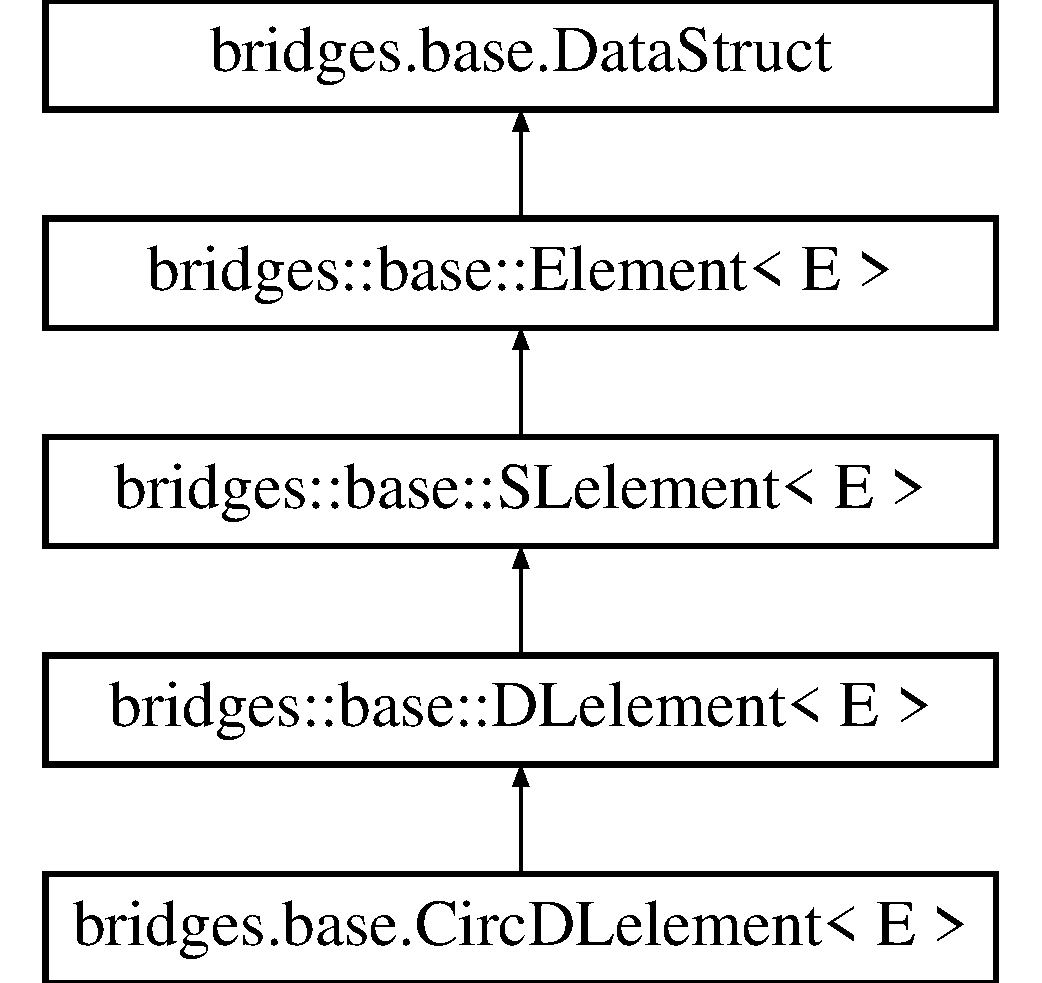
\includegraphics[height=5.000000cm]{classbridges_1_1base_1_1_circ_d_lelement}
\end{center}
\end{figure}


\subsection{Detailed Description}
This class can be used to instantiate Circular Doubly Linked List Elements. 

Structurally they are the same as doubly linked elements except that each node constructed with the next and the previous pointers points to itself.

User\textquotesingle{}s implementation of the circularly linked list needs to ensure that the last node\textquotesingle{}s next pointer points to the first node and the first node\textquotesingle{}s previous pointer points to the last node, as the visualization generation is dependent on this.

Elements have labels (string) that are displayed on the visualization. Elements take an generic object E as a user defined parameter, which can be any native type or object.

Elements contain a visualizer (\hyperlink{classbridges_1_1base_1_1_element_visualizer}{Element\+Visualizer}) object for setting visual attributes (color, shape, opacity, size), necessary for displaying them in a web browser.

Elements also have a \hyperlink{classbridges_1_1base_1_1_link_visualizer}{Link\+Visualizer} object that is used when they are linked to another element, appropriate for setting link attributes, between the element and its previous or next nodes.

\begin{DoxySeeAlso}{See also}
Example Tutorial at \href{http://bridgesuncc.github.io/tutorials/CircularDoublyLinkedList.html}{\tt http\+://bridgesuncc.\+github.\+io/tutorials/\+Circular\+Doubly\+Linked\+List.\+html}
\end{DoxySeeAlso}
\begin{DoxyAuthor}{Author}
Kalpathi Subramanian
\end{DoxyAuthor}
\begin{DoxyDate}{Date}
7/17/16, 1/16/17, 7/14/19
\end{DoxyDate}

\begin{DoxyParams}{Parameters}
{\em E} & the generic parameter object that contains application specific data, defined by the user when instantiating this object. \\
\hline
\end{DoxyParams}
\subsection*{Public Member Functions}
\begin{DoxyCompactItemize}
\item 
\hyperlink{classbridges_1_1base_1_1_circ_d_lelement_ad14ccb772d52c36802c118f2b3f15d59}{Circ\+D\+Lelement} ()
\item 
\hyperlink{classbridges_1_1base_1_1_circ_d_lelement_a84b2ebf47d2ca24077a800b240d8d157}{Circ\+D\+Lelement} (String label, E e)
\item 
\hyperlink{classbridges_1_1base_1_1_circ_d_lelement_a98a471fc3225ed80595e1ffdb377e336}{Circ\+D\+Lelement} (\hyperlink{classbridges_1_1base_1_1_circ_d_lelement}{Circ\+D\+Lelement}$<$ E $>$ \hyperlink{classbridges_1_1base_1_1_s_lelement_abf61c96a74ad319d561c6952ea388e0e}{next}, \hyperlink{classbridges_1_1base_1_1_circ_d_lelement}{Circ\+D\+Lelement}$<$ E $>$ \hyperlink{classbridges_1_1base_1_1_d_lelement_a6eba4876f820b75ac6bde01d7dea9da7}{prev})
\item 
\hyperlink{classbridges_1_1base_1_1_circ_d_lelement_a86e04c826251be9a1a92c4649844e5e7}{Circ\+D\+Lelement} (E e, \hyperlink{classbridges_1_1base_1_1_circ_d_lelement}{Circ\+D\+Lelement}$<$ E $>$ \hyperlink{classbridges_1_1base_1_1_s_lelement_abf61c96a74ad319d561c6952ea388e0e}{next}, \hyperlink{classbridges_1_1base_1_1_circ_d_lelement}{Circ\+D\+Lelement}$<$ E $>$ \hyperlink{classbridges_1_1base_1_1_d_lelement_a6eba4876f820b75ac6bde01d7dea9da7}{prev})
\item 
String \hyperlink{classbridges_1_1base_1_1_circ_d_lelement_ab4885ae7517f1dd04874270c1c3eaf44}{get\+Data\+Struct\+Type} ()
\item 
\hyperlink{classbridges_1_1base_1_1_circ_d_lelement}{Circ\+D\+Lelement}$<$ E $>$ \hyperlink{classbridges_1_1base_1_1_circ_d_lelement_a9ace56dde1f4c23e9a8798c045100ee6}{get\+Next} ()
\item 
\hyperlink{classbridges_1_1base_1_1_circ_d_lelement}{Circ\+D\+Lelement}$<$ E $>$ \hyperlink{classbridges_1_1base_1_1_circ_d_lelement_aa2b83017a571694460f77dd31b4188ed}{get\+Prev} ()
\end{DoxyCompactItemize}
\subsection*{Additional Inherited Members}


\subsection{Constructor \& Destructor Documentation}
\mbox{\Hypertarget{classbridges_1_1base_1_1_circ_d_lelement_ad14ccb772d52c36802c118f2b3f15d59}\label{classbridges_1_1base_1_1_circ_d_lelement_ad14ccb772d52c36802c118f2b3f15d59}} 
\index{bridges\+::base\+::\+Circ\+D\+Lelement@{bridges\+::base\+::\+Circ\+D\+Lelement}!Circ\+D\+Lelement@{Circ\+D\+Lelement}}
\index{Circ\+D\+Lelement@{Circ\+D\+Lelement}!bridges\+::base\+::\+Circ\+D\+Lelement@{bridges\+::base\+::\+Circ\+D\+Lelement}}
\subsubsection{\texorpdfstring{Circ\+D\+Lelement()}{CircDLelement()}\hspace{0.1cm}{\footnotesize\ttfamily [1/4]}}
{\footnotesize\ttfamily \hyperlink{classbridges_1_1base_1_1_circ_d_lelement}{bridges.\+base.\+Circ\+D\+Lelement}$<$ E $>$.\hyperlink{classbridges_1_1base_1_1_circ_d_lelement}{Circ\+D\+Lelement} (\begin{DoxyParamCaption}{ }\end{DoxyParamCaption})}

Constructs an empty \hyperlink{classbridges_1_1base_1_1_circ_d_lelement}{Circ\+D\+Lelement} with next and prev pointers set to itself \mbox{\Hypertarget{classbridges_1_1base_1_1_circ_d_lelement_a84b2ebf47d2ca24077a800b240d8d157}\label{classbridges_1_1base_1_1_circ_d_lelement_a84b2ebf47d2ca24077a800b240d8d157}} 
\index{bridges\+::base\+::\+Circ\+D\+Lelement@{bridges\+::base\+::\+Circ\+D\+Lelement}!Circ\+D\+Lelement@{Circ\+D\+Lelement}}
\index{Circ\+D\+Lelement@{Circ\+D\+Lelement}!bridges\+::base\+::\+Circ\+D\+Lelement@{bridges\+::base\+::\+Circ\+D\+Lelement}}
\subsubsection{\texorpdfstring{Circ\+D\+Lelement()}{CircDLelement()}\hspace{0.1cm}{\footnotesize\ttfamily [2/4]}}
{\footnotesize\ttfamily \hyperlink{classbridges_1_1base_1_1_circ_d_lelement}{bridges.\+base.\+Circ\+D\+Lelement}$<$ E $>$.\hyperlink{classbridges_1_1base_1_1_circ_d_lelement}{Circ\+D\+Lelement} (\begin{DoxyParamCaption}\item[{String}]{label,  }\item[{E}]{e }\end{DoxyParamCaption})}

Constructs a \hyperlink{classbridges_1_1base_1_1_circ_d_lelement}{Circ\+D\+Lelement} labeled \char`\"{}label\char`\"{}, holding an object \char`\"{}e\char`\"{}, with next and prev pointers set to itself


\begin{DoxyParams}{Parameters}
{\em label} & the label for this \hyperlink{classbridges_1_1base_1_1_circ_d_lelement}{Circ\+D\+Lelement} that shows up on the Bridges visualization \\
\hline
{\em e} & the genereic object that this \hyperlink{classbridges_1_1base_1_1_circ_d_lelement}{Circ\+D\+Lelement} is holding \\
\hline
\end{DoxyParams}
\mbox{\Hypertarget{classbridges_1_1base_1_1_circ_d_lelement_a98a471fc3225ed80595e1ffdb377e336}\label{classbridges_1_1base_1_1_circ_d_lelement_a98a471fc3225ed80595e1ffdb377e336}} 
\index{bridges\+::base\+::\+Circ\+D\+Lelement@{bridges\+::base\+::\+Circ\+D\+Lelement}!Circ\+D\+Lelement@{Circ\+D\+Lelement}}
\index{Circ\+D\+Lelement@{Circ\+D\+Lelement}!bridges\+::base\+::\+Circ\+D\+Lelement@{bridges\+::base\+::\+Circ\+D\+Lelement}}
\subsubsection{\texorpdfstring{Circ\+D\+Lelement()}{CircDLelement()}\hspace{0.1cm}{\footnotesize\ttfamily [3/4]}}
{\footnotesize\ttfamily \hyperlink{classbridges_1_1base_1_1_circ_d_lelement}{bridges.\+base.\+Circ\+D\+Lelement}$<$ E $>$.\hyperlink{classbridges_1_1base_1_1_circ_d_lelement}{Circ\+D\+Lelement} (\begin{DoxyParamCaption}\item[{\hyperlink{classbridges_1_1base_1_1_circ_d_lelement}{Circ\+D\+Lelement}$<$ E $>$}]{next,  }\item[{\hyperlink{classbridges_1_1base_1_1_circ_d_lelement}{Circ\+D\+Lelement}$<$ E $>$}]{prev }\end{DoxyParamCaption})}

Constructs an empty \hyperlink{classbridges_1_1base_1_1_d_lelement}{D\+Lelement} with the next pointer set to the \hyperlink{classbridges_1_1base_1_1_circ_d_lelement}{Circ\+D\+Lelement} \char`\"{}next\char`\"{} and the prev pointer set to \hyperlink{classbridges_1_1base_1_1_circ_d_lelement}{Circ\+D\+Lelement} \char`\"{}prev\char`\"{}.


\begin{DoxyParams}{Parameters}
{\em next} & the \hyperlink{classbridges_1_1base_1_1_d_lelement}{D\+Lelement} that should be assigned to the next pointer \\
\hline
{\em prev} & the \hyperlink{classbridges_1_1base_1_1_d_lelement}{D\+Lelement} that should be assigned to the prev pointer \\
\hline
\end{DoxyParams}
\mbox{\Hypertarget{classbridges_1_1base_1_1_circ_d_lelement_a86e04c826251be9a1a92c4649844e5e7}\label{classbridges_1_1base_1_1_circ_d_lelement_a86e04c826251be9a1a92c4649844e5e7}} 
\index{bridges\+::base\+::\+Circ\+D\+Lelement@{bridges\+::base\+::\+Circ\+D\+Lelement}!Circ\+D\+Lelement@{Circ\+D\+Lelement}}
\index{Circ\+D\+Lelement@{Circ\+D\+Lelement}!bridges\+::base\+::\+Circ\+D\+Lelement@{bridges\+::base\+::\+Circ\+D\+Lelement}}
\subsubsection{\texorpdfstring{Circ\+D\+Lelement()}{CircDLelement()}\hspace{0.1cm}{\footnotesize\ttfamily [4/4]}}
{\footnotesize\ttfamily \hyperlink{classbridges_1_1base_1_1_circ_d_lelement}{bridges.\+base.\+Circ\+D\+Lelement}$<$ E $>$.\hyperlink{classbridges_1_1base_1_1_circ_d_lelement}{Circ\+D\+Lelement} (\begin{DoxyParamCaption}\item[{E}]{e,  }\item[{\hyperlink{classbridges_1_1base_1_1_circ_d_lelement}{Circ\+D\+Lelement}$<$ E $>$}]{next,  }\item[{\hyperlink{classbridges_1_1base_1_1_circ_d_lelement}{Circ\+D\+Lelement}$<$ E $>$}]{prev }\end{DoxyParamCaption})}

Constructs a \hyperlink{classbridges_1_1base_1_1_d_lelement}{D\+Lelement} holding an object \char`\"{}e\char`\"{}, with the next pointer set to the \hyperlink{classbridges_1_1base_1_1_d_lelement}{D\+Lelement} \char`\"{}next\char`\"{} and the prev pointer set to \hyperlink{classbridges_1_1base_1_1_d_lelement}{D\+Lelement} \char`\"{}prev\char`\"{}.


\begin{DoxyParams}{Parameters}
{\em e} & the generic object that this \hyperlink{classbridges_1_1base_1_1_circ_d_lelement}{Circ\+D\+Lelement} is holding \\
\hline
{\em next} & the \hyperlink{classbridges_1_1base_1_1_circ_d_lelement}{Circ\+D\+Lelement} that should be assigned to the next pointer \\
\hline
{\em prev} & the \hyperlink{classbridges_1_1base_1_1_circ_d_lelement}{Circ\+D\+Lelement} that should be assigned to the prev pointer \\
\hline
\end{DoxyParams}


\subsection{Member Function Documentation}
\mbox{\Hypertarget{classbridges_1_1base_1_1_circ_d_lelement_ab4885ae7517f1dd04874270c1c3eaf44}\label{classbridges_1_1base_1_1_circ_d_lelement_ab4885ae7517f1dd04874270c1c3eaf44}} 
\index{bridges\+::base\+::\+Circ\+D\+Lelement@{bridges\+::base\+::\+Circ\+D\+Lelement}!get\+Data\+Struct\+Type@{get\+Data\+Struct\+Type}}
\index{get\+Data\+Struct\+Type@{get\+Data\+Struct\+Type}!bridges\+::base\+::\+Circ\+D\+Lelement@{bridges\+::base\+::\+Circ\+D\+Lelement}}
\subsubsection{\texorpdfstring{get\+Data\+Struct\+Type()}{getDataStructType()}}
{\footnotesize\ttfamily String \hyperlink{classbridges_1_1base_1_1_circ_d_lelement}{bridges.\+base.\+Circ\+D\+Lelement}$<$ E $>$.get\+Data\+Struct\+Type (\begin{DoxyParamCaption}{ }\end{DoxyParamCaption})}

This method gets the name of the data structure type

\begin{DoxyReturn}{Returns}
The date structure type as a string 
\end{DoxyReturn}
\mbox{\Hypertarget{classbridges_1_1base_1_1_circ_d_lelement_a9ace56dde1f4c23e9a8798c045100ee6}\label{classbridges_1_1base_1_1_circ_d_lelement_a9ace56dde1f4c23e9a8798c045100ee6}} 
\index{bridges\+::base\+::\+Circ\+D\+Lelement@{bridges\+::base\+::\+Circ\+D\+Lelement}!get\+Next@{get\+Next}}
\index{get\+Next@{get\+Next}!bridges\+::base\+::\+Circ\+D\+Lelement@{bridges\+::base\+::\+Circ\+D\+Lelement}}
\subsubsection{\texorpdfstring{get\+Next()}{getNext()}}
{\footnotesize\ttfamily \hyperlink{classbridges_1_1base_1_1_circ_d_lelement}{Circ\+D\+Lelement}$<$E$>$ \hyperlink{classbridges_1_1base_1_1_circ_d_lelement}{bridges.\+base.\+Circ\+D\+Lelement}$<$ E $>$.get\+Next (\begin{DoxyParamCaption}{ }\end{DoxyParamCaption})}

This method returns the pointer to the next \hyperlink{classbridges_1_1base_1_1_d_lelement}{D\+Lelement}

\begin{DoxyReturn}{Returns}
the \hyperlink{classbridges_1_1base_1_1_d_lelement}{D\+Lelement} assigned to the next pointer 
\end{DoxyReturn}
\mbox{\Hypertarget{classbridges_1_1base_1_1_circ_d_lelement_aa2b83017a571694460f77dd31b4188ed}\label{classbridges_1_1base_1_1_circ_d_lelement_aa2b83017a571694460f77dd31b4188ed}} 
\index{bridges\+::base\+::\+Circ\+D\+Lelement@{bridges\+::base\+::\+Circ\+D\+Lelement}!get\+Prev@{get\+Prev}}
\index{get\+Prev@{get\+Prev}!bridges\+::base\+::\+Circ\+D\+Lelement@{bridges\+::base\+::\+Circ\+D\+Lelement}}
\subsubsection{\texorpdfstring{get\+Prev()}{getPrev()}}
{\footnotesize\ttfamily \hyperlink{classbridges_1_1base_1_1_circ_d_lelement}{Circ\+D\+Lelement}$<$E$>$ \hyperlink{classbridges_1_1base_1_1_circ_d_lelement}{bridges.\+base.\+Circ\+D\+Lelement}$<$ E $>$.get\+Prev (\begin{DoxyParamCaption}{ }\end{DoxyParamCaption})}

This method returns the pointer to the previous \hyperlink{classbridges_1_1base_1_1_d_lelement}{D\+Lelement}

\begin{DoxyReturn}{Returns}
the \hyperlink{classbridges_1_1base_1_1_d_lelement}{D\+Lelement} assigned to the prev pointer 
\end{DoxyReturn}


The documentation for this class was generated from the following file\+:\begin{DoxyCompactItemize}
\item 
/home/erik/work/bridges/bridges-\/java/src/main/java/bridges/base/\hyperlink{_circ_d_lelement_8java}{Circ\+D\+Lelement.\+java}\end{DoxyCompactItemize}

\hypertarget{classbridges_1_1base_1_1_circ_s_lelement}{}\section{bridges.\+base.\+Circ\+S\+Lelement$<$ E $>$ Class Template Reference}
\label{classbridges_1_1base_1_1_circ_s_lelement}\index{bridges.\+base.\+Circ\+S\+Lelement$<$ E $>$@{bridges.\+base.\+Circ\+S\+Lelement$<$ E $>$}}


This class can be used to instantiate Singly Linked Circular List Elements.  


Inheritance diagram for bridges.\+base.\+Circ\+S\+Lelement$<$ E $>$\+:\begin{figure}[H]
\begin{center}
\leavevmode
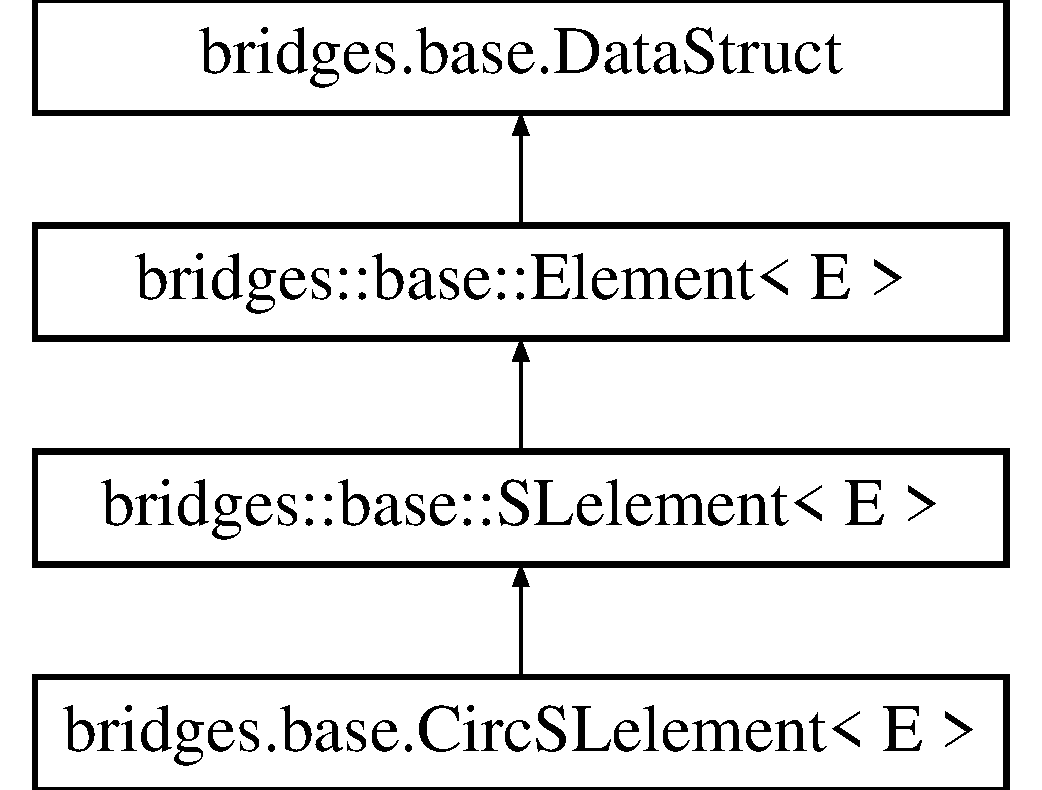
\includegraphics[height=4.000000cm]{classbridges_1_1base_1_1_circ_s_lelement}
\end{center}
\end{figure}
\subsection*{Public Member Functions}
\begin{DoxyCompactItemize}
\item 
\hyperlink{classbridges_1_1base_1_1_circ_s_lelement_a4a5a58cc7a0ec5170a828861c11df1b3}{Circ\+S\+Lelement} ()
\item 
\hyperlink{classbridges_1_1base_1_1_circ_s_lelement_a213d61713e51295d756669def911f080}{Circ\+S\+Lelement} (String label, E e)
\item 
\hyperlink{classbridges_1_1base_1_1_circ_s_lelement_ada65c593c8af7e6ed96fcdf12c26824f}{Circ\+S\+Lelement} (E e, \hyperlink{classbridges_1_1base_1_1_circ_s_lelement}{Circ\+S\+Lelement}$<$ E $>$ \hyperlink{classbridges_1_1base_1_1_s_lelement_abf61c96a74ad319d561c6952ea388e0e}{next})
\item 
\hyperlink{classbridges_1_1base_1_1_circ_s_lelement_ab9e5b98e8d917760b9651a52785358b9}{Circ\+S\+Lelement} (\hyperlink{classbridges_1_1base_1_1_circ_s_lelement}{Circ\+S\+Lelement}$<$ E $>$ \hyperlink{classbridges_1_1base_1_1_s_lelement_abf61c96a74ad319d561c6952ea388e0e}{next})
\item 
String \hyperlink{classbridges_1_1base_1_1_circ_s_lelement_ad56acddc52e8e0b6869a6f24f1e0a90e}{get\+Data\+Struct\+Type} ()
\item 
\hyperlink{classbridges_1_1base_1_1_circ_s_lelement}{Circ\+S\+Lelement}$<$ E $>$ \hyperlink{classbridges_1_1base_1_1_circ_s_lelement_ae18b07e3f1d37b5eca0cae22efc0d395}{get\+Next} ()
\item 
String \hyperlink{classbridges_1_1base_1_1_circ_s_lelement_af307188926766e73efb988f102ce9740}{to\+String} ()
\end{DoxyCompactItemize}
\subsection*{Additional Inherited Members}


\subsection{Detailed Description}
This class can be used to instantiate Singly Linked Circular List Elements. 

Structurally they are the same as singly linked elements except that each node constructed with the next point pointing to itself; User\textquotesingle{}s implementation of the circularly linked list needs to ensure that the last node points to first node of the list, as the visualization generation is dependent on this.

Elements have labels (string) that are displayed on the visualization. Elements take an generic object as a user defined parameter, E, which can be any native type or object.

Elements contains a visualizer (\hyperlink{classbridges_1_1base_1_1_element_visualizer}{Element\+Visualizer}) object for setting visual attributes (color, shape, opacity, size), necessary for displaying them in a web browser.

Elements also have a \hyperlink{classbridges_1_1base_1_1_link_visualizer}{Link\+Visualizer} object that is used when they are linked to another element, appropriate for setting link attributes, between an element and its next element.

\begin{DoxyAuthor}{Author}
Kalpathi Subramanian
\end{DoxyAuthor}
\begin{DoxyDate}{Date}
6/22/16, 1/7/17, 5/17/17
\end{DoxyDate}

\begin{DoxyParams}{Parameters}
{\em $<$\+E$>$} & the generic parameter that is defined by the application\\
\hline
\end{DoxyParams}
\begin{DoxySeeAlso}{See also}
Example Tutorial at ~\newline
 \href{http://bridgesuncc.github.io/Hello_World_Tutorials/CSLL.html}{\tt http\+://bridgesuncc.\+github.\+io/\+Hello\+\_\+\+World\+\_\+\+Tutorials/\+C\+S\+L\+L.\+html} 
\end{DoxySeeAlso}


\subsection{Constructor \& Destructor Documentation}
\hypertarget{classbridges_1_1base_1_1_circ_s_lelement_a4a5a58cc7a0ec5170a828861c11df1b3}{}\index{bridges\+::base\+::\+Circ\+S\+Lelement@{bridges\+::base\+::\+Circ\+S\+Lelement}!Circ\+S\+Lelement@{Circ\+S\+Lelement}}
\index{Circ\+S\+Lelement@{Circ\+S\+Lelement}!bridges\+::base\+::\+Circ\+S\+Lelement@{bridges\+::base\+::\+Circ\+S\+Lelement}}
\subsubsection[{Circ\+S\+Lelement()}]{\setlength{\rightskip}{0pt plus 5cm}{\bf bridges.\+base.\+Circ\+S\+Lelement}$<$ E $>$.{\bf Circ\+S\+Lelement} (
\begin{DoxyParamCaption}
{}
\end{DoxyParamCaption}
)}\label{classbridges_1_1base_1_1_circ_s_lelement_a4a5a58cc7a0ec5170a828861c11df1b3}
This constructor creates an \hyperlink{classbridges_1_1base_1_1_circ_s_lelement}{Circ\+S\+Lelement} object and sets its next pointer to itself \hypertarget{classbridges_1_1base_1_1_circ_s_lelement_a213d61713e51295d756669def911f080}{}\index{bridges\+::base\+::\+Circ\+S\+Lelement@{bridges\+::base\+::\+Circ\+S\+Lelement}!Circ\+S\+Lelement@{Circ\+S\+Lelement}}
\index{Circ\+S\+Lelement@{Circ\+S\+Lelement}!bridges\+::base\+::\+Circ\+S\+Lelement@{bridges\+::base\+::\+Circ\+S\+Lelement}}
\subsubsection[{Circ\+S\+Lelement(\+String label, E e)}]{\setlength{\rightskip}{0pt plus 5cm}{\bf bridges.\+base.\+Circ\+S\+Lelement}$<$ E $>$.{\bf Circ\+S\+Lelement} (
\begin{DoxyParamCaption}
\item[{String}]{label, }
\item[{E}]{e}
\end{DoxyParamCaption}
)}\label{classbridges_1_1base_1_1_circ_s_lelement_a213d61713e51295d756669def911f080}
This constructor creates an \hyperlink{classbridges_1_1base_1_1_circ_s_lelement}{Circ\+S\+Lelement} object of value \char`\"{}e\char`\"{} and label \char`\"{}label\char`\"{} and sets the next pointer to null


\begin{DoxyParams}{Parameters}
{\em label} & the label of \hyperlink{classbridges_1_1base_1_1_circ_s_lelement}{Circ\+S\+Lelement} that shows up on the Bridges visualization \\
\hline
{\em e} & the generic object that this \hyperlink{classbridges_1_1base_1_1_circ_s_lelement}{Circ\+S\+Lelement} will hold \\
\hline
\end{DoxyParams}
\hypertarget{classbridges_1_1base_1_1_circ_s_lelement_ada65c593c8af7e6ed96fcdf12c26824f}{}\index{bridges\+::base\+::\+Circ\+S\+Lelement@{bridges\+::base\+::\+Circ\+S\+Lelement}!Circ\+S\+Lelement@{Circ\+S\+Lelement}}
\index{Circ\+S\+Lelement@{Circ\+S\+Lelement}!bridges\+::base\+::\+Circ\+S\+Lelement@{bridges\+::base\+::\+Circ\+S\+Lelement}}
\subsubsection[{Circ\+S\+Lelement(\+E e, Circ\+S\+Lelement$<$ E $>$ next)}]{\setlength{\rightskip}{0pt plus 5cm}{\bf bridges.\+base.\+Circ\+S\+Lelement}$<$ E $>$.{\bf Circ\+S\+Lelement} (
\begin{DoxyParamCaption}
\item[{E}]{e, }
\item[{{\bf Circ\+S\+Lelement}$<$ E $>$}]{next}
\end{DoxyParamCaption}
)}\label{classbridges_1_1base_1_1_circ_s_lelement_ada65c593c8af7e6ed96fcdf12c26824f}
Creates a new element with value \char`\"{}e\char`\"{} and sets the next pointer to the \hyperlink{classbridges_1_1base_1_1_circ_s_lelement}{Circ\+S\+Lelement} referenced by the \char`\"{}next\char`\"{} argument


\begin{DoxyParams}{Parameters}
{\em e} & the generic object that this \hyperlink{classbridges_1_1base_1_1_circ_s_lelement}{Circ\+S\+Lelement} will hold \\
\hline
{\em next} & the \hyperlink{classbridges_1_1base_1_1_circ_s_lelement}{Circ\+S\+Lelement} that should be assigned to the next pointer \\
\hline
\end{DoxyParams}
\hypertarget{classbridges_1_1base_1_1_circ_s_lelement_ab9e5b98e8d917760b9651a52785358b9}{}\index{bridges\+::base\+::\+Circ\+S\+Lelement@{bridges\+::base\+::\+Circ\+S\+Lelement}!Circ\+S\+Lelement@{Circ\+S\+Lelement}}
\index{Circ\+S\+Lelement@{Circ\+S\+Lelement}!bridges\+::base\+::\+Circ\+S\+Lelement@{bridges\+::base\+::\+Circ\+S\+Lelement}}
\subsubsection[{Circ\+S\+Lelement(\+Circ\+S\+Lelement$<$ E $>$ next)}]{\setlength{\rightskip}{0pt plus 5cm}{\bf bridges.\+base.\+Circ\+S\+Lelement}$<$ E $>$.{\bf Circ\+S\+Lelement} (
\begin{DoxyParamCaption}
\item[{{\bf Circ\+S\+Lelement}$<$ E $>$}]{next}
\end{DoxyParamCaption}
)}\label{classbridges_1_1base_1_1_circ_s_lelement_ab9e5b98e8d917760b9651a52785358b9}
Creates a new element and sets the next pointer to the \hyperlink{classbridges_1_1base_1_1_circ_s_lelement}{Circ\+S\+Lelement} \char`\"{}next\char`\"{}


\begin{DoxyParams}{Parameters}
{\em next} & the \hyperlink{classbridges_1_1base_1_1_circ_s_lelement}{Circ\+S\+Lelement} that should be assigned to the next pointer \\
\hline
\end{DoxyParams}


\subsection{Member Function Documentation}
\hypertarget{classbridges_1_1base_1_1_circ_s_lelement_ad56acddc52e8e0b6869a6f24f1e0a90e}{}\index{bridges\+::base\+::\+Circ\+S\+Lelement@{bridges\+::base\+::\+Circ\+S\+Lelement}!get\+Data\+Struct\+Type@{get\+Data\+Struct\+Type}}
\index{get\+Data\+Struct\+Type@{get\+Data\+Struct\+Type}!bridges\+::base\+::\+Circ\+S\+Lelement@{bridges\+::base\+::\+Circ\+S\+Lelement}}
\subsubsection[{get\+Data\+Struct\+Type()}]{\setlength{\rightskip}{0pt plus 5cm}String {\bf bridges.\+base.\+Circ\+S\+Lelement}$<$ E $>$.get\+Data\+Struct\+Type (
\begin{DoxyParamCaption}
{}
\end{DoxyParamCaption}
)}\label{classbridges_1_1base_1_1_circ_s_lelement_ad56acddc52e8e0b6869a6f24f1e0a90e}
This method gets the data structure type

\begin{DoxyReturn}{Returns}
The date structure type as a string 
\end{DoxyReturn}
\hypertarget{classbridges_1_1base_1_1_circ_s_lelement_ae18b07e3f1d37b5eca0cae22efc0d395}{}\index{bridges\+::base\+::\+Circ\+S\+Lelement@{bridges\+::base\+::\+Circ\+S\+Lelement}!get\+Next@{get\+Next}}
\index{get\+Next@{get\+Next}!bridges\+::base\+::\+Circ\+S\+Lelement@{bridges\+::base\+::\+Circ\+S\+Lelement}}
\subsubsection[{get\+Next()}]{\setlength{\rightskip}{0pt plus 5cm}{\bf Circ\+S\+Lelement}$<$E$>$ {\bf bridges.\+base.\+Circ\+S\+Lelement}$<$ E $>$.get\+Next (
\begin{DoxyParamCaption}
{}
\end{DoxyParamCaption}
)}\label{classbridges_1_1base_1_1_circ_s_lelement_ae18b07e3f1d37b5eca0cae22efc0d395}
Retrieves the next \hyperlink{classbridges_1_1base_1_1_circ_s_lelement}{Circ\+S\+Lelement}

\begin{DoxyReturn}{Returns}
Circ\+S\+Lelement$<$\+E$>$ assigned to next 
\end{DoxyReturn}
\hypertarget{classbridges_1_1base_1_1_circ_s_lelement_af307188926766e73efb988f102ce9740}{}\index{bridges\+::base\+::\+Circ\+S\+Lelement@{bridges\+::base\+::\+Circ\+S\+Lelement}!to\+String@{to\+String}}
\index{to\+String@{to\+String}!bridges\+::base\+::\+Circ\+S\+Lelement@{bridges\+::base\+::\+Circ\+S\+Lelement}}
\subsubsection[{to\+String()}]{\setlength{\rightskip}{0pt plus 5cm}String {\bf bridges.\+base.\+Circ\+S\+Lelement}$<$ E $>$.to\+String (
\begin{DoxyParamCaption}
{}
\end{DoxyParamCaption}
)}\label{classbridges_1_1base_1_1_circ_s_lelement_af307188926766e73efb988f102ce9740}
(non-\/\+Javadoc)

\begin{DoxySeeAlso}{See also}
java.\+lang.\+Object\+::to\+String() 
\end{DoxySeeAlso}


The documentation for this class was generated from the following file\+:\begin{DoxyCompactItemize}
\item 
/\+Users/krs/gr/bridges/client/java/src/main/java/bridges/base/\hyperlink{_circ_s_lelement_8java}{Circ\+S\+Lelement.\+java}\end{DoxyCompactItemize}

\hypertarget{classbridges_1_1base_1_1_color}{}\section{bridges.\+base.\+Color Class Reference}
\label{classbridges_1_1base_1_1_color}\index{bridges.\+base.\+Color@{bridges.\+base.\+Color}}


This class is used to represent colors in B\+R\+I\+D\+G\+ES.  


\subsection*{Public Member Functions}
\begin{DoxyCompactItemize}
\item 
\mbox{\hyperlink{classbridges_1_1base_1_1_color_ab6d71ac2ee1430fb2db2fbe34e692de8}{Color}} ()
\item 
\mbox{\hyperlink{classbridges_1_1base_1_1_color_a15f56590ca3c9cc161c7bfa47060ad21}{Color}} (int r, int g, int b, float a)
\item 
\mbox{\hyperlink{classbridges_1_1base_1_1_color_a5fab564fa4eec8bece64f847ebd42948}{Color}} (int r, int g, int b)
\item 
\mbox{\hyperlink{classbridges_1_1base_1_1_color_a5cb17fdf8eddf44fc0763ceb7d4d833b}{Color}} (String color)
\item 
void \mbox{\hyperlink{classbridges_1_1base_1_1_color_a5559b1c7eb4c3901526b1012029b528f}{set\+Color}} (int r, int g, int b, float a)
\item 
void \mbox{\hyperlink{classbridges_1_1base_1_1_color_a1d78967703924b709e76def5b2b3ee9a}{set\+Red}} (int r)
\item 
int \mbox{\hyperlink{classbridges_1_1base_1_1_color_af1a30dc925b35d6bfe609f8838651025}{get\+Red}} ()
\item 
void \mbox{\hyperlink{classbridges_1_1base_1_1_color_a415a28133ade4e216c02ecdfc8a32a1d}{set\+Green}} (int g)
\item 
int \mbox{\hyperlink{classbridges_1_1base_1_1_color_a8f3fdd23cf785704faa2e3701e25978f}{get\+Green}} ()
\item 
void \mbox{\hyperlink{classbridges_1_1base_1_1_color_a0e04156b1573cf8002c4d9cb69825657}{set\+Blue}} (int b)
\item 
int \mbox{\hyperlink{classbridges_1_1base_1_1_color_ad4b82e1eb9ff59857d2868edd8d4ce65}{get\+Blue}} ()
\item 
void \mbox{\hyperlink{classbridges_1_1base_1_1_color_afab07ce64efa1fa5797795670b0effb6}{set\+Alpha}} (float a)
\item 
float \mbox{\hyperlink{classbridges_1_1base_1_1_color_a7c4247e31ecd8fcc61ef208d5deefe68}{get\+Alpha}} ()
\item 
String \mbox{\hyperlink{classbridges_1_1base_1_1_color_a2f9b0cb588e49b2ebf2f015d4d7507d0}{get\+Representation}} ()
\item 
String \mbox{\hyperlink{classbridges_1_1base_1_1_color_aced9bc89248b85686ba5385472974fe6}{get\+Hex\+Representation}} ()
\item 
byte \mbox{[}$\,$\mbox{]} \mbox{\hyperlink{classbridges_1_1base_1_1_color_a07215c888a6d17374a3d862ff30d5f93}{get\+Byte\+Representation}} ()
\item 
void \mbox{\hyperlink{classbridges_1_1base_1_1_color_a54dcd31227bde0f5d0a4f5d3b5a24ed2}{set\+Color}} (String col\+\_\+name)
\end{DoxyCompactItemize}


\subsection{Detailed Description}
This class is used to represent colors in B\+R\+I\+D\+G\+ES. 

We use an R\+G\+BA model to represent colors, with each component in the range 0-\/255. B\+R\+I\+D\+G\+ES also supports named colors for user convenience, but these are converted into \mbox{[}R\+G\+BA\mbox{]} prior to transmission to the server for visualization.

\begin{DoxyAuthor}{Author}
K.\+R. Subramanian, 
\end{DoxyAuthor}
\begin{DoxyDate}{Date}
7/14/16 
\end{DoxyDate}


\subsection{Constructor \& Destructor Documentation}
\mbox{\Hypertarget{classbridges_1_1base_1_1_color_ab6d71ac2ee1430fb2db2fbe34e692de8}\label{classbridges_1_1base_1_1_color_ab6d71ac2ee1430fb2db2fbe34e692de8}} 
\index{bridges\+::base\+::\+Color@{bridges\+::base\+::\+Color}!Color@{Color}}
\index{Color@{Color}!bridges\+::base\+::\+Color@{bridges\+::base\+::\+Color}}
\subsubsection{\texorpdfstring{Color()}{Color()}\hspace{0.1cm}{\footnotesize\ttfamily [1/4]}}
{\footnotesize\ttfamily bridges.\+base.\+Color.\+Color (\begin{DoxyParamCaption}{ }\end{DoxyParamCaption})}

Constructors \mbox{\Hypertarget{classbridges_1_1base_1_1_color_a15f56590ca3c9cc161c7bfa47060ad21}\label{classbridges_1_1base_1_1_color_a15f56590ca3c9cc161c7bfa47060ad21}} 
\index{bridges\+::base\+::\+Color@{bridges\+::base\+::\+Color}!Color@{Color}}
\index{Color@{Color}!bridges\+::base\+::\+Color@{bridges\+::base\+::\+Color}}
\subsubsection{\texorpdfstring{Color()}{Color()}\hspace{0.1cm}{\footnotesize\ttfamily [2/4]}}
{\footnotesize\ttfamily bridges.\+base.\+Color.\+Color (\begin{DoxyParamCaption}\item[{int}]{r,  }\item[{int}]{g,  }\item[{int}]{b,  }\item[{float}]{a }\end{DoxyParamCaption})}

Constructor, given r, g, b, a components


\begin{DoxyParams}{Parameters}
{\em r,g,b,a} & -\/ checked to be in the range 0-\/255 \\
\hline
\end{DoxyParams}
\mbox{\Hypertarget{classbridges_1_1base_1_1_color_a5fab564fa4eec8bece64f847ebd42948}\label{classbridges_1_1base_1_1_color_a5fab564fa4eec8bece64f847ebd42948}} 
\index{bridges\+::base\+::\+Color@{bridges\+::base\+::\+Color}!Color@{Color}}
\index{Color@{Color}!bridges\+::base\+::\+Color@{bridges\+::base\+::\+Color}}
\subsubsection{\texorpdfstring{Color()}{Color()}\hspace{0.1cm}{\footnotesize\ttfamily [3/4]}}
{\footnotesize\ttfamily bridges.\+base.\+Color.\+Color (\begin{DoxyParamCaption}\item[{int}]{r,  }\item[{int}]{g,  }\item[{int}]{b }\end{DoxyParamCaption})}

Constructor, given r, g, b components alpha (opacity) defaults to 255


\begin{DoxyParams}{Parameters}
{\em r,g,b,a} & -\/ checked to be in the range 0-\/255 \\
\hline
\end{DoxyParams}
\mbox{\Hypertarget{classbridges_1_1base_1_1_color_a5cb17fdf8eddf44fc0763ceb7d4d833b}\label{classbridges_1_1base_1_1_color_a5cb17fdf8eddf44fc0763ceb7d4d833b}} 
\index{bridges\+::base\+::\+Color@{bridges\+::base\+::\+Color}!Color@{Color}}
\index{Color@{Color}!bridges\+::base\+::\+Color@{bridges\+::base\+::\+Color}}
\subsubsection{\texorpdfstring{Color()}{Color()}\hspace{0.1cm}{\footnotesize\ttfamily [4/4]}}
{\footnotesize\ttfamily bridges.\+base.\+Color.\+Color (\begin{DoxyParamCaption}\item[{String}]{color }\end{DoxyParamCaption})}

Constructor, given color name


\begin{DoxyParams}{Parameters}
{\em color} & -\/ checked to be in the list of possible color names \\
\hline
\end{DoxyParams}


\subsection{Member Function Documentation}
\mbox{\Hypertarget{classbridges_1_1base_1_1_color_a7c4247e31ecd8fcc61ef208d5deefe68}\label{classbridges_1_1base_1_1_color_a7c4247e31ecd8fcc61ef208d5deefe68}} 
\index{bridges\+::base\+::\+Color@{bridges\+::base\+::\+Color}!get\+Alpha@{get\+Alpha}}
\index{get\+Alpha@{get\+Alpha}!bridges\+::base\+::\+Color@{bridges\+::base\+::\+Color}}
\subsubsection{\texorpdfstring{get\+Alpha()}{getAlpha()}}
{\footnotesize\ttfamily float bridges.\+base.\+Color.\+get\+Alpha (\begin{DoxyParamCaption}{ }\end{DoxyParamCaption})}

gets the alpha component

\begin{DoxyReturn}{Returns}
alpha -\/ returns the alpha(opacity) component of the color 
\end{DoxyReturn}
\mbox{\Hypertarget{classbridges_1_1base_1_1_color_ad4b82e1eb9ff59857d2868edd8d4ce65}\label{classbridges_1_1base_1_1_color_ad4b82e1eb9ff59857d2868edd8d4ce65}} 
\index{bridges\+::base\+::\+Color@{bridges\+::base\+::\+Color}!get\+Blue@{get\+Blue}}
\index{get\+Blue@{get\+Blue}!bridges\+::base\+::\+Color@{bridges\+::base\+::\+Color}}
\subsubsection{\texorpdfstring{get\+Blue()}{getBlue()}}
{\footnotesize\ttfamily int bridges.\+base.\+Color.\+get\+Blue (\begin{DoxyParamCaption}{ }\end{DoxyParamCaption})}

gets the blue component

\begin{DoxyReturn}{Returns}
blue -\/ returns the blue component of the color 
\end{DoxyReturn}
\mbox{\Hypertarget{classbridges_1_1base_1_1_color_a07215c888a6d17374a3d862ff30d5f93}\label{classbridges_1_1base_1_1_color_a07215c888a6d17374a3d862ff30d5f93}} 
\index{bridges\+::base\+::\+Color@{bridges\+::base\+::\+Color}!get\+Byte\+Representation@{get\+Byte\+Representation}}
\index{get\+Byte\+Representation@{get\+Byte\+Representation}!bridges\+::base\+::\+Color@{bridges\+::base\+::\+Color}}
\subsubsection{\texorpdfstring{get\+Byte\+Representation()}{getByteRepresentation()}}
{\footnotesize\ttfamily byte \mbox{[}$\,$\mbox{]} bridges.\+base.\+Color.\+get\+Byte\+Representation (\begin{DoxyParamCaption}{ }\end{DoxyParamCaption})}

gets a Byte array representation of a \mbox{\hyperlink{classbridges_1_1base_1_1_color}{Color}}

\begin{DoxyReturn}{Returns}
-\/ returns the R\+G\+BA color as a byte array 
\end{DoxyReturn}
\mbox{\Hypertarget{classbridges_1_1base_1_1_color_a8f3fdd23cf785704faa2e3701e25978f}\label{classbridges_1_1base_1_1_color_a8f3fdd23cf785704faa2e3701e25978f}} 
\index{bridges\+::base\+::\+Color@{bridges\+::base\+::\+Color}!get\+Green@{get\+Green}}
\index{get\+Green@{get\+Green}!bridges\+::base\+::\+Color@{bridges\+::base\+::\+Color}}
\subsubsection{\texorpdfstring{get\+Green()}{getGreen()}}
{\footnotesize\ttfamily int bridges.\+base.\+Color.\+get\+Green (\begin{DoxyParamCaption}{ }\end{DoxyParamCaption})}

gets the green component

\begin{DoxyReturn}{Returns}
green -\/ returns the green component of the color 
\end{DoxyReturn}
\mbox{\Hypertarget{classbridges_1_1base_1_1_color_aced9bc89248b85686ba5385472974fe6}\label{classbridges_1_1base_1_1_color_aced9bc89248b85686ba5385472974fe6}} 
\index{bridges\+::base\+::\+Color@{bridges\+::base\+::\+Color}!get\+Hex\+Representation@{get\+Hex\+Representation}}
\index{get\+Hex\+Representation@{get\+Hex\+Representation}!bridges\+::base\+::\+Color@{bridges\+::base\+::\+Color}}
\subsubsection{\texorpdfstring{get\+Hex\+Representation()}{getHexRepresentation()}}
{\footnotesize\ttfamily String bridges.\+base.\+Color.\+get\+Hex\+Representation (\begin{DoxyParamCaption}{ }\end{DoxyParamCaption})}

gets the R\+GB \mbox{\hyperlink{classbridges_1_1base_1_1_color}{Color}} representation as a Hex String

\begin{DoxyReturn}{Returns}
-\/ returns the R\+GB color as hexadecimal String 
\end{DoxyReturn}
\mbox{\Hypertarget{classbridges_1_1base_1_1_color_af1a30dc925b35d6bfe609f8838651025}\label{classbridges_1_1base_1_1_color_af1a30dc925b35d6bfe609f8838651025}} 
\index{bridges\+::base\+::\+Color@{bridges\+::base\+::\+Color}!get\+Red@{get\+Red}}
\index{get\+Red@{get\+Red}!bridges\+::base\+::\+Color@{bridges\+::base\+::\+Color}}
\subsubsection{\texorpdfstring{get\+Red()}{getRed()}}
{\footnotesize\ttfamily int bridges.\+base.\+Color.\+get\+Red (\begin{DoxyParamCaption}{ }\end{DoxyParamCaption})}

gets the red component

\begin{DoxyReturn}{Returns}
red -\/ returns the red component of the color 
\end{DoxyReturn}
\mbox{\Hypertarget{classbridges_1_1base_1_1_color_a2f9b0cb588e49b2ebf2f015d4d7507d0}\label{classbridges_1_1base_1_1_color_a2f9b0cb588e49b2ebf2f015d4d7507d0}} 
\index{bridges\+::base\+::\+Color@{bridges\+::base\+::\+Color}!get\+Representation@{get\+Representation}}
\index{get\+Representation@{get\+Representation}!bridges\+::base\+::\+Color@{bridges\+::base\+::\+Color}}
\subsubsection{\texorpdfstring{get\+Representation()}{getRepresentation()}}
{\footnotesize\ttfamily String bridges.\+base.\+Color.\+get\+Representation (\begin{DoxyParamCaption}{ }\end{DoxyParamCaption})}

gets the \mbox{\hyperlink{classbridges_1_1base_1_1_color}{Color}} representation as a String

\begin{DoxyReturn}{Returns}
-\/ returns the color as a String with an R\+G\+BA array format 
\end{DoxyReturn}
\mbox{\Hypertarget{classbridges_1_1base_1_1_color_afab07ce64efa1fa5797795670b0effb6}\label{classbridges_1_1base_1_1_color_afab07ce64efa1fa5797795670b0effb6}} 
\index{bridges\+::base\+::\+Color@{bridges\+::base\+::\+Color}!set\+Alpha@{set\+Alpha}}
\index{set\+Alpha@{set\+Alpha}!bridges\+::base\+::\+Color@{bridges\+::base\+::\+Color}}
\subsubsection{\texorpdfstring{set\+Alpha()}{setAlpha()}}
{\footnotesize\ttfamily void bridges.\+base.\+Color.\+set\+Alpha (\begin{DoxyParamCaption}\item[{float}]{a }\end{DoxyParamCaption})}

sets the alpha(opacity) component


\begin{DoxyParams}{Parameters}
{\em a} & -\/ checked to be in the range 0-\/255 \\
\hline
\end{DoxyParams}
\mbox{\Hypertarget{classbridges_1_1base_1_1_color_a0e04156b1573cf8002c4d9cb69825657}\label{classbridges_1_1base_1_1_color_a0e04156b1573cf8002c4d9cb69825657}} 
\index{bridges\+::base\+::\+Color@{bridges\+::base\+::\+Color}!set\+Blue@{set\+Blue}}
\index{set\+Blue@{set\+Blue}!bridges\+::base\+::\+Color@{bridges\+::base\+::\+Color}}
\subsubsection{\texorpdfstring{set\+Blue()}{setBlue()}}
{\footnotesize\ttfamily void bridges.\+base.\+Color.\+set\+Blue (\begin{DoxyParamCaption}\item[{int}]{b }\end{DoxyParamCaption})}

sets the blue component


\begin{DoxyParams}{Parameters}
{\em b} & -\/ checked to be in the range 0-\/255 \\
\hline
\end{DoxyParams}
\mbox{\Hypertarget{classbridges_1_1base_1_1_color_a5559b1c7eb4c3901526b1012029b528f}\label{classbridges_1_1base_1_1_color_a5559b1c7eb4c3901526b1012029b528f}} 
\index{bridges\+::base\+::\+Color@{bridges\+::base\+::\+Color}!set\+Color@{set\+Color}}
\index{set\+Color@{set\+Color}!bridges\+::base\+::\+Color@{bridges\+::base\+::\+Color}}
\subsubsection{\texorpdfstring{set\+Color()}{setColor()}\hspace{0.1cm}{\footnotesize\ttfamily [1/2]}}
{\footnotesize\ttfamily void bridges.\+base.\+Color.\+set\+Color (\begin{DoxyParamCaption}\item[{int}]{r,  }\item[{int}]{g,  }\item[{int}]{b,  }\item[{float}]{a }\end{DoxyParamCaption})}

sets color to the given r, g, b, a components


\begin{DoxyParams}{Parameters}
{\em r,g,b,a} & -\/ checked to be in the range 0-\/255 \\
\hline
\end{DoxyParams}
\mbox{\Hypertarget{classbridges_1_1base_1_1_color_a54dcd31227bde0f5d0a4f5d3b5a24ed2}\label{classbridges_1_1base_1_1_color_a54dcd31227bde0f5d0a4f5d3b5a24ed2}} 
\index{bridges\+::base\+::\+Color@{bridges\+::base\+::\+Color}!set\+Color@{set\+Color}}
\index{set\+Color@{set\+Color}!bridges\+::base\+::\+Color@{bridges\+::base\+::\+Color}}
\subsubsection{\texorpdfstring{set\+Color()}{setColor()}\hspace{0.1cm}{\footnotesize\ttfamily [2/2]}}
{\footnotesize\ttfamily void bridges.\+base.\+Color.\+set\+Color (\begin{DoxyParamCaption}\item[{String}]{col\+\_\+name }\end{DoxyParamCaption})}

sets the color to the R\+G\+BA components given the color name


\begin{DoxyParams}{Parameters}
{\em col\+\_\+name} & color name \\
\hline
\end{DoxyParams}
\mbox{\Hypertarget{classbridges_1_1base_1_1_color_a415a28133ade4e216c02ecdfc8a32a1d}\label{classbridges_1_1base_1_1_color_a415a28133ade4e216c02ecdfc8a32a1d}} 
\index{bridges\+::base\+::\+Color@{bridges\+::base\+::\+Color}!set\+Green@{set\+Green}}
\index{set\+Green@{set\+Green}!bridges\+::base\+::\+Color@{bridges\+::base\+::\+Color}}
\subsubsection{\texorpdfstring{set\+Green()}{setGreen()}}
{\footnotesize\ttfamily void bridges.\+base.\+Color.\+set\+Green (\begin{DoxyParamCaption}\item[{int}]{g }\end{DoxyParamCaption})}

sets the green component


\begin{DoxyParams}{Parameters}
{\em g} & -\/ checked to be in the range 0-\/255 \\
\hline
\end{DoxyParams}
\mbox{\Hypertarget{classbridges_1_1base_1_1_color_a1d78967703924b709e76def5b2b3ee9a}\label{classbridges_1_1base_1_1_color_a1d78967703924b709e76def5b2b3ee9a}} 
\index{bridges\+::base\+::\+Color@{bridges\+::base\+::\+Color}!set\+Red@{set\+Red}}
\index{set\+Red@{set\+Red}!bridges\+::base\+::\+Color@{bridges\+::base\+::\+Color}}
\subsubsection{\texorpdfstring{set\+Red()}{setRed()}}
{\footnotesize\ttfamily void bridges.\+base.\+Color.\+set\+Red (\begin{DoxyParamCaption}\item[{int}]{r }\end{DoxyParamCaption})}

sets the red component


\begin{DoxyParams}{Parameters}
{\em r} & -\/ checked to be in the range 0-\/255 \\
\hline
\end{DoxyParams}


The documentation for this class was generated from the following file\+:\begin{DoxyCompactItemize}
\item 
/\+Users/kalpathi/gr/bridges/client/java/bridges-\/17/src/main/java/edu/uncc/cs/bridges\+\_\+v21/base/\mbox{\hyperlink{_color_8java}{Color.\+java}}\end{DoxyCompactItemize}

\hypertarget{classbridges_1_1base_1_1_color_grid}{}\doxysection{bridges.\+base.\+Color\+Grid Class Reference}
\label{classbridges_1_1base_1_1_color_grid}\index{bridges.base.ColorGrid@{bridges.base.ColorGrid}}
Inheritance diagram for bridges.\+base.\+Color\+Grid\+:\begin{figure}[H]
\begin{center}
\leavevmode
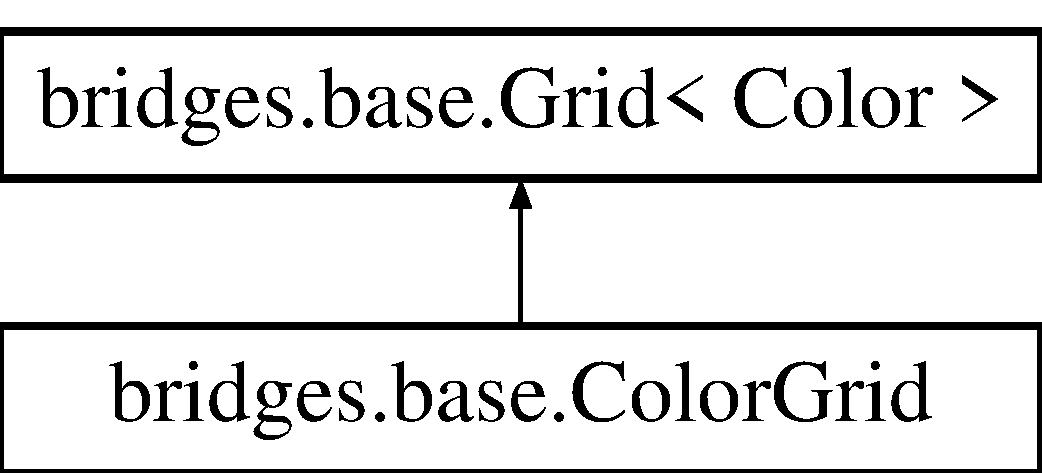
\includegraphics[height=2.000000cm]{classbridges_1_1base_1_1_color_grid}
\end{center}
\end{figure}


\doxysubsection{Detailed Description}
This is a class in B\+R\+I\+D\+G\+ES for representing an image. 

A \mbox{\hyperlink{classbridges_1_1base_1_1_color_grid}{Color\+Grid}} is essentially an image. One can construct an image of a particular size using the \mbox{\hyperlink{classbridges_1_1base_1_1_color_grid_af434a5a3dcbaf86e51ac6f9e1c1d7e5f}{Color\+Grid()}} constructor to be either blank or filled with a particular \mbox{\hyperlink{classbridges_1_1base_1_1_color}{Color}} depending on which constructor is called.

One can change the color of a pixel with \mbox{\hyperlink{classbridges_1_1base_1_1_grid_ab79ceb737423bb28ea2348e61a625a17}{set()}}. For instance, like that\+: 
\begin{DoxyCode}{0}
\DoxyCodeLine{\mbox{\hyperlink{classbridges_1_1base_1_1_color_grid_af434a5a3dcbaf86e51ac6f9e1c1d7e5f}{ColorGrid}} \mbox{\hyperlink{classbridges_1_1base_1_1_grid_ad1f3f6968d58188425bd992c05c655a6}{grid}} = \textcolor{keyword}{new} \mbox{\hyperlink{classbridges_1_1base_1_1_color_grid_af434a5a3dcbaf86e51ac6f9e1c1d7e5f}{ColorGrid}}(rows, columns);}
\DoxyCodeLine{\mbox{\hyperlink{classbridges_1_1base_1_1_grid_ad1f3f6968d58188425bd992c05c655a6}{grid}}.set (2, 3, \textcolor{keyword}{new} Color(\textcolor{stringliteral}{"lightsalmon"});}
\end{DoxyCode}


You can get a \mbox{\hyperlink{classbridges_1_1base_1_1_color_grid}{Color\+Grid}} from an existing Bridges \mbox{\hyperlink{classbridges_1_1base_1_1_color_grid}{Color\+Grid}} assignment using \mbox{\hyperlink{classbridges_1_1connect_1_1_data_source_a9556950d89b39ce61bead0879d1e2192}{bridges.\+connect.\+Data\+Source.\+get\+Color\+Grid\+From\+Assignment()}}

\begin{DoxySeeAlso}{See also}
There is a tutorial about \mbox{\hyperlink{classbridges_1_1base_1_1_color_grid}{Color\+Grid}} \+: \href{http://bridgesuncc.github.io/tutorials/Grid.html}{\texttt{ http\+://bridgesuncc.\+github.\+io/tutorials/\+Grid.\+html}}
\end{DoxySeeAlso}
\begin{DoxyAuthor}{Author}
David Burlinson, Erik Saule 
\end{DoxyAuthor}
\doxysubsection*{Public Member Functions}
\begin{DoxyCompactItemize}
\item 
String \mbox{\hyperlink{classbridges_1_1base_1_1_color_grid_a53a1f3f105f8545796f98e5fac559b5b}{get\+Data\+Struct\+Type}} ()
\item 
\mbox{\hyperlink{classbridges_1_1base_1_1_color_grid_af434a5a3dcbaf86e51ac6f9e1c1d7e5f}{Color\+Grid}} ()
\item 
\mbox{\hyperlink{classbridges_1_1base_1_1_color_grid_aafb4157a4c8129f30c1f989fcdfda544}{Color\+Grid}} (int rows, int cols)
\item 
\mbox{\hyperlink{classbridges_1_1base_1_1_color_grid_aef40242c93b66ab851e6afa64cada0b5}{Color\+Grid}} (int rows, int cols, \mbox{\hyperlink{classbridges_1_1base_1_1_color}{Color}} color)
\item 
int \mbox{\hyperlink{classbridges_1_1base_1_1_color_grid_a8793791e35f03b3e5a2e5ef3606ac124}{get\+Height}} ()
\item 
int \mbox{\hyperlink{classbridges_1_1base_1_1_color_grid_af872226de86ac8e8f2553fdc5bddc375}{get\+Width}} ()
\item 
String \mbox{\hyperlink{classbridges_1_1base_1_1_color_grid_a81ca0995d17b6cb31122b718dfa57286}{get\+Data\+Structure\+Representation}} ()
\end{DoxyCompactItemize}
\doxysubsection*{Additional Inherited Members}


\doxysubsection{Constructor \& Destructor Documentation}
\mbox{\Hypertarget{classbridges_1_1base_1_1_color_grid_af434a5a3dcbaf86e51ac6f9e1c1d7e5f}\label{classbridges_1_1base_1_1_color_grid_af434a5a3dcbaf86e51ac6f9e1c1d7e5f}} 
\index{bridges.base.ColorGrid@{bridges.base.ColorGrid}!ColorGrid@{ColorGrid}}
\index{ColorGrid@{ColorGrid}!bridges.base.ColorGrid@{bridges.base.ColorGrid}}
\doxysubsubsection{\texorpdfstring{ColorGrid()}{ColorGrid()}\hspace{0.1cm}{\footnotesize\ttfamily [1/3]}}
{\footnotesize\ttfamily bridges.\+base.\+Color\+Grid.\+Color\+Grid (\begin{DoxyParamCaption}{ }\end{DoxyParamCaption})}

Construct a color grid with defaulty sizes\+: \mbox{\Hypertarget{classbridges_1_1base_1_1_color_grid_aafb4157a4c8129f30c1f989fcdfda544}\label{classbridges_1_1base_1_1_color_grid_aafb4157a4c8129f30c1f989fcdfda544}} 
\index{bridges.base.ColorGrid@{bridges.base.ColorGrid}!ColorGrid@{ColorGrid}}
\index{ColorGrid@{ColorGrid}!bridges.base.ColorGrid@{bridges.base.ColorGrid}}
\doxysubsubsection{\texorpdfstring{ColorGrid()}{ColorGrid()}\hspace{0.1cm}{\footnotesize\ttfamily [2/3]}}
{\footnotesize\ttfamily bridges.\+base.\+Color\+Grid.\+Color\+Grid (\begin{DoxyParamCaption}\item[{int}]{rows,  }\item[{int}]{cols }\end{DoxyParamCaption})}

\mbox{\hyperlink{classbridges_1_1base_1_1_grid}{Grid}} constructor with size arguments


\begin{DoxyParams}{Parameters}
{\em rows} & -\/ int representing the number of rows of the grid \\
\hline
{\em cols} & -\/ int representing the number of columns of the grid \\
\hline
\end{DoxyParams}
\mbox{\Hypertarget{classbridges_1_1base_1_1_color_grid_aef40242c93b66ab851e6afa64cada0b5}\label{classbridges_1_1base_1_1_color_grid_aef40242c93b66ab851e6afa64cada0b5}} 
\index{bridges.base.ColorGrid@{bridges.base.ColorGrid}!ColorGrid@{ColorGrid}}
\index{ColorGrid@{ColorGrid}!bridges.base.ColorGrid@{bridges.base.ColorGrid}}
\doxysubsubsection{\texorpdfstring{ColorGrid()}{ColorGrid()}\hspace{0.1cm}{\footnotesize\ttfamily [3/3]}}
{\footnotesize\ttfamily bridges.\+base.\+Color\+Grid.\+Color\+Grid (\begin{DoxyParamCaption}\item[{int}]{rows,  }\item[{int}]{cols,  }\item[{\mbox{\hyperlink{classbridges_1_1base_1_1_color}{Color}}}]{color }\end{DoxyParamCaption})}

\mbox{\hyperlink{classbridges_1_1base_1_1_grid}{Grid}} constructor with size and color string argument


\begin{DoxyParams}{Parameters}
{\em rows} & -\/ int representing the number of rows of the grid \\
\hline
{\em cols} & -\/ int representing the number of columns of the grid \\
\hline
{\em color} & -\/ \mbox{\hyperlink{classbridges_1_1base_1_1_color}{Color}} object \\
\hline
\end{DoxyParams}


\doxysubsection{Member Function Documentation}
\mbox{\Hypertarget{classbridges_1_1base_1_1_color_grid_a53a1f3f105f8545796f98e5fac559b5b}\label{classbridges_1_1base_1_1_color_grid_a53a1f3f105f8545796f98e5fac559b5b}} 
\index{bridges.base.ColorGrid@{bridges.base.ColorGrid}!getDataStructType@{getDataStructType}}
\index{getDataStructType@{getDataStructType}!bridges.base.ColorGrid@{bridges.base.ColorGrid}}
\doxysubsubsection{\texorpdfstring{getDataStructType()}{getDataStructType()}}
{\footnotesize\ttfamily String bridges.\+base.\+Color\+Grid.\+get\+Data\+Struct\+Type (\begin{DoxyParamCaption}{ }\end{DoxyParamCaption})}

Get the data type name \begin{DoxyReturn}{Returns}
the data type 
\end{DoxyReturn}
\mbox{\Hypertarget{classbridges_1_1base_1_1_color_grid_a81ca0995d17b6cb31122b718dfa57286}\label{classbridges_1_1base_1_1_color_grid_a81ca0995d17b6cb31122b718dfa57286}} 
\index{bridges.base.ColorGrid@{bridges.base.ColorGrid}!getDataStructureRepresentation@{getDataStructureRepresentation}}
\index{getDataStructureRepresentation@{getDataStructureRepresentation}!bridges.base.ColorGrid@{bridges.base.ColorGrid}}
\doxysubsubsection{\texorpdfstring{getDataStructureRepresentation()}{getDataStructureRepresentation()}}
{\footnotesize\ttfamily String bridges.\+base.\+Color\+Grid.\+get\+Data\+Structure\+Representation (\begin{DoxyParamCaption}{ }\end{DoxyParamCaption})}

Get the J\+S\+ON representation of the color grid

\begin{DoxyReturn}{Returns}
the J\+S\+ON representation (string) of the color grid 
\end{DoxyReturn}
\mbox{\Hypertarget{classbridges_1_1base_1_1_color_grid_a8793791e35f03b3e5a2e5ef3606ac124}\label{classbridges_1_1base_1_1_color_grid_a8793791e35f03b3e5a2e5ef3606ac124}} 
\index{bridges.base.ColorGrid@{bridges.base.ColorGrid}!getHeight@{getHeight}}
\index{getHeight@{getHeight}!bridges.base.ColorGrid@{bridges.base.ColorGrid}}
\doxysubsubsection{\texorpdfstring{getHeight()}{getHeight()}}
{\footnotesize\ttfamily int bridges.\+base.\+Color\+Grid.\+get\+Height (\begin{DoxyParamCaption}{ }\end{DoxyParamCaption})}

Get the height of the color grid

\begin{DoxyReturn}{Returns}
the height (number of rows) of the grid 
\end{DoxyReturn}
\mbox{\Hypertarget{classbridges_1_1base_1_1_color_grid_af872226de86ac8e8f2553fdc5bddc375}\label{classbridges_1_1base_1_1_color_grid_af872226de86ac8e8f2553fdc5bddc375}} 
\index{bridges.base.ColorGrid@{bridges.base.ColorGrid}!getWidth@{getWidth}}
\index{getWidth@{getWidth}!bridges.base.ColorGrid@{bridges.base.ColorGrid}}
\doxysubsubsection{\texorpdfstring{getWidth()}{getWidth()}}
{\footnotesize\ttfamily int bridges.\+base.\+Color\+Grid.\+get\+Width (\begin{DoxyParamCaption}{ }\end{DoxyParamCaption})}

Get the width of the color grid

\begin{DoxyReturn}{Returns}
the width (number of columns) of the grid 
\end{DoxyReturn}


The documentation for this class was generated from the following file\+:\begin{DoxyCompactItemize}
\item 
/\+Users/kalpathi/gr/bridges/client/java/src/main/java/bridges/base/\mbox{\hyperlink{_color_grid_8java}{Color\+Grid.\+java}}\end{DoxyCompactItemize}

\hypertarget{classbridges_1_1connect_1_1_connector}{}\section{bridges.\+connect.\+Connector Class Reference}
\label{classbridges_1_1connect_1_1_connector}\index{bridges.\+connect.\+Connector@{bridges.\+connect.\+Connector}}
\subsection*{Public Member Functions}
\begin{DoxyCompactItemize}
\item 
void \hyperlink{classbridges_1_1connect_1_1_connector_acab24a8c4ffd3349ec67536552fb30b3}{set\+Server} (String server)  throws Illegal\+Argument\+Exception 
\item 
String \hyperlink{classbridges_1_1connect_1_1_connector_a0b9809180aac96a83e31e224ab5ed6ec}{get\+Server\+U\+R\+L} ()
\item 
void \hyperlink{classbridges_1_1connect_1_1_connector_a71f449c91e529f79730df27e01fdf674}{set\+Server\+U\+R\+L} (String server\+\_\+url)
\item 
String \hyperlink{classbridges_1_1connect_1_1_connector_a2318cd93d18ef58285598f6f9cdf727b}{latlong\+Formatter} (String text)
\item 
String \hyperlink{classbridges_1_1connect_1_1_connector_ac0dca0bd99b6abbbd8a77874a95e6d49}{trimm\+Last} (String text)
\item 
J\+S\+O\+N\+Object \hyperlink{classbridges_1_1connect_1_1_connector_aac3fb75dd7975c4439cfd1bf6cefe0a6}{as\+J\+S\+O\+N\+Object} (String text)  throws I\+O\+Exception 
\item 
J\+S\+O\+N\+Array \hyperlink{classbridges_1_1connect_1_1_connector_aa5bd647713545fa24c6d730eacb6bc54}{as\+J\+S\+O\+N\+Array} (String text)  throws I\+O\+Exception 
\item 
Object \hyperlink{classbridges_1_1connect_1_1_connector_ab7d1d242fbf9acade316650e54a3d020}{safe\+J\+S\+O\+N\+Traverse} (String sequence, Object original, Class$<$?$>$ target)  throws I\+O\+Exception 
\item 
String \hyperlink{classbridges_1_1connect_1_1_connector_aabcfde23d155c8c42edb8a1407320bc5}{execute\+H\+T\+T\+P\+Request} (Request request)  throws Client\+Protocol\+Exception, I\+O\+Exception, Rate\+Limit\+Exception 
\item 
String \hyperlink{classbridges_1_1connect_1_1_connector_aec8d54bf707c50d6f8173a0c1640fcd5}{get} (String url)  throws Rate\+Limit\+Exception, I\+O\+Exception 
\item 
String \hyperlink{classbridges_1_1connect_1_1_connector_a1781405c9b38c338bce042bf7ff23eaf}{get\+U\+S\+G\+S} (String url)  throws Rate\+Limit\+Exception, I\+O\+Exception 
\item 
String \hyperlink{classbridges_1_1connect_1_1_connector_a88e465aed707d59b96958dcc946ff6b4}{post} (String url, Map$<$ String, String $>$ arguments)  throws I\+O\+Exception, Rate\+Limit\+Exception 
\item 
String \hyperlink{classbridges_1_1connect_1_1_connector_a4b8978743a8c230b86500f5a00cb2697}{post} (String url, String data)  throws I\+O\+Exception, 		\+Rate\+Limit\+Exception 
\item 
String \hyperlink{classbridges_1_1connect_1_1_connector_a507ee5a9d8c812ffd4629cbd22f27373}{prepare} (String url)
\item 
String \hyperlink{classbridges_1_1connect_1_1_connector_aa0201e2569358ff906d3c14d654711e5}{prepare\+U\+S\+G\+S} (String url)
\end{DoxyCompactItemize}
\subsection*{Protected Member Functions}
\begin{DoxyCompactItemize}
\item 
\hyperlink{classbridges_1_1connect_1_1_connector_a167800699b2d191bd625d9c8c8cd9e6f}{Connector} ()
\end{DoxyCompactItemize}


\subsection{Constructor \& Destructor Documentation}
\hypertarget{classbridges_1_1connect_1_1_connector_a167800699b2d191bd625d9c8c8cd9e6f}{}\index{bridges\+::connect\+::\+Connector@{bridges\+::connect\+::\+Connector}!Connector@{Connector}}
\index{Connector@{Connector}!bridges\+::connect\+::\+Connector@{bridges\+::connect\+::\+Connector}}
\subsubsection[{Connector()}]{\setlength{\rightskip}{0pt plus 5cm}bridges.\+connect.\+Connector.\+Connector (
\begin{DoxyParamCaption}
{}
\end{DoxyParamCaption}
)\hspace{0.3cm}{\ttfamily [protected]}}\label{classbridges_1_1connect_1_1_connector_a167800699b2d191bd625d9c8c8cd9e6f}


\subsection{Member Function Documentation}
\hypertarget{classbridges_1_1connect_1_1_connector_aa5bd647713545fa24c6d730eacb6bc54}{}\index{bridges\+::connect\+::\+Connector@{bridges\+::connect\+::\+Connector}!as\+J\+S\+O\+N\+Array@{as\+J\+S\+O\+N\+Array}}
\index{as\+J\+S\+O\+N\+Array@{as\+J\+S\+O\+N\+Array}!bridges\+::connect\+::\+Connector@{bridges\+::connect\+::\+Connector}}
\subsubsection[{as\+J\+S\+O\+N\+Array(\+String text)}]{\setlength{\rightskip}{0pt plus 5cm}J\+S\+O\+N\+Array bridges.\+connect.\+Connector.\+as\+J\+S\+O\+N\+Array (
\begin{DoxyParamCaption}
\item[{String}]{text}
\end{DoxyParamCaption}
) throws I\+O\+Exception}\label{classbridges_1_1connect_1_1_connector_aa5bd647713545fa24c6d730eacb6bc54}
Decode a String containing J\+S\+O\+N into a J\+S\+O\+N Array, or throw an error. 
\begin{DoxyParams}{Parameters}
{\em text} & The J\+S\+O\+N Array as a string \\
\hline
\end{DoxyParams}
\begin{DoxyReturn}{Returns}
a non-\/null J\+S\+O\+N\+Array 
\end{DoxyReturn}
\hypertarget{classbridges_1_1connect_1_1_connector_aac3fb75dd7975c4439cfd1bf6cefe0a6}{}\index{bridges\+::connect\+::\+Connector@{bridges\+::connect\+::\+Connector}!as\+J\+S\+O\+N\+Object@{as\+J\+S\+O\+N\+Object}}
\index{as\+J\+S\+O\+N\+Object@{as\+J\+S\+O\+N\+Object}!bridges\+::connect\+::\+Connector@{bridges\+::connect\+::\+Connector}}
\subsubsection[{as\+J\+S\+O\+N\+Object(\+String text)}]{\setlength{\rightskip}{0pt plus 5cm}J\+S\+O\+N\+Object bridges.\+connect.\+Connector.\+as\+J\+S\+O\+N\+Object (
\begin{DoxyParamCaption}
\item[{String}]{text}
\end{DoxyParamCaption}
) throws I\+O\+Exception}\label{classbridges_1_1connect_1_1_connector_aac3fb75dd7975c4439cfd1bf6cefe0a6}
Decode a String containing J\+S\+O\+N into a J\+S\+O\+N Object, or throw an error. 
\begin{DoxyParams}{Parameters}
{\em text} & The input J\+S\+O\+N text \\
\hline
\end{DoxyParams}
\begin{DoxyReturn}{Returns}
A non-\/null J\+S\+O\+N object 
\end{DoxyReturn}
\hypertarget{classbridges_1_1connect_1_1_connector_aabcfde23d155c8c42edb8a1407320bc5}{}\index{bridges\+::connect\+::\+Connector@{bridges\+::connect\+::\+Connector}!execute\+H\+T\+T\+P\+Request@{execute\+H\+T\+T\+P\+Request}}
\index{execute\+H\+T\+T\+P\+Request@{execute\+H\+T\+T\+P\+Request}!bridges\+::connect\+::\+Connector@{bridges\+::connect\+::\+Connector}}
\subsubsection[{execute\+H\+T\+T\+P\+Request(\+Request request)}]{\setlength{\rightskip}{0pt plus 5cm}String bridges.\+connect.\+Connector.\+execute\+H\+T\+T\+P\+Request (
\begin{DoxyParamCaption}
\item[{Request}]{request}
\end{DoxyParamCaption}
) throws Client\+Protocol\+Exception, I\+O\+Exception, {\bf Rate\+Limit\+Exception}}\label{classbridges_1_1connect_1_1_connector_aabcfde23d155c8c42edb8a1407320bc5}
Execute an Apache Fluent Request. Decorates H\+T\+T\+P error tracebacks with urls and server \{\char`\"{}error\char`\"{}\+: \char`\"{}...\char`\"{}\} responses. Throws an I\+O\+Exception with U\+R\+L if the server returns an empty response. Returns server response if the status code is $>$= 400 but can still throw other exceptions if J\+S\+O\+N parsing fails when formatting server J\+S\+O\+N response 
\begin{DoxyParams}{Parameters}
{\em request} & \\
\hline
\end{DoxyParams}
\begin{DoxyReturn}{Returns}
the requested string from the server 
\end{DoxyReturn}

\begin{DoxyExceptions}{Exceptions}
{\em Client\+Protocol\+Exception} & \\
\hline
{\em I\+O\+Exception} & \\
\hline
{\em Rate\+Limit\+Exception} & \\
\hline
\end{DoxyExceptions}
\hypertarget{classbridges_1_1connect_1_1_connector_aec8d54bf707c50d6f8173a0c1640fcd5}{}\index{bridges\+::connect\+::\+Connector@{bridges\+::connect\+::\+Connector}!get@{get}}
\index{get@{get}!bridges\+::connect\+::\+Connector@{bridges\+::connect\+::\+Connector}}
\subsubsection[{get(\+String url)}]{\setlength{\rightskip}{0pt plus 5cm}String bridges.\+connect.\+Connector.\+get (
\begin{DoxyParamCaption}
\item[{String}]{url}
\end{DoxyParamCaption}
) throws {\bf Rate\+Limit\+Exception}, I\+O\+Exception}\label{classbridges_1_1connect_1_1_connector_aec8d54bf707c50d6f8173a0c1640fcd5}
Execute a simple G\+E\+T request relative to the server root. Omit the leading \href{http://hostname,}{\tt http\+://hostname,} but include the leading /\+:

\mbox{[}bad\mbox{]}\+: \href{http://myserver:9183/api/followgraph/user/sean}{\tt http\+://myserver\+:9183/api/followgraph/user/sean} Null\+Pointer\+Exception \hypertarget{classbridges_1_1connect_1_1_connector_a0b9809180aac96a83e31e224ab5ed6ec}{}\index{bridges\+::connect\+::\+Connector@{bridges\+::connect\+::\+Connector}!get\+Server\+U\+R\+L@{get\+Server\+U\+R\+L}}
\index{get\+Server\+U\+R\+L@{get\+Server\+U\+R\+L}!bridges\+::connect\+::\+Connector@{bridges\+::connect\+::\+Connector}}
\subsubsection[{get\+Server\+U\+R\+L()}]{\setlength{\rightskip}{0pt plus 5cm}String bridges.\+connect.\+Connector.\+get\+Server\+U\+R\+L (
\begin{DoxyParamCaption}
{}
\end{DoxyParamCaption}
)}\label{classbridges_1_1connect_1_1_connector_a0b9809180aac96a83e31e224ab5ed6ec}
Get the current base U\+R\+L for the Data\+Formatters server (with no ending/) \begin{DoxyReturn}{Returns}

\end{DoxyReturn}
\hypertarget{classbridges_1_1connect_1_1_connector_a1781405c9b38c338bce042bf7ff23eaf}{}\index{bridges\+::connect\+::\+Connector@{bridges\+::connect\+::\+Connector}!get\+U\+S\+G\+S@{get\+U\+S\+G\+S}}
\index{get\+U\+S\+G\+S@{get\+U\+S\+G\+S}!bridges\+::connect\+::\+Connector@{bridges\+::connect\+::\+Connector}}
\subsubsection[{get\+U\+S\+G\+S(\+String url)}]{\setlength{\rightskip}{0pt plus 5cm}String bridges.\+connect.\+Connector.\+get\+U\+S\+G\+S (
\begin{DoxyParamCaption}
\item[{String}]{url}
\end{DoxyParamCaption}
) throws {\bf Rate\+Limit\+Exception}, I\+O\+Exception}\label{classbridges_1_1connect_1_1_connector_a1781405c9b38c338bce042bf7ff23eaf}
Execute a request of earthquakes to \href{https://earthquakes-uncc.herokuapp.com/eq/}{\tt https\+://earthquakes-\/uncc.\+herokuapp.\+com/eq/} 
\begin{DoxyParams}{Parameters}
{\em url} & \\
\hline
\end{DoxyParams}
\begin{DoxyReturn}{Returns}
J\+S\+O\+N string 
\end{DoxyReturn}

\begin{DoxyExceptions}{Exceptions}
{\em Rate\+Limit\+Exception} & \\
\hline
{\em I\+O\+Exception} & \\
\hline
\end{DoxyExceptions}
\hypertarget{classbridges_1_1connect_1_1_connector_a2318cd93d18ef58285598f6f9cdf727b}{}\index{bridges\+::connect\+::\+Connector@{bridges\+::connect\+::\+Connector}!latlong\+Formatter@{latlong\+Formatter}}
\index{latlong\+Formatter@{latlong\+Formatter}!bridges\+::connect\+::\+Connector@{bridges\+::connect\+::\+Connector}}
\subsubsection[{latlong\+Formatter(\+String text)}]{\setlength{\rightskip}{0pt plus 5cm}String bridges.\+connect.\+Connector.\+latlong\+Formatter (
\begin{DoxyParamCaption}
\item[{String}]{text}
\end{DoxyParamCaption}
)}\label{classbridges_1_1connect_1_1_connector_a2318cd93d18ef58285598f6f9cdf727b}
This reformats the coordinates in Earthwuake tweet such that there will be no arrays present when casting to the J\+S\+O\+N\+Object. for the resons described below Mihai 
\begin{DoxyParams}{Parameters}
{\em text} & \\
\hline
\end{DoxyParams}
\begin{DoxyReturn}{Returns}

\end{DoxyReturn}
\hypertarget{classbridges_1_1connect_1_1_connector_a88e465aed707d59b96958dcc946ff6b4}{}\index{bridges\+::connect\+::\+Connector@{bridges\+::connect\+::\+Connector}!post@{post}}
\index{post@{post}!bridges\+::connect\+::\+Connector@{bridges\+::connect\+::\+Connector}}
\subsubsection[{post(\+String url, Map$<$ String, String $>$ arguments)}]{\setlength{\rightskip}{0pt plus 5cm}String bridges.\+connect.\+Connector.\+post (
\begin{DoxyParamCaption}
\item[{String}]{url, }
\item[{Map$<$ String, String $>$}]{arguments}
\end{DoxyParamCaption}
) throws I\+O\+Exception, {\bf Rate\+Limit\+Exception}}\label{classbridges_1_1connect_1_1_connector_a88e465aed707d59b96958dcc946ff6b4}
Execute a simple P\+O\+S\+T request with relative paths, taking a Scala Map() of request parameters. \hypertarget{classbridges_1_1connect_1_1_connector_a4b8978743a8c230b86500f5a00cb2697}{}\index{bridges\+::connect\+::\+Connector@{bridges\+::connect\+::\+Connector}!post@{post}}
\index{post@{post}!bridges\+::connect\+::\+Connector@{bridges\+::connect\+::\+Connector}}
\subsubsection[{post(\+String url, String data)}]{\setlength{\rightskip}{0pt plus 5cm}String bridges.\+connect.\+Connector.\+post (
\begin{DoxyParamCaption}
\item[{String}]{url, }
\item[{String}]{data}
\end{DoxyParamCaption}
) throws I\+O\+Exception, 		{\bf Rate\+Limit\+Exception}}\label{classbridges_1_1connect_1_1_connector_a4b8978743a8c230b86500f5a00cb2697}
\hypertarget{classbridges_1_1connect_1_1_connector_a507ee5a9d8c812ffd4629cbd22f27373}{}\index{bridges\+::connect\+::\+Connector@{bridges\+::connect\+::\+Connector}!prepare@{prepare}}
\index{prepare@{prepare}!bridges\+::connect\+::\+Connector@{bridges\+::connect\+::\+Connector}}
\subsubsection[{prepare(\+String url)}]{\setlength{\rightskip}{0pt plus 5cm}String bridges.\+connect.\+Connector.\+prepare (
\begin{DoxyParamCaption}
\item[{String}]{url}
\end{DoxyParamCaption}
)}\label{classbridges_1_1connect_1_1_connector_a507ee5a9d8c812ffd4629cbd22f27373}
Escape the U\+R\+L and prepend the base U\+R\+L. \begin{DoxyReturn}{Returns}
the new url as a String 
\end{DoxyReturn}
\hypertarget{classbridges_1_1connect_1_1_connector_aa0201e2569358ff906d3c14d654711e5}{}\index{bridges\+::connect\+::\+Connector@{bridges\+::connect\+::\+Connector}!prepare\+U\+S\+G\+S@{prepare\+U\+S\+G\+S}}
\index{prepare\+U\+S\+G\+S@{prepare\+U\+S\+G\+S}!bridges\+::connect\+::\+Connector@{bridges\+::connect\+::\+Connector}}
\subsubsection[{prepare\+U\+S\+G\+S(\+String url)}]{\setlength{\rightskip}{0pt plus 5cm}String bridges.\+connect.\+Connector.\+prepare\+U\+S\+G\+S (
\begin{DoxyParamCaption}
\item[{String}]{url}
\end{DoxyParamCaption}
)}\label{classbridges_1_1connect_1_1_connector_aa0201e2569358ff906d3c14d654711e5}
\hypertarget{classbridges_1_1connect_1_1_connector_ab7d1d242fbf9acade316650e54a3d020}{}\index{bridges\+::connect\+::\+Connector@{bridges\+::connect\+::\+Connector}!safe\+J\+S\+O\+N\+Traverse@{safe\+J\+S\+O\+N\+Traverse}}
\index{safe\+J\+S\+O\+N\+Traverse@{safe\+J\+S\+O\+N\+Traverse}!bridges\+::connect\+::\+Connector@{bridges\+::connect\+::\+Connector}}
\subsubsection[{safe\+J\+S\+O\+N\+Traverse(\+String sequence, Object original, Class$<$?$>$ target)}]{\setlength{\rightskip}{0pt plus 5cm}Object bridges.\+connect.\+Connector.\+safe\+J\+S\+O\+N\+Traverse (
\begin{DoxyParamCaption}
\item[{String}]{sequence, }
\item[{Object}]{original, }
\item[{Class$<$?$>$}]{target}
\end{DoxyParamCaption}
) throws I\+O\+Exception}\label{classbridges_1_1connect_1_1_connector_ab7d1d242fbf9acade316650e54a3d020}
Traverse J\+S\+O\+N in a type-\/safe manner. This is somewhat complicated, but comes with the advantage that the debugging reports are far clearer when you know the whole path you are searching for.

Use this syntax\+: \mbox{[} number \mbox{]} to access an array element, \mbox{[}\char`\"{}quoted string\char`\"{}\mbox{]} to get an object attribute


\begin{DoxyParams}{Parameters}
{\em sequence} & \\
\hline
{\em o} & \\
\hline
\end{DoxyParams}
\hypertarget{classbridges_1_1connect_1_1_connector_acab24a8c4ffd3349ec67536552fb30b3}{}\index{bridges\+::connect\+::\+Connector@{bridges\+::connect\+::\+Connector}!set\+Server@{set\+Server}}
\index{set\+Server@{set\+Server}!bridges\+::connect\+::\+Connector@{bridges\+::connect\+::\+Connector}}
\subsubsection[{set\+Server(\+String server)}]{\setlength{\rightskip}{0pt plus 5cm}void bridges.\+connect.\+Connector.\+set\+Server (
\begin{DoxyParamCaption}
\item[{String}]{server}
\end{DoxyParamCaption}
) throws Illegal\+Argument\+Exception}\label{classbridges_1_1connect_1_1_connector_acab24a8c4ffd3349ec67536552fb30b3}
Set the current Data\+Formatters server to live, clone, or local, or throw an error; 
\begin{DoxyParams}{Parameters}
{\em server} & \\
\hline
\end{DoxyParams}
\hypertarget{classbridges_1_1connect_1_1_connector_a71f449c91e529f79730df27e01fdf674}{}\index{bridges\+::connect\+::\+Connector@{bridges\+::connect\+::\+Connector}!set\+Server\+U\+R\+L@{set\+Server\+U\+R\+L}}
\index{set\+Server\+U\+R\+L@{set\+Server\+U\+R\+L}!bridges\+::connect\+::\+Connector@{bridges\+::connect\+::\+Connector}}
\subsubsection[{set\+Server\+U\+R\+L(\+String server\+\_\+url)}]{\setlength{\rightskip}{0pt plus 5cm}void bridges.\+connect.\+Connector.\+set\+Server\+U\+R\+L (
\begin{DoxyParamCaption}
\item[{String}]{server\+\_\+url}
\end{DoxyParamCaption}
)}\label{classbridges_1_1connect_1_1_connector_a71f449c91e529f79730df27e01fdf674}
Set the current base U\+R\+L for the Data\+Formatters server (with no ending /) 
\begin{DoxyParams}{Parameters}
{\em server\+\_\+url} & \\
\hline
\end{DoxyParams}
\hypertarget{classbridges_1_1connect_1_1_connector_ac0dca0bd99b6abbbd8a77874a95e6d49}{}\index{bridges\+::connect\+::\+Connector@{bridges\+::connect\+::\+Connector}!trimm\+Last@{trimm\+Last}}
\index{trimm\+Last@{trimm\+Last}!bridges\+::connect\+::\+Connector@{bridges\+::connect\+::\+Connector}}
\subsubsection[{trimm\+Last(\+String text)}]{\setlength{\rightskip}{0pt plus 5cm}String bridges.\+connect.\+Connector.\+trimm\+Last (
\begin{DoxyParamCaption}
\item[{String}]{text}
\end{DoxyParamCaption}
)}\label{classbridges_1_1connect_1_1_connector_ac0dca0bd99b6abbbd8a77874a95e6d49}
Trimm the end of the earthquake data\+: ,\char`\"{}products\char`\"{}\+:\{\char`\"{}\+String\char`\"{}\+:\mbox{[}\mbox{]}\}

Important\+: future implementations could combine the above in one single method with a hash table for different patters Mihai 
\begin{DoxyParams}{Parameters}
{\em text} & \\
\hline
\end{DoxyParams}
\begin{DoxyReturn}{Returns}

\end{DoxyReturn}


The documentation for this class was generated from the following file\+:\begin{DoxyCompactItemize}
\item 
/\+Users/kalpathi/gr/bridges/bridges17/java/src/main/java/bridges/connect/\hyperlink{_connector_8java}{Connector.\+java}\end{DoxyCompactItemize}

\hypertarget{classbridges_1_1data__src__dependent_1_1_usgs_foo_1_1_geometry_1_1_coordinates}{}\section{bridges.\+data\+\_\+src\+\_\+dependent.\+Usgs\+Foo.\+Geometry.\+Coordinates Class Reference}
\label{classbridges_1_1data__src__dependent_1_1_usgs_foo_1_1_geometry_1_1_coordinates}\index{bridges.\+data\+\_\+src\+\_\+dependent.\+Usgs\+Foo.\+Geometry.\+Coordinates@{bridges.\+data\+\_\+src\+\_\+dependent.\+Usgs\+Foo.\+Geometry.\+Coordinates}}
\subsection*{Public Attributes}
\begin{DoxyCompactItemize}
\item 
String \hyperlink{classbridges_1_1data__src__dependent_1_1_usgs_foo_1_1_geometry_1_1_coordinates_a45f2a0dc4220eb4a1e8ec576101f9633}{longitude}
\item 
String \hyperlink{classbridges_1_1data__src__dependent_1_1_usgs_foo_1_1_geometry_1_1_coordinates_a8ab648886a19cd5d07f330e1558b8175}{latitude}
\item 
String \hyperlink{classbridges_1_1data__src__dependent_1_1_usgs_foo_1_1_geometry_1_1_coordinates_aa566d321ac49828fffd447821bd4e72d}{depth}
\end{DoxyCompactItemize}


\subsection{Member Data Documentation}
\hypertarget{classbridges_1_1data__src__dependent_1_1_usgs_foo_1_1_geometry_1_1_coordinates_aa566d321ac49828fffd447821bd4e72d}{}\index{bridges\+::data\+\_\+src\+\_\+dependent\+::\+Usgs\+Foo\+::\+Geometry\+::\+Coordinates@{bridges\+::data\+\_\+src\+\_\+dependent\+::\+Usgs\+Foo\+::\+Geometry\+::\+Coordinates}!depth@{depth}}
\index{depth@{depth}!bridges\+::data\+\_\+src\+\_\+dependent\+::\+Usgs\+Foo\+::\+Geometry\+::\+Coordinates@{bridges\+::data\+\_\+src\+\_\+dependent\+::\+Usgs\+Foo\+::\+Geometry\+::\+Coordinates}}
\subsubsection[{depth}]{\setlength{\rightskip}{0pt plus 5cm}String bridges.\+data\+\_\+src\+\_\+dependent.\+Usgs\+Foo.\+Geometry.\+Coordinates.\+depth}\label{classbridges_1_1data__src__dependent_1_1_usgs_foo_1_1_geometry_1_1_coordinates_aa566d321ac49828fffd447821bd4e72d}
\hypertarget{classbridges_1_1data__src__dependent_1_1_usgs_foo_1_1_geometry_1_1_coordinates_a8ab648886a19cd5d07f330e1558b8175}{}\index{bridges\+::data\+\_\+src\+\_\+dependent\+::\+Usgs\+Foo\+::\+Geometry\+::\+Coordinates@{bridges\+::data\+\_\+src\+\_\+dependent\+::\+Usgs\+Foo\+::\+Geometry\+::\+Coordinates}!latitude@{latitude}}
\index{latitude@{latitude}!bridges\+::data\+\_\+src\+\_\+dependent\+::\+Usgs\+Foo\+::\+Geometry\+::\+Coordinates@{bridges\+::data\+\_\+src\+\_\+dependent\+::\+Usgs\+Foo\+::\+Geometry\+::\+Coordinates}}
\subsubsection[{latitude}]{\setlength{\rightskip}{0pt plus 5cm}String bridges.\+data\+\_\+src\+\_\+dependent.\+Usgs\+Foo.\+Geometry.\+Coordinates.\+latitude}\label{classbridges_1_1data__src__dependent_1_1_usgs_foo_1_1_geometry_1_1_coordinates_a8ab648886a19cd5d07f330e1558b8175}
\hypertarget{classbridges_1_1data__src__dependent_1_1_usgs_foo_1_1_geometry_1_1_coordinates_a45f2a0dc4220eb4a1e8ec576101f9633}{}\index{bridges\+::data\+\_\+src\+\_\+dependent\+::\+Usgs\+Foo\+::\+Geometry\+::\+Coordinates@{bridges\+::data\+\_\+src\+\_\+dependent\+::\+Usgs\+Foo\+::\+Geometry\+::\+Coordinates}!longitude@{longitude}}
\index{longitude@{longitude}!bridges\+::data\+\_\+src\+\_\+dependent\+::\+Usgs\+Foo\+::\+Geometry\+::\+Coordinates@{bridges\+::data\+\_\+src\+\_\+dependent\+::\+Usgs\+Foo\+::\+Geometry\+::\+Coordinates}}
\subsubsection[{longitude}]{\setlength{\rightskip}{0pt plus 5cm}String bridges.\+data\+\_\+src\+\_\+dependent.\+Usgs\+Foo.\+Geometry.\+Coordinates.\+longitude}\label{classbridges_1_1data__src__dependent_1_1_usgs_foo_1_1_geometry_1_1_coordinates_a45f2a0dc4220eb4a1e8ec576101f9633}


The documentation for this class was generated from the following file\+:\begin{DoxyCompactItemize}
\item 
/\+Users/kalpathi/gr/bridges/bridges17/java/src/main/java/bridges/data\+\_\+src\+\_\+dependent/\hyperlink{_usgs_foo_8java}{Usgs\+Foo.\+java}\end{DoxyCompactItemize}

\hypertarget{classbridges_1_1connect_1_1_data_formatter}{}\section{bridges.\+connect.\+Data\+Formatter Class Reference}
\label{classbridges_1_1connect_1_1_data_formatter}\index{bridges.\+connect.\+Data\+Formatter@{bridges.\+connect.\+Data\+Formatter}}


\subsection{Detailed Description}
Connection to the Data\+Formatters server.

Initialize this class before using it, and call complete() afterward.

\begin{DoxyAuthor}{Author}
Sean Gallagher, Mihai Mehedint 
\end{DoxyAuthor}
\subsection*{Static Public Member Functions}
\begin{DoxyCompactItemize}
\item 
static String \mbox{\hyperlink{classbridges_1_1connect_1_1_data_formatter_a4abc8f8b0970d6c07c680ac485e299c7}{get\+Server\+U\+RL}} ()
\item 
static void \mbox{\hyperlink{classbridges_1_1connect_1_1_data_formatter_a8490f20e53678329c1f74fcfc0088230}{set\+Server\+U\+RL}} (String server\+\_\+url)
\item 
static String\+Builder \mbox{\hyperlink{classbridges_1_1connect_1_1_data_formatter_af36897a55374e4922aabc19adb885052}{trim\+Comma}} (String\+Builder in)
\item 
static List$<$ \mbox{\hyperlink{classbridges_1_1data__src__dependent_1_1_follower}{Follower}} $>$ \mbox{\hyperlink{classbridges_1_1connect_1_1_data_formatter_a3877fbdef4320f03dba7f2a6832adfbb}{get\+Associations}} (\mbox{\hyperlink{classbridges_1_1data__src__dependent_1_1_follower}{Follower}} identifier, int max)
\item 
static List$<$ \mbox{\hyperlink{classbridges_1_1data__src__dependent_1_1_tweet}{Tweet}} $>$ \mbox{\hyperlink{classbridges_1_1connect_1_1_data_formatter_ab72a69ec0d2a1bf85d9d1fc6c6c3af54}{get\+Associations}} (\mbox{\hyperlink{classbridges_1_1data__src__dependent_1_1_twitter_account}{Twitter\+Account}} identifier, int max)
\item 
static List$<$ \mbox{\hyperlink{classbridges_1_1data__src__dependent_1_1_earthquake_u_s_g_s}{Earthquake\+U\+S\+GS}} $>$ \mbox{\hyperlink{classbridges_1_1connect_1_1_data_formatter_abdcbc3c914dc045cb532fae291d4f3a5}{get\+Associations}} (\mbox{\hyperlink{classbridges_1_1data__src__dependent_1_1_u_s_g_saccount}{U\+S\+G\+Saccount}} identifier, int max)
\item 
static List$<$ \mbox{\hyperlink{classbridges_1_1data__src__dependent_1_1_earthquake_tweet}{Earthquake\+Tweet}} $>$ \mbox{\hyperlink{classbridges_1_1connect_1_1_data_formatter_ad87ca06456fa4dc110e167e84f2d4447}{convert\+Tweet}} (List$<$ \mbox{\hyperlink{classbridges_1_1data__src__dependent_1_1_tweet}{Tweet}} $>$ a\+List)
\item 
static List$<$ \mbox{\hyperlink{classbridges_1_1data__src__dependent_1_1_actor}{Actor}} $>$ \mbox{\hyperlink{classbridges_1_1connect_1_1_data_formatter_a5e9f400a020b99e0bbba1fd5332a8f88}{get\+Associations}} (\mbox{\hyperlink{classbridges_1_1data__src__dependent_1_1_actor}{Actor}} identifier, int max)
\item 
static List$<$ \mbox{\hyperlink{classbridges_1_1data__src__dependent_1_1_movie}{Movie}} $>$ \mbox{\hyperlink{classbridges_1_1connect_1_1_data_formatter_ad0377b692c07836fb1016e5fb296e79c}{get\+Associations}} (\mbox{\hyperlink{classbridges_1_1data__src__dependent_1_1_movie}{Movie}} identifier, int max)
\item 
static List$<$ \mbox{\hyperlink{classbridges_1_1data__src__dependent_1_1_tweet}{Tweet}} $>$ \mbox{\hyperlink{classbridges_1_1connect_1_1_data_formatter_a3d0b2d2e0384d2a537bb61fbeb3d00a4}{next}} (List$<$ \mbox{\hyperlink{classbridges_1_1data__src__dependent_1_1_tweet}{Tweet}} $>$ a\+List, int max)
\item 
static List$<$ \mbox{\hyperlink{classbridges_1_1data__src__dependent_1_1_earthquake_u_s_g_s}{Earthquake\+U\+S\+GS}} $>$ \mbox{\hyperlink{classbridges_1_1connect_1_1_data_formatter_ad451dd96b927702127d383e85fc98661}{next}} (List$<$ \mbox{\hyperlink{classbridges_1_1data__src__dependent_1_1_earthquake_u_s_g_s}{Earthquake\+U\+S\+GS}} $>$ a\+List, int max, \mbox{\hyperlink{classbridges_1_1data__src__dependent_1_1_u_s_g_saccount}{U\+S\+G\+Saccount}} acu)
\item 
static int \mbox{\hyperlink{classbridges_1_1connect_1_1_data_formatter_ad17084ac8b0f28837ebb1d77905cefb8}{valid\+Number\+Of\+Tweets}} (int max)
\item 
static double \mbox{\hyperlink{classbridges_1_1connect_1_1_data_formatter_a2637c733e7f4efccfb56de0940506318}{get\+Edge\+Weight}} (String source, String target)
\item 
static Array\+List$<$ \mbox{\hyperlink{classbridges_1_1data__src__dependent_1_1_earthquake_u_s_g_s}{Earthquake\+U\+S\+GS}} $>$ \mbox{\hyperlink{classbridges_1_1connect_1_1_data_formatter_a31f1f3e398fbf7225c790dbbbde238dd}{get\+Earthquake\+U\+S\+G\+S\+Data}} (int max\+Elem)  throws I\+O\+Exception 
\item 
static Array\+List$<$ \mbox{\hyperlink{classbridges_1_1data__src__dependent_1_1_actor_movie_i_m_d_b}{Actor\+Movie\+I\+M\+DB}} $>$ \mbox{\hyperlink{classbridges_1_1connect_1_1_data_formatter_aa2a84fe044615b2e1b166d412babac0f}{get\+Actor\+Movie\+I\+M\+D\+B\+Data}} (int max\+Elem)  throws I\+O\+Exception, Illegal\+Argument\+Exception 
\item 
static Array\+List$<$ \mbox{\hyperlink{classbridges_1_1data__src__dependent_1_1_actor_movie_i_m_d_b}{Actor\+Movie\+I\+M\+DB}} $>$ \mbox{\hyperlink{classbridges_1_1connect_1_1_data_formatter_a9b599616c4d7a502f9fab8663173db6d}{get\+Actor\+Movie\+I\+M\+D\+B\+Data2}} ()  throws I\+O\+Exception 
\item 
static Array\+List$<$ \mbox{\hyperlink{classbridges_1_1data__src__dependent_1_1_gutenberg_book}{Gutenberg\+Book}} $>$ \mbox{\hyperlink{classbridges_1_1connect_1_1_data_formatter_a4bd21bd830238db40b511474afc77b61}{get\+Gutenberg\+Book\+Meta\+Data}} ()  throws I\+O\+Exception 
\item 
static Array\+List$<$ \mbox{\hyperlink{classbridges_1_1data__src__dependent_1_1_game}{Game}} $>$ \mbox{\hyperlink{classbridges_1_1connect_1_1_data_formatter_a4098317468be22b4284156d6cd2212e1}{get\+Game\+Data}} ()  throws I\+O\+Exception 
\item 
static Array\+List$<$ \mbox{\hyperlink{classbridges_1_1data__src__dependent_1_1_song}{Song}} $>$ \mbox{\hyperlink{classbridges_1_1connect_1_1_data_formatter_a6a2ded4ccec11234434b83a3e408fb67}{get\+Song\+Data}} ()  throws I\+O\+Exception 
\item 
static \mbox{\hyperlink{classbridges_1_1data__src__dependent_1_1_song}{Song}} \mbox{\hyperlink{classbridges_1_1connect_1_1_data_formatter_ad1d2071025ce9daa42ab69af8eb4749b}{get\+Song}} (String song\+Title, String artist\+Name)  throws I\+O\+Exception 
\item 
static Array\+List$<$ \mbox{\hyperlink{classbridges_1_1data__src__dependent_1_1_actor_movie_wikidata}{Actor\+Movie\+Wikidata}} $>$ \mbox{\hyperlink{classbridges_1_1connect_1_1_data_formatter_a7359d12ccbda0ea57de4c0ec14f9732b}{get\+Wikidata\+Actor\+Movie}} (int year\+Begin, int year\+End)  throws I\+O\+Exception 
\begin{DoxyCompactList}\small\item\em This function returns the Movie and Actors playing in them between two years from Wiki\+Data. \end{DoxyCompactList}\item 
static Array\+List$<$ \mbox{\hyperlink{classbridges_1_1data__src__dependent_1_1_shakespeare}{Shakespeare}} $>$ \mbox{\hyperlink{classbridges_1_1connect_1_1_data_formatter_ac090a4d67b38b9649bf811906f9a630a}{get\+Shakespeare\+Data}} (String works, Boolean text\+Only)  throws I\+O\+Exception 
\item 
static Array\+List$<$ \mbox{\hyperlink{classbridges_1_1data__src__dependent_1_1_cancer_incidence}{Cancer\+Incidence}} $>$ \mbox{\hyperlink{classbridges_1_1connect_1_1_data_formatter_af26cb09a93bf326fe14ad8fecf46b4f8}{get\+Cancer\+Incidence\+Data}} ()  throws I\+O\+Exception 
\end{DoxyCompactItemize}
\subsection*{Protected Member Functions}
\begin{DoxyCompactItemize}
\item 
\mbox{\hyperlink{classbridges_1_1connect_1_1_data_formatter_a31efd2251e98942e58e743dff213ef27}{Data\+Formatter}} ()
\item 
\mbox{\hyperlink{classbridges_1_1connect_1_1_connector}{Connector}} \mbox{\hyperlink{classbridges_1_1connect_1_1_data_formatter_a29cf4c2b0c5629d63a76b60569355c65}{get\+Backend}} ()
\item 
void \mbox{\hyperlink{classbridges_1_1connect_1_1_data_formatter_af9b878e5c092234a6ab5f8c11bee1fbd}{set\+Backend}} (\mbox{\hyperlink{classbridges_1_1connect_1_1_connector}{Connector}} backend)
\end{DoxyCompactItemize}


\subsection{Constructor \& Destructor Documentation}
\mbox{\Hypertarget{classbridges_1_1connect_1_1_data_formatter_a31efd2251e98942e58e743dff213ef27}\label{classbridges_1_1connect_1_1_data_formatter_a31efd2251e98942e58e743dff213ef27}} 
\index{bridges\+::connect\+::\+Data\+Formatter@{bridges\+::connect\+::\+Data\+Formatter}!Data\+Formatter@{Data\+Formatter}}
\index{Data\+Formatter@{Data\+Formatter}!bridges\+::connect\+::\+Data\+Formatter@{bridges\+::connect\+::\+Data\+Formatter}}
\subsubsection{\texorpdfstring{Data\+Formatter()}{DataFormatter()}}
{\footnotesize\ttfamily bridges.\+connect.\+Data\+Formatter.\+Data\+Formatter (\begin{DoxyParamCaption}{ }\end{DoxyParamCaption})\hspace{0.3cm}{\ttfamily [protected]}}

Constructor 

\subsection{Member Function Documentation}
\mbox{\Hypertarget{classbridges_1_1connect_1_1_data_formatter_ad87ca06456fa4dc110e167e84f2d4447}\label{classbridges_1_1connect_1_1_data_formatter_ad87ca06456fa4dc110e167e84f2d4447}} 
\index{bridges\+::connect\+::\+Data\+Formatter@{bridges\+::connect\+::\+Data\+Formatter}!convert\+Tweet@{convert\+Tweet}}
\index{convert\+Tweet@{convert\+Tweet}!bridges\+::connect\+::\+Data\+Formatter@{bridges\+::connect\+::\+Data\+Formatter}}
\subsubsection{\texorpdfstring{convert\+Tweet()}{convertTweet()}}
{\footnotesize\ttfamily static List$<$\mbox{\hyperlink{classbridges_1_1data__src__dependent_1_1_earthquake_tweet}{Earthquake\+Tweet}}$>$ bridges.\+connect.\+Data\+Formatter.\+convert\+Tweet (\begin{DoxyParamCaption}\item[{List$<$ \mbox{\hyperlink{classbridges_1_1data__src__dependent_1_1_tweet}{Tweet}} $>$}]{a\+List }\end{DoxyParamCaption})\hspace{0.3cm}{\ttfamily [static]}}

This method change the tweet object into an earthquake tweet object with more data extracted from the tweet content, like magnitude 
\begin{DoxyParams}{Parameters}
{\em a\+List} & \\
\hline
\end{DoxyParams}
\begin{DoxyReturn}{Returns}

\end{DoxyReturn}
\mbox{\Hypertarget{classbridges_1_1connect_1_1_data_formatter_aa2a84fe044615b2e1b166d412babac0f}\label{classbridges_1_1connect_1_1_data_formatter_aa2a84fe044615b2e1b166d412babac0f}} 
\index{bridges\+::connect\+::\+Data\+Formatter@{bridges\+::connect\+::\+Data\+Formatter}!get\+Actor\+Movie\+I\+M\+D\+B\+Data@{get\+Actor\+Movie\+I\+M\+D\+B\+Data}}
\index{get\+Actor\+Movie\+I\+M\+D\+B\+Data@{get\+Actor\+Movie\+I\+M\+D\+B\+Data}!bridges\+::connect\+::\+Data\+Formatter@{bridges\+::connect\+::\+Data\+Formatter}}
\subsubsection{\texorpdfstring{get\+Actor\+Movie\+I\+M\+D\+B\+Data()}{getActorMovieIMDBData()}}
{\footnotesize\ttfamily static Array\+List$<$\mbox{\hyperlink{classbridges_1_1data__src__dependent_1_1_actor_movie_i_m_d_b}{Actor\+Movie\+I\+M\+DB}}$>$ bridges.\+connect.\+Data\+Formatter.\+get\+Actor\+Movie\+I\+M\+D\+B\+Data (\begin{DoxyParamCaption}\item[{int}]{max\+Elem }\end{DoxyParamCaption}) throws I\+O\+Exception, Illegal\+Argument\+Exception\hspace{0.3cm}{\ttfamily [static]}}

Get Actor\+Movie I\+M\+DB Data retrieved, formatted into a list of Actor\+Movie\+I\+M\+DB objects


\begin{DoxyParams}{Parameters}
{\em max\+Elem} & the number of actor/movie pairs \\
\hline
\end{DoxyParams}

\begin{DoxyExceptions}{Exceptions}
{\em Exception} & if the request fails\\
\hline
\end{DoxyExceptions}
\begin{DoxyReturn}{Returns}
a list of Actor\+Movie\+I\+M\+DB objects, but only actor and movie fields in this version 
\end{DoxyReturn}
\mbox{\Hypertarget{classbridges_1_1connect_1_1_data_formatter_a9b599616c4d7a502f9fab8663173db6d}\label{classbridges_1_1connect_1_1_data_formatter_a9b599616c4d7a502f9fab8663173db6d}} 
\index{bridges\+::connect\+::\+Data\+Formatter@{bridges\+::connect\+::\+Data\+Formatter}!get\+Actor\+Movie\+I\+M\+D\+B\+Data2@{get\+Actor\+Movie\+I\+M\+D\+B\+Data2}}
\index{get\+Actor\+Movie\+I\+M\+D\+B\+Data2@{get\+Actor\+Movie\+I\+M\+D\+B\+Data2}!bridges\+::connect\+::\+Data\+Formatter@{bridges\+::connect\+::\+Data\+Formatter}}
\subsubsection{\texorpdfstring{get\+Actor\+Movie\+I\+M\+D\+B\+Data2()}{getActorMovieIMDBData2()}}
{\footnotesize\ttfamily static Array\+List$<$\mbox{\hyperlink{classbridges_1_1data__src__dependent_1_1_actor_movie_i_m_d_b}{Actor\+Movie\+I\+M\+DB}}$>$ bridges.\+connect.\+Data\+Formatter.\+get\+Actor\+Movie\+I\+M\+D\+B\+Data2 (\begin{DoxyParamCaption}{ }\end{DoxyParamCaption}) throws I\+O\+Exception\hspace{0.3cm}{\ttfamily [static]}}

Get Actor\+Movie I\+M\+DB Data retrieved, formatted into a list of Actor\+Movie\+I\+M\+DB objects


\begin{DoxyExceptions}{Exceptions}
{\em Exception} & if the request fails\\
\hline
\end{DoxyExceptions}
\begin{DoxyReturn}{Returns}
a list of Actor\+Movie\+I\+M\+DB objects, consisting of actor name, movie name, movie genre and movie rating is returned. 
\end{DoxyReturn}
\mbox{\Hypertarget{classbridges_1_1connect_1_1_data_formatter_a3877fbdef4320f03dba7f2a6832adfbb}\label{classbridges_1_1connect_1_1_data_formatter_a3877fbdef4320f03dba7f2a6832adfbb}} 
\index{bridges\+::connect\+::\+Data\+Formatter@{bridges\+::connect\+::\+Data\+Formatter}!get\+Associations@{get\+Associations}}
\index{get\+Associations@{get\+Associations}!bridges\+::connect\+::\+Data\+Formatter@{bridges\+::connect\+::\+Data\+Formatter}}
\subsubsection{\texorpdfstring{get\+Associations()}{getAssociations()}\hspace{0.1cm}{\footnotesize\ttfamily [1/5]}}
{\footnotesize\ttfamily static List$<$\mbox{\hyperlink{classbridges_1_1data__src__dependent_1_1_follower}{Follower}}$>$ bridges.\+connect.\+Data\+Formatter.\+get\+Associations (\begin{DoxyParamCaption}\item[{\mbox{\hyperlink{classbridges_1_1data__src__dependent_1_1_follower}{Follower}}}]{identifier,  }\item[{int}]{max }\end{DoxyParamCaption})\hspace{0.3cm}{\ttfamily [static]}}

Automatically choose whether to open a node identifier with\+: Twitter via followers(), T\+M\+Db with movies(), or Rotten\+Tomatoes with actors()


\begin{DoxyParams}{Parameters}
{\em identifier} & \\
\hline
{\em max} & \\
\hline
\end{DoxyParams}
\begin{DoxyReturn}{Returns}
a list of identifiers 
\end{DoxyReturn}

\begin{DoxyExceptions}{Exceptions}
{\em Query\+Limit\+Exception} & This Method returns the list of followers \\
\hline
\end{DoxyExceptions}

\begin{DoxyParams}{Parameters}
{\em identifier} & holds the name of the \\
\hline
{\em max} & holds the max number of followers \\
\hline
\end{DoxyParams}
\begin{DoxyReturn}{Returns}

\end{DoxyReturn}
\mbox{\Hypertarget{classbridges_1_1connect_1_1_data_formatter_ab72a69ec0d2a1bf85d9d1fc6c6c3af54}\label{classbridges_1_1connect_1_1_data_formatter_ab72a69ec0d2a1bf85d9d1fc6c6c3af54}} 
\index{bridges\+::connect\+::\+Data\+Formatter@{bridges\+::connect\+::\+Data\+Formatter}!get\+Associations@{get\+Associations}}
\index{get\+Associations@{get\+Associations}!bridges\+::connect\+::\+Data\+Formatter@{bridges\+::connect\+::\+Data\+Formatter}}
\subsubsection{\texorpdfstring{get\+Associations()}{getAssociations()}\hspace{0.1cm}{\footnotesize\ttfamily [2/5]}}
{\footnotesize\ttfamily static List$<$\mbox{\hyperlink{classbridges_1_1data__src__dependent_1_1_tweet}{Tweet}}$>$ bridges.\+connect.\+Data\+Formatter.\+get\+Associations (\begin{DoxyParamCaption}\item[{\mbox{\hyperlink{classbridges_1_1data__src__dependent_1_1_twitter_account}{Twitter\+Account}}}]{identifier,  }\item[{int}]{max }\end{DoxyParamCaption})\hspace{0.3cm}{\ttfamily [static]}}

This Method returns the list of tweets 
\begin{DoxyParams}{Parameters}
{\em identifier} & holds the name of the \\
\hline
{\em max} & holds the max number of tweets \\
\hline
\end{DoxyParams}
\begin{DoxyReturn}{Returns}

\end{DoxyReturn}
\mbox{\Hypertarget{classbridges_1_1connect_1_1_data_formatter_abdcbc3c914dc045cb532fae291d4f3a5}\label{classbridges_1_1connect_1_1_data_formatter_abdcbc3c914dc045cb532fae291d4f3a5}} 
\index{bridges\+::connect\+::\+Data\+Formatter@{bridges\+::connect\+::\+Data\+Formatter}!get\+Associations@{get\+Associations}}
\index{get\+Associations@{get\+Associations}!bridges\+::connect\+::\+Data\+Formatter@{bridges\+::connect\+::\+Data\+Formatter}}
\subsubsection{\texorpdfstring{get\+Associations()}{getAssociations()}\hspace{0.1cm}{\footnotesize\ttfamily [3/5]}}
{\footnotesize\ttfamily static List$<$\mbox{\hyperlink{classbridges_1_1data__src__dependent_1_1_earthquake_u_s_g_s}{Earthquake\+U\+S\+GS}}$>$ bridges.\+connect.\+Data\+Formatter.\+get\+Associations (\begin{DoxyParamCaption}\item[{\mbox{\hyperlink{classbridges_1_1data__src__dependent_1_1_u_s_g_saccount}{U\+S\+G\+Saccount}}}]{identifier,  }\item[{int}]{max }\end{DoxyParamCaption})\hspace{0.3cm}{\ttfamily [static]}}

This Method returns the list of earthquakes 
\begin{DoxyParams}{Parameters}
{\em identifier} & holds the name of the \\
\hline
{\em max} & holds the max number of earthquakes \\
\hline
\end{DoxyParams}
\begin{DoxyReturn}{Returns}

\end{DoxyReturn}
\mbox{\Hypertarget{classbridges_1_1connect_1_1_data_formatter_a5e9f400a020b99e0bbba1fd5332a8f88}\label{classbridges_1_1connect_1_1_data_formatter_a5e9f400a020b99e0bbba1fd5332a8f88}} 
\index{bridges\+::connect\+::\+Data\+Formatter@{bridges\+::connect\+::\+Data\+Formatter}!get\+Associations@{get\+Associations}}
\index{get\+Associations@{get\+Associations}!bridges\+::connect\+::\+Data\+Formatter@{bridges\+::connect\+::\+Data\+Formatter}}
\subsubsection{\texorpdfstring{get\+Associations()}{getAssociations()}\hspace{0.1cm}{\footnotesize\ttfamily [4/5]}}
{\footnotesize\ttfamily static List$<$\mbox{\hyperlink{classbridges_1_1data__src__dependent_1_1_actor}{Actor}}$>$ bridges.\+connect.\+Data\+Formatter.\+get\+Associations (\begin{DoxyParamCaption}\item[{\mbox{\hyperlink{classbridges_1_1data__src__dependent_1_1_actor}{Actor}}}]{identifier,  }\item[{int}]{max }\end{DoxyParamCaption})\hspace{0.3cm}{\ttfamily [static]}}

This Method returns the list of actors 
\begin{DoxyParams}{Parameters}
{\em identifier} & holds the name of the movie \\
\hline
{\em max} & holds the max number of actors \\
\hline
\end{DoxyParams}
\begin{DoxyReturn}{Returns}

\end{DoxyReturn}
\mbox{\Hypertarget{classbridges_1_1connect_1_1_data_formatter_ad0377b692c07836fb1016e5fb296e79c}\label{classbridges_1_1connect_1_1_data_formatter_ad0377b692c07836fb1016e5fb296e79c}} 
\index{bridges\+::connect\+::\+Data\+Formatter@{bridges\+::connect\+::\+Data\+Formatter}!get\+Associations@{get\+Associations}}
\index{get\+Associations@{get\+Associations}!bridges\+::connect\+::\+Data\+Formatter@{bridges\+::connect\+::\+Data\+Formatter}}
\subsubsection{\texorpdfstring{get\+Associations()}{getAssociations()}\hspace{0.1cm}{\footnotesize\ttfamily [5/5]}}
{\footnotesize\ttfamily static List$<$\mbox{\hyperlink{classbridges_1_1data__src__dependent_1_1_movie}{Movie}}$>$ bridges.\+connect.\+Data\+Formatter.\+get\+Associations (\begin{DoxyParamCaption}\item[{\mbox{\hyperlink{classbridges_1_1data__src__dependent_1_1_movie}{Movie}}}]{identifier,  }\item[{int}]{max }\end{DoxyParamCaption})\hspace{0.3cm}{\ttfamily [static]}}

This Method returns the list of movies 
\begin{DoxyParams}{Parameters}
{\em identifier} & holds the name of the movie \\
\hline
{\em max} & holds the max number of movies \\
\hline
\end{DoxyParams}
\begin{DoxyReturn}{Returns}

\end{DoxyReturn}
\mbox{\Hypertarget{classbridges_1_1connect_1_1_data_formatter_a29cf4c2b0c5629d63a76b60569355c65}\label{classbridges_1_1connect_1_1_data_formatter_a29cf4c2b0c5629d63a76b60569355c65}} 
\index{bridges\+::connect\+::\+Data\+Formatter@{bridges\+::connect\+::\+Data\+Formatter}!get\+Backend@{get\+Backend}}
\index{get\+Backend@{get\+Backend}!bridges\+::connect\+::\+Data\+Formatter@{bridges\+::connect\+::\+Data\+Formatter}}
\subsubsection{\texorpdfstring{get\+Backend()}{getBackend()}}
{\footnotesize\ttfamily \mbox{\hyperlink{classbridges_1_1connect_1_1_connector}{Connector}} bridges.\+connect.\+Data\+Formatter.\+get\+Backend (\begin{DoxyParamCaption}{ }\end{DoxyParamCaption})\hspace{0.3cm}{\ttfamily [protected]}}

\begin{DoxyReturn}{Returns}
the backend 
\end{DoxyReturn}
\mbox{\Hypertarget{classbridges_1_1connect_1_1_data_formatter_af26cb09a93bf326fe14ad8fecf46b4f8}\label{classbridges_1_1connect_1_1_data_formatter_af26cb09a93bf326fe14ad8fecf46b4f8}} 
\index{bridges\+::connect\+::\+Data\+Formatter@{bridges\+::connect\+::\+Data\+Formatter}!get\+Cancer\+Incidence\+Data@{get\+Cancer\+Incidence\+Data}}
\index{get\+Cancer\+Incidence\+Data@{get\+Cancer\+Incidence\+Data}!bridges\+::connect\+::\+Data\+Formatter@{bridges\+::connect\+::\+Data\+Formatter}}
\subsubsection{\texorpdfstring{get\+Cancer\+Incidence\+Data()}{getCancerIncidenceData()}}
{\footnotesize\ttfamily static Array\+List$<$\mbox{\hyperlink{classbridges_1_1data__src__dependent_1_1_cancer_incidence}{Cancer\+Incidence}}$>$ bridges.\+connect.\+Data\+Formatter.\+get\+Cancer\+Incidence\+Data (\begin{DoxyParamCaption}{ }\end{DoxyParamCaption}) throws I\+O\+Exception\hspace{0.3cm}{\ttfamily [static]}}

\mbox{\Hypertarget{classbridges_1_1connect_1_1_data_formatter_a31f1f3e398fbf7225c790dbbbde238dd}\label{classbridges_1_1connect_1_1_data_formatter_a31f1f3e398fbf7225c790dbbbde238dd}} 
\index{bridges\+::connect\+::\+Data\+Formatter@{bridges\+::connect\+::\+Data\+Formatter}!get\+Earthquake\+U\+S\+G\+S\+Data@{get\+Earthquake\+U\+S\+G\+S\+Data}}
\index{get\+Earthquake\+U\+S\+G\+S\+Data@{get\+Earthquake\+U\+S\+G\+S\+Data}!bridges\+::connect\+::\+Data\+Formatter@{bridges\+::connect\+::\+Data\+Formatter}}
\subsubsection{\texorpdfstring{get\+Earthquake\+U\+S\+G\+S\+Data()}{getEarthquakeUSGSData()}}
{\footnotesize\ttfamily static Array\+List$<$\mbox{\hyperlink{classbridges_1_1data__src__dependent_1_1_earthquake_u_s_g_s}{Earthquake\+U\+S\+GS}}$>$ bridges.\+connect.\+Data\+Formatter.\+get\+Earthquake\+U\+S\+G\+S\+Data (\begin{DoxyParamCaption}\item[{int}]{max\+Elem }\end{DoxyParamCaption}) throws I\+O\+Exception\hspace{0.3cm}{\ttfamily [static]}}

Get U\+S\+GS earthquake data U\+S\+GS Tweet data (\href{https://earthquake.usgs.gov/earthquakes/map/}{\tt https\+://earthquake.\+usgs.\+gov/earthquakes/map/}) retrieved, formatted into a list of Earthquake\+U\+S\+GS objects


\begin{DoxyParams}{Parameters}
{\em max\+Elem} & the number of earthquake records retrieved, limited to 5000 \\
\hline
\end{DoxyParams}

\begin{DoxyExceptions}{Exceptions}
{\em Exception} & if the request fails\\
\hline
\end{DoxyExceptions}
\begin{DoxyReturn}{Returns}
a list of earthquake records 
\end{DoxyReturn}
\mbox{\Hypertarget{classbridges_1_1connect_1_1_data_formatter_a2637c733e7f4efccfb56de0940506318}\label{classbridges_1_1connect_1_1_data_formatter_a2637c733e7f4efccfb56de0940506318}} 
\index{bridges\+::connect\+::\+Data\+Formatter@{bridges\+::connect\+::\+Data\+Formatter}!get\+Edge\+Weight@{get\+Edge\+Weight}}
\index{get\+Edge\+Weight@{get\+Edge\+Weight}!bridges\+::connect\+::\+Data\+Formatter@{bridges\+::connect\+::\+Data\+Formatter}}
\subsubsection{\texorpdfstring{get\+Edge\+Weight()}{getEdgeWeight()}}
{\footnotesize\ttfamily static double bridges.\+connect.\+Data\+Formatter.\+get\+Edge\+Weight (\begin{DoxyParamCaption}\item[{String}]{source,  }\item[{String}]{target }\end{DoxyParamCaption})\hspace{0.3cm}{\ttfamily [static]}}

Generate a sample Edge weight for two nodes 
\begin{DoxyParams}{Parameters}
{\em source} & \\
\hline
{\em target} & \\
\hline
\end{DoxyParams}
\begin{DoxyReturn}{Returns}

\end{DoxyReturn}
\mbox{\Hypertarget{classbridges_1_1connect_1_1_data_formatter_a4098317468be22b4284156d6cd2212e1}\label{classbridges_1_1connect_1_1_data_formatter_a4098317468be22b4284156d6cd2212e1}} 
\index{bridges\+::connect\+::\+Data\+Formatter@{bridges\+::connect\+::\+Data\+Formatter}!get\+Game\+Data@{get\+Game\+Data}}
\index{get\+Game\+Data@{get\+Game\+Data}!bridges\+::connect\+::\+Data\+Formatter@{bridges\+::connect\+::\+Data\+Formatter}}
\subsubsection{\texorpdfstring{get\+Game\+Data()}{getGameData()}}
{\footnotesize\ttfamily static Array\+List$<$\mbox{\hyperlink{classbridges_1_1data__src__dependent_1_1_game}{Game}}$>$ bridges.\+connect.\+Data\+Formatter.\+get\+Game\+Data (\begin{DoxyParamCaption}{ }\end{DoxyParamCaption}) throws I\+O\+Exception\hspace{0.3cm}{\ttfamily [static]}}

Get meta data of the I\+GN games collection.

This function retrieves and formats the data into a list of Game objects


\begin{DoxyExceptions}{Exceptions}
{\em Exception} & if the request fails\\
\hline
\end{DoxyExceptions}
\begin{DoxyReturn}{Returns}
a list of Game objects, 
\end{DoxyReturn}
\mbox{\Hypertarget{classbridges_1_1connect_1_1_data_formatter_a4bd21bd830238db40b511474afc77b61}\label{classbridges_1_1connect_1_1_data_formatter_a4bd21bd830238db40b511474afc77b61}} 
\index{bridges\+::connect\+::\+Data\+Formatter@{bridges\+::connect\+::\+Data\+Formatter}!get\+Gutenberg\+Book\+Meta\+Data@{get\+Gutenberg\+Book\+Meta\+Data}}
\index{get\+Gutenberg\+Book\+Meta\+Data@{get\+Gutenberg\+Book\+Meta\+Data}!bridges\+::connect\+::\+Data\+Formatter@{bridges\+::connect\+::\+Data\+Formatter}}
\subsubsection{\texorpdfstring{get\+Gutenberg\+Book\+Meta\+Data()}{getGutenbergBookMetaData()}}
{\footnotesize\ttfamily static Array\+List$<$\mbox{\hyperlink{classbridges_1_1data__src__dependent_1_1_gutenberg_book}{Gutenberg\+Book}}$>$ bridges.\+connect.\+Data\+Formatter.\+get\+Gutenberg\+Book\+Meta\+Data (\begin{DoxyParamCaption}{ }\end{DoxyParamCaption}) throws I\+O\+Exception\hspace{0.3cm}{\ttfamily [static]}}

Get meta data of the Gutenberg book collection (1000 books) This function retrieves, and formats the data into a list of Gutenberg\+Book objects


\begin{DoxyExceptions}{Exceptions}
{\em Exception} & if the request fails\\
\hline
\end{DoxyExceptions}
\begin{DoxyReturn}{Returns}
a list of Gutenberg\+Book objects, 
\end{DoxyReturn}
\mbox{\Hypertarget{classbridges_1_1connect_1_1_data_formatter_a4abc8f8b0970d6c07c680ac485e299c7}\label{classbridges_1_1connect_1_1_data_formatter_a4abc8f8b0970d6c07c680ac485e299c7}} 
\index{bridges\+::connect\+::\+Data\+Formatter@{bridges\+::connect\+::\+Data\+Formatter}!get\+Server\+U\+RL@{get\+Server\+U\+RL}}
\index{get\+Server\+U\+RL@{get\+Server\+U\+RL}!bridges\+::connect\+::\+Data\+Formatter@{bridges\+::connect\+::\+Data\+Formatter}}
\subsubsection{\texorpdfstring{get\+Server\+U\+R\+L()}{getServerURL()}}
{\footnotesize\ttfamily static String bridges.\+connect.\+Data\+Formatter.\+get\+Server\+U\+RL (\begin{DoxyParamCaption}{ }\end{DoxyParamCaption})\hspace{0.3cm}{\ttfamily [static]}}

\mbox{\Hypertarget{classbridges_1_1connect_1_1_data_formatter_ac090a4d67b38b9649bf811906f9a630a}\label{classbridges_1_1connect_1_1_data_formatter_ac090a4d67b38b9649bf811906f9a630a}} 
\index{bridges\+::connect\+::\+Data\+Formatter@{bridges\+::connect\+::\+Data\+Formatter}!get\+Shakespeare\+Data@{get\+Shakespeare\+Data}}
\index{get\+Shakespeare\+Data@{get\+Shakespeare\+Data}!bridges\+::connect\+::\+Data\+Formatter@{bridges\+::connect\+::\+Data\+Formatter}}
\subsubsection{\texorpdfstring{get\+Shakespeare\+Data()}{getShakespeareData()}}
{\footnotesize\ttfamily static Array\+List$<$\mbox{\hyperlink{classbridges_1_1data__src__dependent_1_1_shakespeare}{Shakespeare}}$>$ bridges.\+connect.\+Data\+Formatter.\+get\+Shakespeare\+Data (\begin{DoxyParamCaption}\item[{String}]{works,  }\item[{Boolean}]{text\+Only }\end{DoxyParamCaption}) throws I\+O\+Exception\hspace{0.3cm}{\ttfamily [static]}}

Get data of Shakespeare works (plays, poems)

This function retrieves and formats the data into a a list of Shakespeare objects.


\begin{DoxyExceptions}{Exceptions}
{\em I\+O\+Exception} & if the request fails\\
\hline
\end{DoxyExceptions}

\begin{DoxyParams}{Parameters}
{\em works} & can be either \char`\"{}plays\char`\"{} or \char`\"{}poems\char`\"{}. If this is specified, then only these types of works are retrieved. \\
\hline
{\em text\+Only} & if this is set, then only the text is retrieved. \\
\hline
\end{DoxyParams}
\begin{DoxyReturn}{Returns}
an array of Shakespeare objects 
\end{DoxyReturn}
\mbox{\Hypertarget{classbridges_1_1connect_1_1_data_formatter_ad1d2071025ce9daa42ab69af8eb4749b}\label{classbridges_1_1connect_1_1_data_formatter_ad1d2071025ce9daa42ab69af8eb4749b}} 
\index{bridges\+::connect\+::\+Data\+Formatter@{bridges\+::connect\+::\+Data\+Formatter}!get\+Song@{get\+Song}}
\index{get\+Song@{get\+Song}!bridges\+::connect\+::\+Data\+Formatter@{bridges\+::connect\+::\+Data\+Formatter}}
\subsubsection{\texorpdfstring{get\+Song()}{getSong()}}
{\footnotesize\ttfamily static \mbox{\hyperlink{classbridges_1_1data__src__dependent_1_1_song}{Song}} bridges.\+connect.\+Data\+Formatter.\+get\+Song (\begin{DoxyParamCaption}\item[{String}]{song\+Title,  }\item[{String}]{artist\+Name }\end{DoxyParamCaption}) throws I\+O\+Exception\hspace{0.3cm}{\ttfamily [static]}}

Get data of a particular songs (including lyrics) using the Genius A\+PI (\href{https://docs.genius.com/}{\tt https\+://docs.\+genius.\+com/}), given the song title and artist name.

This function retrieves and formats the data into a Song object. The song if not cached in the local DB is queried and added to the DB


\begin{DoxyExceptions}{Exceptions}
{\em Exception} & if the request fails\\
\hline
\end{DoxyExceptions}
\begin{DoxyReturn}{Returns}
a Song object, 
\end{DoxyReturn}
\mbox{\Hypertarget{classbridges_1_1connect_1_1_data_formatter_a6a2ded4ccec11234434b83a3e408fb67}\label{classbridges_1_1connect_1_1_data_formatter_a6a2ded4ccec11234434b83a3e408fb67}} 
\index{bridges\+::connect\+::\+Data\+Formatter@{bridges\+::connect\+::\+Data\+Formatter}!get\+Song\+Data@{get\+Song\+Data}}
\index{get\+Song\+Data@{get\+Song\+Data}!bridges\+::connect\+::\+Data\+Formatter@{bridges\+::connect\+::\+Data\+Formatter}}
\subsubsection{\texorpdfstring{get\+Song\+Data()}{getSongData()}}
{\footnotesize\ttfamily static Array\+List$<$\mbox{\hyperlink{classbridges_1_1data__src__dependent_1_1_song}{Song}}$>$ bridges.\+connect.\+Data\+Formatter.\+get\+Song\+Data (\begin{DoxyParamCaption}{ }\end{DoxyParamCaption}) throws I\+O\+Exception\hspace{0.3cm}{\ttfamily [static]}}

Get data of the songs (including lyrics) using the Genius A\+PI \href{https://docs.genius.com/}{\tt https\+://docs.\+genius.\+com/}

This function retrieves and formats the data into a list of Song objects. This version of the A\+PI retrieves all the cached songs in the local DB.


\begin{DoxyExceptions}{Exceptions}
{\em Exception} & if the request fails\\
\hline
\end{DoxyExceptions}
\begin{DoxyReturn}{Returns}
a list of Song objects, 
\end{DoxyReturn}
\mbox{\Hypertarget{classbridges_1_1connect_1_1_data_formatter_a7359d12ccbda0ea57de4c0ec14f9732b}\label{classbridges_1_1connect_1_1_data_formatter_a7359d12ccbda0ea57de4c0ec14f9732b}} 
\index{bridges\+::connect\+::\+Data\+Formatter@{bridges\+::connect\+::\+Data\+Formatter}!get\+Wikidata\+Actor\+Movie@{get\+Wikidata\+Actor\+Movie}}
\index{get\+Wikidata\+Actor\+Movie@{get\+Wikidata\+Actor\+Movie}!bridges\+::connect\+::\+Data\+Formatter@{bridges\+::connect\+::\+Data\+Formatter}}
\subsubsection{\texorpdfstring{get\+Wikidata\+Actor\+Movie()}{getWikidataActorMovie()}}
{\footnotesize\ttfamily static Array\+List$<$\mbox{\hyperlink{classbridges_1_1data__src__dependent_1_1_actor_movie_wikidata}{Actor\+Movie\+Wikidata}}$>$ bridges.\+connect.\+Data\+Formatter.\+get\+Wikidata\+Actor\+Movie (\begin{DoxyParamCaption}\item[{int}]{year\+Begin,  }\item[{int}]{year\+End }\end{DoxyParamCaption}) throws I\+O\+Exception\hspace{0.3cm}{\ttfamily [static]}}



This function returns the Movie and Actors playing in them between two years from Wiki\+Data. 


\begin{DoxyParams}{Parameters}
{\em year\+Begin} & inclusive start year \\
\hline
{\em year\+End} & inclusive end year \\
\hline
\end{DoxyParams}
\begin{DoxyReturn}{Returns}
Array\+List of all Actor\+Movie pairs in Wikidata between the years provided 
\end{DoxyReturn}

\begin{DoxyExceptions}{Exceptions}
{\em I\+O\+Exception} & If the response from Wiki\+Data is malformed or an issue occurs making the request \\
\hline
\end{DoxyExceptions}
\mbox{\Hypertarget{classbridges_1_1connect_1_1_data_formatter_a3d0b2d2e0384d2a537bb61fbeb3d00a4}\label{classbridges_1_1connect_1_1_data_formatter_a3d0b2d2e0384d2a537bb61fbeb3d00a4}} 
\index{bridges\+::connect\+::\+Data\+Formatter@{bridges\+::connect\+::\+Data\+Formatter}!next@{next}}
\index{next@{next}!bridges\+::connect\+::\+Data\+Formatter@{bridges\+::connect\+::\+Data\+Formatter}}
\subsubsection{\texorpdfstring{next()}{next()}\hspace{0.1cm}{\footnotesize\ttfamily [1/2]}}
{\footnotesize\ttfamily static List$<$\mbox{\hyperlink{classbridges_1_1data__src__dependent_1_1_tweet}{Tweet}}$>$ bridges.\+connect.\+Data\+Formatter.\+next (\begin{DoxyParamCaption}\item[{List$<$ \mbox{\hyperlink{classbridges_1_1data__src__dependent_1_1_tweet}{Tweet}} $>$}]{a\+List,  }\item[{int}]{max }\end{DoxyParamCaption})\hspace{0.3cm}{\ttfamily [static]}}

The \mbox{\hyperlink{classbridges_1_1connect_1_1_data_formatter_a3d0b2d2e0384d2a537bb61fbeb3d00a4}{next(\+List$<$\+Tweet$>$, int)}} method retrieves the next batch of tweets and adds deep copy of those tweets to the current list 
\begin{DoxyParams}{Parameters}
{\em a\+List} & holds the reference to the current list of tweets \\
\hline
{\em max} & the number of tweets in the new batch of tweets \\
\hline
\end{DoxyParams}
\begin{DoxyReturn}{Returns}
the list of tweets containing the old and the new batch of tweets 
\end{DoxyReturn}
\mbox{\Hypertarget{classbridges_1_1connect_1_1_data_formatter_ad451dd96b927702127d383e85fc98661}\label{classbridges_1_1connect_1_1_data_formatter_ad451dd96b927702127d383e85fc98661}} 
\index{bridges\+::connect\+::\+Data\+Formatter@{bridges\+::connect\+::\+Data\+Formatter}!next@{next}}
\index{next@{next}!bridges\+::connect\+::\+Data\+Formatter@{bridges\+::connect\+::\+Data\+Formatter}}
\subsubsection{\texorpdfstring{next()}{next()}\hspace{0.1cm}{\footnotesize\ttfamily [2/2]}}
{\footnotesize\ttfamily static List$<$\mbox{\hyperlink{classbridges_1_1data__src__dependent_1_1_earthquake_u_s_g_s}{Earthquake\+U\+S\+GS}}$>$ bridges.\+connect.\+Data\+Formatter.\+next (\begin{DoxyParamCaption}\item[{List$<$ \mbox{\hyperlink{classbridges_1_1data__src__dependent_1_1_earthquake_u_s_g_s}{Earthquake\+U\+S\+GS}} $>$}]{a\+List,  }\item[{int}]{max,  }\item[{\mbox{\hyperlink{classbridges_1_1data__src__dependent_1_1_u_s_g_saccount}{U\+S\+G\+Saccount}}}]{acu }\end{DoxyParamCaption})\hspace{0.3cm}{\ttfamily [static]}}

The next(\+List$<$\+Earthquake\+U\+S\+G\+S$>$, int) method retrieves the next batch of eq and adds deep copy of those eq to the current list 
\begin{DoxyParams}{Parameters}
{\em a\+List} & holds the reference to the current list of eq \\
\hline
{\em max} & the number of eq in the new batch of eq \\
\hline
{\em acu} & U\+S\+G\+Saccount information \\
\hline
\end{DoxyParams}
\begin{DoxyReturn}{Returns}
the list of eq containing the old and the new batch of tweets 
\end{DoxyReturn}
\mbox{\Hypertarget{classbridges_1_1connect_1_1_data_formatter_af9b878e5c092234a6ab5f8c11bee1fbd}\label{classbridges_1_1connect_1_1_data_formatter_af9b878e5c092234a6ab5f8c11bee1fbd}} 
\index{bridges\+::connect\+::\+Data\+Formatter@{bridges\+::connect\+::\+Data\+Formatter}!set\+Backend@{set\+Backend}}
\index{set\+Backend@{set\+Backend}!bridges\+::connect\+::\+Data\+Formatter@{bridges\+::connect\+::\+Data\+Formatter}}
\subsubsection{\texorpdfstring{set\+Backend()}{setBackend()}}
{\footnotesize\ttfamily void bridges.\+connect.\+Data\+Formatter.\+set\+Backend (\begin{DoxyParamCaption}\item[{\mbox{\hyperlink{classbridges_1_1connect_1_1_connector}{Connector}}}]{backend }\end{DoxyParamCaption})\hspace{0.3cm}{\ttfamily [protected]}}


\begin{DoxyParams}{Parameters}
{\em backend} & the backend to set \\
\hline
\end{DoxyParams}
\mbox{\Hypertarget{classbridges_1_1connect_1_1_data_formatter_a8490f20e53678329c1f74fcfc0088230}\label{classbridges_1_1connect_1_1_data_formatter_a8490f20e53678329c1f74fcfc0088230}} 
\index{bridges\+::connect\+::\+Data\+Formatter@{bridges\+::connect\+::\+Data\+Formatter}!set\+Server\+U\+RL@{set\+Server\+U\+RL}}
\index{set\+Server\+U\+RL@{set\+Server\+U\+RL}!bridges\+::connect\+::\+Data\+Formatter@{bridges\+::connect\+::\+Data\+Formatter}}
\subsubsection{\texorpdfstring{set\+Server\+U\+R\+L()}{setServerURL()}}
{\footnotesize\ttfamily static void bridges.\+connect.\+Data\+Formatter.\+set\+Server\+U\+RL (\begin{DoxyParamCaption}\item[{String}]{server\+\_\+url }\end{DoxyParamCaption})\hspace{0.3cm}{\ttfamily [static]}}

\mbox{\Hypertarget{classbridges_1_1connect_1_1_data_formatter_af36897a55374e4922aabc19adb885052}\label{classbridges_1_1connect_1_1_data_formatter_af36897a55374e4922aabc19adb885052}} 
\index{bridges\+::connect\+::\+Data\+Formatter@{bridges\+::connect\+::\+Data\+Formatter}!trim\+Comma@{trim\+Comma}}
\index{trim\+Comma@{trim\+Comma}!bridges\+::connect\+::\+Data\+Formatter@{bridges\+::connect\+::\+Data\+Formatter}}
\subsubsection{\texorpdfstring{trim\+Comma()}{trimComma()}}
{\footnotesize\ttfamily static String\+Builder bridges.\+connect.\+Data\+Formatter.\+trim\+Comma (\begin{DoxyParamCaption}\item[{String\+Builder}]{in }\end{DoxyParamCaption})\hspace{0.3cm}{\ttfamily [static]}}

Internal method for J\+S\+ON preparation 
\begin{DoxyParams}{Parameters}
{\em in} & The original string \\
\hline
\end{DoxyParams}
\begin{DoxyReturn}{Returns}
a string with all but the last character 
\end{DoxyReturn}
\mbox{\Hypertarget{classbridges_1_1connect_1_1_data_formatter_ad17084ac8b0f28837ebb1d77905cefb8}\label{classbridges_1_1connect_1_1_data_formatter_ad17084ac8b0f28837ebb1d77905cefb8}} 
\index{bridges\+::connect\+::\+Data\+Formatter@{bridges\+::connect\+::\+Data\+Formatter}!valid\+Number\+Of\+Tweets@{valid\+Number\+Of\+Tweets}}
\index{valid\+Number\+Of\+Tweets@{valid\+Number\+Of\+Tweets}!bridges\+::connect\+::\+Data\+Formatter@{bridges\+::connect\+::\+Data\+Formatter}}
\subsubsection{\texorpdfstring{valid\+Number\+Of\+Tweets()}{validNumberOfTweets()}}
{\footnotesize\ttfamily static int bridges.\+connect.\+Data\+Formatter.\+valid\+Number\+Of\+Tweets (\begin{DoxyParamCaption}\item[{int}]{max }\end{DoxyParamCaption})\hspace{0.3cm}{\ttfamily [static]}}

Check the validity of number of Tweets requested 
\begin{DoxyParams}{Parameters}
{\em max} & the number of tweets \\
\hline
\end{DoxyParams}
\begin{DoxyReturn}{Returns}
returns true if the number is in the range 0 -\/ 500 
\end{DoxyReturn}


The documentation for this class was generated from the following file\+:\begin{DoxyCompactItemize}
\item 
/\+Users/kalpathi/gr/bridges/client/java/src/main/java/bridges/connect/\mbox{\hyperlink{_data_formatter_8java}{Data\+Formatter.\+java}}\end{DoxyCompactItemize}

\hypertarget{classbridges_1_1validation_1_1_data_formatter_exception}{}\section{bridges.\+validation.\+Data\+Formatter\+Exception Class Reference}
\label{classbridges_1_1validation_1_1_data_formatter_exception}\index{bridges.\+validation.\+Data\+Formatter\+Exception@{bridges.\+validation.\+Data\+Formatter\+Exception}}
Inheritance diagram for bridges.\+validation.\+Data\+Formatter\+Exception\+:\begin{figure}[H]
\begin{center}
\leavevmode
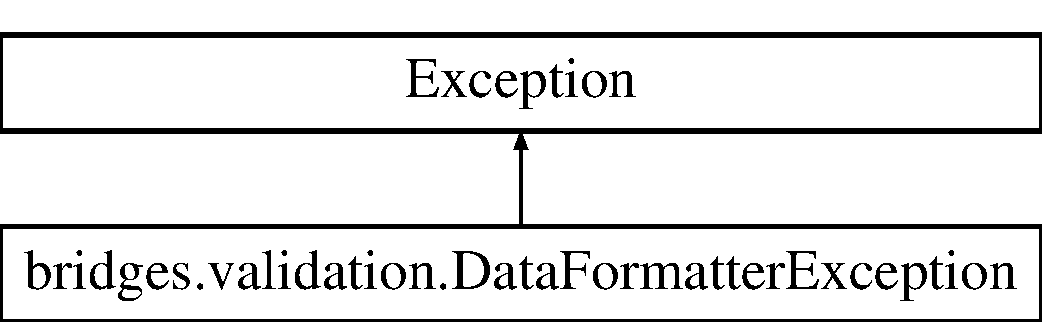
\includegraphics[height=2.000000cm]{classbridges_1_1validation_1_1_data_formatter_exception}
\end{center}
\end{figure}
\subsection*{Public Member Functions}
\begin{DoxyCompactItemize}
\item 
\hyperlink{classbridges_1_1validation_1_1_data_formatter_exception_aa922b9fa359b89c0b25eaa1efd0cfd07}{Data\+Formatter\+Exception} ()
\item 
\hyperlink{classbridges_1_1validation_1_1_data_formatter_exception_abadd66eb3ea98c1af1ff397912ed73bf}{Data\+Formatter\+Exception} (String message)
\item 
\hyperlink{classbridges_1_1validation_1_1_data_formatter_exception_ae7ce6479c3caf8077d5e34b79fe980dd}{Data\+Formatter\+Exception} (Throwable cause)
\item 
\hyperlink{classbridges_1_1validation_1_1_data_formatter_exception_acaec0fe0a826d08481207a3bac21c913}{Data\+Formatter\+Exception} (String message, Throwable cause)
\item 
String \hyperlink{classbridges_1_1validation_1_1_data_formatter_exception_ad60457ab04769d2c80e6ba77a6307ce1}{get\+Error} ()
\item 
Throwable \hyperlink{classbridges_1_1validation_1_1_data_formatter_exception_a6223e92ea95f3050d532997cb115cf2a}{get\+Cause} ()
\end{DoxyCompactItemize}
\subsection*{Public Attributes}
\begin{DoxyCompactItemize}
\item 
String \hyperlink{classbridges_1_1validation_1_1_data_formatter_exception_a8cab4688a8a80a0575bcda28e6ac7b8c}{a\+Message}
\item 
Throwable \hyperlink{classbridges_1_1validation_1_1_data_formatter_exception_ad2fdeb878690d9fc23f1316f55696ffd}{a\+Cause}
\end{DoxyCompactItemize}


\subsection{Detailed Description}
This is an extension of the Exception class adding my customized exceptions \begin{DoxyAuthor}{Author}
mihai 
\end{DoxyAuthor}


\subsection{Constructor \& Destructor Documentation}
\hypertarget{classbridges_1_1validation_1_1_data_formatter_exception_aa922b9fa359b89c0b25eaa1efd0cfd07}{}\label{classbridges_1_1validation_1_1_data_formatter_exception_aa922b9fa359b89c0b25eaa1efd0cfd07} 
\index{bridges\+::validation\+::\+Data\+Formatter\+Exception@{bridges\+::validation\+::\+Data\+Formatter\+Exception}!Data\+Formatter\+Exception@{Data\+Formatter\+Exception}}
\index{Data\+Formatter\+Exception@{Data\+Formatter\+Exception}!bridges\+::validation\+::\+Data\+Formatter\+Exception@{bridges\+::validation\+::\+Data\+Formatter\+Exception}}
\subsubsection{\texorpdfstring{Data\+Formatter\+Exception()}{DataFormatterException()}\hspace{0.1cm}{\footnotesize\ttfamily [1/4]}}
{\footnotesize\ttfamily bridges.\+validation.\+Data\+Formatter\+Exception.\+Data\+Formatter\+Exception (\begin{DoxyParamCaption}{ }\end{DoxyParamCaption})}

\hypertarget{classbridges_1_1validation_1_1_data_formatter_exception_abadd66eb3ea98c1af1ff397912ed73bf}{}\label{classbridges_1_1validation_1_1_data_formatter_exception_abadd66eb3ea98c1af1ff397912ed73bf} 
\index{bridges\+::validation\+::\+Data\+Formatter\+Exception@{bridges\+::validation\+::\+Data\+Formatter\+Exception}!Data\+Formatter\+Exception@{Data\+Formatter\+Exception}}
\index{Data\+Formatter\+Exception@{Data\+Formatter\+Exception}!bridges\+::validation\+::\+Data\+Formatter\+Exception@{bridges\+::validation\+::\+Data\+Formatter\+Exception}}
\subsubsection{\texorpdfstring{Data\+Formatter\+Exception()}{DataFormatterException()}\hspace{0.1cm}{\footnotesize\ttfamily [2/4]}}
{\footnotesize\ttfamily bridges.\+validation.\+Data\+Formatter\+Exception.\+Data\+Formatter\+Exception (\begin{DoxyParamCaption}\item[{String}]{message }\end{DoxyParamCaption})}

\hypertarget{classbridges_1_1validation_1_1_data_formatter_exception_ae7ce6479c3caf8077d5e34b79fe980dd}{}\label{classbridges_1_1validation_1_1_data_formatter_exception_ae7ce6479c3caf8077d5e34b79fe980dd} 
\index{bridges\+::validation\+::\+Data\+Formatter\+Exception@{bridges\+::validation\+::\+Data\+Formatter\+Exception}!Data\+Formatter\+Exception@{Data\+Formatter\+Exception}}
\index{Data\+Formatter\+Exception@{Data\+Formatter\+Exception}!bridges\+::validation\+::\+Data\+Formatter\+Exception@{bridges\+::validation\+::\+Data\+Formatter\+Exception}}
\subsubsection{\texorpdfstring{Data\+Formatter\+Exception()}{DataFormatterException()}\hspace{0.1cm}{\footnotesize\ttfamily [3/4]}}
{\footnotesize\ttfamily bridges.\+validation.\+Data\+Formatter\+Exception.\+Data\+Formatter\+Exception (\begin{DoxyParamCaption}\item[{Throwable}]{cause }\end{DoxyParamCaption})}

\hypertarget{classbridges_1_1validation_1_1_data_formatter_exception_acaec0fe0a826d08481207a3bac21c913}{}\label{classbridges_1_1validation_1_1_data_formatter_exception_acaec0fe0a826d08481207a3bac21c913} 
\index{bridges\+::validation\+::\+Data\+Formatter\+Exception@{bridges\+::validation\+::\+Data\+Formatter\+Exception}!Data\+Formatter\+Exception@{Data\+Formatter\+Exception}}
\index{Data\+Formatter\+Exception@{Data\+Formatter\+Exception}!bridges\+::validation\+::\+Data\+Formatter\+Exception@{bridges\+::validation\+::\+Data\+Formatter\+Exception}}
\subsubsection{\texorpdfstring{Data\+Formatter\+Exception()}{DataFormatterException()}\hspace{0.1cm}{\footnotesize\ttfamily [4/4]}}
{\footnotesize\ttfamily bridges.\+validation.\+Data\+Formatter\+Exception.\+Data\+Formatter\+Exception (\begin{DoxyParamCaption}\item[{String}]{message,  }\item[{Throwable}]{cause }\end{DoxyParamCaption})}



\subsection{Member Function Documentation}
\hypertarget{classbridges_1_1validation_1_1_data_formatter_exception_a6223e92ea95f3050d532997cb115cf2a}{}\label{classbridges_1_1validation_1_1_data_formatter_exception_a6223e92ea95f3050d532997cb115cf2a} 
\index{bridges\+::validation\+::\+Data\+Formatter\+Exception@{bridges\+::validation\+::\+Data\+Formatter\+Exception}!get\+Cause@{get\+Cause}}
\index{get\+Cause@{get\+Cause}!bridges\+::validation\+::\+Data\+Formatter\+Exception@{bridges\+::validation\+::\+Data\+Formatter\+Exception}}
\subsubsection{\texorpdfstring{get\+Cause()}{getCause()}}
{\footnotesize\ttfamily Throwable bridges.\+validation.\+Data\+Formatter\+Exception.\+get\+Cause (\begin{DoxyParamCaption}{ }\end{DoxyParamCaption})}

\hypertarget{classbridges_1_1validation_1_1_data_formatter_exception_ad60457ab04769d2c80e6ba77a6307ce1}{}\label{classbridges_1_1validation_1_1_data_formatter_exception_ad60457ab04769d2c80e6ba77a6307ce1} 
\index{bridges\+::validation\+::\+Data\+Formatter\+Exception@{bridges\+::validation\+::\+Data\+Formatter\+Exception}!get\+Error@{get\+Error}}
\index{get\+Error@{get\+Error}!bridges\+::validation\+::\+Data\+Formatter\+Exception@{bridges\+::validation\+::\+Data\+Formatter\+Exception}}
\subsubsection{\texorpdfstring{get\+Error()}{getError()}}
{\footnotesize\ttfamily String bridges.\+validation.\+Data\+Formatter\+Exception.\+get\+Error (\begin{DoxyParamCaption}{ }\end{DoxyParamCaption})}



\subsection{Member Data Documentation}
\hypertarget{classbridges_1_1validation_1_1_data_formatter_exception_ad2fdeb878690d9fc23f1316f55696ffd}{}\label{classbridges_1_1validation_1_1_data_formatter_exception_ad2fdeb878690d9fc23f1316f55696ffd} 
\index{bridges\+::validation\+::\+Data\+Formatter\+Exception@{bridges\+::validation\+::\+Data\+Formatter\+Exception}!a\+Cause@{a\+Cause}}
\index{a\+Cause@{a\+Cause}!bridges\+::validation\+::\+Data\+Formatter\+Exception@{bridges\+::validation\+::\+Data\+Formatter\+Exception}}
\subsubsection{\texorpdfstring{a\+Cause}{aCause}}
{\footnotesize\ttfamily Throwable bridges.\+validation.\+Data\+Formatter\+Exception.\+a\+Cause}

\hypertarget{classbridges_1_1validation_1_1_data_formatter_exception_a8cab4688a8a80a0575bcda28e6ac7b8c}{}\label{classbridges_1_1validation_1_1_data_formatter_exception_a8cab4688a8a80a0575bcda28e6ac7b8c} 
\index{bridges\+::validation\+::\+Data\+Formatter\+Exception@{bridges\+::validation\+::\+Data\+Formatter\+Exception}!a\+Message@{a\+Message}}
\index{a\+Message@{a\+Message}!bridges\+::validation\+::\+Data\+Formatter\+Exception@{bridges\+::validation\+::\+Data\+Formatter\+Exception}}
\subsubsection{\texorpdfstring{a\+Message}{aMessage}}
{\footnotesize\ttfamily String bridges.\+validation.\+Data\+Formatter\+Exception.\+a\+Message}



The documentation for this class was generated from the following file\+:\begin{DoxyCompactItemize}
\item 
/\+Users/kalpathi/gr/bridges/client/java/bridges16/src/main/java/edu/uncc/cs/bridges\+\_\+v21/validation/\hyperlink{_data_formatter_exception_8java}{Data\+Formatter\+Exception.\+java}\end{DoxyCompactItemize}

\hypertarget{classbridges_1_1base_1_1_data_struct}{}\section{bridges.\+base.\+Data\+Struct Class Reference}
\label{classbridges_1_1base_1_1_data_struct}\index{bridges.\+base.\+Data\+Struct@{bridges.\+base.\+Data\+Struct}}


This is an abstract super class that is extended by all Bridges subclasses and provides some methods that are used universally across B\+R\+I\+D\+G\+ES.  


Inheritance diagram for bridges.\+base.\+Data\+Struct\+:\begin{figure}[H]
\begin{center}
\leavevmode
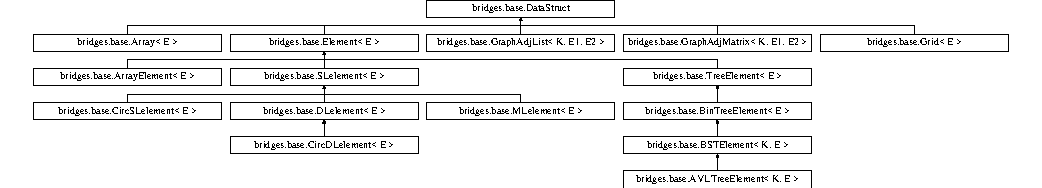
\includegraphics[height=3.485477cm]{classbridges_1_1base_1_1_data_struct}
\end{center}
\end{figure}
\subsection*{Protected Member Functions}
\begin{DoxyCompactItemize}
\item 
abstract String \hyperlink{classbridges_1_1base_1_1_data_struct_a3bae9d0d68a85e517a34be482e90fdd4}{get\+Data\+Struct\+Type} ()
\end{DoxyCompactItemize}
\subsection*{Protected Attributes}
\begin{DoxyCompactItemize}
\item 
String \hyperlink{classbridges_1_1base_1_1_data_struct_aac4a6ea28f44676274120ba1dddafc1f}{Q\+U\+O\+TE} = \char`\"{}\textbackslash{}\char`\"{}\char`\"{}
\end{DoxyCompactItemize}


\subsection{Detailed Description}
This is an abstract super class that is extended by all Bridges subclasses and provides some methods that are used universally across B\+R\+I\+D\+G\+ES. 

\subsection{Member Function Documentation}
\hypertarget{classbridges_1_1base_1_1_data_struct_a3bae9d0d68a85e517a34be482e90fdd4}{}\label{classbridges_1_1base_1_1_data_struct_a3bae9d0d68a85e517a34be482e90fdd4} 
\index{bridges\+::base\+::\+Data\+Struct@{bridges\+::base\+::\+Data\+Struct}!get\+Data\+Struct\+Type@{get\+Data\+Struct\+Type}}
\index{get\+Data\+Struct\+Type@{get\+Data\+Struct\+Type}!bridges\+::base\+::\+Data\+Struct@{bridges\+::base\+::\+Data\+Struct}}
\subsubsection{\texorpdfstring{get\+Data\+Struct\+Type()}{getDataStructType()}}
{\footnotesize\ttfamily abstract String bridges.\+base.\+Data\+Struct.\+get\+Data\+Struct\+Type (\begin{DoxyParamCaption}{ }\end{DoxyParamCaption})\hspace{0.3cm}{\ttfamily [abstract]}, {\ttfamily [protected]}}



\subsection{Member Data Documentation}
\hypertarget{classbridges_1_1base_1_1_data_struct_aac4a6ea28f44676274120ba1dddafc1f}{}\label{classbridges_1_1base_1_1_data_struct_aac4a6ea28f44676274120ba1dddafc1f} 
\index{bridges\+::base\+::\+Data\+Struct@{bridges\+::base\+::\+Data\+Struct}!Q\+U\+O\+TE@{Q\+U\+O\+TE}}
\index{Q\+U\+O\+TE@{Q\+U\+O\+TE}!bridges\+::base\+::\+Data\+Struct@{bridges\+::base\+::\+Data\+Struct}}
\subsubsection{\texorpdfstring{Q\+U\+O\+TE}{QUOTE}}
{\footnotesize\ttfamily String bridges.\+base.\+Data\+Struct.\+Q\+U\+O\+TE = \char`\"{}\textbackslash{}\char`\"{}\char`\"{}\hspace{0.3cm}{\ttfamily [protected]}}



The documentation for this class was generated from the following file\+:\begin{DoxyCompactItemize}
\item 
/\+Users/kalpathi/gr/bridges/client/java/bridges16/src/main/java/edu/uncc/cs/bridges\+\_\+v21/base/\hyperlink{_data_struct_8java}{Data\+Struct.\+java}\end{DoxyCompactItemize}

\hypertarget{classbridges_1_1base_1_1_d_lelement}{}\section{bridges.\+base.\+D\+Lelement$<$ E $>$ Class Template Reference}
\label{classbridges_1_1base_1_1_d_lelement}\index{bridges.\+base.\+D\+Lelement$<$ E $>$@{bridges.\+base.\+D\+Lelement$<$ E $>$}}


This class is used to create doubly linked element objects.  


Inheritance diagram for bridges.\+base.\+D\+Lelement$<$ E $>$\+:\begin{figure}[H]
\begin{center}
\leavevmode
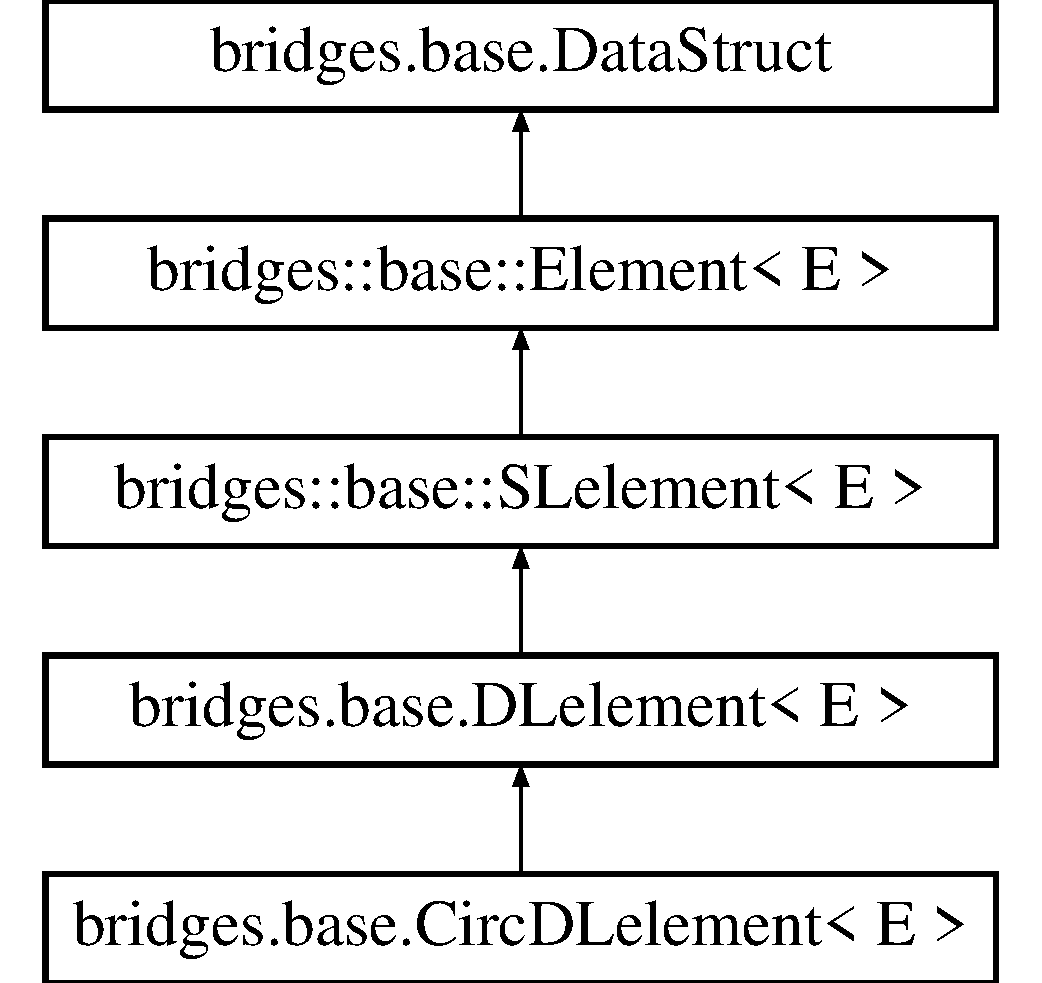
\includegraphics[height=5.000000cm]{classbridges_1_1base_1_1_d_lelement}
\end{center}
\end{figure}
\subsection*{Public Member Functions}
\begin{DoxyCompactItemize}
\item 
\hyperlink{classbridges_1_1base_1_1_d_lelement_a525b572340e161d9c430baff10b64ab2}{D\+Lelement} ()
\item 
\hyperlink{classbridges_1_1base_1_1_d_lelement_a6aa1d4a3dad4a196c2ed079d108562bc}{D\+Lelement} (String label, E e)
\item 
\hyperlink{classbridges_1_1base_1_1_d_lelement_ab1e4eace66bb1b097463c4f04e964cd0}{D\+Lelement} (\hyperlink{classbridges_1_1base_1_1_d_lelement}{D\+Lelement}$<$ E $>$ \hyperlink{classbridges_1_1base_1_1_s_lelement_abf61c96a74ad319d561c6952ea388e0e}{next}, \hyperlink{classbridges_1_1base_1_1_d_lelement}{D\+Lelement}$<$ E $>$ \hyperlink{classbridges_1_1base_1_1_d_lelement_a6eba4876f820b75ac6bde01d7dea9da7}{prev})
\item 
\hyperlink{classbridges_1_1base_1_1_d_lelement_a3ffba30204a2ea6939b07b0ded123af5}{D\+Lelement} (E e, \hyperlink{classbridges_1_1base_1_1_d_lelement}{D\+Lelement}$<$ E $>$ \hyperlink{classbridges_1_1base_1_1_s_lelement_abf61c96a74ad319d561c6952ea388e0e}{next}, \hyperlink{classbridges_1_1base_1_1_d_lelement}{D\+Lelement}$<$ E $>$ \hyperlink{classbridges_1_1base_1_1_d_lelement_a6eba4876f820b75ac6bde01d7dea9da7}{prev})
\item 
String \hyperlink{classbridges_1_1base_1_1_d_lelement_a4a0e8f7bd377a652927a741e70aae6d3}{get\+Data\+Struct\+Type} ()
\item 
\hyperlink{classbridges_1_1base_1_1_d_lelement}{D\+Lelement}$<$ E $>$ \hyperlink{classbridges_1_1base_1_1_d_lelement_a35e88e8d991d6f23ec63b3ef3f6cce4e}{get\+Next} ()
\item 
\hyperlink{classbridges_1_1base_1_1_d_lelement}{D\+Lelement}$<$ E $>$ \hyperlink{classbridges_1_1base_1_1_d_lelement_a859f08f38513ecdfff0eb11bd2b98ce7}{get\+Prev} ()
\item 
void \hyperlink{classbridges_1_1base_1_1_d_lelement_a152a06add922290d48b2d4affc87d592}{set\+Prev} (\hyperlink{classbridges_1_1base_1_1_d_lelement}{D\+Lelement}$<$ E $>$ prv)
\item 
String \hyperlink{classbridges_1_1base_1_1_d_lelement_aefe2e582992a9e574d733f109add80f2}{get\+Data\+Structure\+Representation} ()
\end{DoxyCompactItemize}
\subsection*{Protected Attributes}
\begin{DoxyCompactItemize}
\item 
\hyperlink{classbridges_1_1base_1_1_d_lelement}{D\+Lelement}$<$ E $>$ \hyperlink{classbridges_1_1base_1_1_d_lelement_a6eba4876f820b75ac6bde01d7dea9da7}{prev}
\end{DoxyCompactItemize}
\subsection*{Additional Inherited Members}


\subsection{Detailed Description}
This class is used to create doubly linked element objects. 

\begin{DoxyAuthor}{Author}
Mihai Mehedint, Kalpathi Subramanian
\end{DoxyAuthor}
\begin{DoxyDate}{Date}
6/22/16, 1/7/17, 5/17/17
\end{DoxyDate}
This class extends \hyperlink{classbridges_1_1base_1_1_element}{Element} and takes a generic parameter $<$\+E$>$ representing application specific data. This element forms the basic building block for doubly linked lists. Doubly linked elements have two links, \char`\"{}next\char`\"{} and \char`\"{}previous\char`\"{}, that point to the previous and succeeding nodes along the list.

Elements contain a visualizer (\hyperlink{classbridges_1_1base_1_1_element_visualizer}{Element\+Visualizer}) object for setting visual attributes (color, shape, opacity, size), necessary for displaying them in a web browser.

Elements also have a \hyperlink{classbridges_1_1base_1_1_link_visualizer}{Link\+Visualizer} object that is used when they are linked to another element, appropriate for setting link attributes, such as in linked lists, between the current element and its next or previous nodes.


\begin{DoxyParams}{Parameters}
{\em $<$\+E$>$} & The generic parameter object that is part of this element, representing application specific data.\\
\hline
\end{DoxyParams}
\begin{DoxySeeAlso}{See also}
Example Tutorial at ~\newline
 \href{http://bridgesuncc.github.io/Hello_World_Tutorials/DLL.html}{\tt http\+://bridgesuncc.\+github.\+io/\+Hello\+\_\+\+World\+\_\+\+Tutorials/\+D\+L\+L.\+html} 
\end{DoxySeeAlso}


\subsection{Constructor \& Destructor Documentation}
\hypertarget{classbridges_1_1base_1_1_d_lelement_a525b572340e161d9c430baff10b64ab2}{}\index{bridges\+::base\+::\+D\+Lelement@{bridges\+::base\+::\+D\+Lelement}!D\+Lelement@{D\+Lelement}}
\index{D\+Lelement@{D\+Lelement}!bridges\+::base\+::\+D\+Lelement@{bridges\+::base\+::\+D\+Lelement}}
\subsubsection[{D\+Lelement()}]{\setlength{\rightskip}{0pt plus 5cm}{\bf bridges.\+base.\+D\+Lelement}$<$ E $>$.{\bf D\+Lelement} (
\begin{DoxyParamCaption}
{}
\end{DoxyParamCaption}
)}\label{classbridges_1_1base_1_1_d_lelement_a525b572340e161d9c430baff10b64ab2}
Constructs an empty \hyperlink{classbridges_1_1base_1_1_d_lelement}{D\+Lelement} with next and prev pointers set to null. \hypertarget{classbridges_1_1base_1_1_d_lelement_a6aa1d4a3dad4a196c2ed079d108562bc}{}\index{bridges\+::base\+::\+D\+Lelement@{bridges\+::base\+::\+D\+Lelement}!D\+Lelement@{D\+Lelement}}
\index{D\+Lelement@{D\+Lelement}!bridges\+::base\+::\+D\+Lelement@{bridges\+::base\+::\+D\+Lelement}}
\subsubsection[{D\+Lelement(\+String label, E e)}]{\setlength{\rightskip}{0pt plus 5cm}{\bf bridges.\+base.\+D\+Lelement}$<$ E $>$.{\bf D\+Lelement} (
\begin{DoxyParamCaption}
\item[{String}]{label, }
\item[{E}]{e}
\end{DoxyParamCaption}
)}\label{classbridges_1_1base_1_1_d_lelement_a6aa1d4a3dad4a196c2ed079d108562bc}
Constructs a \hyperlink{classbridges_1_1base_1_1_d_lelement}{D\+Lelement} labeled \char`\"{}label\char`\"{}, holding an object \char`\"{}e\char`\"{}, with next and prev pointers set to null.


\begin{DoxyParams}{Parameters}
{\em label} & the label for this \hyperlink{classbridges_1_1base_1_1_d_lelement}{D\+Lelement} that shows up on the Bridges visualization \\
\hline
{\em e} & the genereic object that is held in this element. \\
\hline
\end{DoxyParams}
\hypertarget{classbridges_1_1base_1_1_d_lelement_ab1e4eace66bb1b097463c4f04e964cd0}{}\index{bridges\+::base\+::\+D\+Lelement@{bridges\+::base\+::\+D\+Lelement}!D\+Lelement@{D\+Lelement}}
\index{D\+Lelement@{D\+Lelement}!bridges\+::base\+::\+D\+Lelement@{bridges\+::base\+::\+D\+Lelement}}
\subsubsection[{D\+Lelement(\+D\+Lelement$<$ E $>$ next, D\+Lelement$<$ E $>$ prev)}]{\setlength{\rightskip}{0pt plus 5cm}{\bf bridges.\+base.\+D\+Lelement}$<$ E $>$.{\bf D\+Lelement} (
\begin{DoxyParamCaption}
\item[{{\bf D\+Lelement}$<$ E $>$}]{next, }
\item[{{\bf D\+Lelement}$<$ E $>$}]{prev}
\end{DoxyParamCaption}
)}\label{classbridges_1_1base_1_1_d_lelement_ab1e4eace66bb1b097463c4f04e964cd0}
Constructs an empty \hyperlink{classbridges_1_1base_1_1_d_lelement}{D\+Lelement} with the next pointer set to the \hyperlink{classbridges_1_1base_1_1_d_lelement}{D\+Lelement} \char`\"{}next\char`\"{} and the prev pointer set to \hyperlink{classbridges_1_1base_1_1_d_lelement}{D\+Lelement} \char`\"{}prev\char`\"{}.


\begin{DoxyParams}{Parameters}
{\em next} & the \hyperlink{classbridges_1_1base_1_1_d_lelement}{D\+Lelement} that should be assigned to the next pointer \\
\hline
{\em prev} & the \hyperlink{classbridges_1_1base_1_1_d_lelement}{D\+Lelement} that should be assigned to the prev pointer \\
\hline
\end{DoxyParams}
\hypertarget{classbridges_1_1base_1_1_d_lelement_a3ffba30204a2ea6939b07b0ded123af5}{}\index{bridges\+::base\+::\+D\+Lelement@{bridges\+::base\+::\+D\+Lelement}!D\+Lelement@{D\+Lelement}}
\index{D\+Lelement@{D\+Lelement}!bridges\+::base\+::\+D\+Lelement@{bridges\+::base\+::\+D\+Lelement}}
\subsubsection[{D\+Lelement(\+E e, D\+Lelement$<$ E $>$ next, D\+Lelement$<$ E $>$ prev)}]{\setlength{\rightskip}{0pt plus 5cm}{\bf bridges.\+base.\+D\+Lelement}$<$ E $>$.{\bf D\+Lelement} (
\begin{DoxyParamCaption}
\item[{E}]{e, }
\item[{{\bf D\+Lelement}$<$ E $>$}]{next, }
\item[{{\bf D\+Lelement}$<$ E $>$}]{prev}
\end{DoxyParamCaption}
)}\label{classbridges_1_1base_1_1_d_lelement_a3ffba30204a2ea6939b07b0ded123af5}
Constructs a \hyperlink{classbridges_1_1base_1_1_d_lelement}{D\+Lelement} holding an object \char`\"{}e\char`\"{}, with the next pointer set to the \hyperlink{classbridges_1_1base_1_1_d_lelement}{D\+Lelement} \char`\"{}next\char`\"{} and the prev pointer set to \hyperlink{classbridges_1_1base_1_1_d_lelement}{D\+Lelement} \char`\"{}prev\char`\"{}.


\begin{DoxyParams}{Parameters}
{\em e} & the genereic object that this \hyperlink{classbridges_1_1base_1_1_d_lelement}{D\+Lelement} is holding \\
\hline
{\em next} & the \hyperlink{classbridges_1_1base_1_1_d_lelement}{D\+Lelement} that should be assigned to the next pointer \\
\hline
{\em prev} & the \hyperlink{classbridges_1_1base_1_1_d_lelement}{D\+Lelement} that should be assigned to the prev pointer \\
\hline
\end{DoxyParams}


\subsection{Member Function Documentation}
\hypertarget{classbridges_1_1base_1_1_d_lelement_a4a0e8f7bd377a652927a741e70aae6d3}{}\index{bridges\+::base\+::\+D\+Lelement@{bridges\+::base\+::\+D\+Lelement}!get\+Data\+Struct\+Type@{get\+Data\+Struct\+Type}}
\index{get\+Data\+Struct\+Type@{get\+Data\+Struct\+Type}!bridges\+::base\+::\+D\+Lelement@{bridges\+::base\+::\+D\+Lelement}}
\subsubsection[{get\+Data\+Struct\+Type()}]{\setlength{\rightskip}{0pt plus 5cm}String {\bf bridges.\+base.\+D\+Lelement}$<$ E $>$.get\+Data\+Struct\+Type (
\begin{DoxyParamCaption}
{}
\end{DoxyParamCaption}
)}\label{classbridges_1_1base_1_1_d_lelement_a4a0e8f7bd377a652927a741e70aae6d3}
This method gets the data structure type

\begin{DoxyReturn}{Returns}
The date structure type as a string 
\end{DoxyReturn}
\hypertarget{classbridges_1_1base_1_1_d_lelement_aefe2e582992a9e574d733f109add80f2}{}\index{bridges\+::base\+::\+D\+Lelement@{bridges\+::base\+::\+D\+Lelement}!get\+Data\+Structure\+Representation@{get\+Data\+Structure\+Representation}}
\index{get\+Data\+Structure\+Representation@{get\+Data\+Structure\+Representation}!bridges\+::base\+::\+D\+Lelement@{bridges\+::base\+::\+D\+Lelement}}
\subsubsection[{get\+Data\+Structure\+Representation()}]{\setlength{\rightskip}{0pt plus 5cm}String {\bf bridges.\+base.\+D\+Lelement}$<$ E $>$.get\+Data\+Structure\+Representation (
\begin{DoxyParamCaption}
{}
\end{DoxyParamCaption}
)}\label{classbridges_1_1base_1_1_d_lelement_aefe2e582992a9e574d733f109add80f2}
\hypertarget{classbridges_1_1base_1_1_d_lelement_a35e88e8d991d6f23ec63b3ef3f6cce4e}{}\index{bridges\+::base\+::\+D\+Lelement@{bridges\+::base\+::\+D\+Lelement}!get\+Next@{get\+Next}}
\index{get\+Next@{get\+Next}!bridges\+::base\+::\+D\+Lelement@{bridges\+::base\+::\+D\+Lelement}}
\subsubsection[{get\+Next()}]{\setlength{\rightskip}{0pt plus 5cm}{\bf D\+Lelement}$<$E$>$ {\bf bridges.\+base.\+D\+Lelement}$<$ E $>$.get\+Next (
\begin{DoxyParamCaption}
{}
\end{DoxyParamCaption}
)}\label{classbridges_1_1base_1_1_d_lelement_a35e88e8d991d6f23ec63b3ef3f6cce4e}
This method returns the pointer to the next \hyperlink{classbridges_1_1base_1_1_d_lelement}{D\+Lelement}

\begin{DoxyReturn}{Returns}
the \hyperlink{classbridges_1_1base_1_1_d_lelement}{D\+Lelement} assigned to the next pointer 
\end{DoxyReturn}
\hypertarget{classbridges_1_1base_1_1_d_lelement_a859f08f38513ecdfff0eb11bd2b98ce7}{}\index{bridges\+::base\+::\+D\+Lelement@{bridges\+::base\+::\+D\+Lelement}!get\+Prev@{get\+Prev}}
\index{get\+Prev@{get\+Prev}!bridges\+::base\+::\+D\+Lelement@{bridges\+::base\+::\+D\+Lelement}}
\subsubsection[{get\+Prev()}]{\setlength{\rightskip}{0pt plus 5cm}{\bf D\+Lelement}$<$E$>$ {\bf bridges.\+base.\+D\+Lelement}$<$ E $>$.get\+Prev (
\begin{DoxyParamCaption}
{}
\end{DoxyParamCaption}
)}\label{classbridges_1_1base_1_1_d_lelement_a859f08f38513ecdfff0eb11bd2b98ce7}
This method sets the pointer to the next \hyperlink{classbridges_1_1base_1_1_d_lelement}{D\+Lelement}


\begin{DoxyParams}{Parameters}
{\em next} & the \hyperlink{classbridges_1_1base_1_1_d_lelement}{D\+Lelement} that should be assigned to the next pointer This method returns the pointer to the previous \hyperlink{classbridges_1_1base_1_1_d_lelement}{D\+Lelement}\\
\hline
\end{DoxyParams}
\begin{DoxyReturn}{Returns}
the \hyperlink{classbridges_1_1base_1_1_d_lelement}{D\+Lelement} assigned to the prev pointer 
\end{DoxyReturn}
\hypertarget{classbridges_1_1base_1_1_d_lelement_a152a06add922290d48b2d4affc87d592}{}\index{bridges\+::base\+::\+D\+Lelement@{bridges\+::base\+::\+D\+Lelement}!set\+Prev@{set\+Prev}}
\index{set\+Prev@{set\+Prev}!bridges\+::base\+::\+D\+Lelement@{bridges\+::base\+::\+D\+Lelement}}
\subsubsection[{set\+Prev(\+D\+Lelement$<$ E $>$ prv)}]{\setlength{\rightskip}{0pt plus 5cm}void {\bf bridges.\+base.\+D\+Lelement}$<$ E $>$.set\+Prev (
\begin{DoxyParamCaption}
\item[{{\bf D\+Lelement}$<$ E $>$}]{prv}
\end{DoxyParamCaption}
)}\label{classbridges_1_1base_1_1_d_lelement_a152a06add922290d48b2d4affc87d592}
This method sets the pointer to the previous \hyperlink{classbridges_1_1base_1_1_d_lelement}{D\+Lelement}


\begin{DoxyParams}{Parameters}
{\em prev} & the \hyperlink{classbridges_1_1base_1_1_d_lelement}{D\+Lelement} that should be assigned to the prev pointer \\
\hline
\end{DoxyParams}


\subsection{Member Data Documentation}
\hypertarget{classbridges_1_1base_1_1_d_lelement_a6eba4876f820b75ac6bde01d7dea9da7}{}\index{bridges\+::base\+::\+D\+Lelement@{bridges\+::base\+::\+D\+Lelement}!prev@{prev}}
\index{prev@{prev}!bridges\+::base\+::\+D\+Lelement@{bridges\+::base\+::\+D\+Lelement}}
\subsubsection[{prev}]{\setlength{\rightskip}{0pt plus 5cm}{\bf D\+Lelement}$<$E$>$ {\bf bridges.\+base.\+D\+Lelement}$<$ E $>$.prev\hspace{0.3cm}{\ttfamily [protected]}}\label{classbridges_1_1base_1_1_d_lelement_a6eba4876f820b75ac6bde01d7dea9da7}


The documentation for this class was generated from the following file\+:\begin{DoxyCompactItemize}
\item 
/\+Users/kalpathi/gr/bridges/bridges17/java/src/main/java/bridges/base/\hyperlink{_d_lelement_8java}{D\+Lelement.\+java}\end{DoxyCompactItemize}

\hypertarget{classbridges_1_1data__src__dependent_1_1_earthquake_tweet}{}\section{bridges.\+data\+\_\+src\+\_\+dependent.\+Earthquake\+Tweet Class Reference}
\label{classbridges_1_1data__src__dependent_1_1_earthquake_tweet}\index{bridges.\+data\+\_\+src\+\_\+dependent.\+Earthquake\+Tweet@{bridges.\+data\+\_\+src\+\_\+dependent.\+Earthquake\+Tweet}}
Inheritance diagram for bridges.\+data\+\_\+src\+\_\+dependent.\+Earthquake\+Tweet\+:\begin{figure}[H]
\begin{center}
\leavevmode
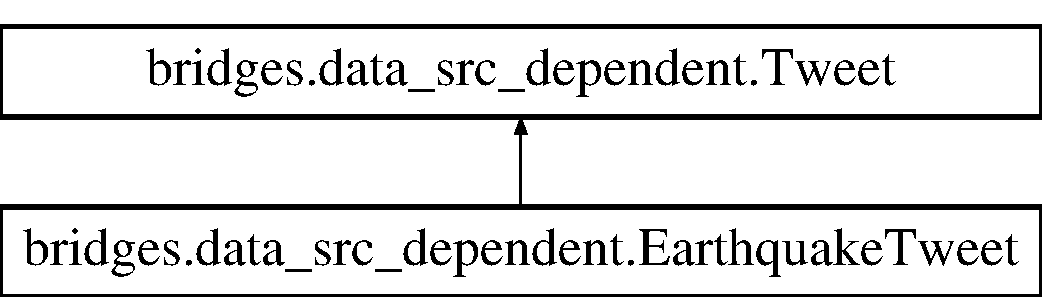
\includegraphics[height=2.000000cm]{classbridges_1_1data__src__dependent_1_1_earthquake_tweet}
\end{center}
\end{figure}
\subsection*{Public Member Functions}
\begin{DoxyCompactItemize}
\item 
\hyperlink{classbridges_1_1data__src__dependent_1_1_earthquake_tweet_a1f2d4634e85c75c59ba9d4aec878db54}{Earthquake\+Tweet} (String content, Date date2)
\item 
\hyperlink{classbridges_1_1data__src__dependent_1_1_earthquake_tweet_af0a8e9201997a7d4805f11c02f197410}{Earthquake\+Tweet} (\hyperlink{classbridges_1_1data__src__dependent_1_1_tweet}{Tweet} a\+Tweet)
\item 
void \hyperlink{classbridges_1_1data__src__dependent_1_1_earthquake_tweet_a49880f314eee430098ca347cd07ff470}{set\+Magnitude} ()
\item 
void \hyperlink{classbridges_1_1data__src__dependent_1_1_earthquake_tweet_a763d8a261a563e66af95c5a97850ecc0}{set\+Magnitude} (double mag)
\item 
String \hyperlink{classbridges_1_1data__src__dependent_1_1_earthquake_tweet_a3e39d6fa01f24cb259d32bb39108feb1}{enter\+Carriage\+Return} (String str)
\item 
double \hyperlink{classbridges_1_1data__src__dependent_1_1_earthquake_tweet_a8f3d92b4e60b922e996ecfaee3c5260e}{get\+Magnitude} ()
\item 
int \hyperlink{classbridges_1_1data__src__dependent_1_1_earthquake_tweet_a6b4de2a600b93ed96f6cde8b719ea645}{compare\+To} (Data\+Source o)
\end{DoxyCompactItemize}


\subsection{Detailed Description}
\begin{DoxyAuthor}{Author}
mihai mehedint 
\end{DoxyAuthor}


\subsection{Constructor \& Destructor Documentation}
\hypertarget{classbridges_1_1data__src__dependent_1_1_earthquake_tweet_a1f2d4634e85c75c59ba9d4aec878db54}{}\index{bridges\+::data\+\_\+src\+\_\+dependent\+::\+Earthquake\+Tweet@{bridges\+::data\+\_\+src\+\_\+dependent\+::\+Earthquake\+Tweet}!Earthquake\+Tweet@{Earthquake\+Tweet}}
\index{Earthquake\+Tweet@{Earthquake\+Tweet}!bridges\+::data\+\_\+src\+\_\+dependent\+::\+Earthquake\+Tweet@{bridges\+::data\+\_\+src\+\_\+dependent\+::\+Earthquake\+Tweet}}
\subsubsection[{Earthquake\+Tweet(\+String content, Date date2)}]{\setlength{\rightskip}{0pt plus 5cm}bridges.\+data\+\_\+src\+\_\+dependent.\+Earthquake\+Tweet.\+Earthquake\+Tweet (
\begin{DoxyParamCaption}
\item[{String}]{content, }
\item[{Date}]{date2}
\end{DoxyParamCaption}
)}\label{classbridges_1_1data__src__dependent_1_1_earthquake_tweet_a1f2d4634e85c75c59ba9d4aec878db54}
\hypertarget{classbridges_1_1data__src__dependent_1_1_earthquake_tweet_af0a8e9201997a7d4805f11c02f197410}{}\index{bridges\+::data\+\_\+src\+\_\+dependent\+::\+Earthquake\+Tweet@{bridges\+::data\+\_\+src\+\_\+dependent\+::\+Earthquake\+Tweet}!Earthquake\+Tweet@{Earthquake\+Tweet}}
\index{Earthquake\+Tweet@{Earthquake\+Tweet}!bridges\+::data\+\_\+src\+\_\+dependent\+::\+Earthquake\+Tweet@{bridges\+::data\+\_\+src\+\_\+dependent\+::\+Earthquake\+Tweet}}
\subsubsection[{Earthquake\+Tweet(\+Tweet a\+Tweet)}]{\setlength{\rightskip}{0pt plus 5cm}bridges.\+data\+\_\+src\+\_\+dependent.\+Earthquake\+Tweet.\+Earthquake\+Tweet (
\begin{DoxyParamCaption}
\item[{{\bf Tweet}}]{a\+Tweet}
\end{DoxyParamCaption}
)}\label{classbridges_1_1data__src__dependent_1_1_earthquake_tweet_af0a8e9201997a7d4805f11c02f197410}


\subsection{Member Function Documentation}
\hypertarget{classbridges_1_1data__src__dependent_1_1_earthquake_tweet_a6b4de2a600b93ed96f6cde8b719ea645}{}\index{bridges\+::data\+\_\+src\+\_\+dependent\+::\+Earthquake\+Tweet@{bridges\+::data\+\_\+src\+\_\+dependent\+::\+Earthquake\+Tweet}!compare\+To@{compare\+To}}
\index{compare\+To@{compare\+To}!bridges\+::data\+\_\+src\+\_\+dependent\+::\+Earthquake\+Tweet@{bridges\+::data\+\_\+src\+\_\+dependent\+::\+Earthquake\+Tweet}}
\subsubsection[{compare\+To(\+Data\+Source o)}]{\setlength{\rightskip}{0pt plus 5cm}int bridges.\+data\+\_\+src\+\_\+dependent.\+Earthquake\+Tweet.\+compare\+To (
\begin{DoxyParamCaption}
\item[{Data\+Source}]{o}
\end{DoxyParamCaption}
)}\label{classbridges_1_1data__src__dependent_1_1_earthquake_tweet_a6b4de2a600b93ed96f6cde8b719ea645}
\hypertarget{classbridges_1_1data__src__dependent_1_1_earthquake_tweet_a3e39d6fa01f24cb259d32bb39108feb1}{}\index{bridges\+::data\+\_\+src\+\_\+dependent\+::\+Earthquake\+Tweet@{bridges\+::data\+\_\+src\+\_\+dependent\+::\+Earthquake\+Tweet}!enter\+Carriage\+Return@{enter\+Carriage\+Return}}
\index{enter\+Carriage\+Return@{enter\+Carriage\+Return}!bridges\+::data\+\_\+src\+\_\+dependent\+::\+Earthquake\+Tweet@{bridges\+::data\+\_\+src\+\_\+dependent\+::\+Earthquake\+Tweet}}
\subsubsection[{enter\+Carriage\+Return(\+String str)}]{\setlength{\rightskip}{0pt plus 5cm}String bridges.\+data\+\_\+src\+\_\+dependent.\+Earthquake\+Tweet.\+enter\+Carriage\+Return (
\begin{DoxyParamCaption}
\item[{String}]{str}
\end{DoxyParamCaption}
)}\label{classbridges_1_1data__src__dependent_1_1_earthquake_tweet_a3e39d6fa01f24cb259d32bb39108feb1}
\hypertarget{classbridges_1_1data__src__dependent_1_1_earthquake_tweet_a8f3d92b4e60b922e996ecfaee3c5260e}{}\index{bridges\+::data\+\_\+src\+\_\+dependent\+::\+Earthquake\+Tweet@{bridges\+::data\+\_\+src\+\_\+dependent\+::\+Earthquake\+Tweet}!get\+Magnitude@{get\+Magnitude}}
\index{get\+Magnitude@{get\+Magnitude}!bridges\+::data\+\_\+src\+\_\+dependent\+::\+Earthquake\+Tweet@{bridges\+::data\+\_\+src\+\_\+dependent\+::\+Earthquake\+Tweet}}
\subsubsection[{get\+Magnitude()}]{\setlength{\rightskip}{0pt plus 5cm}double bridges.\+data\+\_\+src\+\_\+dependent.\+Earthquake\+Tweet.\+get\+Magnitude (
\begin{DoxyParamCaption}
{}
\end{DoxyParamCaption}
)}\label{classbridges_1_1data__src__dependent_1_1_earthquake_tweet_a8f3d92b4e60b922e996ecfaee3c5260e}
\hypertarget{classbridges_1_1data__src__dependent_1_1_earthquake_tweet_a49880f314eee430098ca347cd07ff470}{}\index{bridges\+::data\+\_\+src\+\_\+dependent\+::\+Earthquake\+Tweet@{bridges\+::data\+\_\+src\+\_\+dependent\+::\+Earthquake\+Tweet}!set\+Magnitude@{set\+Magnitude}}
\index{set\+Magnitude@{set\+Magnitude}!bridges\+::data\+\_\+src\+\_\+dependent\+::\+Earthquake\+Tweet@{bridges\+::data\+\_\+src\+\_\+dependent\+::\+Earthquake\+Tweet}}
\subsubsection[{set\+Magnitude()}]{\setlength{\rightskip}{0pt plus 5cm}void bridges.\+data\+\_\+src\+\_\+dependent.\+Earthquake\+Tweet.\+set\+Magnitude (
\begin{DoxyParamCaption}
{}
\end{DoxyParamCaption}
)}\label{classbridges_1_1data__src__dependent_1_1_earthquake_tweet_a49880f314eee430098ca347cd07ff470}
\hypertarget{classbridges_1_1data__src__dependent_1_1_earthquake_tweet_a763d8a261a563e66af95c5a97850ecc0}{}\index{bridges\+::data\+\_\+src\+\_\+dependent\+::\+Earthquake\+Tweet@{bridges\+::data\+\_\+src\+\_\+dependent\+::\+Earthquake\+Tweet}!set\+Magnitude@{set\+Magnitude}}
\index{set\+Magnitude@{set\+Magnitude}!bridges\+::data\+\_\+src\+\_\+dependent\+::\+Earthquake\+Tweet@{bridges\+::data\+\_\+src\+\_\+dependent\+::\+Earthquake\+Tweet}}
\subsubsection[{set\+Magnitude(double mag)}]{\setlength{\rightskip}{0pt plus 5cm}void bridges.\+data\+\_\+src\+\_\+dependent.\+Earthquake\+Tweet.\+set\+Magnitude (
\begin{DoxyParamCaption}
\item[{double}]{mag}
\end{DoxyParamCaption}
)}\label{classbridges_1_1data__src__dependent_1_1_earthquake_tweet_a763d8a261a563e66af95c5a97850ecc0}


The documentation for this class was generated from the following file\+:\begin{DoxyCompactItemize}
\item 
/\+Users/kalpathi/gr/bridges/bridges17/java/src/main/java/bridges/data\+\_\+src\+\_\+dependent/\hyperlink{_earthquake_tweet_8java}{Earthquake\+Tweet.\+java}\end{DoxyCompactItemize}

\hypertarget{classbridges_1_1data__src__dependent_1_1_earthquake_u_s_g_s}{}\section{bridges.\+data\+\_\+src\+\_\+dependent.\+Earthquake\+U\+S\+G\+S Class Reference}
\label{classbridges_1_1data__src__dependent_1_1_earthquake_u_s_g_s}\index{bridges.\+data\+\_\+src\+\_\+dependent.\+Earthquake\+U\+S\+G\+S@{bridges.\+data\+\_\+src\+\_\+dependent.\+Earthquake\+U\+S\+G\+S}}
Inheritance diagram for bridges.\+data\+\_\+src\+\_\+dependent.\+Earthquake\+U\+S\+G\+S\+:\begin{figure}[H]
\begin{center}
\leavevmode
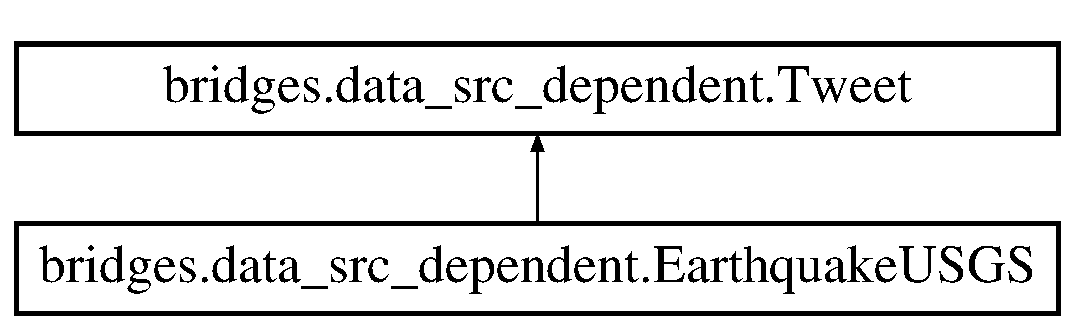
\includegraphics[height=2.000000cm]{classbridges_1_1data__src__dependent_1_1_earthquake_u_s_g_s}
\end{center}
\end{figure}
\subsection*{Public Member Functions}
\begin{DoxyCompactItemize}
\item 
\hyperlink{classbridges_1_1data__src__dependent_1_1_earthquake_u_s_g_s_a1803f7d357ce045cefbc923e096e9646}{Earthquake\+U\+S\+G\+S} ()
\item 
\hyperlink{classbridges_1_1data__src__dependent_1_1_earthquake_u_s_g_s_a767aa387d5ce45c98ad01394e0937abe}{Earthquake\+U\+S\+G\+S} (String content, Date date2, double magnitude, double longit, double latit, String location, String title, String url, String properties)
\item 
String \hyperlink{classbridges_1_1data__src__dependent_1_1_earthquake_u_s_g_s_a6676a3f0a11accf6a510648601e05310}{get\+Properties} ()
\item 
void \hyperlink{classbridges_1_1data__src__dependent_1_1_earthquake_u_s_g_s_a2e1ee813dc91081bbd8fd8f5b343f080}{set\+Properties} (String properties)
\item 
double \hyperlink{classbridges_1_1data__src__dependent_1_1_earthquake_u_s_g_s_a1b702f3081df4e29427fd4261fd57b42}{get\+Latit} ()
\item 
void \hyperlink{classbridges_1_1data__src__dependent_1_1_earthquake_u_s_g_s_aa8ca3a3aa511f52ba8bbae88118ede95}{set\+Latit} (double latit)
\item 
double \hyperlink{classbridges_1_1data__src__dependent_1_1_earthquake_u_s_g_s_a466f3594dfe3201ec468517067c3b3e5}{get\+Longit} ()
\item 
void \hyperlink{classbridges_1_1data__src__dependent_1_1_earthquake_u_s_g_s_a6e642131d91fb89bde4f13fe579f79c6}{set\+Longit} (double longit)
\item 
String \hyperlink{classbridges_1_1data__src__dependent_1_1_earthquake_u_s_g_s_a703492ad551b68ab6b7821646f9a92ec}{get\+Location} ()
\item 
void \hyperlink{classbridges_1_1data__src__dependent_1_1_earthquake_u_s_g_s_a473107844daa1ef938dd1b78e585185b}{set\+Location} (String location)
\item 
String \hyperlink{classbridges_1_1data__src__dependent_1_1_earthquake_u_s_g_s_a6aa71b4b565be3971c8d3dfae31cb6ed}{get\+Title} ()
\item 
void \hyperlink{classbridges_1_1data__src__dependent_1_1_earthquake_u_s_g_s_a0432f641e0089fc004c441b7239ad6a0}{set\+Title} (String title)
\item 
String \hyperlink{classbridges_1_1data__src__dependent_1_1_earthquake_u_s_g_s_a2af3938390c31096329e635510df437e}{get\+Url} ()
\item 
void \hyperlink{classbridges_1_1data__src__dependent_1_1_earthquake_u_s_g_s_aaa9d26333e7b80d0f72da58ea2ad41d1}{set\+Url} (String url)
\item 
void \hyperlink{classbridges_1_1data__src__dependent_1_1_earthquake_u_s_g_s_ad7902d80cbbe11046858db1f2792e99d}{set\+Magnitude} (double magnitude)
\item 
void \hyperlink{classbridges_1_1data__src__dependent_1_1_earthquake_u_s_g_s_ae3813930d3468eff007521f33c8e2139}{set\+Time} (String t)
\item 
String \hyperlink{classbridges_1_1data__src__dependent_1_1_earthquake_u_s_g_s_a03397a4410818546c5232f46a3d4ffc4}{get\+Time} ()
\item 
\hyperlink{classbridges_1_1data__src__dependent_1_1_earthquake_u_s_g_s_a6b9281a299d6e60736355eb8833f9e0d}{Earthquake\+U\+S\+G\+S} (\hyperlink{classbridges_1_1data__src__dependent_1_1_earthquake_u_s_g_s}{Earthquake\+U\+S\+G\+S} eq)
\item 
void \hyperlink{classbridges_1_1data__src__dependent_1_1_earthquake_u_s_g_s_acc0ba6890ee5963f88a399523f009ae4}{eq\+Properties} (String prop)
\item 
void \hyperlink{classbridges_1_1data__src__dependent_1_1_earthquake_u_s_g_s_a34a4c6ebe01c5daa7c86b3a4207d633f}{set\+Magnitude} (Double mag)
\item 
String \hyperlink{classbridges_1_1data__src__dependent_1_1_earthquake_u_s_g_s_aade0ce9a2fee927b015f5eb495c481e1}{enter\+Carriage\+Return} (String str)
\item 
double \hyperlink{classbridges_1_1data__src__dependent_1_1_earthquake_u_s_g_s_a3ec5d753277d6287b222448ff2477291}{get\+Magnitude} ()
\item 
int \hyperlink{classbridges_1_1data__src__dependent_1_1_earthquake_u_s_g_s_a60cad0a286825f77cd2900265acae982}{compare\+To} (Data\+Source o)
\end{DoxyCompactItemize}


\subsection{Detailed Description}
\begin{DoxyAuthor}{Author}
mihai mehedint 
\end{DoxyAuthor}


\subsection{Constructor \& Destructor Documentation}
\hypertarget{classbridges_1_1data__src__dependent_1_1_earthquake_u_s_g_s_a1803f7d357ce045cefbc923e096e9646}{}\index{bridges\+::data\+\_\+src\+\_\+dependent\+::\+Earthquake\+U\+S\+G\+S@{bridges\+::data\+\_\+src\+\_\+dependent\+::\+Earthquake\+U\+S\+G\+S}!Earthquake\+U\+S\+G\+S@{Earthquake\+U\+S\+G\+S}}
\index{Earthquake\+U\+S\+G\+S@{Earthquake\+U\+S\+G\+S}!bridges\+::data\+\_\+src\+\_\+dependent\+::\+Earthquake\+U\+S\+G\+S@{bridges\+::data\+\_\+src\+\_\+dependent\+::\+Earthquake\+U\+S\+G\+S}}
\subsubsection[{Earthquake\+U\+S\+G\+S()}]{\setlength{\rightskip}{0pt plus 5cm}bridges.\+data\+\_\+src\+\_\+dependent.\+Earthquake\+U\+S\+G\+S.\+Earthquake\+U\+S\+G\+S (
\begin{DoxyParamCaption}
{}
\end{DoxyParamCaption}
)}\label{classbridges_1_1data__src__dependent_1_1_earthquake_u_s_g_s_a1803f7d357ce045cefbc923e096e9646}
\hypertarget{classbridges_1_1data__src__dependent_1_1_earthquake_u_s_g_s_a767aa387d5ce45c98ad01394e0937abe}{}\index{bridges\+::data\+\_\+src\+\_\+dependent\+::\+Earthquake\+U\+S\+G\+S@{bridges\+::data\+\_\+src\+\_\+dependent\+::\+Earthquake\+U\+S\+G\+S}!Earthquake\+U\+S\+G\+S@{Earthquake\+U\+S\+G\+S}}
\index{Earthquake\+U\+S\+G\+S@{Earthquake\+U\+S\+G\+S}!bridges\+::data\+\_\+src\+\_\+dependent\+::\+Earthquake\+U\+S\+G\+S@{bridges\+::data\+\_\+src\+\_\+dependent\+::\+Earthquake\+U\+S\+G\+S}}
\subsubsection[{Earthquake\+U\+S\+G\+S(\+String content, Date date2, double magnitude, double longit, double latit, String location, String title, String url, String properties)}]{\setlength{\rightskip}{0pt plus 5cm}bridges.\+data\+\_\+src\+\_\+dependent.\+Earthquake\+U\+S\+G\+S.\+Earthquake\+U\+S\+G\+S (
\begin{DoxyParamCaption}
\item[{String}]{content, }
\item[{Date}]{date2, }
\item[{double}]{magnitude, }
\item[{double}]{longit, }
\item[{double}]{latit, }
\item[{String}]{location, }
\item[{String}]{title, }
\item[{String}]{url, }
\item[{String}]{properties}
\end{DoxyParamCaption}
)}\label{classbridges_1_1data__src__dependent_1_1_earthquake_u_s_g_s_a767aa387d5ce45c98ad01394e0937abe}
\hypertarget{classbridges_1_1data__src__dependent_1_1_earthquake_u_s_g_s_a6b9281a299d6e60736355eb8833f9e0d}{}\index{bridges\+::data\+\_\+src\+\_\+dependent\+::\+Earthquake\+U\+S\+G\+S@{bridges\+::data\+\_\+src\+\_\+dependent\+::\+Earthquake\+U\+S\+G\+S}!Earthquake\+U\+S\+G\+S@{Earthquake\+U\+S\+G\+S}}
\index{Earthquake\+U\+S\+G\+S@{Earthquake\+U\+S\+G\+S}!bridges\+::data\+\_\+src\+\_\+dependent\+::\+Earthquake\+U\+S\+G\+S@{bridges\+::data\+\_\+src\+\_\+dependent\+::\+Earthquake\+U\+S\+G\+S}}
\subsubsection[{Earthquake\+U\+S\+G\+S(\+Earthquake\+U\+S\+G\+S eq)}]{\setlength{\rightskip}{0pt plus 5cm}bridges.\+data\+\_\+src\+\_\+dependent.\+Earthquake\+U\+S\+G\+S.\+Earthquake\+U\+S\+G\+S (
\begin{DoxyParamCaption}
\item[{{\bf Earthquake\+U\+S\+G\+S}}]{eq}
\end{DoxyParamCaption}
)}\label{classbridges_1_1data__src__dependent_1_1_earthquake_u_s_g_s_a6b9281a299d6e60736355eb8833f9e0d}


\subsection{Member Function Documentation}
\hypertarget{classbridges_1_1data__src__dependent_1_1_earthquake_u_s_g_s_a60cad0a286825f77cd2900265acae982}{}\index{bridges\+::data\+\_\+src\+\_\+dependent\+::\+Earthquake\+U\+S\+G\+S@{bridges\+::data\+\_\+src\+\_\+dependent\+::\+Earthquake\+U\+S\+G\+S}!compare\+To@{compare\+To}}
\index{compare\+To@{compare\+To}!bridges\+::data\+\_\+src\+\_\+dependent\+::\+Earthquake\+U\+S\+G\+S@{bridges\+::data\+\_\+src\+\_\+dependent\+::\+Earthquake\+U\+S\+G\+S}}
\subsubsection[{compare\+To(\+Data\+Source o)}]{\setlength{\rightskip}{0pt plus 5cm}int bridges.\+data\+\_\+src\+\_\+dependent.\+Earthquake\+U\+S\+G\+S.\+compare\+To (
\begin{DoxyParamCaption}
\item[{Data\+Source}]{o}
\end{DoxyParamCaption}
)}\label{classbridges_1_1data__src__dependent_1_1_earthquake_u_s_g_s_a60cad0a286825f77cd2900265acae982}
\hypertarget{classbridges_1_1data__src__dependent_1_1_earthquake_u_s_g_s_aade0ce9a2fee927b015f5eb495c481e1}{}\index{bridges\+::data\+\_\+src\+\_\+dependent\+::\+Earthquake\+U\+S\+G\+S@{bridges\+::data\+\_\+src\+\_\+dependent\+::\+Earthquake\+U\+S\+G\+S}!enter\+Carriage\+Return@{enter\+Carriage\+Return}}
\index{enter\+Carriage\+Return@{enter\+Carriage\+Return}!bridges\+::data\+\_\+src\+\_\+dependent\+::\+Earthquake\+U\+S\+G\+S@{bridges\+::data\+\_\+src\+\_\+dependent\+::\+Earthquake\+U\+S\+G\+S}}
\subsubsection[{enter\+Carriage\+Return(\+String str)}]{\setlength{\rightskip}{0pt plus 5cm}String bridges.\+data\+\_\+src\+\_\+dependent.\+Earthquake\+U\+S\+G\+S.\+enter\+Carriage\+Return (
\begin{DoxyParamCaption}
\item[{String}]{str}
\end{DoxyParamCaption}
)}\label{classbridges_1_1data__src__dependent_1_1_earthquake_u_s_g_s_aade0ce9a2fee927b015f5eb495c481e1}
\hypertarget{classbridges_1_1data__src__dependent_1_1_earthquake_u_s_g_s_acc0ba6890ee5963f88a399523f009ae4}{}\index{bridges\+::data\+\_\+src\+\_\+dependent\+::\+Earthquake\+U\+S\+G\+S@{bridges\+::data\+\_\+src\+\_\+dependent\+::\+Earthquake\+U\+S\+G\+S}!eq\+Properties@{eq\+Properties}}
\index{eq\+Properties@{eq\+Properties}!bridges\+::data\+\_\+src\+\_\+dependent\+::\+Earthquake\+U\+S\+G\+S@{bridges\+::data\+\_\+src\+\_\+dependent\+::\+Earthquake\+U\+S\+G\+S}}
\subsubsection[{eq\+Properties(\+String prop)}]{\setlength{\rightskip}{0pt plus 5cm}void bridges.\+data\+\_\+src\+\_\+dependent.\+Earthquake\+U\+S\+G\+S.\+eq\+Properties (
\begin{DoxyParamCaption}
\item[{String}]{prop}
\end{DoxyParamCaption}
)}\label{classbridges_1_1data__src__dependent_1_1_earthquake_u_s_g_s_acc0ba6890ee5963f88a399523f009ae4}
\hypertarget{classbridges_1_1data__src__dependent_1_1_earthquake_u_s_g_s_a1b702f3081df4e29427fd4261fd57b42}{}\index{bridges\+::data\+\_\+src\+\_\+dependent\+::\+Earthquake\+U\+S\+G\+S@{bridges\+::data\+\_\+src\+\_\+dependent\+::\+Earthquake\+U\+S\+G\+S}!get\+Latit@{get\+Latit}}
\index{get\+Latit@{get\+Latit}!bridges\+::data\+\_\+src\+\_\+dependent\+::\+Earthquake\+U\+S\+G\+S@{bridges\+::data\+\_\+src\+\_\+dependent\+::\+Earthquake\+U\+S\+G\+S}}
\subsubsection[{get\+Latit()}]{\setlength{\rightskip}{0pt plus 5cm}double bridges.\+data\+\_\+src\+\_\+dependent.\+Earthquake\+U\+S\+G\+S.\+get\+Latit (
\begin{DoxyParamCaption}
{}
\end{DoxyParamCaption}
)}\label{classbridges_1_1data__src__dependent_1_1_earthquake_u_s_g_s_a1b702f3081df4e29427fd4261fd57b42}
\hypertarget{classbridges_1_1data__src__dependent_1_1_earthquake_u_s_g_s_a703492ad551b68ab6b7821646f9a92ec}{}\index{bridges\+::data\+\_\+src\+\_\+dependent\+::\+Earthquake\+U\+S\+G\+S@{bridges\+::data\+\_\+src\+\_\+dependent\+::\+Earthquake\+U\+S\+G\+S}!get\+Location@{get\+Location}}
\index{get\+Location@{get\+Location}!bridges\+::data\+\_\+src\+\_\+dependent\+::\+Earthquake\+U\+S\+G\+S@{bridges\+::data\+\_\+src\+\_\+dependent\+::\+Earthquake\+U\+S\+G\+S}}
\subsubsection[{get\+Location()}]{\setlength{\rightskip}{0pt plus 5cm}String bridges.\+data\+\_\+src\+\_\+dependent.\+Earthquake\+U\+S\+G\+S.\+get\+Location (
\begin{DoxyParamCaption}
{}
\end{DoxyParamCaption}
)}\label{classbridges_1_1data__src__dependent_1_1_earthquake_u_s_g_s_a703492ad551b68ab6b7821646f9a92ec}
\hypertarget{classbridges_1_1data__src__dependent_1_1_earthquake_u_s_g_s_a466f3594dfe3201ec468517067c3b3e5}{}\index{bridges\+::data\+\_\+src\+\_\+dependent\+::\+Earthquake\+U\+S\+G\+S@{bridges\+::data\+\_\+src\+\_\+dependent\+::\+Earthquake\+U\+S\+G\+S}!get\+Longit@{get\+Longit}}
\index{get\+Longit@{get\+Longit}!bridges\+::data\+\_\+src\+\_\+dependent\+::\+Earthquake\+U\+S\+G\+S@{bridges\+::data\+\_\+src\+\_\+dependent\+::\+Earthquake\+U\+S\+G\+S}}
\subsubsection[{get\+Longit()}]{\setlength{\rightskip}{0pt plus 5cm}double bridges.\+data\+\_\+src\+\_\+dependent.\+Earthquake\+U\+S\+G\+S.\+get\+Longit (
\begin{DoxyParamCaption}
{}
\end{DoxyParamCaption}
)}\label{classbridges_1_1data__src__dependent_1_1_earthquake_u_s_g_s_a466f3594dfe3201ec468517067c3b3e5}
\hypertarget{classbridges_1_1data__src__dependent_1_1_earthquake_u_s_g_s_a3ec5d753277d6287b222448ff2477291}{}\index{bridges\+::data\+\_\+src\+\_\+dependent\+::\+Earthquake\+U\+S\+G\+S@{bridges\+::data\+\_\+src\+\_\+dependent\+::\+Earthquake\+U\+S\+G\+S}!get\+Magnitude@{get\+Magnitude}}
\index{get\+Magnitude@{get\+Magnitude}!bridges\+::data\+\_\+src\+\_\+dependent\+::\+Earthquake\+U\+S\+G\+S@{bridges\+::data\+\_\+src\+\_\+dependent\+::\+Earthquake\+U\+S\+G\+S}}
\subsubsection[{get\+Magnitude()}]{\setlength{\rightskip}{0pt plus 5cm}double bridges.\+data\+\_\+src\+\_\+dependent.\+Earthquake\+U\+S\+G\+S.\+get\+Magnitude (
\begin{DoxyParamCaption}
{}
\end{DoxyParamCaption}
)}\label{classbridges_1_1data__src__dependent_1_1_earthquake_u_s_g_s_a3ec5d753277d6287b222448ff2477291}
\hypertarget{classbridges_1_1data__src__dependent_1_1_earthquake_u_s_g_s_a6676a3f0a11accf6a510648601e05310}{}\index{bridges\+::data\+\_\+src\+\_\+dependent\+::\+Earthquake\+U\+S\+G\+S@{bridges\+::data\+\_\+src\+\_\+dependent\+::\+Earthquake\+U\+S\+G\+S}!get\+Properties@{get\+Properties}}
\index{get\+Properties@{get\+Properties}!bridges\+::data\+\_\+src\+\_\+dependent\+::\+Earthquake\+U\+S\+G\+S@{bridges\+::data\+\_\+src\+\_\+dependent\+::\+Earthquake\+U\+S\+G\+S}}
\subsubsection[{get\+Properties()}]{\setlength{\rightskip}{0pt plus 5cm}String bridges.\+data\+\_\+src\+\_\+dependent.\+Earthquake\+U\+S\+G\+S.\+get\+Properties (
\begin{DoxyParamCaption}
{}
\end{DoxyParamCaption}
)}\label{classbridges_1_1data__src__dependent_1_1_earthquake_u_s_g_s_a6676a3f0a11accf6a510648601e05310}
\hypertarget{classbridges_1_1data__src__dependent_1_1_earthquake_u_s_g_s_a03397a4410818546c5232f46a3d4ffc4}{}\index{bridges\+::data\+\_\+src\+\_\+dependent\+::\+Earthquake\+U\+S\+G\+S@{bridges\+::data\+\_\+src\+\_\+dependent\+::\+Earthquake\+U\+S\+G\+S}!get\+Time@{get\+Time}}
\index{get\+Time@{get\+Time}!bridges\+::data\+\_\+src\+\_\+dependent\+::\+Earthquake\+U\+S\+G\+S@{bridges\+::data\+\_\+src\+\_\+dependent\+::\+Earthquake\+U\+S\+G\+S}}
\subsubsection[{get\+Time()}]{\setlength{\rightskip}{0pt plus 5cm}String bridges.\+data\+\_\+src\+\_\+dependent.\+Earthquake\+U\+S\+G\+S.\+get\+Time (
\begin{DoxyParamCaption}
{}
\end{DoxyParamCaption}
)}\label{classbridges_1_1data__src__dependent_1_1_earthquake_u_s_g_s_a03397a4410818546c5232f46a3d4ffc4}
\hypertarget{classbridges_1_1data__src__dependent_1_1_earthquake_u_s_g_s_a6aa71b4b565be3971c8d3dfae31cb6ed}{}\index{bridges\+::data\+\_\+src\+\_\+dependent\+::\+Earthquake\+U\+S\+G\+S@{bridges\+::data\+\_\+src\+\_\+dependent\+::\+Earthquake\+U\+S\+G\+S}!get\+Title@{get\+Title}}
\index{get\+Title@{get\+Title}!bridges\+::data\+\_\+src\+\_\+dependent\+::\+Earthquake\+U\+S\+G\+S@{bridges\+::data\+\_\+src\+\_\+dependent\+::\+Earthquake\+U\+S\+G\+S}}
\subsubsection[{get\+Title()}]{\setlength{\rightskip}{0pt plus 5cm}String bridges.\+data\+\_\+src\+\_\+dependent.\+Earthquake\+U\+S\+G\+S.\+get\+Title (
\begin{DoxyParamCaption}
{}
\end{DoxyParamCaption}
)}\label{classbridges_1_1data__src__dependent_1_1_earthquake_u_s_g_s_a6aa71b4b565be3971c8d3dfae31cb6ed}
\hypertarget{classbridges_1_1data__src__dependent_1_1_earthquake_u_s_g_s_a2af3938390c31096329e635510df437e}{}\index{bridges\+::data\+\_\+src\+\_\+dependent\+::\+Earthquake\+U\+S\+G\+S@{bridges\+::data\+\_\+src\+\_\+dependent\+::\+Earthquake\+U\+S\+G\+S}!get\+Url@{get\+Url}}
\index{get\+Url@{get\+Url}!bridges\+::data\+\_\+src\+\_\+dependent\+::\+Earthquake\+U\+S\+G\+S@{bridges\+::data\+\_\+src\+\_\+dependent\+::\+Earthquake\+U\+S\+G\+S}}
\subsubsection[{get\+Url()}]{\setlength{\rightskip}{0pt plus 5cm}String bridges.\+data\+\_\+src\+\_\+dependent.\+Earthquake\+U\+S\+G\+S.\+get\+Url (
\begin{DoxyParamCaption}
{}
\end{DoxyParamCaption}
)}\label{classbridges_1_1data__src__dependent_1_1_earthquake_u_s_g_s_a2af3938390c31096329e635510df437e}
\hypertarget{classbridges_1_1data__src__dependent_1_1_earthquake_u_s_g_s_aa8ca3a3aa511f52ba8bbae88118ede95}{}\index{bridges\+::data\+\_\+src\+\_\+dependent\+::\+Earthquake\+U\+S\+G\+S@{bridges\+::data\+\_\+src\+\_\+dependent\+::\+Earthquake\+U\+S\+G\+S}!set\+Latit@{set\+Latit}}
\index{set\+Latit@{set\+Latit}!bridges\+::data\+\_\+src\+\_\+dependent\+::\+Earthquake\+U\+S\+G\+S@{bridges\+::data\+\_\+src\+\_\+dependent\+::\+Earthquake\+U\+S\+G\+S}}
\subsubsection[{set\+Latit(double latit)}]{\setlength{\rightskip}{0pt plus 5cm}void bridges.\+data\+\_\+src\+\_\+dependent.\+Earthquake\+U\+S\+G\+S.\+set\+Latit (
\begin{DoxyParamCaption}
\item[{double}]{latit}
\end{DoxyParamCaption}
)}\label{classbridges_1_1data__src__dependent_1_1_earthquake_u_s_g_s_aa8ca3a3aa511f52ba8bbae88118ede95}
\hypertarget{classbridges_1_1data__src__dependent_1_1_earthquake_u_s_g_s_a473107844daa1ef938dd1b78e585185b}{}\index{bridges\+::data\+\_\+src\+\_\+dependent\+::\+Earthquake\+U\+S\+G\+S@{bridges\+::data\+\_\+src\+\_\+dependent\+::\+Earthquake\+U\+S\+G\+S}!set\+Location@{set\+Location}}
\index{set\+Location@{set\+Location}!bridges\+::data\+\_\+src\+\_\+dependent\+::\+Earthquake\+U\+S\+G\+S@{bridges\+::data\+\_\+src\+\_\+dependent\+::\+Earthquake\+U\+S\+G\+S}}
\subsubsection[{set\+Location(\+String location)}]{\setlength{\rightskip}{0pt plus 5cm}void bridges.\+data\+\_\+src\+\_\+dependent.\+Earthquake\+U\+S\+G\+S.\+set\+Location (
\begin{DoxyParamCaption}
\item[{String}]{location}
\end{DoxyParamCaption}
)}\label{classbridges_1_1data__src__dependent_1_1_earthquake_u_s_g_s_a473107844daa1ef938dd1b78e585185b}
\hypertarget{classbridges_1_1data__src__dependent_1_1_earthquake_u_s_g_s_a6e642131d91fb89bde4f13fe579f79c6}{}\index{bridges\+::data\+\_\+src\+\_\+dependent\+::\+Earthquake\+U\+S\+G\+S@{bridges\+::data\+\_\+src\+\_\+dependent\+::\+Earthquake\+U\+S\+G\+S}!set\+Longit@{set\+Longit}}
\index{set\+Longit@{set\+Longit}!bridges\+::data\+\_\+src\+\_\+dependent\+::\+Earthquake\+U\+S\+G\+S@{bridges\+::data\+\_\+src\+\_\+dependent\+::\+Earthquake\+U\+S\+G\+S}}
\subsubsection[{set\+Longit(double longit)}]{\setlength{\rightskip}{0pt plus 5cm}void bridges.\+data\+\_\+src\+\_\+dependent.\+Earthquake\+U\+S\+G\+S.\+set\+Longit (
\begin{DoxyParamCaption}
\item[{double}]{longit}
\end{DoxyParamCaption}
)}\label{classbridges_1_1data__src__dependent_1_1_earthquake_u_s_g_s_a6e642131d91fb89bde4f13fe579f79c6}
\hypertarget{classbridges_1_1data__src__dependent_1_1_earthquake_u_s_g_s_ad7902d80cbbe11046858db1f2792e99d}{}\index{bridges\+::data\+\_\+src\+\_\+dependent\+::\+Earthquake\+U\+S\+G\+S@{bridges\+::data\+\_\+src\+\_\+dependent\+::\+Earthquake\+U\+S\+G\+S}!set\+Magnitude@{set\+Magnitude}}
\index{set\+Magnitude@{set\+Magnitude}!bridges\+::data\+\_\+src\+\_\+dependent\+::\+Earthquake\+U\+S\+G\+S@{bridges\+::data\+\_\+src\+\_\+dependent\+::\+Earthquake\+U\+S\+G\+S}}
\subsubsection[{set\+Magnitude(double magnitude)}]{\setlength{\rightskip}{0pt plus 5cm}void bridges.\+data\+\_\+src\+\_\+dependent.\+Earthquake\+U\+S\+G\+S.\+set\+Magnitude (
\begin{DoxyParamCaption}
\item[{double}]{magnitude}
\end{DoxyParamCaption}
)}\label{classbridges_1_1data__src__dependent_1_1_earthquake_u_s_g_s_ad7902d80cbbe11046858db1f2792e99d}
\hypertarget{classbridges_1_1data__src__dependent_1_1_earthquake_u_s_g_s_a34a4c6ebe01c5daa7c86b3a4207d633f}{}\index{bridges\+::data\+\_\+src\+\_\+dependent\+::\+Earthquake\+U\+S\+G\+S@{bridges\+::data\+\_\+src\+\_\+dependent\+::\+Earthquake\+U\+S\+G\+S}!set\+Magnitude@{set\+Magnitude}}
\index{set\+Magnitude@{set\+Magnitude}!bridges\+::data\+\_\+src\+\_\+dependent\+::\+Earthquake\+U\+S\+G\+S@{bridges\+::data\+\_\+src\+\_\+dependent\+::\+Earthquake\+U\+S\+G\+S}}
\subsubsection[{set\+Magnitude(\+Double mag)}]{\setlength{\rightskip}{0pt plus 5cm}void bridges.\+data\+\_\+src\+\_\+dependent.\+Earthquake\+U\+S\+G\+S.\+set\+Magnitude (
\begin{DoxyParamCaption}
\item[{Double}]{mag}
\end{DoxyParamCaption}
)}\label{classbridges_1_1data__src__dependent_1_1_earthquake_u_s_g_s_a34a4c6ebe01c5daa7c86b3a4207d633f}
\hypertarget{classbridges_1_1data__src__dependent_1_1_earthquake_u_s_g_s_a2e1ee813dc91081bbd8fd8f5b343f080}{}\index{bridges\+::data\+\_\+src\+\_\+dependent\+::\+Earthquake\+U\+S\+G\+S@{bridges\+::data\+\_\+src\+\_\+dependent\+::\+Earthquake\+U\+S\+G\+S}!set\+Properties@{set\+Properties}}
\index{set\+Properties@{set\+Properties}!bridges\+::data\+\_\+src\+\_\+dependent\+::\+Earthquake\+U\+S\+G\+S@{bridges\+::data\+\_\+src\+\_\+dependent\+::\+Earthquake\+U\+S\+G\+S}}
\subsubsection[{set\+Properties(\+String properties)}]{\setlength{\rightskip}{0pt plus 5cm}void bridges.\+data\+\_\+src\+\_\+dependent.\+Earthquake\+U\+S\+G\+S.\+set\+Properties (
\begin{DoxyParamCaption}
\item[{String}]{properties}
\end{DoxyParamCaption}
)}\label{classbridges_1_1data__src__dependent_1_1_earthquake_u_s_g_s_a2e1ee813dc91081bbd8fd8f5b343f080}
\hypertarget{classbridges_1_1data__src__dependent_1_1_earthquake_u_s_g_s_ae3813930d3468eff007521f33c8e2139}{}\index{bridges\+::data\+\_\+src\+\_\+dependent\+::\+Earthquake\+U\+S\+G\+S@{bridges\+::data\+\_\+src\+\_\+dependent\+::\+Earthquake\+U\+S\+G\+S}!set\+Time@{set\+Time}}
\index{set\+Time@{set\+Time}!bridges\+::data\+\_\+src\+\_\+dependent\+::\+Earthquake\+U\+S\+G\+S@{bridges\+::data\+\_\+src\+\_\+dependent\+::\+Earthquake\+U\+S\+G\+S}}
\subsubsection[{set\+Time(\+String t)}]{\setlength{\rightskip}{0pt plus 5cm}void bridges.\+data\+\_\+src\+\_\+dependent.\+Earthquake\+U\+S\+G\+S.\+set\+Time (
\begin{DoxyParamCaption}
\item[{String}]{t}
\end{DoxyParamCaption}
)}\label{classbridges_1_1data__src__dependent_1_1_earthquake_u_s_g_s_ae3813930d3468eff007521f33c8e2139}
\hypertarget{classbridges_1_1data__src__dependent_1_1_earthquake_u_s_g_s_a0432f641e0089fc004c441b7239ad6a0}{}\index{bridges\+::data\+\_\+src\+\_\+dependent\+::\+Earthquake\+U\+S\+G\+S@{bridges\+::data\+\_\+src\+\_\+dependent\+::\+Earthquake\+U\+S\+G\+S}!set\+Title@{set\+Title}}
\index{set\+Title@{set\+Title}!bridges\+::data\+\_\+src\+\_\+dependent\+::\+Earthquake\+U\+S\+G\+S@{bridges\+::data\+\_\+src\+\_\+dependent\+::\+Earthquake\+U\+S\+G\+S}}
\subsubsection[{set\+Title(\+String title)}]{\setlength{\rightskip}{0pt plus 5cm}void bridges.\+data\+\_\+src\+\_\+dependent.\+Earthquake\+U\+S\+G\+S.\+set\+Title (
\begin{DoxyParamCaption}
\item[{String}]{title}
\end{DoxyParamCaption}
)}\label{classbridges_1_1data__src__dependent_1_1_earthquake_u_s_g_s_a0432f641e0089fc004c441b7239ad6a0}
\hypertarget{classbridges_1_1data__src__dependent_1_1_earthquake_u_s_g_s_aaa9d26333e7b80d0f72da58ea2ad41d1}{}\index{bridges\+::data\+\_\+src\+\_\+dependent\+::\+Earthquake\+U\+S\+G\+S@{bridges\+::data\+\_\+src\+\_\+dependent\+::\+Earthquake\+U\+S\+G\+S}!set\+Url@{set\+Url}}
\index{set\+Url@{set\+Url}!bridges\+::data\+\_\+src\+\_\+dependent\+::\+Earthquake\+U\+S\+G\+S@{bridges\+::data\+\_\+src\+\_\+dependent\+::\+Earthquake\+U\+S\+G\+S}}
\subsubsection[{set\+Url(\+String url)}]{\setlength{\rightskip}{0pt plus 5cm}void bridges.\+data\+\_\+src\+\_\+dependent.\+Earthquake\+U\+S\+G\+S.\+set\+Url (
\begin{DoxyParamCaption}
\item[{String}]{url}
\end{DoxyParamCaption}
)}\label{classbridges_1_1data__src__dependent_1_1_earthquake_u_s_g_s_aaa9d26333e7b80d0f72da58ea2ad41d1}


The documentation for this class was generated from the following file\+:\begin{DoxyCompactItemize}
\item 
/\+Users/kalpathi/gr/bridges/bridges17/java/src/main/java/bridges/data\+\_\+src\+\_\+dependent/\hyperlink{_earthquake_u_s_g_s_8java}{Earthquake\+U\+S\+G\+S.\+java}\end{DoxyCompactItemize}

\hypertarget{classbridges_1_1base_1_1_edge}{}\section{bridges.\+base.\+Edge$<$ K, E2 $>$ Class Template Reference}
\label{classbridges_1_1base_1_1_edge}\index{bridges.base.Edge$<$ K, E2 $>$@{bridges.base.Edge$<$ K, E2 $>$}}


This class is used to represent the edges in a graph and will appear as links in the B\+R\+I\+D\+G\+ES graph visualization.  


\subsection*{Public Member Functions}
\begin{DoxyCompactItemize}
\item 
\mbox{\hyperlink{classbridges_1_1base_1_1_edge_a2a17f458612fbcee8e9efb8d91a6cc18}{Edge}} (K from, K to, E2 data, \mbox{\hyperlink{classbridges_1_1base_1_1_link_visualizer}{Link\+Visualizer}} lvis)
\item 
void \mbox{\hyperlink{classbridges_1_1base_1_1_edge_aef1a55d996fc36217629b884435b9f35}{set\+From}} (K from)
\item 
void \mbox{\hyperlink{classbridges_1_1base_1_1_edge_a5e574139711be3f96c42da02a2702aea}{set\+To}} (K to)
\item 
K \mbox{\hyperlink{classbridges_1_1base_1_1_edge_ab451c13aa8173b5ef1cc2b2dd4f8508f}{get\+To}} ()
\item 
K \mbox{\hyperlink{classbridges_1_1base_1_1_edge_afc23a7c2ee8ab4c4f0950c9bf25edd56}{get\+From}} ()
\item 
void \mbox{\hyperlink{classbridges_1_1base_1_1_edge_a733d7f5eb4950d1fc4e14b7096faeb5c}{set\+Edge\+Data}} (E2 data)
\item 
E2 \mbox{\hyperlink{classbridges_1_1base_1_1_edge_a19a623d647eb17b7e53f1360577b0703}{get\+Edge\+Data}} ()
\item 
\mbox{\hyperlink{classbridges_1_1base_1_1_link_visualizer}{Link\+Visualizer}} \mbox{\hyperlink{classbridges_1_1base_1_1_edge_a11c655622b8a54f2931f59b1d256f84a}{get\+Link\+Visualizer}} ()
\item 
void \mbox{\hyperlink{classbridges_1_1base_1_1_edge_a1bb8008507d26245468bf9d0f1452072}{set\+Link\+Visualizer}} (\mbox{\hyperlink{classbridges_1_1base_1_1_link_visualizer}{Link\+Visualizer}} lvis)
\item 
String \mbox{\hyperlink{classbridges_1_1base_1_1_edge_a8663708d930e8df460c57d8bdbab44b2}{get\+Label}} ()
\item 
void \mbox{\hyperlink{classbridges_1_1base_1_1_edge_ad5f1d55a3c8caeb975f497dfe4f29242}{set\+Label}} (String label)
\item 
double \mbox{\hyperlink{classbridges_1_1base_1_1_edge_a3431e83235fc5d5dd5cf747ed4853881}{get\+Thickness}} ()
\item 
void \mbox{\hyperlink{classbridges_1_1base_1_1_edge_ae8d87539f03f04479e5f5710ea9bf260}{set\+Thickness}} (double thickness)
\item 
\mbox{\hyperlink{classbridges_1_1base_1_1_color}{Color}} \mbox{\hyperlink{classbridges_1_1base_1_1_edge_a243d9e6a57ebb570dda81bffe0cd4b77}{get\+Color}} ()
\item 
void \mbox{\hyperlink{classbridges_1_1base_1_1_edge_a77f6d36e94a3cbb8e478c85a1a6dad84}{set\+Color}} (\mbox{\hyperlink{classbridges_1_1base_1_1_color}{Color}} color)
\item 
void \mbox{\hyperlink{classbridges_1_1base_1_1_edge_adc2dbd9f8d74f8749ba64515ca052909}{set\+Color}} (String color)
\item 
void \mbox{\hyperlink{classbridges_1_1base_1_1_edge_a4ecf6bdaf140202b41c8a929fbdcdc0c}{set\+Color}} (int r, int g, int b, float a)
\end{DoxyCompactItemize}


\subsection{Detailed Description}
This class is used to represent the edges in a graph and will appear as links in the B\+R\+I\+D\+G\+ES graph visualization. 

This object is used in graphs and graph algorithms such as D\+FS, B\+FS and shortest path algorithms that need to visit graph edges. The adjacency list representation uses them as the generic paramter, as S\+Lelement$<$\+Edge$>$ Bridges represents Edges as links between pairs of elements

\begin{DoxyAuthor}{Author}
K.\+R. Subramanian
\end{DoxyAuthor}

\begin{DoxyParams}{Parameters}
{\em generic} & parameter $<$\+K$>$ holds the terminating vertex of the edge \\
\hline
{\em generic} & parameter $<$\+E2$>$ holds edge specific information \\
\hline
\end{DoxyParams}


\subsection{Constructor \& Destructor Documentation}
\mbox{\Hypertarget{classbridges_1_1base_1_1_edge_a2a17f458612fbcee8e9efb8d91a6cc18}\label{classbridges_1_1base_1_1_edge_a2a17f458612fbcee8e9efb8d91a6cc18}} 
\index{bridges.base.Edge$<$ K, E2 $>$@{bridges.base.Edge$<$ K, E2 $>$}!Edge@{Edge}}
\index{Edge@{Edge}!bridges.base.Edge$<$ K, E2 $>$@{bridges.base.Edge$<$ K, E2 $>$}}
\subsubsection{\texorpdfstring{Edge()}{Edge()}}
{\footnotesize\ttfamily \mbox{\hyperlink{classbridges_1_1base_1_1_edge}{bridges.\+base.\+Edge}}$<$ K, E2 $>$.\mbox{\hyperlink{classbridges_1_1base_1_1_edge}{Edge}} (\begin{DoxyParamCaption}\item[{K}]{from,  }\item[{K}]{to,  }\item[{E2}]{data,  }\item[{\mbox{\hyperlink{classbridges_1_1base_1_1_link_visualizer}{Link\+Visualizer}}}]{lvis }\end{DoxyParamCaption})}

Construct an edge with weight \char`\"{}wt\char`\"{} and a terminating \mbox{\hyperlink{classbridges_1_1base_1_1_element}{Element}} with an identifer equal to \char`\"{}v\char`\"{} -\/ used only for graphs


\begin{DoxyParams}{Parameters}
{\em from} & key of source vertex \\
\hline
{\em to} & ket of terminating vertex of the edge \\
\hline
{\em data} & is the edge information object \\
\hline
\end{DoxyParams}


\subsection{Member Function Documentation}
\mbox{\Hypertarget{classbridges_1_1base_1_1_edge_a243d9e6a57ebb570dda81bffe0cd4b77}\label{classbridges_1_1base_1_1_edge_a243d9e6a57ebb570dda81bffe0cd4b77}} 
\index{bridges.base.Edge$<$ K, E2 $>$@{bridges.base.Edge$<$ K, E2 $>$}!getColor@{getColor}}
\index{getColor@{getColor}!bridges.base.Edge$<$ K, E2 $>$@{bridges.base.Edge$<$ K, E2 $>$}}
\subsubsection{\texorpdfstring{getColor()}{getColor()}}
{\footnotesize\ttfamily \mbox{\hyperlink{classbridges_1_1base_1_1_color}{Color}} \mbox{\hyperlink{classbridges_1_1base_1_1_edge}{bridges.\+base.\+Edge}}$<$ K, E2 $>$.get\+Color (\begin{DoxyParamCaption}{ }\end{DoxyParamCaption})}

Get the color of the link in the Bridges Visualization

\begin{DoxyReturn}{Returns}
the \mbox{\hyperlink{classbridges_1_1base_1_1_color}{Color}} object representing the color of the link 
\end{DoxyReturn}
\mbox{\Hypertarget{classbridges_1_1base_1_1_edge_a19a623d647eb17b7e53f1360577b0703}\label{classbridges_1_1base_1_1_edge_a19a623d647eb17b7e53f1360577b0703}} 
\index{bridges.base.Edge$<$ K, E2 $>$@{bridges.base.Edge$<$ K, E2 $>$}!getEdgeData@{getEdgeData}}
\index{getEdgeData@{getEdgeData}!bridges.base.Edge$<$ K, E2 $>$@{bridges.base.Edge$<$ K, E2 $>$}}
\subsubsection{\texorpdfstring{getEdgeData()}{getEdgeData()}}
{\footnotesize\ttfamily E2 \mbox{\hyperlink{classbridges_1_1base_1_1_edge}{bridges.\+base.\+Edge}}$<$ K, E2 $>$.get\+Edge\+Data (\begin{DoxyParamCaption}{ }\end{DoxyParamCaption})}

Get edge specific data.

\begin{DoxyReturn}{Returns}
edge data 
\end{DoxyReturn}
\mbox{\Hypertarget{classbridges_1_1base_1_1_edge_afc23a7c2ee8ab4c4f0950c9bf25edd56}\label{classbridges_1_1base_1_1_edge_afc23a7c2ee8ab4c4f0950c9bf25edd56}} 
\index{bridges.base.Edge$<$ K, E2 $>$@{bridges.base.Edge$<$ K, E2 $>$}!getFrom@{getFrom}}
\index{getFrom@{getFrom}!bridges.base.Edge$<$ K, E2 $>$@{bridges.base.Edge$<$ K, E2 $>$}}
\subsubsection{\texorpdfstring{getFrom()}{getFrom()}}
{\footnotesize\ttfamily K \mbox{\hyperlink{classbridges_1_1base_1_1_edge}{bridges.\+base.\+Edge}}$<$ K, E2 $>$.get\+From (\begin{DoxyParamCaption}{ }\end{DoxyParamCaption})}

Get identifer of the source \mbox{\hyperlink{classbridges_1_1base_1_1_element}{Element}} of edge

\begin{DoxyReturn}{Returns}
the string identifier of the source \mbox{\hyperlink{classbridges_1_1base_1_1_element}{Element}} 
\end{DoxyReturn}
\mbox{\Hypertarget{classbridges_1_1base_1_1_edge_a8663708d930e8df460c57d8bdbab44b2}\label{classbridges_1_1base_1_1_edge_a8663708d930e8df460c57d8bdbab44b2}} 
\index{bridges.base.Edge$<$ K, E2 $>$@{bridges.base.Edge$<$ K, E2 $>$}!getLabel@{getLabel}}
\index{getLabel@{getLabel}!bridges.base.Edge$<$ K, E2 $>$@{bridges.base.Edge$<$ K, E2 $>$}}
\subsubsection{\texorpdfstring{getLabel()}{getLabel()}}
{\footnotesize\ttfamily String \mbox{\hyperlink{classbridges_1_1base_1_1_edge}{bridges.\+base.\+Edge}}$<$ K, E2 $>$.get\+Label (\begin{DoxyParamCaption}{ }\end{DoxyParamCaption})}

\mbox{\Hypertarget{classbridges_1_1base_1_1_edge_a11c655622b8a54f2931f59b1d256f84a}\label{classbridges_1_1base_1_1_edge_a11c655622b8a54f2931f59b1d256f84a}} 
\index{bridges.base.Edge$<$ K, E2 $>$@{bridges.base.Edge$<$ K, E2 $>$}!getLinkVisualizer@{getLinkVisualizer}}
\index{getLinkVisualizer@{getLinkVisualizer}!bridges.base.Edge$<$ K, E2 $>$@{bridges.base.Edge$<$ K, E2 $>$}}
\subsubsection{\texorpdfstring{getLinkVisualizer()}{getLinkVisualizer()}}
{\footnotesize\ttfamily \mbox{\hyperlink{classbridges_1_1base_1_1_link_visualizer}{Link\+Visualizer}} \mbox{\hyperlink{classbridges_1_1base_1_1_edge}{bridges.\+base.\+Edge}}$<$ K, E2 $>$.get\+Link\+Visualizer (\begin{DoxyParamCaption}{ }\end{DoxyParamCaption})}

\mbox{\Hypertarget{classbridges_1_1base_1_1_edge_a3431e83235fc5d5dd5cf747ed4853881}\label{classbridges_1_1base_1_1_edge_a3431e83235fc5d5dd5cf747ed4853881}} 
\index{bridges.base.Edge$<$ K, E2 $>$@{bridges.base.Edge$<$ K, E2 $>$}!getThickness@{getThickness}}
\index{getThickness@{getThickness}!bridges.base.Edge$<$ K, E2 $>$@{bridges.base.Edge$<$ K, E2 $>$}}
\subsubsection{\texorpdfstring{getThickness()}{getThickness()}}
{\footnotesize\ttfamily double \mbox{\hyperlink{classbridges_1_1base_1_1_edge}{bridges.\+base.\+Edge}}$<$ K, E2 $>$.get\+Thickness (\begin{DoxyParamCaption}{ }\end{DoxyParamCaption})}

Get the thickness of the link in the Bridges Visualiation

\begin{DoxyReturn}{Returns}
the size in pixels of the \mbox{\hyperlink{classbridges_1_1base_1_1_element}{Element}} in the Bridges Visualization 
\end{DoxyReturn}
\mbox{\Hypertarget{classbridges_1_1base_1_1_edge_ab451c13aa8173b5ef1cc2b2dd4f8508f}\label{classbridges_1_1base_1_1_edge_ab451c13aa8173b5ef1cc2b2dd4f8508f}} 
\index{bridges.base.Edge$<$ K, E2 $>$@{bridges.base.Edge$<$ K, E2 $>$}!getTo@{getTo}}
\index{getTo@{getTo}!bridges.base.Edge$<$ K, E2 $>$@{bridges.base.Edge$<$ K, E2 $>$}}
\subsubsection{\texorpdfstring{getTo()}{getTo()}}
{\footnotesize\ttfamily K \mbox{\hyperlink{classbridges_1_1base_1_1_edge}{bridges.\+base.\+Edge}}$<$ K, E2 $>$.get\+To (\begin{DoxyParamCaption}{ }\end{DoxyParamCaption})}

Get identifer of the terminating \mbox{\hyperlink{classbridges_1_1base_1_1_element}{Element}} of edge

\begin{DoxyReturn}{Returns}
the string identifier of the terminating \mbox{\hyperlink{classbridges_1_1base_1_1_element}{Element}} 
\end{DoxyReturn}
\mbox{\Hypertarget{classbridges_1_1base_1_1_edge_a77f6d36e94a3cbb8e478c85a1a6dad84}\label{classbridges_1_1base_1_1_edge_a77f6d36e94a3cbb8e478c85a1a6dad84}} 
\index{bridges.base.Edge$<$ K, E2 $>$@{bridges.base.Edge$<$ K, E2 $>$}!setColor@{setColor}}
\index{setColor@{setColor}!bridges.base.Edge$<$ K, E2 $>$@{bridges.base.Edge$<$ K, E2 $>$}}
\subsubsection{\texorpdfstring{setColor()}{setColor()}\hspace{0.1cm}{\footnotesize\ttfamily [1/3]}}
{\footnotesize\ttfamily void \mbox{\hyperlink{classbridges_1_1base_1_1_edge}{bridges.\+base.\+Edge}}$<$ K, E2 $>$.set\+Color (\begin{DoxyParamCaption}\item[{\mbox{\hyperlink{classbridges_1_1base_1_1_color}{Color}}}]{color }\end{DoxyParamCaption})}

Set the color of the link from an existing \mbox{\hyperlink{classbridges_1_1base_1_1_color}{Color}} object 
\begin{DoxyParams}{Parameters}
{\em color} & Bridges \mbox{\hyperlink{classbridges_1_1base_1_1_color}{Color}} object \\
\hline
\end{DoxyParams}
\mbox{\Hypertarget{classbridges_1_1base_1_1_edge_adc2dbd9f8d74f8749ba64515ca052909}\label{classbridges_1_1base_1_1_edge_adc2dbd9f8d74f8749ba64515ca052909}} 
\index{bridges.base.Edge$<$ K, E2 $>$@{bridges.base.Edge$<$ K, E2 $>$}!setColor@{setColor}}
\index{setColor@{setColor}!bridges.base.Edge$<$ K, E2 $>$@{bridges.base.Edge$<$ K, E2 $>$}}
\subsubsection{\texorpdfstring{setColor()}{setColor()}\hspace{0.1cm}{\footnotesize\ttfamily [2/3]}}
{\footnotesize\ttfamily void \mbox{\hyperlink{classbridges_1_1base_1_1_edge}{bridges.\+base.\+Edge}}$<$ K, E2 $>$.set\+Color (\begin{DoxyParamCaption}\item[{String}]{color }\end{DoxyParamCaption})}

Set the color of the link in the Bridges Visualization to \char`\"{}a\+Color\char`\"{}.


\begin{DoxyParams}{Parameters}
{\em col\+\_\+name} & the string reprsenting the color of the \mbox{\hyperlink{classbridges_1_1base_1_1_element}{Element}} in the Bridges Visualization; supported named colors are \char`\"{}red\char`\"{}, \char`\"{}green\char`\"{}, \char`\"{}blue\char`\"{}, \char`\"{}yellow\char`\"{}, \char`\"{}cyan\char`\"{}, \char`\"{}magenta\char`\"{}, \char`\"{}white\char`\"{}, \char`\"{}black\char`\"{}, \char`\"{}orange\char`\"{}, \char`\"{}turquoise\char`\"{}, \char`\"{}maroon\char`\"{}, \char`\"{}aquamarine\char`\"{}, \char`\"{}azure\char`\"{}, \char`\"{}beige\char`\"{}, \char`\"{}brown\char`\"{}, \char`\"{}tan\char`\"{}, \char`\"{}olive\char`\"{}, \char`\"{}chartreuse\char`\"{}, \char`\"{}khaki\char`\"{}, \char`\"{}bisque\char`\"{}, \char`\"{}coral\char`\"{}, \char`\"{}pink\char`\"{}, \char`\"{}lavender\char`\"{}, \char`\"{}purple\char`\"{}, \char`\"{}gold\char`\"{} \\
\hline
\end{DoxyParams}
\mbox{\Hypertarget{classbridges_1_1base_1_1_edge_a4ecf6bdaf140202b41c8a929fbdcdc0c}\label{classbridges_1_1base_1_1_edge_a4ecf6bdaf140202b41c8a929fbdcdc0c}} 
\index{bridges.base.Edge$<$ K, E2 $>$@{bridges.base.Edge$<$ K, E2 $>$}!setColor@{setColor}}
\index{setColor@{setColor}!bridges.base.Edge$<$ K, E2 $>$@{bridges.base.Edge$<$ K, E2 $>$}}
\subsubsection{\texorpdfstring{setColor()}{setColor()}\hspace{0.1cm}{\footnotesize\ttfamily [3/3]}}
{\footnotesize\ttfamily void \mbox{\hyperlink{classbridges_1_1base_1_1_edge}{bridges.\+base.\+Edge}}$<$ K, E2 $>$.set\+Color (\begin{DoxyParamCaption}\item[{int}]{r,  }\item[{int}]{g,  }\item[{int}]{b,  }\item[{float}]{a }\end{DoxyParamCaption})}

Set the color of the link given R\+G\+BA components


\begin{DoxyParams}{Parameters}
{\em r,g,b,a} & components\\
\hline
\end{DoxyParams}
check to ensure they are in 0-\/255 range, else throw exception \mbox{\Hypertarget{classbridges_1_1base_1_1_edge_a733d7f5eb4950d1fc4e14b7096faeb5c}\label{classbridges_1_1base_1_1_edge_a733d7f5eb4950d1fc4e14b7096faeb5c}} 
\index{bridges.base.Edge$<$ K, E2 $>$@{bridges.base.Edge$<$ K, E2 $>$}!setEdgeData@{setEdgeData}}
\index{setEdgeData@{setEdgeData}!bridges.base.Edge$<$ K, E2 $>$@{bridges.base.Edge$<$ K, E2 $>$}}
\subsubsection{\texorpdfstring{setEdgeData()}{setEdgeData()}}
{\footnotesize\ttfamily void \mbox{\hyperlink{classbridges_1_1base_1_1_edge}{bridges.\+base.\+Edge}}$<$ K, E2 $>$.set\+Edge\+Data (\begin{DoxyParamCaption}\item[{E2}]{data }\end{DoxyParamCaption})}

Set edge specific data.


\begin{DoxyParams}{Parameters}
{\em data} & edge data \\
\hline
\end{DoxyParams}
\mbox{\Hypertarget{classbridges_1_1base_1_1_edge_aef1a55d996fc36217629b884435b9f35}\label{classbridges_1_1base_1_1_edge_aef1a55d996fc36217629b884435b9f35}} 
\index{bridges.base.Edge$<$ K, E2 $>$@{bridges.base.Edge$<$ K, E2 $>$}!setFrom@{setFrom}}
\index{setFrom@{setFrom}!bridges.base.Edge$<$ K, E2 $>$@{bridges.base.Edge$<$ K, E2 $>$}}
\subsubsection{\texorpdfstring{setFrom()}{setFrom()}}
{\footnotesize\ttfamily void \mbox{\hyperlink{classbridges_1_1base_1_1_edge}{bridges.\+base.\+Edge}}$<$ K, E2 $>$.set\+From (\begin{DoxyParamCaption}\item[{K}]{from }\end{DoxyParamCaption})}

Set source \mbox{\hyperlink{classbridges_1_1base_1_1_element}{Element}} of the edge


\begin{DoxyParams}{Parameters}
{\em from} & the identifier of the source \mbox{\hyperlink{classbridges_1_1base_1_1_element}{Element}} \\
\hline
\end{DoxyParams}
\mbox{\Hypertarget{classbridges_1_1base_1_1_edge_ad5f1d55a3c8caeb975f497dfe4f29242}\label{classbridges_1_1base_1_1_edge_ad5f1d55a3c8caeb975f497dfe4f29242}} 
\index{bridges.base.Edge$<$ K, E2 $>$@{bridges.base.Edge$<$ K, E2 $>$}!setLabel@{setLabel}}
\index{setLabel@{setLabel}!bridges.base.Edge$<$ K, E2 $>$@{bridges.base.Edge$<$ K, E2 $>$}}
\subsubsection{\texorpdfstring{setLabel()}{setLabel()}}
{\footnotesize\ttfamily void \mbox{\hyperlink{classbridges_1_1base_1_1_edge}{bridges.\+base.\+Edge}}$<$ K, E2 $>$.set\+Label (\begin{DoxyParamCaption}\item[{String}]{label }\end{DoxyParamCaption})}

\mbox{\Hypertarget{classbridges_1_1base_1_1_edge_a1bb8008507d26245468bf9d0f1452072}\label{classbridges_1_1base_1_1_edge_a1bb8008507d26245468bf9d0f1452072}} 
\index{bridges.base.Edge$<$ K, E2 $>$@{bridges.base.Edge$<$ K, E2 $>$}!setLinkVisualizer@{setLinkVisualizer}}
\index{setLinkVisualizer@{setLinkVisualizer}!bridges.base.Edge$<$ K, E2 $>$@{bridges.base.Edge$<$ K, E2 $>$}}
\subsubsection{\texorpdfstring{setLinkVisualizer()}{setLinkVisualizer()}}
{\footnotesize\ttfamily void \mbox{\hyperlink{classbridges_1_1base_1_1_edge}{bridges.\+base.\+Edge}}$<$ K, E2 $>$.set\+Link\+Visualizer (\begin{DoxyParamCaption}\item[{\mbox{\hyperlink{classbridges_1_1base_1_1_link_visualizer}{Link\+Visualizer}}}]{lvis }\end{DoxyParamCaption})}

\mbox{\Hypertarget{classbridges_1_1base_1_1_edge_ae8d87539f03f04479e5f5710ea9bf260}\label{classbridges_1_1base_1_1_edge_ae8d87539f03f04479e5f5710ea9bf260}} 
\index{bridges.base.Edge$<$ K, E2 $>$@{bridges.base.Edge$<$ K, E2 $>$}!setThickness@{setThickness}}
\index{setThickness@{setThickness}!bridges.base.Edge$<$ K, E2 $>$@{bridges.base.Edge$<$ K, E2 $>$}}
\subsubsection{\texorpdfstring{setThickness()}{setThickness()}}
{\footnotesize\ttfamily void \mbox{\hyperlink{classbridges_1_1base_1_1_edge}{bridges.\+base.\+Edge}}$<$ K, E2 $>$.set\+Thickness (\begin{DoxyParamCaption}\item[{double}]{thickness }\end{DoxyParamCaption})}

\mbox{\Hypertarget{classbridges_1_1base_1_1_edge_a5e574139711be3f96c42da02a2702aea}\label{classbridges_1_1base_1_1_edge_a5e574139711be3f96c42da02a2702aea}} 
\index{bridges.base.Edge$<$ K, E2 $>$@{bridges.base.Edge$<$ K, E2 $>$}!setTo@{setTo}}
\index{setTo@{setTo}!bridges.base.Edge$<$ K, E2 $>$@{bridges.base.Edge$<$ K, E2 $>$}}
\subsubsection{\texorpdfstring{setTo()}{setTo()}}
{\footnotesize\ttfamily void \mbox{\hyperlink{classbridges_1_1base_1_1_edge}{bridges.\+base.\+Edge}}$<$ K, E2 $>$.set\+To (\begin{DoxyParamCaption}\item[{K}]{to }\end{DoxyParamCaption})}

Set identifer of the terminating \mbox{\hyperlink{classbridges_1_1base_1_1_element}{Element}} of edge


\begin{DoxyParams}{Parameters}
{\em to} & the identifier of the terminating \mbox{\hyperlink{classbridges_1_1base_1_1_element}{Element}} \\
\hline
\end{DoxyParams}


The documentation for this class was generated from the following file\+:\begin{DoxyCompactItemize}
\item 
/\+Users/kalpathi/gr/bridges/java/src/main/java/bridges/base/\mbox{\hyperlink{_edge_8java}{Edge.\+java}}\end{DoxyCompactItemize}

\hypertarget{classbridges_1_1base_1_1_element}{}\section{bridges.\+base.\+Element$<$ E $>$ Class Template Reference}
\label{classbridges_1_1base_1_1_element}\index{bridges.\+base.\+Element$<$ E $>$@{bridges.\+base.\+Element$<$ E $>$}}


This is the main superclass in B\+R\+I\+D\+G\+ES for deriving a number of objects used in building arrays, lists, trees and graph data structures.  


Inheritance diagram for bridges.\+base.\+Element$<$ E $>$\+:\begin{figure}[H]
\begin{center}
\leavevmode
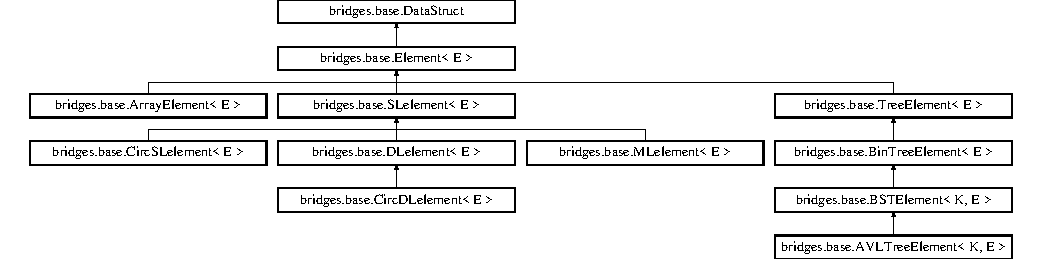
\includegraphics[height=4.647303cm]{classbridges_1_1base_1_1_element}
\end{center}
\end{figure}
\subsection*{Public Member Functions}
\begin{DoxyCompactItemize}
\item 
\hyperlink{classbridges_1_1base_1_1_element_aa5fc5728f2ed4b041118a77409442390}{Element} ()
\item 
\hyperlink{classbridges_1_1base_1_1_element_a6cb9b3b85b923602aad5c1be6696d825}{Element} (E val)
\item 
\hyperlink{classbridges_1_1base_1_1_element_a14e857e8050eac518900a458f0364d8e}{Element} (String label, E val)
\item 
\hyperlink{classbridges_1_1base_1_1_element_a91db9de70b65a1d7b5f27c1c0b909832}{Element} (\hyperlink{classbridges_1_1base_1_1_element}{Element}$<$ E $>$ original)
\item 
String \hyperlink{classbridges_1_1base_1_1_element_ad5496f568b4cca3909800eceea5fb47d}{get\+Identifier} ()
\item 
\hyperlink{classbridges_1_1base_1_1_element_visualizer}{Element\+Visualizer} \hyperlink{classbridges_1_1base_1_1_element_a42c84d41dfb7bd05a586e303cb33de72}{get\+Visualizer} ()
\item 
void \hyperlink{classbridges_1_1base_1_1_element_a5befa95788099f1bc72cdf5361c55bed}{set\+Visualizer} (\hyperlink{classbridges_1_1base_1_1_element_visualizer}{Element\+Visualizer} visualizer)
\item 
\hyperlink{classbridges_1_1base_1_1_link_visualizer}{Link\+Visualizer} \hyperlink{classbridges_1_1base_1_1_element_a7978552c7b36e28c302f611fc1958e7f}{get\+Link\+Visualizer} (\hyperlink{classbridges_1_1base_1_1_element}{Element}$<$ E $>$ el)
\item 
String \hyperlink{classbridges_1_1base_1_1_element_aa235244426486921bef319a28616bf8b}{get\+Class\+Name} ()
\item 
int \hyperlink{classbridges_1_1base_1_1_element_a6cd4c4f15c6a4f87f59e443cffe87a20}{compare\+To} (\hyperlink{classbridges_1_1base_1_1_element}{Element}$<$ E $>$ e1)
\item 
boolean \hyperlink{classbridges_1_1base_1_1_element_aff10d60700eb1aceca5c0b519bdccccb}{equals} (\hyperlink{classbridges_1_1base_1_1_element}{Element}$<$ E $>$ e1)
\item 
String \hyperlink{classbridges_1_1base_1_1_element_a16c4c7e0d511fbf0e205d5606b9d690e}{get\+Representation} ()
\item 
String \hyperlink{classbridges_1_1base_1_1_element_a5c831a0238de487765f6021a887f1542}{get\+Label} ()
\item 
void \hyperlink{classbridges_1_1base_1_1_element_a942ccd766aeca0c4fdbe27ef8cbe78d9}{set\+Label} (String label)
\item 
String \hyperlink{classbridges_1_1base_1_1_element_acd2191242df8a7bf2e8b6ced87880ba6}{arrange\+Label} (String label, int word\+Number)
\item 
E \hyperlink{classbridges_1_1base_1_1_element_a44ddc61db34b6cf0bab7dfba667d54af}{get\+Value} ()
\item 
void \hyperlink{classbridges_1_1base_1_1_element_ab3cf1241da0bc4c59cea9d6f0fd7aaf4}{set\+Value} (E value)
\item 
String \hyperlink{classbridges_1_1base_1_1_element_a7dc685e317fd9dc2e73e049a9f907e42}{to\+String} ()
\end{DoxyCompactItemize}
\subsection*{Protected Member Functions}
\begin{DoxyCompactItemize}
\item 
String \hyperlink{classbridges_1_1base_1_1_element_a6a1b70fa4b1936d10c6deb433acf8cd9}{get\+Data\+Struct\+Type} ()
\item 
void \hyperlink{classbridges_1_1base_1_1_element_af1a60f4e6a91d379179f7d56e6dc3829}{validate\+Val} (E value)
\end{DoxyCompactItemize}
\subsection*{Additional Inherited Members}


\subsection{Detailed Description}
This is the main superclass in B\+R\+I\+D\+G\+ES for deriving a number of objects used in building arrays, lists, trees and graph data structures. 

\hyperlink{classbridges_1_1base_1_1_d_lelement}{D\+Lelement}, \hyperlink{classbridges_1_1base_1_1_circ_s_lelement}{Circ\+S\+Lelement}, \hyperlink{classbridges_1_1base_1_1_circ_d_lelement}{Circ\+D\+Lelement}, \hyperlink{classbridges_1_1base_1_1_tree_element}{Tree\+Element}, \hyperlink{classbridges_1_1base_1_1_bin_tree_element}{Bin\+Tree\+Element}, \hyperlink{classbridges_1_1base_1_1_b_s_t_element}{B\+S\+T\+Element}, \hyperlink{classbridges_1_1base_1_1_a_v_l_tree_element}{A\+V\+L\+Tree\+Element} are all subclasses. \hyperlink{classbridges_1_1base_1_1_element}{Element} contains visualizer objects (\hyperlink{classbridges_1_1base_1_1_element_visualizer}{Element\+Visualizer}, \hyperlink{classbridges_1_1base_1_1_link_visualizer}{Link\+Visualizer}) for specifying visual attributes. It also contains a label that is used in the visualization.

\begin{DoxyAuthor}{Author}
Mihai Mehedint, Kalpathi Subramanian
\end{DoxyAuthor}

\begin{DoxyParams}{Parameters}
{\em generic} & $<$\+E$>$ \\
\hline
\end{DoxyParams}


\subsection{Constructor \& Destructor Documentation}
\hypertarget{classbridges_1_1base_1_1_element_aa5fc5728f2ed4b041118a77409442390}{}\label{classbridges_1_1base_1_1_element_aa5fc5728f2ed4b041118a77409442390} 
\index{bridges\+::base\+::\+Element@{bridges\+::base\+::\+Element}!Element@{Element}}
\index{Element@{Element}!bridges\+::base\+::\+Element@{bridges\+::base\+::\+Element}}
\subsubsection{\texorpdfstring{Element()}{Element()}\hspace{0.1cm}{\footnotesize\ttfamily [1/4]}}
{\footnotesize\ttfamily \hyperlink{classbridges_1_1base_1_1_element}{bridges.\+base.\+Element}$<$ E $>$.\hyperlink{classbridges_1_1base_1_1_element}{Element} (\begin{DoxyParamCaption}{ }\end{DoxyParamCaption})}

\hyperlink{classbridges_1_1base_1_1_element}{Element} constructor creates an \hyperlink{classbridges_1_1base_1_1_element_visualizer}{Element\+Visualizer} object sets a unique identifier for the current \hyperlink{classbridges_1_1base_1_1_element}{Element} normally used from subclasses \hypertarget{classbridges_1_1base_1_1_element_a6cb9b3b85b923602aad5c1be6696d825}{}\label{classbridges_1_1base_1_1_element_a6cb9b3b85b923602aad5c1be6696d825} 
\index{bridges\+::base\+::\+Element@{bridges\+::base\+::\+Element}!Element@{Element}}
\index{Element@{Element}!bridges\+::base\+::\+Element@{bridges\+::base\+::\+Element}}
\subsubsection{\texorpdfstring{Element()}{Element()}\hspace{0.1cm}{\footnotesize\ttfamily [2/4]}}
{\footnotesize\ttfamily \hyperlink{classbridges_1_1base_1_1_element}{bridges.\+base.\+Element}$<$ E $>$.\hyperlink{classbridges_1_1base_1_1_element}{Element} (\begin{DoxyParamCaption}\item[{E}]{val }\end{DoxyParamCaption})}

the constructor of \hyperlink{classbridges_1_1base_1_1_element}{Element} 
\begin{DoxyParams}{Parameters}
{\em val} & will be used to construct \hyperlink{classbridges_1_1base_1_1_element}{Element} \\
\hline
\end{DoxyParams}
\hypertarget{classbridges_1_1base_1_1_element_a14e857e8050eac518900a458f0364d8e}{}\label{classbridges_1_1base_1_1_element_a14e857e8050eac518900a458f0364d8e} 
\index{bridges\+::base\+::\+Element@{bridges\+::base\+::\+Element}!Element@{Element}}
\index{Element@{Element}!bridges\+::base\+::\+Element@{bridges\+::base\+::\+Element}}
\subsubsection{\texorpdfstring{Element()}{Element()}\hspace{0.1cm}{\footnotesize\ttfamily [3/4]}}
{\footnotesize\ttfamily \hyperlink{classbridges_1_1base_1_1_element}{bridges.\+base.\+Element}$<$ E $>$.\hyperlink{classbridges_1_1base_1_1_element}{Element} (\begin{DoxyParamCaption}\item[{String}]{label,  }\item[{E}]{val }\end{DoxyParamCaption})}

the constructor of \hyperlink{classbridges_1_1base_1_1_element}{Element} 
\begin{DoxyParams}{Parameters}
{\em label} & the string that is visible on the Bridges Visualization \\
\hline
{\em val} & will be used to construct \hyperlink{classbridges_1_1base_1_1_element}{Element} \\
\hline
\end{DoxyParams}
\hypertarget{classbridges_1_1base_1_1_element_a91db9de70b65a1d7b5f27c1c0b909832}{}\label{classbridges_1_1base_1_1_element_a91db9de70b65a1d7b5f27c1c0b909832} 
\index{bridges\+::base\+::\+Element@{bridges\+::base\+::\+Element}!Element@{Element}}
\index{Element@{Element}!bridges\+::base\+::\+Element@{bridges\+::base\+::\+Element}}
\subsubsection{\texorpdfstring{Element()}{Element()}\hspace{0.1cm}{\footnotesize\ttfamily [4/4]}}
{\footnotesize\ttfamily \hyperlink{classbridges_1_1base_1_1_element}{bridges.\+base.\+Element}$<$ E $>$.\hyperlink{classbridges_1_1base_1_1_element}{Element} (\begin{DoxyParamCaption}\item[{\hyperlink{classbridges_1_1base_1_1_element}{Element}$<$ E $>$}]{original }\end{DoxyParamCaption})}

performing deep copy of an element when needed 
\begin{DoxyParams}{Parameters}
{\em original} & the \hyperlink{classbridges_1_1base_1_1_element}{Element} that is to be copied \\
\hline
\end{DoxyParams}


\subsection{Member Function Documentation}
\hypertarget{classbridges_1_1base_1_1_element_acd2191242df8a7bf2e8b6ced87880ba6}{}\label{classbridges_1_1base_1_1_element_acd2191242df8a7bf2e8b6ced87880ba6} 
\index{bridges\+::base\+::\+Element@{bridges\+::base\+::\+Element}!arrange\+Label@{arrange\+Label}}
\index{arrange\+Label@{arrange\+Label}!bridges\+::base\+::\+Element@{bridges\+::base\+::\+Element}}
\subsubsection{\texorpdfstring{arrange\+Label()}{arrangeLabel()}}
{\footnotesize\ttfamily String \hyperlink{classbridges_1_1base_1_1_element}{bridges.\+base.\+Element}$<$ E $>$.arrange\+Label (\begin{DoxyParamCaption}\item[{String}]{label,  }\item[{int}]{word\+Number }\end{DoxyParamCaption})}

This method formats the label string using a predefine pattern (D\+I\+V\+I\+D\+E\+\_\+\+K\+EY) and replaces the pattern with the string characters hold by the I\+N\+S\+E\+R\+T\+\_\+\+S\+T\+R\+I\+NG global variable 
\begin{DoxyParams}{Parameters}
{\em label} & \\
\hline
{\em word\+Number} & in very long strings in the case where the whitespace \textbackslash{}s is chosen as a key the word\+Number can be set to replace the whitespace with a newline character \textbackslash{}n at a given number of words (every second or third word) The default value is 0. In most situations we want to replace all patterns found. for more complex patterns the key must be changed like so \char`\"{}((\+John) (.+?))\char`\"{} returns \char`\"{}\+John first\+Word\+After\+John\char`\"{}\+: John writes, John doe, John eats etc. (\textbackslash{}w) matches any word (\textbackslash{}s) one white space (\textbackslash{}s$\ast$) zero or more white spaces, (\textbackslash{}s+) one or more\\
\hline
\end{DoxyParams}
\begin{DoxyReturn}{Returns}

\end{DoxyReturn}
\hypertarget{classbridges_1_1base_1_1_element_a6cd4c4f15c6a4f87f59e443cffe87a20}{}\label{classbridges_1_1base_1_1_element_a6cd4c4f15c6a4f87f59e443cffe87a20} 
\index{bridges\+::base\+::\+Element@{bridges\+::base\+::\+Element}!compare\+To@{compare\+To}}
\index{compare\+To@{compare\+To}!bridges\+::base\+::\+Element@{bridges\+::base\+::\+Element}}
\subsubsection{\texorpdfstring{compare\+To()}{compareTo()}}
{\footnotesize\ttfamily int \hyperlink{classbridges_1_1base_1_1_element}{bridges.\+base.\+Element}$<$ E $>$.compare\+To (\begin{DoxyParamCaption}\item[{\hyperlink{classbridges_1_1base_1_1_element}{Element}$<$ E $>$}]{e1 }\end{DoxyParamCaption})}

Comparison between 2 elements 
\begin{DoxyParams}{Parameters}
{\em e1} & the \hyperlink{classbridges_1_1base_1_1_element}{Element} to compare this with \\
\hline
\end{DoxyParams}
\begin{DoxyReturn}{Returns}
0 if the 2 elements have the same label and the same identifier and a non\+Zero integer otherwise 
\end{DoxyReturn}
\hypertarget{classbridges_1_1base_1_1_element_aff10d60700eb1aceca5c0b519bdccccb}{}\label{classbridges_1_1base_1_1_element_aff10d60700eb1aceca5c0b519bdccccb} 
\index{bridges\+::base\+::\+Element@{bridges\+::base\+::\+Element}!equals@{equals}}
\index{equals@{equals}!bridges\+::base\+::\+Element@{bridges\+::base\+::\+Element}}
\subsubsection{\texorpdfstring{equals()}{equals()}}
{\footnotesize\ttfamily boolean \hyperlink{classbridges_1_1base_1_1_element}{bridges.\+base.\+Element}$<$ E $>$.equals (\begin{DoxyParamCaption}\item[{\hyperlink{classbridges_1_1base_1_1_element}{Element}$<$ E $>$}]{e1 }\end{DoxyParamCaption})}

This method compares 2 Elements 
\begin{DoxyParams}{Parameters}
{\em e1} & \\
\hline
\end{DoxyParams}
\begin{DoxyReturn}{Returns}
boolean 
\end{DoxyReturn}
\hypertarget{classbridges_1_1base_1_1_element_aa235244426486921bef319a28616bf8b}{}\label{classbridges_1_1base_1_1_element_aa235244426486921bef319a28616bf8b} 
\index{bridges\+::base\+::\+Element@{bridges\+::base\+::\+Element}!get\+Class\+Name@{get\+Class\+Name}}
\index{get\+Class\+Name@{get\+Class\+Name}!bridges\+::base\+::\+Element@{bridges\+::base\+::\+Element}}
\subsubsection{\texorpdfstring{get\+Class\+Name()}{getClassName()}}
{\footnotesize\ttfamily String \hyperlink{classbridges_1_1base_1_1_element}{bridges.\+base.\+Element}$<$ E $>$.get\+Class\+Name (\begin{DoxyParamCaption}{ }\end{DoxyParamCaption})}

This method returns the name of the class \begin{DoxyReturn}{Returns}
the class name \char`\"{}\+Element\char`\"{} 
\end{DoxyReturn}
\hypertarget{classbridges_1_1base_1_1_element_a6a1b70fa4b1936d10c6deb433acf8cd9}{}\label{classbridges_1_1base_1_1_element_a6a1b70fa4b1936d10c6deb433acf8cd9} 
\index{bridges\+::base\+::\+Element@{bridges\+::base\+::\+Element}!get\+Data\+Struct\+Type@{get\+Data\+Struct\+Type}}
\index{get\+Data\+Struct\+Type@{get\+Data\+Struct\+Type}!bridges\+::base\+::\+Element@{bridges\+::base\+::\+Element}}
\subsubsection{\texorpdfstring{get\+Data\+Struct\+Type()}{getDataStructType()}}
{\footnotesize\ttfamily String \hyperlink{classbridges_1_1base_1_1_element}{bridges.\+base.\+Element}$<$ E $>$.get\+Data\+Struct\+Type (\begin{DoxyParamCaption}{ }\end{DoxyParamCaption})\hspace{0.3cm}{\ttfamily [protected]}}

\hypertarget{classbridges_1_1base_1_1_element_ad5496f568b4cca3909800eceea5fb47d}{}\label{classbridges_1_1base_1_1_element_ad5496f568b4cca3909800eceea5fb47d} 
\index{bridges\+::base\+::\+Element@{bridges\+::base\+::\+Element}!get\+Identifier@{get\+Identifier}}
\index{get\+Identifier@{get\+Identifier}!bridges\+::base\+::\+Element@{bridges\+::base\+::\+Element}}
\subsubsection{\texorpdfstring{get\+Identifier()}{getIdentifier()}}
{\footnotesize\ttfamily String \hyperlink{classbridges_1_1base_1_1_element}{bridges.\+base.\+Element}$<$ E $>$.get\+Identifier (\begin{DoxyParamCaption}{ }\end{DoxyParamCaption})}

this method returns the element\textquotesingle{}s unique identifier \begin{DoxyReturn}{Returns}
the string identifier 
\end{DoxyReturn}
\hypertarget{classbridges_1_1base_1_1_element_a5c831a0238de487765f6021a887f1542}{}\label{classbridges_1_1base_1_1_element_a5c831a0238de487765f6021a887f1542} 
\index{bridges\+::base\+::\+Element@{bridges\+::base\+::\+Element}!get\+Label@{get\+Label}}
\index{get\+Label@{get\+Label}!bridges\+::base\+::\+Element@{bridges\+::base\+::\+Element}}
\subsubsection{\texorpdfstring{get\+Label()}{getLabel()}}
{\footnotesize\ttfamily String \hyperlink{classbridges_1_1base_1_1_element}{bridges.\+base.\+Element}$<$ E $>$.get\+Label (\begin{DoxyParamCaption}{ }\end{DoxyParamCaption})}

This method returns the existing value of the label fields \begin{DoxyReturn}{Returns}
the label of the \hyperlink{classbridges_1_1base_1_1_element}{Element} that shows up on the Bridges Visualization 
\end{DoxyReturn}
\hypertarget{classbridges_1_1base_1_1_element_a7978552c7b36e28c302f611fc1958e7f}{}\label{classbridges_1_1base_1_1_element_a7978552c7b36e28c302f611fc1958e7f} 
\index{bridges\+::base\+::\+Element@{bridges\+::base\+::\+Element}!get\+Link\+Visualizer@{get\+Link\+Visualizer}}
\index{get\+Link\+Visualizer@{get\+Link\+Visualizer}!bridges\+::base\+::\+Element@{bridges\+::base\+::\+Element}}
\subsubsection{\texorpdfstring{get\+Link\+Visualizer()}{getLinkVisualizer()}}
{\footnotesize\ttfamily \hyperlink{classbridges_1_1base_1_1_link_visualizer}{Link\+Visualizer} \hyperlink{classbridges_1_1base_1_1_element}{bridges.\+base.\+Element}$<$ E $>$.get\+Link\+Visualizer (\begin{DoxyParamCaption}\item[{\hyperlink{classbridges_1_1base_1_1_element}{Element}$<$ E $>$}]{el }\end{DoxyParamCaption})}

Returns the \hyperlink{classbridges_1_1base_1_1_element}{Element}\textquotesingle{}s link visualizer object that is linked to element el  \hyperlink{classbridges_1_1base_1_1_element}{Element} el -- the element terminating the link \begin{DoxyReturn}{Returns}
the link visualizer 
\end{DoxyReturn}
\hypertarget{classbridges_1_1base_1_1_element_a16c4c7e0d511fbf0e205d5606b9d690e}{}\label{classbridges_1_1base_1_1_element_a16c4c7e0d511fbf0e205d5606b9d690e} 
\index{bridges\+::base\+::\+Element@{bridges\+::base\+::\+Element}!get\+Representation@{get\+Representation}}
\index{get\+Representation@{get\+Representation}!bridges\+::base\+::\+Element@{bridges\+::base\+::\+Element}}
\subsubsection{\texorpdfstring{get\+Representation()}{getRepresentation()}}
{\footnotesize\ttfamily String \hyperlink{classbridges_1_1base_1_1_element}{bridges.\+base.\+Element}$<$ E $>$.get\+Representation (\begin{DoxyParamCaption}{ }\end{DoxyParamCaption})}

Internal code for getting the properties of the \hyperlink{classbridges_1_1base_1_1_element}{Element} object. It produces (without the spaces or newlines)\+: \{ \char`\"{}name\char`\"{}\+: \char`\"{}\+Some label\char`\"{}, \char`\"{}other C\+S\+S properties like color\char`\"{}\+: any\+\_\+\+J\+S\+O\+N\+\_\+value \} \begin{DoxyReturn}{Returns}
the encoded J\+S\+ON string 
\end{DoxyReturn}
\hypertarget{classbridges_1_1base_1_1_element_a44ddc61db34b6cf0bab7dfba667d54af}{}\label{classbridges_1_1base_1_1_element_a44ddc61db34b6cf0bab7dfba667d54af} 
\index{bridges\+::base\+::\+Element@{bridges\+::base\+::\+Element}!get\+Value@{get\+Value}}
\index{get\+Value@{get\+Value}!bridges\+::base\+::\+Element@{bridges\+::base\+::\+Element}}
\subsubsection{\texorpdfstring{get\+Value()}{getValue()}}
{\footnotesize\ttfamily E \hyperlink{classbridges_1_1base_1_1_element}{bridges.\+base.\+Element}$<$ E $>$.get\+Value (\begin{DoxyParamCaption}{ }\end{DoxyParamCaption})}

this method returns the value E for the current \hyperlink{classbridges_1_1base_1_1_element}{Element} \begin{DoxyReturn}{Returns}
the value 
\end{DoxyReturn}
\hypertarget{classbridges_1_1base_1_1_element_a42c84d41dfb7bd05a586e303cb33de72}{}\label{classbridges_1_1base_1_1_element_a42c84d41dfb7bd05a586e303cb33de72} 
\index{bridges\+::base\+::\+Element@{bridges\+::base\+::\+Element}!get\+Visualizer@{get\+Visualizer}}
\index{get\+Visualizer@{get\+Visualizer}!bridges\+::base\+::\+Element@{bridges\+::base\+::\+Element}}
\subsubsection{\texorpdfstring{get\+Visualizer()}{getVisualizer()}}
{\footnotesize\ttfamily \hyperlink{classbridges_1_1base_1_1_element_visualizer}{Element\+Visualizer} \hyperlink{classbridges_1_1base_1_1_element}{bridges.\+base.\+Element}$<$ E $>$.get\+Visualizer (\begin{DoxyParamCaption}{ }\end{DoxyParamCaption})}

Returns the \hyperlink{classbridges_1_1base_1_1_element}{Element}\textquotesingle{}s visualizer object \begin{DoxyReturn}{Returns}
the visualizer 
\end{DoxyReturn}
\hypertarget{classbridges_1_1base_1_1_element_a942ccd766aeca0c4fdbe27ef8cbe78d9}{}\label{classbridges_1_1base_1_1_element_a942ccd766aeca0c4fdbe27ef8cbe78d9} 
\index{bridges\+::base\+::\+Element@{bridges\+::base\+::\+Element}!set\+Label@{set\+Label}}
\index{set\+Label@{set\+Label}!bridges\+::base\+::\+Element@{bridges\+::base\+::\+Element}}
\subsubsection{\texorpdfstring{set\+Label()}{setLabel()}}
{\footnotesize\ttfamily void \hyperlink{classbridges_1_1base_1_1_element}{bridges.\+base.\+Element}$<$ E $>$.set\+Label (\begin{DoxyParamCaption}\item[{String}]{label }\end{DoxyParamCaption})}

This method sets the label 
\begin{DoxyParams}{Parameters}
{\em label} & the label to set \\
\hline
\end{DoxyParams}
\hypertarget{classbridges_1_1base_1_1_element_ab3cf1241da0bc4c59cea9d6f0fd7aaf4}{}\label{classbridges_1_1base_1_1_element_ab3cf1241da0bc4c59cea9d6f0fd7aaf4} 
\index{bridges\+::base\+::\+Element@{bridges\+::base\+::\+Element}!set\+Value@{set\+Value}}
\index{set\+Value@{set\+Value}!bridges\+::base\+::\+Element@{bridges\+::base\+::\+Element}}
\subsubsection{\texorpdfstring{set\+Value()}{setValue()}}
{\footnotesize\ttfamily void \hyperlink{classbridges_1_1base_1_1_element}{bridges.\+base.\+Element}$<$ E $>$.set\+Value (\begin{DoxyParamCaption}\item[{E}]{value }\end{DoxyParamCaption})}

This method sets the value field to the E argument value 
\begin{DoxyParams}{Parameters}
{\em value} & the value to set \\
\hline
\end{DoxyParams}
\hypertarget{classbridges_1_1base_1_1_element_a5befa95788099f1bc72cdf5361c55bed}{}\label{classbridges_1_1base_1_1_element_a5befa95788099f1bc72cdf5361c55bed} 
\index{bridges\+::base\+::\+Element@{bridges\+::base\+::\+Element}!set\+Visualizer@{set\+Visualizer}}
\index{set\+Visualizer@{set\+Visualizer}!bridges\+::base\+::\+Element@{bridges\+::base\+::\+Element}}
\subsubsection{\texorpdfstring{set\+Visualizer()}{setVisualizer()}}
{\footnotesize\ttfamily void \hyperlink{classbridges_1_1base_1_1_element}{bridges.\+base.\+Element}$<$ E $>$.set\+Visualizer (\begin{DoxyParamCaption}\item[{\hyperlink{classbridges_1_1base_1_1_element_visualizer}{Element\+Visualizer}}]{visualizer }\end{DoxyParamCaption})}

This method sets the visualizer object for the current element object 
\begin{DoxyParams}{Parameters}
{\em visualizer} & the visualizer to set \\
\hline
\end{DoxyParams}
\hypertarget{classbridges_1_1base_1_1_element_a7dc685e317fd9dc2e73e049a9f907e42}{}\label{classbridges_1_1base_1_1_element_a7dc685e317fd9dc2e73e049a9f907e42} 
\index{bridges\+::base\+::\+Element@{bridges\+::base\+::\+Element}!to\+String@{to\+String}}
\index{to\+String@{to\+String}!bridges\+::base\+::\+Element@{bridges\+::base\+::\+Element}}
\subsubsection{\texorpdfstring{to\+String()}{toString()}}
{\footnotesize\ttfamily String \hyperlink{classbridges_1_1base_1_1_element}{bridges.\+base.\+Element}$<$ E $>$.to\+String (\begin{DoxyParamCaption}{ }\end{DoxyParamCaption})}

\hypertarget{classbridges_1_1base_1_1_element_af1a60f4e6a91d379179f7d56e6dc3829}{}\label{classbridges_1_1base_1_1_element_af1a60f4e6a91d379179f7d56e6dc3829} 
\index{bridges\+::base\+::\+Element@{bridges\+::base\+::\+Element}!validate\+Val@{validate\+Val}}
\index{validate\+Val@{validate\+Val}!bridges\+::base\+::\+Element@{bridges\+::base\+::\+Element}}
\subsubsection{\texorpdfstring{validate\+Val()}{validateVal()}}
{\footnotesize\ttfamily void \hyperlink{classbridges_1_1base_1_1_element}{bridges.\+base.\+Element}$<$ E $>$.validate\+Val (\begin{DoxyParamCaption}\item[{E}]{value }\end{DoxyParamCaption})\hspace{0.3cm}{\ttfamily [protected]}}

Validates the \hyperlink{classbridges_1_1base_1_1_element}{Element}\textquotesingle{}s value when the \hyperlink{classbridges_1_1base_1_1_element}{Element} is created A non null value is expected this will be unnecessary after we modify the server 
\begin{DoxyParams}{Parameters}
{\em E\+Lement} & value \\
\hline
\end{DoxyParams}


The documentation for this class was generated from the following file\+:\begin{DoxyCompactItemize}
\item 
/\+Users/kalpathi/gr/bridges/client/java/bridges16/src/main/java/edu/uncc/cs/bridges\+\_\+v21/base/\hyperlink{_element_8java}{Element.\+java}\end{DoxyCompactItemize}

\hypertarget{classbridges_1_1base_1_1_element_visualizer}{}\section{bridges.\+base.\+Element\+Visualizer Class Reference}
\label{classbridges_1_1base_1_1_element_visualizer}\index{bridges.\+base.\+Element\+Visualizer@{bridges.\+base.\+Element\+Visualizer}}


This class maintains the visual attributes of each B\+R\+I\+D\+G\+E\+S element.  


\subsection*{Public Member Functions}
\begin{DoxyCompactItemize}
\item 
\hyperlink{classbridges_1_1base_1_1_element_visualizer_acbca874876ec1e8dbbde6484a4fc056e}{Element\+Visualizer} ()
\item 
\hyperlink{classbridges_1_1base_1_1_element_visualizer_a5c0d9fe8051ebc816372b9836689fdfa}{Element\+Visualizer} (String a\+Color)
\item 
\hyperlink{classbridges_1_1base_1_1_element_visualizer_ab62b1b06907fbeddfcee2b4b297e1021}{Element\+Visualizer} (String a\+Color, String a\+Shape)
\item 
\hyperlink{classbridges_1_1base_1_1_element_visualizer_ab32f66b72ccf0a26c03ba44006da9ac6}{Element\+Visualizer} (double size)
\item 
\hyperlink{classbridges_1_1base_1_1_element_visualizer_a9bf06ca1b6c215e079ab33ccd99633e8}{Element\+Visualizer} (String a\+Color, String a\+Shape, float opacity, double size)
\item 
\hyperlink{classbridges_1_1base_1_1_element_visualizer_a5b48cbda94a4e84e40de41fe156e2497}{Element\+Visualizer} (\hyperlink{classbridges_1_1base_1_1_element_visualizer}{Element\+Visualizer} v)
\item 
void \hyperlink{classbridges_1_1base_1_1_element_visualizer_aba410184f7df495594fc1fa7948335a5}{set\+Size} (double sz)
\item 
double \hyperlink{classbridges_1_1base_1_1_element_visualizer_a0b7673bf724e3df1f94df50ad95ca5b1}{get\+Size} ()
\item 
void \hyperlink{classbridges_1_1base_1_1_element_visualizer_ad7ff2a772741301c08943a58ffccca38}{set\+Color} (String col\+\_\+name)  throws Invalid\+Value\+Exception 
\item 
void \hyperlink{classbridges_1_1base_1_1_element_visualizer_a84fad1c8abe43b20c68c1800d7630918}{set\+Color} (Integer r, Integer g, Integer b, float a)
\item 
void \hyperlink{classbridges_1_1base_1_1_element_visualizer_a33172ab908f3b6f9740727b0bfe91565}{set\+Color} (\hyperlink{classbridges_1_1base_1_1_color}{Color} c)
\item 
\hyperlink{classbridges_1_1base_1_1_color}{Color} \hyperlink{classbridges_1_1base_1_1_element_visualizer_a3bf821b9bfa02746882bac934ce4fb8e}{get\+Color} ()
\item 
String \hyperlink{classbridges_1_1base_1_1_element_visualizer_a8ef0825745e49f32b57e4bf6c891b57e}{get\+Shape} ()
\item 
void \hyperlink{classbridges_1_1base_1_1_element_visualizer_ac3bad991904c8ad23e5233b341381d93}{set\+Shape} (String a\+Shape)
\item 
void \hyperlink{classbridges_1_1base_1_1_element_visualizer_a932f62eb1bd0c92da265a7f903dd0790}{set\+Opacity} (float opacity)
\item 
float \hyperlink{classbridges_1_1base_1_1_element_visualizer_ab86ff39f17f8d1766670b18be88b5492}{get\+Opacity} ()
\item 
void \hyperlink{classbridges_1_1base_1_1_element_visualizer_a04f3416447f2042de7cd21ce5b6a0598}{set\+Location} (double x, double y)
\end{DoxyCompactItemize}


\subsection{Detailed Description}
This class maintains the visual attributes of each B\+R\+I\+D\+G\+E\+S element. 

Visual properties include color, shape, opacity, size and location. Objects of this class are stored as part of the \hyperlink{classbridges_1_1base_1_1_element}{Element} class. Generally, a user will manipulate the \hyperlink{classbridges_1_1base_1_1_element_visualizer}{Element\+Visualizer} returned from the \hyperlink{classbridges_1_1base_1_1_element}{Element}\textquotesingle{}s get\+Visualizer() method, and then set attributes using its methods. Supported attributed values are as follows\+:~\newline


{\bfseries Supported Colors (by name)}\+: 

\char`\"{}red\char`\"{}, \char`\"{}green\char`\"{}, \char`\"{}blue\char`\"{},\char`\"{}yellow\char`\"{},\char`\"{}cyan\char`\"{},\char`\"{}magenta\char`\"{}, \char`\"{}white\char`\"{},, \char`\"{}black\char`\"{}, \char`\"{}orange\char`\"{}, \char`\"{}turquoise\char`\"{}, \char`\"{}maroon\char`\"{}, ~\newline
 \char`\"{}aquamarine\char`\"{}, \char`\"{}azure\char`\"{}, \char`\"{}beige\char`\"{}, \char`\"{}brown\char`\"{}, \char`\"{}tan\char`\"{}, \char`\"{}olive\char`\"{}, \char`\"{}chartreuse\char`\"{}, \char`\"{}khaki\char`\"{}, \char`\"{}bisque\char`\"{}, \char`\"{}coral\char`\"{}, ~\newline
 \char`\"{}pink\char`\"{}, \char`\"{}lavender\char`\"{}, \char`\"{}purple\char`\"{}, \char`\"{}gold\char`\"{} 

{\bfseries  \hyperlink{classbridges_1_1base_1_1_color}{Color} by R\+G\+B\+A Specification \+:} Range\+: 0-\/255 for each component 

{\bfseries Supported Shapes\+: }

\char`\"{}circle\char`\"{}, \char`\"{}square\char`\"{}, \char`\"{}diamond\char`\"{}, \char`\"{}cross\char`\"{}, \char`\"{}triangle\char`\"{}, \char`\"{}star\char`\"{}, \char`\"{}wye\char`\"{} 

{\bfseries  Shape Size} \+: Range (0-\/50) 

{\bfseries  Opacity\+: } Range (0.\+0-\/1.\+0) 

\begin{DoxyAuthor}{Author}
Mihai Mehedint, Kalpathi Subramanian
\end{DoxyAuthor}
\begin{DoxyDate}{Date}
6/22/16, 1/7/17, 5/17/17
\end{DoxyDate}
\begin{DoxySeeAlso}{See also}
Example Tutorial at ~\newline
 \href{http://bridgesuncc.github.io/Hello_World_Tutorials/SLL.html}{\tt http\+://bridgesuncc.\+github.\+io/\+Hello\+\_\+\+World\+\_\+\+Tutorials/\+S\+L\+L.\+html} 
\end{DoxySeeAlso}


\subsection{Constructor \& Destructor Documentation}
\hypertarget{classbridges_1_1base_1_1_element_visualizer_acbca874876ec1e8dbbde6484a4fc056e}{}\index{bridges\+::base\+::\+Element\+Visualizer@{bridges\+::base\+::\+Element\+Visualizer}!Element\+Visualizer@{Element\+Visualizer}}
\index{Element\+Visualizer@{Element\+Visualizer}!bridges\+::base\+::\+Element\+Visualizer@{bridges\+::base\+::\+Element\+Visualizer}}
\subsubsection[{Element\+Visualizer()}]{\setlength{\rightskip}{0pt plus 5cm}bridges.\+base.\+Element\+Visualizer.\+Element\+Visualizer (
\begin{DoxyParamCaption}
{}
\end{DoxyParamCaption}
)}\label{classbridges_1_1base_1_1_element_visualizer_acbca874876ec1e8dbbde6484a4fc056e}
Construct an \hyperlink{classbridges_1_1base_1_1_element_visualizer}{Element\+Visualizer} with the default visualization settings.

The default settings are color = green, opacity = 1.\+0, size = 10.\+0, shape = circle. \hypertarget{classbridges_1_1base_1_1_element_visualizer_a5c0d9fe8051ebc816372b9836689fdfa}{}\index{bridges\+::base\+::\+Element\+Visualizer@{bridges\+::base\+::\+Element\+Visualizer}!Element\+Visualizer@{Element\+Visualizer}}
\index{Element\+Visualizer@{Element\+Visualizer}!bridges\+::base\+::\+Element\+Visualizer@{bridges\+::base\+::\+Element\+Visualizer}}
\subsubsection[{Element\+Visualizer(\+String a\+Color)}]{\setlength{\rightskip}{0pt plus 5cm}bridges.\+base.\+Element\+Visualizer.\+Element\+Visualizer (
\begin{DoxyParamCaption}
\item[{String}]{a\+Color}
\end{DoxyParamCaption}
)}\label{classbridges_1_1base_1_1_element_visualizer_a5c0d9fe8051ebc816372b9836689fdfa}
Construct an \hyperlink{classbridges_1_1base_1_1_element_visualizer}{Element\+Visualizer} with its color set to \char`\"{}a\+Color\char`\"{}.


\begin{DoxyParams}{Parameters}
{\em a\+Color} & the string that represents one of the Bridges colors. \\
\hline
\end{DoxyParams}
\hypertarget{classbridges_1_1base_1_1_element_visualizer_ab62b1b06907fbeddfcee2b4b297e1021}{}\index{bridges\+::base\+::\+Element\+Visualizer@{bridges\+::base\+::\+Element\+Visualizer}!Element\+Visualizer@{Element\+Visualizer}}
\index{Element\+Visualizer@{Element\+Visualizer}!bridges\+::base\+::\+Element\+Visualizer@{bridges\+::base\+::\+Element\+Visualizer}}
\subsubsection[{Element\+Visualizer(\+String a\+Color, String a\+Shape)}]{\setlength{\rightskip}{0pt plus 5cm}bridges.\+base.\+Element\+Visualizer.\+Element\+Visualizer (
\begin{DoxyParamCaption}
\item[{String}]{a\+Color, }
\item[{String}]{a\+Shape}
\end{DoxyParamCaption}
)}\label{classbridges_1_1base_1_1_element_visualizer_ab62b1b06907fbeddfcee2b4b297e1021}
Construct an \hyperlink{classbridges_1_1base_1_1_element_visualizer}{Element\+Visualizer} with its color set to \char`\"{}a\+Color\char`\"{} and shape set to \char`\"{}a\+Shape\char`\"{}.


\begin{DoxyParams}{Parameters}
{\em a\+Color} & the string that represents one of the Bridges colors. \\
\hline
{\em a\+Shape} & the string that represents one of the Bridges shapes \\
\hline
\end{DoxyParams}
\hypertarget{classbridges_1_1base_1_1_element_visualizer_ab32f66b72ccf0a26c03ba44006da9ac6}{}\index{bridges\+::base\+::\+Element\+Visualizer@{bridges\+::base\+::\+Element\+Visualizer}!Element\+Visualizer@{Element\+Visualizer}}
\index{Element\+Visualizer@{Element\+Visualizer}!bridges\+::base\+::\+Element\+Visualizer@{bridges\+::base\+::\+Element\+Visualizer}}
\subsubsection[{Element\+Visualizer(double size)}]{\setlength{\rightskip}{0pt plus 5cm}bridges.\+base.\+Element\+Visualizer.\+Element\+Visualizer (
\begin{DoxyParamCaption}
\item[{double}]{size}
\end{DoxyParamCaption}
)}\label{classbridges_1_1base_1_1_element_visualizer_ab32f66b72ccf0a26c03ba44006da9ac6}
Construct an \hyperlink{classbridges_1_1base_1_1_element_visualizer}{Element\+Visualizer} with its size set to \char`\"{}size\char`\"{}.


\begin{DoxyParams}{Parameters}
{\em size} & the value that represents the size in pixels of the Bridges \hyperlink{classbridges_1_1base_1_1_element}{Element} \\
\hline
\end{DoxyParams}
\hypertarget{classbridges_1_1base_1_1_element_visualizer_a9bf06ca1b6c215e079ab33ccd99633e8}{}\index{bridges\+::base\+::\+Element\+Visualizer@{bridges\+::base\+::\+Element\+Visualizer}!Element\+Visualizer@{Element\+Visualizer}}
\index{Element\+Visualizer@{Element\+Visualizer}!bridges\+::base\+::\+Element\+Visualizer@{bridges\+::base\+::\+Element\+Visualizer}}
\subsubsection[{Element\+Visualizer(\+String a\+Color, String a\+Shape, float opacity, double size)}]{\setlength{\rightskip}{0pt plus 5cm}bridges.\+base.\+Element\+Visualizer.\+Element\+Visualizer (
\begin{DoxyParamCaption}
\item[{String}]{a\+Color, }
\item[{String}]{a\+Shape, }
\item[{float}]{opacity, }
\item[{double}]{size}
\end{DoxyParamCaption}
)}\label{classbridges_1_1base_1_1_element_visualizer_a9bf06ca1b6c215e079ab33ccd99633e8}
Construct an \hyperlink{classbridges_1_1base_1_1_element_visualizer}{Element\+Visualizer} with its color set to \char`\"{}a\+Color\char`\"{}, its shape set to \char`\"{}a\+Shape\char`\"{}, its opacity set to \char`\"{}opacity\char`\"{} and size set to \char`\"{}size\char`\"{}.


\begin{DoxyParams}{Parameters}
{\em a\+Color} & the string that represents one of the Bridges colors. \\
\hline
{\em a\+Shape} & the string that represents one of the Bridges shapes \\
\hline
{\em opacity} & a double between 0 and 1 representing how transparent the node should be on the Bridges Visualization. 0 for invisible, 1 for fully visible, 0-\/1 for varying transparency. \\
\hline
{\em size} & the double that represents the size of the \hyperlink{classbridges_1_1base_1_1_element}{Element} on the Bridges Visualization \\
\hline
\end{DoxyParams}
\hypertarget{classbridges_1_1base_1_1_element_visualizer_a5b48cbda94a4e84e40de41fe156e2497}{}\index{bridges\+::base\+::\+Element\+Visualizer@{bridges\+::base\+::\+Element\+Visualizer}!Element\+Visualizer@{Element\+Visualizer}}
\index{Element\+Visualizer@{Element\+Visualizer}!bridges\+::base\+::\+Element\+Visualizer@{bridges\+::base\+::\+Element\+Visualizer}}
\subsubsection[{Element\+Visualizer(\+Element\+Visualizer v)}]{\setlength{\rightskip}{0pt plus 5cm}bridges.\+base.\+Element\+Visualizer.\+Element\+Visualizer (
\begin{DoxyParamCaption}
\item[{{\bf Element\+Visualizer}}]{v}
\end{DoxyParamCaption}
)}\label{classbridges_1_1base_1_1_element_visualizer_a5b48cbda94a4e84e40de41fe156e2497}
Construct a new \hyperlink{classbridges_1_1base_1_1_element_visualizer}{Element\+Visualizer} with the same color, shape, opacity, and size as \char`\"{}v\char`\"{}


\begin{DoxyParams}{Parameters}
{\em v} & the \hyperlink{classbridges_1_1base_1_1_element_visualizer}{Element\+Visualizer} whose settings you want to copy. \\
\hline
\end{DoxyParams}


\subsection{Member Function Documentation}
\hypertarget{classbridges_1_1base_1_1_element_visualizer_a3bf821b9bfa02746882bac934ce4fb8e}{}\index{bridges\+::base\+::\+Element\+Visualizer@{bridges\+::base\+::\+Element\+Visualizer}!get\+Color@{get\+Color}}
\index{get\+Color@{get\+Color}!bridges\+::base\+::\+Element\+Visualizer@{bridges\+::base\+::\+Element\+Visualizer}}
\subsubsection[{get\+Color()}]{\setlength{\rightskip}{0pt plus 5cm}{\bf Color} bridges.\+base.\+Element\+Visualizer.\+get\+Color (
\begin{DoxyParamCaption}
{}
\end{DoxyParamCaption}
)}\label{classbridges_1_1base_1_1_element_visualizer_a3bf821b9bfa02746882bac934ce4fb8e}
Get the color of the \hyperlink{classbridges_1_1base_1_1_element}{Element} in the Bridges Visualization

\begin{DoxyReturn}{Returns}
\hyperlink{classbridges_1_1base_1_1_color}{Color} object representing the color of the \hyperlink{classbridges_1_1base_1_1_element}{Element} as R,G,B,A components, each in the range 0-\/255 
\end{DoxyReturn}
\hypertarget{classbridges_1_1base_1_1_element_visualizer_ab86ff39f17f8d1766670b18be88b5492}{}\index{bridges\+::base\+::\+Element\+Visualizer@{bridges\+::base\+::\+Element\+Visualizer}!get\+Opacity@{get\+Opacity}}
\index{get\+Opacity@{get\+Opacity}!bridges\+::base\+::\+Element\+Visualizer@{bridges\+::base\+::\+Element\+Visualizer}}
\subsubsection[{get\+Opacity()}]{\setlength{\rightskip}{0pt plus 5cm}float bridges.\+base.\+Element\+Visualizer.\+get\+Opacity (
\begin{DoxyParamCaption}
{}
\end{DoxyParamCaption}
)}\label{classbridges_1_1base_1_1_element_visualizer_ab86ff39f17f8d1766670b18be88b5492}
Get the opacity of the \hyperlink{classbridges_1_1base_1_1_element}{Element} in the Bridges Visualization \begin{DoxyReturn}{Returns}
the opacity value 
\end{DoxyReturn}
\hypertarget{classbridges_1_1base_1_1_element_visualizer_a8ef0825745e49f32b57e4bf6c891b57e}{}\index{bridges\+::base\+::\+Element\+Visualizer@{bridges\+::base\+::\+Element\+Visualizer}!get\+Shape@{get\+Shape}}
\index{get\+Shape@{get\+Shape}!bridges\+::base\+::\+Element\+Visualizer@{bridges\+::base\+::\+Element\+Visualizer}}
\subsubsection[{get\+Shape()}]{\setlength{\rightskip}{0pt plus 5cm}String bridges.\+base.\+Element\+Visualizer.\+get\+Shape (
\begin{DoxyParamCaption}
{}
\end{DoxyParamCaption}
)}\label{classbridges_1_1base_1_1_element_visualizer_a8ef0825745e49f32b57e4bf6c891b57e}
Get the shape of the \hyperlink{classbridges_1_1base_1_1_element}{Element} in the Bridges Visualization.

\begin{DoxyReturn}{Returns}
the string that represents the \hyperlink{classbridges_1_1base_1_1_element}{Element}\textquotesingle{}s shape in the Bridges Visualization. 
\end{DoxyReturn}
\hypertarget{classbridges_1_1base_1_1_element_visualizer_a0b7673bf724e3df1f94df50ad95ca5b1}{}\index{bridges\+::base\+::\+Element\+Visualizer@{bridges\+::base\+::\+Element\+Visualizer}!get\+Size@{get\+Size}}
\index{get\+Size@{get\+Size}!bridges\+::base\+::\+Element\+Visualizer@{bridges\+::base\+::\+Element\+Visualizer}}
\subsubsection[{get\+Size()}]{\setlength{\rightskip}{0pt plus 5cm}double bridges.\+base.\+Element\+Visualizer.\+get\+Size (
\begin{DoxyParamCaption}
{}
\end{DoxyParamCaption}
)}\label{classbridges_1_1base_1_1_element_visualizer_a0b7673bf724e3df1f94df50ad95ca5b1}
Get the size of the \hyperlink{classbridges_1_1base_1_1_element}{Element} in the Bridges Visualiation

\begin{DoxyReturn}{Returns}
the size in pixels of the \hyperlink{classbridges_1_1base_1_1_element}{Element} in the Bridges Visualization 
\end{DoxyReturn}
\hypertarget{classbridges_1_1base_1_1_element_visualizer_ad7ff2a772741301c08943a58ffccca38}{}\index{bridges\+::base\+::\+Element\+Visualizer@{bridges\+::base\+::\+Element\+Visualizer}!set\+Color@{set\+Color}}
\index{set\+Color@{set\+Color}!bridges\+::base\+::\+Element\+Visualizer@{bridges\+::base\+::\+Element\+Visualizer}}
\subsubsection[{set\+Color(\+String col\+\_\+name)}]{\setlength{\rightskip}{0pt plus 5cm}void bridges.\+base.\+Element\+Visualizer.\+set\+Color (
\begin{DoxyParamCaption}
\item[{String}]{col\+\_\+name}
\end{DoxyParamCaption}
) throws {\bf Invalid\+Value\+Exception}}\label{classbridges_1_1base_1_1_element_visualizer_ad7ff2a772741301c08943a58ffccca38}
Set the color of the \hyperlink{classbridges_1_1base_1_1_element}{Element} in the Bridges Visualization to \char`\"{}a\+Color\char`\"{}.


\begin{DoxyParams}{Parameters}
{\em col\+\_\+name} & the string reprsenting the color of the \hyperlink{classbridges_1_1base_1_1_element}{Element} in the Bridges Visualization; supported named colors are \char`\"{}red\char`\"{}, \char`\"{}green\char`\"{}, \char`\"{}blue\char`\"{}, \char`\"{}yellow\char`\"{}, \char`\"{}cyan\char`\"{}, \char`\"{}magenta\char`\"{}, \char`\"{}white\char`\"{}, \char`\"{}black\char`\"{}, \char`\"{}orange\char`\"{}, \char`\"{}turquoise\char`\"{}, \char`\"{}maroon\char`\"{}, \char`\"{}aquamarine\char`\"{}, \char`\"{}azure\char`\"{}, \char`\"{}beige\char`\"{}, \char`\"{}brown\char`\"{}, \char`\"{}tan\char`\"{}, \char`\"{}olive\char`\"{}, \char`\"{}chartreuse\char`\"{}, \char`\"{}khaki\char`\"{}, \char`\"{}bisque\char`\"{}, \char`\"{}coral\char`\"{}, \char`\"{}pink\char`\"{}, \char`\"{}lavender\char`\"{}, \char`\"{}purple\char`\"{}, \char`\"{}gold\char`\"{} \\
\hline
\end{DoxyParams}
\hypertarget{classbridges_1_1base_1_1_element_visualizer_a84fad1c8abe43b20c68c1800d7630918}{}\index{bridges\+::base\+::\+Element\+Visualizer@{bridges\+::base\+::\+Element\+Visualizer}!set\+Color@{set\+Color}}
\index{set\+Color@{set\+Color}!bridges\+::base\+::\+Element\+Visualizer@{bridges\+::base\+::\+Element\+Visualizer}}
\subsubsection[{set\+Color(\+Integer r, Integer g, Integer b, float a)}]{\setlength{\rightskip}{0pt plus 5cm}void bridges.\+base.\+Element\+Visualizer.\+set\+Color (
\begin{DoxyParamCaption}
\item[{Integer}]{r, }
\item[{Integer}]{g, }
\item[{Integer}]{b, }
\item[{float}]{a}
\end{DoxyParamCaption}
)}\label{classbridges_1_1base_1_1_element_visualizer_a84fad1c8abe43b20c68c1800d7630918}
Set the color of the \hyperlink{classbridges_1_1base_1_1_element}{Element} in the Bridges Visualization given R\+G\+B\+A components (0-\/255 range)


\begin{DoxyParams}{Parameters}
{\em r,g,b,a} & color components \\
\hline
\end{DoxyParams}
\hypertarget{classbridges_1_1base_1_1_element_visualizer_a33172ab908f3b6f9740727b0bfe91565}{}\index{bridges\+::base\+::\+Element\+Visualizer@{bridges\+::base\+::\+Element\+Visualizer}!set\+Color@{set\+Color}}
\index{set\+Color@{set\+Color}!bridges\+::base\+::\+Element\+Visualizer@{bridges\+::base\+::\+Element\+Visualizer}}
\subsubsection[{set\+Color(\+Color c)}]{\setlength{\rightskip}{0pt plus 5cm}void bridges.\+base.\+Element\+Visualizer.\+set\+Color (
\begin{DoxyParamCaption}
\item[{{\bf Color}}]{c}
\end{DoxyParamCaption}
)}\label{classbridges_1_1base_1_1_element_visualizer_a33172ab908f3b6f9740727b0bfe91565}
Set the color of the \hyperlink{classbridges_1_1base_1_1_element}{Element} in the Bridges Visualization to \char`\"{}a\+Color\char`\"{}. given a \hyperlink{classbridges_1_1base_1_1_color}{Color} object


\begin{DoxyParams}{Parameters}
{\em col} & \hyperlink{classbridges_1_1base_1_1_color}{Color} object \\
\hline
\end{DoxyParams}
\hypertarget{classbridges_1_1base_1_1_element_visualizer_a04f3416447f2042de7cd21ce5b6a0598}{}\index{bridges\+::base\+::\+Element\+Visualizer@{bridges\+::base\+::\+Element\+Visualizer}!set\+Location@{set\+Location}}
\index{set\+Location@{set\+Location}!bridges\+::base\+::\+Element\+Visualizer@{bridges\+::base\+::\+Element\+Visualizer}}
\subsubsection[{set\+Location(double x, double y)}]{\setlength{\rightskip}{0pt plus 5cm}void bridges.\+base.\+Element\+Visualizer.\+set\+Location (
\begin{DoxyParamCaption}
\item[{double}]{x, }
\item[{double}]{y}
\end{DoxyParamCaption}
)}\label{classbridges_1_1base_1_1_element_visualizer_a04f3416447f2042de7cd21ce5b6a0598}
Set the location (x, y) of the element -\/ used for displaying elements in maps


\begin{DoxyParams}{Parameters}
{\em location} & the X,Y location(array of 2 doubles) to be set \\
\hline
\end{DoxyParams}
\hypertarget{classbridges_1_1base_1_1_element_visualizer_a932f62eb1bd0c92da265a7f903dd0790}{}\index{bridges\+::base\+::\+Element\+Visualizer@{bridges\+::base\+::\+Element\+Visualizer}!set\+Opacity@{set\+Opacity}}
\index{set\+Opacity@{set\+Opacity}!bridges\+::base\+::\+Element\+Visualizer@{bridges\+::base\+::\+Element\+Visualizer}}
\subsubsection[{set\+Opacity(float opacity)}]{\setlength{\rightskip}{0pt plus 5cm}void bridges.\+base.\+Element\+Visualizer.\+set\+Opacity (
\begin{DoxyParamCaption}
\item[{float}]{opacity}
\end{DoxyParamCaption}
)}\label{classbridges_1_1base_1_1_element_visualizer_a932f62eb1bd0c92da265a7f903dd0790}
Sets the opacity of the \hyperlink{classbridges_1_1base_1_1_element}{Element} in the Bridges Visualization


\begin{DoxyParams}{Parameters}
{\em opacity} & a double between 0 and 1 representing how transparent the node should be on the Bridges Visualization. 0 for invisible, 1 for fully visible, a decimal between 0 and 1 for varying transparency. \\
\hline
\end{DoxyParams}
\hypertarget{classbridges_1_1base_1_1_element_visualizer_ac3bad991904c8ad23e5233b341381d93}{}\index{bridges\+::base\+::\+Element\+Visualizer@{bridges\+::base\+::\+Element\+Visualizer}!set\+Shape@{set\+Shape}}
\index{set\+Shape@{set\+Shape}!bridges\+::base\+::\+Element\+Visualizer@{bridges\+::base\+::\+Element\+Visualizer}}
\subsubsection[{set\+Shape(\+String a\+Shape)}]{\setlength{\rightskip}{0pt plus 5cm}void bridges.\+base.\+Element\+Visualizer.\+set\+Shape (
\begin{DoxyParamCaption}
\item[{String}]{a\+Shape}
\end{DoxyParamCaption}
)}\label{classbridges_1_1base_1_1_element_visualizer_ac3bad991904c8ad23e5233b341381d93}
Sets the shape of the \hyperlink{classbridges_1_1base_1_1_element}{Element} in the Bridges Visualization. Supported shapes include \char`\"{}star\char`\"{}, \char`\"{}circle\char`\"{}, \char`\"{}square\char`\"{}, \char`\"{}diamond\char`\"{}, \char`\"{}cross\char`\"{}, \char`\"{}triangle\char`\"{}, \char`\"{}wye\char`\"{}.


\begin{DoxyParams}{Parameters}
{\em a\+Shape} & the string representing the shape of the \hyperlink{classbridges_1_1base_1_1_element}{Element} in the Bridges Visualization \\
\hline
\end{DoxyParams}
\hypertarget{classbridges_1_1base_1_1_element_visualizer_aba410184f7df495594fc1fa7948335a5}{}\index{bridges\+::base\+::\+Element\+Visualizer@{bridges\+::base\+::\+Element\+Visualizer}!set\+Size@{set\+Size}}
\index{set\+Size@{set\+Size}!bridges\+::base\+::\+Element\+Visualizer@{bridges\+::base\+::\+Element\+Visualizer}}
\subsubsection[{set\+Size(double sz)}]{\setlength{\rightskip}{0pt plus 5cm}void bridges.\+base.\+Element\+Visualizer.\+set\+Size (
\begin{DoxyParamCaption}
\item[{double}]{sz}
\end{DoxyParamCaption}
)}\label{classbridges_1_1base_1_1_element_visualizer_aba410184f7df495594fc1fa7948335a5}
Set the size of the \hyperlink{classbridges_1_1base_1_1_element}{Element} in the Bridge Visualization (in pixel units)


\begin{DoxyParams}{Parameters}
{\em size} & the pixel size of the \hyperlink{classbridges_1_1base_1_1_element}{Element} in the Bridges Visualization \\
\hline
\end{DoxyParams}


The documentation for this class was generated from the following file\+:\begin{DoxyCompactItemize}
\item 
/\+Users/kalpathi/gr/bridges/bridges17/java/src/main/java/bridges/base/\hyperlink{_element_visualizer_8java}{Element\+Visualizer.\+java}\end{DoxyCompactItemize}

\hypertarget{classbridges_1_1data__src__dependent_1_1_follower}{}\section{bridges.\+data\+\_\+src\+\_\+dependent.\+Follower Class Reference}
\label{classbridges_1_1data__src__dependent_1_1_follower}\index{bridges.\+data\+\_\+src\+\_\+dependent.\+Follower@{bridges.\+data\+\_\+src\+\_\+dependent.\+Follower}}


Inherits bridges.\+data\+\_\+src\+\_\+dependent.\+Data\+Source.

\subsection*{Public Member Functions}
\begin{DoxyCompactItemize}
\item 
\hyperlink{classbridges_1_1data__src__dependent_1_1_follower_a1da0079bcd425de9e19d18cd69b98240}{Follower} (String a\+Follower)
\item 
String \hyperlink{classbridges_1_1data__src__dependent_1_1_follower_a38620293ea907fbb2b2fca65a72f953f}{get\+Name} ()
\item 
void \hyperlink{classbridges_1_1data__src__dependent_1_1_follower_a3568ebd0132d28f285448b3ce0468199}{set\+Name} (String name)
\item 
String \hyperlink{classbridges_1_1data__src__dependent_1_1_follower_ac01fd01fb2bbbe4eaac327bca9d6a368}{to\+String} ()
\item 
int \hyperlink{classbridges_1_1data__src__dependent_1_1_follower_a36f11800d7769ef93875e00afa984e19}{hash\+Code} ()
\item 
boolean \hyperlink{classbridges_1_1data__src__dependent_1_1_follower_af98127e42a1adb6a64aae684544e571b}{equals} (Object obj)
\end{DoxyCompactItemize}


\subsection{Constructor \& Destructor Documentation}
\hypertarget{classbridges_1_1data__src__dependent_1_1_follower_a1da0079bcd425de9e19d18cd69b98240}{}\index{bridges\+::data\+\_\+src\+\_\+dependent\+::\+Follower@{bridges\+::data\+\_\+src\+\_\+dependent\+::\+Follower}!Follower@{Follower}}
\index{Follower@{Follower}!bridges\+::data\+\_\+src\+\_\+dependent\+::\+Follower@{bridges\+::data\+\_\+src\+\_\+dependent\+::\+Follower}}
\subsubsection[{Follower(\+String a\+Follower)}]{\setlength{\rightskip}{0pt plus 5cm}bridges.\+data\+\_\+src\+\_\+dependent.\+Follower.\+Follower (
\begin{DoxyParamCaption}
\item[{String}]{a\+Follower}
\end{DoxyParamCaption}
)}\label{classbridges_1_1data__src__dependent_1_1_follower_a1da0079bcd425de9e19d18cd69b98240}


\subsection{Member Function Documentation}
\hypertarget{classbridges_1_1data__src__dependent_1_1_follower_af98127e42a1adb6a64aae684544e571b}{}\index{bridges\+::data\+\_\+src\+\_\+dependent\+::\+Follower@{bridges\+::data\+\_\+src\+\_\+dependent\+::\+Follower}!equals@{equals}}
\index{equals@{equals}!bridges\+::data\+\_\+src\+\_\+dependent\+::\+Follower@{bridges\+::data\+\_\+src\+\_\+dependent\+::\+Follower}}
\subsubsection[{equals(\+Object obj)}]{\setlength{\rightskip}{0pt plus 5cm}boolean bridges.\+data\+\_\+src\+\_\+dependent.\+Follower.\+equals (
\begin{DoxyParamCaption}
\item[{Object}]{obj}
\end{DoxyParamCaption}
)}\label{classbridges_1_1data__src__dependent_1_1_follower_af98127e42a1adb6a64aae684544e571b}
\hypertarget{classbridges_1_1data__src__dependent_1_1_follower_a38620293ea907fbb2b2fca65a72f953f}{}\index{bridges\+::data\+\_\+src\+\_\+dependent\+::\+Follower@{bridges\+::data\+\_\+src\+\_\+dependent\+::\+Follower}!get\+Name@{get\+Name}}
\index{get\+Name@{get\+Name}!bridges\+::data\+\_\+src\+\_\+dependent\+::\+Follower@{bridges\+::data\+\_\+src\+\_\+dependent\+::\+Follower}}
\subsubsection[{get\+Name()}]{\setlength{\rightskip}{0pt plus 5cm}String bridges.\+data\+\_\+src\+\_\+dependent.\+Follower.\+get\+Name (
\begin{DoxyParamCaption}
{}
\end{DoxyParamCaption}
)}\label{classbridges_1_1data__src__dependent_1_1_follower_a38620293ea907fbb2b2fca65a72f953f}
This method returns the string name \hypertarget{classbridges_1_1data__src__dependent_1_1_follower_a36f11800d7769ef93875e00afa984e19}{}\index{bridges\+::data\+\_\+src\+\_\+dependent\+::\+Follower@{bridges\+::data\+\_\+src\+\_\+dependent\+::\+Follower}!hash\+Code@{hash\+Code}}
\index{hash\+Code@{hash\+Code}!bridges\+::data\+\_\+src\+\_\+dependent\+::\+Follower@{bridges\+::data\+\_\+src\+\_\+dependent\+::\+Follower}}
\subsubsection[{hash\+Code()}]{\setlength{\rightskip}{0pt plus 5cm}int bridges.\+data\+\_\+src\+\_\+dependent.\+Follower.\+hash\+Code (
\begin{DoxyParamCaption}
{}
\end{DoxyParamCaption}
)}\label{classbridges_1_1data__src__dependent_1_1_follower_a36f11800d7769ef93875e00afa984e19}
\hypertarget{classbridges_1_1data__src__dependent_1_1_follower_a3568ebd0132d28f285448b3ce0468199}{}\index{bridges\+::data\+\_\+src\+\_\+dependent\+::\+Follower@{bridges\+::data\+\_\+src\+\_\+dependent\+::\+Follower}!set\+Name@{set\+Name}}
\index{set\+Name@{set\+Name}!bridges\+::data\+\_\+src\+\_\+dependent\+::\+Follower@{bridges\+::data\+\_\+src\+\_\+dependent\+::\+Follower}}
\subsubsection[{set\+Name(\+String name)}]{\setlength{\rightskip}{0pt plus 5cm}void bridges.\+data\+\_\+src\+\_\+dependent.\+Follower.\+set\+Name (
\begin{DoxyParamCaption}
\item[{String}]{name}
\end{DoxyParamCaption}
)}\label{classbridges_1_1data__src__dependent_1_1_follower_a3568ebd0132d28f285448b3ce0468199}
This method sets the string name \hypertarget{classbridges_1_1data__src__dependent_1_1_follower_ac01fd01fb2bbbe4eaac327bca9d6a368}{}\index{bridges\+::data\+\_\+src\+\_\+dependent\+::\+Follower@{bridges\+::data\+\_\+src\+\_\+dependent\+::\+Follower}!to\+String@{to\+String}}
\index{to\+String@{to\+String}!bridges\+::data\+\_\+src\+\_\+dependent\+::\+Follower@{bridges\+::data\+\_\+src\+\_\+dependent\+::\+Follower}}
\subsubsection[{to\+String()}]{\setlength{\rightskip}{0pt plus 5cm}String bridges.\+data\+\_\+src\+\_\+dependent.\+Follower.\+to\+String (
\begin{DoxyParamCaption}
{}
\end{DoxyParamCaption}
)}\label{classbridges_1_1data__src__dependent_1_1_follower_ac01fd01fb2bbbe4eaac327bca9d6a368}
This method returns the string value 

The documentation for this class was generated from the following file\+:\begin{DoxyCompactItemize}
\item 
/\+Users/krs/gr/bridges/client/java/src/main/java/bridges/data\+\_\+src\+\_\+dependent/\hyperlink{_follower_8java}{Follower.\+java}\end{DoxyCompactItemize}

\hypertarget{classbridges_1_1data__src__dependent_1_1_game}{}\section{bridges.\+data\+\_\+src\+\_\+dependent.\+Game Class Reference}
\label{classbridges_1_1data__src__dependent_1_1_game}\index{bridges.data\_src\_dependent.Game@{bridges.data\_src\_dependent.Game}}


A \mbox{\hyperlink{classbridges_1_1data__src__dependent_1_1_game}{Game}} object, used along with the Games data source.  




Inherits bridges.\+data\+\_\+src\+\_\+dependent.\+Data\+Source.

\subsection*{Public Member Functions}
\begin{DoxyCompactItemize}
\item 
\mbox{\hyperlink{classbridges_1_1data__src__dependent_1_1_game_a9f145dbcbbfbb0432a2cd8631e57173b}{Game}} ()
\item 
\mbox{\hyperlink{classbridges_1_1data__src__dependent_1_1_game_a2bb9d9f659184be2cc9fc68e38433492}{Game}} (String title, String platform, double rating, Vector$<$ String $>$ genre)
\item 
String \mbox{\hyperlink{classbridges_1_1data__src__dependent_1_1_game_af92a6fdd0e852e6cc5d97fb193be4ca9}{get\+Title}} ()
\item 
void \mbox{\hyperlink{classbridges_1_1data__src__dependent_1_1_game_a0c87151b75bc10357aa6829ebfc0cae3}{set\+Title}} (String title)
\item 
String \mbox{\hyperlink{classbridges_1_1data__src__dependent_1_1_game_a1eef8e419c6302ba83ea595491412494}{get\+Platform\+Type}} ()
\item 
void \mbox{\hyperlink{classbridges_1_1data__src__dependent_1_1_game_ab4d51e07186a9228c50210cf661304c7}{set\+Platform\+Type}} (String platform)
\item 
double \mbox{\hyperlink{classbridges_1_1data__src__dependent_1_1_game_a83b444e2c487701b4e9789a6a35ae210}{get\+Rating}} ()
\item 
void \mbox{\hyperlink{classbridges_1_1data__src__dependent_1_1_game_ab59c6ea5ee2721dcca2246e8e287154f}{set\+Rating}} (double rating)
\item 
Vector$<$ String $>$ \mbox{\hyperlink{classbridges_1_1data__src__dependent_1_1_game_ab3c0e46513e71b56a2970ac014b1bf79}{get\+Genre}} ()
\item 
void \mbox{\hyperlink{classbridges_1_1data__src__dependent_1_1_game_ab3c9d9cd9f0acdd7bdc6ea7e1b140868}{set\+Genre}} (Vector$<$ String $>$ genre)
\end{DoxyCompactItemize}


\subsection{Detailed Description}
A \mbox{\hyperlink{classbridges_1_1data__src__dependent_1_1_game}{Game}} object, used along with the Games data source. 

This is a convenience class provided for users who wish to use this data source as part of their application. It provides an A\+PI that makes it easy to access the attributes of this data set.

Refer to tutorial examples to using this data source in data structure assignments.

Refer to tutorial examples to using this data source in data structure assignments.

\begin{DoxyAuthor}{Author}
Kalpathi Subramanian 
\end{DoxyAuthor}
\begin{DoxyDate}{Date}
2/1/17 
\end{DoxyDate}


\subsection{Constructor \& Destructor Documentation}
\mbox{\Hypertarget{classbridges_1_1data__src__dependent_1_1_game_a9f145dbcbbfbb0432a2cd8631e57173b}\label{classbridges_1_1data__src__dependent_1_1_game_a9f145dbcbbfbb0432a2cd8631e57173b}} 
\index{bridges.data\_src\_dependent.Game@{bridges.data\_src\_dependent.Game}!Game@{Game}}
\index{Game@{Game}!bridges.data\_src\_dependent.Game@{bridges.data\_src\_dependent.Game}}
\subsubsection{\texorpdfstring{Game()}{Game()}\hspace{0.1cm}{\footnotesize\ttfamily [1/2]}}
{\footnotesize\ttfamily bridges.\+data\+\_\+src\+\_\+dependent.\+Game.\+Game (\begin{DoxyParamCaption}{ }\end{DoxyParamCaption})}

\mbox{\Hypertarget{classbridges_1_1data__src__dependent_1_1_game_a2bb9d9f659184be2cc9fc68e38433492}\label{classbridges_1_1data__src__dependent_1_1_game_a2bb9d9f659184be2cc9fc68e38433492}} 
\index{bridges.data\_src\_dependent.Game@{bridges.data\_src\_dependent.Game}!Game@{Game}}
\index{Game@{Game}!bridges.data\_src\_dependent.Game@{bridges.data\_src\_dependent.Game}}
\subsubsection{\texorpdfstring{Game()}{Game()}\hspace{0.1cm}{\footnotesize\ttfamily [2/2]}}
{\footnotesize\ttfamily bridges.\+data\+\_\+src\+\_\+dependent.\+Game.\+Game (\begin{DoxyParamCaption}\item[{String}]{title,  }\item[{String}]{platform,  }\item[{double}]{rating,  }\item[{Vector$<$ String $>$}]{genre }\end{DoxyParamCaption})}



\subsection{Member Function Documentation}
\mbox{\Hypertarget{classbridges_1_1data__src__dependent_1_1_game_ab3c0e46513e71b56a2970ac014b1bf79}\label{classbridges_1_1data__src__dependent_1_1_game_ab3c0e46513e71b56a2970ac014b1bf79}} 
\index{bridges.data\_src\_dependent.Game@{bridges.data\_src\_dependent.Game}!getGenre@{getGenre}}
\index{getGenre@{getGenre}!bridges.data\_src\_dependent.Game@{bridges.data\_src\_dependent.Game}}
\subsubsection{\texorpdfstring{getGenre()}{getGenre()}}
{\footnotesize\ttfamily Vector$<$String$>$ bridges.\+data\+\_\+src\+\_\+dependent.\+Game.\+get\+Genre (\begin{DoxyParamCaption}{ }\end{DoxyParamCaption})}

\mbox{\Hypertarget{classbridges_1_1data__src__dependent_1_1_game_a1eef8e419c6302ba83ea595491412494}\label{classbridges_1_1data__src__dependent_1_1_game_a1eef8e419c6302ba83ea595491412494}} 
\index{bridges.data\_src\_dependent.Game@{bridges.data\_src\_dependent.Game}!getPlatformType@{getPlatformType}}
\index{getPlatformType@{getPlatformType}!bridges.data\_src\_dependent.Game@{bridges.data\_src\_dependent.Game}}
\subsubsection{\texorpdfstring{getPlatformType()}{getPlatformType()}}
{\footnotesize\ttfamily String bridges.\+data\+\_\+src\+\_\+dependent.\+Game.\+get\+Platform\+Type (\begin{DoxyParamCaption}{ }\end{DoxyParamCaption})}

\mbox{\Hypertarget{classbridges_1_1data__src__dependent_1_1_game_a83b444e2c487701b4e9789a6a35ae210}\label{classbridges_1_1data__src__dependent_1_1_game_a83b444e2c487701b4e9789a6a35ae210}} 
\index{bridges.data\_src\_dependent.Game@{bridges.data\_src\_dependent.Game}!getRating@{getRating}}
\index{getRating@{getRating}!bridges.data\_src\_dependent.Game@{bridges.data\_src\_dependent.Game}}
\subsubsection{\texorpdfstring{getRating()}{getRating()}}
{\footnotesize\ttfamily double bridges.\+data\+\_\+src\+\_\+dependent.\+Game.\+get\+Rating (\begin{DoxyParamCaption}{ }\end{DoxyParamCaption})}

\mbox{\Hypertarget{classbridges_1_1data__src__dependent_1_1_game_af92a6fdd0e852e6cc5d97fb193be4ca9}\label{classbridges_1_1data__src__dependent_1_1_game_af92a6fdd0e852e6cc5d97fb193be4ca9}} 
\index{bridges.data\_src\_dependent.Game@{bridges.data\_src\_dependent.Game}!getTitle@{getTitle}}
\index{getTitle@{getTitle}!bridges.data\_src\_dependent.Game@{bridges.data\_src\_dependent.Game}}
\subsubsection{\texorpdfstring{getTitle()}{getTitle()}}
{\footnotesize\ttfamily String bridges.\+data\+\_\+src\+\_\+dependent.\+Game.\+get\+Title (\begin{DoxyParamCaption}{ }\end{DoxyParamCaption})}

\mbox{\Hypertarget{classbridges_1_1data__src__dependent_1_1_game_ab3c9d9cd9f0acdd7bdc6ea7e1b140868}\label{classbridges_1_1data__src__dependent_1_1_game_ab3c9d9cd9f0acdd7bdc6ea7e1b140868}} 
\index{bridges.data\_src\_dependent.Game@{bridges.data\_src\_dependent.Game}!setGenre@{setGenre}}
\index{setGenre@{setGenre}!bridges.data\_src\_dependent.Game@{bridges.data\_src\_dependent.Game}}
\subsubsection{\texorpdfstring{setGenre()}{setGenre()}}
{\footnotesize\ttfamily void bridges.\+data\+\_\+src\+\_\+dependent.\+Game.\+set\+Genre (\begin{DoxyParamCaption}\item[{Vector$<$ String $>$}]{genre }\end{DoxyParamCaption})}

\mbox{\Hypertarget{classbridges_1_1data__src__dependent_1_1_game_ab4d51e07186a9228c50210cf661304c7}\label{classbridges_1_1data__src__dependent_1_1_game_ab4d51e07186a9228c50210cf661304c7}} 
\index{bridges.data\_src\_dependent.Game@{bridges.data\_src\_dependent.Game}!setPlatformType@{setPlatformType}}
\index{setPlatformType@{setPlatformType}!bridges.data\_src\_dependent.Game@{bridges.data\_src\_dependent.Game}}
\subsubsection{\texorpdfstring{setPlatformType()}{setPlatformType()}}
{\footnotesize\ttfamily void bridges.\+data\+\_\+src\+\_\+dependent.\+Game.\+set\+Platform\+Type (\begin{DoxyParamCaption}\item[{String}]{platform }\end{DoxyParamCaption})}

\mbox{\Hypertarget{classbridges_1_1data__src__dependent_1_1_game_ab59c6ea5ee2721dcca2246e8e287154f}\label{classbridges_1_1data__src__dependent_1_1_game_ab59c6ea5ee2721dcca2246e8e287154f}} 
\index{bridges.data\_src\_dependent.Game@{bridges.data\_src\_dependent.Game}!setRating@{setRating}}
\index{setRating@{setRating}!bridges.data\_src\_dependent.Game@{bridges.data\_src\_dependent.Game}}
\subsubsection{\texorpdfstring{setRating()}{setRating()}}
{\footnotesize\ttfamily void bridges.\+data\+\_\+src\+\_\+dependent.\+Game.\+set\+Rating (\begin{DoxyParamCaption}\item[{double}]{rating }\end{DoxyParamCaption})}

\mbox{\Hypertarget{classbridges_1_1data__src__dependent_1_1_game_a0c87151b75bc10357aa6829ebfc0cae3}\label{classbridges_1_1data__src__dependent_1_1_game_a0c87151b75bc10357aa6829ebfc0cae3}} 
\index{bridges.data\_src\_dependent.Game@{bridges.data\_src\_dependent.Game}!setTitle@{setTitle}}
\index{setTitle@{setTitle}!bridges.data\_src\_dependent.Game@{bridges.data\_src\_dependent.Game}}
\subsubsection{\texorpdfstring{setTitle()}{setTitle()}}
{\footnotesize\ttfamily void bridges.\+data\+\_\+src\+\_\+dependent.\+Game.\+set\+Title (\begin{DoxyParamCaption}\item[{String}]{title }\end{DoxyParamCaption})}



The documentation for this class was generated from the following file\+:\begin{DoxyCompactItemize}
\item 
/\+Users/kalpathi/gr/bridges/java/src/main/java/bridges/data\+\_\+src\+\_\+dependent/\mbox{\hyperlink{_game_8java}{Game.\+java}}\end{DoxyCompactItemize}

\hypertarget{classbridges_1_1data__src__dependent_1_1_usgs_foo_1_1_geometry}{}\section{bridges.\+data\+\_\+src\+\_\+dependent.\+Usgs\+Foo.\+Geometry Class Reference}
\label{classbridges_1_1data__src__dependent_1_1_usgs_foo_1_1_geometry}\index{bridges.\+data\+\_\+src\+\_\+dependent.\+Usgs\+Foo.\+Geometry@{bridges.\+data\+\_\+src\+\_\+dependent.\+Usgs\+Foo.\+Geometry}}
\subsection*{Classes}
\begin{DoxyCompactItemize}
\item 
class \mbox{\hyperlink{classbridges_1_1data__src__dependent_1_1_usgs_foo_1_1_geometry_1_1_coordinates}{Coordinates}}
\end{DoxyCompactItemize}
\subsection*{Public Attributes}
\begin{DoxyCompactItemize}
\item 
String \mbox{\hyperlink{classbridges_1_1data__src__dependent_1_1_usgs_foo_1_1_geometry_a985b3a46dad2fcd4e798d2f51198bcfd}{type}}
\item 
\mbox{\hyperlink{classbridges_1_1data__src__dependent_1_1_usgs_foo_1_1_geometry_1_1_coordinates}{Coordinates}} \mbox{\hyperlink{classbridges_1_1data__src__dependent_1_1_usgs_foo_1_1_geometry_a339e388c47a5d03c946c875d690ee514}{coordinates}}
\end{DoxyCompactItemize}


\subsection{Member Data Documentation}
\mbox{\Hypertarget{classbridges_1_1data__src__dependent_1_1_usgs_foo_1_1_geometry_a339e388c47a5d03c946c875d690ee514}\label{classbridges_1_1data__src__dependent_1_1_usgs_foo_1_1_geometry_a339e388c47a5d03c946c875d690ee514}} 
\index{bridges\+::data\+\_\+src\+\_\+dependent\+::\+Usgs\+Foo\+::\+Geometry@{bridges\+::data\+\_\+src\+\_\+dependent\+::\+Usgs\+Foo\+::\+Geometry}!coordinates@{coordinates}}
\index{coordinates@{coordinates}!bridges\+::data\+\_\+src\+\_\+dependent\+::\+Usgs\+Foo\+::\+Geometry@{bridges\+::data\+\_\+src\+\_\+dependent\+::\+Usgs\+Foo\+::\+Geometry}}
\subsubsection{\texorpdfstring{coordinates}{coordinates}}
{\footnotesize\ttfamily \mbox{\hyperlink{classbridges_1_1data__src__dependent_1_1_usgs_foo_1_1_geometry_1_1_coordinates}{Coordinates}} bridges.\+data\+\_\+src\+\_\+dependent.\+Usgs\+Foo.\+Geometry.\+coordinates}

\mbox{\Hypertarget{classbridges_1_1data__src__dependent_1_1_usgs_foo_1_1_geometry_a985b3a46dad2fcd4e798d2f51198bcfd}\label{classbridges_1_1data__src__dependent_1_1_usgs_foo_1_1_geometry_a985b3a46dad2fcd4e798d2f51198bcfd}} 
\index{bridges\+::data\+\_\+src\+\_\+dependent\+::\+Usgs\+Foo\+::\+Geometry@{bridges\+::data\+\_\+src\+\_\+dependent\+::\+Usgs\+Foo\+::\+Geometry}!type@{type}}
\index{type@{type}!bridges\+::data\+\_\+src\+\_\+dependent\+::\+Usgs\+Foo\+::\+Geometry@{bridges\+::data\+\_\+src\+\_\+dependent\+::\+Usgs\+Foo\+::\+Geometry}}
\subsubsection{\texorpdfstring{type}{type}}
{\footnotesize\ttfamily String bridges.\+data\+\_\+src\+\_\+dependent.\+Usgs\+Foo.\+Geometry.\+type}



The documentation for this class was generated from the following file\+:\begin{DoxyCompactItemize}
\item 
/\+Users/kalpathi/gr/bridges/client/java/bridges-\/17/src/main/java/edu/uncc/cs/bridges\+\_\+v21/data\+\_\+src\+\_\+dependent/\mbox{\hyperlink{_usgs_foo_8java}{Usgs\+Foo.\+java}}\end{DoxyCompactItemize}

\hypertarget{classbridges_1_1base_1_1_graph_adj_list}{}\section{bridges.\+base.\+Graph\+Adj\+List$<$ K, E1, E2 $>$ Class Template Reference}
\label{classbridges_1_1base_1_1_graph_adj_list}\index{bridges.\+base.\+Graph\+Adj\+List$<$ K, E1, E2 $>$@{bridges.\+base.\+Graph\+Adj\+List$<$ K, E1, E2 $>$}}
Inheritance diagram for bridges.\+base.\+Graph\+Adj\+List$<$ K, E1, E2 $>$\+:\begin{figure}[H]
\begin{center}
\leavevmode
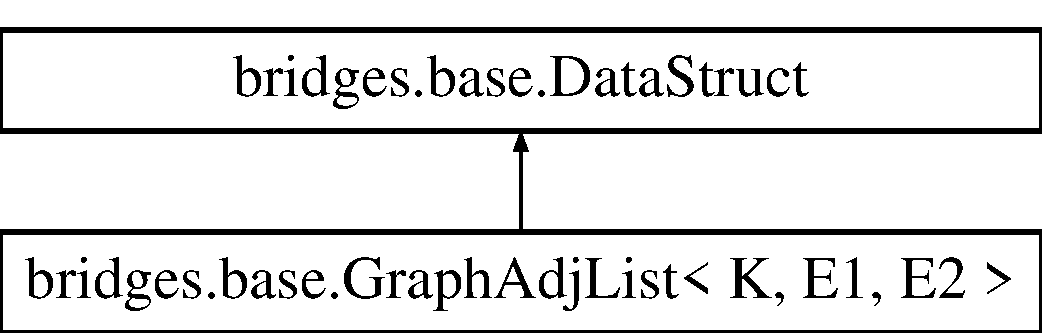
\includegraphics[height=2.000000cm]{classbridges_1_1base_1_1_graph_adj_list}
\end{center}
\end{figure}


\subsection{Detailed Description}
The \hyperlink{classbridges_1_1base_1_1_graph_adj_list}{Graph\+Adj\+List} class can be used to represent adjacency list based graphs in B\+R\+I\+D\+G\+ES. 

The \hyperlink{classbridges_1_1base_1_1_graph_adj_list}{Graph\+Adj\+List} class can be used to represent adjacency list based graphs in B\+R\+I\+D\+G\+ES; it takes 3 generic parameters\+: (1) K, which is an orderable key value used in accessing vertices (in constant time) using a hashmap. This permits data sets that need to be accessed by keys that are strings, (2) E1, for maintaining vertex specific data, and (3) E2, for maintaining edge specific data. The class is a wrapper around the Java Hashmap class and, thus, derives all its operations from it. B\+R\+I\+D\+G\+ES provides methods to visualize the graph and its contents.

The vertices of the graph are held in a Java hashmap, for near constant time access; this enables to use strings or integer ids for vertices. The adjacency lists, also a Java hashmap are built for each vertex and contain the edge (source, destination vertices) in the \hyperlink{classbridges_1_1base_1_1_edge}{Edge} structure, defined separately.

Convenience method \hyperlink{classbridges_1_1base_1_1_graph_adj_list_aca59a3c40af4ae82716ebbfa1751f267}{add\+Vertex()} is provided to add vertices to the graph, and \hyperlink{classbridges_1_1base_1_1_graph_adj_list_a43041976184920e1db1dbe3ad696c6cd}{add\+Edge()} is provided to add edges. Edges are retrieved by using the dual hashmap, given the vertex ids of the edge. Vertices can be styled directly from the vertex element returned by \hyperlink{classbridges_1_1base_1_1_graph_adj_list_aa19cd300a85b05352bdf58720310a112}{get\+Vertex()}, and edges are styled from a \hyperlink{classbridges_1_1base_1_1_link_visualizer}{Link\+Visualizer} one can access through \hyperlink{classbridges_1_1base_1_1_graph_adj_list_af93888dbd2a768a2401619ad5dc95560}{get\+Link\+Visualizer()}. Here is a simple example\+:


\begin{DoxyCode}
GraphAdjList<string, Integer, Double> graph = \textcolor{keyword}{new} GraphAdjList<String, Integer, Double> ();
graph.addVertex(\textcolor{stringliteral}{"a"});
graph.addVertex(\textcolor{stringliteral}{"b"});
graph.addEdge(\textcolor{stringliteral}{"a"}, \textcolor{stringliteral}{"b"});
graph.getVertex(\textcolor{stringliteral}{"a"}).setShape(\textcolor{stringliteral}{"square"});
graph.getLinkVisualizer(\textcolor{stringliteral}{"a"}, \textcolor{stringliteral}{"b"}).setColor(\textcolor{stringliteral}{"yellow"});
\end{DoxyCode}


Adjacency lists are singly linked lists using the B\+R\+I\+D\+G\+ES \hyperlink{classbridges_1_1base_1_1_s_lelement}{S\+Lelement}. Iterators are provided for easy traversal of the adjacency lists. For instance,


\begin{DoxyCode}
GraphAdjList<string, Integer, Double> graph = something();
\textcolor{keywordflow}{for} (Edge<String, Double> e : graph.outgoingEdgeSetOf(\textcolor{stringliteral}{"a"}))
  System.out.println(\textcolor{stringliteral}{"a -> "}+e.getTo());
\end{DoxyCode}


\begin{DoxySeeAlso}{See also}
Example tutorial at \href{http://bridgesuncc.github.io/tutorials/Graph_AL.html}{\tt http\+://bridgesuncc.\+github.\+io/tutorials/\+Graph\+\_\+\+A\+L.\+html}
\end{DoxySeeAlso}
\begin{DoxyAuthor}{Author}
Kalpathi Subramanian, Erik Saule
\end{DoxyAuthor}
\begin{DoxyDate}{Date}
6/29/15, 5/18/17, 4/24/18, 7/14/19
\end{DoxyDate}

\begin{DoxyParams}{Parameters}
{\em K} & orderable key (string, int, etc) that is used to index into vertex \\
\hline
{\em E1} & holds vertex specific information, defined by application \\
\hline
{\em E2} & holds edge specific information, defined by application \\
\hline
\end{DoxyParams}
\subsection*{Public Member Functions}
\begin{DoxyCompactItemize}
\item 
\hyperlink{classbridges_1_1base_1_1_graph_adj_list_aba7e066f43d361418ae6bdf53a23b1de}{Graph\+Adj\+List} ()
\item 
String \hyperlink{classbridges_1_1base_1_1_graph_adj_list_a40c4a2faf20c9847e8ba0d8024236a4b}{get\+Data\+Struct\+Type} ()
\begin{DoxyCompactList}\small\item\em This method gets the data structure type. \end{DoxyCompactList}\item 
void \hyperlink{classbridges_1_1base_1_1_graph_adj_list_aca59a3c40af4ae82716ebbfa1751f267}{add\+Vertex} (K k, E1 e)
\begin{DoxyCompactList}\small\item\em adds a new vertex to the graph. \end{DoxyCompactList}\item 
void \hyperlink{classbridges_1_1base_1_1_graph_adj_list_a43041976184920e1db1dbe3ad696c6cd}{add\+Edge} (K src, K dest)
\begin{DoxyCompactList}\small\item\em adds a new edge to the graph. \end{DoxyCompactList}\item 
void \hyperlink{classbridges_1_1base_1_1_graph_adj_list_aa9fa3cbb6a90de43ee6f0d59c8dce329}{add\+Edge} (K src, K dest, E2 data)
\begin{DoxyCompactList}\small\item\em adds a new edge to the graph. \end{DoxyCompactList}\item 
void \hyperlink{classbridges_1_1base_1_1_graph_adj_list_aa80bfbbe9c4dd130632db1e1165d635e}{set\+Vertex\+Data} (K src, E1 vertex\+\_\+data)
\begin{DoxyCompactList}\small\item\em Sets data for a graph vertex. \end{DoxyCompactList}\item 
E1 \hyperlink{classbridges_1_1base_1_1_graph_adj_list_a3d5f73795bcd5011c425eaca33383454}{get\+Vertex\+Data} (K src)
\begin{DoxyCompactList}\small\item\em Gets data for an edge. \end{DoxyCompactList}\item 
void \hyperlink{classbridges_1_1base_1_1_graph_adj_list_a48041b13b10d5fb677f48a0debfc268e}{set\+Edge\+Data} (K src, K dest, E2 edge\+\_\+data)
\begin{DoxyCompactList}\small\item\em Sets data for an edge. \end{DoxyCompactList}\item 
E2 \hyperlink{classbridges_1_1base_1_1_graph_adj_list_a13cdc7ed89fb211f47e2b04da0b65561}{get\+Edge\+Data} (K src, K dest)
\begin{DoxyCompactList}\small\item\em Gets data for an edge. \end{DoxyCompactList}\item 
Hash\+Map$<$ K, \hyperlink{classbridges_1_1base_1_1_element}{Element}$<$ E1 $>$ $>$ \hyperlink{classbridges_1_1base_1_1_graph_adj_list_acd53b2393db0936ad5812997f67ee1ee}{get\+Vertices} ()
\begin{DoxyCompactList}\small\item\em This method returns the graph vertices. \end{DoxyCompactList}\item 
\hyperlink{classbridges_1_1base_1_1_element}{Element}$<$ E1 $>$ \hyperlink{classbridges_1_1base_1_1_graph_adj_list_aa19cd300a85b05352bdf58720310a112}{get\+Vertex} (K key)
\begin{DoxyCompactList}\small\item\em returns a vertex from its key \end{DoxyCompactList}\item 
Hash\+Map$<$ K, \hyperlink{classbridges_1_1base_1_1_s_lelement}{S\+Lelement}$<$ \hyperlink{classbridges_1_1base_1_1_edge}{Edge}$<$ K, E2 $>$ $>$ $>$ \hyperlink{classbridges_1_1base_1_1_graph_adj_list_a77771e356aa8bf44525be9ae01603989}{get\+Adjacency\+List} ()
\begin{DoxyCompactList}\small\item\em Gets the graph\textquotesingle{}s adjacency list. \end{DoxyCompactList}\item 
\hyperlink{classbridges_1_1base_1_1_s_lelement}{S\+Lelement}$<$ \hyperlink{classbridges_1_1base_1_1_edge}{Edge}$<$ K, E2 $>$ $>$ \hyperlink{classbridges_1_1base_1_1_graph_adj_list_aa8d25bc56b9a172999f0c62ee7e04b6f}{get\+Adjacency\+List} (K vertex)
\begin{DoxyCompactList}\small\item\em Gets the adjacency list of a vertex. \end{DoxyCompactList}\item 
Iterable$<$ \hyperlink{classbridges_1_1base_1_1_edge}{Edge}$<$ K, E2 $>$ $>$ \hyperlink{classbridges_1_1base_1_1_graph_adj_list_a084693f2f464b8f1d21d5ed2a864bf46}{outgoing\+Edge\+Set\+Of} (K vertex)
\begin{DoxyCompactList}\small\item\em returns an iterable set of outgoing edge of a vertex \end{DoxyCompactList}\item 
\hyperlink{classbridges_1_1base_1_1_link_visualizer}{Link\+Visualizer} \hyperlink{classbridges_1_1base_1_1_graph_adj_list_af93888dbd2a768a2401619ad5dc95560}{get\+Link\+Visualizer} (K src, K dest)
\begin{DoxyCompactList}\small\item\em Access a \hyperlink{classbridges_1_1base_1_1_link_visualizer}{Link\+Visualizer} associated with an edge. \end{DoxyCompactList}\item 
\hyperlink{classbridges_1_1base_1_1_element_visualizer}{Element\+Visualizer} \hyperlink{classbridges_1_1base_1_1_graph_adj_list_aafb45833cd5c13b6ce9bdece3fefde6a}{get\+Visualizer} (K vertex)
\begin{DoxyCompactList}\small\item\em Access the \hyperlink{classbridges_1_1base_1_1_element_visualizer}{Element\+Visualizer} associated with a vertex. \end{DoxyCompactList}\item 
void \hyperlink{classbridges_1_1base_1_1_graph_adj_list_a0e2dff032458bb03cb778b571ddcc9b6}{force\+Large\+Visualization} (boolean f)
\begin{DoxyCompactList}\small\item\em Forces the graph use the large graph visualization. \end{DoxyCompactList}\item 
void \hyperlink{classbridges_1_1base_1_1_graph_adj_list_ae14e51214742db0c4dab26c1d409f4ed}{force\+Small\+Visualization} (boolean f)
\begin{DoxyCompactList}\small\item\em Forces the graph to use the small graph visualization. \end{DoxyCompactList}\item 
String \hyperlink{classbridges_1_1base_1_1_graph_adj_list_a9bba66056cdf24197c41fff455e19a6c}{get\+Data\+Structure\+Representation} ()
\end{DoxyCompactItemize}
\subsection*{Additional Inherited Members}


\subsection{Constructor \& Destructor Documentation}
\mbox{\Hypertarget{classbridges_1_1base_1_1_graph_adj_list_aba7e066f43d361418ae6bdf53a23b1de}\label{classbridges_1_1base_1_1_graph_adj_list_aba7e066f43d361418ae6bdf53a23b1de}} 
\index{bridges\+::base\+::\+Graph\+Adj\+List@{bridges\+::base\+::\+Graph\+Adj\+List}!Graph\+Adj\+List@{Graph\+Adj\+List}}
\index{Graph\+Adj\+List@{Graph\+Adj\+List}!bridges\+::base\+::\+Graph\+Adj\+List@{bridges\+::base\+::\+Graph\+Adj\+List}}
\subsubsection{\texorpdfstring{Graph\+Adj\+List()}{GraphAdjList()}}
{\footnotesize\ttfamily \hyperlink{classbridges_1_1base_1_1_graph_adj_list}{bridges.\+base.\+Graph\+Adj\+List}$<$ K, E1, E2 $>$.\hyperlink{classbridges_1_1base_1_1_graph_adj_list}{Graph\+Adj\+List} (\begin{DoxyParamCaption}{ }\end{DoxyParamCaption})}

Constructor 

\subsection{Member Function Documentation}
\mbox{\Hypertarget{classbridges_1_1base_1_1_graph_adj_list_a43041976184920e1db1dbe3ad696c6cd}\label{classbridges_1_1base_1_1_graph_adj_list_a43041976184920e1db1dbe3ad696c6cd}} 
\index{bridges\+::base\+::\+Graph\+Adj\+List@{bridges\+::base\+::\+Graph\+Adj\+List}!add\+Edge@{add\+Edge}}
\index{add\+Edge@{add\+Edge}!bridges\+::base\+::\+Graph\+Adj\+List@{bridges\+::base\+::\+Graph\+Adj\+List}}
\subsubsection{\texorpdfstring{add\+Edge()}{addEdge()}\hspace{0.1cm}{\footnotesize\ttfamily [1/2]}}
{\footnotesize\ttfamily void \hyperlink{classbridges_1_1base_1_1_graph_adj_list}{bridges.\+base.\+Graph\+Adj\+List}$<$ K, E1, E2 $>$.add\+Edge (\begin{DoxyParamCaption}\item[{K}]{src,  }\item[{K}]{dest }\end{DoxyParamCaption})}



adds a new edge to the graph. 

Adds a new edge to the graph, adds it to that vertex\textquotesingle{}s adjacency list; user is responsible for checking if the vertex already exists. This version assumes the edge data is null.


\begin{DoxyParams}{Parameters}
{\em src} & -\/ source vertex of edge \\
\hline
{\em dest} & -\/ destination vertex of edge \\
\hline
\end{DoxyParams}
\mbox{\Hypertarget{classbridges_1_1base_1_1_graph_adj_list_aa9fa3cbb6a90de43ee6f0d59c8dce329}\label{classbridges_1_1base_1_1_graph_adj_list_aa9fa3cbb6a90de43ee6f0d59c8dce329}} 
\index{bridges\+::base\+::\+Graph\+Adj\+List@{bridges\+::base\+::\+Graph\+Adj\+List}!add\+Edge@{add\+Edge}}
\index{add\+Edge@{add\+Edge}!bridges\+::base\+::\+Graph\+Adj\+List@{bridges\+::base\+::\+Graph\+Adj\+List}}
\subsubsection{\texorpdfstring{add\+Edge()}{addEdge()}\hspace{0.1cm}{\footnotesize\ttfamily [2/2]}}
{\footnotesize\ttfamily void \hyperlink{classbridges_1_1base_1_1_graph_adj_list}{bridges.\+base.\+Graph\+Adj\+List}$<$ K, E1, E2 $>$.add\+Edge (\begin{DoxyParamCaption}\item[{K}]{src,  }\item[{K}]{dest,  }\item[{E2}]{data }\end{DoxyParamCaption})}



adds a new edge to the graph. 

Adds a new edge to the graph, adds it to that vertex\textquotesingle{}s adjacency list; user is responsible for checking if the vertex already exists.


\begin{DoxyParams}{Parameters}
{\em src} & -\/ source vertex of edge \\
\hline
{\em dest} & -\/ destination vertex of edge \\
\hline
{\em data} & -\/ edge data \\
\hline
\end{DoxyParams}
\mbox{\Hypertarget{classbridges_1_1base_1_1_graph_adj_list_aca59a3c40af4ae82716ebbfa1751f267}\label{classbridges_1_1base_1_1_graph_adj_list_aca59a3c40af4ae82716ebbfa1751f267}} 
\index{bridges\+::base\+::\+Graph\+Adj\+List@{bridges\+::base\+::\+Graph\+Adj\+List}!add\+Vertex@{add\+Vertex}}
\index{add\+Vertex@{add\+Vertex}!bridges\+::base\+::\+Graph\+Adj\+List@{bridges\+::base\+::\+Graph\+Adj\+List}}
\subsubsection{\texorpdfstring{add\+Vertex()}{addVertex()}}
{\footnotesize\ttfamily void \hyperlink{classbridges_1_1base_1_1_graph_adj_list}{bridges.\+base.\+Graph\+Adj\+List}$<$ K, E1, E2 $>$.add\+Vertex (\begin{DoxyParamCaption}\item[{K}]{k,  }\item[{E1}]{e }\end{DoxyParamCaption})}



adds a new vertex to the graph. 

Adds a new vertex to the graph, initializes the adjacency list; user is responsible for checking if the vertex already exists. This method will replace the value for this key


\begin{DoxyParams}{Parameters}
{\em k} & -\/ vertex id \\
\hline
{\em e} & -\/ vertex info, currently used as a label by default\\
\hline
\end{DoxyParams}
\begin{DoxyReturn}{Returns}
none 
\end{DoxyReturn}
\mbox{\Hypertarget{classbridges_1_1base_1_1_graph_adj_list_a0e2dff032458bb03cb778b571ddcc9b6}\label{classbridges_1_1base_1_1_graph_adj_list_a0e2dff032458bb03cb778b571ddcc9b6}} 
\index{bridges\+::base\+::\+Graph\+Adj\+List@{bridges\+::base\+::\+Graph\+Adj\+List}!force\+Large\+Visualization@{force\+Large\+Visualization}}
\index{force\+Large\+Visualization@{force\+Large\+Visualization}!bridges\+::base\+::\+Graph\+Adj\+List@{bridges\+::base\+::\+Graph\+Adj\+List}}
\subsubsection{\texorpdfstring{force\+Large\+Visualization()}{forceLargeVisualization()}}
{\footnotesize\ttfamily void \hyperlink{classbridges_1_1base_1_1_graph_adj_list}{bridges.\+base.\+Graph\+Adj\+List}$<$ K, E1, E2 $>$.force\+Large\+Visualization (\begin{DoxyParamCaption}\item[{boolean}]{f }\end{DoxyParamCaption})}



Forces the graph use the large graph visualization. 

This forces the rendering is switched to more bandwidth efficient at the cost of having less features. The large graph visualization only renders vertices that have specified locations.


\begin{DoxyParams}{Parameters}
{\em f} & true to force large visualization. \\
\hline
\end{DoxyParams}
\mbox{\Hypertarget{classbridges_1_1base_1_1_graph_adj_list_ae14e51214742db0c4dab26c1d409f4ed}\label{classbridges_1_1base_1_1_graph_adj_list_ae14e51214742db0c4dab26c1d409f4ed}} 
\index{bridges\+::base\+::\+Graph\+Adj\+List@{bridges\+::base\+::\+Graph\+Adj\+List}!force\+Small\+Visualization@{force\+Small\+Visualization}}
\index{force\+Small\+Visualization@{force\+Small\+Visualization}!bridges\+::base\+::\+Graph\+Adj\+List@{bridges\+::base\+::\+Graph\+Adj\+List}}
\subsubsection{\texorpdfstring{force\+Small\+Visualization()}{forceSmallVisualization()}}
{\footnotesize\ttfamily void \hyperlink{classbridges_1_1base_1_1_graph_adj_list}{bridges.\+base.\+Graph\+Adj\+List}$<$ K, E1, E2 $>$.force\+Small\+Visualization (\begin{DoxyParamCaption}\item[{boolean}]{f }\end{DoxyParamCaption})}



Forces the graph to use the small graph visualization. 

The small visualization is use more bandwidth, have more features, and support a force directed layout for vertices which do not have a specified location.


\begin{DoxyParams}{Parameters}
{\em f} & true to force using the small visualization \\
\hline
\end{DoxyParams}
\mbox{\Hypertarget{classbridges_1_1base_1_1_graph_adj_list_a77771e356aa8bf44525be9ae01603989}\label{classbridges_1_1base_1_1_graph_adj_list_a77771e356aa8bf44525be9ae01603989}} 
\index{bridges\+::base\+::\+Graph\+Adj\+List@{bridges\+::base\+::\+Graph\+Adj\+List}!get\+Adjacency\+List@{get\+Adjacency\+List}}
\index{get\+Adjacency\+List@{get\+Adjacency\+List}!bridges\+::base\+::\+Graph\+Adj\+List@{bridges\+::base\+::\+Graph\+Adj\+List}}
\subsubsection{\texorpdfstring{get\+Adjacency\+List()}{getAdjacencyList()}\hspace{0.1cm}{\footnotesize\ttfamily [1/2]}}
{\footnotesize\ttfamily Hash\+Map$<$K, \hyperlink{classbridges_1_1base_1_1_s_lelement}{S\+Lelement}$<$\hyperlink{classbridges_1_1base_1_1_edge}{Edge}$<$K, E2$>$ $>$ $>$ \hyperlink{classbridges_1_1base_1_1_graph_adj_list}{bridges.\+base.\+Graph\+Adj\+List}$<$ K, E1, E2 $>$.get\+Adjacency\+List (\begin{DoxyParamCaption}{ }\end{DoxyParamCaption})}



Gets the graph\textquotesingle{}s adjacency list. 

\begin{DoxyReturn}{Returns}
the graph\textquotesingle{}s adjacency lists 
\end{DoxyReturn}
\mbox{\Hypertarget{classbridges_1_1base_1_1_graph_adj_list_aa8d25bc56b9a172999f0c62ee7e04b6f}\label{classbridges_1_1base_1_1_graph_adj_list_aa8d25bc56b9a172999f0c62ee7e04b6f}} 
\index{bridges\+::base\+::\+Graph\+Adj\+List@{bridges\+::base\+::\+Graph\+Adj\+List}!get\+Adjacency\+List@{get\+Adjacency\+List}}
\index{get\+Adjacency\+List@{get\+Adjacency\+List}!bridges\+::base\+::\+Graph\+Adj\+List@{bridges\+::base\+::\+Graph\+Adj\+List}}
\subsubsection{\texorpdfstring{get\+Adjacency\+List()}{getAdjacencyList()}\hspace{0.1cm}{\footnotesize\ttfamily [2/2]}}
{\footnotesize\ttfamily \hyperlink{classbridges_1_1base_1_1_s_lelement}{S\+Lelement}$<$\hyperlink{classbridges_1_1base_1_1_edge}{Edge}$<$K, E2$>$ $>$ \hyperlink{classbridges_1_1base_1_1_graph_adj_list}{bridges.\+base.\+Graph\+Adj\+List}$<$ K, E1, E2 $>$.get\+Adjacency\+List (\begin{DoxyParamCaption}\item[{K}]{vertex }\end{DoxyParamCaption})}



Gets the adjacency list of a vertex. 


\begin{DoxyParams}{Parameters}
{\em vertex} & the key of the vertex\\
\hline
\end{DoxyParams}
\begin{DoxyReturn}{Returns}
-\/ the graph\textquotesingle{}s adjacency list corresponding to this vertex 
\end{DoxyReturn}
\mbox{\Hypertarget{classbridges_1_1base_1_1_graph_adj_list_a40c4a2faf20c9847e8ba0d8024236a4b}\label{classbridges_1_1base_1_1_graph_adj_list_a40c4a2faf20c9847e8ba0d8024236a4b}} 
\index{bridges\+::base\+::\+Graph\+Adj\+List@{bridges\+::base\+::\+Graph\+Adj\+List}!get\+Data\+Struct\+Type@{get\+Data\+Struct\+Type}}
\index{get\+Data\+Struct\+Type@{get\+Data\+Struct\+Type}!bridges\+::base\+::\+Graph\+Adj\+List@{bridges\+::base\+::\+Graph\+Adj\+List}}
\subsubsection{\texorpdfstring{get\+Data\+Struct\+Type()}{getDataStructType()}}
{\footnotesize\ttfamily String \hyperlink{classbridges_1_1base_1_1_graph_adj_list}{bridges.\+base.\+Graph\+Adj\+List}$<$ K, E1, E2 $>$.get\+Data\+Struct\+Type (\begin{DoxyParamCaption}{ }\end{DoxyParamCaption})}



This method gets the data structure type. 

\begin{DoxyReturn}{Returns}
The date structure type as a string 
\end{DoxyReturn}
\mbox{\Hypertarget{classbridges_1_1base_1_1_graph_adj_list_a9bba66056cdf24197c41fff455e19a6c}\label{classbridges_1_1base_1_1_graph_adj_list_a9bba66056cdf24197c41fff455e19a6c}} 
\index{bridges\+::base\+::\+Graph\+Adj\+List@{bridges\+::base\+::\+Graph\+Adj\+List}!get\+Data\+Structure\+Representation@{get\+Data\+Structure\+Representation}}
\index{get\+Data\+Structure\+Representation@{get\+Data\+Structure\+Representation}!bridges\+::base\+::\+Graph\+Adj\+List@{bridges\+::base\+::\+Graph\+Adj\+List}}
\subsubsection{\texorpdfstring{get\+Data\+Structure\+Representation()}{getDataStructureRepresentation()}}
{\footnotesize\ttfamily String \hyperlink{classbridges_1_1base_1_1_graph_adj_list}{bridges.\+base.\+Graph\+Adj\+List}$<$ K, E1, E2 $>$.get\+Data\+Structure\+Representation (\begin{DoxyParamCaption}{ }\end{DoxyParamCaption})}

\mbox{\Hypertarget{classbridges_1_1base_1_1_graph_adj_list_a13cdc7ed89fb211f47e2b04da0b65561}\label{classbridges_1_1base_1_1_graph_adj_list_a13cdc7ed89fb211f47e2b04da0b65561}} 
\index{bridges\+::base\+::\+Graph\+Adj\+List@{bridges\+::base\+::\+Graph\+Adj\+List}!get\+Edge\+Data@{get\+Edge\+Data}}
\index{get\+Edge\+Data@{get\+Edge\+Data}!bridges\+::base\+::\+Graph\+Adj\+List@{bridges\+::base\+::\+Graph\+Adj\+List}}
\subsubsection{\texorpdfstring{get\+Edge\+Data()}{getEdgeData()}}
{\footnotesize\ttfamily E2 \hyperlink{classbridges_1_1base_1_1_graph_adj_list}{bridges.\+base.\+Graph\+Adj\+List}$<$ K, E1, E2 $>$.get\+Edge\+Data (\begin{DoxyParamCaption}\item[{K}]{src,  }\item[{K}]{dest }\end{DoxyParamCaption})}



Gets data for an edge. 


\begin{DoxyParams}{Parameters}
{\em src} & source vertex of edge \\
\hline
{\em dest} & destination vertex of edge\\
\hline
\end{DoxyParams}
\begin{DoxyReturn}{Returns}
the edge data, or null if the edge does not exist 
\end{DoxyReturn}
\mbox{\Hypertarget{classbridges_1_1base_1_1_graph_adj_list_af93888dbd2a768a2401619ad5dc95560}\label{classbridges_1_1base_1_1_graph_adj_list_af93888dbd2a768a2401619ad5dc95560}} 
\index{bridges\+::base\+::\+Graph\+Adj\+List@{bridges\+::base\+::\+Graph\+Adj\+List}!get\+Link\+Visualizer@{get\+Link\+Visualizer}}
\index{get\+Link\+Visualizer@{get\+Link\+Visualizer}!bridges\+::base\+::\+Graph\+Adj\+List@{bridges\+::base\+::\+Graph\+Adj\+List}}
\subsubsection{\texorpdfstring{get\+Link\+Visualizer()}{getLinkVisualizer()}}
{\footnotesize\ttfamily \hyperlink{classbridges_1_1base_1_1_link_visualizer}{Link\+Visualizer} \hyperlink{classbridges_1_1base_1_1_graph_adj_list}{bridges.\+base.\+Graph\+Adj\+List}$<$ K, E1, E2 $>$.get\+Link\+Visualizer (\begin{DoxyParamCaption}\item[{K}]{src,  }\item[{K}]{dest }\end{DoxyParamCaption})}



Access a \hyperlink{classbridges_1_1base_1_1_link_visualizer}{Link\+Visualizer} associated with an edge. 

This is a convenience method to simplify access to the link visualizer; the method assumes the vertex names point to existing vertices, else an exception is thrown


\begin{DoxyParams}{Parameters}
{\em src} & source vertex \\
\hline
{\em dest} & destination vertex\\
\hline
\end{DoxyParams}
\begin{DoxyReturn}{Returns}
the \hyperlink{classbridges_1_1base_1_1_link_visualizer}{Link\+Visualizer} of an edge from src to dest, or null if the edge does not exist 
\end{DoxyReturn}
\mbox{\Hypertarget{classbridges_1_1base_1_1_graph_adj_list_aa19cd300a85b05352bdf58720310a112}\label{classbridges_1_1base_1_1_graph_adj_list_aa19cd300a85b05352bdf58720310a112}} 
\index{bridges\+::base\+::\+Graph\+Adj\+List@{bridges\+::base\+::\+Graph\+Adj\+List}!get\+Vertex@{get\+Vertex}}
\index{get\+Vertex@{get\+Vertex}!bridges\+::base\+::\+Graph\+Adj\+List@{bridges\+::base\+::\+Graph\+Adj\+List}}
\subsubsection{\texorpdfstring{get\+Vertex()}{getVertex()}}
{\footnotesize\ttfamily \hyperlink{classbridges_1_1base_1_1_element}{Element}$<$E1$>$ \hyperlink{classbridges_1_1base_1_1_graph_adj_list}{bridges.\+base.\+Graph\+Adj\+List}$<$ K, E1, E2 $>$.get\+Vertex (\begin{DoxyParamCaption}\item[{K}]{key }\end{DoxyParamCaption})}



returns a vertex from its key 

This is a convenience method to retrieve a vertex given its key

\begin{DoxyReturn}{Returns}
graph vertex corresponding to its key 
\end{DoxyReturn}
\mbox{\Hypertarget{classbridges_1_1base_1_1_graph_adj_list_a3d5f73795bcd5011c425eaca33383454}\label{classbridges_1_1base_1_1_graph_adj_list_a3d5f73795bcd5011c425eaca33383454}} 
\index{bridges\+::base\+::\+Graph\+Adj\+List@{bridges\+::base\+::\+Graph\+Adj\+List}!get\+Vertex\+Data@{get\+Vertex\+Data}}
\index{get\+Vertex\+Data@{get\+Vertex\+Data}!bridges\+::base\+::\+Graph\+Adj\+List@{bridges\+::base\+::\+Graph\+Adj\+List}}
\subsubsection{\texorpdfstring{get\+Vertex\+Data()}{getVertexData()}}
{\footnotesize\ttfamily E1 \hyperlink{classbridges_1_1base_1_1_graph_adj_list}{bridges.\+base.\+Graph\+Adj\+List}$<$ K, E1, E2 $>$.get\+Vertex\+Data (\begin{DoxyParamCaption}\item[{K}]{src }\end{DoxyParamCaption})}



Gets data for an edge. 


\begin{DoxyParams}{Parameters}
{\em src} & -\/ source vertex of edge \\
\hline
\end{DoxyParams}
\mbox{\Hypertarget{classbridges_1_1base_1_1_graph_adj_list_acd53b2393db0936ad5812997f67ee1ee}\label{classbridges_1_1base_1_1_graph_adj_list_acd53b2393db0936ad5812997f67ee1ee}} 
\index{bridges\+::base\+::\+Graph\+Adj\+List@{bridges\+::base\+::\+Graph\+Adj\+List}!get\+Vertices@{get\+Vertices}}
\index{get\+Vertices@{get\+Vertices}!bridges\+::base\+::\+Graph\+Adj\+List@{bridges\+::base\+::\+Graph\+Adj\+List}}
\subsubsection{\texorpdfstring{get\+Vertices()}{getVertices()}}
{\footnotesize\ttfamily Hash\+Map$<$K, \hyperlink{classbridges_1_1base_1_1_element}{Element}$<$E1$>$ $>$ \hyperlink{classbridges_1_1base_1_1_graph_adj_list}{bridges.\+base.\+Graph\+Adj\+List}$<$ K, E1, E2 $>$.get\+Vertices (\begin{DoxyParamCaption}{ }\end{DoxyParamCaption})}



This method returns the graph vertices. 

\begin{DoxyReturn}{Returns}
vertices held in the hashmap 
\end{DoxyReturn}
\mbox{\Hypertarget{classbridges_1_1base_1_1_graph_adj_list_aafb45833cd5c13b6ce9bdece3fefde6a}\label{classbridges_1_1base_1_1_graph_adj_list_aafb45833cd5c13b6ce9bdece3fefde6a}} 
\index{bridges\+::base\+::\+Graph\+Adj\+List@{bridges\+::base\+::\+Graph\+Adj\+List}!get\+Visualizer@{get\+Visualizer}}
\index{get\+Visualizer@{get\+Visualizer}!bridges\+::base\+::\+Graph\+Adj\+List@{bridges\+::base\+::\+Graph\+Adj\+List}}
\subsubsection{\texorpdfstring{get\+Visualizer()}{getVisualizer()}}
{\footnotesize\ttfamily \hyperlink{classbridges_1_1base_1_1_element_visualizer}{Element\+Visualizer} \hyperlink{classbridges_1_1base_1_1_graph_adj_list}{bridges.\+base.\+Graph\+Adj\+List}$<$ K, E1, E2 $>$.get\+Visualizer (\begin{DoxyParamCaption}\item[{K}]{vertex }\end{DoxyParamCaption})}



Access the \hyperlink{classbridges_1_1base_1_1_element_visualizer}{Element\+Visualizer} associated with a vertex. 

This is a convenience method to simplify access to the element visualizer; the method assumes the vertex name points to an existing vertice, else an exception is thrown


\begin{DoxyParams}{Parameters}
{\em vertex} & graph vertex \\
\hline
\end{DoxyParams}
\begin{DoxyReturn}{Returns}
the element visualizer of this vertex 
\end{DoxyReturn}
\mbox{\Hypertarget{classbridges_1_1base_1_1_graph_adj_list_a084693f2f464b8f1d21d5ed2a864bf46}\label{classbridges_1_1base_1_1_graph_adj_list_a084693f2f464b8f1d21d5ed2a864bf46}} 
\index{bridges\+::base\+::\+Graph\+Adj\+List@{bridges\+::base\+::\+Graph\+Adj\+List}!outgoing\+Edge\+Set\+Of@{outgoing\+Edge\+Set\+Of}}
\index{outgoing\+Edge\+Set\+Of@{outgoing\+Edge\+Set\+Of}!bridges\+::base\+::\+Graph\+Adj\+List@{bridges\+::base\+::\+Graph\+Adj\+List}}
\subsubsection{\texorpdfstring{outgoing\+Edge\+Set\+Of()}{outgoingEdgeSetOf()}}
{\footnotesize\ttfamily Iterable$<$\hyperlink{classbridges_1_1base_1_1_edge}{Edge}$<$K, E2$>$ $>$ \hyperlink{classbridges_1_1base_1_1_graph_adj_list}{bridges.\+base.\+Graph\+Adj\+List}$<$ K, E1, E2 $>$.outgoing\+Edge\+Set\+Of (\begin{DoxyParamCaption}\item[{K}]{vertex }\end{DoxyParamCaption})}



returns an iterable set of outgoing edge of a vertex 

Gets a vector of the outgoing edges from a graph vertex 
\begin{DoxyParams}{Parameters}
{\em vertex} & vertex identifier \\
\hline
\end{DoxyParams}
\begin{DoxyReturn}{Returns}
an iterable set of the outgoing edge of this vertex 
\end{DoxyReturn}
\mbox{\Hypertarget{classbridges_1_1base_1_1_graph_adj_list_a48041b13b10d5fb677f48a0debfc268e}\label{classbridges_1_1base_1_1_graph_adj_list_a48041b13b10d5fb677f48a0debfc268e}} 
\index{bridges\+::base\+::\+Graph\+Adj\+List@{bridges\+::base\+::\+Graph\+Adj\+List}!set\+Edge\+Data@{set\+Edge\+Data}}
\index{set\+Edge\+Data@{set\+Edge\+Data}!bridges\+::base\+::\+Graph\+Adj\+List@{bridges\+::base\+::\+Graph\+Adj\+List}}
\subsubsection{\texorpdfstring{set\+Edge\+Data()}{setEdgeData()}}
{\footnotesize\ttfamily void \hyperlink{classbridges_1_1base_1_1_graph_adj_list}{bridges.\+base.\+Graph\+Adj\+List}$<$ K, E1, E2 $>$.set\+Edge\+Data (\begin{DoxyParamCaption}\item[{K}]{src,  }\item[{K}]{dest,  }\item[{E2}]{edge\+\_\+data }\end{DoxyParamCaption})}



Sets data for an edge. 


\begin{DoxyParams}{Parameters}
{\em src} & -\/ source vertex of edge \\
\hline
{\em dest} & -\/ destination vertex of edge \\
\hline
{\em edge\+\_\+data} & -\/ edge data \\
\hline
\end{DoxyParams}
\mbox{\Hypertarget{classbridges_1_1base_1_1_graph_adj_list_aa80bfbbe9c4dd130632db1e1165d635e}\label{classbridges_1_1base_1_1_graph_adj_list_aa80bfbbe9c4dd130632db1e1165d635e}} 
\index{bridges\+::base\+::\+Graph\+Adj\+List@{bridges\+::base\+::\+Graph\+Adj\+List}!set\+Vertex\+Data@{set\+Vertex\+Data}}
\index{set\+Vertex\+Data@{set\+Vertex\+Data}!bridges\+::base\+::\+Graph\+Adj\+List@{bridges\+::base\+::\+Graph\+Adj\+List}}
\subsubsection{\texorpdfstring{set\+Vertex\+Data()}{setVertexData()}}
{\footnotesize\ttfamily void \hyperlink{classbridges_1_1base_1_1_graph_adj_list}{bridges.\+base.\+Graph\+Adj\+List}$<$ K, E1, E2 $>$.set\+Vertex\+Data (\begin{DoxyParamCaption}\item[{K}]{src,  }\item[{E1}]{vertex\+\_\+data }\end{DoxyParamCaption})}



Sets data for a graph vertex. 


\begin{DoxyParams}{Parameters}
{\em src} & source vertex of edge \\
\hline
{\em vertex\+\_\+data} & vertex data \\
\hline
\end{DoxyParams}


The documentation for this class was generated from the following file\+:\begin{DoxyCompactItemize}
\item 
/home/erik/work/bridges/bridges-\/java/src/main/java/bridges/base/\hyperlink{_graph_adj_list_8java}{Graph\+Adj\+List.\+java}\end{DoxyCompactItemize}

\hypertarget{classbridges_1_1base_1_1_graph_adj_list_simple}{}\section{bridges.\+base.\+Graph\+Adj\+List\+Simple$<$ K $>$ Class Template Reference}
\label{classbridges_1_1base_1_1_graph_adj_list_simple}\index{bridges.\+base.\+Graph\+Adj\+List\+Simple$<$ K $>$@{bridges.\+base.\+Graph\+Adj\+List\+Simple$<$ K $>$}}


The \hyperlink{classbridges_1_1base_1_1_graph_adj_list_simple}{Graph\+Adj\+List\+Simple} class is a simplification of the \hyperlink{classbridges_1_1base_1_1_graph_adj_list}{Graph\+Adj\+List} class; this class is useful in applications where vertex and edge specific information is not used; this class is thus a specialization of \hyperlink{classbridges_1_1base_1_1_graph_adj_list}{Graph\+Adj\+List} with only a single generic parameter that specifies the key type.  


Inheritance diagram for bridges.\+base.\+Graph\+Adj\+List\+Simple$<$ K $>$\+:\begin{figure}[H]
\begin{center}
\leavevmode
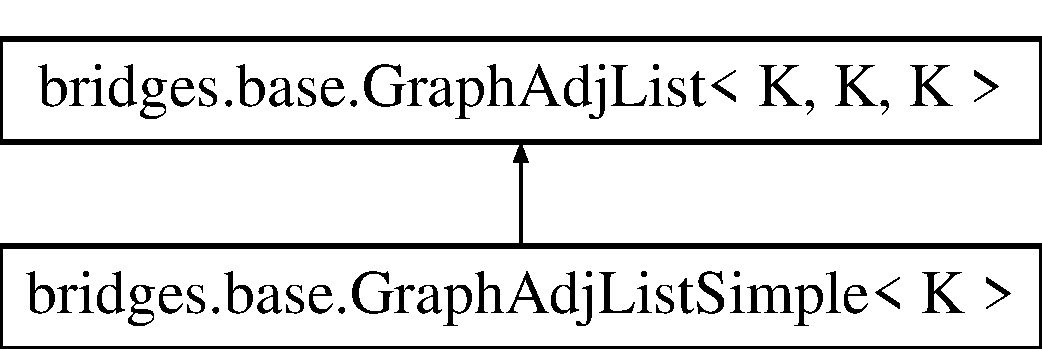
\includegraphics[height=2.000000cm]{classbridges_1_1base_1_1_graph_adj_list_simple}
\end{center}
\end{figure}
\subsection*{Additional Inherited Members}


\subsection{Detailed Description}
The \hyperlink{classbridges_1_1base_1_1_graph_adj_list_simple}{Graph\+Adj\+List\+Simple} class is a simplification of the \hyperlink{classbridges_1_1base_1_1_graph_adj_list}{Graph\+Adj\+List} class; this class is useful in applications where vertex and edge specific information is not used; this class is thus a specialization of \hyperlink{classbridges_1_1base_1_1_graph_adj_list}{Graph\+Adj\+List} with only a single generic parameter that specifies the key type. 

The \hyperlink{classbridges_1_1base_1_1_graph_adj_list_simple}{Graph\+Adj\+List\+Simple} class can be used to represent adjacency list based graphs in B\+R\+I\+D\+G\+E\+S; it takes 1 generic parameter\+: K, which is an orderable key value used in accessing vertices and edges (in constant time) using hashmaps. This permits data sets that need to be accessed by keys that are strings. Vertex and edge specific information can still be represented, but they will be restricted to be of type K.

The class is simply a wrapper around the Java Hashmap class and, thus, derives all its operations from it. B\+R\+I\+D\+G\+E\+S provides methods to visualize the graph and its contents.

The vertices of the graph are held in a Java hashmap, for near constant time access; this lets us use strings or integral ids for vertices. The adjacency lists, also a Java hashmap are built for each vertex and contain the edge (terminating vertex id, weight) in the \hyperlink{classbridges_1_1base_1_1_edge}{Edge} structure, defined separately. Adjacency lists are singly linked lists using the B\+R\+I\+D\+G\+E\+S \hyperlink{classbridges_1_1base_1_1_s_lelement}{S\+Lelement}.

Convenience methods are provided to add vertices and edges to the graph as well as retrieve the adjacency list of a vertex, given its id. Methods to access and set visual attributes are also provided, indexed by the vertex ids.

\begin{DoxyAuthor}{Author}
Kalpathi Subramanian
\end{DoxyAuthor}
\begin{DoxyDate}{Date}
4/24/18
\end{DoxyDate}

\begin{DoxyParams}{Parameters}
{\em $<$\+K$>$} & orderable key (string, int, etc) that is used to index into vertex\\
\hline
\end{DoxyParams}
\begin{DoxySeeAlso}{See also}
Example tutorial at 
\end{DoxySeeAlso}
\href{http://bridgesuncc.github.io/Hello_World_Tutorials/Graph.html}{\tt http\+://bridgesuncc.\+github.\+io/\+Hello\+\_\+\+World\+\_\+\+Tutorials/\+Graph.\+html} 

The documentation for this class was generated from the following file\+:\begin{DoxyCompactItemize}
\item 
/\+Users/kalpathi/gr/bridges/bridges17/java/src/main/java/bridges/base/\hyperlink{_graph_adj_list_simple_8java}{Graph\+Adj\+List\+Simple.\+java}\end{DoxyCompactItemize}

\hypertarget{classbridges_1_1base_1_1_graph_adj_matrix}{}\section{bridges.\+base.\+Graph\+Adj\+Matrix$<$ K, E1, E2 $>$ Class Template Reference}
\label{classbridges_1_1base_1_1_graph_adj_matrix}\index{bridges.\+base.\+Graph\+Adj\+Matrix$<$ K, E1, E2 $>$@{bridges.\+base.\+Graph\+Adj\+Matrix$<$ K, E1, E2 $>$}}
Inheritance diagram for bridges.\+base.\+Graph\+Adj\+Matrix$<$ K, E1, E2 $>$\+:\begin{figure}[H]
\begin{center}
\leavevmode
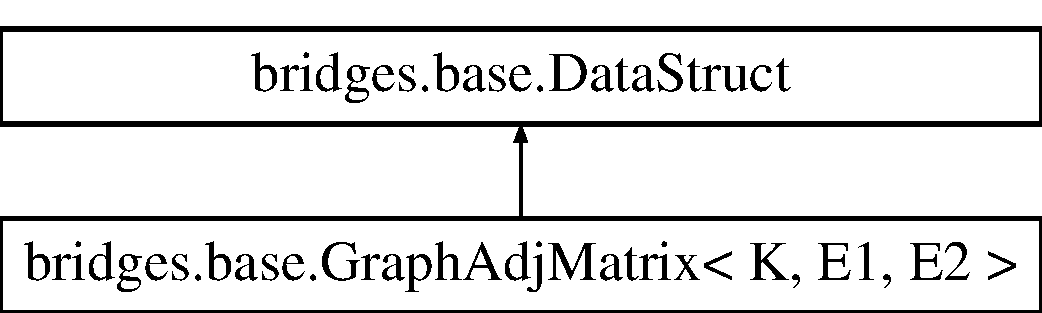
\includegraphics[height=2.000000cm]{classbridges_1_1base_1_1_graph_adj_matrix}
\end{center}
\end{figure}


\subsection{Detailed Description}
The \hyperlink{classbridges_1_1base_1_1_graph_adj_matrix}{Graph\+Adj\+Matrix} class can be used to represent adjacency matrix based graphs in B\+R\+I\+D\+G\+ES. 

The \hyperlink{classbridges_1_1base_1_1_graph_adj_matrix}{Graph\+Adj\+Matrix} class can be used to represent adjacency matrix based graphs in B\+R\+I\+D\+G\+ES; it takes 2 generic parameters\+: (1) K, which is an orderable key value used in accessing vertices (in constant time) using a hashmap. This permits data sets that need to be accessed by keys that are strings, and (2) E, an application defined type, and used in the \hyperlink{classbridges_1_1base_1_1_edge}{Edge} representation. The class is simply a wrapper around the Java Hashmap class and, thus, derives all its operations from it. B\+R\+I\+D\+G\+ES provides methods to visualize the graph and its contents.

The vertices of the graph are held in a Java hashmap, for near constant time access; this lets us use strings or integral ids for vertices. The edges are accessed by a second hashmap from each vertex, again assuring near constant access time. Each edge contains the terminating vertex id and weight, as defined by the \hyperlink{classbridges_1_1base_1_1_edge}{Edge} class structure.

Convenience methods are provided to add vertices and edges to the graph. Edges are retrieved by using the dual hashmap, given the vertex ids of the edge. Methods to access the element and link visualizer are now provided, indexed vertex ids, making it easier to set visual attributes to graph nodes and links.

\begin{DoxySeeAlso}{See also}
Example tutorial at \href{http://bridgesuncc.github.io/tutorials/Graph_AM.html}{\tt http\+://bridgesuncc.\+github.\+io/tutorials/\+Graph\+\_\+\+A\+M.\+html}
\end{DoxySeeAlso}
\begin{DoxyAuthor}{Author}
Kalpathi Subramanian, Mihai Mehedint
\end{DoxyAuthor}
\begin{DoxyDate}{Date}
7/12/15, 5/18/17, 4/23/18
\end{DoxyDate}

\begin{DoxyParams}{Parameters}
{\em K} & orderable key (string, int, etc) that is used to index into vertex \\
\hline
{\em E1} & vertex specific information, for graph vertices \\
\hline
{\em E2} & edge specific information, for graph vertices \\
\hline
\end{DoxyParams}
\subsection*{Public Member Functions}
\begin{DoxyCompactItemize}
\item 
\hyperlink{classbridges_1_1base_1_1_graph_adj_matrix_a8af4a2575890c3e68da7b39d800267bb}{Graph\+Adj\+Matrix} ()
\item 
String \hyperlink{classbridges_1_1base_1_1_graph_adj_matrix_a16ee088c4c53a9a5cdf3fbbad25cd1af}{get\+Data\+Struct\+Type} ()
\item 
void \hyperlink{classbridges_1_1base_1_1_graph_adj_matrix_a27b5ddb10a6615693460955b6bb3ee0c}{add\+Vertex} (K k, E1 e)
\item 
void \hyperlink{classbridges_1_1base_1_1_graph_adj_matrix_a477fbb5abbed6988e67b4b46b571e87c}{add\+Edge} (K src, K dest)
\item 
void \hyperlink{classbridges_1_1base_1_1_graph_adj_matrix_ad9b05b61e9592fa94045d7b59971b206}{add\+Edge} (K src, K dest, int weight)
\item 
void \hyperlink{classbridges_1_1base_1_1_graph_adj_matrix_a22eee632463a665e7016cf50916dfd83}{set\+Vertex\+Data} (K src, E1 vertex\+\_\+data)
\begin{DoxyCompactList}\small\item\em Sets data for a graph vertex. \end{DoxyCompactList}\item 
E1 \hyperlink{classbridges_1_1base_1_1_graph_adj_matrix_a36308a365d1c0f137ffb9a8e76a630f1}{get\+Vertex\+Data} (K src)
\item 
void \hyperlink{classbridges_1_1base_1_1_graph_adj_matrix_a72fe8bd594e3da28ba6e412de88576da}{set\+Edge\+Data} (K src, K dest, E2 data)
\item 
E2 \hyperlink{classbridges_1_1base_1_1_graph_adj_matrix_a3a3795c994ef9033ddb0b1d97029350b}{get\+Edge\+Data} (K src, K dest)
\item 
Hash\+Map$<$ K, \hyperlink{classbridges_1_1base_1_1_element}{Element}$<$ E1 $>$ $>$ \hyperlink{classbridges_1_1base_1_1_graph_adj_matrix_a6a000a302a1082bc2c55fbe8f511fce4}{get\+Vertices} ()
\item 
Hash\+Map$<$ K, Hash\+Map$<$ K, Integer $>$ $>$ \hyperlink{classbridges_1_1base_1_1_graph_adj_matrix_abe7f26cb9874744bc044df18b5d0eb84}{get\+Adjacency\+Matrix} ()
\item 
Hash\+Map$<$ K, Integer $>$ \hyperlink{classbridges_1_1base_1_1_graph_adj_matrix_a43f830cfe126f2be351f6d8c2fccc569}{get\+Adjacency\+Matrix} (K key)
\item 
\hyperlink{classbridges_1_1base_1_1_link_visualizer}{Link\+Visualizer} \hyperlink{classbridges_1_1base_1_1_graph_adj_matrix_a434454a6c8a1fac612392dcf1951dc9d}{get\+Link\+Visualizer} (K src, K dest)  throws Exception 
\item 
\hyperlink{classbridges_1_1base_1_1_element_visualizer}{Element\+Visualizer} \hyperlink{classbridges_1_1base_1_1_graph_adj_matrix_a4358ebee834c69796479a4ee6dfd96b3}{get\+Visualizer} (K vertex)  throws Exception 
\item 
String \hyperlink{classbridges_1_1base_1_1_graph_adj_matrix_ab0786f047bd0c8c47f19d632a1f03eaa}{get\+Data\+Structure\+Representation} ()
\end{DoxyCompactItemize}
\subsection*{Additional Inherited Members}


\subsection{Constructor \& Destructor Documentation}
\mbox{\Hypertarget{classbridges_1_1base_1_1_graph_adj_matrix_a8af4a2575890c3e68da7b39d800267bb}\label{classbridges_1_1base_1_1_graph_adj_matrix_a8af4a2575890c3e68da7b39d800267bb}} 
\index{bridges\+::base\+::\+Graph\+Adj\+Matrix@{bridges\+::base\+::\+Graph\+Adj\+Matrix}!Graph\+Adj\+Matrix@{Graph\+Adj\+Matrix}}
\index{Graph\+Adj\+Matrix@{Graph\+Adj\+Matrix}!bridges\+::base\+::\+Graph\+Adj\+Matrix@{bridges\+::base\+::\+Graph\+Adj\+Matrix}}
\subsubsection{\texorpdfstring{Graph\+Adj\+Matrix()}{GraphAdjMatrix()}}
{\footnotesize\ttfamily \hyperlink{classbridges_1_1base_1_1_graph_adj_matrix}{bridges.\+base.\+Graph\+Adj\+Matrix}$<$ K, E1, E2 $>$.\hyperlink{classbridges_1_1base_1_1_graph_adj_matrix}{Graph\+Adj\+Matrix} (\begin{DoxyParamCaption}{ }\end{DoxyParamCaption})}

Constructor 

\subsection{Member Function Documentation}
\mbox{\Hypertarget{classbridges_1_1base_1_1_graph_adj_matrix_a477fbb5abbed6988e67b4b46b571e87c}\label{classbridges_1_1base_1_1_graph_adj_matrix_a477fbb5abbed6988e67b4b46b571e87c}} 
\index{bridges\+::base\+::\+Graph\+Adj\+Matrix@{bridges\+::base\+::\+Graph\+Adj\+Matrix}!add\+Edge@{add\+Edge}}
\index{add\+Edge@{add\+Edge}!bridges\+::base\+::\+Graph\+Adj\+Matrix@{bridges\+::base\+::\+Graph\+Adj\+Matrix}}
\subsubsection{\texorpdfstring{add\+Edge()}{addEdge()}\hspace{0.1cm}{\footnotesize\ttfamily [1/2]}}
{\footnotesize\ttfamily void \hyperlink{classbridges_1_1base_1_1_graph_adj_matrix}{bridges.\+base.\+Graph\+Adj\+Matrix}$<$ K, E1, E2 $>$.add\+Edge (\begin{DoxyParamCaption}\item[{K}]{src,  }\item[{K}]{dest }\end{DoxyParamCaption})}

Adds a new edge to the graph, adds it to the index corresponding to the source, destination vertex ids; this version of the method assumes an edge weight of 1 (unweighted graph); user is responsible for checking if the vertices already exist, else an exception is thrown.


\begin{DoxyParams}{Parameters}
{\em src} & -\/ source vertex of edge \\
\hline
{\em dest} & -\/ destination vertex of edge \\
\hline
\end{DoxyParams}
\mbox{\Hypertarget{classbridges_1_1base_1_1_graph_adj_matrix_ad9b05b61e9592fa94045d7b59971b206}\label{classbridges_1_1base_1_1_graph_adj_matrix_ad9b05b61e9592fa94045d7b59971b206}} 
\index{bridges\+::base\+::\+Graph\+Adj\+Matrix@{bridges\+::base\+::\+Graph\+Adj\+Matrix}!add\+Edge@{add\+Edge}}
\index{add\+Edge@{add\+Edge}!bridges\+::base\+::\+Graph\+Adj\+Matrix@{bridges\+::base\+::\+Graph\+Adj\+Matrix}}
\subsubsection{\texorpdfstring{add\+Edge()}{addEdge()}\hspace{0.1cm}{\footnotesize\ttfamily [2/2]}}
{\footnotesize\ttfamily void \hyperlink{classbridges_1_1base_1_1_graph_adj_matrix}{bridges.\+base.\+Graph\+Adj\+Matrix}$<$ K, E1, E2 $>$.add\+Edge (\begin{DoxyParamCaption}\item[{K}]{src,  }\item[{K}]{dest,  }\item[{int}]{weight }\end{DoxyParamCaption})}

Adds a new edge of weight \textquotesingle{}weight\textquotesingle{} to the graph, adds it to the index corresponding to the source, destination vertex ids; user is responsible for checking if the vertices already exist, else an exception is thrown.


\begin{DoxyParams}{Parameters}
{\em src} & -\/ source vertex of edge \\
\hline
{\em dest} & -\/ destination vertex of edge \\
\hline
{\em weight} & -\/ edge weight \\
\hline
\end{DoxyParams}
\mbox{\Hypertarget{classbridges_1_1base_1_1_graph_adj_matrix_a27b5ddb10a6615693460955b6bb3ee0c}\label{classbridges_1_1base_1_1_graph_adj_matrix_a27b5ddb10a6615693460955b6bb3ee0c}} 
\index{bridges\+::base\+::\+Graph\+Adj\+Matrix@{bridges\+::base\+::\+Graph\+Adj\+Matrix}!add\+Vertex@{add\+Vertex}}
\index{add\+Vertex@{add\+Vertex}!bridges\+::base\+::\+Graph\+Adj\+Matrix@{bridges\+::base\+::\+Graph\+Adj\+Matrix}}
\subsubsection{\texorpdfstring{add\+Vertex()}{addVertex()}}
{\footnotesize\ttfamily void \hyperlink{classbridges_1_1base_1_1_graph_adj_matrix}{bridges.\+base.\+Graph\+Adj\+Matrix}$<$ K, E1, E2 $>$.add\+Vertex (\begin{DoxyParamCaption}\item[{K}]{k,  }\item[{E1}]{e }\end{DoxyParamCaption})}

Adds a new vertex to the graph, initializes the adjacency list; user is responsible for checking if the vertex already exists. This method will replace the value for this key


\begin{DoxyParams}{Parameters}
{\em k} & -\/ vertex key value \\
\hline
{\em e} & -\/ user specified data, part of the vertex data \\
\hline
\end{DoxyParams}
\mbox{\Hypertarget{classbridges_1_1base_1_1_graph_adj_matrix_abe7f26cb9874744bc044df18b5d0eb84}\label{classbridges_1_1base_1_1_graph_adj_matrix_abe7f26cb9874744bc044df18b5d0eb84}} 
\index{bridges\+::base\+::\+Graph\+Adj\+Matrix@{bridges\+::base\+::\+Graph\+Adj\+Matrix}!get\+Adjacency\+Matrix@{get\+Adjacency\+Matrix}}
\index{get\+Adjacency\+Matrix@{get\+Adjacency\+Matrix}!bridges\+::base\+::\+Graph\+Adj\+Matrix@{bridges\+::base\+::\+Graph\+Adj\+Matrix}}
\subsubsection{\texorpdfstring{get\+Adjacency\+Matrix()}{getAdjacencyMatrix()}\hspace{0.1cm}{\footnotesize\ttfamily [1/2]}}
{\footnotesize\ttfamily Hash\+Map$<$K, Hash\+Map$<$K, Integer$>$ $>$ \hyperlink{classbridges_1_1base_1_1_graph_adj_matrix}{bridges.\+base.\+Graph\+Adj\+Matrix}$<$ K, E1, E2 $>$.get\+Adjacency\+Matrix (\begin{DoxyParamCaption}{ }\end{DoxyParamCaption})}

Gets the adjacency matrix

\begin{DoxyReturn}{Returns}
-\/ the graph\textquotesingle{}s adjacency matrix 
\end{DoxyReturn}
\mbox{\Hypertarget{classbridges_1_1base_1_1_graph_adj_matrix_a43f830cfe126f2be351f6d8c2fccc569}\label{classbridges_1_1base_1_1_graph_adj_matrix_a43f830cfe126f2be351f6d8c2fccc569}} 
\index{bridges\+::base\+::\+Graph\+Adj\+Matrix@{bridges\+::base\+::\+Graph\+Adj\+Matrix}!get\+Adjacency\+Matrix@{get\+Adjacency\+Matrix}}
\index{get\+Adjacency\+Matrix@{get\+Adjacency\+Matrix}!bridges\+::base\+::\+Graph\+Adj\+Matrix@{bridges\+::base\+::\+Graph\+Adj\+Matrix}}
\subsubsection{\texorpdfstring{get\+Adjacency\+Matrix()}{getAdjacencyMatrix()}\hspace{0.1cm}{\footnotesize\ttfamily [2/2]}}
{\footnotesize\ttfamily Hash\+Map$<$K, Integer$>$ \hyperlink{classbridges_1_1base_1_1_graph_adj_matrix}{bridges.\+base.\+Graph\+Adj\+Matrix}$<$ K, E1, E2 $>$.get\+Adjacency\+Matrix (\begin{DoxyParamCaption}\item[{K}]{key }\end{DoxyParamCaption})}

Gets the row of the adjacency matrix corresponding to the key


\begin{DoxyParams}{Parameters}
{\em key} & key value \\
\hline
\end{DoxyParams}
\begin{DoxyReturn}{Returns}
-\/ the graph\textquotesingle{}s adjacency matrix 
\end{DoxyReturn}
\mbox{\Hypertarget{classbridges_1_1base_1_1_graph_adj_matrix_a16ee088c4c53a9a5cdf3fbbad25cd1af}\label{classbridges_1_1base_1_1_graph_adj_matrix_a16ee088c4c53a9a5cdf3fbbad25cd1af}} 
\index{bridges\+::base\+::\+Graph\+Adj\+Matrix@{bridges\+::base\+::\+Graph\+Adj\+Matrix}!get\+Data\+Struct\+Type@{get\+Data\+Struct\+Type}}
\index{get\+Data\+Struct\+Type@{get\+Data\+Struct\+Type}!bridges\+::base\+::\+Graph\+Adj\+Matrix@{bridges\+::base\+::\+Graph\+Adj\+Matrix}}
\subsubsection{\texorpdfstring{get\+Data\+Struct\+Type()}{getDataStructType()}}
{\footnotesize\ttfamily String \hyperlink{classbridges_1_1base_1_1_graph_adj_matrix}{bridges.\+base.\+Graph\+Adj\+Matrix}$<$ K, E1, E2 $>$.get\+Data\+Struct\+Type (\begin{DoxyParamCaption}{ }\end{DoxyParamCaption})}

This method gets the data structure type

\begin{DoxyReturn}{Returns}
The date structure type as a string 
\end{DoxyReturn}
\mbox{\Hypertarget{classbridges_1_1base_1_1_graph_adj_matrix_ab0786f047bd0c8c47f19d632a1f03eaa}\label{classbridges_1_1base_1_1_graph_adj_matrix_ab0786f047bd0c8c47f19d632a1f03eaa}} 
\index{bridges\+::base\+::\+Graph\+Adj\+Matrix@{bridges\+::base\+::\+Graph\+Adj\+Matrix}!get\+Data\+Structure\+Representation@{get\+Data\+Structure\+Representation}}
\index{get\+Data\+Structure\+Representation@{get\+Data\+Structure\+Representation}!bridges\+::base\+::\+Graph\+Adj\+Matrix@{bridges\+::base\+::\+Graph\+Adj\+Matrix}}
\subsubsection{\texorpdfstring{get\+Data\+Structure\+Representation()}{getDataStructureRepresentation()}}
{\footnotesize\ttfamily String \hyperlink{classbridges_1_1base_1_1_graph_adj_matrix}{bridges.\+base.\+Graph\+Adj\+Matrix}$<$ K, E1, E2 $>$.get\+Data\+Structure\+Representation (\begin{DoxyParamCaption}{ }\end{DoxyParamCaption})}

\mbox{\Hypertarget{classbridges_1_1base_1_1_graph_adj_matrix_a3a3795c994ef9033ddb0b1d97029350b}\label{classbridges_1_1base_1_1_graph_adj_matrix_a3a3795c994ef9033ddb0b1d97029350b}} 
\index{bridges\+::base\+::\+Graph\+Adj\+Matrix@{bridges\+::base\+::\+Graph\+Adj\+Matrix}!get\+Edge\+Data@{get\+Edge\+Data}}
\index{get\+Edge\+Data@{get\+Edge\+Data}!bridges\+::base\+::\+Graph\+Adj\+Matrix@{bridges\+::base\+::\+Graph\+Adj\+Matrix}}
\subsubsection{\texorpdfstring{get\+Edge\+Data()}{getEdgeData()}}
{\footnotesize\ttfamily E2 \hyperlink{classbridges_1_1base_1_1_graph_adj_matrix}{bridges.\+base.\+Graph\+Adj\+Matrix}$<$ K, E1, E2 $>$.get\+Edge\+Data (\begin{DoxyParamCaption}\item[{K}]{src,  }\item[{K}]{dest }\end{DoxyParamCaption})}

Gets data for an edge


\begin{DoxyParams}{Parameters}
{\em src} & -\/ source vertex of edge \\
\hline
{\em dest} & -\/ destination vertex of edge \\
\hline
\end{DoxyParams}
\mbox{\Hypertarget{classbridges_1_1base_1_1_graph_adj_matrix_a434454a6c8a1fac612392dcf1951dc9d}\label{classbridges_1_1base_1_1_graph_adj_matrix_a434454a6c8a1fac612392dcf1951dc9d}} 
\index{bridges\+::base\+::\+Graph\+Adj\+Matrix@{bridges\+::base\+::\+Graph\+Adj\+Matrix}!get\+Link\+Visualizer@{get\+Link\+Visualizer}}
\index{get\+Link\+Visualizer@{get\+Link\+Visualizer}!bridges\+::base\+::\+Graph\+Adj\+Matrix@{bridges\+::base\+::\+Graph\+Adj\+Matrix}}
\subsubsection{\texorpdfstring{get\+Link\+Visualizer()}{getLinkVisualizer()}}
{\footnotesize\ttfamily \hyperlink{classbridges_1_1base_1_1_link_visualizer}{Link\+Visualizer} \hyperlink{classbridges_1_1base_1_1_graph_adj_matrix}{bridges.\+base.\+Graph\+Adj\+Matrix}$<$ K, E1, E2 $>$.get\+Link\+Visualizer (\begin{DoxyParamCaption}\item[{K}]{src,  }\item[{K}]{dest }\end{DoxyParamCaption}) throws Exception}

This is a convenience method to simplify access to the link visualizer; the method assumes the vertex names point to existing vertices, else an exception is thrown \mbox{\Hypertarget{classbridges_1_1base_1_1_graph_adj_matrix_a36308a365d1c0f137ffb9a8e76a630f1}\label{classbridges_1_1base_1_1_graph_adj_matrix_a36308a365d1c0f137ffb9a8e76a630f1}} 
\index{bridges\+::base\+::\+Graph\+Adj\+Matrix@{bridges\+::base\+::\+Graph\+Adj\+Matrix}!get\+Vertex\+Data@{get\+Vertex\+Data}}
\index{get\+Vertex\+Data@{get\+Vertex\+Data}!bridges\+::base\+::\+Graph\+Adj\+Matrix@{bridges\+::base\+::\+Graph\+Adj\+Matrix}}
\subsubsection{\texorpdfstring{get\+Vertex\+Data()}{getVertexData()}}
{\footnotesize\ttfamily E1 \hyperlink{classbridges_1_1base_1_1_graph_adj_matrix}{bridges.\+base.\+Graph\+Adj\+Matrix}$<$ K, E1, E2 $>$.get\+Vertex\+Data (\begin{DoxyParamCaption}\item[{K}]{src }\end{DoxyParamCaption})}

Gets data for a vertex


\begin{DoxyParams}{Parameters}
{\em src} & source vertex of edge \\
\hline
\end{DoxyParams}
\mbox{\Hypertarget{classbridges_1_1base_1_1_graph_adj_matrix_a6a000a302a1082bc2c55fbe8f511fce4}\label{classbridges_1_1base_1_1_graph_adj_matrix_a6a000a302a1082bc2c55fbe8f511fce4}} 
\index{bridges\+::base\+::\+Graph\+Adj\+Matrix@{bridges\+::base\+::\+Graph\+Adj\+Matrix}!get\+Vertices@{get\+Vertices}}
\index{get\+Vertices@{get\+Vertices}!bridges\+::base\+::\+Graph\+Adj\+Matrix@{bridges\+::base\+::\+Graph\+Adj\+Matrix}}
\subsubsection{\texorpdfstring{get\+Vertices()}{getVertices()}}
{\footnotesize\ttfamily Hash\+Map$<$K, \hyperlink{classbridges_1_1base_1_1_element}{Element}$<$E1$>$ $>$ \hyperlink{classbridges_1_1base_1_1_graph_adj_matrix}{bridges.\+base.\+Graph\+Adj\+Matrix}$<$ K, E1, E2 $>$.get\+Vertices (\begin{DoxyParamCaption}{ }\end{DoxyParamCaption})}

This method returns the graph nodes 

return -- vertices held in an unordered map \mbox{\Hypertarget{classbridges_1_1base_1_1_graph_adj_matrix_a4358ebee834c69796479a4ee6dfd96b3}\label{classbridges_1_1base_1_1_graph_adj_matrix_a4358ebee834c69796479a4ee6dfd96b3}} 
\index{bridges\+::base\+::\+Graph\+Adj\+Matrix@{bridges\+::base\+::\+Graph\+Adj\+Matrix}!get\+Visualizer@{get\+Visualizer}}
\index{get\+Visualizer@{get\+Visualizer}!bridges\+::base\+::\+Graph\+Adj\+Matrix@{bridges\+::base\+::\+Graph\+Adj\+Matrix}}
\subsubsection{\texorpdfstring{get\+Visualizer()}{getVisualizer()}}
{\footnotesize\ttfamily \hyperlink{classbridges_1_1base_1_1_element_visualizer}{Element\+Visualizer} \hyperlink{classbridges_1_1base_1_1_graph_adj_matrix}{bridges.\+base.\+Graph\+Adj\+Matrix}$<$ K, E1, E2 $>$.get\+Visualizer (\begin{DoxyParamCaption}\item[{K}]{vertex }\end{DoxyParamCaption}) throws Exception}

This is a convenience method to simplify access to the element visualizer; the method assumes the vertex name points to an existing vertice, else an exception is thrown \mbox{\Hypertarget{classbridges_1_1base_1_1_graph_adj_matrix_a72fe8bd594e3da28ba6e412de88576da}\label{classbridges_1_1base_1_1_graph_adj_matrix_a72fe8bd594e3da28ba6e412de88576da}} 
\index{bridges\+::base\+::\+Graph\+Adj\+Matrix@{bridges\+::base\+::\+Graph\+Adj\+Matrix}!set\+Edge\+Data@{set\+Edge\+Data}}
\index{set\+Edge\+Data@{set\+Edge\+Data}!bridges\+::base\+::\+Graph\+Adj\+Matrix@{bridges\+::base\+::\+Graph\+Adj\+Matrix}}
\subsubsection{\texorpdfstring{set\+Edge\+Data()}{setEdgeData()}}
{\footnotesize\ttfamily void \hyperlink{classbridges_1_1base_1_1_graph_adj_matrix}{bridges.\+base.\+Graph\+Adj\+Matrix}$<$ K, E1, E2 $>$.set\+Edge\+Data (\begin{DoxyParamCaption}\item[{K}]{src,  }\item[{K}]{dest,  }\item[{E2}]{data }\end{DoxyParamCaption})}

Sets data for an edge


\begin{DoxyParams}{Parameters}
{\em src} & -\/ source vertex of edge \\
\hline
{\em dest} & -\/ destination vertex of edge \\
\hline
{\em data} & -\/ edge data \\
\hline
\end{DoxyParams}
\mbox{\Hypertarget{classbridges_1_1base_1_1_graph_adj_matrix_a22eee632463a665e7016cf50916dfd83}\label{classbridges_1_1base_1_1_graph_adj_matrix_a22eee632463a665e7016cf50916dfd83}} 
\index{bridges\+::base\+::\+Graph\+Adj\+Matrix@{bridges\+::base\+::\+Graph\+Adj\+Matrix}!set\+Vertex\+Data@{set\+Vertex\+Data}}
\index{set\+Vertex\+Data@{set\+Vertex\+Data}!bridges\+::base\+::\+Graph\+Adj\+Matrix@{bridges\+::base\+::\+Graph\+Adj\+Matrix}}
\subsubsection{\texorpdfstring{set\+Vertex\+Data()}{setVertexData()}}
{\footnotesize\ttfamily void \hyperlink{classbridges_1_1base_1_1_graph_adj_matrix}{bridges.\+base.\+Graph\+Adj\+Matrix}$<$ K, E1, E2 $>$.set\+Vertex\+Data (\begin{DoxyParamCaption}\item[{K}]{src,  }\item[{E1}]{vertex\+\_\+data }\end{DoxyParamCaption})}



Sets data for a graph vertex. 


\begin{DoxyParams}{Parameters}
{\em src} & source vertex of edge \\
\hline
{\em vertex\+\_\+data} & vertex data \\
\hline
\end{DoxyParams}


The documentation for this class was generated from the following file\+:\begin{DoxyCompactItemize}
\item 
/home/erik/work/bridges/bridges-\/java/src/main/java/bridges/base/\hyperlink{_graph_adj_matrix_8java}{Graph\+Adj\+Matrix.\+java}\end{DoxyCompactItemize}

\hypertarget{classbridges_1_1base_1_1_graph_adj_matrix_simple}{}\section{bridges.\+base.\+Graph\+Adj\+Matrix\+Simple$<$ K $>$ Class Template Reference}
\label{classbridges_1_1base_1_1_graph_adj_matrix_simple}\index{bridges.\+base.\+Graph\+Adj\+Matrix\+Simple$<$ K $>$@{bridges.\+base.\+Graph\+Adj\+Matrix\+Simple$<$ K $>$}}


The \mbox{\hyperlink{classbridges_1_1base_1_1_graph_adj_matrix_simple}{Graph\+Adj\+Matrix\+Simple}} class is a simplification of the \mbox{\hyperlink{classbridges_1_1base_1_1_graph_adj_matrix}{Graph\+Adj\+Matrix}} class; this class is useful in applications where vertex and edge specific information is not used; this class is thus a specialization of \mbox{\hyperlink{classbridges_1_1base_1_1_graph_adj_list}{Graph\+Adj\+List}} with only a single generic parameter that specifies the key type.  


Inheritance diagram for bridges.\+base.\+Graph\+Adj\+Matrix\+Simple$<$ K $>$\+:\begin{figure}[H]
\begin{center}
\leavevmode
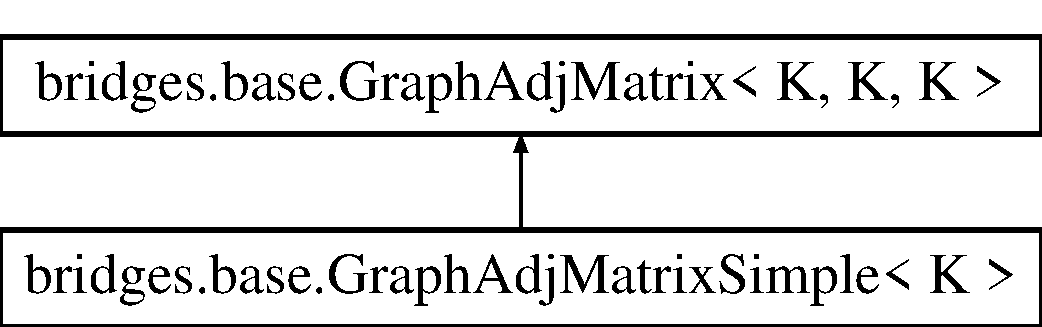
\includegraphics[height=2.000000cm]{classbridges_1_1base_1_1_graph_adj_matrix_simple}
\end{center}
\end{figure}
\subsection*{Additional Inherited Members}


\subsection{Detailed Description}
The \mbox{\hyperlink{classbridges_1_1base_1_1_graph_adj_matrix_simple}{Graph\+Adj\+Matrix\+Simple}} class is a simplification of the \mbox{\hyperlink{classbridges_1_1base_1_1_graph_adj_matrix}{Graph\+Adj\+Matrix}} class; this class is useful in applications where vertex and edge specific information is not used; this class is thus a specialization of \mbox{\hyperlink{classbridges_1_1base_1_1_graph_adj_list}{Graph\+Adj\+List}} with only a single generic parameter that specifies the key type. 

The \mbox{\hyperlink{classbridges_1_1base_1_1_graph_adj_matrix_simple}{Graph\+Adj\+Matrix\+Simple}} class can be used to represent adjacency list based ~\newline
graphs in B\+R\+I\+D\+G\+ES; it takes 1 generic parameter\+: K, which is an orderable key value used in accessing vertices and edges (in constant time) using hashmaps. This permits data sets that need to be accessed by keys that are strings. Vertex and edge specific information can still be represented, but they will be restricted to be of type K.

The class is simply a wrapper around the Java Hashmap class and, thus, derives all its operations from it. B\+R\+I\+D\+G\+ES provides methods to visualize the graph and its contents.

The vertices of the graph are held in a Java hashmap of hashmaps(2\+D hashmap), for near constant time access; this lets us use strings or integral ids for vertices. \mbox{\hyperlink{classbridges_1_1base_1_1_edge}{Edge}} information is also held in a hashmap with accessor methods.

Convenience methods are provided to add vertices and edges to the graph as well as retrieve the adjacency list of a vertex, given its id. Methods to access and set visual attributes are also provided, indexed by the vertex ids.

\begin{DoxyAuthor}{Author}
Kalpathi Subramanian
\end{DoxyAuthor}
\begin{DoxyDate}{Date}
4/24/18
\end{DoxyDate}

\begin{DoxyParams}{Parameters}
{\em $<$\+K$>$} & orderable key (string, int, etc) that is used to index into vertex\\
\hline
\end{DoxyParams}
\begin{DoxySeeAlso}{See also}
Example tutorial at 
\end{DoxySeeAlso}
\href{http://bridgesuncc.github.io/Hello_World_Tutorials/Graph.html}{\tt http\+://bridgesuncc.\+github.\+io/\+Hello\+\_\+\+World\+\_\+\+Tutorials/\+Graph.\+html} 

The documentation for this class was generated from the following file\+:\begin{DoxyCompactItemize}
\item 
/\+Users/kalpathi/gr/bridges/client/java/bridges-\/17/src/main/java/edu/uncc/cs/bridges\+\_\+v21/base/\mbox{\hyperlink{_graph_adj_matrix_simple_8java}{Graph\+Adj\+Matrix\+Simple.\+java}}\end{DoxyCompactItemize}

\hypertarget{classbridges_1_1base_1_1_grid}{}\section{bridges.\+base.\+Grid$<$ E $>$ Class Template Reference}
\label{classbridges_1_1base_1_1_grid}\index{bridges.\+base.\+Grid$<$ E $>$@{bridges.\+base.\+Grid$<$ E $>$}}
Inheritance diagram for bridges.\+base.\+Grid$<$ E $>$\+:\begin{figure}[H]
\begin{center}
\leavevmode
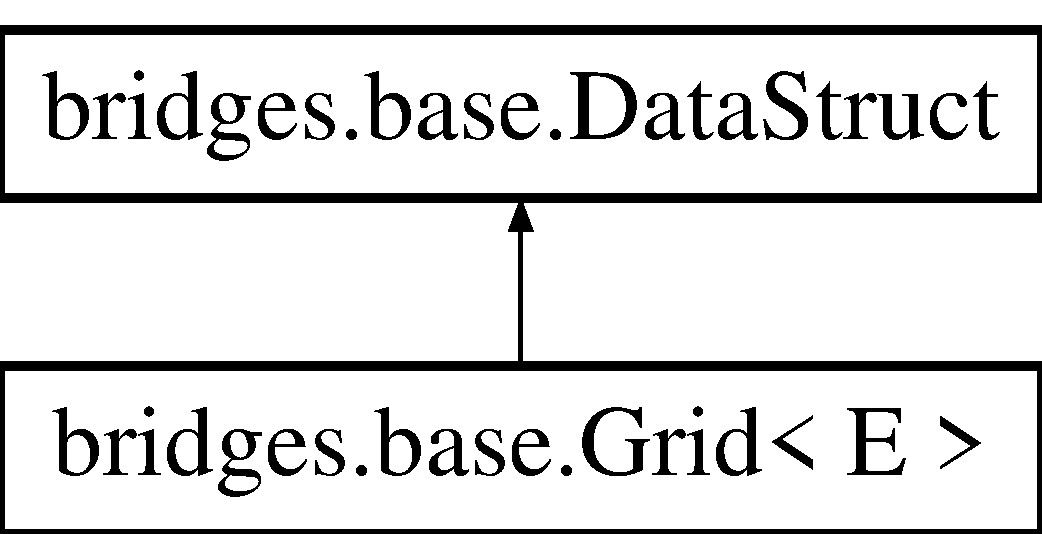
\includegraphics[height=2.000000cm]{classbridges_1_1base_1_1_grid}
\end{center}
\end{figure}


\subsection{Detailed Description}
This is a class in B\+R\+I\+D\+G\+ES for representing an (m x n) grid. 

\begin{DoxyAuthor}{Author}
David Burlinson 
\end{DoxyAuthor}
\begin{DoxyDate}{Date}
5/14/18, 7/14/19 
\end{DoxyDate}
\subsection*{Public Member Functions}
\begin{DoxyCompactItemize}
\item 
String \mbox{\hyperlink{classbridges_1_1base_1_1_grid_a81f268dd27c292ff2af9358039d4ebe6}{get\+Data\+Struct\+Type}} ()
\item 
\mbox{\hyperlink{classbridges_1_1base_1_1_grid_aa621ffc958db8341f7ce37ed78944d51}{Grid}} ()
\item 
\mbox{\hyperlink{classbridges_1_1base_1_1_grid_a9818d4959813f1292c6a234bc6f6aa9e}{Grid}} (int size)
\item 
\mbox{\hyperlink{classbridges_1_1base_1_1_grid_a43a699bd7ae2c6c986f978c515ff97d8}{Grid}} (int rows, int cols)
\item 
\mbox{\hyperlink{classbridges_1_1base_1_1_grid_ab9975b28d8dda7f3fbe0e35a7a026772}{Grid}} (int\mbox{[}$\,$\mbox{]} size)
\item 
int \mbox{[}$\,$\mbox{]} \mbox{\hyperlink{classbridges_1_1base_1_1_grid_aee8a5b66095d65ff067a4e76f2611b0e}{get\+Dimensions}} ()
\item 
E \mbox{\hyperlink{classbridges_1_1base_1_1_grid_a698579bb5b7166f76a18a1b04916e090}{get}} (Integer row, Integer col)
\item 
void \mbox{\hyperlink{classbridges_1_1base_1_1_grid_ab79ceb737423bb28ea2348e61a625a17}{set}} (Integer row, Integer col, E val)
\item 
String \mbox{\hyperlink{classbridges_1_1base_1_1_grid_a9a7faf2bbabae8d2f2babe9e29deb2c8}{get\+Data\+Structure\+Representation}} ()
\end{DoxyCompactItemize}
\subsection*{Protected Attributes}
\begin{DoxyCompactItemize}
\item 
Array\+List$<$ Array\+List$<$ E $>$ $>$ \mbox{\hyperlink{classbridges_1_1base_1_1_grid_ad1f3f6968d58188425bd992c05c655a6}{grid}}
\item 
int \mbox{[}$\,$\mbox{]} \mbox{\hyperlink{classbridges_1_1base_1_1_grid_a54a66479f78022570253d771206a0420}{grid\+Size}}
\end{DoxyCompactItemize}
\subsection*{Static Protected Attributes}
\begin{DoxyCompactItemize}
\item 
static final int \mbox{[}$\,$\mbox{]} \mbox{\hyperlink{classbridges_1_1base_1_1_grid_a45c2786d2af83624202192857a27724f}{default\+Grid\+Size}} = \{10, 10\}
\item 
static int \mbox{[}$\,$\mbox{]} \mbox{\hyperlink{classbridges_1_1base_1_1_grid_a803fd4c070a22863c82581f0bb258c1c}{max\+Grid\+Size}} = \{1080, 1920\}
\end{DoxyCompactItemize}


\subsection{Constructor \& Destructor Documentation}
\mbox{\Hypertarget{classbridges_1_1base_1_1_grid_aa621ffc958db8341f7ce37ed78944d51}\label{classbridges_1_1base_1_1_grid_aa621ffc958db8341f7ce37ed78944d51}} 
\index{bridges\+::base\+::\+Grid@{bridges\+::base\+::\+Grid}!Grid@{Grid}}
\index{Grid@{Grid}!bridges\+::base\+::\+Grid@{bridges\+::base\+::\+Grid}}
\subsubsection{\texorpdfstring{Grid()}{Grid()}\hspace{0.1cm}{\footnotesize\ttfamily [1/4]}}
{\footnotesize\ttfamily \mbox{\hyperlink{classbridges_1_1base_1_1_grid}{bridges.\+base.\+Grid}}$<$ E $>$.\mbox{\hyperlink{classbridges_1_1base_1_1_grid}{Grid}} (\begin{DoxyParamCaption}{ }\end{DoxyParamCaption})}

Construct a grid with default sizes \mbox{\Hypertarget{classbridges_1_1base_1_1_grid_a9818d4959813f1292c6a234bc6f6aa9e}\label{classbridges_1_1base_1_1_grid_a9818d4959813f1292c6a234bc6f6aa9e}} 
\index{bridges\+::base\+::\+Grid@{bridges\+::base\+::\+Grid}!Grid@{Grid}}
\index{Grid@{Grid}!bridges\+::base\+::\+Grid@{bridges\+::base\+::\+Grid}}
\subsubsection{\texorpdfstring{Grid()}{Grid()}\hspace{0.1cm}{\footnotesize\ttfamily [2/4]}}
{\footnotesize\ttfamily \mbox{\hyperlink{classbridges_1_1base_1_1_grid}{bridges.\+base.\+Grid}}$<$ E $>$.\mbox{\hyperlink{classbridges_1_1base_1_1_grid}{Grid}} (\begin{DoxyParamCaption}\item[{int}]{size }\end{DoxyParamCaption})}

Construct a size x size grid \mbox{\Hypertarget{classbridges_1_1base_1_1_grid_a43a699bd7ae2c6c986f978c515ff97d8}\label{classbridges_1_1base_1_1_grid_a43a699bd7ae2c6c986f978c515ff97d8}} 
\index{bridges\+::base\+::\+Grid@{bridges\+::base\+::\+Grid}!Grid@{Grid}}
\index{Grid@{Grid}!bridges\+::base\+::\+Grid@{bridges\+::base\+::\+Grid}}
\subsubsection{\texorpdfstring{Grid()}{Grid()}\hspace{0.1cm}{\footnotesize\ttfamily [3/4]}}
{\footnotesize\ttfamily \mbox{\hyperlink{classbridges_1_1base_1_1_grid}{bridges.\+base.\+Grid}}$<$ E $>$.\mbox{\hyperlink{classbridges_1_1base_1_1_grid}{Grid}} (\begin{DoxyParamCaption}\item[{int}]{rows,  }\item[{int}]{cols }\end{DoxyParamCaption})}

Construct a rows x cols size grid


\begin{DoxyParams}{Parameters}
{\em rows} & number of rows in grid \\
\hline
{\em cols} & number of rows in grid \\
\hline
\end{DoxyParams}
\mbox{\Hypertarget{classbridges_1_1base_1_1_grid_ab9975b28d8dda7f3fbe0e35a7a026772}\label{classbridges_1_1base_1_1_grid_ab9975b28d8dda7f3fbe0e35a7a026772}} 
\index{bridges\+::base\+::\+Grid@{bridges\+::base\+::\+Grid}!Grid@{Grid}}
\index{Grid@{Grid}!bridges\+::base\+::\+Grid@{bridges\+::base\+::\+Grid}}
\subsubsection{\texorpdfstring{Grid()}{Grid()}\hspace{0.1cm}{\footnotesize\ttfamily [4/4]}}
{\footnotesize\ttfamily \mbox{\hyperlink{classbridges_1_1base_1_1_grid}{bridges.\+base.\+Grid}}$<$ E $>$.\mbox{\hyperlink{classbridges_1_1base_1_1_grid}{Grid}} (\begin{DoxyParamCaption}\item[{int \mbox{[}$\,$\mbox{]}}]{size }\end{DoxyParamCaption})}

Construct a size\mbox{[}0\mbox{]} by size\mbox{[}1\mbox{]} sized grid 
\begin{DoxyParams}{Parameters}
{\em size\mbox{[}$\,$\mbox{]}} & specifies rows and column sizes of the grid \\
\hline
\end{DoxyParams}


\subsection{Member Function Documentation}
\mbox{\Hypertarget{classbridges_1_1base_1_1_grid_a698579bb5b7166f76a18a1b04916e090}\label{classbridges_1_1base_1_1_grid_a698579bb5b7166f76a18a1b04916e090}} 
\index{bridges\+::base\+::\+Grid@{bridges\+::base\+::\+Grid}!get@{get}}
\index{get@{get}!bridges\+::base\+::\+Grid@{bridges\+::base\+::\+Grid}}
\subsubsection{\texorpdfstring{get()}{get()}}
{\footnotesize\ttfamily E \mbox{\hyperlink{classbridges_1_1base_1_1_grid}{bridges.\+base.\+Grid}}$<$ E $>$.get (\begin{DoxyParamCaption}\item[{Integer}]{row,  }\item[{Integer}]{col }\end{DoxyParamCaption})}

Get the (row, col) element in the grid 
\begin{DoxyParams}{Parameters}
{\em row} & row number \\
\hline
{\em col} & number \\
\hline
\end{DoxyParams}
\mbox{\Hypertarget{classbridges_1_1base_1_1_grid_a81f268dd27c292ff2af9358039d4ebe6}\label{classbridges_1_1base_1_1_grid_a81f268dd27c292ff2af9358039d4ebe6}} 
\index{bridges\+::base\+::\+Grid@{bridges\+::base\+::\+Grid}!get\+Data\+Struct\+Type@{get\+Data\+Struct\+Type}}
\index{get\+Data\+Struct\+Type@{get\+Data\+Struct\+Type}!bridges\+::base\+::\+Grid@{bridges\+::base\+::\+Grid}}
\subsubsection{\texorpdfstring{get\+Data\+Struct\+Type()}{getDataStructType()}}
{\footnotesize\ttfamily String \mbox{\hyperlink{classbridges_1_1base_1_1_grid}{bridges.\+base.\+Grid}}$<$ E $>$.get\+Data\+Struct\+Type (\begin{DoxyParamCaption}{ }\end{DoxyParamCaption})}

Get data structure name \begin{DoxyReturn}{Returns}
data type name 
\end{DoxyReturn}
\mbox{\Hypertarget{classbridges_1_1base_1_1_grid_a9a7faf2bbabae8d2f2babe9e29deb2c8}\label{classbridges_1_1base_1_1_grid_a9a7faf2bbabae8d2f2babe9e29deb2c8}} 
\index{bridges\+::base\+::\+Grid@{bridges\+::base\+::\+Grid}!get\+Data\+Structure\+Representation@{get\+Data\+Structure\+Representation}}
\index{get\+Data\+Structure\+Representation@{get\+Data\+Structure\+Representation}!bridges\+::base\+::\+Grid@{bridges\+::base\+::\+Grid}}
\subsubsection{\texorpdfstring{get\+Data\+Structure\+Representation()}{getDataStructureRepresentation()}}
{\footnotesize\ttfamily String \mbox{\hyperlink{classbridges_1_1base_1_1_grid}{bridges.\+base.\+Grid}}$<$ E $>$.get\+Data\+Structure\+Representation (\begin{DoxyParamCaption}{ }\end{DoxyParamCaption})}

Get data structure representation \mbox{\Hypertarget{classbridges_1_1base_1_1_grid_aee8a5b66095d65ff067a4e76f2611b0e}\label{classbridges_1_1base_1_1_grid_aee8a5b66095d65ff067a4e76f2611b0e}} 
\index{bridges\+::base\+::\+Grid@{bridges\+::base\+::\+Grid}!get\+Dimensions@{get\+Dimensions}}
\index{get\+Dimensions@{get\+Dimensions}!bridges\+::base\+::\+Grid@{bridges\+::base\+::\+Grid}}
\subsubsection{\texorpdfstring{get\+Dimensions()}{getDimensions()}}
{\footnotesize\ttfamily int \mbox{[}$\,$\mbox{]} \mbox{\hyperlink{classbridges_1_1base_1_1_grid}{bridges.\+base.\+Grid}}$<$ E $>$.get\+Dimensions (\begin{DoxyParamCaption}{ }\end{DoxyParamCaption})}

Get the grid dimensions

\begin{DoxyReturn}{Returns}
an array of two values (rows, cols) of the grid 
\end{DoxyReturn}
\mbox{\Hypertarget{classbridges_1_1base_1_1_grid_ab79ceb737423bb28ea2348e61a625a17}\label{classbridges_1_1base_1_1_grid_ab79ceb737423bb28ea2348e61a625a17}} 
\index{bridges\+::base\+::\+Grid@{bridges\+::base\+::\+Grid}!set@{set}}
\index{set@{set}!bridges\+::base\+::\+Grid@{bridges\+::base\+::\+Grid}}
\subsubsection{\texorpdfstring{set()}{set()}}
{\footnotesize\ttfamily void \mbox{\hyperlink{classbridges_1_1base_1_1_grid}{bridges.\+base.\+Grid}}$<$ E $>$.set (\begin{DoxyParamCaption}\item[{Integer}]{row,  }\item[{Integer}]{col,  }\item[{E}]{val }\end{DoxyParamCaption})}

Set the (row, col) element in the grid 
\begin{DoxyParams}{Parameters}
{\em row,col} & cell to change \\
\hline
{\em val} & the value to be set to \\
\hline
\end{DoxyParams}


\subsection{Member Data Documentation}
\mbox{\Hypertarget{classbridges_1_1base_1_1_grid_a45c2786d2af83624202192857a27724f}\label{classbridges_1_1base_1_1_grid_a45c2786d2af83624202192857a27724f}} 
\index{bridges\+::base\+::\+Grid@{bridges\+::base\+::\+Grid}!default\+Grid\+Size@{default\+Grid\+Size}}
\index{default\+Grid\+Size@{default\+Grid\+Size}!bridges\+::base\+::\+Grid@{bridges\+::base\+::\+Grid}}
\subsubsection{\texorpdfstring{default\+Grid\+Size}{defaultGridSize}}
{\footnotesize\ttfamily final int \mbox{[}$\,$\mbox{]} \mbox{\hyperlink{classbridges_1_1base_1_1_grid}{bridges.\+base.\+Grid}}$<$ E $>$.default\+Grid\+Size = \{10, 10\}\hspace{0.3cm}{\ttfamily [static]}, {\ttfamily [protected]}}

\mbox{\Hypertarget{classbridges_1_1base_1_1_grid_ad1f3f6968d58188425bd992c05c655a6}\label{classbridges_1_1base_1_1_grid_ad1f3f6968d58188425bd992c05c655a6}} 
\index{bridges\+::base\+::\+Grid@{bridges\+::base\+::\+Grid}!grid@{grid}}
\index{grid@{grid}!bridges\+::base\+::\+Grid@{bridges\+::base\+::\+Grid}}
\subsubsection{\texorpdfstring{grid}{grid}}
{\footnotesize\ttfamily Array\+List$<$Array\+List$<$E$>$ $>$ \mbox{\hyperlink{classbridges_1_1base_1_1_grid}{bridges.\+base.\+Grid}}$<$ E $>$.grid\hspace{0.3cm}{\ttfamily [protected]}}

\mbox{\Hypertarget{classbridges_1_1base_1_1_grid_a54a66479f78022570253d771206a0420}\label{classbridges_1_1base_1_1_grid_a54a66479f78022570253d771206a0420}} 
\index{bridges\+::base\+::\+Grid@{bridges\+::base\+::\+Grid}!grid\+Size@{grid\+Size}}
\index{grid\+Size@{grid\+Size}!bridges\+::base\+::\+Grid@{bridges\+::base\+::\+Grid}}
\subsubsection{\texorpdfstring{grid\+Size}{gridSize}}
{\footnotesize\ttfamily int \mbox{[}$\,$\mbox{]} \mbox{\hyperlink{classbridges_1_1base_1_1_grid}{bridges.\+base.\+Grid}}$<$ E $>$.grid\+Size\hspace{0.3cm}{\ttfamily [protected]}}

\mbox{\Hypertarget{classbridges_1_1base_1_1_grid_a803fd4c070a22863c82581f0bb258c1c}\label{classbridges_1_1base_1_1_grid_a803fd4c070a22863c82581f0bb258c1c}} 
\index{bridges\+::base\+::\+Grid@{bridges\+::base\+::\+Grid}!max\+Grid\+Size@{max\+Grid\+Size}}
\index{max\+Grid\+Size@{max\+Grid\+Size}!bridges\+::base\+::\+Grid@{bridges\+::base\+::\+Grid}}
\subsubsection{\texorpdfstring{max\+Grid\+Size}{maxGridSize}}
{\footnotesize\ttfamily int \mbox{[}$\,$\mbox{]} \mbox{\hyperlink{classbridges_1_1base_1_1_grid}{bridges.\+base.\+Grid}}$<$ E $>$.max\+Grid\+Size = \{1080, 1920\}\hspace{0.3cm}{\ttfamily [static]}, {\ttfamily [protected]}}



The documentation for this class was generated from the following file\+:\begin{DoxyCompactItemize}
\item 
/\+Users/kalpathi/gr/bridges/client/java/src/main/java/bridges/base/\mbox{\hyperlink{_grid_8java}{Grid.\+java}}\end{DoxyCompactItemize}

\hypertarget{classbridges_1_1data__src__dependent_1_1_gutenberg_book}{}\section{bridges.\+data\+\_\+src\+\_\+dependent.\+Gutenberg\+Book Class Reference}
\label{classbridges_1_1data__src__dependent_1_1_gutenberg_book}\index{bridges.\+data\+\_\+src\+\_\+dependent.\+Gutenberg\+Book@{bridges.\+data\+\_\+src\+\_\+dependent.\+Gutenberg\+Book}}


Inherits bridges.\+data\+\_\+src\+\_\+dependent.\+Data\+Source.

\subsection*{Public Member Functions}
\begin{DoxyCompactItemize}
\item 
\hyperlink{classbridges_1_1data__src__dependent_1_1_gutenberg_book_a34e237fe23613dad17e4b5e005077927}{Gutenberg\+Book} ()
\item 
\hyperlink{classbridges_1_1data__src__dependent_1_1_gutenberg_book_ab35292d8e1464ce388326cafe29ed713}{Gutenberg\+Book} (String author\+Name, int author\+Birth, int author\+Death, String title, Vector$<$ String $>$ languages, Vector$<$ String $>$ genre, Vector$<$ String $>$ subjects, int num\+Chars, int num\+Words, int num\+Sentences, int num\+Difficult\+Words, String url, int downloads)
\item 
String \hyperlink{classbridges_1_1data__src__dependent_1_1_gutenberg_book_a8f66ba5bea27dbecb1658add3a278e45}{get\+Author\+Name} ()
\item 
void \hyperlink{classbridges_1_1data__src__dependent_1_1_gutenberg_book_a6d6e1ccac0fc2e0b09aa6ac6fbe727bc}{set\+Author\+Name} (String author\+Name)
\item 
int \hyperlink{classbridges_1_1data__src__dependent_1_1_gutenberg_book_a00e6f487af339abaa5eb83d315abc3c6}{get\+Author\+Birth} ()
\item 
void \hyperlink{classbridges_1_1data__src__dependent_1_1_gutenberg_book_ad54dbb22312e98761ae3d19f3b94ff85}{set\+Author\+Birth} (int author\+Birth)
\item 
int \hyperlink{classbridges_1_1data__src__dependent_1_1_gutenberg_book_aa1b308207d35f65ceaf85a6bc919d0da}{get\+Author\+Death} ()
\item 
void \hyperlink{classbridges_1_1data__src__dependent_1_1_gutenberg_book_af9aef84c74d681c1a41cbc37698ced18}{set\+Author\+Death} (int author\+Death)
\item 
String \hyperlink{classbridges_1_1data__src__dependent_1_1_gutenberg_book_ae2d9bc547f329c9e6cc862e275b11f21}{get\+Title} ()
\item 
void \hyperlink{classbridges_1_1data__src__dependent_1_1_gutenberg_book_a1f4b11121296e76e4d5afc86157b52d4}{set\+Title} (String title)
\item 
Vector$<$ String $>$ \hyperlink{classbridges_1_1data__src__dependent_1_1_gutenberg_book_a75fffcba3f25be92c02fda1d42c9bcc4}{get\+Languages} ()
\item 
void \hyperlink{classbridges_1_1data__src__dependent_1_1_gutenberg_book_aa201ecea7ae505f66bd97ad7a18c7729}{set\+Languages} (Vector$<$ String $>$ languages)
\item 
Vector$<$ String $>$ \hyperlink{classbridges_1_1data__src__dependent_1_1_gutenberg_book_a7b703adfeef0bd494d1a17ac54b058ce}{get\+Genres} ()
\item 
void \hyperlink{classbridges_1_1data__src__dependent_1_1_gutenberg_book_a76bf1d07025029f0cc9443a6d3d5a956}{set\+Genres} (Vector$<$ String $>$ genre)
\item 
Vector$<$ String $>$ \hyperlink{classbridges_1_1data__src__dependent_1_1_gutenberg_book_a2cc3e828698852aec79279857e519478}{get\+Subjects} ()
\item 
void \hyperlink{classbridges_1_1data__src__dependent_1_1_gutenberg_book_a01c0c69770b1e58b8271f50a4bdf2966}{set\+Subjects} (Vector$<$ String $>$ subjects)
\item 
String \hyperlink{classbridges_1_1data__src__dependent_1_1_gutenberg_book_a7706b211a1acd2a1672d560907eea908}{get\+U\+R\+L} ()
\item 
void \hyperlink{classbridges_1_1data__src__dependent_1_1_gutenberg_book_a9069f9c6835df30ccabf179158b9aa18}{set\+U\+R\+L} (String url)
\item 
int \hyperlink{classbridges_1_1data__src__dependent_1_1_gutenberg_book_a232d5410eaef5ef75208d42a5125a363}{get\+Num\+Chars} ()
\item 
void \hyperlink{classbridges_1_1data__src__dependent_1_1_gutenberg_book_a3f5553b807a6a4f0f97d15b615344159}{set\+Num\+Chars} (int num\+Chars)
\item 
int \hyperlink{classbridges_1_1data__src__dependent_1_1_gutenberg_book_adf4daf7ef5446856d17749698bfec2a2}{get\+Num\+Words} ()
\item 
void \hyperlink{classbridges_1_1data__src__dependent_1_1_gutenberg_book_af84b3422dbb558aa08ff1b40c0068c87}{set\+Num\+Words} (int num\+Words)
\item 
int \hyperlink{classbridges_1_1data__src__dependent_1_1_gutenberg_book_a0d42fd351ee8b2861e43b6c4aad2bca1}{get\+Num\+Sentences} ()
\item 
void \hyperlink{classbridges_1_1data__src__dependent_1_1_gutenberg_book_a3690d6d74f3f47aa8a0fbc4d57f3102a}{set\+Num\+Sentences} (int num\+Sentences)
\item 
int \hyperlink{classbridges_1_1data__src__dependent_1_1_gutenberg_book_ad73c847c8f4c2ce0873b2f14ae6af704}{get\+Num\+Difficult\+Words} ()
\item 
void \hyperlink{classbridges_1_1data__src__dependent_1_1_gutenberg_book_a3b817aed71eab713aad3afe6f02ef3ed}{set\+Num\+Difficult\+Words} (int num\+Difficult\+Words)
\item 
int \hyperlink{classbridges_1_1data__src__dependent_1_1_gutenberg_book_ab15136957384a78824d9a1bccdc41fd5}{get\+Num\+Downloads} ()
\item 
void \hyperlink{classbridges_1_1data__src__dependent_1_1_gutenberg_book_aa871c9aa9a34d7de8409c1c0f24c3dbe}{set\+Num\+Downloads} (int dl)
\end{DoxyCompactItemize}


\subsection{Constructor \& Destructor Documentation}
\hypertarget{classbridges_1_1data__src__dependent_1_1_gutenberg_book_a34e237fe23613dad17e4b5e005077927}{}\index{bridges\+::data\+\_\+src\+\_\+dependent\+::\+Gutenberg\+Book@{bridges\+::data\+\_\+src\+\_\+dependent\+::\+Gutenberg\+Book}!Gutenberg\+Book@{Gutenberg\+Book}}
\index{Gutenberg\+Book@{Gutenberg\+Book}!bridges\+::data\+\_\+src\+\_\+dependent\+::\+Gutenberg\+Book@{bridges\+::data\+\_\+src\+\_\+dependent\+::\+Gutenberg\+Book}}
\subsubsection[{Gutenberg\+Book()}]{\setlength{\rightskip}{0pt plus 5cm}bridges.\+data\+\_\+src\+\_\+dependent.\+Gutenberg\+Book.\+Gutenberg\+Book (
\begin{DoxyParamCaption}
{}
\end{DoxyParamCaption}
)}\label{classbridges_1_1data__src__dependent_1_1_gutenberg_book_a34e237fe23613dad17e4b5e005077927}
\hypertarget{classbridges_1_1data__src__dependent_1_1_gutenberg_book_ab35292d8e1464ce388326cafe29ed713}{}\index{bridges\+::data\+\_\+src\+\_\+dependent\+::\+Gutenberg\+Book@{bridges\+::data\+\_\+src\+\_\+dependent\+::\+Gutenberg\+Book}!Gutenberg\+Book@{Gutenberg\+Book}}
\index{Gutenberg\+Book@{Gutenberg\+Book}!bridges\+::data\+\_\+src\+\_\+dependent\+::\+Gutenberg\+Book@{bridges\+::data\+\_\+src\+\_\+dependent\+::\+Gutenberg\+Book}}
\subsubsection[{Gutenberg\+Book(\+String author\+Name, int author\+Birth, int author\+Death, String title, Vector$<$ String $>$ languages, Vector$<$ String $>$ genre, Vector$<$ String $>$ subjects, int num\+Chars, int num\+Words, int num\+Sentences, int num\+Difficult\+Words, String url, int downloads)}]{\setlength{\rightskip}{0pt plus 5cm}bridges.\+data\+\_\+src\+\_\+dependent.\+Gutenberg\+Book.\+Gutenberg\+Book (
\begin{DoxyParamCaption}
\item[{String}]{author\+Name, }
\item[{int}]{author\+Birth, }
\item[{int}]{author\+Death, }
\item[{String}]{title, }
\item[{Vector$<$ String $>$}]{languages, }
\item[{Vector$<$ String $>$}]{genre, }
\item[{Vector$<$ String $>$}]{subjects, }
\item[{int}]{num\+Chars, }
\item[{int}]{num\+Words, }
\item[{int}]{num\+Sentences, }
\item[{int}]{num\+Difficult\+Words, }
\item[{String}]{url, }
\item[{int}]{downloads}
\end{DoxyParamCaption}
)}\label{classbridges_1_1data__src__dependent_1_1_gutenberg_book_ab35292d8e1464ce388326cafe29ed713}


\subsection{Member Function Documentation}
\hypertarget{classbridges_1_1data__src__dependent_1_1_gutenberg_book_a00e6f487af339abaa5eb83d315abc3c6}{}\index{bridges\+::data\+\_\+src\+\_\+dependent\+::\+Gutenberg\+Book@{bridges\+::data\+\_\+src\+\_\+dependent\+::\+Gutenberg\+Book}!get\+Author\+Birth@{get\+Author\+Birth}}
\index{get\+Author\+Birth@{get\+Author\+Birth}!bridges\+::data\+\_\+src\+\_\+dependent\+::\+Gutenberg\+Book@{bridges\+::data\+\_\+src\+\_\+dependent\+::\+Gutenberg\+Book}}
\subsubsection[{get\+Author\+Birth()}]{\setlength{\rightskip}{0pt plus 5cm}int bridges.\+data\+\_\+src\+\_\+dependent.\+Gutenberg\+Book.\+get\+Author\+Birth (
\begin{DoxyParamCaption}
{}
\end{DoxyParamCaption}
)}\label{classbridges_1_1data__src__dependent_1_1_gutenberg_book_a00e6f487af339abaa5eb83d315abc3c6}
\hypertarget{classbridges_1_1data__src__dependent_1_1_gutenberg_book_aa1b308207d35f65ceaf85a6bc919d0da}{}\index{bridges\+::data\+\_\+src\+\_\+dependent\+::\+Gutenberg\+Book@{bridges\+::data\+\_\+src\+\_\+dependent\+::\+Gutenberg\+Book}!get\+Author\+Death@{get\+Author\+Death}}
\index{get\+Author\+Death@{get\+Author\+Death}!bridges\+::data\+\_\+src\+\_\+dependent\+::\+Gutenberg\+Book@{bridges\+::data\+\_\+src\+\_\+dependent\+::\+Gutenberg\+Book}}
\subsubsection[{get\+Author\+Death()}]{\setlength{\rightskip}{0pt plus 5cm}int bridges.\+data\+\_\+src\+\_\+dependent.\+Gutenberg\+Book.\+get\+Author\+Death (
\begin{DoxyParamCaption}
{}
\end{DoxyParamCaption}
)}\label{classbridges_1_1data__src__dependent_1_1_gutenberg_book_aa1b308207d35f65ceaf85a6bc919d0da}
\hypertarget{classbridges_1_1data__src__dependent_1_1_gutenberg_book_a8f66ba5bea27dbecb1658add3a278e45}{}\index{bridges\+::data\+\_\+src\+\_\+dependent\+::\+Gutenberg\+Book@{bridges\+::data\+\_\+src\+\_\+dependent\+::\+Gutenberg\+Book}!get\+Author\+Name@{get\+Author\+Name}}
\index{get\+Author\+Name@{get\+Author\+Name}!bridges\+::data\+\_\+src\+\_\+dependent\+::\+Gutenberg\+Book@{bridges\+::data\+\_\+src\+\_\+dependent\+::\+Gutenberg\+Book}}
\subsubsection[{get\+Author\+Name()}]{\setlength{\rightskip}{0pt plus 5cm}String bridges.\+data\+\_\+src\+\_\+dependent.\+Gutenberg\+Book.\+get\+Author\+Name (
\begin{DoxyParamCaption}
{}
\end{DoxyParamCaption}
)}\label{classbridges_1_1data__src__dependent_1_1_gutenberg_book_a8f66ba5bea27dbecb1658add3a278e45}
\hypertarget{classbridges_1_1data__src__dependent_1_1_gutenberg_book_a7b703adfeef0bd494d1a17ac54b058ce}{}\index{bridges\+::data\+\_\+src\+\_\+dependent\+::\+Gutenberg\+Book@{bridges\+::data\+\_\+src\+\_\+dependent\+::\+Gutenberg\+Book}!get\+Genres@{get\+Genres}}
\index{get\+Genres@{get\+Genres}!bridges\+::data\+\_\+src\+\_\+dependent\+::\+Gutenberg\+Book@{bridges\+::data\+\_\+src\+\_\+dependent\+::\+Gutenberg\+Book}}
\subsubsection[{get\+Genres()}]{\setlength{\rightskip}{0pt plus 5cm}Vector$<$String$>$ bridges.\+data\+\_\+src\+\_\+dependent.\+Gutenberg\+Book.\+get\+Genres (
\begin{DoxyParamCaption}
{}
\end{DoxyParamCaption}
)}\label{classbridges_1_1data__src__dependent_1_1_gutenberg_book_a7b703adfeef0bd494d1a17ac54b058ce}
\hypertarget{classbridges_1_1data__src__dependent_1_1_gutenberg_book_a75fffcba3f25be92c02fda1d42c9bcc4}{}\index{bridges\+::data\+\_\+src\+\_\+dependent\+::\+Gutenberg\+Book@{bridges\+::data\+\_\+src\+\_\+dependent\+::\+Gutenberg\+Book}!get\+Languages@{get\+Languages}}
\index{get\+Languages@{get\+Languages}!bridges\+::data\+\_\+src\+\_\+dependent\+::\+Gutenberg\+Book@{bridges\+::data\+\_\+src\+\_\+dependent\+::\+Gutenberg\+Book}}
\subsubsection[{get\+Languages()}]{\setlength{\rightskip}{0pt plus 5cm}Vector$<$String$>$ bridges.\+data\+\_\+src\+\_\+dependent.\+Gutenberg\+Book.\+get\+Languages (
\begin{DoxyParamCaption}
{}
\end{DoxyParamCaption}
)}\label{classbridges_1_1data__src__dependent_1_1_gutenberg_book_a75fffcba3f25be92c02fda1d42c9bcc4}
\hypertarget{classbridges_1_1data__src__dependent_1_1_gutenberg_book_a232d5410eaef5ef75208d42a5125a363}{}\index{bridges\+::data\+\_\+src\+\_\+dependent\+::\+Gutenberg\+Book@{bridges\+::data\+\_\+src\+\_\+dependent\+::\+Gutenberg\+Book}!get\+Num\+Chars@{get\+Num\+Chars}}
\index{get\+Num\+Chars@{get\+Num\+Chars}!bridges\+::data\+\_\+src\+\_\+dependent\+::\+Gutenberg\+Book@{bridges\+::data\+\_\+src\+\_\+dependent\+::\+Gutenberg\+Book}}
\subsubsection[{get\+Num\+Chars()}]{\setlength{\rightskip}{0pt plus 5cm}int bridges.\+data\+\_\+src\+\_\+dependent.\+Gutenberg\+Book.\+get\+Num\+Chars (
\begin{DoxyParamCaption}
{}
\end{DoxyParamCaption}
)}\label{classbridges_1_1data__src__dependent_1_1_gutenberg_book_a232d5410eaef5ef75208d42a5125a363}
\hypertarget{classbridges_1_1data__src__dependent_1_1_gutenberg_book_ad73c847c8f4c2ce0873b2f14ae6af704}{}\index{bridges\+::data\+\_\+src\+\_\+dependent\+::\+Gutenberg\+Book@{bridges\+::data\+\_\+src\+\_\+dependent\+::\+Gutenberg\+Book}!get\+Num\+Difficult\+Words@{get\+Num\+Difficult\+Words}}
\index{get\+Num\+Difficult\+Words@{get\+Num\+Difficult\+Words}!bridges\+::data\+\_\+src\+\_\+dependent\+::\+Gutenberg\+Book@{bridges\+::data\+\_\+src\+\_\+dependent\+::\+Gutenberg\+Book}}
\subsubsection[{get\+Num\+Difficult\+Words()}]{\setlength{\rightskip}{0pt plus 5cm}int bridges.\+data\+\_\+src\+\_\+dependent.\+Gutenberg\+Book.\+get\+Num\+Difficult\+Words (
\begin{DoxyParamCaption}
{}
\end{DoxyParamCaption}
)}\label{classbridges_1_1data__src__dependent_1_1_gutenberg_book_ad73c847c8f4c2ce0873b2f14ae6af704}
\hypertarget{classbridges_1_1data__src__dependent_1_1_gutenberg_book_ab15136957384a78824d9a1bccdc41fd5}{}\index{bridges\+::data\+\_\+src\+\_\+dependent\+::\+Gutenberg\+Book@{bridges\+::data\+\_\+src\+\_\+dependent\+::\+Gutenberg\+Book}!get\+Num\+Downloads@{get\+Num\+Downloads}}
\index{get\+Num\+Downloads@{get\+Num\+Downloads}!bridges\+::data\+\_\+src\+\_\+dependent\+::\+Gutenberg\+Book@{bridges\+::data\+\_\+src\+\_\+dependent\+::\+Gutenberg\+Book}}
\subsubsection[{get\+Num\+Downloads()}]{\setlength{\rightskip}{0pt plus 5cm}int bridges.\+data\+\_\+src\+\_\+dependent.\+Gutenberg\+Book.\+get\+Num\+Downloads (
\begin{DoxyParamCaption}
{}
\end{DoxyParamCaption}
)}\label{classbridges_1_1data__src__dependent_1_1_gutenberg_book_ab15136957384a78824d9a1bccdc41fd5}
\hypertarget{classbridges_1_1data__src__dependent_1_1_gutenberg_book_a0d42fd351ee8b2861e43b6c4aad2bca1}{}\index{bridges\+::data\+\_\+src\+\_\+dependent\+::\+Gutenberg\+Book@{bridges\+::data\+\_\+src\+\_\+dependent\+::\+Gutenberg\+Book}!get\+Num\+Sentences@{get\+Num\+Sentences}}
\index{get\+Num\+Sentences@{get\+Num\+Sentences}!bridges\+::data\+\_\+src\+\_\+dependent\+::\+Gutenberg\+Book@{bridges\+::data\+\_\+src\+\_\+dependent\+::\+Gutenberg\+Book}}
\subsubsection[{get\+Num\+Sentences()}]{\setlength{\rightskip}{0pt plus 5cm}int bridges.\+data\+\_\+src\+\_\+dependent.\+Gutenberg\+Book.\+get\+Num\+Sentences (
\begin{DoxyParamCaption}
{}
\end{DoxyParamCaption}
)}\label{classbridges_1_1data__src__dependent_1_1_gutenberg_book_a0d42fd351ee8b2861e43b6c4aad2bca1}
\hypertarget{classbridges_1_1data__src__dependent_1_1_gutenberg_book_adf4daf7ef5446856d17749698bfec2a2}{}\index{bridges\+::data\+\_\+src\+\_\+dependent\+::\+Gutenberg\+Book@{bridges\+::data\+\_\+src\+\_\+dependent\+::\+Gutenberg\+Book}!get\+Num\+Words@{get\+Num\+Words}}
\index{get\+Num\+Words@{get\+Num\+Words}!bridges\+::data\+\_\+src\+\_\+dependent\+::\+Gutenberg\+Book@{bridges\+::data\+\_\+src\+\_\+dependent\+::\+Gutenberg\+Book}}
\subsubsection[{get\+Num\+Words()}]{\setlength{\rightskip}{0pt plus 5cm}int bridges.\+data\+\_\+src\+\_\+dependent.\+Gutenberg\+Book.\+get\+Num\+Words (
\begin{DoxyParamCaption}
{}
\end{DoxyParamCaption}
)}\label{classbridges_1_1data__src__dependent_1_1_gutenberg_book_adf4daf7ef5446856d17749698bfec2a2}
\hypertarget{classbridges_1_1data__src__dependent_1_1_gutenberg_book_a2cc3e828698852aec79279857e519478}{}\index{bridges\+::data\+\_\+src\+\_\+dependent\+::\+Gutenberg\+Book@{bridges\+::data\+\_\+src\+\_\+dependent\+::\+Gutenberg\+Book}!get\+Subjects@{get\+Subjects}}
\index{get\+Subjects@{get\+Subjects}!bridges\+::data\+\_\+src\+\_\+dependent\+::\+Gutenberg\+Book@{bridges\+::data\+\_\+src\+\_\+dependent\+::\+Gutenberg\+Book}}
\subsubsection[{get\+Subjects()}]{\setlength{\rightskip}{0pt plus 5cm}Vector$<$String$>$ bridges.\+data\+\_\+src\+\_\+dependent.\+Gutenberg\+Book.\+get\+Subjects (
\begin{DoxyParamCaption}
{}
\end{DoxyParamCaption}
)}\label{classbridges_1_1data__src__dependent_1_1_gutenberg_book_a2cc3e828698852aec79279857e519478}
\hypertarget{classbridges_1_1data__src__dependent_1_1_gutenberg_book_ae2d9bc547f329c9e6cc862e275b11f21}{}\index{bridges\+::data\+\_\+src\+\_\+dependent\+::\+Gutenberg\+Book@{bridges\+::data\+\_\+src\+\_\+dependent\+::\+Gutenberg\+Book}!get\+Title@{get\+Title}}
\index{get\+Title@{get\+Title}!bridges\+::data\+\_\+src\+\_\+dependent\+::\+Gutenberg\+Book@{bridges\+::data\+\_\+src\+\_\+dependent\+::\+Gutenberg\+Book}}
\subsubsection[{get\+Title()}]{\setlength{\rightskip}{0pt plus 5cm}String bridges.\+data\+\_\+src\+\_\+dependent.\+Gutenberg\+Book.\+get\+Title (
\begin{DoxyParamCaption}
{}
\end{DoxyParamCaption}
)}\label{classbridges_1_1data__src__dependent_1_1_gutenberg_book_ae2d9bc547f329c9e6cc862e275b11f21}
\hypertarget{classbridges_1_1data__src__dependent_1_1_gutenberg_book_a7706b211a1acd2a1672d560907eea908}{}\index{bridges\+::data\+\_\+src\+\_\+dependent\+::\+Gutenberg\+Book@{bridges\+::data\+\_\+src\+\_\+dependent\+::\+Gutenberg\+Book}!get\+U\+R\+L@{get\+U\+R\+L}}
\index{get\+U\+R\+L@{get\+U\+R\+L}!bridges\+::data\+\_\+src\+\_\+dependent\+::\+Gutenberg\+Book@{bridges\+::data\+\_\+src\+\_\+dependent\+::\+Gutenberg\+Book}}
\subsubsection[{get\+U\+R\+L()}]{\setlength{\rightskip}{0pt plus 5cm}String bridges.\+data\+\_\+src\+\_\+dependent.\+Gutenberg\+Book.\+get\+U\+R\+L (
\begin{DoxyParamCaption}
{}
\end{DoxyParamCaption}
)}\label{classbridges_1_1data__src__dependent_1_1_gutenberg_book_a7706b211a1acd2a1672d560907eea908}
\hypertarget{classbridges_1_1data__src__dependent_1_1_gutenberg_book_ad54dbb22312e98761ae3d19f3b94ff85}{}\index{bridges\+::data\+\_\+src\+\_\+dependent\+::\+Gutenberg\+Book@{bridges\+::data\+\_\+src\+\_\+dependent\+::\+Gutenberg\+Book}!set\+Author\+Birth@{set\+Author\+Birth}}
\index{set\+Author\+Birth@{set\+Author\+Birth}!bridges\+::data\+\_\+src\+\_\+dependent\+::\+Gutenberg\+Book@{bridges\+::data\+\_\+src\+\_\+dependent\+::\+Gutenberg\+Book}}
\subsubsection[{set\+Author\+Birth(int author\+Birth)}]{\setlength{\rightskip}{0pt plus 5cm}void bridges.\+data\+\_\+src\+\_\+dependent.\+Gutenberg\+Book.\+set\+Author\+Birth (
\begin{DoxyParamCaption}
\item[{int}]{author\+Birth}
\end{DoxyParamCaption}
)}\label{classbridges_1_1data__src__dependent_1_1_gutenberg_book_ad54dbb22312e98761ae3d19f3b94ff85}
\hypertarget{classbridges_1_1data__src__dependent_1_1_gutenberg_book_af9aef84c74d681c1a41cbc37698ced18}{}\index{bridges\+::data\+\_\+src\+\_\+dependent\+::\+Gutenberg\+Book@{bridges\+::data\+\_\+src\+\_\+dependent\+::\+Gutenberg\+Book}!set\+Author\+Death@{set\+Author\+Death}}
\index{set\+Author\+Death@{set\+Author\+Death}!bridges\+::data\+\_\+src\+\_\+dependent\+::\+Gutenberg\+Book@{bridges\+::data\+\_\+src\+\_\+dependent\+::\+Gutenberg\+Book}}
\subsubsection[{set\+Author\+Death(int author\+Death)}]{\setlength{\rightskip}{0pt plus 5cm}void bridges.\+data\+\_\+src\+\_\+dependent.\+Gutenberg\+Book.\+set\+Author\+Death (
\begin{DoxyParamCaption}
\item[{int}]{author\+Death}
\end{DoxyParamCaption}
)}\label{classbridges_1_1data__src__dependent_1_1_gutenberg_book_af9aef84c74d681c1a41cbc37698ced18}
\hypertarget{classbridges_1_1data__src__dependent_1_1_gutenberg_book_a6d6e1ccac0fc2e0b09aa6ac6fbe727bc}{}\index{bridges\+::data\+\_\+src\+\_\+dependent\+::\+Gutenberg\+Book@{bridges\+::data\+\_\+src\+\_\+dependent\+::\+Gutenberg\+Book}!set\+Author\+Name@{set\+Author\+Name}}
\index{set\+Author\+Name@{set\+Author\+Name}!bridges\+::data\+\_\+src\+\_\+dependent\+::\+Gutenberg\+Book@{bridges\+::data\+\_\+src\+\_\+dependent\+::\+Gutenberg\+Book}}
\subsubsection[{set\+Author\+Name(\+String author\+Name)}]{\setlength{\rightskip}{0pt plus 5cm}void bridges.\+data\+\_\+src\+\_\+dependent.\+Gutenberg\+Book.\+set\+Author\+Name (
\begin{DoxyParamCaption}
\item[{String}]{author\+Name}
\end{DoxyParamCaption}
)}\label{classbridges_1_1data__src__dependent_1_1_gutenberg_book_a6d6e1ccac0fc2e0b09aa6ac6fbe727bc}
\hypertarget{classbridges_1_1data__src__dependent_1_1_gutenberg_book_a76bf1d07025029f0cc9443a6d3d5a956}{}\index{bridges\+::data\+\_\+src\+\_\+dependent\+::\+Gutenberg\+Book@{bridges\+::data\+\_\+src\+\_\+dependent\+::\+Gutenberg\+Book}!set\+Genres@{set\+Genres}}
\index{set\+Genres@{set\+Genres}!bridges\+::data\+\_\+src\+\_\+dependent\+::\+Gutenberg\+Book@{bridges\+::data\+\_\+src\+\_\+dependent\+::\+Gutenberg\+Book}}
\subsubsection[{set\+Genres(\+Vector$<$ String $>$ genre)}]{\setlength{\rightskip}{0pt plus 5cm}void bridges.\+data\+\_\+src\+\_\+dependent.\+Gutenberg\+Book.\+set\+Genres (
\begin{DoxyParamCaption}
\item[{Vector$<$ String $>$}]{genre}
\end{DoxyParamCaption}
)}\label{classbridges_1_1data__src__dependent_1_1_gutenberg_book_a76bf1d07025029f0cc9443a6d3d5a956}
\hypertarget{classbridges_1_1data__src__dependent_1_1_gutenberg_book_aa201ecea7ae505f66bd97ad7a18c7729}{}\index{bridges\+::data\+\_\+src\+\_\+dependent\+::\+Gutenberg\+Book@{bridges\+::data\+\_\+src\+\_\+dependent\+::\+Gutenberg\+Book}!set\+Languages@{set\+Languages}}
\index{set\+Languages@{set\+Languages}!bridges\+::data\+\_\+src\+\_\+dependent\+::\+Gutenberg\+Book@{bridges\+::data\+\_\+src\+\_\+dependent\+::\+Gutenberg\+Book}}
\subsubsection[{set\+Languages(\+Vector$<$ String $>$ languages)}]{\setlength{\rightskip}{0pt plus 5cm}void bridges.\+data\+\_\+src\+\_\+dependent.\+Gutenberg\+Book.\+set\+Languages (
\begin{DoxyParamCaption}
\item[{Vector$<$ String $>$}]{languages}
\end{DoxyParamCaption}
)}\label{classbridges_1_1data__src__dependent_1_1_gutenberg_book_aa201ecea7ae505f66bd97ad7a18c7729}
\hypertarget{classbridges_1_1data__src__dependent_1_1_gutenberg_book_a3f5553b807a6a4f0f97d15b615344159}{}\index{bridges\+::data\+\_\+src\+\_\+dependent\+::\+Gutenberg\+Book@{bridges\+::data\+\_\+src\+\_\+dependent\+::\+Gutenberg\+Book}!set\+Num\+Chars@{set\+Num\+Chars}}
\index{set\+Num\+Chars@{set\+Num\+Chars}!bridges\+::data\+\_\+src\+\_\+dependent\+::\+Gutenberg\+Book@{bridges\+::data\+\_\+src\+\_\+dependent\+::\+Gutenberg\+Book}}
\subsubsection[{set\+Num\+Chars(int num\+Chars)}]{\setlength{\rightskip}{0pt plus 5cm}void bridges.\+data\+\_\+src\+\_\+dependent.\+Gutenberg\+Book.\+set\+Num\+Chars (
\begin{DoxyParamCaption}
\item[{int}]{num\+Chars}
\end{DoxyParamCaption}
)}\label{classbridges_1_1data__src__dependent_1_1_gutenberg_book_a3f5553b807a6a4f0f97d15b615344159}
\hypertarget{classbridges_1_1data__src__dependent_1_1_gutenberg_book_a3b817aed71eab713aad3afe6f02ef3ed}{}\index{bridges\+::data\+\_\+src\+\_\+dependent\+::\+Gutenberg\+Book@{bridges\+::data\+\_\+src\+\_\+dependent\+::\+Gutenberg\+Book}!set\+Num\+Difficult\+Words@{set\+Num\+Difficult\+Words}}
\index{set\+Num\+Difficult\+Words@{set\+Num\+Difficult\+Words}!bridges\+::data\+\_\+src\+\_\+dependent\+::\+Gutenberg\+Book@{bridges\+::data\+\_\+src\+\_\+dependent\+::\+Gutenberg\+Book}}
\subsubsection[{set\+Num\+Difficult\+Words(int num\+Difficult\+Words)}]{\setlength{\rightskip}{0pt plus 5cm}void bridges.\+data\+\_\+src\+\_\+dependent.\+Gutenberg\+Book.\+set\+Num\+Difficult\+Words (
\begin{DoxyParamCaption}
\item[{int}]{num\+Difficult\+Words}
\end{DoxyParamCaption}
)}\label{classbridges_1_1data__src__dependent_1_1_gutenberg_book_a3b817aed71eab713aad3afe6f02ef3ed}
\hypertarget{classbridges_1_1data__src__dependent_1_1_gutenberg_book_aa871c9aa9a34d7de8409c1c0f24c3dbe}{}\index{bridges\+::data\+\_\+src\+\_\+dependent\+::\+Gutenberg\+Book@{bridges\+::data\+\_\+src\+\_\+dependent\+::\+Gutenberg\+Book}!set\+Num\+Downloads@{set\+Num\+Downloads}}
\index{set\+Num\+Downloads@{set\+Num\+Downloads}!bridges\+::data\+\_\+src\+\_\+dependent\+::\+Gutenberg\+Book@{bridges\+::data\+\_\+src\+\_\+dependent\+::\+Gutenberg\+Book}}
\subsubsection[{set\+Num\+Downloads(int dl)}]{\setlength{\rightskip}{0pt plus 5cm}void bridges.\+data\+\_\+src\+\_\+dependent.\+Gutenberg\+Book.\+set\+Num\+Downloads (
\begin{DoxyParamCaption}
\item[{int}]{dl}
\end{DoxyParamCaption}
)}\label{classbridges_1_1data__src__dependent_1_1_gutenberg_book_aa871c9aa9a34d7de8409c1c0f24c3dbe}
\hypertarget{classbridges_1_1data__src__dependent_1_1_gutenberg_book_a3690d6d74f3f47aa8a0fbc4d57f3102a}{}\index{bridges\+::data\+\_\+src\+\_\+dependent\+::\+Gutenberg\+Book@{bridges\+::data\+\_\+src\+\_\+dependent\+::\+Gutenberg\+Book}!set\+Num\+Sentences@{set\+Num\+Sentences}}
\index{set\+Num\+Sentences@{set\+Num\+Sentences}!bridges\+::data\+\_\+src\+\_\+dependent\+::\+Gutenberg\+Book@{bridges\+::data\+\_\+src\+\_\+dependent\+::\+Gutenberg\+Book}}
\subsubsection[{set\+Num\+Sentences(int num\+Sentences)}]{\setlength{\rightskip}{0pt plus 5cm}void bridges.\+data\+\_\+src\+\_\+dependent.\+Gutenberg\+Book.\+set\+Num\+Sentences (
\begin{DoxyParamCaption}
\item[{int}]{num\+Sentences}
\end{DoxyParamCaption}
)}\label{classbridges_1_1data__src__dependent_1_1_gutenberg_book_a3690d6d74f3f47aa8a0fbc4d57f3102a}
\hypertarget{classbridges_1_1data__src__dependent_1_1_gutenberg_book_af84b3422dbb558aa08ff1b40c0068c87}{}\index{bridges\+::data\+\_\+src\+\_\+dependent\+::\+Gutenberg\+Book@{bridges\+::data\+\_\+src\+\_\+dependent\+::\+Gutenberg\+Book}!set\+Num\+Words@{set\+Num\+Words}}
\index{set\+Num\+Words@{set\+Num\+Words}!bridges\+::data\+\_\+src\+\_\+dependent\+::\+Gutenberg\+Book@{bridges\+::data\+\_\+src\+\_\+dependent\+::\+Gutenberg\+Book}}
\subsubsection[{set\+Num\+Words(int num\+Words)}]{\setlength{\rightskip}{0pt plus 5cm}void bridges.\+data\+\_\+src\+\_\+dependent.\+Gutenberg\+Book.\+set\+Num\+Words (
\begin{DoxyParamCaption}
\item[{int}]{num\+Words}
\end{DoxyParamCaption}
)}\label{classbridges_1_1data__src__dependent_1_1_gutenberg_book_af84b3422dbb558aa08ff1b40c0068c87}
\hypertarget{classbridges_1_1data__src__dependent_1_1_gutenberg_book_a01c0c69770b1e58b8271f50a4bdf2966}{}\index{bridges\+::data\+\_\+src\+\_\+dependent\+::\+Gutenberg\+Book@{bridges\+::data\+\_\+src\+\_\+dependent\+::\+Gutenberg\+Book}!set\+Subjects@{set\+Subjects}}
\index{set\+Subjects@{set\+Subjects}!bridges\+::data\+\_\+src\+\_\+dependent\+::\+Gutenberg\+Book@{bridges\+::data\+\_\+src\+\_\+dependent\+::\+Gutenberg\+Book}}
\subsubsection[{set\+Subjects(\+Vector$<$ String $>$ subjects)}]{\setlength{\rightskip}{0pt plus 5cm}void bridges.\+data\+\_\+src\+\_\+dependent.\+Gutenberg\+Book.\+set\+Subjects (
\begin{DoxyParamCaption}
\item[{Vector$<$ String $>$}]{subjects}
\end{DoxyParamCaption}
)}\label{classbridges_1_1data__src__dependent_1_1_gutenberg_book_a01c0c69770b1e58b8271f50a4bdf2966}
\hypertarget{classbridges_1_1data__src__dependent_1_1_gutenberg_book_a1f4b11121296e76e4d5afc86157b52d4}{}\index{bridges\+::data\+\_\+src\+\_\+dependent\+::\+Gutenberg\+Book@{bridges\+::data\+\_\+src\+\_\+dependent\+::\+Gutenberg\+Book}!set\+Title@{set\+Title}}
\index{set\+Title@{set\+Title}!bridges\+::data\+\_\+src\+\_\+dependent\+::\+Gutenberg\+Book@{bridges\+::data\+\_\+src\+\_\+dependent\+::\+Gutenberg\+Book}}
\subsubsection[{set\+Title(\+String title)}]{\setlength{\rightskip}{0pt plus 5cm}void bridges.\+data\+\_\+src\+\_\+dependent.\+Gutenberg\+Book.\+set\+Title (
\begin{DoxyParamCaption}
\item[{String}]{title}
\end{DoxyParamCaption}
)}\label{classbridges_1_1data__src__dependent_1_1_gutenberg_book_a1f4b11121296e76e4d5afc86157b52d4}
\hypertarget{classbridges_1_1data__src__dependent_1_1_gutenberg_book_a9069f9c6835df30ccabf179158b9aa18}{}\index{bridges\+::data\+\_\+src\+\_\+dependent\+::\+Gutenberg\+Book@{bridges\+::data\+\_\+src\+\_\+dependent\+::\+Gutenberg\+Book}!set\+U\+R\+L@{set\+U\+R\+L}}
\index{set\+U\+R\+L@{set\+U\+R\+L}!bridges\+::data\+\_\+src\+\_\+dependent\+::\+Gutenberg\+Book@{bridges\+::data\+\_\+src\+\_\+dependent\+::\+Gutenberg\+Book}}
\subsubsection[{set\+U\+R\+L(\+String url)}]{\setlength{\rightskip}{0pt plus 5cm}void bridges.\+data\+\_\+src\+\_\+dependent.\+Gutenberg\+Book.\+set\+U\+R\+L (
\begin{DoxyParamCaption}
\item[{String}]{url}
\end{DoxyParamCaption}
)}\label{classbridges_1_1data__src__dependent_1_1_gutenberg_book_a9069f9c6835df30ccabf179158b9aa18}


The documentation for this class was generated from the following file\+:\begin{DoxyCompactItemize}
\item 
/\+Users/krs/gr/bridges/client/java/src/main/java/bridges/data\+\_\+src\+\_\+dependent/\hyperlink{_gutenberg_book_8java}{Gutenberg\+Book.\+java}\end{DoxyCompactItemize}

\hypertarget{classbridges_1_1data__src__dependent_1_1_i_m_d_b}{}\section{bridges.\+data\+\_\+src\+\_\+dependent.\+I\+M\+DB Class Reference}
\label{classbridges_1_1data__src__dependent_1_1_i_m_d_b}\index{bridges.\+data\+\_\+src\+\_\+dependent.\+I\+M\+DB@{bridges.\+data\+\_\+src\+\_\+dependent.\+I\+M\+DB}}
\subsection*{Public Member Functions}
\begin{DoxyCompactItemize}
\item 
\mbox{\hyperlink{classbridges_1_1data__src__dependent_1_1_i_m_d_b_aff9987e893b16275182bc81b7e64b048}{I\+M\+DB}} (String \mbox{\hyperlink{classbridges_1_1data__src__dependent_1_1_i_m_d_b_a2913407abe6019a396d4a2ac086283df}{imdb}})
\item 
void \mbox{\hyperlink{classbridges_1_1data__src__dependent_1_1_i_m_d_b_a9022297c43873b9df0ad6d3c91977bd8}{set\+Label}} (String label)
\item 
String \mbox{\hyperlink{classbridges_1_1data__src__dependent_1_1_i_m_d_b_ad2d0e1edabdb0596a3308c160f63cb2b}{get\+Label}} ()
\end{DoxyCompactItemize}
\subsection*{Protected Attributes}
\begin{DoxyCompactItemize}
\item 
String \mbox{\hyperlink{classbridges_1_1data__src__dependent_1_1_i_m_d_b_a2913407abe6019a396d4a2ac086283df}{imdb}}
\end{DoxyCompactItemize}


\subsection{Constructor \& Destructor Documentation}
\mbox{\Hypertarget{classbridges_1_1data__src__dependent_1_1_i_m_d_b_aff9987e893b16275182bc81b7e64b048}\label{classbridges_1_1data__src__dependent_1_1_i_m_d_b_aff9987e893b16275182bc81b7e64b048}} 
\index{bridges\+::data\+\_\+src\+\_\+dependent\+::\+I\+M\+DB@{bridges\+::data\+\_\+src\+\_\+dependent\+::\+I\+M\+DB}!I\+M\+DB@{I\+M\+DB}}
\index{I\+M\+DB@{I\+M\+DB}!bridges\+::data\+\_\+src\+\_\+dependent\+::\+I\+M\+DB@{bridges\+::data\+\_\+src\+\_\+dependent\+::\+I\+M\+DB}}
\subsubsection{\texorpdfstring{I\+M\+D\+B()}{IMDB()}}
{\footnotesize\ttfamily bridges.\+data\+\_\+src\+\_\+dependent.\+I\+M\+D\+B.\+I\+M\+DB (\begin{DoxyParamCaption}\item[{String}]{imdb }\end{DoxyParamCaption})}


\begin{DoxyParams}{Parameters}
{\em imdb} & \\
\hline
\end{DoxyParams}


\subsection{Member Function Documentation}
\mbox{\Hypertarget{classbridges_1_1data__src__dependent_1_1_i_m_d_b_ad2d0e1edabdb0596a3308c160f63cb2b}\label{classbridges_1_1data__src__dependent_1_1_i_m_d_b_ad2d0e1edabdb0596a3308c160f63cb2b}} 
\index{bridges\+::data\+\_\+src\+\_\+dependent\+::\+I\+M\+DB@{bridges\+::data\+\_\+src\+\_\+dependent\+::\+I\+M\+DB}!get\+Label@{get\+Label}}
\index{get\+Label@{get\+Label}!bridges\+::data\+\_\+src\+\_\+dependent\+::\+I\+M\+DB@{bridges\+::data\+\_\+src\+\_\+dependent\+::\+I\+M\+DB}}
\subsubsection{\texorpdfstring{get\+Label()}{getLabel()}}
{\footnotesize\ttfamily String bridges.\+data\+\_\+src\+\_\+dependent.\+I\+M\+D\+B.\+get\+Label (\begin{DoxyParamCaption}{ }\end{DoxyParamCaption})}

\mbox{\Hypertarget{classbridges_1_1data__src__dependent_1_1_i_m_d_b_a9022297c43873b9df0ad6d3c91977bd8}\label{classbridges_1_1data__src__dependent_1_1_i_m_d_b_a9022297c43873b9df0ad6d3c91977bd8}} 
\index{bridges\+::data\+\_\+src\+\_\+dependent\+::\+I\+M\+DB@{bridges\+::data\+\_\+src\+\_\+dependent\+::\+I\+M\+DB}!set\+Label@{set\+Label}}
\index{set\+Label@{set\+Label}!bridges\+::data\+\_\+src\+\_\+dependent\+::\+I\+M\+DB@{bridges\+::data\+\_\+src\+\_\+dependent\+::\+I\+M\+DB}}
\subsubsection{\texorpdfstring{set\+Label()}{setLabel()}}
{\footnotesize\ttfamily void bridges.\+data\+\_\+src\+\_\+dependent.\+I\+M\+D\+B.\+set\+Label (\begin{DoxyParamCaption}\item[{String}]{label }\end{DoxyParamCaption})}



\subsection{Member Data Documentation}
\mbox{\Hypertarget{classbridges_1_1data__src__dependent_1_1_i_m_d_b_a2913407abe6019a396d4a2ac086283df}\label{classbridges_1_1data__src__dependent_1_1_i_m_d_b_a2913407abe6019a396d4a2ac086283df}} 
\index{bridges\+::data\+\_\+src\+\_\+dependent\+::\+I\+M\+DB@{bridges\+::data\+\_\+src\+\_\+dependent\+::\+I\+M\+DB}!imdb@{imdb}}
\index{imdb@{imdb}!bridges\+::data\+\_\+src\+\_\+dependent\+::\+I\+M\+DB@{bridges\+::data\+\_\+src\+\_\+dependent\+::\+I\+M\+DB}}
\subsubsection{\texorpdfstring{imdb}{imdb}}
{\footnotesize\ttfamily String bridges.\+data\+\_\+src\+\_\+dependent.\+I\+M\+D\+B.\+imdb\hspace{0.3cm}{\ttfamily [protected]}}



The documentation for this class was generated from the following file\+:\begin{DoxyCompactItemize}
\item 
/\+Users/kalpathi/gr/bridges/client/java/bridges-\/17/src/main/java/edu/uncc/cs/bridges\+\_\+v21/data\+\_\+src\+\_\+dependent/\mbox{\hyperlink{_i_m_d_b_8java}{I\+M\+D\+B.\+java}}\end{DoxyCompactItemize}

\hypertarget{classbridges_1_1validation_1_1_invalid_value_exception}{}\section{bridges.\+validation.\+Invalid\+Value\+Exception Class Reference}
\label{classbridges_1_1validation_1_1_invalid_value_exception}\index{bridges.\+validation.\+Invalid\+Value\+Exception@{bridges.\+validation.\+Invalid\+Value\+Exception}}
Inheritance diagram for bridges.\+validation.\+Invalid\+Value\+Exception\+:\begin{figure}[H]
\begin{center}
\leavevmode
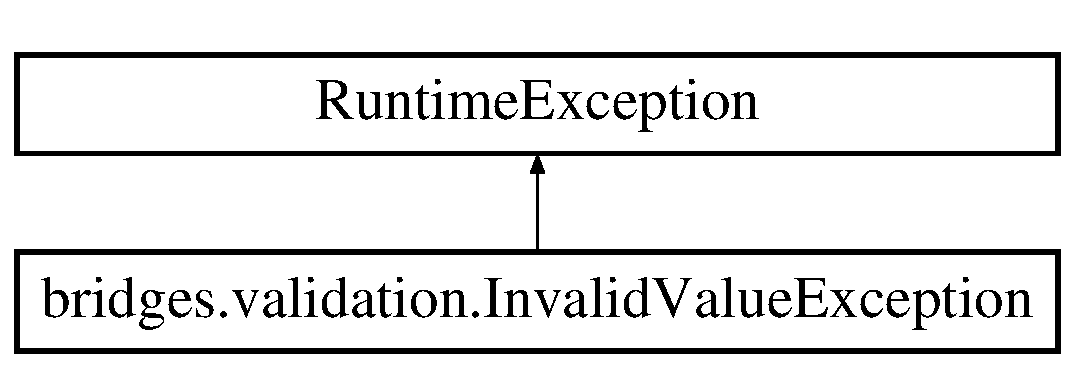
\includegraphics[height=2.000000cm]{classbridges_1_1validation_1_1_invalid_value_exception}
\end{center}
\end{figure}
\subsection*{Public Member Functions}
\begin{DoxyCompactItemize}
\item 
\mbox{\hyperlink{classbridges_1_1validation_1_1_invalid_value_exception_adf4c16bcef674454b87d8cc035efc75d}{Invalid\+Value\+Exception}} (String message)
\end{DoxyCompactItemize}


\subsection{Detailed Description}
Exception indicating invalid C\+SS values. Examples of uses for this include sizes with invalid units, and invalid colors. \begin{DoxyAuthor}{Author}
Sean Gallagher 
\end{DoxyAuthor}


\subsection{Constructor \& Destructor Documentation}
\mbox{\Hypertarget{classbridges_1_1validation_1_1_invalid_value_exception_adf4c16bcef674454b87d8cc035efc75d}\label{classbridges_1_1validation_1_1_invalid_value_exception_adf4c16bcef674454b87d8cc035efc75d}} 
\index{bridges\+::validation\+::\+Invalid\+Value\+Exception@{bridges\+::validation\+::\+Invalid\+Value\+Exception}!Invalid\+Value\+Exception@{Invalid\+Value\+Exception}}
\index{Invalid\+Value\+Exception@{Invalid\+Value\+Exception}!bridges\+::validation\+::\+Invalid\+Value\+Exception@{bridges\+::validation\+::\+Invalid\+Value\+Exception}}
\subsubsection{\texorpdfstring{Invalid\+Value\+Exception()}{InvalidValueException()}}
{\footnotesize\ttfamily bridges.\+validation.\+Invalid\+Value\+Exception.\+Invalid\+Value\+Exception (\begin{DoxyParamCaption}\item[{String}]{message }\end{DoxyParamCaption})}



The documentation for this class was generated from the following file\+:\begin{DoxyCompactItemize}
\item 
/\+Users/kalpathi/gr/bridges/client/java/bridges-\/17/src/main/java/bridges/validation/\mbox{\hyperlink{_invalid_value_exception_8java}{Invalid\+Value\+Exception.\+java}}\end{DoxyCompactItemize}

\hypertarget{classbridges_1_1base_1_1_link_visualizer}{}\section{bridges.\+base.\+Link\+Visualizer Class Reference}
\label{classbridges_1_1base_1_1_link_visualizer}\index{bridges.\+base.\+Link\+Visualizer@{bridges.\+base.\+Link\+Visualizer}}


This class maintains the visual attributes of links that join Bridges elements.  


\subsection*{Public Member Functions}
\begin{DoxyCompactItemize}
\item 
\hyperlink{classbridges_1_1base_1_1_link_visualizer_a0b69f099fa264ae9097b0efe278c6a1b}{Link\+Visualizer} ()
\item 
void \hyperlink{classbridges_1_1base_1_1_link_visualizer_a702e9ca345d1a4a035baf2041f275849}{set\+Thickness} (double th)
\item 
double \hyperlink{classbridges_1_1base_1_1_link_visualizer_af1592d2a8664b00c1a51fdc0f8d1860a}{get\+Thickness} ()
\item 
void \hyperlink{classbridges_1_1base_1_1_link_visualizer_a21d5884d243cf5a08f9d544f5083a44c}{set\+Weight} (double wt)
\item 
double \hyperlink{classbridges_1_1base_1_1_link_visualizer_ac96d7fb118ae6c7e1bdd57c5e2c8639a}{get\+Weight} ()
\item 
void \hyperlink{classbridges_1_1base_1_1_link_visualizer_a92f306dbd73b961befa8ab4c0620a89e}{set\+Color} (String col\+\_\+name)
\item 
void \hyperlink{classbridges_1_1base_1_1_link_visualizer_a003905cfe33e1704555b2b3a1cf99bad}{set\+Color} (Integer r, Integer g, Integer b, Float a)  throws Invalid\+Value\+Exception 
\item 
\hyperlink{classbridges_1_1base_1_1_color}{Color} \hyperlink{classbridges_1_1base_1_1_link_visualizer_a3ed52d98ecab99c6d8dd136fba913b7d}{get\+Color} ()
\item 
void \hyperlink{classbridges_1_1base_1_1_link_visualizer_ac0d59614dbc65ed0a19c25c493a1deaa}{set\+Opacity} (float opacity)
\item 
float \hyperlink{classbridges_1_1base_1_1_link_visualizer_a07cdd435a54e4b612ad63614f2a27a4a}{get\+Opacity} ()
\item 
String \hyperlink{classbridges_1_1base_1_1_link_visualizer_ab64d9b7e2b99f7ebce80cbabfe4adf2a}{get\+Link\+Properties} ()
\end{DoxyCompactItemize}


\subsection{Detailed Description}
This class maintains the visual attributes of links that join Bridges elements. 

Visual properties include color, thickness, and opacity. Objects of this class are stored as part of the \hyperlink{classbridges_1_1base_1_1_element}{Element} class. Generally, a user will manipulate the \hyperlink{classbridges_1_1base_1_1_link_visualizer}{Link\+Visualizer} returned from the \hyperlink{classbridges_1_1base_1_1_element}{Element}\textquotesingle{}s get\+Link\+Visualizer(\+Element it) method (which it is the Bridges element this element is linked to), and then set attributes using its methods. Links are utilized in all types of linked lists, tree and graph structures.

Supported attribute values are as follows\+:

{\bfseries Supported Colors (by name)}\+: 

\char`\"{}red\char`\"{}, \char`\"{}green\char`\"{}, \char`\"{}blue\char`\"{},\char`\"{}yellow\char`\"{},\char`\"{}cyan\char`\"{},\char`\"{}magenta\char`\"{}, \char`\"{}white\char`\"{},, \char`\"{}black\char`\"{}, \char`\"{}orange\char`\"{}, \char`\"{}turquoise\char`\"{}, \char`\"{}maroon\char`\"{}, ~\newline
 \char`\"{}aquamarine\char`\"{}, \char`\"{}azure\char`\"{}, \char`\"{}beige\char`\"{}, \char`\"{}brown\char`\"{}, \char`\"{}tan\char`\"{}, \char`\"{}olive\char`\"{}, \char`\"{}chartreuse\char`\"{}, \char`\"{}khaki\char`\"{}, \char`\"{}bisque\char`\"{}, \char`\"{}coral\char`\"{}, ~\newline
 \char`\"{}pink\char`\"{}, \char`\"{}lavender\char`\"{}, \char`\"{}purple\char`\"{}, \char`\"{}gold\char`\"{} 

{\bfseries  \hyperlink{classbridges_1_1base_1_1_color}{Color} by R\+G\+BA Specification \+:} Range\+: 0-\/255 for each component 

{\bfseries  Thickness\+: } Range \+: 0.\+0-\/50.\+0

{\bfseries  Opacity\+: } Range (0.\+0-\/1.\+0) 

\begin{DoxyAuthor}{Author}
Mihai Mehedint, Kalpathi Subramanian
\end{DoxyAuthor}
\begin{DoxyDate}{Date}
6/22/16, 1/16/17, 5/17/17
\end{DoxyDate}
\begin{DoxySeeAlso}{See also}
Example Tutorial at ~\newline
 \href{http://bridgesuncc.github.io/Hello_World_Tutorials/SLL.html}{\tt http\+://bridgesuncc.\+github.\+io/\+Hello\+\_\+\+World\+\_\+\+Tutorials/\+S\+L\+L.\+html} 
\end{DoxySeeAlso}


\subsection{Constructor \& Destructor Documentation}
\hypertarget{classbridges_1_1base_1_1_link_visualizer_a0b69f099fa264ae9097b0efe278c6a1b}{}\label{classbridges_1_1base_1_1_link_visualizer_a0b69f099fa264ae9097b0efe278c6a1b} 
\index{bridges\+::base\+::\+Link\+Visualizer@{bridges\+::base\+::\+Link\+Visualizer}!Link\+Visualizer@{Link\+Visualizer}}
\index{Link\+Visualizer@{Link\+Visualizer}!bridges\+::base\+::\+Link\+Visualizer@{bridges\+::base\+::\+Link\+Visualizer}}
\subsubsection{\texorpdfstring{Link\+Visualizer()}{LinkVisualizer()}}
{\footnotesize\ttfamily bridges.\+base.\+Link\+Visualizer.\+Link\+Visualizer (\begin{DoxyParamCaption}{ }\end{DoxyParamCaption})}



\subsection{Member Function Documentation}
\hypertarget{classbridges_1_1base_1_1_link_visualizer_a3ed52d98ecab99c6d8dd136fba913b7d}{}\label{classbridges_1_1base_1_1_link_visualizer_a3ed52d98ecab99c6d8dd136fba913b7d} 
\index{bridges\+::base\+::\+Link\+Visualizer@{bridges\+::base\+::\+Link\+Visualizer}!get\+Color@{get\+Color}}
\index{get\+Color@{get\+Color}!bridges\+::base\+::\+Link\+Visualizer@{bridges\+::base\+::\+Link\+Visualizer}}
\subsubsection{\texorpdfstring{get\+Color()}{getColor()}}
{\footnotesize\ttfamily \hyperlink{classbridges_1_1base_1_1_color}{Color} bridges.\+base.\+Link\+Visualizer.\+get\+Color (\begin{DoxyParamCaption}{ }\end{DoxyParamCaption})}

Get the color of the link in the Bridges Visualization

\begin{DoxyReturn}{Returns}
the \hyperlink{classbridges_1_1base_1_1_color}{Color} object representing the color of the link 
\end{DoxyReturn}
\hypertarget{classbridges_1_1base_1_1_link_visualizer_ab64d9b7e2b99f7ebce80cbabfe4adf2a}{}\label{classbridges_1_1base_1_1_link_visualizer_ab64d9b7e2b99f7ebce80cbabfe4adf2a} 
\index{bridges\+::base\+::\+Link\+Visualizer@{bridges\+::base\+::\+Link\+Visualizer}!get\+Link\+Properties@{get\+Link\+Properties}}
\index{get\+Link\+Properties@{get\+Link\+Properties}!bridges\+::base\+::\+Link\+Visualizer@{bridges\+::base\+::\+Link\+Visualizer}}
\subsubsection{\texorpdfstring{get\+Link\+Properties()}{getLinkProperties()}}
{\footnotesize\ttfamily String bridges.\+base.\+Link\+Visualizer.\+get\+Link\+Properties (\begin{DoxyParamCaption}{ }\end{DoxyParamCaption})}

\hypertarget{classbridges_1_1base_1_1_link_visualizer_a07cdd435a54e4b612ad63614f2a27a4a}{}\label{classbridges_1_1base_1_1_link_visualizer_a07cdd435a54e4b612ad63614f2a27a4a} 
\index{bridges\+::base\+::\+Link\+Visualizer@{bridges\+::base\+::\+Link\+Visualizer}!get\+Opacity@{get\+Opacity}}
\index{get\+Opacity@{get\+Opacity}!bridges\+::base\+::\+Link\+Visualizer@{bridges\+::base\+::\+Link\+Visualizer}}
\subsubsection{\texorpdfstring{get\+Opacity()}{getOpacity()}}
{\footnotesize\ttfamily float bridges.\+base.\+Link\+Visualizer.\+get\+Opacity (\begin{DoxyParamCaption}{ }\end{DoxyParamCaption})}

Get the opacity of the link in the Bridges Visualization

\begin{DoxyReturn}{Returns}
the opacity value (in the range 0.\+0-\/1.\+0 
\end{DoxyReturn}
\hypertarget{classbridges_1_1base_1_1_link_visualizer_af1592d2a8664b00c1a51fdc0f8d1860a}{}\label{classbridges_1_1base_1_1_link_visualizer_af1592d2a8664b00c1a51fdc0f8d1860a} 
\index{bridges\+::base\+::\+Link\+Visualizer@{bridges\+::base\+::\+Link\+Visualizer}!get\+Thickness@{get\+Thickness}}
\index{get\+Thickness@{get\+Thickness}!bridges\+::base\+::\+Link\+Visualizer@{bridges\+::base\+::\+Link\+Visualizer}}
\subsubsection{\texorpdfstring{get\+Thickness()}{getThickness()}}
{\footnotesize\ttfamily double bridges.\+base.\+Link\+Visualizer.\+get\+Thickness (\begin{DoxyParamCaption}{ }\end{DoxyParamCaption})}

Get the thickness of the link in the Bridges Visualiation

\begin{DoxyReturn}{Returns}
the size in pixels of the \hyperlink{classbridges_1_1base_1_1_element}{Element} in the Bridges Visualization 
\end{DoxyReturn}
\hypertarget{classbridges_1_1base_1_1_link_visualizer_ac96d7fb118ae6c7e1bdd57c5e2c8639a}{}\label{classbridges_1_1base_1_1_link_visualizer_ac96d7fb118ae6c7e1bdd57c5e2c8639a} 
\index{bridges\+::base\+::\+Link\+Visualizer@{bridges\+::base\+::\+Link\+Visualizer}!get\+Weight@{get\+Weight}}
\index{get\+Weight@{get\+Weight}!bridges\+::base\+::\+Link\+Visualizer@{bridges\+::base\+::\+Link\+Visualizer}}
\subsubsection{\texorpdfstring{get\+Weight()}{getWeight()}}
{\footnotesize\ttfamily double bridges.\+base.\+Link\+Visualizer.\+get\+Weight (\begin{DoxyParamCaption}{ }\end{DoxyParamCaption})}

Get the weight of the link

\begin{DoxyReturn}{Returns}
the stored edge weight 
\end{DoxyReturn}
\hypertarget{classbridges_1_1base_1_1_link_visualizer_a92f306dbd73b961befa8ab4c0620a89e}{}\label{classbridges_1_1base_1_1_link_visualizer_a92f306dbd73b961befa8ab4c0620a89e} 
\index{bridges\+::base\+::\+Link\+Visualizer@{bridges\+::base\+::\+Link\+Visualizer}!set\+Color@{set\+Color}}
\index{set\+Color@{set\+Color}!bridges\+::base\+::\+Link\+Visualizer@{bridges\+::base\+::\+Link\+Visualizer}}
\subsubsection{\texorpdfstring{set\+Color()}{setColor()}\hspace{0.1cm}{\footnotesize\ttfamily [1/2]}}
{\footnotesize\ttfamily void bridges.\+base.\+Link\+Visualizer.\+set\+Color (\begin{DoxyParamCaption}\item[{String}]{col\+\_\+name }\end{DoxyParamCaption})}

Set the color of the link in the Bridges Visualization to \char`\"{}a\+Color\char`\"{}.


\begin{DoxyParams}{Parameters}
{\em col\+\_\+name} & the string reprsenting the color of the \hyperlink{classbridges_1_1base_1_1_element}{Element} in the Bridges Visualization; supported named colors are \char`\"{}red\char`\"{}, \char`\"{}green\char`\"{}, \char`\"{}blue\char`\"{}, \char`\"{}yellow\char`\"{}, \char`\"{}cyan\char`\"{}, \char`\"{}magenta\char`\"{}, \char`\"{}white\char`\"{}, \char`\"{}black\char`\"{}, \char`\"{}orange\char`\"{}, \char`\"{}turquoise\char`\"{}, \char`\"{}maroon\char`\"{}, \char`\"{}aquamarine\char`\"{}, \char`\"{}azure\char`\"{}, \char`\"{}beige\char`\"{}, \char`\"{}brown\char`\"{}, \char`\"{}tan\char`\"{}, \char`\"{}olive\char`\"{}, \char`\"{}chartreuse\char`\"{}, \char`\"{}khaki\char`\"{}, \char`\"{}bisque\char`\"{}, \char`\"{}coral\char`\"{}, \char`\"{}pink\char`\"{}, \char`\"{}lavender\char`\"{}, \char`\"{}purple\char`\"{}, \char`\"{}gold\char`\"{} \\
\hline
\end{DoxyParams}
\hypertarget{classbridges_1_1base_1_1_link_visualizer_a003905cfe33e1704555b2b3a1cf99bad}{}\label{classbridges_1_1base_1_1_link_visualizer_a003905cfe33e1704555b2b3a1cf99bad} 
\index{bridges\+::base\+::\+Link\+Visualizer@{bridges\+::base\+::\+Link\+Visualizer}!set\+Color@{set\+Color}}
\index{set\+Color@{set\+Color}!bridges\+::base\+::\+Link\+Visualizer@{bridges\+::base\+::\+Link\+Visualizer}}
\subsubsection{\texorpdfstring{set\+Color()}{setColor()}\hspace{0.1cm}{\footnotesize\ttfamily [2/2]}}
{\footnotesize\ttfamily void bridges.\+base.\+Link\+Visualizer.\+set\+Color (\begin{DoxyParamCaption}\item[{Integer}]{r,  }\item[{Integer}]{g,  }\item[{Integer}]{b,  }\item[{Float}]{a }\end{DoxyParamCaption}) throws \hyperlink{classbridges_1_1validation_1_1_invalid_value_exception}{Invalid\+Value\+Exception}}

Set the color of the link given R\+G\+BA components


\begin{DoxyParams}{Parameters}
{\em r,g,b,a} & components\\
\hline
\end{DoxyParams}
check to ensure they are in 0-\/255 range, else throw exception \hypertarget{classbridges_1_1base_1_1_link_visualizer_ac0d59614dbc65ed0a19c25c493a1deaa}{}\label{classbridges_1_1base_1_1_link_visualizer_ac0d59614dbc65ed0a19c25c493a1deaa} 
\index{bridges\+::base\+::\+Link\+Visualizer@{bridges\+::base\+::\+Link\+Visualizer}!set\+Opacity@{set\+Opacity}}
\index{set\+Opacity@{set\+Opacity}!bridges\+::base\+::\+Link\+Visualizer@{bridges\+::base\+::\+Link\+Visualizer}}
\subsubsection{\texorpdfstring{set\+Opacity()}{setOpacity()}}
{\footnotesize\ttfamily void bridges.\+base.\+Link\+Visualizer.\+set\+Opacity (\begin{DoxyParamCaption}\item[{float}]{opacity }\end{DoxyParamCaption})}

Sets the opacity of the link in the Bridges Visualization


\begin{DoxyParams}{Parameters}
{\em opacity} & a float between 0 and 1 representing how transparent the node should be on the Bridges Visualization. 0 for invisible, 1 for fully visible, a decimal between 0 and 1 for varying transparency. \\
\hline
\end{DoxyParams}
\hypertarget{classbridges_1_1base_1_1_link_visualizer_a702e9ca345d1a4a035baf2041f275849}{}\label{classbridges_1_1base_1_1_link_visualizer_a702e9ca345d1a4a035baf2041f275849} 
\index{bridges\+::base\+::\+Link\+Visualizer@{bridges\+::base\+::\+Link\+Visualizer}!set\+Thickness@{set\+Thickness}}
\index{set\+Thickness@{set\+Thickness}!bridges\+::base\+::\+Link\+Visualizer@{bridges\+::base\+::\+Link\+Visualizer}}
\subsubsection{\texorpdfstring{set\+Thickness()}{setThickness()}}
{\footnotesize\ttfamily void bridges.\+base.\+Link\+Visualizer.\+set\+Thickness (\begin{DoxyParamCaption}\item[{double}]{th }\end{DoxyParamCaption})}

Set the thickness of the link in the Bridge Visualization in pixels; thickness shoudl be in the range 0-\/50.\+0


\begin{DoxyParams}{Parameters}
{\em thickness} & \\
\hline
\end{DoxyParams}
\hypertarget{classbridges_1_1base_1_1_link_visualizer_a21d5884d243cf5a08f9d544f5083a44c}{}\label{classbridges_1_1base_1_1_link_visualizer_a21d5884d243cf5a08f9d544f5083a44c} 
\index{bridges\+::base\+::\+Link\+Visualizer@{bridges\+::base\+::\+Link\+Visualizer}!set\+Weight@{set\+Weight}}
\index{set\+Weight@{set\+Weight}!bridges\+::base\+::\+Link\+Visualizer@{bridges\+::base\+::\+Link\+Visualizer}}
\subsubsection{\texorpdfstring{set\+Weight()}{setWeight()}}
{\footnotesize\ttfamily void bridges.\+base.\+Link\+Visualizer.\+set\+Weight (\begin{DoxyParamCaption}\item[{double}]{wt }\end{DoxyParamCaption})}

Set the weight of the link, useful in graph algorithms, for example. weight value is user defined, and determined by the input graph specification.


\begin{DoxyParams}{Parameters}
{\em weight} & \\
\hline
\end{DoxyParams}


The documentation for this class was generated from the following file\+:\begin{DoxyCompactItemize}
\item 
link/base/\hyperlink{_link_visualizer_8java}{Link\+Visualizer.\+java}\end{DoxyCompactItemize}

\hypertarget{classbridges_1_1base_1_1_m_lelement}{}\doxysection{bridges.\+base.\+M\+Lelement$<$ E $>$ Class Template Reference}
\label{classbridges_1_1base_1_1_m_lelement}\index{bridges.base.MLelement$<$ E $>$@{bridges.base.MLelement$<$ E $>$}}
Inheritance diagram for bridges.\+base.\+M\+Lelement$<$ E $>$\+:\begin{figure}[H]
\begin{center}
\leavevmode
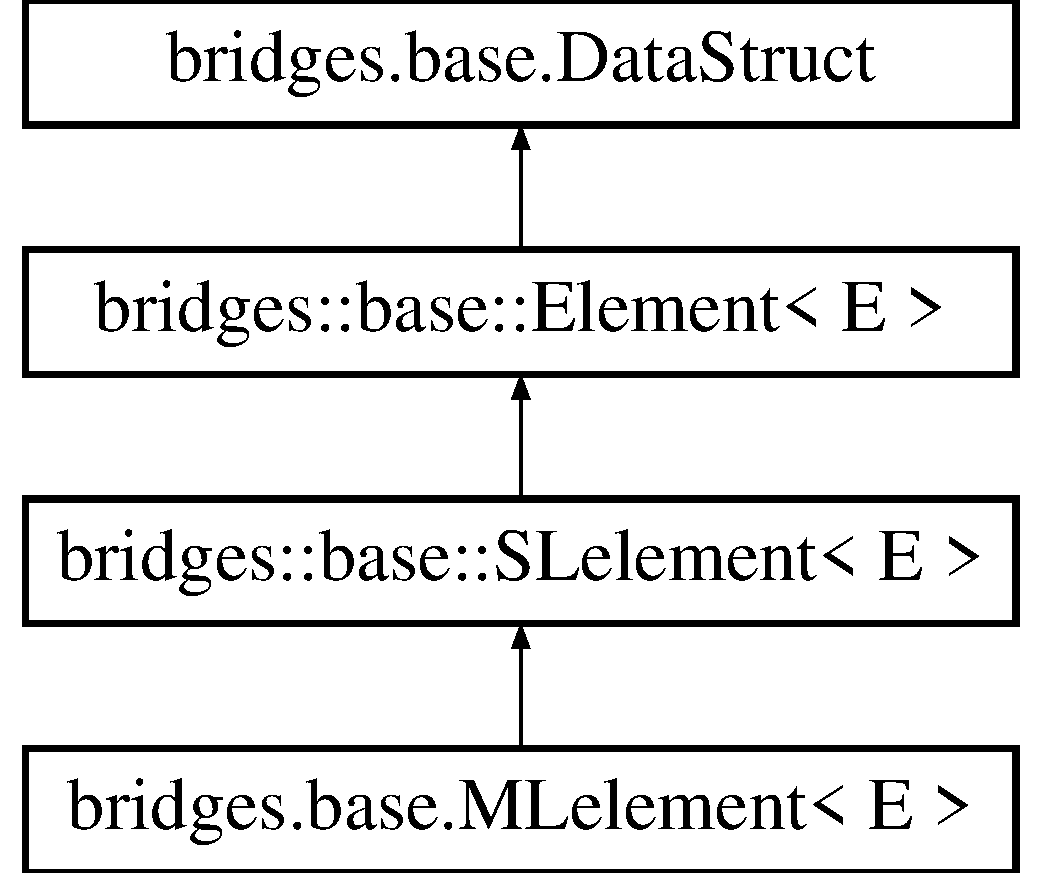
\includegraphics[height=4.000000cm]{classbridges_1_1base_1_1_m_lelement}
\end{center}
\end{figure}


\doxysubsection{Detailed Description}
\begin{DoxyVerb}@brief This class can be used to instantiate Multi-list Elements.
\end{DoxyVerb}


This class extends \mbox{\hyperlink{classbridges_1_1base_1_1_s_lelement}{S\+Lelement}} (singly linked list element) to build multi-\/lists; Multilist elements contain a tag (boolean) that indicates if the element contains a sublist or not; if the tag is true, then there is a sublist beginning at this node and the starting point is the `sublist' field in the element. If the tag is false, then the list continues as a normal singly linked list. The sublists are re recursive\+: any sublist can have its own sublists and so on.

As in singly linked elements, the next pointer points to the following list element and each element contains a generic application specific object. This class extends \mbox{\hyperlink{classbridges_1_1base_1_1_s_lelement}{S\+Lelement}} (singly linked list element) to build multi-\/lists; Multilist elements contain a tag that indicates if the element is a sublist or not; If the element points to a sublist, then the sublist field is the beginning of this sublist. If not, the data field contains the user specified data item and list continues (\mbox{\hyperlink{classbridges_1_1base_1_1_m_lelement_a52ddc26a69eccda5f5b57b94cf87a545}{get\+Next()}}/set\+Next()). As in singly linked elements, the next pointer points to the following list element of the list or sublist. \begin{DoxyVerb}Multi-list elements contain a visualizer (ElementVisualizer) object for setting
\end{DoxyVerb}
 visual attributes (color, shape, opacity, size), necessary for displaying them in a web browser.

Elements also have a \mbox{\hyperlink{classbridges_1_1base_1_1_link_visualizer}{Link\+Visualizer}} object, that is used when they are linked to another element, appropriate for setting link attributes, for instance, between the current element and its next element. In this case, the link in question is that which connects the element to the following elements; a similar logic follows for sublists.

\begin{DoxySeeAlso}{See also}
Example Tutorial at \href{http://bridgesuncc.github.io/tutorials/MultiList.html}{\texttt{ http\+://bridgesuncc.\+github.\+io/tutorials/\+Multi\+List.\+html}}
\end{DoxySeeAlso}
\begin{DoxyAuthor}{Author}
Kalpathi Subramanian
\end{DoxyAuthor}
\begin{DoxyDate}{Date}
5/24/17, 7/14/19
\end{DoxyDate}

\begin{DoxyParams}{Parameters}
{\em E} & The generic parameter object that is part of this element, representing either application specific data, or a pointer to a sublist. \\
\hline
\end{DoxyParams}
\doxysubsection*{Public Member Functions}
\begin{DoxyCompactItemize}
\item 
\mbox{\hyperlink{classbridges_1_1base_1_1_m_lelement_a721d1369c297dc3a3617a1476cb6f5f8}{M\+Lelement}} ()
\item 
\mbox{\hyperlink{classbridges_1_1base_1_1_m_lelement_ad0437d26107039d98cdba6277cff19e2}{M\+Lelement}} (String label, E e)
\item 
\mbox{\hyperlink{classbridges_1_1base_1_1_m_lelement_ad3d5fe59028cd6854eb2abceefad7f7d}{M\+Lelement}} (E e, \mbox{\hyperlink{classbridges_1_1base_1_1_m_lelement}{M\+Lelement}}$<$ E $>$ \mbox{\hyperlink{classbridges_1_1base_1_1_s_lelement_abf61c96a74ad319d561c6952ea388e0e}{next}})
\item 
\mbox{\hyperlink{classbridges_1_1base_1_1_m_lelement_aa660281523a7de140a0b17737096a332}{M\+Lelement}} (\mbox{\hyperlink{classbridges_1_1base_1_1_m_lelement}{M\+Lelement}}$<$ E $>$ sublist, \mbox{\hyperlink{classbridges_1_1base_1_1_m_lelement}{M\+Lelement}}$<$ E $>$ \mbox{\hyperlink{classbridges_1_1base_1_1_s_lelement_abf61c96a74ad319d561c6952ea388e0e}{next}})
\item 
void \mbox{\hyperlink{classbridges_1_1base_1_1_m_lelement_ab13a42b947edc61106ea56c8bd4e78fc}{set\+Sub\+List}} (\mbox{\hyperlink{classbridges_1_1base_1_1_m_lelement}{M\+Lelement}}$<$ E $>$ sl)
\item 
\mbox{\hyperlink{classbridges_1_1base_1_1_m_lelement}{M\+Lelement}} \mbox{\hyperlink{classbridges_1_1base_1_1_m_lelement_afd44cb6e17e16e13a80190747c3b7994}{get\+Sub\+List}} ()
\item 
String \mbox{\hyperlink{classbridges_1_1base_1_1_m_lelement_aa2e26697e2c70a36b8345a324d00679a}{get\+Data\+Struct\+Type}} ()
\item 
\mbox{\hyperlink{classbridges_1_1base_1_1_m_lelement}{M\+Lelement}}$<$ E $>$ \mbox{\hyperlink{classbridges_1_1base_1_1_m_lelement_a52ddc26a69eccda5f5b57b94cf87a545}{get\+Next}} ()
\item 
void \mbox{\hyperlink{classbridges_1_1base_1_1_m_lelement_a60a431ce1b27c98219924075ea764ced}{set\+Tag}} (boolean t)
\item 
boolean \mbox{\hyperlink{classbridges_1_1base_1_1_m_lelement_a95dd0972a3a47cc8ed361cf50508eaa1}{get\+Tag}} ()
\item 
String \mbox{\hyperlink{classbridges_1_1base_1_1_m_lelement_a392f05256ac08e9c19ded1387ebb7583}{get\+Data\+Structure\+Representation}} ()
\end{DoxyCompactItemize}
\doxysubsection*{Protected Member Functions}
\begin{DoxyCompactItemize}
\item 
void \mbox{\hyperlink{classbridges_1_1base_1_1_m_lelement_a496378739f031ef451a6ab1f63c5770f}{get\+List\+Elements}} (Vector$<$ \mbox{\hyperlink{classbridges_1_1base_1_1_element}{Element}}$<$ E $>$$>$ nodes)
\end{DoxyCompactItemize}
\doxysubsection*{Protected Attributes}
\begin{DoxyCompactItemize}
\item 
\mbox{\hyperlink{classbridges_1_1base_1_1_m_lelement}{M\+Lelement}}$<$ E $>$ \mbox{\hyperlink{classbridges_1_1base_1_1_m_lelement_a7dee2985f9a8134d3076eb9478422403}{sub\+\_\+list}} = null
\end{DoxyCompactItemize}


\doxysubsection{Constructor \& Destructor Documentation}
\mbox{\Hypertarget{classbridges_1_1base_1_1_m_lelement_a721d1369c297dc3a3617a1476cb6f5f8}\label{classbridges_1_1base_1_1_m_lelement_a721d1369c297dc3a3617a1476cb6f5f8}} 
\index{bridges.base.MLelement$<$ E $>$@{bridges.base.MLelement$<$ E $>$}!MLelement@{MLelement}}
\index{MLelement@{MLelement}!bridges.base.MLelement$<$ E $>$@{bridges.base.MLelement$<$ E $>$}}
\doxysubsubsection{\texorpdfstring{MLelement()}{MLelement()}\hspace{0.1cm}{\footnotesize\ttfamily [1/4]}}
{\footnotesize\ttfamily \mbox{\hyperlink{classbridges_1_1base_1_1_m_lelement}{bridges.\+base.\+M\+Lelement}}$<$ E $>$.\mbox{\hyperlink{classbridges_1_1base_1_1_m_lelement}{M\+Lelement}} (\begin{DoxyParamCaption}{ }\end{DoxyParamCaption})}

This constructor creates an \mbox{\hyperlink{classbridges_1_1base_1_1_m_lelement}{M\+Lelement}} object and sets the next pointer to null \mbox{\Hypertarget{classbridges_1_1base_1_1_m_lelement_ad0437d26107039d98cdba6277cff19e2}\label{classbridges_1_1base_1_1_m_lelement_ad0437d26107039d98cdba6277cff19e2}} 
\index{bridges.base.MLelement$<$ E $>$@{bridges.base.MLelement$<$ E $>$}!MLelement@{MLelement}}
\index{MLelement@{MLelement}!bridges.base.MLelement$<$ E $>$@{bridges.base.MLelement$<$ E $>$}}
\doxysubsubsection{\texorpdfstring{MLelement()}{MLelement()}\hspace{0.1cm}{\footnotesize\ttfamily [2/4]}}
{\footnotesize\ttfamily \mbox{\hyperlink{classbridges_1_1base_1_1_m_lelement}{bridges.\+base.\+M\+Lelement}}$<$ E $>$.\mbox{\hyperlink{classbridges_1_1base_1_1_m_lelement}{M\+Lelement}} (\begin{DoxyParamCaption}\item[{String}]{label,  }\item[{E}]{e }\end{DoxyParamCaption})}

This constructor creates an \mbox{\hyperlink{classbridges_1_1base_1_1_m_lelement}{M\+Lelement}} object of generic parameter object E, and label \char`\"{}label\char`\"{} and sets the next pointer to null


\begin{DoxyParams}{Parameters}
{\em label} & the label of \mbox{\hyperlink{classbridges_1_1base_1_1_m_lelement}{M\+Lelement}} that shows up on the Bridges visualization \\
\hline
{\em e} & the generic object that this \mbox{\hyperlink{classbridges_1_1base_1_1_m_lelement}{M\+Lelement}} will hold \\
\hline
\end{DoxyParams}
\mbox{\Hypertarget{classbridges_1_1base_1_1_m_lelement_ad3d5fe59028cd6854eb2abceefad7f7d}\label{classbridges_1_1base_1_1_m_lelement_ad3d5fe59028cd6854eb2abceefad7f7d}} 
\index{bridges.base.MLelement$<$ E $>$@{bridges.base.MLelement$<$ E $>$}!MLelement@{MLelement}}
\index{MLelement@{MLelement}!bridges.base.MLelement$<$ E $>$@{bridges.base.MLelement$<$ E $>$}}
\doxysubsubsection{\texorpdfstring{MLelement()}{MLelement()}\hspace{0.1cm}{\footnotesize\ttfamily [3/4]}}
{\footnotesize\ttfamily \mbox{\hyperlink{classbridges_1_1base_1_1_m_lelement}{bridges.\+base.\+M\+Lelement}}$<$ E $>$.\mbox{\hyperlink{classbridges_1_1base_1_1_m_lelement}{M\+Lelement}} (\begin{DoxyParamCaption}\item[{E}]{e,  }\item[{\mbox{\hyperlink{classbridges_1_1base_1_1_m_lelement}{M\+Lelement}}$<$ E $>$}]{next }\end{DoxyParamCaption})}

Creates a new element with value \char`\"{}e\char`\"{} and sets the next pointer to the \mbox{\hyperlink{classbridges_1_1base_1_1_m_lelement}{M\+Lelement}} referenced by the \char`\"{}next\char`\"{} argument


\begin{DoxyParams}{Parameters}
{\em e} & the generic object that this element will hold \\
\hline
{\em next} & the element that should be assigned to the next pointer \\
\hline
\end{DoxyParams}
\mbox{\Hypertarget{classbridges_1_1base_1_1_m_lelement_aa660281523a7de140a0b17737096a332}\label{classbridges_1_1base_1_1_m_lelement_aa660281523a7de140a0b17737096a332}} 
\index{bridges.base.MLelement$<$ E $>$@{bridges.base.MLelement$<$ E $>$}!MLelement@{MLelement}}
\index{MLelement@{MLelement}!bridges.base.MLelement$<$ E $>$@{bridges.base.MLelement$<$ E $>$}}
\doxysubsubsection{\texorpdfstring{MLelement()}{MLelement()}\hspace{0.1cm}{\footnotesize\ttfamily [4/4]}}
{\footnotesize\ttfamily \mbox{\hyperlink{classbridges_1_1base_1_1_m_lelement}{bridges.\+base.\+M\+Lelement}}$<$ E $>$.\mbox{\hyperlink{classbridges_1_1base_1_1_m_lelement}{M\+Lelement}} (\begin{DoxyParamCaption}\item[{\mbox{\hyperlink{classbridges_1_1base_1_1_m_lelement}{M\+Lelement}}$<$ E $>$}]{sublist,  }\item[{\mbox{\hyperlink{classbridges_1_1base_1_1_m_lelement}{M\+Lelement}}$<$ E $>$}]{next }\end{DoxyParamCaption})}

Creates a new element and sets the next pointer to the \mbox{\hyperlink{classbridges_1_1base_1_1_m_lelement}{M\+Lelement}} \char`\"{}next\char`\"{} 
\begin{DoxyParams}{Parameters}
{\em next} & the \mbox{\hyperlink{classbridges_1_1base_1_1_m_lelement}{M\+Lelement}} that should be assigned to the next pointer \\
\hline
\end{DoxyParams}


\doxysubsection{Member Function Documentation}
\mbox{\Hypertarget{classbridges_1_1base_1_1_m_lelement_aa2e26697e2c70a36b8345a324d00679a}\label{classbridges_1_1base_1_1_m_lelement_aa2e26697e2c70a36b8345a324d00679a}} 
\index{bridges.base.MLelement$<$ E $>$@{bridges.base.MLelement$<$ E $>$}!getDataStructType@{getDataStructType}}
\index{getDataStructType@{getDataStructType}!bridges.base.MLelement$<$ E $>$@{bridges.base.MLelement$<$ E $>$}}
\doxysubsubsection{\texorpdfstring{getDataStructType()}{getDataStructType()}}
{\footnotesize\ttfamily String \mbox{\hyperlink{classbridges_1_1base_1_1_m_lelement}{bridges.\+base.\+M\+Lelement}}$<$ E $>$.get\+Data\+Struct\+Type (\begin{DoxyParamCaption}{ }\end{DoxyParamCaption})}

This method gets the data structure type

\begin{DoxyReturn}{Returns}
The date structure type as a string 
\end{DoxyReturn}


Reimplemented from \mbox{\hyperlink{classbridges_1_1base_1_1_s_lelement_a8c48a2d34b238fa0ae7bf2d1ee58ea88}{bridges.\+base.\+S\+Lelement$<$ E $>$}}.

\mbox{\Hypertarget{classbridges_1_1base_1_1_m_lelement_a392f05256ac08e9c19ded1387ebb7583}\label{classbridges_1_1base_1_1_m_lelement_a392f05256ac08e9c19ded1387ebb7583}} 
\index{bridges.base.MLelement$<$ E $>$@{bridges.base.MLelement$<$ E $>$}!getDataStructureRepresentation@{getDataStructureRepresentation}}
\index{getDataStructureRepresentation@{getDataStructureRepresentation}!bridges.base.MLelement$<$ E $>$@{bridges.base.MLelement$<$ E $>$}}
\doxysubsubsection{\texorpdfstring{getDataStructureRepresentation()}{getDataStructureRepresentation()}}
{\footnotesize\ttfamily String \mbox{\hyperlink{classbridges_1_1base_1_1_m_lelement}{bridges.\+base.\+M\+Lelement}}$<$ E $>$.get\+Data\+Structure\+Representation (\begin{DoxyParamCaption}{ }\end{DoxyParamCaption})}

Get the J\+S\+ON representation of the the data structure

\begin{DoxyReturn}{Returns}
the J\+S\+ON string of the element\textquotesingle{}s representation 
\end{DoxyReturn}


Reimplemented from \mbox{\hyperlink{classbridges_1_1base_1_1_s_lelement_a2928f5e8640deaceeecf01adcd75669b}{bridges.\+base.\+S\+Lelement$<$ E $>$}}.

\mbox{\Hypertarget{classbridges_1_1base_1_1_m_lelement_a496378739f031ef451a6ab1f63c5770f}\label{classbridges_1_1base_1_1_m_lelement_a496378739f031ef451a6ab1f63c5770f}} 
\index{bridges.base.MLelement$<$ E $>$@{bridges.base.MLelement$<$ E $>$}!getListElements@{getListElements}}
\index{getListElements@{getListElements}!bridges.base.MLelement$<$ E $>$@{bridges.base.MLelement$<$ E $>$}}
\doxysubsubsection{\texorpdfstring{getListElements()}{getListElements()}}
{\footnotesize\ttfamily void \mbox{\hyperlink{classbridges_1_1base_1_1_m_lelement}{bridges.\+base.\+M\+Lelement}}$<$ E $>$.get\+List\+Elements (\begin{DoxyParamCaption}\item[{Vector$<$ \mbox{\hyperlink{classbridges_1_1base_1_1_element}{Element}}$<$ E $>$$>$}]{nodes }\end{DoxyParamCaption})\hspace{0.3cm}{\ttfamily [protected]}}



Reimplemented from \mbox{\hyperlink{classbridges_1_1base_1_1_s_lelement_abadffea339171349a8e86ded9cd3fe21}{bridges.\+base.\+S\+Lelement$<$ E $>$}}.

\mbox{\Hypertarget{classbridges_1_1base_1_1_m_lelement_a52ddc26a69eccda5f5b57b94cf87a545}\label{classbridges_1_1base_1_1_m_lelement_a52ddc26a69eccda5f5b57b94cf87a545}} 
\index{bridges.base.MLelement$<$ E $>$@{bridges.base.MLelement$<$ E $>$}!getNext@{getNext}}
\index{getNext@{getNext}!bridges.base.MLelement$<$ E $>$@{bridges.base.MLelement$<$ E $>$}}
\doxysubsubsection{\texorpdfstring{getNext()}{getNext()}}
{\footnotesize\ttfamily \mbox{\hyperlink{classbridges_1_1base_1_1_m_lelement}{M\+Lelement}}$<$E$>$ \mbox{\hyperlink{classbridges_1_1base_1_1_m_lelement}{bridges.\+base.\+M\+Lelement}}$<$ E $>$.get\+Next (\begin{DoxyParamCaption}{ }\end{DoxyParamCaption})}

Retrieves the element following this element

\begin{DoxyReturn}{Returns}
M\+Lelement$<$\+E$>$ assigned to next 
\end{DoxyReturn}


Reimplemented from \mbox{\hyperlink{classbridges_1_1base_1_1_s_lelement_a060c4671e05e3f20b16630343393b80d}{bridges.\+base.\+S\+Lelement$<$ E $>$}}.

\mbox{\Hypertarget{classbridges_1_1base_1_1_m_lelement_afd44cb6e17e16e13a80190747c3b7994}\label{classbridges_1_1base_1_1_m_lelement_afd44cb6e17e16e13a80190747c3b7994}} 
\index{bridges.base.MLelement$<$ E $>$@{bridges.base.MLelement$<$ E $>$}!getSubList@{getSubList}}
\index{getSubList@{getSubList}!bridges.base.MLelement$<$ E $>$@{bridges.base.MLelement$<$ E $>$}}
\doxysubsubsection{\texorpdfstring{getSubList()}{getSubList()}}
{\footnotesize\ttfamily \mbox{\hyperlink{classbridges_1_1base_1_1_m_lelement}{M\+Lelement}} \mbox{\hyperlink{classbridges_1_1base_1_1_m_lelement}{bridges.\+base.\+M\+Lelement}}$<$ E $>$.get\+Sub\+List (\begin{DoxyParamCaption}{ }\end{DoxyParamCaption})}

Gets the sublist at this node, if it exists

\begin{DoxyReturn}{Returns}
the sublist head element, if it exists 
\end{DoxyReturn}
\mbox{\Hypertarget{classbridges_1_1base_1_1_m_lelement_a95dd0972a3a47cc8ed361cf50508eaa1}\label{classbridges_1_1base_1_1_m_lelement_a95dd0972a3a47cc8ed361cf50508eaa1}} 
\index{bridges.base.MLelement$<$ E $>$@{bridges.base.MLelement$<$ E $>$}!getTag@{getTag}}
\index{getTag@{getTag}!bridges.base.MLelement$<$ E $>$@{bridges.base.MLelement$<$ E $>$}}
\doxysubsubsection{\texorpdfstring{getTag()}{getTag()}}
{\footnotesize\ttfamily boolean \mbox{\hyperlink{classbridges_1_1base_1_1_m_lelement}{bridges.\+base.\+M\+Lelement}}$<$ E $>$.get\+Tag (\begin{DoxyParamCaption}{ }\end{DoxyParamCaption})}

Gets the tag of the element.

\begin{DoxyReturn}{Returns}
tag of the element 
\end{DoxyReturn}
\mbox{\Hypertarget{classbridges_1_1base_1_1_m_lelement_ab13a42b947edc61106ea56c8bd4e78fc}\label{classbridges_1_1base_1_1_m_lelement_ab13a42b947edc61106ea56c8bd4e78fc}} 
\index{bridges.base.MLelement$<$ E $>$@{bridges.base.MLelement$<$ E $>$}!setSubList@{setSubList}}
\index{setSubList@{setSubList}!bridges.base.MLelement$<$ E $>$@{bridges.base.MLelement$<$ E $>$}}
\doxysubsubsection{\texorpdfstring{setSubList()}{setSubList()}}
{\footnotesize\ttfamily void \mbox{\hyperlink{classbridges_1_1base_1_1_m_lelement}{bridges.\+base.\+M\+Lelement}}$<$ E $>$.set\+Sub\+List (\begin{DoxyParamCaption}\item[{\mbox{\hyperlink{classbridges_1_1base_1_1_m_lelement}{M\+Lelement}}$<$ E $>$}]{sl }\end{DoxyParamCaption})}

Sets the start of a new sublist. to the \mbox{\hyperlink{classbridges_1_1base_1_1_m_lelement}{M\+Lelement}} \char`\"{}next\char`\"{}


\begin{DoxyParams}{Parameters}
{\em sl} & the \mbox{\hyperlink{classbridges_1_1base_1_1_m_lelement}{M\+Lelement}} that is the beginning of a sublist \\
\hline
\end{DoxyParams}
\mbox{\Hypertarget{classbridges_1_1base_1_1_m_lelement_a60a431ce1b27c98219924075ea764ced}\label{classbridges_1_1base_1_1_m_lelement_a60a431ce1b27c98219924075ea764ced}} 
\index{bridges.base.MLelement$<$ E $>$@{bridges.base.MLelement$<$ E $>$}!setTag@{setTag}}
\index{setTag@{setTag}!bridges.base.MLelement$<$ E $>$@{bridges.base.MLelement$<$ E $>$}}
\doxysubsubsection{\texorpdfstring{setTag()}{setTag()}}
{\footnotesize\ttfamily void \mbox{\hyperlink{classbridges_1_1base_1_1_m_lelement}{bridges.\+base.\+M\+Lelement}}$<$ E $>$.set\+Tag (\begin{DoxyParamCaption}\item[{boolean}]{t }\end{DoxyParamCaption})}

Sets the tag of the element.


\begin{DoxyParams}[1]{Parameters}
\mbox{\texttt{ in}}  & {\em t} & tag \\
\hline
\end{DoxyParams}


\doxysubsection{Member Data Documentation}
\mbox{\Hypertarget{classbridges_1_1base_1_1_m_lelement_a7dee2985f9a8134d3076eb9478422403}\label{classbridges_1_1base_1_1_m_lelement_a7dee2985f9a8134d3076eb9478422403}} 
\index{bridges.base.MLelement$<$ E $>$@{bridges.base.MLelement$<$ E $>$}!sub\_list@{sub\_list}}
\index{sub\_list@{sub\_list}!bridges.base.MLelement$<$ E $>$@{bridges.base.MLelement$<$ E $>$}}
\doxysubsubsection{\texorpdfstring{sub\_list}{sub\_list}}
{\footnotesize\ttfamily \mbox{\hyperlink{classbridges_1_1base_1_1_m_lelement}{M\+Lelement}}$<$E$>$ \mbox{\hyperlink{classbridges_1_1base_1_1_m_lelement}{bridges.\+base.\+M\+Lelement}}$<$ E $>$.sub\+\_\+list = null\hspace{0.3cm}{\ttfamily [protected]}}



The documentation for this class was generated from the following file\+:\begin{DoxyCompactItemize}
\item 
/\+Users/kalpathi/gr/bridges/client/java/src/main/java/bridges/base/\mbox{\hyperlink{_m_lelement_8java}{M\+Lelement.\+java}}\end{DoxyCompactItemize}

\hypertarget{classbridges_1_1data__src__dependent_1_1_movie}{}\section{bridges.\+data\+\_\+src\+\_\+dependent.\+Movie Class Reference}
\label{classbridges_1_1data__src__dependent_1_1_movie}\index{bridges.\+data\+\_\+src\+\_\+dependent.\+Movie@{bridges.\+data\+\_\+src\+\_\+dependent.\+Movie}}


Inherits bridges.\+data\+\_\+src\+\_\+dependent.\+Data\+Source.

\subsection*{Public Member Functions}
\begin{DoxyCompactItemize}
\item 
\mbox{\hyperlink{classbridges_1_1data__src__dependent_1_1_movie_a77ae2f134fac04a725fcb31bdbd44883}{Movie}} (String a\+Movie)
\item 
String \mbox{\hyperlink{classbridges_1_1data__src__dependent_1_1_movie_a168439a5933e62c95db1d86b8d85dba7}{get\+Name}} ()
\item 
void \mbox{\hyperlink{classbridges_1_1data__src__dependent_1_1_movie_a1b4a3072962e5d35f035fad21b73f0f1}{set\+Name}} (String name)
\item 
String \mbox{\hyperlink{classbridges_1_1data__src__dependent_1_1_movie_a99d2b0845c4cbbbc141d38b5518704c6}{to\+String}} ()
\item 
int \mbox{\hyperlink{classbridges_1_1data__src__dependent_1_1_movie_a20fffd543345ecc7b171d3ccccffc882}{hash\+Code}} ()
\item 
boolean \mbox{\hyperlink{classbridges_1_1data__src__dependent_1_1_movie_afc8150c86e72b35eedd7885ec0edab98}{equals}} (Object obj)
\end{DoxyCompactItemize}


\subsection{Constructor \& Destructor Documentation}
\mbox{\Hypertarget{classbridges_1_1data__src__dependent_1_1_movie_a77ae2f134fac04a725fcb31bdbd44883}\label{classbridges_1_1data__src__dependent_1_1_movie_a77ae2f134fac04a725fcb31bdbd44883}} 
\index{bridges\+::data\+\_\+src\+\_\+dependent\+::\+Movie@{bridges\+::data\+\_\+src\+\_\+dependent\+::\+Movie}!Movie@{Movie}}
\index{Movie@{Movie}!bridges\+::data\+\_\+src\+\_\+dependent\+::\+Movie@{bridges\+::data\+\_\+src\+\_\+dependent\+::\+Movie}}
\subsubsection{\texorpdfstring{Movie()}{Movie()}}
{\footnotesize\ttfamily bridges.\+data\+\_\+src\+\_\+dependent.\+Movie.\+Movie (\begin{DoxyParamCaption}\item[{String}]{a\+Movie }\end{DoxyParamCaption})}



\subsection{Member Function Documentation}
\mbox{\Hypertarget{classbridges_1_1data__src__dependent_1_1_movie_afc8150c86e72b35eedd7885ec0edab98}\label{classbridges_1_1data__src__dependent_1_1_movie_afc8150c86e72b35eedd7885ec0edab98}} 
\index{bridges\+::data\+\_\+src\+\_\+dependent\+::\+Movie@{bridges\+::data\+\_\+src\+\_\+dependent\+::\+Movie}!equals@{equals}}
\index{equals@{equals}!bridges\+::data\+\_\+src\+\_\+dependent\+::\+Movie@{bridges\+::data\+\_\+src\+\_\+dependent\+::\+Movie}}
\subsubsection{\texorpdfstring{equals()}{equals()}}
{\footnotesize\ttfamily boolean bridges.\+data\+\_\+src\+\_\+dependent.\+Movie.\+equals (\begin{DoxyParamCaption}\item[{Object}]{obj }\end{DoxyParamCaption})}

\mbox{\Hypertarget{classbridges_1_1data__src__dependent_1_1_movie_a168439a5933e62c95db1d86b8d85dba7}\label{classbridges_1_1data__src__dependent_1_1_movie_a168439a5933e62c95db1d86b8d85dba7}} 
\index{bridges\+::data\+\_\+src\+\_\+dependent\+::\+Movie@{bridges\+::data\+\_\+src\+\_\+dependent\+::\+Movie}!get\+Name@{get\+Name}}
\index{get\+Name@{get\+Name}!bridges\+::data\+\_\+src\+\_\+dependent\+::\+Movie@{bridges\+::data\+\_\+src\+\_\+dependent\+::\+Movie}}
\subsubsection{\texorpdfstring{get\+Name()}{getName()}}
{\footnotesize\ttfamily String bridges.\+data\+\_\+src\+\_\+dependent.\+Movie.\+get\+Name (\begin{DoxyParamCaption}{ }\end{DoxyParamCaption})}

This method returns the string name \mbox{\Hypertarget{classbridges_1_1data__src__dependent_1_1_movie_a20fffd543345ecc7b171d3ccccffc882}\label{classbridges_1_1data__src__dependent_1_1_movie_a20fffd543345ecc7b171d3ccccffc882}} 
\index{bridges\+::data\+\_\+src\+\_\+dependent\+::\+Movie@{bridges\+::data\+\_\+src\+\_\+dependent\+::\+Movie}!hash\+Code@{hash\+Code}}
\index{hash\+Code@{hash\+Code}!bridges\+::data\+\_\+src\+\_\+dependent\+::\+Movie@{bridges\+::data\+\_\+src\+\_\+dependent\+::\+Movie}}
\subsubsection{\texorpdfstring{hash\+Code()}{hashCode()}}
{\footnotesize\ttfamily int bridges.\+data\+\_\+src\+\_\+dependent.\+Movie.\+hash\+Code (\begin{DoxyParamCaption}{ }\end{DoxyParamCaption})}

\mbox{\Hypertarget{classbridges_1_1data__src__dependent_1_1_movie_a1b4a3072962e5d35f035fad21b73f0f1}\label{classbridges_1_1data__src__dependent_1_1_movie_a1b4a3072962e5d35f035fad21b73f0f1}} 
\index{bridges\+::data\+\_\+src\+\_\+dependent\+::\+Movie@{bridges\+::data\+\_\+src\+\_\+dependent\+::\+Movie}!set\+Name@{set\+Name}}
\index{set\+Name@{set\+Name}!bridges\+::data\+\_\+src\+\_\+dependent\+::\+Movie@{bridges\+::data\+\_\+src\+\_\+dependent\+::\+Movie}}
\subsubsection{\texorpdfstring{set\+Name()}{setName()}}
{\footnotesize\ttfamily void bridges.\+data\+\_\+src\+\_\+dependent.\+Movie.\+set\+Name (\begin{DoxyParamCaption}\item[{String}]{name }\end{DoxyParamCaption})}

This method sets the string name \mbox{\Hypertarget{classbridges_1_1data__src__dependent_1_1_movie_a99d2b0845c4cbbbc141d38b5518704c6}\label{classbridges_1_1data__src__dependent_1_1_movie_a99d2b0845c4cbbbc141d38b5518704c6}} 
\index{bridges\+::data\+\_\+src\+\_\+dependent\+::\+Movie@{bridges\+::data\+\_\+src\+\_\+dependent\+::\+Movie}!to\+String@{to\+String}}
\index{to\+String@{to\+String}!bridges\+::data\+\_\+src\+\_\+dependent\+::\+Movie@{bridges\+::data\+\_\+src\+\_\+dependent\+::\+Movie}}
\subsubsection{\texorpdfstring{to\+String()}{toString()}}
{\footnotesize\ttfamily String bridges.\+data\+\_\+src\+\_\+dependent.\+Movie.\+to\+String (\begin{DoxyParamCaption}{ }\end{DoxyParamCaption})}

This method returns the string value 

The documentation for this class was generated from the following file\+:\begin{DoxyCompactItemize}
\item 
/\+Users/kalpathi/gr/bridges/client/java/src/main/java/bridges/data\+\_\+src\+\_\+dependent/\mbox{\hyperlink{_movie_8java}{Movie.\+java}}\end{DoxyCompactItemize}

\hypertarget{classbridges_1_1validation_1_1_output_log}{}\section{bridges.\+validation.\+Output\+Log Class Reference}
\label{classbridges_1_1validation_1_1_output_log}\index{bridges.\+validation.\+Output\+Log@{bridges.\+validation.\+Output\+Log}}
Inheritance diagram for bridges.\+validation.\+Output\+Log\+:\begin{figure}[H]
\begin{center}
\leavevmode
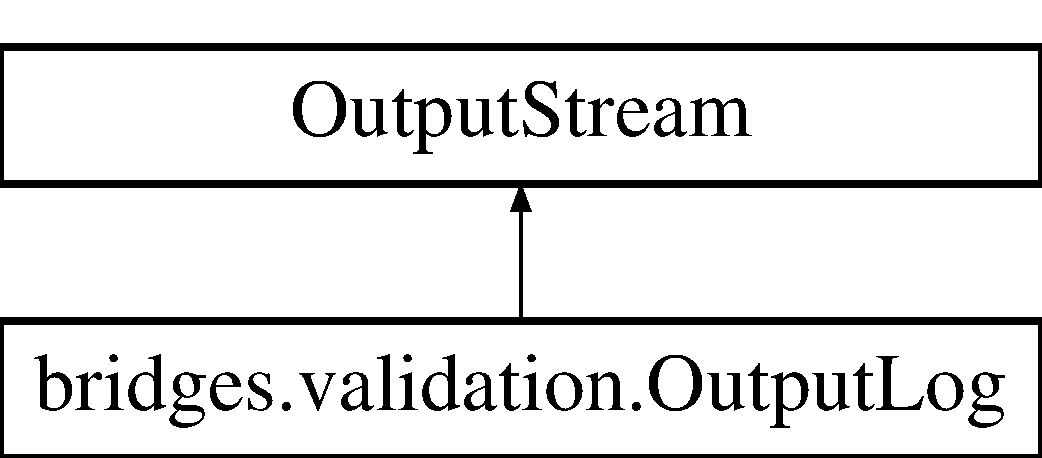
\includegraphics[height=2.000000cm]{classbridges_1_1validation_1_1_output_log}
\end{center}
\end{figure}
\subsection*{Public Member Functions}
\begin{DoxyCompactItemize}
\item 
\hyperlink{classbridges_1_1validation_1_1_output_log_a47a7efee1dce6f11f3de83d48994a56f}{Output\+Log} ()
\item 
boolean \hyperlink{classbridges_1_1validation_1_1_output_log_aae5e41b4b23adb56e3c97d2c17ad0768}{record\+Log} ()
\item 
boolean \hyperlink{classbridges_1_1validation_1_1_output_log_a4ec6037db31ff9dc0664d341183f296f}{return\+Stream} ()  throws I\+O\+Exception 
\item 
void \hyperlink{classbridges_1_1validation_1_1_output_log_a68ed2055f1a0626674675354feeb9d54}{write} (int b)  throws I\+O\+Exception 
\item 
void \hyperlink{classbridges_1_1validation_1_1_output_log_a6489f70aa4e2903456ed05315dd59f31}{write} (byte\mbox{[}$\,$\mbox{]} b)  throws I\+O\+Exception 
\item 
void \hyperlink{classbridges_1_1validation_1_1_output_log_ad0ada8f6ff72218f18b64672690fc94f}{write} (byte\mbox{[}$\,$\mbox{]} b, int a, int lenght)  throws I\+O\+Exception 
\item 
void \hyperlink{classbridges_1_1validation_1_1_output_log_a6ab7881cd35aa11cc830dab4732fe66d}{close} ()  throws I\+O\+Exception 
\item 
void \hyperlink{classbridges_1_1validation_1_1_output_log_ab810fd1e3d7e939bcdf1ec38978c02cd}{flush} ()  throws I\+O\+Exception 
\item 
void \hyperlink{classbridges_1_1validation_1_1_output_log_aea898d0de8715c1451d4731f3d9ae91d}{log\+Message} ()
\end{DoxyCompactItemize}
\subsection*{Static Public Member Functions}
\begin{DoxyCompactItemize}
\item 
static void \hyperlink{classbridges_1_1validation_1_1_output_log_a049b3ecad1138f73207d69b1193fe2e6}{split\+Stream} ()
\end{DoxyCompactItemize}
\subsection*{Static Protected Attributes}
\begin{DoxyCompactItemize}
\item 
static Print\+Stream \hyperlink{classbridges_1_1validation_1_1_output_log_a0f6ae61da2727193baf2d79a78f68614}{captured\+Stream}
\item 
static Print\+Stream \hyperlink{classbridges_1_1validation_1_1_output_log_acf8b19de1738e70f12eba5854b9e01b4}{new\+Output\+Stream}
\item 
static Print\+Stream \hyperlink{classbridges_1_1validation_1_1_output_log_a007a8494bdda0f4164663df8afe2c392}{log\+Stream}
\item 
static Print\+Stream \hyperlink{classbridges_1_1validation_1_1_output_log_a3b5198266da9d86da13fab21c096f18c}{log\+Stream2}
\item 
static File\+Output\+Stream \hyperlink{classbridges_1_1validation_1_1_output_log_a0e10e95bbb841f1f17b3b363461db3f3}{log\+File}
\item 
static Byte\+Array\+Output\+Stream \hyperlink{classbridges_1_1validation_1_1_output_log_a142611812dd1ea095c4a1274bd40a93a}{temp1}
\item 
static Byte\+Array\+Output\+Stream \hyperlink{classbridges_1_1validation_1_1_output_log_ab1f0ab7e9ada60f29c4c4f59694c1163}{temp2}
\item 
static String \hyperlink{classbridges_1_1validation_1_1_output_log_a74d7353fe97c80b3880825d18d7ccaa5}{a\+Path\+To\+Log}
\end{DoxyCompactItemize}


\subsection{Constructor \& Destructor Documentation}
\mbox{\Hypertarget{classbridges_1_1validation_1_1_output_log_a47a7efee1dce6f11f3de83d48994a56f}\label{classbridges_1_1validation_1_1_output_log_a47a7efee1dce6f11f3de83d48994a56f}} 
\index{bridges\+::validation\+::\+Output\+Log@{bridges\+::validation\+::\+Output\+Log}!Output\+Log@{Output\+Log}}
\index{Output\+Log@{Output\+Log}!bridges\+::validation\+::\+Output\+Log@{bridges\+::validation\+::\+Output\+Log}}
\subsubsection{\texorpdfstring{Output\+Log()}{OutputLog()}}
{\footnotesize\ttfamily bridges.\+validation.\+Output\+Log.\+Output\+Log (\begin{DoxyParamCaption}{ }\end{DoxyParamCaption})}

Constructor 

\subsection{Member Function Documentation}
\mbox{\Hypertarget{classbridges_1_1validation_1_1_output_log_a6ab7881cd35aa11cc830dab4732fe66d}\label{classbridges_1_1validation_1_1_output_log_a6ab7881cd35aa11cc830dab4732fe66d}} 
\index{bridges\+::validation\+::\+Output\+Log@{bridges\+::validation\+::\+Output\+Log}!close@{close}}
\index{close@{close}!bridges\+::validation\+::\+Output\+Log@{bridges\+::validation\+::\+Output\+Log}}
\subsubsection{\texorpdfstring{close()}{close()}}
{\footnotesize\ttfamily void bridges.\+validation.\+Output\+Log.\+close (\begin{DoxyParamCaption}{ }\end{DoxyParamCaption}) throws I\+O\+Exception}

\mbox{\Hypertarget{classbridges_1_1validation_1_1_output_log_ab810fd1e3d7e939bcdf1ec38978c02cd}\label{classbridges_1_1validation_1_1_output_log_ab810fd1e3d7e939bcdf1ec38978c02cd}} 
\index{bridges\+::validation\+::\+Output\+Log@{bridges\+::validation\+::\+Output\+Log}!flush@{flush}}
\index{flush@{flush}!bridges\+::validation\+::\+Output\+Log@{bridges\+::validation\+::\+Output\+Log}}
\subsubsection{\texorpdfstring{flush()}{flush()}}
{\footnotesize\ttfamily void bridges.\+validation.\+Output\+Log.\+flush (\begin{DoxyParamCaption}{ }\end{DoxyParamCaption}) throws I\+O\+Exception}

\mbox{\Hypertarget{classbridges_1_1validation_1_1_output_log_aea898d0de8715c1451d4731f3d9ae91d}\label{classbridges_1_1validation_1_1_output_log_aea898d0de8715c1451d4731f3d9ae91d}} 
\index{bridges\+::validation\+::\+Output\+Log@{bridges\+::validation\+::\+Output\+Log}!log\+Message@{log\+Message}}
\index{log\+Message@{log\+Message}!bridges\+::validation\+::\+Output\+Log@{bridges\+::validation\+::\+Output\+Log}}
\subsubsection{\texorpdfstring{log\+Message()}{logMessage()}}
{\footnotesize\ttfamily void bridges.\+validation.\+Output\+Log.\+log\+Message (\begin{DoxyParamCaption}{ }\end{DoxyParamCaption})}

This prints the Logger message to standard output \mbox{\Hypertarget{classbridges_1_1validation_1_1_output_log_aae5e41b4b23adb56e3c97d2c17ad0768}\label{classbridges_1_1validation_1_1_output_log_aae5e41b4b23adb56e3c97d2c17ad0768}} 
\index{bridges\+::validation\+::\+Output\+Log@{bridges\+::validation\+::\+Output\+Log}!record\+Log@{record\+Log}}
\index{record\+Log@{record\+Log}!bridges\+::validation\+::\+Output\+Log@{bridges\+::validation\+::\+Output\+Log}}
\subsubsection{\texorpdfstring{record\+Log()}{recordLog()}}
{\footnotesize\ttfamily boolean bridges.\+validation.\+Output\+Log.\+record\+Log (\begin{DoxyParamCaption}{ }\end{DoxyParamCaption})}

This method records the time stamp to the current log entry \begin{DoxyReturn}{Returns}
boolean 
\end{DoxyReturn}
\mbox{\Hypertarget{classbridges_1_1validation_1_1_output_log_a4ec6037db31ff9dc0664d341183f296f}\label{classbridges_1_1validation_1_1_output_log_a4ec6037db31ff9dc0664d341183f296f}} 
\index{bridges\+::validation\+::\+Output\+Log@{bridges\+::validation\+::\+Output\+Log}!return\+Stream@{return\+Stream}}
\index{return\+Stream@{return\+Stream}!bridges\+::validation\+::\+Output\+Log@{bridges\+::validation\+::\+Output\+Log}}
\subsubsection{\texorpdfstring{return\+Stream()}{returnStream()}}
{\footnotesize\ttfamily boolean bridges.\+validation.\+Output\+Log.\+return\+Stream (\begin{DoxyParamCaption}{ }\end{DoxyParamCaption}) throws I\+O\+Exception}

This method returns the stream to standard output \begin{DoxyReturn}{Returns}
boolean 
\end{DoxyReturn}
\mbox{\Hypertarget{classbridges_1_1validation_1_1_output_log_a049b3ecad1138f73207d69b1193fe2e6}\label{classbridges_1_1validation_1_1_output_log_a049b3ecad1138f73207d69b1193fe2e6}} 
\index{bridges\+::validation\+::\+Output\+Log@{bridges\+::validation\+::\+Output\+Log}!split\+Stream@{split\+Stream}}
\index{split\+Stream@{split\+Stream}!bridges\+::validation\+::\+Output\+Log@{bridges\+::validation\+::\+Output\+Log}}
\subsubsection{\texorpdfstring{split\+Stream()}{splitStream()}}
{\footnotesize\ttfamily static void bridges.\+validation.\+Output\+Log.\+split\+Stream (\begin{DoxyParamCaption}{ }\end{DoxyParamCaption})\hspace{0.3cm}{\ttfamily [static]}}

This method redirects the IO stream \mbox{\Hypertarget{classbridges_1_1validation_1_1_output_log_a68ed2055f1a0626674675354feeb9d54}\label{classbridges_1_1validation_1_1_output_log_a68ed2055f1a0626674675354feeb9d54}} 
\index{bridges\+::validation\+::\+Output\+Log@{bridges\+::validation\+::\+Output\+Log}!write@{write}}
\index{write@{write}!bridges\+::validation\+::\+Output\+Log@{bridges\+::validation\+::\+Output\+Log}}
\subsubsection{\texorpdfstring{write()}{write()}\hspace{0.1cm}{\footnotesize\ttfamily [1/3]}}
{\footnotesize\ttfamily void bridges.\+validation.\+Output\+Log.\+write (\begin{DoxyParamCaption}\item[{int}]{b }\end{DoxyParamCaption}) throws I\+O\+Exception}

\mbox{\Hypertarget{classbridges_1_1validation_1_1_output_log_a6489f70aa4e2903456ed05315dd59f31}\label{classbridges_1_1validation_1_1_output_log_a6489f70aa4e2903456ed05315dd59f31}} 
\index{bridges\+::validation\+::\+Output\+Log@{bridges\+::validation\+::\+Output\+Log}!write@{write}}
\index{write@{write}!bridges\+::validation\+::\+Output\+Log@{bridges\+::validation\+::\+Output\+Log}}
\subsubsection{\texorpdfstring{write()}{write()}\hspace{0.1cm}{\footnotesize\ttfamily [2/3]}}
{\footnotesize\ttfamily void bridges.\+validation.\+Output\+Log.\+write (\begin{DoxyParamCaption}\item[{byte \mbox{[}$\,$\mbox{]}}]{b }\end{DoxyParamCaption}) throws I\+O\+Exception}

\mbox{\Hypertarget{classbridges_1_1validation_1_1_output_log_ad0ada8f6ff72218f18b64672690fc94f}\label{classbridges_1_1validation_1_1_output_log_ad0ada8f6ff72218f18b64672690fc94f}} 
\index{bridges\+::validation\+::\+Output\+Log@{bridges\+::validation\+::\+Output\+Log}!write@{write}}
\index{write@{write}!bridges\+::validation\+::\+Output\+Log@{bridges\+::validation\+::\+Output\+Log}}
\subsubsection{\texorpdfstring{write()}{write()}\hspace{0.1cm}{\footnotesize\ttfamily [3/3]}}
{\footnotesize\ttfamily void bridges.\+validation.\+Output\+Log.\+write (\begin{DoxyParamCaption}\item[{byte \mbox{[}$\,$\mbox{]}}]{b,  }\item[{int}]{a,  }\item[{int}]{lenght }\end{DoxyParamCaption}) throws I\+O\+Exception}



\subsection{Member Data Documentation}
\mbox{\Hypertarget{classbridges_1_1validation_1_1_output_log_a74d7353fe97c80b3880825d18d7ccaa5}\label{classbridges_1_1validation_1_1_output_log_a74d7353fe97c80b3880825d18d7ccaa5}} 
\index{bridges\+::validation\+::\+Output\+Log@{bridges\+::validation\+::\+Output\+Log}!a\+Path\+To\+Log@{a\+Path\+To\+Log}}
\index{a\+Path\+To\+Log@{a\+Path\+To\+Log}!bridges\+::validation\+::\+Output\+Log@{bridges\+::validation\+::\+Output\+Log}}
\subsubsection{\texorpdfstring{a\+Path\+To\+Log}{aPathToLog}}
{\footnotesize\ttfamily String bridges.\+validation.\+Output\+Log.\+a\+Path\+To\+Log\hspace{0.3cm}{\ttfamily [static]}, {\ttfamily [protected]}}

\mbox{\Hypertarget{classbridges_1_1validation_1_1_output_log_a0f6ae61da2727193baf2d79a78f68614}\label{classbridges_1_1validation_1_1_output_log_a0f6ae61da2727193baf2d79a78f68614}} 
\index{bridges\+::validation\+::\+Output\+Log@{bridges\+::validation\+::\+Output\+Log}!captured\+Stream@{captured\+Stream}}
\index{captured\+Stream@{captured\+Stream}!bridges\+::validation\+::\+Output\+Log@{bridges\+::validation\+::\+Output\+Log}}
\subsubsection{\texorpdfstring{captured\+Stream}{capturedStream}}
{\footnotesize\ttfamily Print\+Stream bridges.\+validation.\+Output\+Log.\+captured\+Stream\hspace{0.3cm}{\ttfamily [static]}, {\ttfamily [protected]}}

\mbox{\Hypertarget{classbridges_1_1validation_1_1_output_log_a0e10e95bbb841f1f17b3b363461db3f3}\label{classbridges_1_1validation_1_1_output_log_a0e10e95bbb841f1f17b3b363461db3f3}} 
\index{bridges\+::validation\+::\+Output\+Log@{bridges\+::validation\+::\+Output\+Log}!log\+File@{log\+File}}
\index{log\+File@{log\+File}!bridges\+::validation\+::\+Output\+Log@{bridges\+::validation\+::\+Output\+Log}}
\subsubsection{\texorpdfstring{log\+File}{logFile}}
{\footnotesize\ttfamily File\+Output\+Stream bridges.\+validation.\+Output\+Log.\+log\+File\hspace{0.3cm}{\ttfamily [static]}, {\ttfamily [protected]}}

\mbox{\Hypertarget{classbridges_1_1validation_1_1_output_log_a007a8494bdda0f4164663df8afe2c392}\label{classbridges_1_1validation_1_1_output_log_a007a8494bdda0f4164663df8afe2c392}} 
\index{bridges\+::validation\+::\+Output\+Log@{bridges\+::validation\+::\+Output\+Log}!log\+Stream@{log\+Stream}}
\index{log\+Stream@{log\+Stream}!bridges\+::validation\+::\+Output\+Log@{bridges\+::validation\+::\+Output\+Log}}
\subsubsection{\texorpdfstring{log\+Stream}{logStream}}
{\footnotesize\ttfamily Print\+Stream bridges.\+validation.\+Output\+Log.\+log\+Stream\hspace{0.3cm}{\ttfamily [static]}, {\ttfamily [protected]}}

\mbox{\Hypertarget{classbridges_1_1validation_1_1_output_log_a3b5198266da9d86da13fab21c096f18c}\label{classbridges_1_1validation_1_1_output_log_a3b5198266da9d86da13fab21c096f18c}} 
\index{bridges\+::validation\+::\+Output\+Log@{bridges\+::validation\+::\+Output\+Log}!log\+Stream2@{log\+Stream2}}
\index{log\+Stream2@{log\+Stream2}!bridges\+::validation\+::\+Output\+Log@{bridges\+::validation\+::\+Output\+Log}}
\subsubsection{\texorpdfstring{log\+Stream2}{logStream2}}
{\footnotesize\ttfamily Print\+Stream bridges.\+validation.\+Output\+Log.\+log\+Stream2\hspace{0.3cm}{\ttfamily [static]}, {\ttfamily [protected]}}

\mbox{\Hypertarget{classbridges_1_1validation_1_1_output_log_acf8b19de1738e70f12eba5854b9e01b4}\label{classbridges_1_1validation_1_1_output_log_acf8b19de1738e70f12eba5854b9e01b4}} 
\index{bridges\+::validation\+::\+Output\+Log@{bridges\+::validation\+::\+Output\+Log}!new\+Output\+Stream@{new\+Output\+Stream}}
\index{new\+Output\+Stream@{new\+Output\+Stream}!bridges\+::validation\+::\+Output\+Log@{bridges\+::validation\+::\+Output\+Log}}
\subsubsection{\texorpdfstring{new\+Output\+Stream}{newOutputStream}}
{\footnotesize\ttfamily Print\+Stream bridges.\+validation.\+Output\+Log.\+new\+Output\+Stream\hspace{0.3cm}{\ttfamily [static]}, {\ttfamily [protected]}}

\mbox{\Hypertarget{classbridges_1_1validation_1_1_output_log_a142611812dd1ea095c4a1274bd40a93a}\label{classbridges_1_1validation_1_1_output_log_a142611812dd1ea095c4a1274bd40a93a}} 
\index{bridges\+::validation\+::\+Output\+Log@{bridges\+::validation\+::\+Output\+Log}!temp1@{temp1}}
\index{temp1@{temp1}!bridges\+::validation\+::\+Output\+Log@{bridges\+::validation\+::\+Output\+Log}}
\subsubsection{\texorpdfstring{temp1}{temp1}}
{\footnotesize\ttfamily Byte\+Array\+Output\+Stream bridges.\+validation.\+Output\+Log.\+temp1\hspace{0.3cm}{\ttfamily [static]}, {\ttfamily [protected]}}

\mbox{\Hypertarget{classbridges_1_1validation_1_1_output_log_ab1f0ab7e9ada60f29c4c4f59694c1163}\label{classbridges_1_1validation_1_1_output_log_ab1f0ab7e9ada60f29c4c4f59694c1163}} 
\index{bridges\+::validation\+::\+Output\+Log@{bridges\+::validation\+::\+Output\+Log}!temp2@{temp2}}
\index{temp2@{temp2}!bridges\+::validation\+::\+Output\+Log@{bridges\+::validation\+::\+Output\+Log}}
\subsubsection{\texorpdfstring{temp2}{temp2}}
{\footnotesize\ttfamily Byte\+Array\+Output\+Stream bridges.\+validation.\+Output\+Log.\+temp2\hspace{0.3cm}{\ttfamily [static]}, {\ttfamily [protected]}}



The documentation for this class was generated from the following file\+:\begin{DoxyCompactItemize}
\item 
/home/erik/work/bridges/bridges-\/java/src/main/java/bridges/validation/\hyperlink{_output_log_8java}{Output\+Log.\+java}\end{DoxyCompactItemize}

\hypertarget{classbridges_1_1data__src__dependent_1_1_usgs_foo_1_1_properties}{}\section{bridges.\+data\+\_\+src\+\_\+dependent.\+Usgs\+Foo.\+Properties Class Reference}
\label{classbridges_1_1data__src__dependent_1_1_usgs_foo_1_1_properties}\index{bridges.\+data\+\_\+src\+\_\+dependent.\+Usgs\+Foo.\+Properties@{bridges.\+data\+\_\+src\+\_\+dependent.\+Usgs\+Foo.\+Properties}}
\subsection*{Public Member Functions}
\begin{DoxyCompactItemize}
\item 
String \hyperlink{classbridges_1_1data__src__dependent_1_1_usgs_foo_1_1_properties_a9dcb3ec22a3aaa828d79c7a41b1d9685}{get\+Mag} ()
\item 
void \hyperlink{classbridges_1_1data__src__dependent_1_1_usgs_foo_1_1_properties_aac22cfb93d78259f098f4f996313429c}{set\+Mag} (String \hyperlink{classbridges_1_1data__src__dependent_1_1_usgs_foo_1_1_properties_a114163b5773ae63dc7554d0fb365f540}{mag})
\item 
String \hyperlink{classbridges_1_1data__src__dependent_1_1_usgs_foo_1_1_properties_ae97633cdfd1a3c6420ea7c38ed4155a2}{get\+Place} ()
\item 
void \hyperlink{classbridges_1_1data__src__dependent_1_1_usgs_foo_1_1_properties_a62e8d04129240c4f04b880ab2fef1f04}{set\+Place} (String \hyperlink{classbridges_1_1data__src__dependent_1_1_usgs_foo_1_1_properties_a78104fd6df6eec29b1598669127df9ed}{place})
\item 
String \hyperlink{classbridges_1_1data__src__dependent_1_1_usgs_foo_1_1_properties_abf80c8378da2b28708f49e9cf5bdf2d8}{get\+Time} ()
\item 
void \hyperlink{classbridges_1_1data__src__dependent_1_1_usgs_foo_1_1_properties_a846ac9ec8c49cd261a7dec80844fef27}{set\+Time} (String \hyperlink{classbridges_1_1data__src__dependent_1_1_usgs_foo_1_1_properties_a6e42210e723e44d15bcea954ccd6b579}{time})
\item 
String \hyperlink{classbridges_1_1data__src__dependent_1_1_usgs_foo_1_1_properties_a730443f40e47ba5ca0ed1c7005153ed2}{get\+Title} ()
\item 
void \hyperlink{classbridges_1_1data__src__dependent_1_1_usgs_foo_1_1_properties_aa22752d66c3427eac4559a24a79a6cd8}{set\+Title} (String \hyperlink{classbridges_1_1data__src__dependent_1_1_usgs_foo_1_1_properties_a8ffe112286f04d57850831222e1c50d6}{title})
\item 
String \hyperlink{classbridges_1_1data__src__dependent_1_1_usgs_foo_1_1_properties_a7a2ccdc56c0e935cf4f262e51f40f4ea}{get\+Url} ()
\item 
void \hyperlink{classbridges_1_1data__src__dependent_1_1_usgs_foo_1_1_properties_a9dae43b92463eb6abbcc888854bf9afa}{set\+Url} (String \hyperlink{classbridges_1_1data__src__dependent_1_1_usgs_foo_1_1_properties_a42e5d1f2c28c6708921861ed95aa5e5f}{url})
\item 
String \hyperlink{classbridges_1_1data__src__dependent_1_1_usgs_foo_1_1_properties_add3d2aeb53fec22ccec06b288058e416}{to\+String} ()
\end{DoxyCompactItemize}
\subsection*{Public Attributes}
\begin{DoxyCompactItemize}
\item 
String \hyperlink{classbridges_1_1data__src__dependent_1_1_usgs_foo_1_1_properties_a114163b5773ae63dc7554d0fb365f540}{mag}
\item 
String \hyperlink{classbridges_1_1data__src__dependent_1_1_usgs_foo_1_1_properties_a78104fd6df6eec29b1598669127df9ed}{place}
\item 
String \hyperlink{classbridges_1_1data__src__dependent_1_1_usgs_foo_1_1_properties_a6e42210e723e44d15bcea954ccd6b579}{time}
\item 
String \hyperlink{classbridges_1_1data__src__dependent_1_1_usgs_foo_1_1_properties_a8ffe112286f04d57850831222e1c50d6}{title}
\item 
String \hyperlink{classbridges_1_1data__src__dependent_1_1_usgs_foo_1_1_properties_a42e5d1f2c28c6708921861ed95aa5e5f}{url}
\end{DoxyCompactItemize}


\subsection{Member Function Documentation}
\hypertarget{classbridges_1_1data__src__dependent_1_1_usgs_foo_1_1_properties_a9dcb3ec22a3aaa828d79c7a41b1d9685}{}\index{bridges\+::data\+\_\+src\+\_\+dependent\+::\+Usgs\+Foo\+::\+Properties@{bridges\+::data\+\_\+src\+\_\+dependent\+::\+Usgs\+Foo\+::\+Properties}!get\+Mag@{get\+Mag}}
\index{get\+Mag@{get\+Mag}!bridges\+::data\+\_\+src\+\_\+dependent\+::\+Usgs\+Foo\+::\+Properties@{bridges\+::data\+\_\+src\+\_\+dependent\+::\+Usgs\+Foo\+::\+Properties}}
\subsubsection[{get\+Mag()}]{\setlength{\rightskip}{0pt plus 5cm}String bridges.\+data\+\_\+src\+\_\+dependent.\+Usgs\+Foo.\+Properties.\+get\+Mag (
\begin{DoxyParamCaption}
{}
\end{DoxyParamCaption}
)}\label{classbridges_1_1data__src__dependent_1_1_usgs_foo_1_1_properties_a9dcb3ec22a3aaa828d79c7a41b1d9685}
\hypertarget{classbridges_1_1data__src__dependent_1_1_usgs_foo_1_1_properties_ae97633cdfd1a3c6420ea7c38ed4155a2}{}\index{bridges\+::data\+\_\+src\+\_\+dependent\+::\+Usgs\+Foo\+::\+Properties@{bridges\+::data\+\_\+src\+\_\+dependent\+::\+Usgs\+Foo\+::\+Properties}!get\+Place@{get\+Place}}
\index{get\+Place@{get\+Place}!bridges\+::data\+\_\+src\+\_\+dependent\+::\+Usgs\+Foo\+::\+Properties@{bridges\+::data\+\_\+src\+\_\+dependent\+::\+Usgs\+Foo\+::\+Properties}}
\subsubsection[{get\+Place()}]{\setlength{\rightskip}{0pt plus 5cm}String bridges.\+data\+\_\+src\+\_\+dependent.\+Usgs\+Foo.\+Properties.\+get\+Place (
\begin{DoxyParamCaption}
{}
\end{DoxyParamCaption}
)}\label{classbridges_1_1data__src__dependent_1_1_usgs_foo_1_1_properties_ae97633cdfd1a3c6420ea7c38ed4155a2}
\hypertarget{classbridges_1_1data__src__dependent_1_1_usgs_foo_1_1_properties_abf80c8378da2b28708f49e9cf5bdf2d8}{}\index{bridges\+::data\+\_\+src\+\_\+dependent\+::\+Usgs\+Foo\+::\+Properties@{bridges\+::data\+\_\+src\+\_\+dependent\+::\+Usgs\+Foo\+::\+Properties}!get\+Time@{get\+Time}}
\index{get\+Time@{get\+Time}!bridges\+::data\+\_\+src\+\_\+dependent\+::\+Usgs\+Foo\+::\+Properties@{bridges\+::data\+\_\+src\+\_\+dependent\+::\+Usgs\+Foo\+::\+Properties}}
\subsubsection[{get\+Time()}]{\setlength{\rightskip}{0pt plus 5cm}String bridges.\+data\+\_\+src\+\_\+dependent.\+Usgs\+Foo.\+Properties.\+get\+Time (
\begin{DoxyParamCaption}
{}
\end{DoxyParamCaption}
)}\label{classbridges_1_1data__src__dependent_1_1_usgs_foo_1_1_properties_abf80c8378da2b28708f49e9cf5bdf2d8}
\hypertarget{classbridges_1_1data__src__dependent_1_1_usgs_foo_1_1_properties_a730443f40e47ba5ca0ed1c7005153ed2}{}\index{bridges\+::data\+\_\+src\+\_\+dependent\+::\+Usgs\+Foo\+::\+Properties@{bridges\+::data\+\_\+src\+\_\+dependent\+::\+Usgs\+Foo\+::\+Properties}!get\+Title@{get\+Title}}
\index{get\+Title@{get\+Title}!bridges\+::data\+\_\+src\+\_\+dependent\+::\+Usgs\+Foo\+::\+Properties@{bridges\+::data\+\_\+src\+\_\+dependent\+::\+Usgs\+Foo\+::\+Properties}}
\subsubsection[{get\+Title()}]{\setlength{\rightskip}{0pt plus 5cm}String bridges.\+data\+\_\+src\+\_\+dependent.\+Usgs\+Foo.\+Properties.\+get\+Title (
\begin{DoxyParamCaption}
{}
\end{DoxyParamCaption}
)}\label{classbridges_1_1data__src__dependent_1_1_usgs_foo_1_1_properties_a730443f40e47ba5ca0ed1c7005153ed2}
\hypertarget{classbridges_1_1data__src__dependent_1_1_usgs_foo_1_1_properties_a7a2ccdc56c0e935cf4f262e51f40f4ea}{}\index{bridges\+::data\+\_\+src\+\_\+dependent\+::\+Usgs\+Foo\+::\+Properties@{bridges\+::data\+\_\+src\+\_\+dependent\+::\+Usgs\+Foo\+::\+Properties}!get\+Url@{get\+Url}}
\index{get\+Url@{get\+Url}!bridges\+::data\+\_\+src\+\_\+dependent\+::\+Usgs\+Foo\+::\+Properties@{bridges\+::data\+\_\+src\+\_\+dependent\+::\+Usgs\+Foo\+::\+Properties}}
\subsubsection[{get\+Url()}]{\setlength{\rightskip}{0pt plus 5cm}String bridges.\+data\+\_\+src\+\_\+dependent.\+Usgs\+Foo.\+Properties.\+get\+Url (
\begin{DoxyParamCaption}
{}
\end{DoxyParamCaption}
)}\label{classbridges_1_1data__src__dependent_1_1_usgs_foo_1_1_properties_a7a2ccdc56c0e935cf4f262e51f40f4ea}
\hypertarget{classbridges_1_1data__src__dependent_1_1_usgs_foo_1_1_properties_aac22cfb93d78259f098f4f996313429c}{}\index{bridges\+::data\+\_\+src\+\_\+dependent\+::\+Usgs\+Foo\+::\+Properties@{bridges\+::data\+\_\+src\+\_\+dependent\+::\+Usgs\+Foo\+::\+Properties}!set\+Mag@{set\+Mag}}
\index{set\+Mag@{set\+Mag}!bridges\+::data\+\_\+src\+\_\+dependent\+::\+Usgs\+Foo\+::\+Properties@{bridges\+::data\+\_\+src\+\_\+dependent\+::\+Usgs\+Foo\+::\+Properties}}
\subsubsection[{set\+Mag(\+String mag)}]{\setlength{\rightskip}{0pt plus 5cm}void bridges.\+data\+\_\+src\+\_\+dependent.\+Usgs\+Foo.\+Properties.\+set\+Mag (
\begin{DoxyParamCaption}
\item[{String}]{mag}
\end{DoxyParamCaption}
)}\label{classbridges_1_1data__src__dependent_1_1_usgs_foo_1_1_properties_aac22cfb93d78259f098f4f996313429c}
\hypertarget{classbridges_1_1data__src__dependent_1_1_usgs_foo_1_1_properties_a62e8d04129240c4f04b880ab2fef1f04}{}\index{bridges\+::data\+\_\+src\+\_\+dependent\+::\+Usgs\+Foo\+::\+Properties@{bridges\+::data\+\_\+src\+\_\+dependent\+::\+Usgs\+Foo\+::\+Properties}!set\+Place@{set\+Place}}
\index{set\+Place@{set\+Place}!bridges\+::data\+\_\+src\+\_\+dependent\+::\+Usgs\+Foo\+::\+Properties@{bridges\+::data\+\_\+src\+\_\+dependent\+::\+Usgs\+Foo\+::\+Properties}}
\subsubsection[{set\+Place(\+String place)}]{\setlength{\rightskip}{0pt plus 5cm}void bridges.\+data\+\_\+src\+\_\+dependent.\+Usgs\+Foo.\+Properties.\+set\+Place (
\begin{DoxyParamCaption}
\item[{String}]{place}
\end{DoxyParamCaption}
)}\label{classbridges_1_1data__src__dependent_1_1_usgs_foo_1_1_properties_a62e8d04129240c4f04b880ab2fef1f04}
\hypertarget{classbridges_1_1data__src__dependent_1_1_usgs_foo_1_1_properties_a846ac9ec8c49cd261a7dec80844fef27}{}\index{bridges\+::data\+\_\+src\+\_\+dependent\+::\+Usgs\+Foo\+::\+Properties@{bridges\+::data\+\_\+src\+\_\+dependent\+::\+Usgs\+Foo\+::\+Properties}!set\+Time@{set\+Time}}
\index{set\+Time@{set\+Time}!bridges\+::data\+\_\+src\+\_\+dependent\+::\+Usgs\+Foo\+::\+Properties@{bridges\+::data\+\_\+src\+\_\+dependent\+::\+Usgs\+Foo\+::\+Properties}}
\subsubsection[{set\+Time(\+String time)}]{\setlength{\rightskip}{0pt plus 5cm}void bridges.\+data\+\_\+src\+\_\+dependent.\+Usgs\+Foo.\+Properties.\+set\+Time (
\begin{DoxyParamCaption}
\item[{String}]{time}
\end{DoxyParamCaption}
)}\label{classbridges_1_1data__src__dependent_1_1_usgs_foo_1_1_properties_a846ac9ec8c49cd261a7dec80844fef27}
\hypertarget{classbridges_1_1data__src__dependent_1_1_usgs_foo_1_1_properties_aa22752d66c3427eac4559a24a79a6cd8}{}\index{bridges\+::data\+\_\+src\+\_\+dependent\+::\+Usgs\+Foo\+::\+Properties@{bridges\+::data\+\_\+src\+\_\+dependent\+::\+Usgs\+Foo\+::\+Properties}!set\+Title@{set\+Title}}
\index{set\+Title@{set\+Title}!bridges\+::data\+\_\+src\+\_\+dependent\+::\+Usgs\+Foo\+::\+Properties@{bridges\+::data\+\_\+src\+\_\+dependent\+::\+Usgs\+Foo\+::\+Properties}}
\subsubsection[{set\+Title(\+String title)}]{\setlength{\rightskip}{0pt plus 5cm}void bridges.\+data\+\_\+src\+\_\+dependent.\+Usgs\+Foo.\+Properties.\+set\+Title (
\begin{DoxyParamCaption}
\item[{String}]{title}
\end{DoxyParamCaption}
)}\label{classbridges_1_1data__src__dependent_1_1_usgs_foo_1_1_properties_aa22752d66c3427eac4559a24a79a6cd8}
\hypertarget{classbridges_1_1data__src__dependent_1_1_usgs_foo_1_1_properties_a9dae43b92463eb6abbcc888854bf9afa}{}\index{bridges\+::data\+\_\+src\+\_\+dependent\+::\+Usgs\+Foo\+::\+Properties@{bridges\+::data\+\_\+src\+\_\+dependent\+::\+Usgs\+Foo\+::\+Properties}!set\+Url@{set\+Url}}
\index{set\+Url@{set\+Url}!bridges\+::data\+\_\+src\+\_\+dependent\+::\+Usgs\+Foo\+::\+Properties@{bridges\+::data\+\_\+src\+\_\+dependent\+::\+Usgs\+Foo\+::\+Properties}}
\subsubsection[{set\+Url(\+String url)}]{\setlength{\rightskip}{0pt plus 5cm}void bridges.\+data\+\_\+src\+\_\+dependent.\+Usgs\+Foo.\+Properties.\+set\+Url (
\begin{DoxyParamCaption}
\item[{String}]{url}
\end{DoxyParamCaption}
)}\label{classbridges_1_1data__src__dependent_1_1_usgs_foo_1_1_properties_a9dae43b92463eb6abbcc888854bf9afa}
\hypertarget{classbridges_1_1data__src__dependent_1_1_usgs_foo_1_1_properties_add3d2aeb53fec22ccec06b288058e416}{}\index{bridges\+::data\+\_\+src\+\_\+dependent\+::\+Usgs\+Foo\+::\+Properties@{bridges\+::data\+\_\+src\+\_\+dependent\+::\+Usgs\+Foo\+::\+Properties}!to\+String@{to\+String}}
\index{to\+String@{to\+String}!bridges\+::data\+\_\+src\+\_\+dependent\+::\+Usgs\+Foo\+::\+Properties@{bridges\+::data\+\_\+src\+\_\+dependent\+::\+Usgs\+Foo\+::\+Properties}}
\subsubsection[{to\+String()}]{\setlength{\rightskip}{0pt plus 5cm}String bridges.\+data\+\_\+src\+\_\+dependent.\+Usgs\+Foo.\+Properties.\+to\+String (
\begin{DoxyParamCaption}
{}
\end{DoxyParamCaption}
)}\label{classbridges_1_1data__src__dependent_1_1_usgs_foo_1_1_properties_add3d2aeb53fec22ccec06b288058e416}


\subsection{Member Data Documentation}
\hypertarget{classbridges_1_1data__src__dependent_1_1_usgs_foo_1_1_properties_a114163b5773ae63dc7554d0fb365f540}{}\index{bridges\+::data\+\_\+src\+\_\+dependent\+::\+Usgs\+Foo\+::\+Properties@{bridges\+::data\+\_\+src\+\_\+dependent\+::\+Usgs\+Foo\+::\+Properties}!mag@{mag}}
\index{mag@{mag}!bridges\+::data\+\_\+src\+\_\+dependent\+::\+Usgs\+Foo\+::\+Properties@{bridges\+::data\+\_\+src\+\_\+dependent\+::\+Usgs\+Foo\+::\+Properties}}
\subsubsection[{mag}]{\setlength{\rightskip}{0pt plus 5cm}String bridges.\+data\+\_\+src\+\_\+dependent.\+Usgs\+Foo.\+Properties.\+mag}\label{classbridges_1_1data__src__dependent_1_1_usgs_foo_1_1_properties_a114163b5773ae63dc7554d0fb365f540}
\hypertarget{classbridges_1_1data__src__dependent_1_1_usgs_foo_1_1_properties_a78104fd6df6eec29b1598669127df9ed}{}\index{bridges\+::data\+\_\+src\+\_\+dependent\+::\+Usgs\+Foo\+::\+Properties@{bridges\+::data\+\_\+src\+\_\+dependent\+::\+Usgs\+Foo\+::\+Properties}!place@{place}}
\index{place@{place}!bridges\+::data\+\_\+src\+\_\+dependent\+::\+Usgs\+Foo\+::\+Properties@{bridges\+::data\+\_\+src\+\_\+dependent\+::\+Usgs\+Foo\+::\+Properties}}
\subsubsection[{place}]{\setlength{\rightskip}{0pt plus 5cm}String bridges.\+data\+\_\+src\+\_\+dependent.\+Usgs\+Foo.\+Properties.\+place}\label{classbridges_1_1data__src__dependent_1_1_usgs_foo_1_1_properties_a78104fd6df6eec29b1598669127df9ed}
\hypertarget{classbridges_1_1data__src__dependent_1_1_usgs_foo_1_1_properties_a6e42210e723e44d15bcea954ccd6b579}{}\index{bridges\+::data\+\_\+src\+\_\+dependent\+::\+Usgs\+Foo\+::\+Properties@{bridges\+::data\+\_\+src\+\_\+dependent\+::\+Usgs\+Foo\+::\+Properties}!time@{time}}
\index{time@{time}!bridges\+::data\+\_\+src\+\_\+dependent\+::\+Usgs\+Foo\+::\+Properties@{bridges\+::data\+\_\+src\+\_\+dependent\+::\+Usgs\+Foo\+::\+Properties}}
\subsubsection[{time}]{\setlength{\rightskip}{0pt plus 5cm}String bridges.\+data\+\_\+src\+\_\+dependent.\+Usgs\+Foo.\+Properties.\+time}\label{classbridges_1_1data__src__dependent_1_1_usgs_foo_1_1_properties_a6e42210e723e44d15bcea954ccd6b579}
\hypertarget{classbridges_1_1data__src__dependent_1_1_usgs_foo_1_1_properties_a8ffe112286f04d57850831222e1c50d6}{}\index{bridges\+::data\+\_\+src\+\_\+dependent\+::\+Usgs\+Foo\+::\+Properties@{bridges\+::data\+\_\+src\+\_\+dependent\+::\+Usgs\+Foo\+::\+Properties}!title@{title}}
\index{title@{title}!bridges\+::data\+\_\+src\+\_\+dependent\+::\+Usgs\+Foo\+::\+Properties@{bridges\+::data\+\_\+src\+\_\+dependent\+::\+Usgs\+Foo\+::\+Properties}}
\subsubsection[{title}]{\setlength{\rightskip}{0pt plus 5cm}String bridges.\+data\+\_\+src\+\_\+dependent.\+Usgs\+Foo.\+Properties.\+title}\label{classbridges_1_1data__src__dependent_1_1_usgs_foo_1_1_properties_a8ffe112286f04d57850831222e1c50d6}
\hypertarget{classbridges_1_1data__src__dependent_1_1_usgs_foo_1_1_properties_a42e5d1f2c28c6708921861ed95aa5e5f}{}\index{bridges\+::data\+\_\+src\+\_\+dependent\+::\+Usgs\+Foo\+::\+Properties@{bridges\+::data\+\_\+src\+\_\+dependent\+::\+Usgs\+Foo\+::\+Properties}!url@{url}}
\index{url@{url}!bridges\+::data\+\_\+src\+\_\+dependent\+::\+Usgs\+Foo\+::\+Properties@{bridges\+::data\+\_\+src\+\_\+dependent\+::\+Usgs\+Foo\+::\+Properties}}
\subsubsection[{url}]{\setlength{\rightskip}{0pt plus 5cm}String bridges.\+data\+\_\+src\+\_\+dependent.\+Usgs\+Foo.\+Properties.\+url}\label{classbridges_1_1data__src__dependent_1_1_usgs_foo_1_1_properties_a42e5d1f2c28c6708921861ed95aa5e5f}


The documentation for this class was generated from the following file\+:\begin{DoxyCompactItemize}
\item 
link/data\+\_\+src\+\_\+dependent/\hyperlink{_usgs_foo_8java}{Usgs\+Foo.\+java}\end{DoxyCompactItemize}

\hypertarget{classbridges_1_1validation_1_1_rate_limit_exception}{}\doxysection{bridges.\+validation.\+Rate\+Limit\+Exception Class Reference}
\label{classbridges_1_1validation_1_1_rate_limit_exception}\index{bridges.validation.RateLimitException@{bridges.validation.RateLimitException}}
Inheritance diagram for bridges.\+validation.\+Rate\+Limit\+Exception\+:\begin{figure}[H]
\begin{center}
\leavevmode
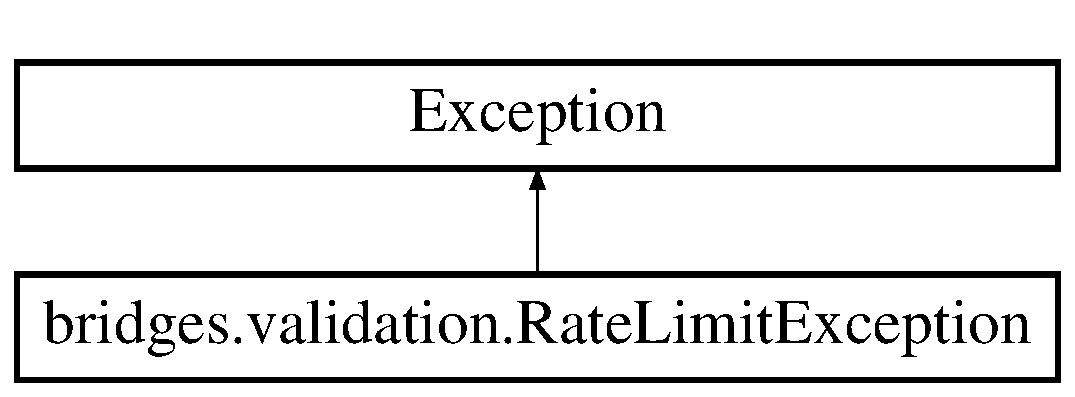
\includegraphics[height=2.000000cm]{classbridges_1_1validation_1_1_rate_limit_exception}
\end{center}
\end{figure}
\doxysubsection*{Public Member Functions}
\begin{DoxyCompactItemize}
\item 
\mbox{\hyperlink{classbridges_1_1validation_1_1_rate_limit_exception_a8375495a80a80213fe9201921c43afbc}{Rate\+Limit\+Exception}} (String string)
\end{DoxyCompactItemize}


\doxysubsection{Detailed Description}
Throws exception to handle overloading the server to allow the student to stop querying the server and send in their visualizations. This exception is expected every time the program runs to limit the amount of requests going to Twitter etc.

\begin{DoxyAuthor}{Author}
Michael 
\end{DoxyAuthor}


\doxysubsection{Constructor \& Destructor Documentation}
\mbox{\Hypertarget{classbridges_1_1validation_1_1_rate_limit_exception_a8375495a80a80213fe9201921c43afbc}\label{classbridges_1_1validation_1_1_rate_limit_exception_a8375495a80a80213fe9201921c43afbc}} 
\index{bridges.validation.RateLimitException@{bridges.validation.RateLimitException}!RateLimitException@{RateLimitException}}
\index{RateLimitException@{RateLimitException}!bridges.validation.RateLimitException@{bridges.validation.RateLimitException}}
\doxysubsubsection{\texorpdfstring{RateLimitException()}{RateLimitException()}}
{\footnotesize\ttfamily bridges.\+validation.\+Rate\+Limit\+Exception.\+Rate\+Limit\+Exception (\begin{DoxyParamCaption}\item[{String}]{string }\end{DoxyParamCaption})}



The documentation for this class was generated from the following file\+:\begin{DoxyCompactItemize}
\item 
/\+Users/kalpathi/gr/bridges/client/java/src/main/java/bridges/validation/\mbox{\hyperlink{_rate_limit_exception_8java}{Rate\+Limit\+Exception.\+java}}\end{DoxyCompactItemize}

\hypertarget{classbridges_1_1data__src__dependent_1_1_rotten_tomatos}{}\section{bridges.\+data\+\_\+src\+\_\+dependent.\+Rotten\+Tomatos Class Reference}
\label{classbridges_1_1data__src__dependent_1_1_rotten_tomatos}\index{bridges.data\_src\_dependent.RottenTomatos@{bridges.data\_src\_dependent.RottenTomatos}}


Inherits bridges.\+data\+\_\+src\+\_\+dependent.\+Data\+Source.

\subsection*{Public Member Functions}
\begin{DoxyCompactItemize}
\item 
\mbox{\hyperlink{classbridges_1_1data__src__dependent_1_1_rotten_tomatos_af18285905c6f2b944c5aa2cf7fbaf454}{Rotten\+Tomatos}} (String src)
\item 
void \mbox{\hyperlink{classbridges_1_1data__src__dependent_1_1_rotten_tomatos_a7edb12a260f8f309ba45825eff44e8e7}{set\+Label}} (String label)
\item 
String \mbox{\hyperlink{classbridges_1_1data__src__dependent_1_1_rotten_tomatos_a64c1b0e15a8a0104d4da2a5e3f0f09f7}{get\+Label}} ()
\item 
String \mbox{\hyperlink{classbridges_1_1data__src__dependent_1_1_rotten_tomatos_ae417dd4acab340041d2d88b0fd828784}{to\+String}} ()
\end{DoxyCompactItemize}


\subsection{Constructor \& Destructor Documentation}
\mbox{\Hypertarget{classbridges_1_1data__src__dependent_1_1_rotten_tomatos_af18285905c6f2b944c5aa2cf7fbaf454}\label{classbridges_1_1data__src__dependent_1_1_rotten_tomatos_af18285905c6f2b944c5aa2cf7fbaf454}} 
\index{bridges.data\_src\_dependent.RottenTomatos@{bridges.data\_src\_dependent.RottenTomatos}!RottenTomatos@{RottenTomatos}}
\index{RottenTomatos@{RottenTomatos}!bridges.data\_src\_dependent.RottenTomatos@{bridges.data\_src\_dependent.RottenTomatos}}
\subsubsection{\texorpdfstring{RottenTomatos()}{RottenTomatos()}}
{\footnotesize\ttfamily bridges.\+data\+\_\+src\+\_\+dependent.\+Rotten\+Tomatos.\+Rotten\+Tomatos (\begin{DoxyParamCaption}\item[{String}]{src }\end{DoxyParamCaption})}

Constructor 

\subsection{Member Function Documentation}
\mbox{\Hypertarget{classbridges_1_1data__src__dependent_1_1_rotten_tomatos_a64c1b0e15a8a0104d4da2a5e3f0f09f7}\label{classbridges_1_1data__src__dependent_1_1_rotten_tomatos_a64c1b0e15a8a0104d4da2a5e3f0f09f7}} 
\index{bridges.data\_src\_dependent.RottenTomatos@{bridges.data\_src\_dependent.RottenTomatos}!getLabel@{getLabel}}
\index{getLabel@{getLabel}!bridges.data\_src\_dependent.RottenTomatos@{bridges.data\_src\_dependent.RottenTomatos}}
\subsubsection{\texorpdfstring{getLabel()}{getLabel()}}
{\footnotesize\ttfamily String bridges.\+data\+\_\+src\+\_\+dependent.\+Rotten\+Tomatos.\+get\+Label (\begin{DoxyParamCaption}{ }\end{DoxyParamCaption})}

\mbox{\Hypertarget{classbridges_1_1data__src__dependent_1_1_rotten_tomatos_a7edb12a260f8f309ba45825eff44e8e7}\label{classbridges_1_1data__src__dependent_1_1_rotten_tomatos_a7edb12a260f8f309ba45825eff44e8e7}} 
\index{bridges.data\_src\_dependent.RottenTomatos@{bridges.data\_src\_dependent.RottenTomatos}!setLabel@{setLabel}}
\index{setLabel@{setLabel}!bridges.data\_src\_dependent.RottenTomatos@{bridges.data\_src\_dependent.RottenTomatos}}
\subsubsection{\texorpdfstring{setLabel()}{setLabel()}}
{\footnotesize\ttfamily void bridges.\+data\+\_\+src\+\_\+dependent.\+Rotten\+Tomatos.\+set\+Label (\begin{DoxyParamCaption}\item[{String}]{label }\end{DoxyParamCaption})}

\mbox{\Hypertarget{classbridges_1_1data__src__dependent_1_1_rotten_tomatos_ae417dd4acab340041d2d88b0fd828784}\label{classbridges_1_1data__src__dependent_1_1_rotten_tomatos_ae417dd4acab340041d2d88b0fd828784}} 
\index{bridges.data\_src\_dependent.RottenTomatos@{bridges.data\_src\_dependent.RottenTomatos}!toString@{toString}}
\index{toString@{toString}!bridges.data\_src\_dependent.RottenTomatos@{bridges.data\_src\_dependent.RottenTomatos}}
\subsubsection{\texorpdfstring{toString()}{toString()}}
{\footnotesize\ttfamily String bridges.\+data\+\_\+src\+\_\+dependent.\+Rotten\+Tomatos.\+to\+String (\begin{DoxyParamCaption}{ }\end{DoxyParamCaption})}



The documentation for this class was generated from the following file\+:\begin{DoxyCompactItemize}
\item 
/\+Users/kalpathi/gr/bridges/java/src/main/java/bridges/data\+\_\+src\+\_\+dependent/\mbox{\hyperlink{_rotten_tomatos_8java}{Rotten\+Tomatos.\+java}}\end{DoxyCompactItemize}

\hypertarget{classbridges_1_1data__src__dependent_1_1_sample_data_generator}{}\section{bridges.\+data\+\_\+src\+\_\+dependent.\+Sample\+Data\+Generator Class Reference}
\label{classbridges_1_1data__src__dependent_1_1_sample_data_generator}\index{bridges.\+data\+\_\+src\+\_\+dependent.\+Sample\+Data\+Generator@{bridges.\+data\+\_\+src\+\_\+dependent.\+Sample\+Data\+Generator}}
\subsection*{Static Public Member Functions}
\begin{DoxyCompactItemize}
\item 
static Map$<$ \mbox{\hyperlink{classbridges_1_1data__src__dependent_1_1_follower}{Follower}}, Double $>$ \mbox{\hyperlink{classbridges_1_1data__src__dependent_1_1_sample_data_generator_a940034ad3107806e65741dca0a029d1b}{get\+Friends\+Likeness}} (String name, int max)
\item 
static List$<$ \mbox{\hyperlink{classbridges_1_1data__src__dependent_1_1_follower}{Follower}} $>$ \mbox{\hyperlink{classbridges_1_1data__src__dependent_1_1_sample_data_generator_a60ed9c5edd05d614f6ff5364edd5187e}{get\+Friends}} (String name, int max)
\item 
static List$<$ \mbox{\hyperlink{classbridges_1_1data__src__dependent_1_1_tweet}{Tweet}} $>$ \mbox{\hyperlink{classbridges_1_1data__src__dependent_1_1_sample_data_generator_a9e52e53de820233e76553f5db1a01c80}{get\+Twitter\+Timeline}} (String name, int max)
\item 
static List$<$ \mbox{\hyperlink{classbridges_1_1data__src__dependent_1_1_actor}{Actor}} $>$ \mbox{\hyperlink{classbridges_1_1data__src__dependent_1_1_sample_data_generator_a2e5c2ea6214a140a50b375f4e859ed0d}{get\+Cast}} (String movie, int max)
\item 
static List$<$ \mbox{\hyperlink{classbridges_1_1data__src__dependent_1_1_movie}{Movie}} $>$ \mbox{\hyperlink{classbridges_1_1data__src__dependent_1_1_sample_data_generator_a5b654cc82316f320ad9b001aa7cdcfb9}{get\+Movies}} (String name, int max)
\item 
static List$<$ String $>$ \mbox{\hyperlink{classbridges_1_1data__src__dependent_1_1_sample_data_generator_a5b93af083c764f1046ebb6d1b9ae8d6f}{get\+Choices}} (String name, String\mbox{[}$\,$\mbox{]} choices, int max, int average, boolean include\+\_\+self)
\item 
static void \mbox{\hyperlink{classbridges_1_1data__src__dependent_1_1_sample_data_generator_ae37dc24f262b58481822cf228bd97054}{main}} (String\mbox{[}$\,$\mbox{]} args)
\end{DoxyCompactItemize}
\subsection*{Static Public Attributes}
\begin{DoxyCompactItemize}
\item 
static final String \mbox{[}$\,$\mbox{]} \mbox{\hyperlink{classbridges_1_1data__src__dependent_1_1_sample_data_generator_a304c946018534a5a2b0049aace9d4472}{available\+\_\+friend\+\_\+names}}
\item 
static final String \mbox{[}$\,$\mbox{]} \mbox{\hyperlink{classbridges_1_1data__src__dependent_1_1_sample_data_generator_aac86cadaeb8859e94b6ed47a066cbbfc}{available\+\_\+actor\+\_\+names}}
\end{DoxyCompactItemize}


\subsection{Member Function Documentation}
\mbox{\Hypertarget{classbridges_1_1data__src__dependent_1_1_sample_data_generator_a2e5c2ea6214a140a50b375f4e859ed0d}\label{classbridges_1_1data__src__dependent_1_1_sample_data_generator_a2e5c2ea6214a140a50b375f4e859ed0d}} 
\index{bridges\+::data\+\_\+src\+\_\+dependent\+::\+Sample\+Data\+Generator@{bridges\+::data\+\_\+src\+\_\+dependent\+::\+Sample\+Data\+Generator}!get\+Cast@{get\+Cast}}
\index{get\+Cast@{get\+Cast}!bridges\+::data\+\_\+src\+\_\+dependent\+::\+Sample\+Data\+Generator@{bridges\+::data\+\_\+src\+\_\+dependent\+::\+Sample\+Data\+Generator}}
\subsubsection{\texorpdfstring{get\+Cast()}{getCast()}}
{\footnotesize\ttfamily static List$<$\mbox{\hyperlink{classbridges_1_1data__src__dependent_1_1_actor}{Actor}}$>$ bridges.\+data\+\_\+src\+\_\+dependent.\+Sample\+Data\+Generator.\+get\+Cast (\begin{DoxyParamCaption}\item[{String}]{movie,  }\item[{int}]{max }\end{DoxyParamCaption})\hspace{0.3cm}{\ttfamily [static]}}

Pick some actors for a given movie. A list of actor names might be better.


\begin{DoxyParams}{Parameters}
{\em movie} & The name of the movie \\
\hline
{\em max} & The maximum number of actors \\
\hline
\end{DoxyParams}
\begin{DoxyReturn}{Returns}

\end{DoxyReturn}
\mbox{\Hypertarget{classbridges_1_1data__src__dependent_1_1_sample_data_generator_a5b93af083c764f1046ebb6d1b9ae8d6f}\label{classbridges_1_1data__src__dependent_1_1_sample_data_generator_a5b93af083c764f1046ebb6d1b9ae8d6f}} 
\index{bridges\+::data\+\_\+src\+\_\+dependent\+::\+Sample\+Data\+Generator@{bridges\+::data\+\_\+src\+\_\+dependent\+::\+Sample\+Data\+Generator}!get\+Choices@{get\+Choices}}
\index{get\+Choices@{get\+Choices}!bridges\+::data\+\_\+src\+\_\+dependent\+::\+Sample\+Data\+Generator@{bridges\+::data\+\_\+src\+\_\+dependent\+::\+Sample\+Data\+Generator}}
\subsubsection{\texorpdfstring{get\+Choices()}{getChoices()}}
{\footnotesize\ttfamily static List$<$String$>$ bridges.\+data\+\_\+src\+\_\+dependent.\+Sample\+Data\+Generator.\+get\+Choices (\begin{DoxyParamCaption}\item[{String}]{name,  }\item[{String \mbox{[}$\,$\mbox{]}}]{choices,  }\item[{int}]{max,  }\item[{int}]{average,  }\item[{boolean}]{include\+\_\+self }\end{DoxyParamCaption})\hspace{0.3cm}{\ttfamily [static]}}

Generic graph generator, using a friend network as analogy. This is a function\+: identical calls generate identical results.


\begin{DoxyParams}{Parameters}
{\em name} & String used as a random seed. \\
\hline
{\em choices} & Choices of \textquotesingle{}friends\textquotesingle{} \\
\hline
{\em max} & Maximum number of \textquotesingle{}friends\textquotesingle{} \\
\hline
{\em average} & lambda of friend count exponential distribution \\
\hline
{\em include\+\_\+self} & If {\ttfamily choices} contains {\ttfamily name}, should {\ttfamily name} be kept? \\
\hline
\end{DoxyParams}
\begin{DoxyReturn}{Returns}
About {\ttfamily average} names (up to {\ttfamily max}, but always at least 1), \textbackslash{} chosen from {\ttfamily choices}, except possibly {\ttfamily name} if it is in {\ttfamily choices} \textbackslash{} and {\ttfamily include\+\_\+self} is false. 
\end{DoxyReturn}
\mbox{\Hypertarget{classbridges_1_1data__src__dependent_1_1_sample_data_generator_a60ed9c5edd05d614f6ff5364edd5187e}\label{classbridges_1_1data__src__dependent_1_1_sample_data_generator_a60ed9c5edd05d614f6ff5364edd5187e}} 
\index{bridges\+::data\+\_\+src\+\_\+dependent\+::\+Sample\+Data\+Generator@{bridges\+::data\+\_\+src\+\_\+dependent\+::\+Sample\+Data\+Generator}!get\+Friends@{get\+Friends}}
\index{get\+Friends@{get\+Friends}!bridges\+::data\+\_\+src\+\_\+dependent\+::\+Sample\+Data\+Generator@{bridges\+::data\+\_\+src\+\_\+dependent\+::\+Sample\+Data\+Generator}}
\subsubsection{\texorpdfstring{get\+Friends()}{getFriends()}}
{\footnotesize\ttfamily static List$<$\mbox{\hyperlink{classbridges_1_1data__src__dependent_1_1_follower}{Follower}}$>$ bridges.\+data\+\_\+src\+\_\+dependent.\+Sample\+Data\+Generator.\+get\+Friends (\begin{DoxyParamCaption}\item[{String}]{name,  }\item[{int}]{max }\end{DoxyParamCaption})\hspace{0.3cm}{\ttfamily [static]}}

Pick some friends, consistently. This is a function\+: identical calls generate identical results. 
\begin{DoxyParams}{Parameters}
{\em name} & Any name \\
\hline
{\em max} & Maximum number of names to return \\
\hline
\end{DoxyParams}
\begin{DoxyReturn}{Returns}
about 5 names, up to max, chosen from a list of common names 
\end{DoxyReturn}
\mbox{\Hypertarget{classbridges_1_1data__src__dependent_1_1_sample_data_generator_a940034ad3107806e65741dca0a029d1b}\label{classbridges_1_1data__src__dependent_1_1_sample_data_generator_a940034ad3107806e65741dca0a029d1b}} 
\index{bridges\+::data\+\_\+src\+\_\+dependent\+::\+Sample\+Data\+Generator@{bridges\+::data\+\_\+src\+\_\+dependent\+::\+Sample\+Data\+Generator}!get\+Friends\+Likeness@{get\+Friends\+Likeness}}
\index{get\+Friends\+Likeness@{get\+Friends\+Likeness}!bridges\+::data\+\_\+src\+\_\+dependent\+::\+Sample\+Data\+Generator@{bridges\+::data\+\_\+src\+\_\+dependent\+::\+Sample\+Data\+Generator}}
\subsubsection{\texorpdfstring{get\+Friends\+Likeness()}{getFriendsLikeness()}}
{\footnotesize\ttfamily static Map$<$\mbox{\hyperlink{classbridges_1_1data__src__dependent_1_1_follower}{Follower}}, Double$>$ bridges.\+data\+\_\+src\+\_\+dependent.\+Sample\+Data\+Generator.\+get\+Friends\+Likeness (\begin{DoxyParamCaption}\item[{String}]{name,  }\item[{int}]{max }\end{DoxyParamCaption})\hspace{0.3cm}{\ttfamily [static]}}

\mbox{\Hypertarget{classbridges_1_1data__src__dependent_1_1_sample_data_generator_a5b654cc82316f320ad9b001aa7cdcfb9}\label{classbridges_1_1data__src__dependent_1_1_sample_data_generator_a5b654cc82316f320ad9b001aa7cdcfb9}} 
\index{bridges\+::data\+\_\+src\+\_\+dependent\+::\+Sample\+Data\+Generator@{bridges\+::data\+\_\+src\+\_\+dependent\+::\+Sample\+Data\+Generator}!get\+Movies@{get\+Movies}}
\index{get\+Movies@{get\+Movies}!bridges\+::data\+\_\+src\+\_\+dependent\+::\+Sample\+Data\+Generator@{bridges\+::data\+\_\+src\+\_\+dependent\+::\+Sample\+Data\+Generator}}
\subsubsection{\texorpdfstring{get\+Movies()}{getMovies()}}
{\footnotesize\ttfamily static List$<$\mbox{\hyperlink{classbridges_1_1data__src__dependent_1_1_movie}{Movie}}$>$ bridges.\+data\+\_\+src\+\_\+dependent.\+Sample\+Data\+Generator.\+get\+Movies (\begin{DoxyParamCaption}\item[{String}]{name,  }\item[{int}]{max }\end{DoxyParamCaption})\hspace{0.3cm}{\ttfamily [static]}}

Pick some movies an actor played in. 
\begin{DoxyParams}{Parameters}
{\em name} & The name of the actor \\
\hline
{\em max} & The maximum number of movies \\
\hline
\end{DoxyParams}
\begin{DoxyReturn}{Returns}

\end{DoxyReturn}
\mbox{\Hypertarget{classbridges_1_1data__src__dependent_1_1_sample_data_generator_a9e52e53de820233e76553f5db1a01c80}\label{classbridges_1_1data__src__dependent_1_1_sample_data_generator_a9e52e53de820233e76553f5db1a01c80}} 
\index{bridges\+::data\+\_\+src\+\_\+dependent\+::\+Sample\+Data\+Generator@{bridges\+::data\+\_\+src\+\_\+dependent\+::\+Sample\+Data\+Generator}!get\+Twitter\+Timeline@{get\+Twitter\+Timeline}}
\index{get\+Twitter\+Timeline@{get\+Twitter\+Timeline}!bridges\+::data\+\_\+src\+\_\+dependent\+::\+Sample\+Data\+Generator@{bridges\+::data\+\_\+src\+\_\+dependent\+::\+Sample\+Data\+Generator}}
\subsubsection{\texorpdfstring{get\+Twitter\+Timeline()}{getTwitterTimeline()}}
{\footnotesize\ttfamily static List$<$\mbox{\hyperlink{classbridges_1_1data__src__dependent_1_1_tweet}{Tweet}}$>$ bridges.\+data\+\_\+src\+\_\+dependent.\+Sample\+Data\+Generator.\+get\+Twitter\+Timeline (\begin{DoxyParamCaption}\item[{String}]{name,  }\item[{int}]{max }\end{DoxyParamCaption})\hspace{0.3cm}{\ttfamily [static]}}

Pick some tweets (most of which are from Lifehacker, others from X\+K\+CD. 
\begin{DoxyParams}{Parameters}
{\em name} & The name of the twitter user \\
\hline
{\em max} & Maximum number of tweets \\
\hline
\end{DoxyParams}
\begin{DoxyReturn}{Returns}
about 20 tweets, up to max, chosen from a list 
\end{DoxyReturn}
\mbox{\Hypertarget{classbridges_1_1data__src__dependent_1_1_sample_data_generator_ae37dc24f262b58481822cf228bd97054}\label{classbridges_1_1data__src__dependent_1_1_sample_data_generator_ae37dc24f262b58481822cf228bd97054}} 
\index{bridges\+::data\+\_\+src\+\_\+dependent\+::\+Sample\+Data\+Generator@{bridges\+::data\+\_\+src\+\_\+dependent\+::\+Sample\+Data\+Generator}!main@{main}}
\index{main@{main}!bridges\+::data\+\_\+src\+\_\+dependent\+::\+Sample\+Data\+Generator@{bridges\+::data\+\_\+src\+\_\+dependent\+::\+Sample\+Data\+Generator}}
\subsubsection{\texorpdfstring{main()}{main()}}
{\footnotesize\ttfamily static void bridges.\+data\+\_\+src\+\_\+dependent.\+Sample\+Data\+Generator.\+main (\begin{DoxyParamCaption}\item[{String \mbox{[}$\,$\mbox{]}}]{args }\end{DoxyParamCaption})\hspace{0.3cm}{\ttfamily [static]}}

Debugging test function for Sample Data Generator

This should be removed when Bridges is released. 
\begin{DoxyParams}{Parameters}
{\em args} & \\
\hline
\end{DoxyParams}


\subsection{Member Data Documentation}
\mbox{\Hypertarget{classbridges_1_1data__src__dependent_1_1_sample_data_generator_aac86cadaeb8859e94b6ed47a066cbbfc}\label{classbridges_1_1data__src__dependent_1_1_sample_data_generator_aac86cadaeb8859e94b6ed47a066cbbfc}} 
\index{bridges\+::data\+\_\+src\+\_\+dependent\+::\+Sample\+Data\+Generator@{bridges\+::data\+\_\+src\+\_\+dependent\+::\+Sample\+Data\+Generator}!available\+\_\+actor\+\_\+names@{available\+\_\+actor\+\_\+names}}
\index{available\+\_\+actor\+\_\+names@{available\+\_\+actor\+\_\+names}!bridges\+::data\+\_\+src\+\_\+dependent\+::\+Sample\+Data\+Generator@{bridges\+::data\+\_\+src\+\_\+dependent\+::\+Sample\+Data\+Generator}}
\subsubsection{\texorpdfstring{available\+\_\+actor\+\_\+names}{available\_actor\_names}}
{\footnotesize\ttfamily final String \mbox{[}$\,$\mbox{]} bridges.\+data\+\_\+src\+\_\+dependent.\+Sample\+Data\+Generator.\+available\+\_\+actor\+\_\+names\hspace{0.3cm}{\ttfamily [static]}}

\mbox{\Hypertarget{classbridges_1_1data__src__dependent_1_1_sample_data_generator_a304c946018534a5a2b0049aace9d4472}\label{classbridges_1_1data__src__dependent_1_1_sample_data_generator_a304c946018534a5a2b0049aace9d4472}} 
\index{bridges\+::data\+\_\+src\+\_\+dependent\+::\+Sample\+Data\+Generator@{bridges\+::data\+\_\+src\+\_\+dependent\+::\+Sample\+Data\+Generator}!available\+\_\+friend\+\_\+names@{available\+\_\+friend\+\_\+names}}
\index{available\+\_\+friend\+\_\+names@{available\+\_\+friend\+\_\+names}!bridges\+::data\+\_\+src\+\_\+dependent\+::\+Sample\+Data\+Generator@{bridges\+::data\+\_\+src\+\_\+dependent\+::\+Sample\+Data\+Generator}}
\subsubsection{\texorpdfstring{available\+\_\+friend\+\_\+names}{available\_friend\_names}}
{\footnotesize\ttfamily final String \mbox{[}$\,$\mbox{]} bridges.\+data\+\_\+src\+\_\+dependent.\+Sample\+Data\+Generator.\+available\+\_\+friend\+\_\+names\hspace{0.3cm}{\ttfamily [static]}}



The documentation for this class was generated from the following file\+:\begin{DoxyCompactItemize}
\item 
/\+Users/kalpathi/gr/bridges/client/java/bridges-\/17/src/main/java/bridges/data\+\_\+src\+\_\+dependent/\mbox{\hyperlink{_sample_data_generator_8java}{Sample\+Data\+Generator.\+java}}\end{DoxyCompactItemize}

\hypertarget{classbridges_1_1data__src__dependent_1_1_shakespeare}{}\section{bridges.\+data\+\_\+src\+\_\+dependent.\+Shakespeare Class Reference}
\label{classbridges_1_1data__src__dependent_1_1_shakespeare}\index{bridges.\+data\+\_\+src\+\_\+dependent.\+Shakespeare@{bridges.\+data\+\_\+src\+\_\+dependent.\+Shakespeare}}


A \mbox{\hyperlink{classbridges_1_1data__src__dependent_1_1_shakespeare}{Shakespeare}} Data source object containing sonnets, poems and plays.  




Inherits bridges.\+data\+\_\+src\+\_\+dependent.\+Data\+Source.

\subsection*{Public Member Functions}
\begin{DoxyCompactItemize}
\item 
\mbox{\hyperlink{classbridges_1_1data__src__dependent_1_1_shakespeare_a34d92b817c4073000de003362e3003fa}{Shakespeare}} ()
\item 
\mbox{\hyperlink{classbridges_1_1data__src__dependent_1_1_shakespeare_aa5a5390d6f7afe3d63f4ad7f9779f9e9}{Shakespeare}} (String title, String type, String text)
\item 
String \mbox{\hyperlink{classbridges_1_1data__src__dependent_1_1_shakespeare_a0f045c5d1140414b7ad6ad5511e6e79c}{get\+Title}} ()
\item 
void \mbox{\hyperlink{classbridges_1_1data__src__dependent_1_1_shakespeare_a2687017aca35bb26b148f784a0bff732}{set\+Title}} (String title)
\item 
String \mbox{\hyperlink{classbridges_1_1data__src__dependent_1_1_shakespeare_adbbb48b9e2564ae910e0313dd88542fd}{get\+Type}} ()
\item 
void \mbox{\hyperlink{classbridges_1_1data__src__dependent_1_1_shakespeare_afcee18014d5630a0a15701635005bea2}{set\+Type}} (String type)
\item 
String \mbox{\hyperlink{classbridges_1_1data__src__dependent_1_1_shakespeare_a5a5cffa6bf3d35182ba1eed2be19d74d}{get\+Text}} ()
\item 
void \mbox{\hyperlink{classbridges_1_1data__src__dependent_1_1_shakespeare_aa2ae0bee864990ae11950039636e52b1}{set\+Text}} (String text)
\end{DoxyCompactItemize}


\subsection{Detailed Description}
A \mbox{\hyperlink{classbridges_1_1data__src__dependent_1_1_shakespeare}{Shakespeare}} Data source object containing sonnets, poems and plays. 

This is a convenience class provided for users who wish to use this data source as part of their application. It provides an A\+PI that makes it easy to access the attributes of this data set.

Refer to tutorial examples to using this data source in data structure assignments.

Refer to tutorial examples to using this data source in data structure assignments.

\begin{DoxyAuthor}{Author}
Kalpathi Subramanian 
\end{DoxyAuthor}
\begin{DoxyDate}{Date}
2/1/17 
\end{DoxyDate}


\subsection{Constructor \& Destructor Documentation}
\mbox{\Hypertarget{classbridges_1_1data__src__dependent_1_1_shakespeare_a34d92b817c4073000de003362e3003fa}\label{classbridges_1_1data__src__dependent_1_1_shakespeare_a34d92b817c4073000de003362e3003fa}} 
\index{bridges\+::data\+\_\+src\+\_\+dependent\+::\+Shakespeare@{bridges\+::data\+\_\+src\+\_\+dependent\+::\+Shakespeare}!Shakespeare@{Shakespeare}}
\index{Shakespeare@{Shakespeare}!bridges\+::data\+\_\+src\+\_\+dependent\+::\+Shakespeare@{bridges\+::data\+\_\+src\+\_\+dependent\+::\+Shakespeare}}
\subsubsection{\texorpdfstring{Shakespeare()}{Shakespeare()}\hspace{0.1cm}{\footnotesize\ttfamily [1/2]}}
{\footnotesize\ttfamily bridges.\+data\+\_\+src\+\_\+dependent.\+Shakespeare.\+Shakespeare (\begin{DoxyParamCaption}{ }\end{DoxyParamCaption})}

\mbox{\Hypertarget{classbridges_1_1data__src__dependent_1_1_shakespeare_aa5a5390d6f7afe3d63f4ad7f9779f9e9}\label{classbridges_1_1data__src__dependent_1_1_shakespeare_aa5a5390d6f7afe3d63f4ad7f9779f9e9}} 
\index{bridges\+::data\+\_\+src\+\_\+dependent\+::\+Shakespeare@{bridges\+::data\+\_\+src\+\_\+dependent\+::\+Shakespeare}!Shakespeare@{Shakespeare}}
\index{Shakespeare@{Shakespeare}!bridges\+::data\+\_\+src\+\_\+dependent\+::\+Shakespeare@{bridges\+::data\+\_\+src\+\_\+dependent\+::\+Shakespeare}}
\subsubsection{\texorpdfstring{Shakespeare()}{Shakespeare()}\hspace{0.1cm}{\footnotesize\ttfamily [2/2]}}
{\footnotesize\ttfamily bridges.\+data\+\_\+src\+\_\+dependent.\+Shakespeare.\+Shakespeare (\begin{DoxyParamCaption}\item[{String}]{title,  }\item[{String}]{type,  }\item[{String}]{text }\end{DoxyParamCaption})}



\subsection{Member Function Documentation}
\mbox{\Hypertarget{classbridges_1_1data__src__dependent_1_1_shakespeare_a5a5cffa6bf3d35182ba1eed2be19d74d}\label{classbridges_1_1data__src__dependent_1_1_shakespeare_a5a5cffa6bf3d35182ba1eed2be19d74d}} 
\index{bridges\+::data\+\_\+src\+\_\+dependent\+::\+Shakespeare@{bridges\+::data\+\_\+src\+\_\+dependent\+::\+Shakespeare}!get\+Text@{get\+Text}}
\index{get\+Text@{get\+Text}!bridges\+::data\+\_\+src\+\_\+dependent\+::\+Shakespeare@{bridges\+::data\+\_\+src\+\_\+dependent\+::\+Shakespeare}}
\subsubsection{\texorpdfstring{get\+Text()}{getText()}}
{\footnotesize\ttfamily String bridges.\+data\+\_\+src\+\_\+dependent.\+Shakespeare.\+get\+Text (\begin{DoxyParamCaption}{ }\end{DoxyParamCaption})}

\mbox{\Hypertarget{classbridges_1_1data__src__dependent_1_1_shakespeare_a0f045c5d1140414b7ad6ad5511e6e79c}\label{classbridges_1_1data__src__dependent_1_1_shakespeare_a0f045c5d1140414b7ad6ad5511e6e79c}} 
\index{bridges\+::data\+\_\+src\+\_\+dependent\+::\+Shakespeare@{bridges\+::data\+\_\+src\+\_\+dependent\+::\+Shakespeare}!get\+Title@{get\+Title}}
\index{get\+Title@{get\+Title}!bridges\+::data\+\_\+src\+\_\+dependent\+::\+Shakespeare@{bridges\+::data\+\_\+src\+\_\+dependent\+::\+Shakespeare}}
\subsubsection{\texorpdfstring{get\+Title()}{getTitle()}}
{\footnotesize\ttfamily String bridges.\+data\+\_\+src\+\_\+dependent.\+Shakespeare.\+get\+Title (\begin{DoxyParamCaption}{ }\end{DoxyParamCaption})}

\mbox{\Hypertarget{classbridges_1_1data__src__dependent_1_1_shakespeare_adbbb48b9e2564ae910e0313dd88542fd}\label{classbridges_1_1data__src__dependent_1_1_shakespeare_adbbb48b9e2564ae910e0313dd88542fd}} 
\index{bridges\+::data\+\_\+src\+\_\+dependent\+::\+Shakespeare@{bridges\+::data\+\_\+src\+\_\+dependent\+::\+Shakespeare}!get\+Type@{get\+Type}}
\index{get\+Type@{get\+Type}!bridges\+::data\+\_\+src\+\_\+dependent\+::\+Shakespeare@{bridges\+::data\+\_\+src\+\_\+dependent\+::\+Shakespeare}}
\subsubsection{\texorpdfstring{get\+Type()}{getType()}}
{\footnotesize\ttfamily String bridges.\+data\+\_\+src\+\_\+dependent.\+Shakespeare.\+get\+Type (\begin{DoxyParamCaption}{ }\end{DoxyParamCaption})}

\mbox{\Hypertarget{classbridges_1_1data__src__dependent_1_1_shakespeare_aa2ae0bee864990ae11950039636e52b1}\label{classbridges_1_1data__src__dependent_1_1_shakespeare_aa2ae0bee864990ae11950039636e52b1}} 
\index{bridges\+::data\+\_\+src\+\_\+dependent\+::\+Shakespeare@{bridges\+::data\+\_\+src\+\_\+dependent\+::\+Shakespeare}!set\+Text@{set\+Text}}
\index{set\+Text@{set\+Text}!bridges\+::data\+\_\+src\+\_\+dependent\+::\+Shakespeare@{bridges\+::data\+\_\+src\+\_\+dependent\+::\+Shakespeare}}
\subsubsection{\texorpdfstring{set\+Text()}{setText()}}
{\footnotesize\ttfamily void bridges.\+data\+\_\+src\+\_\+dependent.\+Shakespeare.\+set\+Text (\begin{DoxyParamCaption}\item[{String}]{text }\end{DoxyParamCaption})}

\mbox{\Hypertarget{classbridges_1_1data__src__dependent_1_1_shakespeare_a2687017aca35bb26b148f784a0bff732}\label{classbridges_1_1data__src__dependent_1_1_shakespeare_a2687017aca35bb26b148f784a0bff732}} 
\index{bridges\+::data\+\_\+src\+\_\+dependent\+::\+Shakespeare@{bridges\+::data\+\_\+src\+\_\+dependent\+::\+Shakespeare}!set\+Title@{set\+Title}}
\index{set\+Title@{set\+Title}!bridges\+::data\+\_\+src\+\_\+dependent\+::\+Shakespeare@{bridges\+::data\+\_\+src\+\_\+dependent\+::\+Shakespeare}}
\subsubsection{\texorpdfstring{set\+Title()}{setTitle()}}
{\footnotesize\ttfamily void bridges.\+data\+\_\+src\+\_\+dependent.\+Shakespeare.\+set\+Title (\begin{DoxyParamCaption}\item[{String}]{title }\end{DoxyParamCaption})}

\mbox{\Hypertarget{classbridges_1_1data__src__dependent_1_1_shakespeare_afcee18014d5630a0a15701635005bea2}\label{classbridges_1_1data__src__dependent_1_1_shakespeare_afcee18014d5630a0a15701635005bea2}} 
\index{bridges\+::data\+\_\+src\+\_\+dependent\+::\+Shakespeare@{bridges\+::data\+\_\+src\+\_\+dependent\+::\+Shakespeare}!set\+Type@{set\+Type}}
\index{set\+Type@{set\+Type}!bridges\+::data\+\_\+src\+\_\+dependent\+::\+Shakespeare@{bridges\+::data\+\_\+src\+\_\+dependent\+::\+Shakespeare}}
\subsubsection{\texorpdfstring{set\+Type()}{setType()}}
{\footnotesize\ttfamily void bridges.\+data\+\_\+src\+\_\+dependent.\+Shakespeare.\+set\+Type (\begin{DoxyParamCaption}\item[{String}]{type }\end{DoxyParamCaption})}



The documentation for this class was generated from the following file\+:\begin{DoxyCompactItemize}
\item 
/\+Users/kalpathi/gr/bridges/client/java/bridges-\/17/src/main/java/edu/uncc/cs/bridges\+\_\+v21/data\+\_\+src\+\_\+dependent/\mbox{\hyperlink{_shakespeare_8java}{Shakespeare.\+java}}\end{DoxyCompactItemize}

\hypertarget{classbridges_1_1base_1_1_s_lelement}{}\section{bridges.\+base.\+S\+Lelement$<$ E $>$ Class Template Reference}
\label{classbridges_1_1base_1_1_s_lelement}\index{bridges.\+base.\+S\+Lelement$<$ E $>$@{bridges.\+base.\+S\+Lelement$<$ E $>$}}


This class can be used to instantiate Singly List Elements.  


Inheritance diagram for bridges.\+base.\+S\+Lelement$<$ E $>$\+:\begin{figure}[H]
\begin{center}
\leavevmode
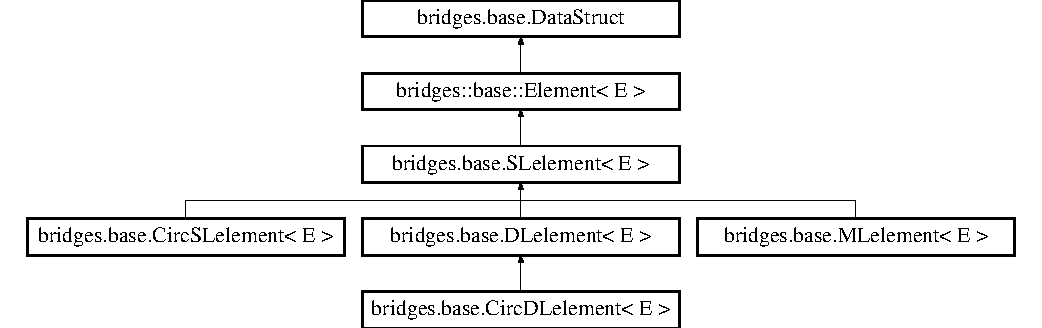
\includegraphics[height=4.000000cm]{classbridges_1_1base_1_1_s_lelement}
\end{center}
\end{figure}
\subsection*{Public Member Functions}
\begin{DoxyCompactItemize}
\item 
\hyperlink{classbridges_1_1base_1_1_s_lelement_ab9c8a08dadd76d7e0c29d7c41cf277c4}{S\+Lelement} ()
\item 
\hyperlink{classbridges_1_1base_1_1_s_lelement_a8e32c9b9e8fc8f9f1eccb14b97e031e7}{S\+Lelement} (String label, E e)
\item 
\hyperlink{classbridges_1_1base_1_1_s_lelement_abc5e333fd2f3289eede108175908f97d}{S\+Lelement} (E e, \hyperlink{classbridges_1_1base_1_1_s_lelement}{S\+Lelement}$<$ E $>$ \hyperlink{classbridges_1_1base_1_1_s_lelement_abf61c96a74ad319d561c6952ea388e0e}{next})
\item 
\hyperlink{classbridges_1_1base_1_1_s_lelement_ab5b1c20ba1d1923fad0780052fb51c99}{S\+Lelement} (\hyperlink{classbridges_1_1base_1_1_s_lelement}{S\+Lelement}$<$ E $>$ \hyperlink{classbridges_1_1base_1_1_s_lelement_abf61c96a74ad319d561c6952ea388e0e}{next})
\item 
String \hyperlink{classbridges_1_1base_1_1_s_lelement_a8c48a2d34b238fa0ae7bf2d1ee58ea88}{get\+Data\+Struct\+Type} ()
\item 
\hyperlink{classbridges_1_1base_1_1_s_lelement}{S\+Lelement}$<$ E $>$ \hyperlink{classbridges_1_1base_1_1_s_lelement_a060c4671e05e3f20b16630343393b80d}{get\+Next} ()
\item 
void \hyperlink{classbridges_1_1base_1_1_s_lelement_afdd42f03071b2614822b73729e1a5a1a}{set\+Next} (\hyperlink{classbridges_1_1base_1_1_s_lelement}{S\+Lelement}$<$ E $>$ \hyperlink{classbridges_1_1base_1_1_s_lelement_abf61c96a74ad319d561c6952ea388e0e}{next})
\item 
String \hyperlink{classbridges_1_1base_1_1_s_lelement_af0ec4da5b29d0f5ab6ab38e91cca51f9}{to\+String} ()
\end{DoxyCompactItemize}
\subsection*{Protected Attributes}
\begin{DoxyCompactItemize}
\item 
\hyperlink{classbridges_1_1base_1_1_s_lelement}{S\+Lelement}$<$ E $>$ \hyperlink{classbridges_1_1base_1_1_s_lelement_abf61c96a74ad319d561c6952ea388e0e}{next} =null
\end{DoxyCompactItemize}
\subsection*{Additional Inherited Members}


\subsection{Detailed Description}
This class can be used to instantiate Singly List Elements. 

This class extends \hyperlink{classbridges_1_1base_1_1_element}{Element} and takes a generic parameter $<$\+E$>$ for representing application specific data.

\begin{DoxyAuthor}{Author}
Mihai Mehedint, Kalpathi Subramanian
\end{DoxyAuthor}

\begin{DoxyParams}{Parameters}
{\em $<$\+E$>$} & \\
\hline
\end{DoxyParams}


\subsection{Constructor \& Destructor Documentation}
\hypertarget{classbridges_1_1base_1_1_s_lelement_ab9c8a08dadd76d7e0c29d7c41cf277c4}{}\label{classbridges_1_1base_1_1_s_lelement_ab9c8a08dadd76d7e0c29d7c41cf277c4} 
\index{bridges\+::base\+::\+S\+Lelement@{bridges\+::base\+::\+S\+Lelement}!S\+Lelement@{S\+Lelement}}
\index{S\+Lelement@{S\+Lelement}!bridges\+::base\+::\+S\+Lelement@{bridges\+::base\+::\+S\+Lelement}}
\subsubsection{\texorpdfstring{S\+Lelement()}{SLelement()}\hspace{0.1cm}{\footnotesize\ttfamily [1/4]}}
{\footnotesize\ttfamily \hyperlink{classbridges_1_1base_1_1_s_lelement}{bridges.\+base.\+S\+Lelement}$<$ E $>$.\hyperlink{classbridges_1_1base_1_1_s_lelement}{S\+Lelement} (\begin{DoxyParamCaption}{ }\end{DoxyParamCaption})}

This constructor creates an \hyperlink{classbridges_1_1base_1_1_s_lelement}{S\+Lelement} object and sets the next pointer to null \hypertarget{classbridges_1_1base_1_1_s_lelement_a8e32c9b9e8fc8f9f1eccb14b97e031e7}{}\label{classbridges_1_1base_1_1_s_lelement_a8e32c9b9e8fc8f9f1eccb14b97e031e7} 
\index{bridges\+::base\+::\+S\+Lelement@{bridges\+::base\+::\+S\+Lelement}!S\+Lelement@{S\+Lelement}}
\index{S\+Lelement@{S\+Lelement}!bridges\+::base\+::\+S\+Lelement@{bridges\+::base\+::\+S\+Lelement}}
\subsubsection{\texorpdfstring{S\+Lelement()}{SLelement()}\hspace{0.1cm}{\footnotesize\ttfamily [2/4]}}
{\footnotesize\ttfamily \hyperlink{classbridges_1_1base_1_1_s_lelement}{bridges.\+base.\+S\+Lelement}$<$ E $>$.\hyperlink{classbridges_1_1base_1_1_s_lelement}{S\+Lelement} (\begin{DoxyParamCaption}\item[{String}]{label,  }\item[{E}]{e }\end{DoxyParamCaption})}

This constructor creates an \hyperlink{classbridges_1_1base_1_1_s_lelement}{S\+Lelement} object of value \char`\"{}e\char`\"{} and label \char`\"{}label\char`\"{} and sets the next pointer to null 
\begin{DoxyParams}{Parameters}
{\em label} & the label of \hyperlink{classbridges_1_1base_1_1_s_lelement}{S\+Lelement} that shows up on the Bridges visualization \\
\hline
{\em e} & the generic object that this \hyperlink{classbridges_1_1base_1_1_s_lelement}{S\+Lelement} will hold \\
\hline
\end{DoxyParams}
\hypertarget{classbridges_1_1base_1_1_s_lelement_abc5e333fd2f3289eede108175908f97d}{}\label{classbridges_1_1base_1_1_s_lelement_abc5e333fd2f3289eede108175908f97d} 
\index{bridges\+::base\+::\+S\+Lelement@{bridges\+::base\+::\+S\+Lelement}!S\+Lelement@{S\+Lelement}}
\index{S\+Lelement@{S\+Lelement}!bridges\+::base\+::\+S\+Lelement@{bridges\+::base\+::\+S\+Lelement}}
\subsubsection{\texorpdfstring{S\+Lelement()}{SLelement()}\hspace{0.1cm}{\footnotesize\ttfamily [3/4]}}
{\footnotesize\ttfamily \hyperlink{classbridges_1_1base_1_1_s_lelement}{bridges.\+base.\+S\+Lelement}$<$ E $>$.\hyperlink{classbridges_1_1base_1_1_s_lelement}{S\+Lelement} (\begin{DoxyParamCaption}\item[{E}]{e,  }\item[{\hyperlink{classbridges_1_1base_1_1_s_lelement}{S\+Lelement}$<$ E $>$}]{next }\end{DoxyParamCaption})}

Creates a new element with value \char`\"{}e\char`\"{} and sets the next pointer to the \hyperlink{classbridges_1_1base_1_1_s_lelement}{S\+Lelement} referenced by the \char`\"{}next\char`\"{} argument 
\begin{DoxyParams}{Parameters}
{\em e} & the generic object that this \hyperlink{classbridges_1_1base_1_1_s_lelement}{S\+Lelement} will hold \\
\hline
{\em next} & the \hyperlink{classbridges_1_1base_1_1_s_lelement}{S\+Lelement} that should be assigned to the next pointer \\
\hline
\end{DoxyParams}
\hypertarget{classbridges_1_1base_1_1_s_lelement_ab5b1c20ba1d1923fad0780052fb51c99}{}\label{classbridges_1_1base_1_1_s_lelement_ab5b1c20ba1d1923fad0780052fb51c99} 
\index{bridges\+::base\+::\+S\+Lelement@{bridges\+::base\+::\+S\+Lelement}!S\+Lelement@{S\+Lelement}}
\index{S\+Lelement@{S\+Lelement}!bridges\+::base\+::\+S\+Lelement@{bridges\+::base\+::\+S\+Lelement}}
\subsubsection{\texorpdfstring{S\+Lelement()}{SLelement()}\hspace{0.1cm}{\footnotesize\ttfamily [4/4]}}
{\footnotesize\ttfamily \hyperlink{classbridges_1_1base_1_1_s_lelement}{bridges.\+base.\+S\+Lelement}$<$ E $>$.\hyperlink{classbridges_1_1base_1_1_s_lelement}{S\+Lelement} (\begin{DoxyParamCaption}\item[{\hyperlink{classbridges_1_1base_1_1_s_lelement}{S\+Lelement}$<$ E $>$}]{next }\end{DoxyParamCaption})}

Creates a new element and sets the next pointer to the \hyperlink{classbridges_1_1base_1_1_s_lelement}{S\+Lelement} \char`\"{}next\char`\"{} 
\begin{DoxyParams}{Parameters}
{\em next} & the \hyperlink{classbridges_1_1base_1_1_s_lelement}{S\+Lelement} that should be assigned to the next pointer \\
\hline
\end{DoxyParams}


\subsection{Member Function Documentation}
\hypertarget{classbridges_1_1base_1_1_s_lelement_a8c48a2d34b238fa0ae7bf2d1ee58ea88}{}\label{classbridges_1_1base_1_1_s_lelement_a8c48a2d34b238fa0ae7bf2d1ee58ea88} 
\index{bridges\+::base\+::\+S\+Lelement@{bridges\+::base\+::\+S\+Lelement}!get\+Data\+Struct\+Type@{get\+Data\+Struct\+Type}}
\index{get\+Data\+Struct\+Type@{get\+Data\+Struct\+Type}!bridges\+::base\+::\+S\+Lelement@{bridges\+::base\+::\+S\+Lelement}}
\subsubsection{\texorpdfstring{get\+Data\+Struct\+Type()}{getDataStructType()}}
{\footnotesize\ttfamily String \hyperlink{classbridges_1_1base_1_1_s_lelement}{bridges.\+base.\+S\+Lelement}$<$ E $>$.get\+Data\+Struct\+Type (\begin{DoxyParamCaption}{ }\end{DoxyParamCaption})}

This method gets the data structure type

\begin{DoxyReturn}{Returns}
The date structure type as a string 
\end{DoxyReturn}
\hypertarget{classbridges_1_1base_1_1_s_lelement_a060c4671e05e3f20b16630343393b80d}{}\label{classbridges_1_1base_1_1_s_lelement_a060c4671e05e3f20b16630343393b80d} 
\index{bridges\+::base\+::\+S\+Lelement@{bridges\+::base\+::\+S\+Lelement}!get\+Next@{get\+Next}}
\index{get\+Next@{get\+Next}!bridges\+::base\+::\+S\+Lelement@{bridges\+::base\+::\+S\+Lelement}}
\subsubsection{\texorpdfstring{get\+Next()}{getNext()}}
{\footnotesize\ttfamily \hyperlink{classbridges_1_1base_1_1_s_lelement}{S\+Lelement}$<$E$>$ \hyperlink{classbridges_1_1base_1_1_s_lelement}{bridges.\+base.\+S\+Lelement}$<$ E $>$.get\+Next (\begin{DoxyParamCaption}{ }\end{DoxyParamCaption})}

Retrieves the next \hyperlink{classbridges_1_1base_1_1_s_lelement}{S\+Lelement} \begin{DoxyReturn}{Returns}
S\+Lelement$<$\+E$>$ assigned to next 
\end{DoxyReturn}
\hypertarget{classbridges_1_1base_1_1_s_lelement_afdd42f03071b2614822b73729e1a5a1a}{}\label{classbridges_1_1base_1_1_s_lelement_afdd42f03071b2614822b73729e1a5a1a} 
\index{bridges\+::base\+::\+S\+Lelement@{bridges\+::base\+::\+S\+Lelement}!set\+Next@{set\+Next}}
\index{set\+Next@{set\+Next}!bridges\+::base\+::\+S\+Lelement@{bridges\+::base\+::\+S\+Lelement}}
\subsubsection{\texorpdfstring{set\+Next()}{setNext()}}
{\footnotesize\ttfamily void \hyperlink{classbridges_1_1base_1_1_s_lelement}{bridges.\+base.\+S\+Lelement}$<$ E $>$.set\+Next (\begin{DoxyParamCaption}\item[{\hyperlink{classbridges_1_1base_1_1_s_lelement}{S\+Lelement}$<$ E $>$}]{next }\end{DoxyParamCaption})}

Sets the pointer to the next \hyperlink{classbridges_1_1base_1_1_s_lelement}{S\+Lelement} 
\begin{DoxyParams}{Parameters}
{\em next} & S\+Lelement$<$\+E$>$ that should be assigned to the next pointer \\
\hline
\end{DoxyParams}
\hypertarget{classbridges_1_1base_1_1_s_lelement_af0ec4da5b29d0f5ab6ab38e91cca51f9}{}\label{classbridges_1_1base_1_1_s_lelement_af0ec4da5b29d0f5ab6ab38e91cca51f9} 
\index{bridges\+::base\+::\+S\+Lelement@{bridges\+::base\+::\+S\+Lelement}!to\+String@{to\+String}}
\index{to\+String@{to\+String}!bridges\+::base\+::\+S\+Lelement@{bridges\+::base\+::\+S\+Lelement}}
\subsubsection{\texorpdfstring{to\+String()}{toString()}}
{\footnotesize\ttfamily String \hyperlink{classbridges_1_1base_1_1_s_lelement}{bridges.\+base.\+S\+Lelement}$<$ E $>$.to\+String (\begin{DoxyParamCaption}{ }\end{DoxyParamCaption})}



\subsection{Member Data Documentation}
\hypertarget{classbridges_1_1base_1_1_s_lelement_abf61c96a74ad319d561c6952ea388e0e}{}\label{classbridges_1_1base_1_1_s_lelement_abf61c96a74ad319d561c6952ea388e0e} 
\index{bridges\+::base\+::\+S\+Lelement@{bridges\+::base\+::\+S\+Lelement}!next@{next}}
\index{next@{next}!bridges\+::base\+::\+S\+Lelement@{bridges\+::base\+::\+S\+Lelement}}
\subsubsection{\texorpdfstring{next}{next}}
{\footnotesize\ttfamily \hyperlink{classbridges_1_1base_1_1_s_lelement}{S\+Lelement}$<$E$>$ \hyperlink{classbridges_1_1base_1_1_s_lelement}{bridges.\+base.\+S\+Lelement}$<$ E $>$.next =null\hspace{0.3cm}{\ttfamily [protected]}}



The documentation for this class was generated from the following file\+:\begin{DoxyCompactItemize}
\item 
link/base/\hyperlink{_s_lelement_8java}{S\+Lelement.\+java}\end{DoxyCompactItemize}

\hypertarget{classbridges_1_1data__src__dependent_1_1_song}{}\section{bridges.\+data\+\_\+src\+\_\+dependent.\+Song Class Reference}
\label{classbridges_1_1data__src__dependent_1_1_song}\index{bridges.\+data\+\_\+src\+\_\+dependent.\+Song@{bridges.\+data\+\_\+src\+\_\+dependent.\+Song}}
\subsection*{Public Member Functions}
\begin{DoxyCompactItemize}
\item 
\hyperlink{classbridges_1_1data__src__dependent_1_1_song_a824052caca0b9c03d07c42e9e7740020}{Song} ()
\item 
\hyperlink{classbridges_1_1data__src__dependent_1_1_song_a78506e63f4d91dc1f0d821050a093ad6}{Song} (String artist, String song, String album, String lyrics, String release\+\_\+date)
\item 
String \hyperlink{classbridges_1_1data__src__dependent_1_1_song_a7aa3685df74e4fbb5e0d4d4750cf7685}{get\+Artist} ()
\item 
void \hyperlink{classbridges_1_1data__src__dependent_1_1_song_adffaec742bf945ec8c81244fdafd47d2}{set\+Artist} (String artist)
\item 
String \hyperlink{classbridges_1_1data__src__dependent_1_1_song_a4e7b8aed1aec243f2798a30e51091d72}{get\+Song\+Title} ()
\item 
void \hyperlink{classbridges_1_1data__src__dependent_1_1_song_a9d7540c0e6cca53ae3a105885aac5622}{set\+Song\+Title} (String song)
\item 
String \hyperlink{classbridges_1_1data__src__dependent_1_1_song_a94b26a355aa1e30938bcc896a8bd902f}{get\+Album\+Title} ()
\item 
void \hyperlink{classbridges_1_1data__src__dependent_1_1_song_ab9f9d24be49c3a0a66c9ff9e271b007e}{set\+Album\+Title} (String album)
\item 
String \hyperlink{classbridges_1_1data__src__dependent_1_1_song_ab4aa2c51f7fdce80d9c178d6f0e0aae8}{get\+Lyrics} ()
\item 
void \hyperlink{classbridges_1_1data__src__dependent_1_1_song_a30889eb971f474e9d62782ddb82c1846}{set\+Lyrics} (String lyrics)
\item 
String \hyperlink{classbridges_1_1data__src__dependent_1_1_song_a05520675a0a2f2e60583887b8c69cde4}{get\+Release\+Date} ()
\item 
void \hyperlink{classbridges_1_1data__src__dependent_1_1_song_a6534e543a295b29858cf98be7a4e276e}{set\+Release\+Date} (String release\+\_\+date)
\end{DoxyCompactItemize}


\subsection{Constructor \& Destructor Documentation}
\mbox{\Hypertarget{classbridges_1_1data__src__dependent_1_1_song_a824052caca0b9c03d07c42e9e7740020}\label{classbridges_1_1data__src__dependent_1_1_song_a824052caca0b9c03d07c42e9e7740020}} 
\index{bridges\+::data\+\_\+src\+\_\+dependent\+::\+Song@{bridges\+::data\+\_\+src\+\_\+dependent\+::\+Song}!Song@{Song}}
\index{Song@{Song}!bridges\+::data\+\_\+src\+\_\+dependent\+::\+Song@{bridges\+::data\+\_\+src\+\_\+dependent\+::\+Song}}
\subsubsection{\texorpdfstring{Song()}{Song()}\hspace{0.1cm}{\footnotesize\ttfamily [1/2]}}
{\footnotesize\ttfamily bridges.\+data\+\_\+src\+\_\+dependent.\+Song.\+Song (\begin{DoxyParamCaption}{ }\end{DoxyParamCaption})}

\hyperlink{classbridges_1_1data__src__dependent_1_1_song}{Song} constructors \mbox{\Hypertarget{classbridges_1_1data__src__dependent_1_1_song_a78506e63f4d91dc1f0d821050a093ad6}\label{classbridges_1_1data__src__dependent_1_1_song_a78506e63f4d91dc1f0d821050a093ad6}} 
\index{bridges\+::data\+\_\+src\+\_\+dependent\+::\+Song@{bridges\+::data\+\_\+src\+\_\+dependent\+::\+Song}!Song@{Song}}
\index{Song@{Song}!bridges\+::data\+\_\+src\+\_\+dependent\+::\+Song@{bridges\+::data\+\_\+src\+\_\+dependent\+::\+Song}}
\subsubsection{\texorpdfstring{Song()}{Song()}\hspace{0.1cm}{\footnotesize\ttfamily [2/2]}}
{\footnotesize\ttfamily bridges.\+data\+\_\+src\+\_\+dependent.\+Song.\+Song (\begin{DoxyParamCaption}\item[{String}]{artist,  }\item[{String}]{song,  }\item[{String}]{album,  }\item[{String}]{lyrics,  }\item[{String}]{release\+\_\+date }\end{DoxyParamCaption})}

\hyperlink{classbridges_1_1data__src__dependent_1_1_song}{Song} constructor


\begin{DoxyParams}{Parameters}
{\em artist} & artist of song \\
\hline
{\em song} & song title \\
\hline
{\em album} & album title \\
\hline
{\em lyrics} & lyrics of song (string) \\
\hline
{\em release\+\_\+date} & date released \\
\hline
\end{DoxyParams}


\subsection{Member Function Documentation}
\mbox{\Hypertarget{classbridges_1_1data__src__dependent_1_1_song_a94b26a355aa1e30938bcc896a8bd902f}\label{classbridges_1_1data__src__dependent_1_1_song_a94b26a355aa1e30938bcc896a8bd902f}} 
\index{bridges\+::data\+\_\+src\+\_\+dependent\+::\+Song@{bridges\+::data\+\_\+src\+\_\+dependent\+::\+Song}!get\+Album\+Title@{get\+Album\+Title}}
\index{get\+Album\+Title@{get\+Album\+Title}!bridges\+::data\+\_\+src\+\_\+dependent\+::\+Song@{bridges\+::data\+\_\+src\+\_\+dependent\+::\+Song}}
\subsubsection{\texorpdfstring{get\+Album\+Title()}{getAlbumTitle()}}
{\footnotesize\ttfamily String bridges.\+data\+\_\+src\+\_\+dependent.\+Song.\+get\+Album\+Title (\begin{DoxyParamCaption}{ }\end{DoxyParamCaption})}

Get album title containing the song \begin{DoxyReturn}{Returns}
album title (string) 
\end{DoxyReturn}
\mbox{\Hypertarget{classbridges_1_1data__src__dependent_1_1_song_a7aa3685df74e4fbb5e0d4d4750cf7685}\label{classbridges_1_1data__src__dependent_1_1_song_a7aa3685df74e4fbb5e0d4d4750cf7685}} 
\index{bridges\+::data\+\_\+src\+\_\+dependent\+::\+Song@{bridges\+::data\+\_\+src\+\_\+dependent\+::\+Song}!get\+Artist@{get\+Artist}}
\index{get\+Artist@{get\+Artist}!bridges\+::data\+\_\+src\+\_\+dependent\+::\+Song@{bridges\+::data\+\_\+src\+\_\+dependent\+::\+Song}}
\subsubsection{\texorpdfstring{get\+Artist()}{getArtist()}}
{\footnotesize\ttfamily String bridges.\+data\+\_\+src\+\_\+dependent.\+Song.\+get\+Artist (\begin{DoxyParamCaption}{ }\end{DoxyParamCaption})}

Get song artist \begin{DoxyReturn}{Returns}
artist of song 
\end{DoxyReturn}
\mbox{\Hypertarget{classbridges_1_1data__src__dependent_1_1_song_ab4aa2c51f7fdce80d9c178d6f0e0aae8}\label{classbridges_1_1data__src__dependent_1_1_song_ab4aa2c51f7fdce80d9c178d6f0e0aae8}} 
\index{bridges\+::data\+\_\+src\+\_\+dependent\+::\+Song@{bridges\+::data\+\_\+src\+\_\+dependent\+::\+Song}!get\+Lyrics@{get\+Lyrics}}
\index{get\+Lyrics@{get\+Lyrics}!bridges\+::data\+\_\+src\+\_\+dependent\+::\+Song@{bridges\+::data\+\_\+src\+\_\+dependent\+::\+Song}}
\subsubsection{\texorpdfstring{get\+Lyrics()}{getLyrics()}}
{\footnotesize\ttfamily String bridges.\+data\+\_\+src\+\_\+dependent.\+Song.\+get\+Lyrics (\begin{DoxyParamCaption}{ }\end{DoxyParamCaption})}

Get lyrics of the song \begin{DoxyReturn}{Returns}
lyrics of song (string) 
\end{DoxyReturn}
\mbox{\Hypertarget{classbridges_1_1data__src__dependent_1_1_song_a05520675a0a2f2e60583887b8c69cde4}\label{classbridges_1_1data__src__dependent_1_1_song_a05520675a0a2f2e60583887b8c69cde4}} 
\index{bridges\+::data\+\_\+src\+\_\+dependent\+::\+Song@{bridges\+::data\+\_\+src\+\_\+dependent\+::\+Song}!get\+Release\+Date@{get\+Release\+Date}}
\index{get\+Release\+Date@{get\+Release\+Date}!bridges\+::data\+\_\+src\+\_\+dependent\+::\+Song@{bridges\+::data\+\_\+src\+\_\+dependent\+::\+Song}}
\subsubsection{\texorpdfstring{get\+Release\+Date()}{getReleaseDate()}}
{\footnotesize\ttfamily String bridges.\+data\+\_\+src\+\_\+dependent.\+Song.\+get\+Release\+Date (\begin{DoxyParamCaption}{ }\end{DoxyParamCaption})}

Get release date of the song \begin{DoxyReturn}{Returns}
release date of song (string) 
\end{DoxyReturn}
\mbox{\Hypertarget{classbridges_1_1data__src__dependent_1_1_song_a4e7b8aed1aec243f2798a30e51091d72}\label{classbridges_1_1data__src__dependent_1_1_song_a4e7b8aed1aec243f2798a30e51091d72}} 
\index{bridges\+::data\+\_\+src\+\_\+dependent\+::\+Song@{bridges\+::data\+\_\+src\+\_\+dependent\+::\+Song}!get\+Song\+Title@{get\+Song\+Title}}
\index{get\+Song\+Title@{get\+Song\+Title}!bridges\+::data\+\_\+src\+\_\+dependent\+::\+Song@{bridges\+::data\+\_\+src\+\_\+dependent\+::\+Song}}
\subsubsection{\texorpdfstring{get\+Song\+Title()}{getSongTitle()}}
{\footnotesize\ttfamily String bridges.\+data\+\_\+src\+\_\+dependent.\+Song.\+get\+Song\+Title (\begin{DoxyParamCaption}{ }\end{DoxyParamCaption})}

Get song title \begin{DoxyReturn}{Returns}
title of song (string) 
\end{DoxyReturn}
\mbox{\Hypertarget{classbridges_1_1data__src__dependent_1_1_song_ab9f9d24be49c3a0a66c9ff9e271b007e}\label{classbridges_1_1data__src__dependent_1_1_song_ab9f9d24be49c3a0a66c9ff9e271b007e}} 
\index{bridges\+::data\+\_\+src\+\_\+dependent\+::\+Song@{bridges\+::data\+\_\+src\+\_\+dependent\+::\+Song}!set\+Album\+Title@{set\+Album\+Title}}
\index{set\+Album\+Title@{set\+Album\+Title}!bridges\+::data\+\_\+src\+\_\+dependent\+::\+Song@{bridges\+::data\+\_\+src\+\_\+dependent\+::\+Song}}
\subsubsection{\texorpdfstring{set\+Album\+Title()}{setAlbumTitle()}}
{\footnotesize\ttfamily void bridges.\+data\+\_\+src\+\_\+dependent.\+Song.\+set\+Album\+Title (\begin{DoxyParamCaption}\item[{String}]{album }\end{DoxyParamCaption})}

Set song album 
\begin{DoxyParams}{Parameters}
{\em album} & song album to set \\
\hline
\end{DoxyParams}
\mbox{\Hypertarget{classbridges_1_1data__src__dependent_1_1_song_adffaec742bf945ec8c81244fdafd47d2}\label{classbridges_1_1data__src__dependent_1_1_song_adffaec742bf945ec8c81244fdafd47d2}} 
\index{bridges\+::data\+\_\+src\+\_\+dependent\+::\+Song@{bridges\+::data\+\_\+src\+\_\+dependent\+::\+Song}!set\+Artist@{set\+Artist}}
\index{set\+Artist@{set\+Artist}!bridges\+::data\+\_\+src\+\_\+dependent\+::\+Song@{bridges\+::data\+\_\+src\+\_\+dependent\+::\+Song}}
\subsubsection{\texorpdfstring{set\+Artist()}{setArtist()}}
{\footnotesize\ttfamily void bridges.\+data\+\_\+src\+\_\+dependent.\+Song.\+set\+Artist (\begin{DoxyParamCaption}\item[{String}]{artist }\end{DoxyParamCaption})}

Set song artist 
\begin{DoxyParams}{Parameters}
{\em artist} & artist to set \\
\hline
\end{DoxyParams}
\mbox{\Hypertarget{classbridges_1_1data__src__dependent_1_1_song_a30889eb971f474e9d62782ddb82c1846}\label{classbridges_1_1data__src__dependent_1_1_song_a30889eb971f474e9d62782ddb82c1846}} 
\index{bridges\+::data\+\_\+src\+\_\+dependent\+::\+Song@{bridges\+::data\+\_\+src\+\_\+dependent\+::\+Song}!set\+Lyrics@{set\+Lyrics}}
\index{set\+Lyrics@{set\+Lyrics}!bridges\+::data\+\_\+src\+\_\+dependent\+::\+Song@{bridges\+::data\+\_\+src\+\_\+dependent\+::\+Song}}
\subsubsection{\texorpdfstring{set\+Lyrics()}{setLyrics()}}
{\footnotesize\ttfamily void bridges.\+data\+\_\+src\+\_\+dependent.\+Song.\+set\+Lyrics (\begin{DoxyParamCaption}\item[{String}]{lyrics }\end{DoxyParamCaption})}

Set song lyrics 
\begin{DoxyParams}{Parameters}
{\em lyrics} & of song to set \\
\hline
\end{DoxyParams}
\mbox{\Hypertarget{classbridges_1_1data__src__dependent_1_1_song_a6534e543a295b29858cf98be7a4e276e}\label{classbridges_1_1data__src__dependent_1_1_song_a6534e543a295b29858cf98be7a4e276e}} 
\index{bridges\+::data\+\_\+src\+\_\+dependent\+::\+Song@{bridges\+::data\+\_\+src\+\_\+dependent\+::\+Song}!set\+Release\+Date@{set\+Release\+Date}}
\index{set\+Release\+Date@{set\+Release\+Date}!bridges\+::data\+\_\+src\+\_\+dependent\+::\+Song@{bridges\+::data\+\_\+src\+\_\+dependent\+::\+Song}}
\subsubsection{\texorpdfstring{set\+Release\+Date()}{setReleaseDate()}}
{\footnotesize\ttfamily void bridges.\+data\+\_\+src\+\_\+dependent.\+Song.\+set\+Release\+Date (\begin{DoxyParamCaption}\item[{String}]{release\+\_\+date }\end{DoxyParamCaption})}

Set release date of song 
\begin{DoxyParams}{Parameters}
{\em release\+\_\+date} & date of release to set \\
\hline
\end{DoxyParams}
\mbox{\Hypertarget{classbridges_1_1data__src__dependent_1_1_song_a9d7540c0e6cca53ae3a105885aac5622}\label{classbridges_1_1data__src__dependent_1_1_song_a9d7540c0e6cca53ae3a105885aac5622}} 
\index{bridges\+::data\+\_\+src\+\_\+dependent\+::\+Song@{bridges\+::data\+\_\+src\+\_\+dependent\+::\+Song}!set\+Song\+Title@{set\+Song\+Title}}
\index{set\+Song\+Title@{set\+Song\+Title}!bridges\+::data\+\_\+src\+\_\+dependent\+::\+Song@{bridges\+::data\+\_\+src\+\_\+dependent\+::\+Song}}
\subsubsection{\texorpdfstring{set\+Song\+Title()}{setSongTitle()}}
{\footnotesize\ttfamily void bridges.\+data\+\_\+src\+\_\+dependent.\+Song.\+set\+Song\+Title (\begin{DoxyParamCaption}\item[{String}]{song }\end{DoxyParamCaption})}

Set song title 
\begin{DoxyParams}{Parameters}
{\em song} & song title to set \\
\hline
\end{DoxyParams}


The documentation for this class was generated from the following file\+:\begin{DoxyCompactItemize}
\item 
/home/erik/work/bridges/bridges-\/java/src/main/java/bridges/data\+\_\+src\+\_\+dependent/\hyperlink{_song_8java}{Song.\+java}\end{DoxyCompactItemize}

\hypertarget{classbridges_1_1base_1_1_tree_element}{}\section{bridges.\+base.\+Tree\+Element$<$ E $>$ Class Template Reference}
\label{classbridges_1_1base_1_1_tree_element}\index{bridges.base.TreeElement$<$ E $>$@{bridges.base.TreeElement$<$ E $>$}}


This class extends \mbox{\hyperlink{classbridges_1_1base_1_1_element}{Element}} to represent general trees with arbitrary number of children.  


Inheritance diagram for bridges.\+base.\+Tree\+Element$<$ E $>$\+:\begin{figure}[H]
\begin{center}
\leavevmode
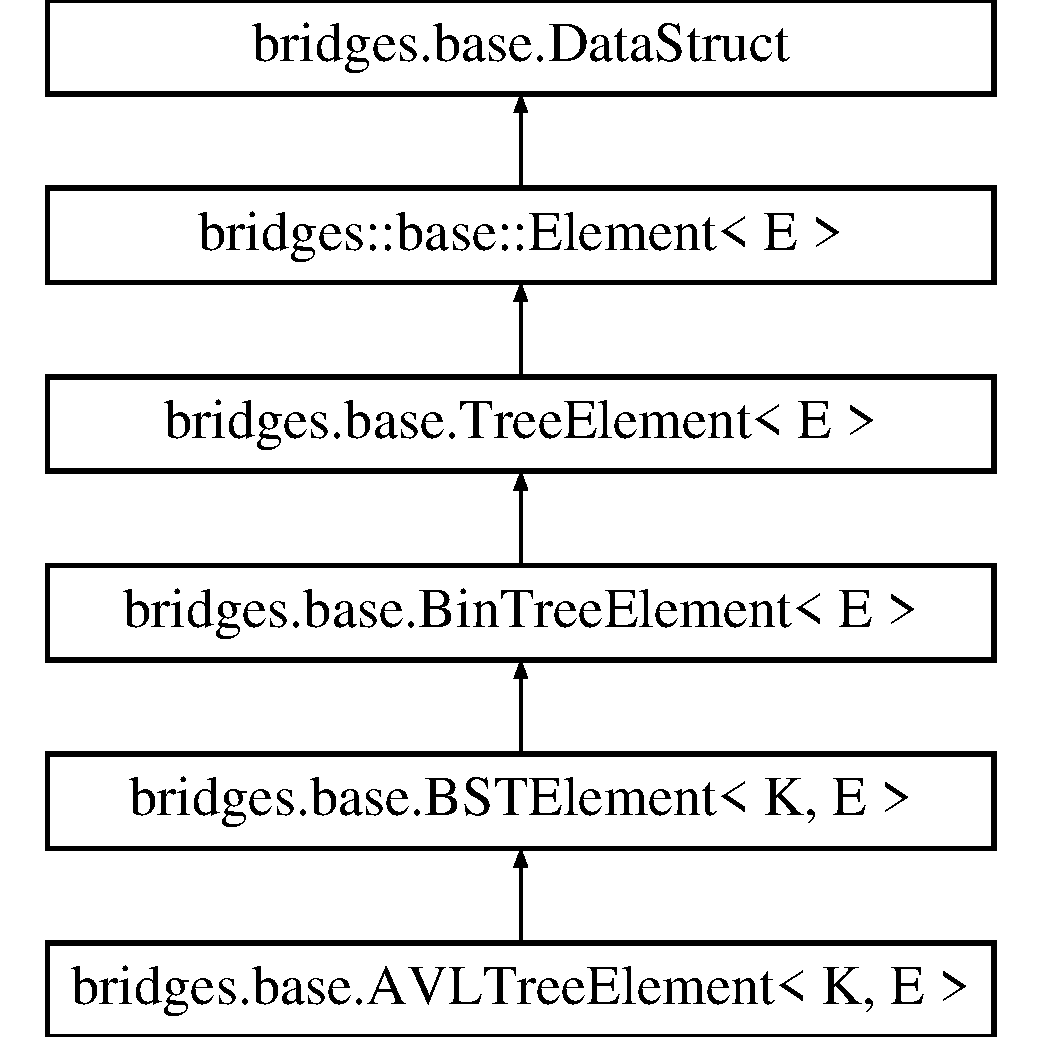
\includegraphics[height=6.000000cm]{classbridges_1_1base_1_1_tree_element}
\end{center}
\end{figure}
\subsection*{Public Member Functions}
\begin{DoxyCompactItemize}
\item 
\mbox{\hyperlink{classbridges_1_1base_1_1_tree_element_ab1af682e9304f5427e308ba5f43d7a9a}{Tree\+Element}} ()
\item 
\mbox{\hyperlink{classbridges_1_1base_1_1_tree_element_a0f17c278536239fb6cba051246ef67a8}{Tree\+Element}} (E e)
\item 
\mbox{\hyperlink{classbridges_1_1base_1_1_tree_element_a476cbeedf2c56f6a40a632035b7d740e}{Tree\+Element}} (String label, E e)
\item 
\mbox{\hyperlink{classbridges_1_1base_1_1_tree_element_aae24dfde287dc0596c69ad853f12f72e}{Tree\+Element}} (\mbox{\hyperlink{classbridges_1_1base_1_1_tree_element}{Tree\+Element}}$<$ E $>$ left, \mbox{\hyperlink{classbridges_1_1base_1_1_tree_element}{Tree\+Element}}$<$ E $>$ right)
\item 
\mbox{\hyperlink{classbridges_1_1base_1_1_tree_element_ace86faa0e65626833c61cc8418cfb1ed}{Tree\+Element}} (E e, \mbox{\hyperlink{classbridges_1_1base_1_1_tree_element}{Tree\+Element}}$<$ E $>$ left, \mbox{\hyperlink{classbridges_1_1base_1_1_tree_element}{Tree\+Element}}$<$ E $>$ right)
\item 
String \mbox{\hyperlink{classbridges_1_1base_1_1_tree_element_a5e0d5f8991d72bd7b0e76d6b0b8662a7}{get\+Data\+Struct\+Type}} ()
\item 
void \mbox{\hyperlink{classbridges_1_1base_1_1_tree_element_a473c29486e99edc725423941b203e939}{add\+Child}} (\mbox{\hyperlink{classbridges_1_1base_1_1_tree_element}{Tree\+Element}}$<$ E $>$ child)
\item 
int \mbox{\hyperlink{classbridges_1_1base_1_1_tree_element_a3722c7cec66ff297f999870df0da3cff}{get\+Number\+Of\+Children}} ()
\item 
void \mbox{\hyperlink{classbridges_1_1base_1_1_tree_element_aefafebb19d64398d150e464e4361ddf0}{set\+Child}} (int index, \mbox{\hyperlink{classbridges_1_1base_1_1_tree_element}{Tree\+Element}}$<$ E $>$ child)
\item 
\mbox{\hyperlink{classbridges_1_1base_1_1_tree_element}{Tree\+Element}}$<$ E $>$ \mbox{\hyperlink{classbridges_1_1base_1_1_tree_element_a4ee40d69ce52fdcac321554564d10aa3}{get\+Child}} (int index)
\item 
String \mbox{\hyperlink{classbridges_1_1base_1_1_tree_element_a674870c91b39fac88d35a569fd505e9b}{get\+Data\+Structure\+Representation}} ()
\end{DoxyCompactItemize}
\subsection*{Additional Inherited Members}


\subsection{Detailed Description}
This class extends \mbox{\hyperlink{classbridges_1_1base_1_1_element}{Element}} to represent general trees with arbitrary number of children. 

\mbox{\hyperlink{classbridges_1_1base_1_1_tree_element}{Tree\+Element}} nodes can have an arbitrary number of child nodes(held in in a vector in the order in which they were added). The visualization of trees assumes that the children are drawn in order from left to right.

Tree Elements have labels (string) that are displayed on the visualization. Elements take an generic object E as a user defined parameter, which can be any native type or object.

Elements contain a visualizer (\mbox{\hyperlink{classbridges_1_1base_1_1_element_visualizer}{Element\+Visualizer}}) object for setting visual attributes (color, shape, opacity, size), necessary for displaying them in a web browser.

Elements also have a \mbox{\hyperlink{classbridges_1_1base_1_1_link_visualizer}{Link\+Visualizer}} object that is used when they are linked to another element, appropriate for setting link attributes, between parent and child nodes.

\begin{DoxyAuthor}{Author}
Kalpathi Subramanian
\end{DoxyAuthor}
\begin{DoxyDate}{Date}
6/22/16, 5/17/17
\end{DoxyDate}

\begin{DoxyParams}{Parameters}
{\em $<$\+E$>$} & The generic parameter object that is part of this element, representing application specific data.\\
\hline
\end{DoxyParams}
\begin{DoxySeeAlso}{See also}
Example tutorial at ~\newline
 ?? 
\end{DoxySeeAlso}


\subsection{Constructor \& Destructor Documentation}
\mbox{\Hypertarget{classbridges_1_1base_1_1_tree_element_ab1af682e9304f5427e308ba5f43d7a9a}\label{classbridges_1_1base_1_1_tree_element_ab1af682e9304f5427e308ba5f43d7a9a}} 
\index{bridges.base.TreeElement$<$ E $>$@{bridges.base.TreeElement$<$ E $>$}!TreeElement@{TreeElement}}
\index{TreeElement@{TreeElement}!bridges.base.TreeElement$<$ E $>$@{bridges.base.TreeElement$<$ E $>$}}
\subsubsection{\texorpdfstring{TreeElement()}{TreeElement()}\hspace{0.1cm}{\footnotesize\ttfamily [1/5]}}
{\footnotesize\ttfamily \mbox{\hyperlink{classbridges_1_1base_1_1_tree_element}{bridges.\+base.\+Tree\+Element}}$<$ E $>$.\mbox{\hyperlink{classbridges_1_1base_1_1_tree_element}{Tree\+Element}} (\begin{DoxyParamCaption}{ }\end{DoxyParamCaption})}

Constructs an empty \mbox{\hyperlink{classbridges_1_1base_1_1_tree_element}{Tree\+Element}} with first two children set to null. \mbox{\Hypertarget{classbridges_1_1base_1_1_tree_element_a0f17c278536239fb6cba051246ef67a8}\label{classbridges_1_1base_1_1_tree_element_a0f17c278536239fb6cba051246ef67a8}} 
\index{bridges.base.TreeElement$<$ E $>$@{bridges.base.TreeElement$<$ E $>$}!TreeElement@{TreeElement}}
\index{TreeElement@{TreeElement}!bridges.base.TreeElement$<$ E $>$@{bridges.base.TreeElement$<$ E $>$}}
\subsubsection{\texorpdfstring{TreeElement()}{TreeElement()}\hspace{0.1cm}{\footnotesize\ttfamily [2/5]}}
{\footnotesize\ttfamily \mbox{\hyperlink{classbridges_1_1base_1_1_tree_element}{bridges.\+base.\+Tree\+Element}}$<$ E $>$.\mbox{\hyperlink{classbridges_1_1base_1_1_tree_element}{Tree\+Element}} (\begin{DoxyParamCaption}\item[{E}]{e }\end{DoxyParamCaption})}

Constructs a \mbox{\hyperlink{classbridges_1_1base_1_1_tree_element}{Tree\+Element}} holding an object \char`\"{}e\char`\"{} with first two children set to null.


\begin{DoxyParams}{Parameters}
{\em e} & the generic object that \mbox{\hyperlink{classbridges_1_1base_1_1_tree_element}{Tree\+Element}} will hold \\
\hline
\end{DoxyParams}
\mbox{\Hypertarget{classbridges_1_1base_1_1_tree_element_a476cbeedf2c56f6a40a632035b7d740e}\label{classbridges_1_1base_1_1_tree_element_a476cbeedf2c56f6a40a632035b7d740e}} 
\index{bridges.base.TreeElement$<$ E $>$@{bridges.base.TreeElement$<$ E $>$}!TreeElement@{TreeElement}}
\index{TreeElement@{TreeElement}!bridges.base.TreeElement$<$ E $>$@{bridges.base.TreeElement$<$ E $>$}}
\subsubsection{\texorpdfstring{TreeElement()}{TreeElement()}\hspace{0.1cm}{\footnotesize\ttfamily [3/5]}}
{\footnotesize\ttfamily \mbox{\hyperlink{classbridges_1_1base_1_1_tree_element}{bridges.\+base.\+Tree\+Element}}$<$ E $>$.\mbox{\hyperlink{classbridges_1_1base_1_1_tree_element}{Tree\+Element}} (\begin{DoxyParamCaption}\item[{String}]{label,  }\item[{E}]{e }\end{DoxyParamCaption})}

Constructs a \mbox{\hyperlink{classbridges_1_1base_1_1_tree_element}{Tree\+Element}} with label set to \char`\"{}label\char`\"{}, holding an object \char`\"{}e\char`\"{}. 
\begin{DoxyParams}{Parameters}
{\em label} & the label of \mbox{\hyperlink{classbridges_1_1base_1_1_tree_element}{Tree\+Element}} that shows up on the Bridges visualization \\
\hline
{\em e} & the generic object that \mbox{\hyperlink{classbridges_1_1base_1_1_tree_element}{Tree\+Element}} will hold \\
\hline
\end{DoxyParams}
\mbox{\Hypertarget{classbridges_1_1base_1_1_tree_element_aae24dfde287dc0596c69ad853f12f72e}\label{classbridges_1_1base_1_1_tree_element_aae24dfde287dc0596c69ad853f12f72e}} 
\index{bridges.base.TreeElement$<$ E $>$@{bridges.base.TreeElement$<$ E $>$}!TreeElement@{TreeElement}}
\index{TreeElement@{TreeElement}!bridges.base.TreeElement$<$ E $>$@{bridges.base.TreeElement$<$ E $>$}}
\subsubsection{\texorpdfstring{TreeElement()}{TreeElement()}\hspace{0.1cm}{\footnotesize\ttfamily [4/5]}}
{\footnotesize\ttfamily \mbox{\hyperlink{classbridges_1_1base_1_1_tree_element}{bridges.\+base.\+Tree\+Element}}$<$ E $>$.\mbox{\hyperlink{classbridges_1_1base_1_1_tree_element}{Tree\+Element}} (\begin{DoxyParamCaption}\item[{\mbox{\hyperlink{classbridges_1_1base_1_1_tree_element}{Tree\+Element}}$<$ E $>$}]{left,  }\item[{\mbox{\hyperlink{classbridges_1_1base_1_1_tree_element}{Tree\+Element}}$<$ E $>$}]{right }\end{DoxyParamCaption})}

Constructs an empty \mbox{\hyperlink{classbridges_1_1base_1_1_tree_element}{Tree\+Element}} left pointer pointing to child 0 and right pointer pointing to child 1.


\begin{DoxyParams}{Parameters}
{\em left} & the \mbox{\hyperlink{classbridges_1_1base_1_1_tree_element}{Tree\+Element}} to be assigned to the child 0 of this \mbox{\hyperlink{classbridges_1_1base_1_1_tree_element}{Tree\+Element}} \\
\hline
{\em right} & the \mbox{\hyperlink{classbridges_1_1base_1_1_tree_element}{Tree\+Element}} to be assigned to the child 1 of this \mbox{\hyperlink{classbridges_1_1base_1_1_tree_element}{Tree\+Element}} \\
\hline
\end{DoxyParams}
\mbox{\Hypertarget{classbridges_1_1base_1_1_tree_element_ace86faa0e65626833c61cc8418cfb1ed}\label{classbridges_1_1base_1_1_tree_element_ace86faa0e65626833c61cc8418cfb1ed}} 
\index{bridges.base.TreeElement$<$ E $>$@{bridges.base.TreeElement$<$ E $>$}!TreeElement@{TreeElement}}
\index{TreeElement@{TreeElement}!bridges.base.TreeElement$<$ E $>$@{bridges.base.TreeElement$<$ E $>$}}
\subsubsection{\texorpdfstring{TreeElement()}{TreeElement()}\hspace{0.1cm}{\footnotesize\ttfamily [5/5]}}
{\footnotesize\ttfamily \mbox{\hyperlink{classbridges_1_1base_1_1_tree_element}{bridges.\+base.\+Tree\+Element}}$<$ E $>$.\mbox{\hyperlink{classbridges_1_1base_1_1_tree_element}{Tree\+Element}} (\begin{DoxyParamCaption}\item[{E}]{e,  }\item[{\mbox{\hyperlink{classbridges_1_1base_1_1_tree_element}{Tree\+Element}}$<$ E $>$}]{left,  }\item[{\mbox{\hyperlink{classbridges_1_1base_1_1_tree_element}{Tree\+Element}}$<$ E $>$}]{right }\end{DoxyParamCaption})}

Constructs a \mbox{\hyperlink{classbridges_1_1base_1_1_tree_element}{Tree\+Element}} holding the object \char`\"{}e\char`\"{}, left pointer pointing to first child and right pointer pointing to second child


\begin{DoxyParams}{Parameters}
{\em e} & the generic object that \mbox{\hyperlink{classbridges_1_1base_1_1_tree_element}{Tree\+Element}} will hold \\
\hline
{\em left} & the \mbox{\hyperlink{classbridges_1_1base_1_1_tree_element}{Tree\+Element}} to be assigned to the first child of this \mbox{\hyperlink{classbridges_1_1base_1_1_tree_element}{Tree\+Element}} \\
\hline
{\em right} & the \mbox{\hyperlink{classbridges_1_1base_1_1_tree_element}{Tree\+Element}} to be assigned to the second child of this \mbox{\hyperlink{classbridges_1_1base_1_1_tree_element}{Tree\+Element}} \\
\hline
\end{DoxyParams}


\subsection{Member Function Documentation}
\mbox{\Hypertarget{classbridges_1_1base_1_1_tree_element_a473c29486e99edc725423941b203e939}\label{classbridges_1_1base_1_1_tree_element_a473c29486e99edc725423941b203e939}} 
\index{bridges.base.TreeElement$<$ E $>$@{bridges.base.TreeElement$<$ E $>$}!addChild@{addChild}}
\index{addChild@{addChild}!bridges.base.TreeElement$<$ E $>$@{bridges.base.TreeElement$<$ E $>$}}
\subsubsection{\texorpdfstring{addChild()}{addChild()}}
{\footnotesize\ttfamily void \mbox{\hyperlink{classbridges_1_1base_1_1_tree_element}{bridges.\+base.\+Tree\+Element}}$<$ E $>$.add\+Child (\begin{DoxyParamCaption}\item[{\mbox{\hyperlink{classbridges_1_1base_1_1_tree_element}{Tree\+Element}}$<$ E $>$}]{child }\end{DoxyParamCaption})}

Adds a child to the node \mbox{\Hypertarget{classbridges_1_1base_1_1_tree_element_a4ee40d69ce52fdcac321554564d10aa3}\label{classbridges_1_1base_1_1_tree_element_a4ee40d69ce52fdcac321554564d10aa3}} 
\index{bridges.base.TreeElement$<$ E $>$@{bridges.base.TreeElement$<$ E $>$}!getChild@{getChild}}
\index{getChild@{getChild}!bridges.base.TreeElement$<$ E $>$@{bridges.base.TreeElement$<$ E $>$}}
\subsubsection{\texorpdfstring{getChild()}{getChild()}}
{\footnotesize\ttfamily \mbox{\hyperlink{classbridges_1_1base_1_1_tree_element}{Tree\+Element}}$<$E$>$ \mbox{\hyperlink{classbridges_1_1base_1_1_tree_element}{bridges.\+base.\+Tree\+Element}}$<$ E $>$.get\+Child (\begin{DoxyParamCaption}\item[{int}]{index }\end{DoxyParamCaption})}

gets a child at a particular index


\begin{DoxyParams}{Parameters}
{\em index} & into the list of children\\
\hline
\end{DoxyParams}
\begin{DoxyReturn}{Returns}
child to be returned 
\end{DoxyReturn}
\mbox{\Hypertarget{classbridges_1_1base_1_1_tree_element_a5e0d5f8991d72bd7b0e76d6b0b8662a7}\label{classbridges_1_1base_1_1_tree_element_a5e0d5f8991d72bd7b0e76d6b0b8662a7}} 
\index{bridges.base.TreeElement$<$ E $>$@{bridges.base.TreeElement$<$ E $>$}!getDataStructType@{getDataStructType}}
\index{getDataStructType@{getDataStructType}!bridges.base.TreeElement$<$ E $>$@{bridges.base.TreeElement$<$ E $>$}}
\subsubsection{\texorpdfstring{getDataStructType()}{getDataStructType()}}
{\footnotesize\ttfamily String \mbox{\hyperlink{classbridges_1_1base_1_1_tree_element}{bridges.\+base.\+Tree\+Element}}$<$ E $>$.get\+Data\+Struct\+Type (\begin{DoxyParamCaption}{ }\end{DoxyParamCaption})}

This method gets the data structure type

\begin{DoxyReturn}{Returns}
The date structure type as a string 
\end{DoxyReturn}
\mbox{\Hypertarget{classbridges_1_1base_1_1_tree_element_a674870c91b39fac88d35a569fd505e9b}\label{classbridges_1_1base_1_1_tree_element_a674870c91b39fac88d35a569fd505e9b}} 
\index{bridges.base.TreeElement$<$ E $>$@{bridges.base.TreeElement$<$ E $>$}!getDataStructureRepresentation@{getDataStructureRepresentation}}
\index{getDataStructureRepresentation@{getDataStructureRepresentation}!bridges.base.TreeElement$<$ E $>$@{bridges.base.TreeElement$<$ E $>$}}
\subsubsection{\texorpdfstring{getDataStructureRepresentation()}{getDataStructureRepresentation()}}
{\footnotesize\ttfamily String \mbox{\hyperlink{classbridges_1_1base_1_1_tree_element}{bridges.\+base.\+Tree\+Element}}$<$ E $>$.get\+Data\+Structure\+Representation (\begin{DoxyParamCaption}{ }\end{DoxyParamCaption})}

Get hierarchical J\+S\+ON of the tree representation

\begin{DoxyReturn}{Returns}
the J\+S\+ON string 
\end{DoxyReturn}
\mbox{\Hypertarget{classbridges_1_1base_1_1_tree_element_a3722c7cec66ff297f999870df0da3cff}\label{classbridges_1_1base_1_1_tree_element_a3722c7cec66ff297f999870df0da3cff}} 
\index{bridges.base.TreeElement$<$ E $>$@{bridges.base.TreeElement$<$ E $>$}!getNumberOfChildren@{getNumberOfChildren}}
\index{getNumberOfChildren@{getNumberOfChildren}!bridges.base.TreeElement$<$ E $>$@{bridges.base.TreeElement$<$ E $>$}}
\subsubsection{\texorpdfstring{getNumberOfChildren()}{getNumberOfChildren()}}
{\footnotesize\ttfamily int \mbox{\hyperlink{classbridges_1_1base_1_1_tree_element}{bridges.\+base.\+Tree\+Element}}$<$ E $>$.get\+Number\+Of\+Children (\begin{DoxyParamCaption}{ }\end{DoxyParamCaption})}

Returns the number of children at this node

\begin{DoxyReturn}{Returns}
number of children 
\end{DoxyReturn}
\mbox{\Hypertarget{classbridges_1_1base_1_1_tree_element_aefafebb19d64398d150e464e4361ddf0}\label{classbridges_1_1base_1_1_tree_element_aefafebb19d64398d150e464e4361ddf0}} 
\index{bridges.base.TreeElement$<$ E $>$@{bridges.base.TreeElement$<$ E $>$}!setChild@{setChild}}
\index{setChild@{setChild}!bridges.base.TreeElement$<$ E $>$@{bridges.base.TreeElement$<$ E $>$}}
\subsubsection{\texorpdfstring{setChild()}{setChild()}}
{\footnotesize\ttfamily void \mbox{\hyperlink{classbridges_1_1base_1_1_tree_element}{bridges.\+base.\+Tree\+Element}}$<$ E $>$.set\+Child (\begin{DoxyParamCaption}\item[{int}]{index,  }\item[{\mbox{\hyperlink{classbridges_1_1base_1_1_tree_element}{Tree\+Element}}$<$ E $>$}]{child }\end{DoxyParamCaption})}

adds a child to the node -\/ will be added at the next open position


\begin{DoxyParams}{Parameters}
{\em child} & to be added\\
\hline
\end{DoxyParams}
\begin{DoxyReturn}{Returns}
none 
\end{DoxyReturn}


The documentation for this class was generated from the following file\+:\begin{DoxyCompactItemize}
\item 
/\+Users/kalpathi/gr/bridges/java/src/main/java/bridges/base/\mbox{\hyperlink{_tree_element_8java}{Tree\+Element.\+java}}\end{DoxyCompactItemize}

\hypertarget{classbridges_1_1data__src__dependent_1_1_tweet}{}\section{bridges.\+data\+\_\+src\+\_\+dependent.\+Tweet Class Reference}
\label{classbridges_1_1data__src__dependent_1_1_tweet}\index{bridges.\+data\+\_\+src\+\_\+dependent.\+Tweet@{bridges.\+data\+\_\+src\+\_\+dependent.\+Tweet}}
Inheritance diagram for bridges.\+data\+\_\+src\+\_\+dependent.\+Tweet\+:\begin{figure}[H]
\begin{center}
\leavevmode
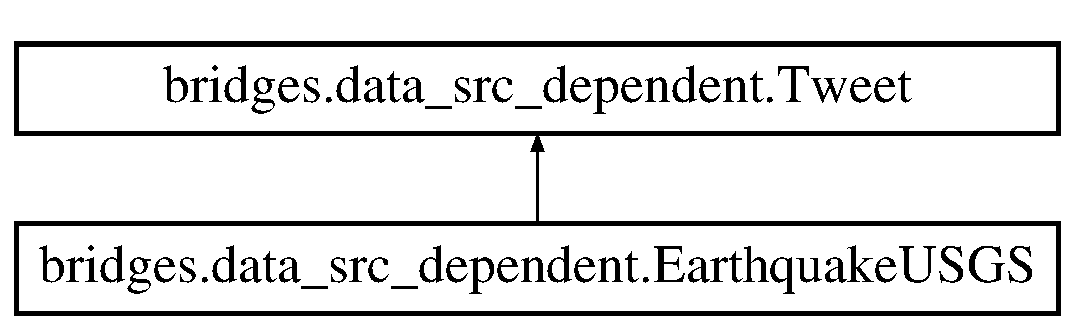
\includegraphics[height=1.992882cm]{classbridges_1_1data__src__dependent_1_1_tweet}
\end{center}
\end{figure}
\subsection*{Public Member Functions}
\begin{DoxyCompactItemize}
\item 
\hyperlink{classbridges_1_1data__src__dependent_1_1_tweet_a615278c2672b2cb310d3c645566ad5cd}{Tweet} (String content, Date date2)
\item 
\hyperlink{classbridges_1_1data__src__dependent_1_1_tweet_a611e969f630c86098b204cfb4655f79b}{Tweet} (String content)
\item 
\hyperlink{classbridges_1_1data__src__dependent_1_1_tweet_a0b0ee5fa9a6221da95020bd5f78667d9}{Tweet} (\hyperlink{classbridges_1_1data__src__dependent_1_1_tweet}{Tweet} a\+Tweet\+To\+Copy)
\item 
String \hyperlink{classbridges_1_1data__src__dependent_1_1_tweet_a9b48f1ffc14fea21eb8a3e742601974a}{get\+Content} ()
\item 
void \hyperlink{classbridges_1_1data__src__dependent_1_1_tweet_a80ac618b5817392ce356657b2bf4145a}{set\+Content} (String content)
\item 
void \hyperlink{classbridges_1_1data__src__dependent_1_1_tweet_aa193633f4f61cc957f05a1c551f18822}{set\+Label} (String label)
\item 
String \hyperlink{classbridges_1_1data__src__dependent_1_1_tweet_a4b31431e42327efa953adde4c15cf168}{get\+Label} ()
\item 
Date \hyperlink{classbridges_1_1data__src__dependent_1_1_tweet_a801b0b5ea0127746c9c8ec0fc5e35ac2}{get\+Date} ()
\item 
void \hyperlink{classbridges_1_1data__src__dependent_1_1_tweet_a1a57c028bb87ad4e94af496a7260ffe9}{set\+Date} (Date date)
\item 
int \hyperlink{classbridges_1_1data__src__dependent_1_1_tweet_adf7dadcda59b68bb00b42480e4ad9956}{hash\+Code} ()
\item 
boolean \hyperlink{classbridges_1_1data__src__dependent_1_1_tweet_ae5edb76b9dd0f76b56eb40aa7c8cc077}{equals} (Object obj)
\item 
String \hyperlink{classbridges_1_1data__src__dependent_1_1_tweet_adfba67504a7463a7f16aff46d2bb893f}{to\+String} ()
\end{DoxyCompactItemize}


\subsection{Detailed Description}
\begin{DoxyAuthor}{Author}
Sean Gallager  author mihai mehedint 
\end{DoxyAuthor}


\subsection{Constructor \& Destructor Documentation}
\hypertarget{classbridges_1_1data__src__dependent_1_1_tweet_a615278c2672b2cb310d3c645566ad5cd}{}\index{bridges\+::data\+\_\+src\+\_\+dependent\+::\+Tweet@{bridges\+::data\+\_\+src\+\_\+dependent\+::\+Tweet}!Tweet@{Tweet}}
\index{Tweet@{Tweet}!bridges\+::data\+\_\+src\+\_\+dependent\+::\+Tweet@{bridges\+::data\+\_\+src\+\_\+dependent\+::\+Tweet}}
\subsubsection[{Tweet(\+String content, Date date2)}]{\setlength{\rightskip}{0pt plus 5cm}bridges.\+data\+\_\+src\+\_\+dependent.\+Tweet.\+Tweet (
\begin{DoxyParamCaption}
\item[{String}]{content, }
\item[{Date}]{date2}
\end{DoxyParamCaption}
)}\label{classbridges_1_1data__src__dependent_1_1_tweet_a615278c2672b2cb310d3c645566ad5cd}
\hypertarget{classbridges_1_1data__src__dependent_1_1_tweet_a611e969f630c86098b204cfb4655f79b}{}\index{bridges\+::data\+\_\+src\+\_\+dependent\+::\+Tweet@{bridges\+::data\+\_\+src\+\_\+dependent\+::\+Tweet}!Tweet@{Tweet}}
\index{Tweet@{Tweet}!bridges\+::data\+\_\+src\+\_\+dependent\+::\+Tweet@{bridges\+::data\+\_\+src\+\_\+dependent\+::\+Tweet}}
\subsubsection[{Tweet(\+String content)}]{\setlength{\rightskip}{0pt plus 5cm}bridges.\+data\+\_\+src\+\_\+dependent.\+Tweet.\+Tweet (
\begin{DoxyParamCaption}
\item[{String}]{content}
\end{DoxyParamCaption}
)}\label{classbridges_1_1data__src__dependent_1_1_tweet_a611e969f630c86098b204cfb4655f79b}
\hypertarget{classbridges_1_1data__src__dependent_1_1_tweet_a0b0ee5fa9a6221da95020bd5f78667d9}{}\index{bridges\+::data\+\_\+src\+\_\+dependent\+::\+Tweet@{bridges\+::data\+\_\+src\+\_\+dependent\+::\+Tweet}!Tweet@{Tweet}}
\index{Tweet@{Tweet}!bridges\+::data\+\_\+src\+\_\+dependent\+::\+Tweet@{bridges\+::data\+\_\+src\+\_\+dependent\+::\+Tweet}}
\subsubsection[{Tweet(\+Tweet a\+Tweet\+To\+Copy)}]{\setlength{\rightskip}{0pt plus 5cm}bridges.\+data\+\_\+src\+\_\+dependent.\+Tweet.\+Tweet (
\begin{DoxyParamCaption}
\item[{{\bf Tweet}}]{a\+Tweet\+To\+Copy}
\end{DoxyParamCaption}
)}\label{classbridges_1_1data__src__dependent_1_1_tweet_a0b0ee5fa9a6221da95020bd5f78667d9}


\subsection{Member Function Documentation}
\hypertarget{classbridges_1_1data__src__dependent_1_1_tweet_ae5edb76b9dd0f76b56eb40aa7c8cc077}{}\index{bridges\+::data\+\_\+src\+\_\+dependent\+::\+Tweet@{bridges\+::data\+\_\+src\+\_\+dependent\+::\+Tweet}!equals@{equals}}
\index{equals@{equals}!bridges\+::data\+\_\+src\+\_\+dependent\+::\+Tweet@{bridges\+::data\+\_\+src\+\_\+dependent\+::\+Tweet}}
\subsubsection[{equals(\+Object obj)}]{\setlength{\rightskip}{0pt plus 5cm}boolean bridges.\+data\+\_\+src\+\_\+dependent.\+Tweet.\+equals (
\begin{DoxyParamCaption}
\item[{Object}]{obj}
\end{DoxyParamCaption}
)}\label{classbridges_1_1data__src__dependent_1_1_tweet_ae5edb76b9dd0f76b56eb40aa7c8cc077}
\hypertarget{classbridges_1_1data__src__dependent_1_1_tweet_a9b48f1ffc14fea21eb8a3e742601974a}{}\index{bridges\+::data\+\_\+src\+\_\+dependent\+::\+Tweet@{bridges\+::data\+\_\+src\+\_\+dependent\+::\+Tweet}!get\+Content@{get\+Content}}
\index{get\+Content@{get\+Content}!bridges\+::data\+\_\+src\+\_\+dependent\+::\+Tweet@{bridges\+::data\+\_\+src\+\_\+dependent\+::\+Tweet}}
\subsubsection[{get\+Content()}]{\setlength{\rightskip}{0pt plus 5cm}String bridges.\+data\+\_\+src\+\_\+dependent.\+Tweet.\+get\+Content (
\begin{DoxyParamCaption}
{}
\end{DoxyParamCaption}
)}\label{classbridges_1_1data__src__dependent_1_1_tweet_a9b48f1ffc14fea21eb8a3e742601974a}
\hypertarget{classbridges_1_1data__src__dependent_1_1_tweet_a801b0b5ea0127746c9c8ec0fc5e35ac2}{}\index{bridges\+::data\+\_\+src\+\_\+dependent\+::\+Tweet@{bridges\+::data\+\_\+src\+\_\+dependent\+::\+Tweet}!get\+Date@{get\+Date}}
\index{get\+Date@{get\+Date}!bridges\+::data\+\_\+src\+\_\+dependent\+::\+Tweet@{bridges\+::data\+\_\+src\+\_\+dependent\+::\+Tweet}}
\subsubsection[{get\+Date()}]{\setlength{\rightskip}{0pt plus 5cm}Date bridges.\+data\+\_\+src\+\_\+dependent.\+Tweet.\+get\+Date (
\begin{DoxyParamCaption}
{}
\end{DoxyParamCaption}
)}\label{classbridges_1_1data__src__dependent_1_1_tweet_a801b0b5ea0127746c9c8ec0fc5e35ac2}
\hypertarget{classbridges_1_1data__src__dependent_1_1_tweet_a4b31431e42327efa953adde4c15cf168}{}\index{bridges\+::data\+\_\+src\+\_\+dependent\+::\+Tweet@{bridges\+::data\+\_\+src\+\_\+dependent\+::\+Tweet}!get\+Label@{get\+Label}}
\index{get\+Label@{get\+Label}!bridges\+::data\+\_\+src\+\_\+dependent\+::\+Tweet@{bridges\+::data\+\_\+src\+\_\+dependent\+::\+Tweet}}
\subsubsection[{get\+Label()}]{\setlength{\rightskip}{0pt plus 5cm}String bridges.\+data\+\_\+src\+\_\+dependent.\+Tweet.\+get\+Label (
\begin{DoxyParamCaption}
{}
\end{DoxyParamCaption}
)}\label{classbridges_1_1data__src__dependent_1_1_tweet_a4b31431e42327efa953adde4c15cf168}
\hypertarget{classbridges_1_1data__src__dependent_1_1_tweet_adf7dadcda59b68bb00b42480e4ad9956}{}\index{bridges\+::data\+\_\+src\+\_\+dependent\+::\+Tweet@{bridges\+::data\+\_\+src\+\_\+dependent\+::\+Tweet}!hash\+Code@{hash\+Code}}
\index{hash\+Code@{hash\+Code}!bridges\+::data\+\_\+src\+\_\+dependent\+::\+Tweet@{bridges\+::data\+\_\+src\+\_\+dependent\+::\+Tweet}}
\subsubsection[{hash\+Code()}]{\setlength{\rightskip}{0pt plus 5cm}int bridges.\+data\+\_\+src\+\_\+dependent.\+Tweet.\+hash\+Code (
\begin{DoxyParamCaption}
{}
\end{DoxyParamCaption}
)}\label{classbridges_1_1data__src__dependent_1_1_tweet_adf7dadcda59b68bb00b42480e4ad9956}
\hypertarget{classbridges_1_1data__src__dependent_1_1_tweet_a80ac618b5817392ce356657b2bf4145a}{}\index{bridges\+::data\+\_\+src\+\_\+dependent\+::\+Tweet@{bridges\+::data\+\_\+src\+\_\+dependent\+::\+Tweet}!set\+Content@{set\+Content}}
\index{set\+Content@{set\+Content}!bridges\+::data\+\_\+src\+\_\+dependent\+::\+Tweet@{bridges\+::data\+\_\+src\+\_\+dependent\+::\+Tweet}}
\subsubsection[{set\+Content(\+String content)}]{\setlength{\rightskip}{0pt plus 5cm}void bridges.\+data\+\_\+src\+\_\+dependent.\+Tweet.\+set\+Content (
\begin{DoxyParamCaption}
\item[{String}]{content}
\end{DoxyParamCaption}
)}\label{classbridges_1_1data__src__dependent_1_1_tweet_a80ac618b5817392ce356657b2bf4145a}
\hypertarget{classbridges_1_1data__src__dependent_1_1_tweet_a1a57c028bb87ad4e94af496a7260ffe9}{}\index{bridges\+::data\+\_\+src\+\_\+dependent\+::\+Tweet@{bridges\+::data\+\_\+src\+\_\+dependent\+::\+Tweet}!set\+Date@{set\+Date}}
\index{set\+Date@{set\+Date}!bridges\+::data\+\_\+src\+\_\+dependent\+::\+Tweet@{bridges\+::data\+\_\+src\+\_\+dependent\+::\+Tweet}}
\subsubsection[{set\+Date(\+Date date)}]{\setlength{\rightskip}{0pt plus 5cm}void bridges.\+data\+\_\+src\+\_\+dependent.\+Tweet.\+set\+Date (
\begin{DoxyParamCaption}
\item[{Date}]{date}
\end{DoxyParamCaption}
)}\label{classbridges_1_1data__src__dependent_1_1_tweet_a1a57c028bb87ad4e94af496a7260ffe9}
\hypertarget{classbridges_1_1data__src__dependent_1_1_tweet_aa193633f4f61cc957f05a1c551f18822}{}\index{bridges\+::data\+\_\+src\+\_\+dependent\+::\+Tweet@{bridges\+::data\+\_\+src\+\_\+dependent\+::\+Tweet}!set\+Label@{set\+Label}}
\index{set\+Label@{set\+Label}!bridges\+::data\+\_\+src\+\_\+dependent\+::\+Tweet@{bridges\+::data\+\_\+src\+\_\+dependent\+::\+Tweet}}
\subsubsection[{set\+Label(\+String label)}]{\setlength{\rightskip}{0pt plus 5cm}void bridges.\+data\+\_\+src\+\_\+dependent.\+Tweet.\+set\+Label (
\begin{DoxyParamCaption}
\item[{String}]{label}
\end{DoxyParamCaption}
)}\label{classbridges_1_1data__src__dependent_1_1_tweet_aa193633f4f61cc957f05a1c551f18822}
\hypertarget{classbridges_1_1data__src__dependent_1_1_tweet_adfba67504a7463a7f16aff46d2bb893f}{}\index{bridges\+::data\+\_\+src\+\_\+dependent\+::\+Tweet@{bridges\+::data\+\_\+src\+\_\+dependent\+::\+Tweet}!to\+String@{to\+String}}
\index{to\+String@{to\+String}!bridges\+::data\+\_\+src\+\_\+dependent\+::\+Tweet@{bridges\+::data\+\_\+src\+\_\+dependent\+::\+Tweet}}
\subsubsection[{to\+String()}]{\setlength{\rightskip}{0pt plus 5cm}String bridges.\+data\+\_\+src\+\_\+dependent.\+Tweet.\+to\+String (
\begin{DoxyParamCaption}
{}
\end{DoxyParamCaption}
)}\label{classbridges_1_1data__src__dependent_1_1_tweet_adfba67504a7463a7f16aff46d2bb893f}


The documentation for this class was generated from the following file\+:\begin{DoxyCompactItemize}
\item 
/\+Users/krs/gr/bridges/client/java/src/main/java/bridges/data\+\_\+src\+\_\+dependent/\hyperlink{_tweet_8java}{Tweet.\+java}\end{DoxyCompactItemize}

\hypertarget{classbridges_1_1data__src__dependent_1_1_twitter}{}\section{bridges.\+data\+\_\+src\+\_\+dependent.\+Twitter Class Reference}
\label{classbridges_1_1data__src__dependent_1_1_twitter}\index{bridges.\+data\+\_\+src\+\_\+dependent.\+Twitter@{bridges.\+data\+\_\+src\+\_\+dependent.\+Twitter}}


Inherits bridges.\+data\+\_\+src\+\_\+dependent.\+Data\+Source.

\subsection*{Public Member Functions}
\begin{DoxyCompactItemize}
\item 
\hyperlink{classbridges_1_1data__src__dependent_1_1_twitter_a69b09ea2d55b32badb6097c309bd2ef9}{Twitter} (String str)
\item 
void \hyperlink{classbridges_1_1data__src__dependent_1_1_twitter_a4d7d3a015d66029f373d5c8e41659242}{set\+Label} (String label)
\item 
String \hyperlink{classbridges_1_1data__src__dependent_1_1_twitter_ac7d7ac0808192702bc4a1a790237da8b}{get\+Label} ()
\end{DoxyCompactItemize}


\subsection{Constructor \& Destructor Documentation}
\hypertarget{classbridges_1_1data__src__dependent_1_1_twitter_a69b09ea2d55b32badb6097c309bd2ef9}{}\label{classbridges_1_1data__src__dependent_1_1_twitter_a69b09ea2d55b32badb6097c309bd2ef9} 
\index{bridges\+::data\+\_\+src\+\_\+dependent\+::\+Twitter@{bridges\+::data\+\_\+src\+\_\+dependent\+::\+Twitter}!Twitter@{Twitter}}
\index{Twitter@{Twitter}!bridges\+::data\+\_\+src\+\_\+dependent\+::\+Twitter@{bridges\+::data\+\_\+src\+\_\+dependent\+::\+Twitter}}
\subsubsection{\texorpdfstring{Twitter()}{Twitter()}}
{\footnotesize\ttfamily bridges.\+data\+\_\+src\+\_\+dependent.\+Twitter.\+Twitter (\begin{DoxyParamCaption}\item[{String}]{str }\end{DoxyParamCaption})}

Constructor 

\subsection{Member Function Documentation}
\hypertarget{classbridges_1_1data__src__dependent_1_1_twitter_ac7d7ac0808192702bc4a1a790237da8b}{}\label{classbridges_1_1data__src__dependent_1_1_twitter_ac7d7ac0808192702bc4a1a790237da8b} 
\index{bridges\+::data\+\_\+src\+\_\+dependent\+::\+Twitter@{bridges\+::data\+\_\+src\+\_\+dependent\+::\+Twitter}!get\+Label@{get\+Label}}
\index{get\+Label@{get\+Label}!bridges\+::data\+\_\+src\+\_\+dependent\+::\+Twitter@{bridges\+::data\+\_\+src\+\_\+dependent\+::\+Twitter}}
\subsubsection{\texorpdfstring{get\+Label()}{getLabel()}}
{\footnotesize\ttfamily String bridges.\+data\+\_\+src\+\_\+dependent.\+Twitter.\+get\+Label (\begin{DoxyParamCaption}{ }\end{DoxyParamCaption})}

\hypertarget{classbridges_1_1data__src__dependent_1_1_twitter_a4d7d3a015d66029f373d5c8e41659242}{}\label{classbridges_1_1data__src__dependent_1_1_twitter_a4d7d3a015d66029f373d5c8e41659242} 
\index{bridges\+::data\+\_\+src\+\_\+dependent\+::\+Twitter@{bridges\+::data\+\_\+src\+\_\+dependent\+::\+Twitter}!set\+Label@{set\+Label}}
\index{set\+Label@{set\+Label}!bridges\+::data\+\_\+src\+\_\+dependent\+::\+Twitter@{bridges\+::data\+\_\+src\+\_\+dependent\+::\+Twitter}}
\subsubsection{\texorpdfstring{set\+Label()}{setLabel()}}
{\footnotesize\ttfamily void bridges.\+data\+\_\+src\+\_\+dependent.\+Twitter.\+set\+Label (\begin{DoxyParamCaption}\item[{String}]{label }\end{DoxyParamCaption})}



The documentation for this class was generated from the following file\+:\begin{DoxyCompactItemize}
\item 
link/data\+\_\+src\+\_\+dependent/\hyperlink{_twitter_8java}{Twitter.\+java}\end{DoxyCompactItemize}

\hypertarget{classbridges_1_1data__src__dependent_1_1_twitter_account}{}\doxysection{bridges.\+data\+\_\+src\+\_\+dependent.\+Twitter\+Account Class Reference}
\label{classbridges_1_1data__src__dependent_1_1_twitter_account}\index{bridges.data\_src\_dependent.TwitterAccount@{bridges.data\_src\_dependent.TwitterAccount}}


Inherits bridges.\+data\+\_\+src\+\_\+dependent.\+Data\+Source.



\doxysubsection{Detailed Description}
\begin{DoxyAuthor}{Author}
mihai mehedint 
\end{DoxyAuthor}
\doxysubsection*{Public Member Functions}
\begin{DoxyCompactItemize}
\item 
\mbox{\hyperlink{classbridges_1_1data__src__dependent_1_1_twitter_account_a725febd1fcbbee710fd638d6b4a9db62}{Twitter\+Account}} (String a\+Twitter\+Account)
\item 
String \mbox{\hyperlink{classbridges_1_1data__src__dependent_1_1_twitter_account_a92c536bd6a65c51d84a77d772775e20c}{get\+Name}} ()
\item 
String \mbox{\hyperlink{classbridges_1_1data__src__dependent_1_1_twitter_account_af4dd5dfe1a1556fa57f917fb24d8d6f2}{to\+String}} ()
\item 
int \mbox{\hyperlink{classbridges_1_1data__src__dependent_1_1_twitter_account_a2f89f6f336b1bd39f0cf3aa444c76885}{hash\+Code}} ()
\item 
boolean \mbox{\hyperlink{classbridges_1_1data__src__dependent_1_1_twitter_account_a2bddc8fe99b9096fe90968d805fa91e1}{equals}} (Object obj)
\end{DoxyCompactItemize}


\doxysubsection{Constructor \& Destructor Documentation}
\mbox{\Hypertarget{classbridges_1_1data__src__dependent_1_1_twitter_account_a725febd1fcbbee710fd638d6b4a9db62}\label{classbridges_1_1data__src__dependent_1_1_twitter_account_a725febd1fcbbee710fd638d6b4a9db62}} 
\index{bridges.data\_src\_dependent.TwitterAccount@{bridges.data\_src\_dependent.TwitterAccount}!TwitterAccount@{TwitterAccount}}
\index{TwitterAccount@{TwitterAccount}!bridges.data\_src\_dependent.TwitterAccount@{bridges.data\_src\_dependent.TwitterAccount}}
\doxysubsubsection{\texorpdfstring{TwitterAccount()}{TwitterAccount()}}
{\footnotesize\ttfamily bridges.\+data\+\_\+src\+\_\+dependent.\+Twitter\+Account.\+Twitter\+Account (\begin{DoxyParamCaption}\item[{String}]{a\+Twitter\+Account }\end{DoxyParamCaption})}

Constructor 
\begin{DoxyParams}{Parameters}
{\em a\+Twitter\+Account} & \\
\hline
\end{DoxyParams}


\doxysubsection{Member Function Documentation}
\mbox{\Hypertarget{classbridges_1_1data__src__dependent_1_1_twitter_account_a2bddc8fe99b9096fe90968d805fa91e1}\label{classbridges_1_1data__src__dependent_1_1_twitter_account_a2bddc8fe99b9096fe90968d805fa91e1}} 
\index{bridges.data\_src\_dependent.TwitterAccount@{bridges.data\_src\_dependent.TwitterAccount}!equals@{equals}}
\index{equals@{equals}!bridges.data\_src\_dependent.TwitterAccount@{bridges.data\_src\_dependent.TwitterAccount}}
\doxysubsubsection{\texorpdfstring{equals()}{equals()}}
{\footnotesize\ttfamily boolean bridges.\+data\+\_\+src\+\_\+dependent.\+Twitter\+Account.\+equals (\begin{DoxyParamCaption}\item[{Object}]{obj }\end{DoxyParamCaption})}

\mbox{\Hypertarget{classbridges_1_1data__src__dependent_1_1_twitter_account_a92c536bd6a65c51d84a77d772775e20c}\label{classbridges_1_1data__src__dependent_1_1_twitter_account_a92c536bd6a65c51d84a77d772775e20c}} 
\index{bridges.data\_src\_dependent.TwitterAccount@{bridges.data\_src\_dependent.TwitterAccount}!getName@{getName}}
\index{getName@{getName}!bridges.data\_src\_dependent.TwitterAccount@{bridges.data\_src\_dependent.TwitterAccount}}
\doxysubsubsection{\texorpdfstring{getName()}{getName()}}
{\footnotesize\ttfamily String bridges.\+data\+\_\+src\+\_\+dependent.\+Twitter\+Account.\+get\+Name (\begin{DoxyParamCaption}{ }\end{DoxyParamCaption})}

This method returns the account name \mbox{\Hypertarget{classbridges_1_1data__src__dependent_1_1_twitter_account_a2f89f6f336b1bd39f0cf3aa444c76885}\label{classbridges_1_1data__src__dependent_1_1_twitter_account_a2f89f6f336b1bd39f0cf3aa444c76885}} 
\index{bridges.data\_src\_dependent.TwitterAccount@{bridges.data\_src\_dependent.TwitterAccount}!hashCode@{hashCode}}
\index{hashCode@{hashCode}!bridges.data\_src\_dependent.TwitterAccount@{bridges.data\_src\_dependent.TwitterAccount}}
\doxysubsubsection{\texorpdfstring{hashCode()}{hashCode()}}
{\footnotesize\ttfamily int bridges.\+data\+\_\+src\+\_\+dependent.\+Twitter\+Account.\+hash\+Code (\begin{DoxyParamCaption}{ }\end{DoxyParamCaption})}

\mbox{\Hypertarget{classbridges_1_1data__src__dependent_1_1_twitter_account_af4dd5dfe1a1556fa57f917fb24d8d6f2}\label{classbridges_1_1data__src__dependent_1_1_twitter_account_af4dd5dfe1a1556fa57f917fb24d8d6f2}} 
\index{bridges.data\_src\_dependent.TwitterAccount@{bridges.data\_src\_dependent.TwitterAccount}!toString@{toString}}
\index{toString@{toString}!bridges.data\_src\_dependent.TwitterAccount@{bridges.data\_src\_dependent.TwitterAccount}}
\doxysubsubsection{\texorpdfstring{toString()}{toString()}}
{\footnotesize\ttfamily String bridges.\+data\+\_\+src\+\_\+dependent.\+Twitter\+Account.\+to\+String (\begin{DoxyParamCaption}{ }\end{DoxyParamCaption})}

This method returns the account value 

The documentation for this class was generated from the following file\+:\begin{DoxyCompactItemize}
\item 
/\+Users/kalpathi/gr/bridges/client/java/src/main/java/bridges/data\+\_\+src\+\_\+dependent/\mbox{\hyperlink{_twitter_account_8java}{Twitter\+Account.\+java}}\end{DoxyCompactItemize}

\hypertarget{classbridges_1_1data__src__dependent_1_1_u_s_g_saccount}{}\section{bridges.\+data\+\_\+src\+\_\+dependent.\+U\+S\+G\+Saccount Class Reference}
\label{classbridges_1_1data__src__dependent_1_1_u_s_g_saccount}\index{bridges.\+data\+\_\+src\+\_\+dependent.\+U\+S\+G\+Saccount@{bridges.\+data\+\_\+src\+\_\+dependent.\+U\+S\+G\+Saccount}}


Inherits bridges.\+data\+\_\+src\+\_\+dependent.\+Data\+Source.

\subsection*{Public Member Functions}
\begin{DoxyCompactItemize}
\item 
\mbox{\hyperlink{classbridges_1_1data__src__dependent_1_1_u_s_g_saccount_ae50a964b2b0bd02b905371d6f439b8dd}{U\+S\+G\+Saccount}} (String a\+Twitter\+Account)
\item 
String \mbox{\hyperlink{classbridges_1_1data__src__dependent_1_1_u_s_g_saccount_abc30e69535f158a5f7d6f6d8c8da7bec}{get\+Name}} ()
\item 
String \mbox{\hyperlink{classbridges_1_1data__src__dependent_1_1_u_s_g_saccount_a832c5a4953a40fd3fa89243fcdabc435}{to\+String}} ()
\item 
int \mbox{\hyperlink{classbridges_1_1data__src__dependent_1_1_u_s_g_saccount_afe2cc53d7993aaf4424f42fb535c7ed1}{hash\+Code}} ()
\item 
boolean \mbox{\hyperlink{classbridges_1_1data__src__dependent_1_1_u_s_g_saccount_a408a8361407b49199f56ace3421956bf}{equals}} (Object obj)
\end{DoxyCompactItemize}


\subsection{Detailed Description}
\begin{DoxyAuthor}{Author}
mihai mehedint 
\end{DoxyAuthor}


\subsection{Constructor \& Destructor Documentation}
\mbox{\Hypertarget{classbridges_1_1data__src__dependent_1_1_u_s_g_saccount_ae50a964b2b0bd02b905371d6f439b8dd}\label{classbridges_1_1data__src__dependent_1_1_u_s_g_saccount_ae50a964b2b0bd02b905371d6f439b8dd}} 
\index{bridges\+::data\+\_\+src\+\_\+dependent\+::\+U\+S\+G\+Saccount@{bridges\+::data\+\_\+src\+\_\+dependent\+::\+U\+S\+G\+Saccount}!U\+S\+G\+Saccount@{U\+S\+G\+Saccount}}
\index{U\+S\+G\+Saccount@{U\+S\+G\+Saccount}!bridges\+::data\+\_\+src\+\_\+dependent\+::\+U\+S\+G\+Saccount@{bridges\+::data\+\_\+src\+\_\+dependent\+::\+U\+S\+G\+Saccount}}
\subsubsection{\texorpdfstring{U\+S\+G\+Saccount()}{USGSaccount()}}
{\footnotesize\ttfamily bridges.\+data\+\_\+src\+\_\+dependent.\+U\+S\+G\+Saccount.\+U\+S\+G\+Saccount (\begin{DoxyParamCaption}\item[{String}]{a\+Twitter\+Account }\end{DoxyParamCaption})}

Constructor 
\begin{DoxyParams}{Parameters}
{\em a\+Twitter\+Account} & \\
\hline
\end{DoxyParams}


\subsection{Member Function Documentation}
\mbox{\Hypertarget{classbridges_1_1data__src__dependent_1_1_u_s_g_saccount_a408a8361407b49199f56ace3421956bf}\label{classbridges_1_1data__src__dependent_1_1_u_s_g_saccount_a408a8361407b49199f56ace3421956bf}} 
\index{bridges\+::data\+\_\+src\+\_\+dependent\+::\+U\+S\+G\+Saccount@{bridges\+::data\+\_\+src\+\_\+dependent\+::\+U\+S\+G\+Saccount}!equals@{equals}}
\index{equals@{equals}!bridges\+::data\+\_\+src\+\_\+dependent\+::\+U\+S\+G\+Saccount@{bridges\+::data\+\_\+src\+\_\+dependent\+::\+U\+S\+G\+Saccount}}
\subsubsection{\texorpdfstring{equals()}{equals()}}
{\footnotesize\ttfamily boolean bridges.\+data\+\_\+src\+\_\+dependent.\+U\+S\+G\+Saccount.\+equals (\begin{DoxyParamCaption}\item[{Object}]{obj }\end{DoxyParamCaption})}

\mbox{\Hypertarget{classbridges_1_1data__src__dependent_1_1_u_s_g_saccount_abc30e69535f158a5f7d6f6d8c8da7bec}\label{classbridges_1_1data__src__dependent_1_1_u_s_g_saccount_abc30e69535f158a5f7d6f6d8c8da7bec}} 
\index{bridges\+::data\+\_\+src\+\_\+dependent\+::\+U\+S\+G\+Saccount@{bridges\+::data\+\_\+src\+\_\+dependent\+::\+U\+S\+G\+Saccount}!get\+Name@{get\+Name}}
\index{get\+Name@{get\+Name}!bridges\+::data\+\_\+src\+\_\+dependent\+::\+U\+S\+G\+Saccount@{bridges\+::data\+\_\+src\+\_\+dependent\+::\+U\+S\+G\+Saccount}}
\subsubsection{\texorpdfstring{get\+Name()}{getName()}}
{\footnotesize\ttfamily String bridges.\+data\+\_\+src\+\_\+dependent.\+U\+S\+G\+Saccount.\+get\+Name (\begin{DoxyParamCaption}{ }\end{DoxyParamCaption})}

This method returns the account name \mbox{\Hypertarget{classbridges_1_1data__src__dependent_1_1_u_s_g_saccount_afe2cc53d7993aaf4424f42fb535c7ed1}\label{classbridges_1_1data__src__dependent_1_1_u_s_g_saccount_afe2cc53d7993aaf4424f42fb535c7ed1}} 
\index{bridges\+::data\+\_\+src\+\_\+dependent\+::\+U\+S\+G\+Saccount@{bridges\+::data\+\_\+src\+\_\+dependent\+::\+U\+S\+G\+Saccount}!hash\+Code@{hash\+Code}}
\index{hash\+Code@{hash\+Code}!bridges\+::data\+\_\+src\+\_\+dependent\+::\+U\+S\+G\+Saccount@{bridges\+::data\+\_\+src\+\_\+dependent\+::\+U\+S\+G\+Saccount}}
\subsubsection{\texorpdfstring{hash\+Code()}{hashCode()}}
{\footnotesize\ttfamily int bridges.\+data\+\_\+src\+\_\+dependent.\+U\+S\+G\+Saccount.\+hash\+Code (\begin{DoxyParamCaption}{ }\end{DoxyParamCaption})}

\mbox{\Hypertarget{classbridges_1_1data__src__dependent_1_1_u_s_g_saccount_a832c5a4953a40fd3fa89243fcdabc435}\label{classbridges_1_1data__src__dependent_1_1_u_s_g_saccount_a832c5a4953a40fd3fa89243fcdabc435}} 
\index{bridges\+::data\+\_\+src\+\_\+dependent\+::\+U\+S\+G\+Saccount@{bridges\+::data\+\_\+src\+\_\+dependent\+::\+U\+S\+G\+Saccount}!to\+String@{to\+String}}
\index{to\+String@{to\+String}!bridges\+::data\+\_\+src\+\_\+dependent\+::\+U\+S\+G\+Saccount@{bridges\+::data\+\_\+src\+\_\+dependent\+::\+U\+S\+G\+Saccount}}
\subsubsection{\texorpdfstring{to\+String()}{toString()}}
{\footnotesize\ttfamily String bridges.\+data\+\_\+src\+\_\+dependent.\+U\+S\+G\+Saccount.\+to\+String (\begin{DoxyParamCaption}{ }\end{DoxyParamCaption})}

This method returns the account value 

The documentation for this class was generated from the following file\+:\begin{DoxyCompactItemize}
\item 
/\+Users/kalpathi/gr/bridges/client/java/bridges-\/17/src/main/java/bridges/data\+\_\+src\+\_\+dependent/\mbox{\hyperlink{_u_s_g_saccount_8java}{U\+S\+G\+Saccount.\+java}}\end{DoxyCompactItemize}

\hypertarget{classbridges_1_1data__src__dependent_1_1_usgs_foo}{}\section{bridges.\+data\+\_\+src\+\_\+dependent.\+Usgs\+Foo Class Reference}
\label{classbridges_1_1data__src__dependent_1_1_usgs_foo}\index{bridges.\+data\+\_\+src\+\_\+dependent.\+Usgs\+Foo@{bridges.\+data\+\_\+src\+\_\+dependent.\+Usgs\+Foo}}
\subsection*{Classes}
\begin{DoxyCompactItemize}
\item 
class \hyperlink{classbridges_1_1data__src__dependent_1_1_usgs_foo_1_1_geometry}{Geometry}
\item 
class \hyperlink{classbridges_1_1data__src__dependent_1_1_usgs_foo_1_1_properties}{Properties}
\end{DoxyCompactItemize}
\subsection*{Public Attributes}
\begin{DoxyCompactItemize}
\item 
\hyperlink{classbridges_1_1data__src__dependent_1_1_usgs_foo_1_1_geometry}{Geometry} \hyperlink{classbridges_1_1data__src__dependent_1_1_usgs_foo_af660c68abc5a7feac8c76f025ff9847e}{geometry}
\item 
\hyperlink{classbridges_1_1data__src__dependent_1_1_usgs_foo_1_1_properties}{Properties} \hyperlink{classbridges_1_1data__src__dependent_1_1_usgs_foo_a030d83e136f146824b5bda34a4c6fd1c}{properties}
\end{DoxyCompactItemize}


\subsection{Member Data Documentation}
\hypertarget{classbridges_1_1data__src__dependent_1_1_usgs_foo_af660c68abc5a7feac8c76f025ff9847e}{}\index{bridges\+::data\+\_\+src\+\_\+dependent\+::\+Usgs\+Foo@{bridges\+::data\+\_\+src\+\_\+dependent\+::\+Usgs\+Foo}!geometry@{geometry}}
\index{geometry@{geometry}!bridges\+::data\+\_\+src\+\_\+dependent\+::\+Usgs\+Foo@{bridges\+::data\+\_\+src\+\_\+dependent\+::\+Usgs\+Foo}}
\subsubsection[{geometry}]{\setlength{\rightskip}{0pt plus 5cm}{\bf Geometry} bridges.\+data\+\_\+src\+\_\+dependent.\+Usgs\+Foo.\+geometry}\label{classbridges_1_1data__src__dependent_1_1_usgs_foo_af660c68abc5a7feac8c76f025ff9847e}
\hypertarget{classbridges_1_1data__src__dependent_1_1_usgs_foo_a030d83e136f146824b5bda34a4c6fd1c}{}\index{bridges\+::data\+\_\+src\+\_\+dependent\+::\+Usgs\+Foo@{bridges\+::data\+\_\+src\+\_\+dependent\+::\+Usgs\+Foo}!properties@{properties}}
\index{properties@{properties}!bridges\+::data\+\_\+src\+\_\+dependent\+::\+Usgs\+Foo@{bridges\+::data\+\_\+src\+\_\+dependent\+::\+Usgs\+Foo}}
\subsubsection[{properties}]{\setlength{\rightskip}{0pt plus 5cm}{\bf Properties} bridges.\+data\+\_\+src\+\_\+dependent.\+Usgs\+Foo.\+properties}\label{classbridges_1_1data__src__dependent_1_1_usgs_foo_a030d83e136f146824b5bda34a4c6fd1c}


The documentation for this class was generated from the following file\+:\begin{DoxyCompactItemize}
\item 
link/data\+\_\+src\+\_\+dependent/\hyperlink{_usgs_foo_8java}{Usgs\+Foo.\+java}\end{DoxyCompactItemize}

\hypertarget{classbridges_1_1validation_1_1_validation}{}\section{bridges.\+validation.\+Validation Class Reference}
\label{classbridges_1_1validation_1_1_validation}\index{bridges.\+validation.\+Validation@{bridges.\+validation.\+Validation}}
\subsection*{Static Public Member Functions}
\begin{DoxyCompactItemize}
\item 
static void \hyperlink{classbridges_1_1validation_1_1_validation_ae529d673f5b86b457ed7b7d4d80a9dbf}{validate\+Color} (String color)  throws Invalid\+Value\+Exception 
\item 
static void \hyperlink{classbridges_1_1validation_1_1_validation_a81a0f7eda485bb1c2d786d78936ca4b9}{validate\+Shape} (String shape)
\item 
static void \hyperlink{classbridges_1_1validation_1_1_validation_ab6cd587755b3128031da73a35895f666}{validate\+Opacity} (double val)
\item 
static void \hyperlink{classbridges_1_1validation_1_1_validation_ad031369dbb08eadfc698e5e9e7e59605}{validate\+Size} (double val)
\item 
static void \hyperlink{classbridges_1_1validation_1_1_validation_a2c0f34fbcf1315301aefa02818d379f3}{validate\+Thickness} (double val)
\item 
static void \hyperlink{classbridges_1_1validation_1_1_validation_a0a3b322af9a6815fd1acba481858d0e3}{validate\+\_\+\+A\+D\+T\+\_\+size} (int i)
\end{DoxyCompactItemize}
\subsection*{Static Public Attributes}
\begin{DoxyCompactItemize}
\item 
static final Set$<$ String $>$ \hyperlink{classbridges_1_1validation_1_1_validation_a580ab67e2b85bc3ee6ee8af138180624}{C\+O\+L\+O\+R\+\_\+\+N\+A\+M\+E\+S} = new Hash\+Set$<$String$>$()
\item 
static final Set$<$ Pattern $>$ \hyperlink{classbridges_1_1validation_1_1_validation_a16e87ec9f7fe5ef76aea76277a612c76}{C\+O\+L\+O\+R\+\_\+\+P\+A\+T\+T\+E\+R\+N\+S} = new Hash\+Set$<$Pattern$>$()
\item 
static final Set$<$ String $>$ \hyperlink{classbridges_1_1validation_1_1_validation_a43f1f9efc20d0086b7fcfa9b40bd7146}{N\+O\+D\+E\+\_\+\+S\+H\+A\+P\+E\+S} = new Hash\+Set$<$String$>$()
\end{DoxyCompactItemize}


\subsection{Member Function Documentation}
\hypertarget{classbridges_1_1validation_1_1_validation_a0a3b322af9a6815fd1acba481858d0e3}{}\index{bridges\+::validation\+::\+Validation@{bridges\+::validation\+::\+Validation}!validate\+\_\+\+A\+D\+T\+\_\+size@{validate\+\_\+\+A\+D\+T\+\_\+size}}
\index{validate\+\_\+\+A\+D\+T\+\_\+size@{validate\+\_\+\+A\+D\+T\+\_\+size}!bridges\+::validation\+::\+Validation@{bridges\+::validation\+::\+Validation}}
\subsubsection[{validate\+\_\+\+A\+D\+T\+\_\+size(int i)}]{\setlength{\rightskip}{0pt plus 5cm}static void bridges.\+validation.\+Validation.\+validate\+\_\+\+A\+D\+T\+\_\+size (
\begin{DoxyParamCaption}
\item[{int}]{i}
\end{DoxyParamCaption}
)\hspace{0.3cm}{\ttfamily [static]}}\label{classbridges_1_1validation_1_1_validation_a0a3b322af9a6815fd1acba481858d0e3}
\hypertarget{classbridges_1_1validation_1_1_validation_ae529d673f5b86b457ed7b7d4d80a9dbf}{}\index{bridges\+::validation\+::\+Validation@{bridges\+::validation\+::\+Validation}!validate\+Color@{validate\+Color}}
\index{validate\+Color@{validate\+Color}!bridges\+::validation\+::\+Validation@{bridges\+::validation\+::\+Validation}}
\subsubsection[{validate\+Color(\+String color)}]{\setlength{\rightskip}{0pt plus 5cm}static void bridges.\+validation.\+Validation.\+validate\+Color (
\begin{DoxyParamCaption}
\item[{String}]{color}
\end{DoxyParamCaption}
) throws {\bf Invalid\+Value\+Exception}\hspace{0.3cm}{\ttfamily [static]}}\label{classbridges_1_1validation_1_1_validation_ae529d673f5b86b457ed7b7d4d80a9dbf}
Determine if a color is supported by C\+S\+S.

This method only supports a subject of C\+S\+S (yet). (1) 173 C\+S\+S extended color names, (2) \#\+R\+R\+G\+G\+B\+B or \#\+R\+G\+B, where R, G and B are red, green, blue values as hexadecimal digits.

This method does not check for null because null has special meaning.


\begin{DoxyParams}{Parameters}
{\em color} & \\
\hline
\end{DoxyParams}
\begin{DoxyReturn}{Returns}
whether the color is valid 
\end{DoxyReturn}
\hypertarget{classbridges_1_1validation_1_1_validation_ab6cd587755b3128031da73a35895f666}{}\index{bridges\+::validation\+::\+Validation@{bridges\+::validation\+::\+Validation}!validate\+Opacity@{validate\+Opacity}}
\index{validate\+Opacity@{validate\+Opacity}!bridges\+::validation\+::\+Validation@{bridges\+::validation\+::\+Validation}}
\subsubsection[{validate\+Opacity(double val)}]{\setlength{\rightskip}{0pt plus 5cm}static void bridges.\+validation.\+Validation.\+validate\+Opacity (
\begin{DoxyParamCaption}
\item[{double}]{val}
\end{DoxyParamCaption}
)\hspace{0.3cm}{\ttfamily [static]}}\label{classbridges_1_1validation_1_1_validation_ab6cd587755b3128031da73a35895f666}
Determines if the value passed is an acceptable value to set the opacity to.


\begin{DoxyParams}{Parameters}
{\em val} & \\
\hline
\end{DoxyParams}
\hypertarget{classbridges_1_1validation_1_1_validation_a81a0f7eda485bb1c2d786d78936ca4b9}{}\index{bridges\+::validation\+::\+Validation@{bridges\+::validation\+::\+Validation}!validate\+Shape@{validate\+Shape}}
\index{validate\+Shape@{validate\+Shape}!bridges\+::validation\+::\+Validation@{bridges\+::validation\+::\+Validation}}
\subsubsection[{validate\+Shape(\+String shape)}]{\setlength{\rightskip}{0pt plus 5cm}static void bridges.\+validation.\+Validation.\+validate\+Shape (
\begin{DoxyParamCaption}
\item[{String}]{shape}
\end{DoxyParamCaption}
)\hspace{0.3cm}{\ttfamily [static]}}\label{classbridges_1_1validation_1_1_validation_a81a0f7eda485bb1c2d786d78936ca4b9}
Determines if the shape is supported.


\begin{DoxyParams}{Parameters}
{\em shape} & \\
\hline
\end{DoxyParams}
\hypertarget{classbridges_1_1validation_1_1_validation_ad031369dbb08eadfc698e5e9e7e59605}{}\index{bridges\+::validation\+::\+Validation@{bridges\+::validation\+::\+Validation}!validate\+Size@{validate\+Size}}
\index{validate\+Size@{validate\+Size}!bridges\+::validation\+::\+Validation@{bridges\+::validation\+::\+Validation}}
\subsubsection[{validate\+Size(double val)}]{\setlength{\rightskip}{0pt plus 5cm}static void bridges.\+validation.\+Validation.\+validate\+Size (
\begin{DoxyParamCaption}
\item[{double}]{val}
\end{DoxyParamCaption}
)\hspace{0.3cm}{\ttfamily [static]}}\label{classbridges_1_1validation_1_1_validation_ad031369dbb08eadfc698e5e9e7e59605}
Determines if the size value passed is an acceptable value to set the size to.


\begin{DoxyParams}{Parameters}
{\em val} & \\
\hline
\end{DoxyParams}
\hypertarget{classbridges_1_1validation_1_1_validation_a2c0f34fbcf1315301aefa02818d379f3}{}\index{bridges\+::validation\+::\+Validation@{bridges\+::validation\+::\+Validation}!validate\+Thickness@{validate\+Thickness}}
\index{validate\+Thickness@{validate\+Thickness}!bridges\+::validation\+::\+Validation@{bridges\+::validation\+::\+Validation}}
\subsubsection[{validate\+Thickness(double val)}]{\setlength{\rightskip}{0pt plus 5cm}static void bridges.\+validation.\+Validation.\+validate\+Thickness (
\begin{DoxyParamCaption}
\item[{double}]{val}
\end{DoxyParamCaption}
)\hspace{0.3cm}{\ttfamily [static]}}\label{classbridges_1_1validation_1_1_validation_a2c0f34fbcf1315301aefa02818d379f3}
Determines if the link thickness value passed is an acceptable value to set the size to.


\begin{DoxyParams}{Parameters}
{\em val} & \\
\hline
\end{DoxyParams}


\subsection{Member Data Documentation}
\hypertarget{classbridges_1_1validation_1_1_validation_a580ab67e2b85bc3ee6ee8af138180624}{}\index{bridges\+::validation\+::\+Validation@{bridges\+::validation\+::\+Validation}!C\+O\+L\+O\+R\+\_\+\+N\+A\+M\+E\+S@{C\+O\+L\+O\+R\+\_\+\+N\+A\+M\+E\+S}}
\index{C\+O\+L\+O\+R\+\_\+\+N\+A\+M\+E\+S@{C\+O\+L\+O\+R\+\_\+\+N\+A\+M\+E\+S}!bridges\+::validation\+::\+Validation@{bridges\+::validation\+::\+Validation}}
\subsubsection[{C\+O\+L\+O\+R\+\_\+\+N\+A\+M\+E\+S}]{\setlength{\rightskip}{0pt plus 5cm}final Set$<$String$>$ bridges.\+validation.\+Validation.\+C\+O\+L\+O\+R\+\_\+\+N\+A\+M\+E\+S = new Hash\+Set$<$String$>$()\hspace{0.3cm}{\ttfamily [static]}}\label{classbridges_1_1validation_1_1_validation_a580ab67e2b85bc3ee6ee8af138180624}
\hypertarget{classbridges_1_1validation_1_1_validation_a16e87ec9f7fe5ef76aea76277a612c76}{}\index{bridges\+::validation\+::\+Validation@{bridges\+::validation\+::\+Validation}!C\+O\+L\+O\+R\+\_\+\+P\+A\+T\+T\+E\+R\+N\+S@{C\+O\+L\+O\+R\+\_\+\+P\+A\+T\+T\+E\+R\+N\+S}}
\index{C\+O\+L\+O\+R\+\_\+\+P\+A\+T\+T\+E\+R\+N\+S@{C\+O\+L\+O\+R\+\_\+\+P\+A\+T\+T\+E\+R\+N\+S}!bridges\+::validation\+::\+Validation@{bridges\+::validation\+::\+Validation}}
\subsubsection[{C\+O\+L\+O\+R\+\_\+\+P\+A\+T\+T\+E\+R\+N\+S}]{\setlength{\rightskip}{0pt plus 5cm}final Set$<$Pattern$>$ bridges.\+validation.\+Validation.\+C\+O\+L\+O\+R\+\_\+\+P\+A\+T\+T\+E\+R\+N\+S = new Hash\+Set$<$Pattern$>$()\hspace{0.3cm}{\ttfamily [static]}}\label{classbridges_1_1validation_1_1_validation_a16e87ec9f7fe5ef76aea76277a612c76}
\hypertarget{classbridges_1_1validation_1_1_validation_a43f1f9efc20d0086b7fcfa9b40bd7146}{}\index{bridges\+::validation\+::\+Validation@{bridges\+::validation\+::\+Validation}!N\+O\+D\+E\+\_\+\+S\+H\+A\+P\+E\+S@{N\+O\+D\+E\+\_\+\+S\+H\+A\+P\+E\+S}}
\index{N\+O\+D\+E\+\_\+\+S\+H\+A\+P\+E\+S@{N\+O\+D\+E\+\_\+\+S\+H\+A\+P\+E\+S}!bridges\+::validation\+::\+Validation@{bridges\+::validation\+::\+Validation}}
\subsubsection[{N\+O\+D\+E\+\_\+\+S\+H\+A\+P\+E\+S}]{\setlength{\rightskip}{0pt plus 5cm}final Set$<$String$>$ bridges.\+validation.\+Validation.\+N\+O\+D\+E\+\_\+\+S\+H\+A\+P\+E\+S = new Hash\+Set$<$String$>$()\hspace{0.3cm}{\ttfamily [static]}}\label{classbridges_1_1validation_1_1_validation_a43f1f9efc20d0086b7fcfa9b40bd7146}


The documentation for this class was generated from the following file\+:\begin{DoxyCompactItemize}
\item 
/\+Users/krs/gr/bridges/client/java/src/main/java/bridges/validation/\hyperlink{_validation_8java}{Validation.\+java}\end{DoxyCompactItemize}

\chapter{File Documentation}
\hypertarget{_array_8java}{}\section{/\+Users/kalpathi/gr/bridges/client/java/bridges-\/17/src/main/java/bridges/base/\+Array.java File Reference}
\label{_array_8java}\index{/\+Users/kalpathi/gr/bridges/client/java/bridges-\/17/src/main/java/bridges/base/\+Array.\+java@{/\+Users/kalpathi/gr/bridges/client/java/bridges-\/17/src/main/java/bridges/base/\+Array.\+java}}
\subsection*{Classes}
\begin{DoxyCompactItemize}
\item 
class \mbox{\hyperlink{classbridges_1_1base_1_1_array}{bridges.\+base.\+Array$<$ E $>$}}
\begin{DoxyCompactList}\small\item\em This class can be used to create arrays of type Element$<$\+E$>$. \end{DoxyCompactList}\end{DoxyCompactItemize}
\subsection*{Packages}
\begin{DoxyCompactItemize}
\item 
package \mbox{\hyperlink{namespacebridges_1_1base}{bridges.\+base}}
\end{DoxyCompactItemize}

\hypertarget{_array_element_8java}{}\section{/\+Users/kalpathi/gr/bridges/bridges17/java/src/main/java/bridges/base/\+Array\+Element.java File Reference}
\label{_array_element_8java}\index{/\+Users/kalpathi/gr/bridges/bridges17/java/src/main/java/bridges/base/\+Array\+Element.\+java@{/\+Users/kalpathi/gr/bridges/bridges17/java/src/main/java/bridges/base/\+Array\+Element.\+java}}
\subsection*{Classes}
\begin{DoxyCompactItemize}
\item 
class \hyperlink{classbridges_1_1base_1_1_array_element}{bridges.\+base.\+Array\+Element$<$ E $>$}
\end{DoxyCompactItemize}
\subsection*{Packages}
\begin{DoxyCompactItemize}
\item 
package \hyperlink{namespacebridges_1_1base}{bridges.\+base}
\end{DoxyCompactItemize}

\hypertarget{_array_of_element_8java}{}\section{/\+Users/kalpathi/gr/bridges/bridges17/java/src/main/java/bridges/base/\+Array\+Of\+Element.java File Reference}
\label{_array_of_element_8java}\index{/\+Users/kalpathi/gr/bridges/bridges17/java/src/main/java/bridges/base/\+Array\+Of\+Element.\+java@{/\+Users/kalpathi/gr/bridges/bridges17/java/src/main/java/bridges/base/\+Array\+Of\+Element.\+java}}
\subsection*{Classes}
\begin{DoxyCompactItemize}
\item 
class \hyperlink{classbridges_1_1base_1_1_array_of_element}{bridges.\+base.\+Array\+Of\+Element$<$ E extends Comparable$<$?super E $>$}
\end{DoxyCompactItemize}
\subsection*{Packages}
\begin{DoxyCompactItemize}
\item 
package \hyperlink{namespacebridges_1_1base}{bridges.\+base}
\end{DoxyCompactItemize}

\hypertarget{_a_v_l_tree_element_8java}{}\section{link/base/\+A\+V\+L\+Tree\+Element.java File Reference}
\label{_a_v_l_tree_element_8java}\index{link/base/\+A\+V\+L\+Tree\+Element.\+java@{link/base/\+A\+V\+L\+Tree\+Element.\+java}}
\subsection*{Classes}
\begin{DoxyCompactItemize}
\item 
class \hyperlink{classbridges_1_1base_1_1_a_v_l_tree_element}{bridges.\+base.\+A\+V\+L\+Tree\+Element$<$ K, E $>$}
\end{DoxyCompactItemize}
\subsection*{Packages}
\begin{DoxyCompactItemize}
\item 
package \hyperlink{namespacebridges_1_1base}{bridges.\+base}
\end{DoxyCompactItemize}

\hypertarget{_bin_tree_element_8java}{}\section{/\+Users/kalpathi/gr/bridges/bridges17/java/src/main/java/bridges/base/\+Bin\+Tree\+Element.java File Reference}
\label{_bin_tree_element_8java}\index{/\+Users/kalpathi/gr/bridges/bridges17/java/src/main/java/bridges/base/\+Bin\+Tree\+Element.\+java@{/\+Users/kalpathi/gr/bridges/bridges17/java/src/main/java/bridges/base/\+Bin\+Tree\+Element.\+java}}
\subsection*{Classes}
\begin{DoxyCompactItemize}
\item 
class \hyperlink{classbridges_1_1base_1_1_bin_tree_element}{bridges.\+base.\+Bin\+Tree\+Element$<$ E $>$}
\begin{DoxyCompactList}\small\item\em This class is extended from the \hyperlink{classbridges_1_1base_1_1_tree_element}{Tree\+Element} class and can be used to create binary tree element objects. \end{DoxyCompactList}\end{DoxyCompactItemize}
\subsection*{Packages}
\begin{DoxyCompactItemize}
\item 
package \hyperlink{namespacebridges_1_1base}{bridges.\+base}
\end{DoxyCompactItemize}

\hypertarget{_b_s_t_element_8java}{}\section{/\+Users/krs/gr/bridges/client/java/src/main/java/bridges/base/\+B\+S\+T\+Element.java File Reference}
\label{_b_s_t_element_8java}\index{/\+Users/krs/gr/bridges/client/java/src/main/java/bridges/base/\+B\+S\+T\+Element.\+java@{/\+Users/krs/gr/bridges/client/java/src/main/java/bridges/base/\+B\+S\+T\+Element.\+java}}
\subsection*{Classes}
\begin{DoxyCompactItemize}
\item 
class \hyperlink{classbridges_1_1base_1_1_b_s_t_element}{bridges.\+base.\+B\+S\+T\+Element$<$ K, E $>$}
\begin{DoxyCompactList}\small\item\em The \hyperlink{classbridges_1_1base_1_1_b_s_t_element}{B\+S\+T\+Element} class is the building block for creating binary search trees. \end{DoxyCompactList}\end{DoxyCompactItemize}
\subsection*{Packages}
\begin{DoxyCompactItemize}
\item 
package \hyperlink{namespacebridges_1_1base}{bridges.\+base}
\end{DoxyCompactItemize}

\hypertarget{_circ_d_lelement_8java}{}\section{/\+Users/kalpathi/gr/bridges/client/java/bridges16/src/main/java/edu/uncc/cs/bridges\+\_\+v21/base/\+Circ\+D\+Lelement.java File Reference}
\label{_circ_d_lelement_8java}\index{/\+Users/kalpathi/gr/bridges/client/java/bridges16/src/main/java/edu/uncc/cs/bridges\+\_\+v21/base/\+Circ\+D\+Lelement.\+java@{/\+Users/kalpathi/gr/bridges/client/java/bridges16/src/main/java/edu/uncc/cs/bridges\+\_\+v21/base/\+Circ\+D\+Lelement.\+java}}
\subsection*{Classes}
\begin{DoxyCompactItemize}
\item 
class \hyperlink{classbridges_1_1base_1_1_circ_d_lelement}{bridges.\+base.\+Circ\+D\+Lelement$<$ E $>$}
\begin{DoxyCompactList}\small\item\em This class can be used to instantiate Circular Doubly Linked List Elements. \end{DoxyCompactList}\end{DoxyCompactItemize}
\subsection*{Packages}
\begin{DoxyCompactItemize}
\item 
package \hyperlink{namespacebridges_1_1base}{bridges.\+base}
\end{DoxyCompactItemize}

\hypertarget{_circ_s_lelement_8java}{}\section{/\+Users/kalpathi/gr/bridges/java/src/main/java/bridges/base/\+Circ\+S\+Lelement.java File Reference}
\label{_circ_s_lelement_8java}\index{/Users/kalpathi/gr/bridges/java/src/main/java/bridges/base/CircSLelement.java@{/Users/kalpathi/gr/bridges/java/src/main/java/bridges/base/CircSLelement.java}}
\subsection*{Classes}
\begin{DoxyCompactItemize}
\item 
class \mbox{\hyperlink{classbridges_1_1base_1_1_circ_s_lelement}{bridges.\+base.\+Circ\+S\+Lelement$<$ E $>$}}
\begin{DoxyCompactList}\small\item\em This class can be used to instantiate Singly Linked Circular List Elements. \end{DoxyCompactList}\end{DoxyCompactItemize}
\subsection*{Packages}
\begin{DoxyCompactItemize}
\item 
package \mbox{\hyperlink{namespacebridges_1_1base}{bridges.\+base}}
\end{DoxyCompactItemize}

\hypertarget{_color_8java}{}\section{/\+Users/kalpathi/gr/bridges/client/java/bridges-\/17/src/main/java/bridges/base/\+Color.java File Reference}
\label{_color_8java}\index{/\+Users/kalpathi/gr/bridges/client/java/bridges-\/17/src/main/java/bridges/base/\+Color.\+java@{/\+Users/kalpathi/gr/bridges/client/java/bridges-\/17/src/main/java/bridges/base/\+Color.\+java}}
\subsection*{Classes}
\begin{DoxyCompactItemize}
\item 
class \mbox{\hyperlink{classbridges_1_1base_1_1_color}{bridges.\+base.\+Color}}
\begin{DoxyCompactList}\small\item\em This class is used to represent colors in B\+R\+I\+D\+G\+ES. \end{DoxyCompactList}\end{DoxyCompactItemize}
\subsection*{Packages}
\begin{DoxyCompactItemize}
\item 
package \mbox{\hyperlink{namespacebridges_1_1base}{bridges.\+base}}
\end{DoxyCompactItemize}

\hypertarget{_color_grid_8java}{}\section{/\+Users/kalpathi/gr/bridges/bridges17/java/src/main/java/bridges/base/\+Color\+Grid.java File Reference}
\label{_color_grid_8java}\index{/\+Users/kalpathi/gr/bridges/bridges17/java/src/main/java/bridges/base/\+Color\+Grid.\+java@{/\+Users/kalpathi/gr/bridges/bridges17/java/src/main/java/bridges/base/\+Color\+Grid.\+java}}
\subsection*{Classes}
\begin{DoxyCompactItemize}
\item 
class \hyperlink{classbridges_1_1base_1_1_color_grid}{bridges.\+base.\+Color\+Grid}
\begin{DoxyCompactList}\small\item\em This is a class in B\+R\+I\+D\+G\+E\+S for representing an (n x n) grid. \end{DoxyCompactList}\end{DoxyCompactItemize}
\subsection*{Packages}
\begin{DoxyCompactItemize}
\item 
package \hyperlink{namespacebridges_1_1base}{bridges.\+base}
\end{DoxyCompactItemize}

\hypertarget{_data_struct_8java}{}\section{/\+Users/kalpathi/gr/bridges/client/java/bridges-\/17/src/main/java/bridges/base/\+Data\+Struct.java File Reference}
\label{_data_struct_8java}\index{/\+Users/kalpathi/gr/bridges/client/java/bridges-\/17/src/main/java/bridges/base/\+Data\+Struct.\+java@{/\+Users/kalpathi/gr/bridges/client/java/bridges-\/17/src/main/java/bridges/base/\+Data\+Struct.\+java}}
\subsection*{Classes}
\begin{DoxyCompactItemize}
\item 
class \mbox{\hyperlink{classbridges_1_1base_1_1_data_struct}{bridges.\+base.\+Data\+Struct}}
\begin{DoxyCompactList}\small\item\em This is an abstract super class that is extended by all Bridges subclasses and provides some methods that are used universally across B\+R\+I\+D\+G\+ES. \end{DoxyCompactList}\end{DoxyCompactItemize}
\subsection*{Packages}
\begin{DoxyCompactItemize}
\item 
package \mbox{\hyperlink{namespacebridges_1_1base}{bridges.\+base}}
\end{DoxyCompactItemize}

\hypertarget{_d_lelement_8java}{}\doxysection{/\+Users/kalpathi/gr/bridges/client/java/src/main/java/bridges/base/\+D\+Lelement.java File Reference}
\label{_d_lelement_8java}\index{/Users/kalpathi/gr/bridges/client/java/src/main/java/bridges/base/DLelement.java@{/Users/kalpathi/gr/bridges/client/java/src/main/java/bridges/base/DLelement.java}}
\doxysubsection*{Classes}
\begin{DoxyCompactItemize}
\item 
class \mbox{\hyperlink{classbridges_1_1base_1_1_d_lelement}{bridges.\+base.\+D\+Lelement$<$ E $>$}}
\begin{DoxyCompactList}\small\item\em This class is used to create doubly linked element objects. \end{DoxyCompactList}\end{DoxyCompactItemize}
\doxysubsection*{Packages}
\begin{DoxyCompactItemize}
\item 
package \mbox{\hyperlink{namespacebridges_1_1base}{bridges.\+base}}
\end{DoxyCompactItemize}

\hypertarget{_edge_8java}{}\section{link/base/\+Edge.java File Reference}
\label{_edge_8java}\index{link/base/\+Edge.\+java@{link/base/\+Edge.\+java}}
\subsection*{Classes}
\begin{DoxyCompactItemize}
\item 
class \hyperlink{classbridges_1_1base_1_1_edge}{bridges.\+base.\+Edge$<$ K $>$}
\begin{DoxyCompactList}\small\item\em This class is used to represent the edges in a graph and will appear as links in the B\+R\+I\+D\+G\+ES graph visualization. \end{DoxyCompactList}\end{DoxyCompactItemize}
\subsection*{Packages}
\begin{DoxyCompactItemize}
\item 
package \hyperlink{namespacebridges_1_1base}{bridges.\+base}
\end{DoxyCompactItemize}

\hypertarget{_element_8java}{}\section{/\+Users/kalpathi/gr/bridges/bridges17/java/src/main/java/bridges/base/\+Element.java File Reference}
\label{_element_8java}\index{/\+Users/kalpathi/gr/bridges/bridges17/java/src/main/java/bridges/base/\+Element.\+java@{/\+Users/kalpathi/gr/bridges/bridges17/java/src/main/java/bridges/base/\+Element.\+java}}
\subsection*{Classes}
\begin{DoxyCompactItemize}
\item 
class \hyperlink{classbridges_1_1base_1_1_element}{bridges.\+base.\+Element$<$ E $>$}
\begin{DoxyCompactList}\small\item\em This is the main superclass in B\+R\+I\+D\+G\+E\+S for deriving a number of objects used in building arrays, lists, trees and graph data structures. \end{DoxyCompactList}\end{DoxyCompactItemize}
\subsection*{Packages}
\begin{DoxyCompactItemize}
\item 
package \hyperlink{namespacebridges_1_1base}{bridges.\+base}
\end{DoxyCompactItemize}

\hypertarget{_element_visualizer_8java}{}\doxysection{/\+Users/kalpathi/gr/bridges/client/java/src/main/java/bridges/base/\+Element\+Visualizer.java File Reference}
\label{_element_visualizer_8java}\index{/Users/kalpathi/gr/bridges/client/java/src/main/java/bridges/base/ElementVisualizer.java@{/Users/kalpathi/gr/bridges/client/java/src/main/java/bridges/base/ElementVisualizer.java}}
\doxysubsection*{Classes}
\begin{DoxyCompactItemize}
\item 
class \mbox{\hyperlink{classbridges_1_1base_1_1_element_visualizer}{bridges.\+base.\+Element\+Visualizer}}
\begin{DoxyCompactList}\small\item\em This class maintains the visual attributes of each B\+R\+I\+D\+G\+ES element. \end{DoxyCompactList}\end{DoxyCompactItemize}
\doxysubsection*{Packages}
\begin{DoxyCompactItemize}
\item 
package \mbox{\hyperlink{namespacebridges_1_1base}{bridges.\+base}}
\end{DoxyCompactItemize}

\hypertarget{_graph_adj_list_8java}{}\section{link/base/\+Graph\+Adj\+List.java File Reference}
\label{_graph_adj_list_8java}\index{link/base/\+Graph\+Adj\+List.\+java@{link/base/\+Graph\+Adj\+List.\+java}}
\subsection*{Classes}
\begin{DoxyCompactItemize}
\item 
class \hyperlink{classbridges_1_1base_1_1_graph_adj_list}{bridges.\+base.\+Graph\+Adj\+List$<$ K, E $>$}
\begin{DoxyCompactList}\small\item\em The \hyperlink{classbridges_1_1base_1_1_graph_adj_list}{Graph\+Adj\+List} class can be used to represent adjacency list based graphs in B\+R\+I\+D\+G\+ES. \end{DoxyCompactList}\end{DoxyCompactItemize}
\subsection*{Packages}
\begin{DoxyCompactItemize}
\item 
package \hyperlink{namespacebridges_1_1base}{bridges.\+base}
\end{DoxyCompactItemize}

\hypertarget{_graph_adj_list_simple_8java}{}\section{/home/erik/work/bridges/bridges-\/java/src/main/java/bridges/base/\+Graph\+Adj\+List\+Simple.java File Reference}
\label{_graph_adj_list_simple_8java}\index{/home/erik/work/bridges/bridges-\/java/src/main/java/bridges/base/\+Graph\+Adj\+List\+Simple.\+java@{/home/erik/work/bridges/bridges-\/java/src/main/java/bridges/base/\+Graph\+Adj\+List\+Simple.\+java}}
\subsection*{Classes}
\begin{DoxyCompactItemize}
\item 
class \hyperlink{classbridges_1_1base_1_1_graph_adj_list_simple}{bridges.\+base.\+Graph\+Adj\+List\+Simple$<$ K $>$}
\begin{DoxyCompactList}\small\item\em The \hyperlink{classbridges_1_1base_1_1_graph_adj_list_simple}{Graph\+Adj\+List\+Simple} class is a simplification of the \hyperlink{classbridges_1_1base_1_1_graph_adj_list}{Graph\+Adj\+List} class; this class is useful in applications where vertex and edge specific information is not used; this class is thus a specialization of \hyperlink{classbridges_1_1base_1_1_graph_adj_list}{Graph\+Adj\+List} with only a single generic parameter that specifies the key type. \end{DoxyCompactList}\end{DoxyCompactItemize}
\subsection*{Packages}
\begin{DoxyCompactItemize}
\item 
package \hyperlink{namespacebridges_1_1base}{bridges.\+base}
\end{DoxyCompactItemize}

\hypertarget{_graph_adj_matrix_8java}{}\doxysection{/\+Users/kalpathi/gr/bridges/client/java/src/main/java/bridges/base/\+Graph\+Adj\+Matrix.java File Reference}
\label{_graph_adj_matrix_8java}\index{/Users/kalpathi/gr/bridges/client/java/src/main/java/bridges/base/GraphAdjMatrix.java@{/Users/kalpathi/gr/bridges/client/java/src/main/java/bridges/base/GraphAdjMatrix.java}}
\doxysubsection*{Classes}
\begin{DoxyCompactItemize}
\item 
class \mbox{\hyperlink{classbridges_1_1base_1_1_graph_adj_matrix}{bridges.\+base.\+Graph\+Adj\+Matrix$<$ K, E1, E2 $>$}}
\begin{DoxyCompactList}\small\item\em The \mbox{\hyperlink{classbridges_1_1base_1_1_graph_adj_matrix}{Graph\+Adj\+Matrix}} class can be used to represent adjacency matrix based graphs in B\+R\+I\+D\+G\+ES. \end{DoxyCompactList}\end{DoxyCompactItemize}
\doxysubsection*{Packages}
\begin{DoxyCompactItemize}
\item 
package \mbox{\hyperlink{namespacebridges_1_1base}{bridges.\+base}}
\end{DoxyCompactItemize}

\hypertarget{_graph_adj_matrix_simple_8java}{}\section{/\+Users/kalpathi/gr/bridges/client/java/bridges-\/17/src/main/java/bridges/base/\+Graph\+Adj\+Matrix\+Simple.java File Reference}
\label{_graph_adj_matrix_simple_8java}\index{/\+Users/kalpathi/gr/bridges/client/java/bridges-\/17/src/main/java/bridges/base/\+Graph\+Adj\+Matrix\+Simple.\+java@{/\+Users/kalpathi/gr/bridges/client/java/bridges-\/17/src/main/java/bridges/base/\+Graph\+Adj\+Matrix\+Simple.\+java}}
\subsection*{Classes}
\begin{DoxyCompactItemize}
\item 
class \mbox{\hyperlink{classbridges_1_1base_1_1_graph_adj_matrix_simple}{bridges.\+base.\+Graph\+Adj\+Matrix\+Simple$<$ K $>$}}
\begin{DoxyCompactList}\small\item\em The \mbox{\hyperlink{classbridges_1_1base_1_1_graph_adj_matrix_simple}{Graph\+Adj\+Matrix\+Simple}} class is a simplification of the \mbox{\hyperlink{classbridges_1_1base_1_1_graph_adj_list}{Graph\+Adj\+List}} class; this class is useful in applications where vertex and edge specific information is not used; this class is thus a specialization of \mbox{\hyperlink{classbridges_1_1base_1_1_graph_adj_list}{Graph\+Adj\+List}} with only a single generic parameter that specifies the key type. \end{DoxyCompactList}\end{DoxyCompactItemize}
\subsection*{Packages}
\begin{DoxyCompactItemize}
\item 
package \mbox{\hyperlink{namespacebridges_1_1base}{bridges.\+base}}
\end{DoxyCompactItemize}

\hypertarget{_grid_8java}{}\section{/home/erik/work/bridges/bridges-\/java/src/main/java/bridges/base/\+Grid.java File Reference}
\label{_grid_8java}\index{/home/erik/work/bridges/bridges-\/java/src/main/java/bridges/base/\+Grid.\+java@{/home/erik/work/bridges/bridges-\/java/src/main/java/bridges/base/\+Grid.\+java}}
\subsection*{Classes}
\begin{DoxyCompactItemize}
\item 
class \hyperlink{classbridges_1_1base_1_1_grid}{bridges.\+base.\+Grid$<$ E $>$}
\begin{DoxyCompactList}\small\item\em This is a class in B\+R\+I\+D\+G\+ES for representing an (m x n) grid. \end{DoxyCompactList}\end{DoxyCompactItemize}
\subsection*{Packages}
\begin{DoxyCompactItemize}
\item 
package \hyperlink{namespacebridges_1_1base}{bridges.\+base}
\end{DoxyCompactItemize}

\hypertarget{_link_visualizer_8java}{}\section{/\+Users/kalpathi/gr/bridges/java/src/main/java/bridges/base/\+Link\+Visualizer.java File Reference}
\label{_link_visualizer_8java}\index{/Users/kalpathi/gr/bridges/java/src/main/java/bridges/base/LinkVisualizer.java@{/Users/kalpathi/gr/bridges/java/src/main/java/bridges/base/LinkVisualizer.java}}
\subsection*{Classes}
\begin{DoxyCompactItemize}
\item 
class \mbox{\hyperlink{classbridges_1_1base_1_1_link_visualizer}{bridges.\+base.\+Link\+Visualizer}}
\begin{DoxyCompactList}\small\item\em This class maintains the visual attributes of links that join Bridges elements. \end{DoxyCompactList}\end{DoxyCompactItemize}
\subsection*{Packages}
\begin{DoxyCompactItemize}
\item 
package \mbox{\hyperlink{namespacebridges_1_1base}{bridges.\+base}}
\end{DoxyCompactItemize}

\hypertarget{_m_lelement_8java}{}\section{/\+Users/krs/gr/bridges/client/java/src/main/java/bridges/base/\+M\+Lelement.java File Reference}
\label{_m_lelement_8java}\index{/\+Users/krs/gr/bridges/client/java/src/main/java/bridges/base/\+M\+Lelement.\+java@{/\+Users/krs/gr/bridges/client/java/src/main/java/bridges/base/\+M\+Lelement.\+java}}
\subsection*{Classes}
\begin{DoxyCompactItemize}
\item 
class \hyperlink{classbridges_1_1base_1_1_m_lelement}{bridges.\+base.\+M\+Lelement$<$ E $>$}
\begin{DoxyCompactList}\small\item\em This class can be used to instantiate Multi-\/list Elements. \end{DoxyCompactList}\end{DoxyCompactItemize}
\subsection*{Packages}
\begin{DoxyCompactItemize}
\item 
package \hyperlink{namespacebridges_1_1base}{bridges.\+base}
\end{DoxyCompactItemize}

\hypertarget{_s_lelement_8java}{}\section{/\+Users/kalpathi/gr/bridges/client/java/bridges-\/17/src/main/java/bridges/base/\+S\+Lelement.java File Reference}
\label{_s_lelement_8java}\index{/\+Users/kalpathi/gr/bridges/client/java/bridges-\/17/src/main/java/bridges/base/\+S\+Lelement.\+java@{/\+Users/kalpathi/gr/bridges/client/java/bridges-\/17/src/main/java/bridges/base/\+S\+Lelement.\+java}}
\subsection*{Classes}
\begin{DoxyCompactItemize}
\item 
class \mbox{\hyperlink{classbridges_1_1base_1_1_s_lelement}{bridges.\+base.\+S\+Lelement$<$ E $>$}}
\begin{DoxyCompactList}\small\item\em This class can be used to instantiate Singly Linked Elements. \end{DoxyCompactList}\end{DoxyCompactItemize}
\subsection*{Packages}
\begin{DoxyCompactItemize}
\item 
package \mbox{\hyperlink{namespacebridges_1_1base}{bridges.\+base}}
\end{DoxyCompactItemize}

\hypertarget{_tree_element_8java}{}\section{link/base/\+Tree\+Element.java File Reference}
\label{_tree_element_8java}\index{link/base/\+Tree\+Element.\+java@{link/base/\+Tree\+Element.\+java}}
\subsection*{Classes}
\begin{DoxyCompactItemize}
\item 
class \hyperlink{classbridges_1_1base_1_1_tree_element}{bridges.\+base.\+Tree\+Element$<$ E $>$}
\begin{DoxyCompactList}\small\item\em This class extends \hyperlink{classbridges_1_1base_1_1_element}{Element} to represent general trees with arbitrary number of children. \end{DoxyCompactList}\end{DoxyCompactItemize}
\subsection*{Packages}
\begin{DoxyCompactItemize}
\item 
package \hyperlink{namespacebridges_1_1base}{bridges.\+base}
\end{DoxyCompactItemize}

\hypertarget{_bridges_8java}{}\doxysection{/\+Users/kalpathi/gr/bridges/client/java/src/main/java/bridges/connect/\+Bridges.java File Reference}
\label{_bridges_8java}\index{/Users/kalpathi/gr/bridges/client/java/src/main/java/bridges/connect/Bridges.java@{/Users/kalpathi/gr/bridges/client/java/src/main/java/bridges/connect/Bridges.java}}
\doxysubsection*{Classes}
\begin{DoxyCompactItemize}
\item 
class \mbox{\hyperlink{classbridges_1_1connect_1_1_bridges}{bridges.\+connect.\+Bridges}}
\begin{DoxyCompactList}\small\item\em The \mbox{\hyperlink{classbridges_1_1connect_1_1_bridges}{Bridges}} class is the main class that provides interfaces to datasets, maintains user and assignment information, and connects to the \mbox{\hyperlink{classbridges_1_1connect_1_1_bridges}{Bridges}} server. \end{DoxyCompactList}\end{DoxyCompactItemize}
\doxysubsection*{Packages}
\begin{DoxyCompactItemize}
\item 
package \mbox{\hyperlink{namespacebridges_1_1connect}{bridges.\+connect}}
\end{DoxyCompactItemize}

\hypertarget{_connector_8java}{}\doxysection{/\+Users/kalpathi/gr/bridges/client/java/src/main/java/bridges/connect/\+Connector.java File Reference}
\label{_connector_8java}\index{/Users/kalpathi/gr/bridges/client/java/src/main/java/bridges/connect/Connector.java@{/Users/kalpathi/gr/bridges/client/java/src/main/java/bridges/connect/Connector.java}}
\doxysubsection*{Classes}
\begin{DoxyCompactItemize}
\item 
class \mbox{\hyperlink{classbridges_1_1connect_1_1_connector}{bridges.\+connect.\+Connector}}
\end{DoxyCompactItemize}
\doxysubsection*{Packages}
\begin{DoxyCompactItemize}
\item 
package \mbox{\hyperlink{namespacebridges_1_1connect}{bridges.\+connect}}
\end{DoxyCompactItemize}

\hypertarget{_data_formatter_8java}{}\section{/home/erik/work/bridges/bridges-\/java/src/main/java/bridges/connect/\+Data\+Formatter.java File Reference}
\label{_data_formatter_8java}\index{/home/erik/work/bridges/bridges-\/java/src/main/java/bridges/connect/\+Data\+Formatter.\+java@{/home/erik/work/bridges/bridges-\/java/src/main/java/bridges/connect/\+Data\+Formatter.\+java}}
\subsection*{Classes}
\begin{DoxyCompactItemize}
\item 
class \hyperlink{classbridges_1_1connect_1_1_data_formatter}{bridges.\+connect.\+Data\+Formatter}
\end{DoxyCompactItemize}
\subsection*{Packages}
\begin{DoxyCompactItemize}
\item 
package \hyperlink{namespacebridges_1_1connect}{bridges.\+connect}
\end{DoxyCompactItemize}

\hypertarget{_actor_8java}{}\section{link/data\+\_\+src\+\_\+dependent/\+Actor.java File Reference}
\label{_actor_8java}\index{link/data\+\_\+src\+\_\+dependent/\+Actor.\+java@{link/data\+\_\+src\+\_\+dependent/\+Actor.\+java}}
\subsection*{Classes}
\begin{DoxyCompactItemize}
\item 
class \hyperlink{classbridges_1_1data__src__dependent_1_1_actor}{bridges.\+data\+\_\+src\+\_\+dependent.\+Actor}
\end{DoxyCompactItemize}
\subsection*{Packages}
\begin{DoxyCompactItemize}
\item 
package \hyperlink{namespacebridges_1_1data__src__dependent}{bridges.\+data\+\_\+src\+\_\+dependent}
\end{DoxyCompactItemize}

\hypertarget{_actor_movie_i_m_d_b_8java}{}\section{/\+Users/kalpathi/gr/bridges/client/java/bridges-\/17/src/main/java/edu/uncc/cs/bridges\+\_\+v21/data\+\_\+src\+\_\+dependent/\+Actor\+Movie\+I\+M\+DB.java File Reference}
\label{_actor_movie_i_m_d_b_8java}\index{/\+Users/kalpathi/gr/bridges/client/java/bridges-\/17/src/main/java/edu/uncc/cs/bridges\+\_\+v21/data\+\_\+src\+\_\+dependent/\+Actor\+Movie\+I\+M\+D\+B.\+java@{/\+Users/kalpathi/gr/bridges/client/java/bridges-\/17/src/main/java/edu/uncc/cs/bridges\+\_\+v21/data\+\_\+src\+\_\+dependent/\+Actor\+Movie\+I\+M\+D\+B.\+java}}
\subsection*{Classes}
\begin{DoxyCompactItemize}
\item 
class \mbox{\hyperlink{classbridges_1_1data__src__dependent_1_1_actor_movie_i_m_d_b}{bridges.\+data\+\_\+src\+\_\+dependent.\+Actor\+Movie\+I\+M\+DB}}
\end{DoxyCompactItemize}
\subsection*{Packages}
\begin{DoxyCompactItemize}
\item 
package \mbox{\hyperlink{namespacebridges_1_1data__src__dependent}{bridges.\+data\+\_\+src\+\_\+dependent}}
\end{DoxyCompactItemize}

\hypertarget{_cancer_incidence_8java}{}\section{/\+Users/kalpathi/gr/bridges/client/java/src/main/java/bridges/data\+\_\+src\+\_\+dependent/\+Cancer\+Incidence.java File Reference}
\label{_cancer_incidence_8java}\index{/\+Users/kalpathi/gr/bridges/client/java/src/main/java/bridges/data\+\_\+src\+\_\+dependent/\+Cancer\+Incidence.\+java@{/\+Users/kalpathi/gr/bridges/client/java/src/main/java/bridges/data\+\_\+src\+\_\+dependent/\+Cancer\+Incidence.\+java}}
\subsection*{Classes}
\begin{DoxyCompactItemize}
\item 
class \mbox{\hyperlink{classbridges_1_1data__src__dependent_1_1_cancer_incidence}{bridges.\+data\+\_\+src\+\_\+dependent.\+Cancer\+Incidence}}
\begin{DoxyCompactList}\small\item\em United States Cancer Statistics from the U.\+S. Center for Disease Control. \end{DoxyCompactList}\end{DoxyCompactItemize}
\subsection*{Packages}
\begin{DoxyCompactItemize}
\item 
package \mbox{\hyperlink{namespacebridges_1_1data__src__dependent}{bridges.\+data\+\_\+src\+\_\+dependent}}
\end{DoxyCompactItemize}

\hypertarget{_data_source_8java}{}\section{link/data\+\_\+src\+\_\+dependent/\+Data\+Source.java File Reference}
\label{_data_source_8java}\index{link/data\+\_\+src\+\_\+dependent/\+Data\+Source.\+java@{link/data\+\_\+src\+\_\+dependent/\+Data\+Source.\+java}}
\subsection*{Classes}
\begin{DoxyCompactItemize}
\item 
class {\bfseries bridges.\+data\+\_\+src\+\_\+dependent.\+Data\+Source}
\end{DoxyCompactItemize}
\subsection*{Packages}
\begin{DoxyCompactItemize}
\item 
package \hyperlink{namespacebridges_1_1data__src__dependent}{bridges.\+data\+\_\+src\+\_\+dependent}
\end{DoxyCompactItemize}

\hypertarget{_earthquake_tweet_8java}{}\section{/\+Users/kalpathi/gr/bridges/bridges17/java/src/main/java/bridges/data\+\_\+src\+\_\+dependent/\+Earthquake\+Tweet.java File Reference}
\label{_earthquake_tweet_8java}\index{/\+Users/kalpathi/gr/bridges/bridges17/java/src/main/java/bridges/data\+\_\+src\+\_\+dependent/\+Earthquake\+Tweet.\+java@{/\+Users/kalpathi/gr/bridges/bridges17/java/src/main/java/bridges/data\+\_\+src\+\_\+dependent/\+Earthquake\+Tweet.\+java}}
\subsection*{Classes}
\begin{DoxyCompactItemize}
\item 
class \hyperlink{classbridges_1_1data__src__dependent_1_1_earthquake_tweet}{bridges.\+data\+\_\+src\+\_\+dependent.\+Earthquake\+Tweet}
\end{DoxyCompactItemize}
\subsection*{Packages}
\begin{DoxyCompactItemize}
\item 
package \hyperlink{namespacebridges_1_1data__src__dependent}{bridges.\+data\+\_\+src\+\_\+dependent}
\end{DoxyCompactItemize}

\hypertarget{_earthquake_u_s_g_s_8java}{}\section{/\+Users/kalpathi/gr/bridges/client/java/src/main/java/bridges/data\+\_\+src\+\_\+dependent/\+Earthquake\+U\+S\+GS.java File Reference}
\label{_earthquake_u_s_g_s_8java}\index{/\+Users/kalpathi/gr/bridges/client/java/src/main/java/bridges/data\+\_\+src\+\_\+dependent/\+Earthquake\+U\+S\+G\+S.\+java@{/\+Users/kalpathi/gr/bridges/client/java/src/main/java/bridges/data\+\_\+src\+\_\+dependent/\+Earthquake\+U\+S\+G\+S.\+java}}
\subsection*{Classes}
\begin{DoxyCompactItemize}
\item 
class \mbox{\hyperlink{classbridges_1_1data__src__dependent_1_1_earthquake_u_s_g_s}{bridges.\+data\+\_\+src\+\_\+dependent.\+Earthquake\+U\+S\+GS}}
\end{DoxyCompactItemize}
\subsection*{Packages}
\begin{DoxyCompactItemize}
\item 
package \mbox{\hyperlink{namespacebridges_1_1data__src__dependent}{bridges.\+data\+\_\+src\+\_\+dependent}}
\end{DoxyCompactItemize}

\hypertarget{_follower_8java}{}\section{link/data\+\_\+src\+\_\+dependent/\+Follower.java File Reference}
\label{_follower_8java}\index{link/data\+\_\+src\+\_\+dependent/\+Follower.\+java@{link/data\+\_\+src\+\_\+dependent/\+Follower.\+java}}
\subsection*{Classes}
\begin{DoxyCompactItemize}
\item 
class \hyperlink{classbridges_1_1data__src__dependent_1_1_follower}{bridges.\+data\+\_\+src\+\_\+dependent.\+Follower}
\end{DoxyCompactItemize}
\subsection*{Packages}
\begin{DoxyCompactItemize}
\item 
package \hyperlink{namespacebridges_1_1data__src__dependent}{bridges.\+data\+\_\+src\+\_\+dependent}
\end{DoxyCompactItemize}

\hypertarget{_game_8java}{}\section{/\+Users/kalpathi/gr/bridges/client/java/src/main/java/bridges/data\+\_\+src\+\_\+dependent/\+Game.java File Reference}
\label{_game_8java}\index{/\+Users/kalpathi/gr/bridges/client/java/src/main/java/bridges/data\+\_\+src\+\_\+dependent/\+Game.\+java@{/\+Users/kalpathi/gr/bridges/client/java/src/main/java/bridges/data\+\_\+src\+\_\+dependent/\+Game.\+java}}
\subsection*{Classes}
\begin{DoxyCompactItemize}
\item 
class \mbox{\hyperlink{classbridges_1_1data__src__dependent_1_1_game}{bridges.\+data\+\_\+src\+\_\+dependent.\+Game}}
\begin{DoxyCompactList}\small\item\em A \mbox{\hyperlink{classbridges_1_1data__src__dependent_1_1_game}{Game}} object, used along with the Games data source. \end{DoxyCompactList}\end{DoxyCompactItemize}
\subsection*{Packages}
\begin{DoxyCompactItemize}
\item 
package \mbox{\hyperlink{namespacebridges_1_1data__src__dependent}{bridges.\+data\+\_\+src\+\_\+dependent}}
\end{DoxyCompactItemize}

\hypertarget{_gutenberg_book_8java}{}\section{/\+Users/kalpathi/gr/bridges/client/java/bridges-\/17/src/main/java/edu/uncc/cs/bridges\+\_\+v21/data\+\_\+src\+\_\+dependent/\+Gutenberg\+Book.java File Reference}
\label{_gutenberg_book_8java}\index{/\+Users/kalpathi/gr/bridges/client/java/bridges-\/17/src/main/java/edu/uncc/cs/bridges\+\_\+v21/data\+\_\+src\+\_\+dependent/\+Gutenberg\+Book.\+java@{/\+Users/kalpathi/gr/bridges/client/java/bridges-\/17/src/main/java/edu/uncc/cs/bridges\+\_\+v21/data\+\_\+src\+\_\+dependent/\+Gutenberg\+Book.\+java}}
\subsection*{Classes}
\begin{DoxyCompactItemize}
\item 
class \mbox{\hyperlink{classbridges_1_1data__src__dependent_1_1_gutenberg_book}{bridges.\+data\+\_\+src\+\_\+dependent.\+Gutenberg\+Book}}
\begin{DoxyCompactList}\small\item\em A Gutenberg Book object, used along with the Gutenberg books data source (\href{https://www.gutenberg.org/}{\tt https\+://www.\+gutenberg.\+org/}). \end{DoxyCompactList}\end{DoxyCompactItemize}
\subsection*{Packages}
\begin{DoxyCompactItemize}
\item 
package \mbox{\hyperlink{namespacebridges_1_1data__src__dependent}{bridges.\+data\+\_\+src\+\_\+dependent}}
\end{DoxyCompactItemize}

\hypertarget{_i_m_d_b_8java}{}\section{/\+Users/kalpathi/gr/bridges/bridges17/java/src/main/java/bridges/data\+\_\+src\+\_\+dependent/\+I\+M\+D\+B.java File Reference}
\label{_i_m_d_b_8java}\index{/\+Users/kalpathi/gr/bridges/bridges17/java/src/main/java/bridges/data\+\_\+src\+\_\+dependent/\+I\+M\+D\+B.\+java@{/\+Users/kalpathi/gr/bridges/bridges17/java/src/main/java/bridges/data\+\_\+src\+\_\+dependent/\+I\+M\+D\+B.\+java}}
\subsection*{Classes}
\begin{DoxyCompactItemize}
\item 
class \hyperlink{classbridges_1_1data__src__dependent_1_1_i_m_d_b}{bridges.\+data\+\_\+src\+\_\+dependent.\+I\+M\+D\+B}
\end{DoxyCompactItemize}
\subsection*{Packages}
\begin{DoxyCompactItemize}
\item 
package \hyperlink{namespacebridges_1_1data__src__dependent}{bridges.\+data\+\_\+src\+\_\+dependent}
\end{DoxyCompactItemize}

\hypertarget{_movie_8java}{}\section{/\+Users/kalpathi/gr/bridges/java/src/main/java/bridges/data\+\_\+src\+\_\+dependent/\+Movie.java File Reference}
\label{_movie_8java}\index{/Users/kalpathi/gr/bridges/java/src/main/java/bridges/data\_src\_dependent/Movie.java@{/Users/kalpathi/gr/bridges/java/src/main/java/bridges/data\_src\_dependent/Movie.java}}
\subsection*{Classes}
\begin{DoxyCompactItemize}
\item 
class \mbox{\hyperlink{classbridges_1_1data__src__dependent_1_1_movie}{bridges.\+data\+\_\+src\+\_\+dependent.\+Movie}}
\end{DoxyCompactItemize}
\subsection*{Packages}
\begin{DoxyCompactItemize}
\item 
package \mbox{\hyperlink{namespacebridges_1_1data__src__dependent}{bridges.\+data\+\_\+src\+\_\+dependent}}
\end{DoxyCompactItemize}

\hypertarget{_rotten_tomatos_8java}{}\section{/\+Users/kalpathi/gr/bridges/client/java/bridges-\/17/src/main/java/edu/uncc/cs/bridges\+\_\+v21/data\+\_\+src\+\_\+dependent/\+Rotten\+Tomatos.java File Reference}
\label{_rotten_tomatos_8java}\index{/\+Users/kalpathi/gr/bridges/client/java/bridges-\/17/src/main/java/edu/uncc/cs/bridges\+\_\+v21/data\+\_\+src\+\_\+dependent/\+Rotten\+Tomatos.\+java@{/\+Users/kalpathi/gr/bridges/client/java/bridges-\/17/src/main/java/edu/uncc/cs/bridges\+\_\+v21/data\+\_\+src\+\_\+dependent/\+Rotten\+Tomatos.\+java}}
\subsection*{Classes}
\begin{DoxyCompactItemize}
\item 
class \mbox{\hyperlink{classbridges_1_1data__src__dependent_1_1_rotten_tomatos}{bridges.\+data\+\_\+src\+\_\+dependent.\+Rotten\+Tomatos}}
\end{DoxyCompactItemize}
\subsection*{Packages}
\begin{DoxyCompactItemize}
\item 
package \mbox{\hyperlink{namespacebridges_1_1data__src__dependent}{bridges.\+data\+\_\+src\+\_\+dependent}}
\end{DoxyCompactItemize}

\hypertarget{_sample_data_generator_8java}{}\section{/\+Users/kalpathi/gr/bridges/client/java/bridges16/src/main/java/edu/uncc/cs/bridges\+\_\+v21/data\+\_\+src\+\_\+dependent/\+Sample\+Data\+Generator.java File Reference}
\label{_sample_data_generator_8java}\index{/\+Users/kalpathi/gr/bridges/client/java/bridges16/src/main/java/edu/uncc/cs/bridges\+\_\+v21/data\+\_\+src\+\_\+dependent/\+Sample\+Data\+Generator.\+java@{/\+Users/kalpathi/gr/bridges/client/java/bridges16/src/main/java/edu/uncc/cs/bridges\+\_\+v21/data\+\_\+src\+\_\+dependent/\+Sample\+Data\+Generator.\+java}}
\subsection*{Classes}
\begin{DoxyCompactItemize}
\item 
class \hyperlink{classbridges_1_1data__src__dependent_1_1_sample_data_generator}{bridges.\+data\+\_\+src\+\_\+dependent.\+Sample\+Data\+Generator}
\end{DoxyCompactItemize}
\subsection*{Packages}
\begin{DoxyCompactItemize}
\item 
package \hyperlink{namespacebridges_1_1data__src__dependent}{bridges.\+data\+\_\+src\+\_\+dependent}
\end{DoxyCompactItemize}

\hypertarget{_shakespeare_8java}{}\section{/\+Users/kalpathi/gr/bridges/client/java/bridges-\/17/src/main/java/edu/uncc/cs/bridges\+\_\+v21/data\+\_\+src\+\_\+dependent/\+Shakespeare.java File Reference}
\label{_shakespeare_8java}\index{/\+Users/kalpathi/gr/bridges/client/java/bridges-\/17/src/main/java/edu/uncc/cs/bridges\+\_\+v21/data\+\_\+src\+\_\+dependent/\+Shakespeare.\+java@{/\+Users/kalpathi/gr/bridges/client/java/bridges-\/17/src/main/java/edu/uncc/cs/bridges\+\_\+v21/data\+\_\+src\+\_\+dependent/\+Shakespeare.\+java}}
\subsection*{Classes}
\begin{DoxyCompactItemize}
\item 
class \mbox{\hyperlink{classbridges_1_1data__src__dependent_1_1_shakespeare}{bridges.\+data\+\_\+src\+\_\+dependent.\+Shakespeare}}
\begin{DoxyCompactList}\small\item\em A \mbox{\hyperlink{classbridges_1_1data__src__dependent_1_1_shakespeare}{Shakespeare}} Data source object containing sonnets, poems and plays. \end{DoxyCompactList}\end{DoxyCompactItemize}
\subsection*{Packages}
\begin{DoxyCompactItemize}
\item 
package \mbox{\hyperlink{namespacebridges_1_1data__src__dependent}{bridges.\+data\+\_\+src\+\_\+dependent}}
\end{DoxyCompactItemize}

\hypertarget{_song_8java}{}\section{/\+Users/kalpathi/gr/bridges/bridges17/java/src/main/java/bridges/data\+\_\+src\+\_\+dependent/\+Song.java File Reference}
\label{_song_8java}\index{/\+Users/kalpathi/gr/bridges/bridges17/java/src/main/java/bridges/data\+\_\+src\+\_\+dependent/\+Song.\+java@{/\+Users/kalpathi/gr/bridges/bridges17/java/src/main/java/bridges/data\+\_\+src\+\_\+dependent/\+Song.\+java}}
\subsection*{Classes}
\begin{DoxyCompactItemize}
\item 
class \hyperlink{classbridges_1_1data__src__dependent_1_1_song}{bridges.\+data\+\_\+src\+\_\+dependent.\+Song}
\end{DoxyCompactItemize}
\subsection*{Packages}
\begin{DoxyCompactItemize}
\item 
package \hyperlink{namespacebridges_1_1data__src__dependent}{bridges.\+data\+\_\+src\+\_\+dependent}
\end{DoxyCompactItemize}

\hypertarget{_source_8java}{}\section{link/data\+\_\+src\+\_\+dependent/\+Source.java File Reference}
\label{_source_8java}\index{link/data\+\_\+src\+\_\+dependent/\+Source.\+java@{link/data\+\_\+src\+\_\+dependent/\+Source.\+java}}
\subsection*{Classes}
\begin{DoxyCompactItemize}
\item 
interface {\bfseries bridges.\+data\+\_\+src\+\_\+dependent.\+Source}
\end{DoxyCompactItemize}
\subsection*{Packages}
\begin{DoxyCompactItemize}
\item 
package \hyperlink{namespacebridges_1_1data__src__dependent}{bridges.\+data\+\_\+src\+\_\+dependent}
\end{DoxyCompactItemize}

\hypertarget{_tweet_8java}{}\section{/\+Users/kalpathi/gr/bridges/client/java/bridges16/src/main/java/edu/uncc/cs/bridges\+\_\+v21/data\+\_\+src\+\_\+dependent/\+Tweet.java File Reference}
\label{_tweet_8java}\index{/\+Users/kalpathi/gr/bridges/client/java/bridges16/src/main/java/edu/uncc/cs/bridges\+\_\+v21/data\+\_\+src\+\_\+dependent/\+Tweet.\+java@{/\+Users/kalpathi/gr/bridges/client/java/bridges16/src/main/java/edu/uncc/cs/bridges\+\_\+v21/data\+\_\+src\+\_\+dependent/\+Tweet.\+java}}
\subsection*{Classes}
\begin{DoxyCompactItemize}
\item 
class \hyperlink{classbridges_1_1data__src__dependent_1_1_tweet}{bridges.\+data\+\_\+src\+\_\+dependent.\+Tweet}
\end{DoxyCompactItemize}
\subsection*{Packages}
\begin{DoxyCompactItemize}
\item 
package \hyperlink{namespacebridges_1_1data__src__dependent}{bridges.\+data\+\_\+src\+\_\+dependent}
\end{DoxyCompactItemize}

\hypertarget{_twitter_8java}{}\section{/\+Users/kalpathi/gr/bridges/client/java/bridges-\/17/src/main/java/edu/uncc/cs/bridges\+\_\+v21/data\+\_\+src\+\_\+dependent/\+Twitter.java File Reference}
\label{_twitter_8java}\index{/\+Users/kalpathi/gr/bridges/client/java/bridges-\/17/src/main/java/edu/uncc/cs/bridges\+\_\+v21/data\+\_\+src\+\_\+dependent/\+Twitter.\+java@{/\+Users/kalpathi/gr/bridges/client/java/bridges-\/17/src/main/java/edu/uncc/cs/bridges\+\_\+v21/data\+\_\+src\+\_\+dependent/\+Twitter.\+java}}
\subsection*{Classes}
\begin{DoxyCompactItemize}
\item 
class \mbox{\hyperlink{classbridges_1_1data__src__dependent_1_1_twitter}{bridges.\+data\+\_\+src\+\_\+dependent.\+Twitter}}
\end{DoxyCompactItemize}
\subsection*{Packages}
\begin{DoxyCompactItemize}
\item 
package \mbox{\hyperlink{namespacebridges_1_1data__src__dependent}{bridges.\+data\+\_\+src\+\_\+dependent}}
\end{DoxyCompactItemize}

\hypertarget{_twitter_account_8java}{}\section{/\+Users/kalpathi/gr/bridges/java/src/main/java/bridges/data\+\_\+src\+\_\+dependent/\+Twitter\+Account.java File Reference}
\label{_twitter_account_8java}\index{/Users/kalpathi/gr/bridges/java/src/main/java/bridges/data\_src\_dependent/TwitterAccount.java@{/Users/kalpathi/gr/bridges/java/src/main/java/bridges/data\_src\_dependent/TwitterAccount.java}}
\subsection*{Classes}
\begin{DoxyCompactItemize}
\item 
class \mbox{\hyperlink{classbridges_1_1data__src__dependent_1_1_twitter_account}{bridges.\+data\+\_\+src\+\_\+dependent.\+Twitter\+Account}}
\end{DoxyCompactItemize}
\subsection*{Packages}
\begin{DoxyCompactItemize}
\item 
package \mbox{\hyperlink{namespacebridges_1_1data__src__dependent}{bridges.\+data\+\_\+src\+\_\+dependent}}
\end{DoxyCompactItemize}

\hypertarget{_u_s_g_saccount_8java}{}\section{link/data\+\_\+src\+\_\+dependent/\+U\+S\+G\+Saccount.java File Reference}
\label{_u_s_g_saccount_8java}\index{link/data\+\_\+src\+\_\+dependent/\+U\+S\+G\+Saccount.\+java@{link/data\+\_\+src\+\_\+dependent/\+U\+S\+G\+Saccount.\+java}}
\subsection*{Classes}
\begin{DoxyCompactItemize}
\item 
class \hyperlink{classbridges_1_1data__src__dependent_1_1_u_s_g_saccount}{bridges.\+data\+\_\+src\+\_\+dependent.\+U\+S\+G\+Saccount}
\end{DoxyCompactItemize}
\subsection*{Packages}
\begin{DoxyCompactItemize}
\item 
package \hyperlink{namespacebridges_1_1data__src__dependent}{bridges.\+data\+\_\+src\+\_\+dependent}
\end{DoxyCompactItemize}

\hypertarget{_usgs_foo_8java}{}\section{/\+Users/kalpathi/gr/bridges/client/java/src/main/java/bridges/data\+\_\+src\+\_\+dependent/\+Usgs\+Foo.java File Reference}
\label{_usgs_foo_8java}\index{/\+Users/kalpathi/gr/bridges/client/java/src/main/java/bridges/data\+\_\+src\+\_\+dependent/\+Usgs\+Foo.\+java@{/\+Users/kalpathi/gr/bridges/client/java/src/main/java/bridges/data\+\_\+src\+\_\+dependent/\+Usgs\+Foo.\+java}}
\subsection*{Classes}
\begin{DoxyCompactItemize}
\item 
class \mbox{\hyperlink{classbridges_1_1data__src__dependent_1_1_usgs_foo}{bridges.\+data\+\_\+src\+\_\+dependent.\+Usgs\+Foo}}
\item 
class \mbox{\hyperlink{classbridges_1_1data__src__dependent_1_1_usgs_foo_1_1_geometry}{bridges.\+data\+\_\+src\+\_\+dependent.\+Usgs\+Foo.\+Geometry}}
\item 
class \mbox{\hyperlink{classbridges_1_1data__src__dependent_1_1_usgs_foo_1_1_geometry_1_1_coordinates}{bridges.\+data\+\_\+src\+\_\+dependent.\+Usgs\+Foo.\+Geometry.\+Coordinates}}
\item 
class \mbox{\hyperlink{classbridges_1_1data__src__dependent_1_1_usgs_foo_1_1_properties}{bridges.\+data\+\_\+src\+\_\+dependent.\+Usgs\+Foo.\+Properties}}
\end{DoxyCompactItemize}
\subsection*{Packages}
\begin{DoxyCompactItemize}
\item 
package \mbox{\hyperlink{namespacebridges_1_1data__src__dependent}{bridges.\+data\+\_\+src\+\_\+dependent}}
\end{DoxyCompactItemize}

\hypertarget{_data_formatter_exception_8java}{}\section{/\+Users/krs/gr/bridges/client/java/src/main/java/bridges/validation/\+Data\+Formatter\+Exception.java File Reference}
\label{_data_formatter_exception_8java}\index{/\+Users/krs/gr/bridges/client/java/src/main/java/bridges/validation/\+Data\+Formatter\+Exception.\+java@{/\+Users/krs/gr/bridges/client/java/src/main/java/bridges/validation/\+Data\+Formatter\+Exception.\+java}}
\subsection*{Classes}
\begin{DoxyCompactItemize}
\item 
class \hyperlink{classbridges_1_1validation_1_1_data_formatter_exception}{bridges.\+validation.\+Data\+Formatter\+Exception}
\end{DoxyCompactItemize}
\subsection*{Packages}
\begin{DoxyCompactItemize}
\item 
package \hyperlink{namespacebridges_1_1validation}{bridges.\+validation}
\end{DoxyCompactItemize}

\hypertarget{_invalid_value_exception_8java}{}\section{/\+Users/kalpathi/gr/bridges/client/java/src/main/java/bridges/validation/\+Invalid\+Value\+Exception.java File Reference}
\label{_invalid_value_exception_8java}\index{/\+Users/kalpathi/gr/bridges/client/java/src/main/java/bridges/validation/\+Invalid\+Value\+Exception.\+java@{/\+Users/kalpathi/gr/bridges/client/java/src/main/java/bridges/validation/\+Invalid\+Value\+Exception.\+java}}
\subsection*{Classes}
\begin{DoxyCompactItemize}
\item 
class \mbox{\hyperlink{classbridges_1_1validation_1_1_invalid_value_exception}{bridges.\+validation.\+Invalid\+Value\+Exception}}
\end{DoxyCompactItemize}
\subsection*{Packages}
\begin{DoxyCompactItemize}
\item 
package \mbox{\hyperlink{namespacebridges_1_1validation}{bridges.\+validation}}
\end{DoxyCompactItemize}

\hypertarget{_output_log_8java}{}\section{/\+Users/kalpathi/gr/bridges/java/src/main/java/bridges/validation/\+Output\+Log.java File Reference}
\label{_output_log_8java}\index{/Users/kalpathi/gr/bridges/java/src/main/java/bridges/validation/OutputLog.java@{/Users/kalpathi/gr/bridges/java/src/main/java/bridges/validation/OutputLog.java}}
\subsection*{Classes}
\begin{DoxyCompactItemize}
\item 
class \mbox{\hyperlink{classbridges_1_1validation_1_1_output_log}{bridges.\+validation.\+Output\+Log}}
\end{DoxyCompactItemize}
\subsection*{Packages}
\begin{DoxyCompactItemize}
\item 
package \mbox{\hyperlink{namespacebridges_1_1validation}{bridges.\+validation}}
\end{DoxyCompactItemize}

\hypertarget{_rate_limit_exception_8java}{}\section{/home/erik/work/bridges/bridges-\/java/src/main/java/bridges/validation/\+Rate\+Limit\+Exception.java File Reference}
\label{_rate_limit_exception_8java}\index{/home/erik/work/bridges/bridges-\/java/src/main/java/bridges/validation/\+Rate\+Limit\+Exception.\+java@{/home/erik/work/bridges/bridges-\/java/src/main/java/bridges/validation/\+Rate\+Limit\+Exception.\+java}}
\subsection*{Classes}
\begin{DoxyCompactItemize}
\item 
class \hyperlink{classbridges_1_1validation_1_1_rate_limit_exception}{bridges.\+validation.\+Rate\+Limit\+Exception}
\end{DoxyCompactItemize}
\subsection*{Packages}
\begin{DoxyCompactItemize}
\item 
package \hyperlink{namespacebridges_1_1validation}{bridges.\+validation}
\end{DoxyCompactItemize}

\hypertarget{_validation_8java}{}\section{/\+Users/kalpathi/gr/bridges/java/src/main/java/bridges/validation/\+Validation.java File Reference}
\label{_validation_8java}\index{/Users/kalpathi/gr/bridges/java/src/main/java/bridges/validation/Validation.java@{/Users/kalpathi/gr/bridges/java/src/main/java/bridges/validation/Validation.java}}
\subsection*{Classes}
\begin{DoxyCompactItemize}
\item 
class \mbox{\hyperlink{classbridges_1_1validation_1_1_validation}{bridges.\+validation.\+Validation}}
\end{DoxyCompactItemize}
\subsection*{Packages}
\begin{DoxyCompactItemize}
\item 
package \mbox{\hyperlink{namespacebridges_1_1validation}{bridges.\+validation}}
\end{DoxyCompactItemize}

%--- End generated contents ---

% Index
\backmatter
\newpage
\phantomsection
\clearemptydoublepage
\addcontentsline{toc}{chapter}{Index}
\printindex

\end{document}
